\documentclass[twoside]{book}

% Packages required by doxygen
\usepackage{fixltx2e}
\usepackage{calc}
\usepackage{doxygen}
\usepackage{graphicx}
\usepackage[utf8]{inputenc}
\usepackage{makeidx}
\usepackage{multicol}
\usepackage{multirow}
\PassOptionsToPackage{warn}{textcomp}
\usepackage{textcomp}
\usepackage[nointegrals]{wasysym}
\usepackage[table]{xcolor}

% Font selection
\usepackage[T1]{fontenc}
\usepackage{mathptmx}
\usepackage[scaled=.90]{helvet}
\usepackage{courier}
\usepackage{amssymb}
\usepackage{sectsty}
\renewcommand{\familydefault}{\sfdefault}
\allsectionsfont{%
  \fontseries{bc}\selectfont%
  \color{darkgray}%
}
\renewcommand{\DoxyLabelFont}{%
  \fontseries{bc}\selectfont%
  \color{darkgray}%
}
\newcommand{\+}{\discretionary{\mbox{\scriptsize$\hookleftarrow$}}{}{}}

% Page & text layout
\usepackage{geometry}
\geometry{%
  a4paper,%
  top=2.5cm,%
  bottom=2.5cm,%
  left=2.5cm,%
  right=2.5cm%
}
\tolerance=750
\hfuzz=15pt
\hbadness=750
\setlength{\emergencystretch}{15pt}
\setlength{\parindent}{0cm}
\setlength{\parskip}{0.2cm}
\makeatletter
\renewcommand{\paragraph}{%
  \@startsection{paragraph}{4}{0ex}{-1.0ex}{1.0ex}{%
    \normalfont\normalsize\bfseries\SS@parafont%
  }%
}
\renewcommand{\subparagraph}{%
  \@startsection{subparagraph}{5}{0ex}{-1.0ex}{1.0ex}{%
    \normalfont\normalsize\bfseries\SS@subparafont%
  }%
}
\makeatother

% Headers & footers
\usepackage{fancyhdr}
\pagestyle{fancyplain}
\fancyhead[LE]{\fancyplain{}{\bfseries\thepage}}
\fancyhead[CE]{\fancyplain{}{}}
\fancyhead[RE]{\fancyplain{}{\bfseries\leftmark}}
\fancyhead[LO]{\fancyplain{}{\bfseries\rightmark}}
\fancyhead[CO]{\fancyplain{}{}}
\fancyhead[RO]{\fancyplain{}{\bfseries\thepage}}
\fancyfoot[LE]{\fancyplain{}{}}
\fancyfoot[CE]{\fancyplain{}{}}
\fancyfoot[RE]{\fancyplain{}{\bfseries\scriptsize Generated on Tue Sep 9 2014 19\+:02\+:02 for Digital Signal Generation and Analysis by Doxygen }}
\fancyfoot[LO]{\fancyplain{}{\bfseries\scriptsize Generated on Tue Sep 9 2014 19\+:02\+:02 for Digital Signal Generation and Analysis by Doxygen }}
\fancyfoot[CO]{\fancyplain{}{}}
\fancyfoot[RO]{\fancyplain{}{}}
\renewcommand{\footrulewidth}{0.4pt}
\renewcommand{\chaptermark}[1]{%
  \markboth{#1}{}%
}
\renewcommand{\sectionmark}[1]{%
  \markright{\thesection\ #1}%
}

% Indices & bibliography
\usepackage{natbib}
\usepackage[titles]{tocloft}
\setcounter{tocdepth}{3}
\setcounter{secnumdepth}{5}
\makeindex

% Hyperlinks (required, but should be loaded last)
\usepackage{ifpdf}
\ifpdf
  \usepackage[pdftex,pagebackref=true]{hyperref}
\else
  \usepackage[ps2pdf,pagebackref=true]{hyperref}
\fi
\hypersetup{%
  colorlinks=true,%
  linkcolor=blue,%
  citecolor=blue,%
  unicode%
}

% Custom commands
\newcommand{\clearemptydoublepage}{%
  \newpage{\pagestyle{empty}\cleardoublepage}%
}


%===== C O N T E N T S =====

\begin{document}

% Titlepage & ToC
\hypersetup{pageanchor=false,
             bookmarks=true,
             bookmarksnumbered=true,
             pdfencoding=unicode
            }
\pagenumbering{roman}
\begin{titlepage}
\vspace*{7cm}
\begin{center}%
{\Large Digital Signal Generation and Analysis \\[1ex]\large 0.\+1 }\\
\vspace*{1cm}
{\large Generated by Doxygen 1.8.8}\\
\vspace*{0.5cm}
{\small Tue Sep 9 2014 19:02:02}\\
\end{center}
\end{titlepage}
\clearemptydoublepage
\tableofcontents
\clearemptydoublepage
\pagenumbering{arabic}
\hypersetup{pageanchor=true}

%--- Begin generated contents ---
\chapter{The Digital Signal Generataion and Analysis Project (D\+S\+G)\+:}
\label{index}\hypertarget{index}{}The \hyperlink{namespaceDSG}{D\+S\+G} project is as study related to the generation of digital audio waveforms and the analysis of waveform generation techniques on the grounds of sound quality and effiencey. \begin{DoxyAuthor}{Author}
Alex Zywicki 
\end{DoxyAuthor}

\chapter{Namespace Index}
\section{Namespace List}
Here is a list of all namespaces with brief descriptions\+:\begin{DoxyCompactList}
\item\contentsline{section}{\hyperlink{namespaceDSG}{D\+S\+G} }{\pageref{namespaceDSG}}{}
\item\contentsline{section}{\hyperlink{namespaceDSG_1_1Taylor}{D\+S\+G\+::\+Taylor} }{\pageref{namespaceDSG_1_1Taylor}}{}
\end{DoxyCompactList}

\chapter{Hierarchical Index}
\section{Class Hierarchy}
This inheritance list is sorted roughly, but not completely, alphabetically\+:\begin{DoxyCompactList}
\item \contentsline{section}{Backend\+:\+:array$<$ element $>$}{\pageref{classBackend_1_1array}}{}
\begin{DoxyCompactList}
\item \contentsline{section}{Backend\+:\+:Queue$<$ element $>$}{\pageref{classBackend_1_1Queue}}{}
\end{DoxyCompactList}
\item \contentsline{section}{Signal\+:\+:Buffer}{\pageref{classSignal_1_1Buffer}}{}
\begin{DoxyCompactList}
\item \contentsline{section}{Signal\+:\+:Ring\+Buffer}{\pageref{classSignal_1_1RingBuffer}}{}
\end{DoxyCompactList}
\item \contentsline{section}{Backend\+:\+:Harmonic\+Table}{\pageref{classBackend_1_1HarmonicTable}}{}
\item \contentsline{section}{Backend\+:\+:L\+U\+T$<$ element, size $>$}{\pageref{classBackend_1_1LUT}}{}
\begin{DoxyCompactList}
\item \contentsline{section}{Backend\+:\+:Sine\+L\+U\+T$<$ element, size $>$}{\pageref{classBackend_1_1SineLUT}}{}
\item \contentsline{section}{Backend\+:\+:Small\+Sine\+L\+U\+T$<$ element, size $>$}{\pageref{classBackend_1_1SmallSineLUT}}{}
\end{DoxyCompactList}
\item \contentsline{section}{Backend\+:\+:L\+U\+T$<$ int32\+\_\+t, size $>$}{\pageref{classBackend_1_1LUT}}{}
\begin{DoxyCompactList}
\item \contentsline{section}{Backend\+:\+:Small\+Sine\+L\+U\+T$<$ int32\+\_\+t, size $>$}{\pageref{classBackend_1_1SmallSineLUT_3_01int32__t_00_01size_01_4}}{}
\end{DoxyCompactList}
\item \contentsline{section}{Signal\+:\+:Sample}{\pageref{classSignal_1_1Sample}}{}
\item \contentsline{section}{Signal\+:\+:Sample\+Rate}{\pageref{classSignal_1_1SampleRate}}{}
\item \contentsline{section}{Signal\+:\+:Signal\+Process}{\pageref{classSignal_1_1SignalProcess}}{}
\begin{DoxyCompactList}
\item \contentsline{section}{Signal\+:\+:Signal\+Generator}{\pageref{classSignal_1_1SignalGenerator}}{}
\begin{DoxyCompactList}
\item \contentsline{section}{Signal\+:\+:Analog\+:\+:Analog\+Generator}{\pageref{classSignal_1_1Analog_1_1AnalogGenerator}}{}
\begin{DoxyCompactList}
\item \contentsline{section}{Signal\+:\+:Analog\+:\+:Saw}{\pageref{classSignal_1_1Analog_1_1Saw}}{}
\item \contentsline{section}{Signal\+:\+:Analog\+:\+:Square}{\pageref{classSignal_1_1Analog_1_1Square}}{}
\end{DoxyCompactList}
\item \contentsline{section}{Signal\+:\+:B\+L\+E\+P\+:\+:min\+B\+L\+E\+P}{\pageref{classSignal_1_1BLEP_1_1minBLEP}}{}
\item \contentsline{section}{Signal\+:\+:B\+L\+E\+P\+:\+:poly\+B\+L\+E\+P}{\pageref{classSignal_1_1BLEP_1_1polyBLEP}}{}
\item \contentsline{section}{Signal\+:\+:B\+L\+I\+T\+:\+:B\+L\+I\+T}{\pageref{classSignal_1_1BLIT_1_1BLIT}}{}
\begin{DoxyCompactList}
\item \contentsline{section}{Signal\+:\+:B\+L\+I\+T\+:\+:Saw}{\pageref{classSignal_1_1BLIT_1_1Saw}}{}
\end{DoxyCompactList}
\item \contentsline{section}{Signal\+:\+:Fourier\+:\+:Fourier\+Generator}{\pageref{classSignal_1_1Fourier_1_1FourierGenerator}}{}
\begin{DoxyCompactList}
\item \contentsline{section}{Signal\+:\+:Fourier\+:\+:Saw}{\pageref{classSignal_1_1Fourier_1_1Saw}}{}
\item \contentsline{section}{Signal\+:\+:Fourier\+:\+:Sine}{\pageref{classSignal_1_1Fourier_1_1Sine}}{}
\item \contentsline{section}{Signal\+:\+:Fourier\+:\+:Square}{\pageref{classSignal_1_1Fourier_1_1Square}}{}
\item \contentsline{section}{Signal\+:\+:Fourier\+:\+:Triangle}{\pageref{classSignal_1_1Fourier_1_1Triangle}}{}
\end{DoxyCompactList}
\end{DoxyCompactList}
\end{DoxyCompactList}
\end{DoxyCompactList}

\chapter{Class Index}
\section{Class List}
Here are the classes, structs, unions and interfaces with brief descriptions\+:\begin{DoxyCompactList}
\item\contentsline{section}{\hyperlink{classBackend_1_1array}{Backend\+::array$<$ element $>$} }{\pageref{classBackend_1_1array}}{}
\item\contentsline{section}{\hyperlink{classSignal_1_1BLIT_1_1BLIT}{Signal\+::\+B\+L\+I\+T\+::\+B\+L\+I\+T} }{\pageref{classSignal_1_1BLIT_1_1BLIT}}{}
\item\contentsline{section}{\hyperlink{classSignal_1_1BLIT_1_1BLITSaw}{Signal\+::\+B\+L\+I\+T\+::\+B\+L\+I\+T\+Saw} }{\pageref{classSignal_1_1BLIT_1_1BLITSaw}}{}
\item\contentsline{section}{\hyperlink{classSignal_1_1Buffer}{Signal\+::\+Buffer} }{\pageref{classSignal_1_1Buffer}}{}
\item\contentsline{section}{\hyperlink{classSignal_1_1Fourier_1_1FourierGenerator}{Signal\+::\+Fourier\+::\+Fourier\+Generator} }{\pageref{classSignal_1_1Fourier_1_1FourierGenerator}}{}
\item\contentsline{section}{\hyperlink{classBackend_1_1HarmonicTable}{Backend\+::\+Harmonic\+Table} }{\pageref{classBackend_1_1HarmonicTable}}{}
\item\contentsline{section}{\hyperlink{classBackend_1_1LUT}{Backend\+::\+L\+U\+T$<$ element, size $>$} }{\pageref{classBackend_1_1LUT}}{}
\item\contentsline{section}{\hyperlink{classSignal_1_1BLEP_1_1minBLEP}{Signal\+::\+B\+L\+E\+P\+::min\+B\+L\+E\+P} }{\pageref{classSignal_1_1BLEP_1_1minBLEP}}{}
\item\contentsline{section}{\hyperlink{classSignal_1_1BLEP_1_1polyBLEP}{Signal\+::\+B\+L\+E\+P\+::poly\+B\+L\+E\+P} }{\pageref{classSignal_1_1BLEP_1_1polyBLEP}}{}
\item\contentsline{section}{\hyperlink{classBackend_1_1Queue}{Backend\+::\+Queue$<$ element $>$} }{\pageref{classBackend_1_1Queue}}{}
\item\contentsline{section}{\hyperlink{classSignal_1_1RingBuffer}{Signal\+::\+Ring\+Buffer} }{\pageref{classSignal_1_1RingBuffer}}{}
\item\contentsline{section}{\hyperlink{classSignal_1_1Sample}{Signal\+::\+Sample} }{\pageref{classSignal_1_1Sample}}{}
\item\contentsline{section}{\hyperlink{classSignal_1_1SampleRate}{Signal\+::\+Sample\+Rate} }{\pageref{classSignal_1_1SampleRate}}{}
\item\contentsline{section}{\hyperlink{classSignal_1_1Fourier_1_1Saw}{Signal\+::\+Fourier\+::\+Saw} }{\pageref{classSignal_1_1Fourier_1_1Saw}}{}
\item\contentsline{section}{\hyperlink{classSignal_1_1SignalGenerator}{Signal\+::\+Signal\+Generator} }{\pageref{classSignal_1_1SignalGenerator}}{}
\item\contentsline{section}{\hyperlink{classSignal_1_1SignalProcess}{Signal\+::\+Signal\+Process} }{\pageref{classSignal_1_1SignalProcess}}{}
\item\contentsline{section}{\hyperlink{classSignal_1_1Fourier_1_1Sine}{Signal\+::\+Fourier\+::\+Sine} }{\pageref{classSignal_1_1Fourier_1_1Sine}}{}
\item\contentsline{section}{\hyperlink{classBackend_1_1SineLUT}{Backend\+::\+Sine\+L\+U\+T$<$ element, size $>$} }{\pageref{classBackend_1_1SineLUT}}{}
\item\contentsline{section}{\hyperlink{classBackend_1_1SmallSineLUT}{Backend\+::\+Small\+Sine\+L\+U\+T$<$ element, size $>$} }{\pageref{classBackend_1_1SmallSineLUT}}{}
\item\contentsline{section}{\hyperlink{classBackend_1_1SmallSineLUT_3_01int32__t_00_01size_01_4}{Backend\+::\+Small\+Sine\+L\+U\+T$<$ int32\+\_\+t, size $>$} }{\pageref{classBackend_1_1SmallSineLUT_3_01int32__t_00_01size_01_4}}{}
\item\contentsline{section}{\hyperlink{classSignal_1_1Fourier_1_1Square}{Signal\+::\+Fourier\+::\+Square} }{\pageref{classSignal_1_1Fourier_1_1Square}}{}
\item\contentsline{section}{\hyperlink{classSignal_1_1Trivial_1_1TrivialGenerator}{Signal\+::\+Trivial\+::\+Trivial\+Generator} }{\pageref{classSignal_1_1Trivial_1_1TrivialGenerator}}{}
\item\contentsline{section}{\hyperlink{classSignal_1_1Trivial_1_1TrivialSaw}{Signal\+::\+Trivial\+::\+Trivial\+Saw} }{\pageref{classSignal_1_1Trivial_1_1TrivialSaw}}{}
\item\contentsline{section}{\hyperlink{classSignal_1_1Trivial_1_1TrivialSquare}{Signal\+::\+Trivial\+::\+Trivial\+Square} }{\pageref{classSignal_1_1Trivial_1_1TrivialSquare}}{}
\end{DoxyCompactList}

\chapter{File Index}
\section{File List}
Here is a list of all files with brief descriptions\+:\begin{DoxyCompactList}
\item\contentsline{section}{/\+Users/alexanderzywicki/\+Documents/\+School\+\_\+\+Stuff/\+Fall\+\_\+2014/\+Digital\+\_\+\+Signal\+\_\+\+Generation\+\_\+and\+\_\+\+Analysis/src/\hyperlink{AnalogGenerator_8cpp}{Analog\+Generator.\+cpp} }{\pageref{AnalogGenerator_8cpp}}{}
\item\contentsline{section}{/\+Users/alexanderzywicki/\+Documents/\+School\+\_\+\+Stuff/\+Fall\+\_\+2014/\+Digital\+\_\+\+Signal\+\_\+\+Generation\+\_\+and\+\_\+\+Analysis/src/\hyperlink{AnalogSaw_8cpp}{Analog\+Saw.\+cpp} }{\pageref{AnalogSaw_8cpp}}{}
\item\contentsline{section}{/\+Users/alexanderzywicki/\+Documents/\+School\+\_\+\+Stuff/\+Fall\+\_\+2014/\+Digital\+\_\+\+Signal\+\_\+\+Generation\+\_\+and\+\_\+\+Analysis/src/\hyperlink{AnalogSquare_8cpp}{Analog\+Square.\+cpp} }{\pageref{AnalogSquare_8cpp}}{}
\item\contentsline{section}{/\+Users/alexanderzywicki/\+Documents/\+School\+\_\+\+Stuff/\+Fall\+\_\+2014/\+Digital\+\_\+\+Signal\+\_\+\+Generation\+\_\+and\+\_\+\+Analysis/src/\hyperlink{AnalogTriangle_8cpp}{Analog\+Triangle.\+cpp} }{\pageref{AnalogTriangle_8cpp}}{}
\item\contentsline{section}{/\+Users/alexanderzywicki/\+Documents/\+School\+\_\+\+Stuff/\+Fall\+\_\+2014/\+Digital\+\_\+\+Signal\+\_\+\+Generation\+\_\+and\+\_\+\+Analysis/src/\hyperlink{BLIT_8cpp}{B\+L\+I\+T.\+cpp} }{\pageref{BLIT_8cpp}}{}
\item\contentsline{section}{/\+Users/alexanderzywicki/\+Documents/\+School\+\_\+\+Stuff/\+Fall\+\_\+2014/\+Digital\+\_\+\+Signal\+\_\+\+Generation\+\_\+and\+\_\+\+Analysis/src/\hyperlink{BLITSaw_8cpp}{B\+L\+I\+T\+Saw.\+cpp} }{\pageref{BLITSaw_8cpp}}{}
\item\contentsline{section}{/\+Users/alexanderzywicki/\+Documents/\+School\+\_\+\+Stuff/\+Fall\+\_\+2014/\+Digital\+\_\+\+Signal\+\_\+\+Generation\+\_\+and\+\_\+\+Analysis/src/\hyperlink{BLITSquare_8cpp}{B\+L\+I\+T\+Square.\+cpp} }{\pageref{BLITSquare_8cpp}}{}
\item\contentsline{section}{/\+Users/alexanderzywicki/\+Documents/\+School\+\_\+\+Stuff/\+Fall\+\_\+2014/\+Digital\+\_\+\+Signal\+\_\+\+Generation\+\_\+and\+\_\+\+Analysis/src/\hyperlink{Buffer_8cpp}{Buffer.\+cpp} }{\pageref{Buffer_8cpp}}{}
\item\contentsline{section}{/\+Users/alexanderzywicki/\+Documents/\+School\+\_\+\+Stuff/\+Fall\+\_\+2014/\+Digital\+\_\+\+Signal\+\_\+\+Generation\+\_\+and\+\_\+\+Analysis/src/\hyperlink{Driver_8cpp}{Driver.\+cpp} }{\pageref{Driver_8cpp}}{}
\item\contentsline{section}{/\+Users/alexanderzywicki/\+Documents/\+School\+\_\+\+Stuff/\+Fall\+\_\+2014/\+Digital\+\_\+\+Signal\+\_\+\+Generation\+\_\+and\+\_\+\+Analysis/src/\hyperlink{FourierGenerator_8cpp}{Fourier\+Generator.\+cpp} }{\pageref{FourierGenerator_8cpp}}{}
\item\contentsline{section}{/\+Users/alexanderzywicki/\+Documents/\+School\+\_\+\+Stuff/\+Fall\+\_\+2014/\+Digital\+\_\+\+Signal\+\_\+\+Generation\+\_\+and\+\_\+\+Analysis/src/\hyperlink{FourierSaw_8cpp}{Fourier\+Saw.\+cpp} }{\pageref{FourierSaw_8cpp}}{}
\item\contentsline{section}{/\+Users/alexanderzywicki/\+Documents/\+School\+\_\+\+Stuff/\+Fall\+\_\+2014/\+Digital\+\_\+\+Signal\+\_\+\+Generation\+\_\+and\+\_\+\+Analysis/src/\hyperlink{FourierSquare_8cpp}{Fourier\+Square.\+cpp} }{\pageref{FourierSquare_8cpp}}{}
\item\contentsline{section}{/\+Users/alexanderzywicki/\+Documents/\+School\+\_\+\+Stuff/\+Fall\+\_\+2014/\+Digital\+\_\+\+Signal\+\_\+\+Generation\+\_\+and\+\_\+\+Analysis/src/\hyperlink{FourierTriangle_8cpp}{Fourier\+Triangle.\+cpp} }{\pageref{FourierTriangle_8cpp}}{}
\item\contentsline{section}{/\+Users/alexanderzywicki/\+Documents/\+School\+\_\+\+Stuff/\+Fall\+\_\+2014/\+Digital\+\_\+\+Signal\+\_\+\+Generation\+\_\+and\+\_\+\+Analysis/src/\hyperlink{HarmonicTable_8cpp}{Harmonic\+Table.\+cpp} }{\pageref{HarmonicTable_8cpp}}{}
\item\contentsline{section}{/\+Users/alexanderzywicki/\+Documents/\+School\+\_\+\+Stuff/\+Fall\+\_\+2014/\+Digital\+\_\+\+Signal\+\_\+\+Generation\+\_\+and\+\_\+\+Analysis/src/\hyperlink{main_8cpp}{main.\+cpp} }{\pageref{main_8cpp}}{}
\item\contentsline{section}{/\+Users/alexanderzywicki/\+Documents/\+School\+\_\+\+Stuff/\+Fall\+\_\+2014/\+Digital\+\_\+\+Signal\+\_\+\+Generation\+\_\+and\+\_\+\+Analysis/src/\hyperlink{minBLEP_8cpp}{min\+B\+L\+E\+P.\+cpp} }{\pageref{minBLEP_8cpp}}{}
\item\contentsline{section}{/\+Users/alexanderzywicki/\+Documents/\+School\+\_\+\+Stuff/\+Fall\+\_\+2014/\+Digital\+\_\+\+Signal\+\_\+\+Generation\+\_\+and\+\_\+\+Analysis/src/\hyperlink{polyBLEP_8cpp}{poly\+B\+L\+E\+P.\+cpp} }{\pageref{polyBLEP_8cpp}}{}
\item\contentsline{section}{/\+Users/alexanderzywicki/\+Documents/\+School\+\_\+\+Stuff/\+Fall\+\_\+2014/\+Digital\+\_\+\+Signal\+\_\+\+Generation\+\_\+and\+\_\+\+Analysis/src/\hyperlink{RingBuffer_8cpp}{Ring\+Buffer.\+cpp} }{\pageref{RingBuffer_8cpp}}{}
\item\contentsline{section}{/\+Users/alexanderzywicki/\+Documents/\+School\+\_\+\+Stuff/\+Fall\+\_\+2014/\+Digital\+\_\+\+Signal\+\_\+\+Generation\+\_\+and\+\_\+\+Analysis/src/\hyperlink{Sample_8cpp}{Sample.\+cpp} }{\pageref{Sample_8cpp}}{}
\item\contentsline{section}{/\+Users/alexanderzywicki/\+Documents/\+School\+\_\+\+Stuff/\+Fall\+\_\+2014/\+Digital\+\_\+\+Signal\+\_\+\+Generation\+\_\+and\+\_\+\+Analysis/src/\hyperlink{Sample__Rate_8cpp}{Sample\+\_\+\+Rate.\+cpp} }{\pageref{Sample__Rate_8cpp}}{}
\item\contentsline{section}{/\+Users/alexanderzywicki/\+Documents/\+School\+\_\+\+Stuff/\+Fall\+\_\+2014/\+Digital\+\_\+\+Signal\+\_\+\+Generation\+\_\+and\+\_\+\+Analysis/src/\hyperlink{SignalGenerator_8cpp}{Signal\+Generator.\+cpp} }{\pageref{SignalGenerator_8cpp}}{}
\item\contentsline{section}{/\+Users/alexanderzywicki/\+Documents/\+School\+\_\+\+Stuff/\+Fall\+\_\+2014/\+Digital\+\_\+\+Signal\+\_\+\+Generation\+\_\+and\+\_\+\+Analysis/src/\hyperlink{SignalProcess_8cpp}{Signal\+Process.\+cpp} }{\pageref{SignalProcess_8cpp}}{}
\item\contentsline{section}{/\+Users/alexanderzywicki/\+Documents/\+School\+\_\+\+Stuff/\+Fall\+\_\+2014/\+Digital\+\_\+\+Signal\+\_\+\+Generation\+\_\+and\+\_\+\+Analysis/src/\hyperlink{Sine_8cpp}{Sine.\+cpp} }{\pageref{Sine_8cpp}}{}
\item\contentsline{section}{/\+Users/alexanderzywicki/\+Documents/\+School\+\_\+\+Stuff/\+Fall\+\_\+2014/\+Digital\+\_\+\+Signal\+\_\+\+Generation\+\_\+and\+\_\+\+Analysis/src/\hyperlink{Taylor_8cpp}{Taylor.\+cpp} }{\pageref{Taylor_8cpp}}{}
\item\contentsline{section}{/\+Users/alexanderzywicki/\+Documents/\+School\+\_\+\+Stuff/\+Fall\+\_\+2014/\+Digital\+\_\+\+Signal\+\_\+\+Generation\+\_\+and\+\_\+\+Analysis/src/include/\hyperlink{AnalogGenerator_8h}{Analog\+Generator.\+h} }{\pageref{AnalogGenerator_8h}}{}
\item\contentsline{section}{/\+Users/alexanderzywicki/\+Documents/\+School\+\_\+\+Stuff/\+Fall\+\_\+2014/\+Digital\+\_\+\+Signal\+\_\+\+Generation\+\_\+and\+\_\+\+Analysis/src/include/\hyperlink{AnalogSaw_8h}{Analog\+Saw.\+h} }{\pageref{AnalogSaw_8h}}{}
\item\contentsline{section}{/\+Users/alexanderzywicki/\+Documents/\+School\+\_\+\+Stuff/\+Fall\+\_\+2014/\+Digital\+\_\+\+Signal\+\_\+\+Generation\+\_\+and\+\_\+\+Analysis/src/include/\hyperlink{AnalogSquare_8h}{Analog\+Square.\+h} }{\pageref{AnalogSquare_8h}}{}
\item\contentsline{section}{/\+Users/alexanderzywicki/\+Documents/\+School\+\_\+\+Stuff/\+Fall\+\_\+2014/\+Digital\+\_\+\+Signal\+\_\+\+Generation\+\_\+and\+\_\+\+Analysis/src/include/\hyperlink{AnalogTriangle_8h}{Analog\+Triangle.\+h} }{\pageref{AnalogTriangle_8h}}{}
\item\contentsline{section}{/\+Users/alexanderzywicki/\+Documents/\+School\+\_\+\+Stuff/\+Fall\+\_\+2014/\+Digital\+\_\+\+Signal\+\_\+\+Generation\+\_\+and\+\_\+\+Analysis/src/include/\hyperlink{Backend_8h}{Backend.\+h} }{\pageref{Backend_8h}}{}
\item\contentsline{section}{/\+Users/alexanderzywicki/\+Documents/\+School\+\_\+\+Stuff/\+Fall\+\_\+2014/\+Digital\+\_\+\+Signal\+\_\+\+Generation\+\_\+and\+\_\+\+Analysis/src/include/\hyperlink{BLIT_8h}{B\+L\+I\+T.\+h} }{\pageref{BLIT_8h}}{}
\item\contentsline{section}{/\+Users/alexanderzywicki/\+Documents/\+School\+\_\+\+Stuff/\+Fall\+\_\+2014/\+Digital\+\_\+\+Signal\+\_\+\+Generation\+\_\+and\+\_\+\+Analysis/src/include/\hyperlink{BLITSaw_8h}{B\+L\+I\+T\+Saw.\+h} }{\pageref{BLITSaw_8h}}{}
\item\contentsline{section}{/\+Users/alexanderzywicki/\+Documents/\+School\+\_\+\+Stuff/\+Fall\+\_\+2014/\+Digital\+\_\+\+Signal\+\_\+\+Generation\+\_\+and\+\_\+\+Analysis/src/include/\hyperlink{BLITSquare_8h}{B\+L\+I\+T\+Square.\+h} }{\pageref{BLITSquare_8h}}{}
\item\contentsline{section}{/\+Users/alexanderzywicki/\+Documents/\+School\+\_\+\+Stuff/\+Fall\+\_\+2014/\+Digital\+\_\+\+Signal\+\_\+\+Generation\+\_\+and\+\_\+\+Analysis/src/include/\hyperlink{Buffer_8h}{Buffer.\+h} }{\pageref{Buffer_8h}}{}
\item\contentsline{section}{/\+Users/alexanderzywicki/\+Documents/\+School\+\_\+\+Stuff/\+Fall\+\_\+2014/\+Digital\+\_\+\+Signal\+\_\+\+Generation\+\_\+and\+\_\+\+Analysis/src/include/\hyperlink{DPW_8h}{D\+P\+W.\+h} }{\pageref{DPW_8h}}{}
\item\contentsline{section}{/\+Users/alexanderzywicki/\+Documents/\+School\+\_\+\+Stuff/\+Fall\+\_\+2014/\+Digital\+\_\+\+Signal\+\_\+\+Generation\+\_\+and\+\_\+\+Analysis/src/include/\hyperlink{Driver_8h}{Driver.\+h} }{\pageref{Driver_8h}}{}
\item\contentsline{section}{/\+Users/alexanderzywicki/\+Documents/\+School\+\_\+\+Stuff/\+Fall\+\_\+2014/\+Digital\+\_\+\+Signal\+\_\+\+Generation\+\_\+and\+\_\+\+Analysis/src/include/\hyperlink{DSF_8h}{D\+S\+F.\+h} }{\pageref{DSF_8h}}{}
\item\contentsline{section}{/\+Users/alexanderzywicki/\+Documents/\+School\+\_\+\+Stuff/\+Fall\+\_\+2014/\+Digital\+\_\+\+Signal\+\_\+\+Generation\+\_\+and\+\_\+\+Analysis/src/include/\hyperlink{FourierGenerator_8h}{Fourier\+Generator.\+h} }{\pageref{FourierGenerator_8h}}{}
\item\contentsline{section}{/\+Users/alexanderzywicki/\+Documents/\+School\+\_\+\+Stuff/\+Fall\+\_\+2014/\+Digital\+\_\+\+Signal\+\_\+\+Generation\+\_\+and\+\_\+\+Analysis/src/include/\hyperlink{FourierSaw_8h}{Fourier\+Saw.\+h} }{\pageref{FourierSaw_8h}}{}
\item\contentsline{section}{/\+Users/alexanderzywicki/\+Documents/\+School\+\_\+\+Stuff/\+Fall\+\_\+2014/\+Digital\+\_\+\+Signal\+\_\+\+Generation\+\_\+and\+\_\+\+Analysis/src/include/\hyperlink{FourierSquare_8h}{Fourier\+Square.\+h} }{\pageref{FourierSquare_8h}}{}
\item\contentsline{section}{/\+Users/alexanderzywicki/\+Documents/\+School\+\_\+\+Stuff/\+Fall\+\_\+2014/\+Digital\+\_\+\+Signal\+\_\+\+Generation\+\_\+and\+\_\+\+Analysis/src/include/\hyperlink{FourierTriangle_8h}{Fourier\+Triangle.\+h} }{\pageref{FourierTriangle_8h}}{}
\item\contentsline{section}{/\+Users/alexanderzywicki/\+Documents/\+School\+\_\+\+Stuff/\+Fall\+\_\+2014/\+Digital\+\_\+\+Signal\+\_\+\+Generation\+\_\+and\+\_\+\+Analysis/src/include/\hyperlink{HarmonicTable_8h}{Harmonic\+Table.\+h} }{\pageref{HarmonicTable_8h}}{}
\item\contentsline{section}{/\+Users/alexanderzywicki/\+Documents/\+School\+\_\+\+Stuff/\+Fall\+\_\+2014/\+Digital\+\_\+\+Signal\+\_\+\+Generation\+\_\+and\+\_\+\+Analysis/src/include/\hyperlink{LUT_8h}{L\+U\+T.\+h} }{\pageref{LUT_8h}}{}
\item\contentsline{section}{/\+Users/alexanderzywicki/\+Documents/\+School\+\_\+\+Stuff/\+Fall\+\_\+2014/\+Digital\+\_\+\+Signal\+\_\+\+Generation\+\_\+and\+\_\+\+Analysis/src/include/\hyperlink{minBLEP_8h}{min\+B\+L\+E\+P.\+h} }{\pageref{minBLEP_8h}}{}
\item\contentsline{section}{/\+Users/alexanderzywicki/\+Documents/\+School\+\_\+\+Stuff/\+Fall\+\_\+2014/\+Digital\+\_\+\+Signal\+\_\+\+Generation\+\_\+and\+\_\+\+Analysis/src/include/\hyperlink{Oscillators_8h}{Oscillators.\+h} }{\pageref{Oscillators_8h}}{}
\item\contentsline{section}{/\+Users/alexanderzywicki/\+Documents/\+School\+\_\+\+Stuff/\+Fall\+\_\+2014/\+Digital\+\_\+\+Signal\+\_\+\+Generation\+\_\+and\+\_\+\+Analysis/src/include/\hyperlink{PI_8h}{P\+I.\+h} }{\pageref{PI_8h}}{}
\item\contentsline{section}{/\+Users/alexanderzywicki/\+Documents/\+School\+\_\+\+Stuff/\+Fall\+\_\+2014/\+Digital\+\_\+\+Signal\+\_\+\+Generation\+\_\+and\+\_\+\+Analysis/src/include/\hyperlink{polyBLEP_8h}{poly\+B\+L\+E\+P.\+h} }{\pageref{polyBLEP_8h}}{}
\item\contentsline{section}{/\+Users/alexanderzywicki/\+Documents/\+School\+\_\+\+Stuff/\+Fall\+\_\+2014/\+Digital\+\_\+\+Signal\+\_\+\+Generation\+\_\+and\+\_\+\+Analysis/src/include/\hyperlink{RingBuffer_8h}{Ring\+Buffer.\+h} }{\pageref{RingBuffer_8h}}{}
\item\contentsline{section}{/\+Users/alexanderzywicki/\+Documents/\+School\+\_\+\+Stuff/\+Fall\+\_\+2014/\+Digital\+\_\+\+Signal\+\_\+\+Generation\+\_\+and\+\_\+\+Analysis/src/include/\hyperlink{Sample_8h}{Sample.\+h} }{\pageref{Sample_8h}}{}
\item\contentsline{section}{/\+Users/alexanderzywicki/\+Documents/\+School\+\_\+\+Stuff/\+Fall\+\_\+2014/\+Digital\+\_\+\+Signal\+\_\+\+Generation\+\_\+and\+\_\+\+Analysis/src/include/\hyperlink{Sample__Rate_8h}{Sample\+\_\+\+Rate.\+h} }{\pageref{Sample__Rate_8h}}{}
\item\contentsline{section}{/\+Users/alexanderzywicki/\+Documents/\+School\+\_\+\+Stuff/\+Fall\+\_\+2014/\+Digital\+\_\+\+Signal\+\_\+\+Generation\+\_\+and\+\_\+\+Analysis/src/include/\hyperlink{Signal_8h}{Signal.\+h} }{\pageref{Signal_8h}}{}
\item\contentsline{section}{/\+Users/alexanderzywicki/\+Documents/\+School\+\_\+\+Stuff/\+Fall\+\_\+2014/\+Digital\+\_\+\+Signal\+\_\+\+Generation\+\_\+and\+\_\+\+Analysis/src/include/\hyperlink{SignalGenerator_8h}{Signal\+Generator.\+h} }{\pageref{SignalGenerator_8h}}{}
\item\contentsline{section}{/\+Users/alexanderzywicki/\+Documents/\+School\+\_\+\+Stuff/\+Fall\+\_\+2014/\+Digital\+\_\+\+Signal\+\_\+\+Generation\+\_\+and\+\_\+\+Analysis/src/include/\hyperlink{SignalProcess_8h}{Signal\+Process.\+h} }{\pageref{SignalProcess_8h}}{}
\item\contentsline{section}{/\+Users/alexanderzywicki/\+Documents/\+School\+\_\+\+Stuff/\+Fall\+\_\+2014/\+Digital\+\_\+\+Signal\+\_\+\+Generation\+\_\+and\+\_\+\+Analysis/src/include/\hyperlink{Sine_8h}{Sine.\+h} }{\pageref{Sine_8h}}{}
\item\contentsline{section}{/\+Users/alexanderzywicki/\+Documents/\+School\+\_\+\+Stuff/\+Fall\+\_\+2014/\+Digital\+\_\+\+Signal\+\_\+\+Generation\+\_\+and\+\_\+\+Analysis/src/include/\hyperlink{SineLUT_8h}{Sine\+L\+U\+T.\+h} }{\pageref{SineLUT_8h}}{}
\item\contentsline{section}{/\+Users/alexanderzywicki/\+Documents/\+School\+\_\+\+Stuff/\+Fall\+\_\+2014/\+Digital\+\_\+\+Signal\+\_\+\+Generation\+\_\+and\+\_\+\+Analysis/src/include/\hyperlink{Taylor_8h}{Taylor.\+h} }{\pageref{Taylor_8h}}{}
\end{DoxyCompactList}

\chapter{Namespace Documentation}
\hypertarget{namespaceDSG}{\section{D\+S\+G Namespace Reference}
\label{namespaceDSG}\index{D\+S\+G@{D\+S\+G}}
}
\subsection*{Namespaces}
\begin{DoxyCompactItemize}
\item 
 \hyperlink{namespaceDSG_1_1Taylor}{Taylor}
\end{DoxyCompactItemize}
\subsection*{Classes}
\begin{DoxyCompactItemize}
\item 
class \hyperlink{classDSG_1_1AnalogGenerator}{Analog\+Generator}
\item 
class \hyperlink{classDSG_1_1AnalogSaw}{Analog\+Saw}
\item 
class \hyperlink{classDSG_1_1AnalogSquare}{Analog\+Square}
\item 
class \hyperlink{classDSG_1_1AnalogTriangle}{Analog\+Triangle}
\item 
class \hyperlink{classDSG_1_1BLIT}{B\+L\+I\+T}
\begin{DoxyCompactList}\small\item\em See file $\sim$/\+Research/alias-\/free-\/digital-\/synthesis-\/of-\/classic-\/analog-\/waveforms.pdf for details of concept. \end{DoxyCompactList}\item 
class \hyperlink{classDSG_1_1BLITSaw}{B\+L\+I\+T\+Saw}
\begin{DoxyCompactList}\small\item\em See file $\sim$/\+Research/alias-\/free-\/digital-\/synthesis-\/of-\/classic-\/analog-\/waveforms.pdf for details of concept. \end{DoxyCompactList}\item 
class \hyperlink{classDSG_1_1BLITSquare}{B\+L\+I\+T\+Square}
\begin{DoxyCompactList}\small\item\em See file $\sim$/\+Research/alias-\/free-\/digital-\/synthesis-\/of-\/classic-\/analog-\/waveforms.pdf for details of concept. \end{DoxyCompactList}\item 
class \hyperlink{classDSG_1_1Buffer}{Buffer}
\item 
class \hyperlink{classDSG_1_1DPW}{D\+P\+W}
\begin{DoxyCompactList}\small\item\em See File $\sim$/\+Research/\+S-\/89.3580-\/2010-\/\+Pekonen.\+pdf for detials on \hyperlink{classDSG_1_1DPW}{D\+P\+W} algorithm. \end{DoxyCompactList}\item 
class \hyperlink{classDSG_1_1DSF}{D\+S\+F}
\begin{DoxyCompactList}\small\item\em See $\sim$/\+Research/stanm5.pdf for algorithm details. \end{DoxyCompactList}\item 
class \hyperlink{classDSG_1_1FourierGenerator}{Fourier\+Generator}
\begin{DoxyCompactList}\small\item\em A Class Extending The \hyperlink{classDSG_1_1SignalGenerator}{Signal\+Generator} Class with functionality for generating a wave by summing sinusoids. \end{DoxyCompactList}\item 
class \hyperlink{classDSG_1_1FourierSaw}{Fourier\+Saw}
\begin{DoxyCompactList}\small\item\em Fourier Series Based Saw Wave. \end{DoxyCompactList}\item 
class \hyperlink{classDSG_1_1FourierSquare}{Fourier\+Square}
\begin{DoxyCompactList}\small\item\em Fourier Series Based \hyperlink{classDSG_1_1FourierSquare}{Fourier\+Square} Wave. \end{DoxyCompactList}\item 
class \hyperlink{classDSG_1_1FourierTriangle}{Fourier\+Triangle}
\begin{DoxyCompactList}\small\item\em Fourier Series Based \hyperlink{classDSG_1_1FourierTriangle}{Fourier\+Triangle} Wave. \end{DoxyCompactList}\item 
class \hyperlink{classDSG_1_1HarmonicTable}{Harmonic\+Table}
\item 
class \hyperlink{classDSG_1_1LUT}{L\+U\+T}
\item 
class \hyperlink{classDSG_1_1minBLEP}{min\+B\+L\+E\+P}
\begin{DoxyCompactList}\small\item\em See file $\sim$/\+Research/icmc01-\/hardsync.pdf for details of algorithm. \end{DoxyCompactList}\item 
class \hyperlink{classDSG_1_1polyBLEP}{poly\+B\+L\+E\+P}
\begin{DoxyCompactList}\small\item\em See file $\sim$/\+Research/poly\+B\+L\+E\+P.rtf for links to deatils about algorithm. \end{DoxyCompactList}\item 
class \hyperlink{classDSG_1_1RingBuffer}{Ring\+Buffer}
\begin{DoxyCompactList}\small\item\em \hyperlink{classDSG_1_1RingBuffer}{Ring\+Buffer} of Audio Samples of the \hyperlink{classDSG_1_1Sample}{Sample} Class type. \end{DoxyCompactList}\item 
class \hyperlink{classDSG_1_1Sample}{Sample}
\begin{DoxyCompactList}\small\item\em Stereo Audio \hyperlink{classDSG_1_1Sample}{Sample} Class. \end{DoxyCompactList}\item 
class \hyperlink{classDSG_1_1SampleRate}{Sample\+Rate}
\begin{DoxyCompactList}\small\item\em Tools for storing and maintaining a global audio sample rate. \end{DoxyCompactList}\item 
class \hyperlink{classDSG_1_1SignalGenerator}{Signal\+Generator}
\begin{DoxyCompactList}\small\item\em A Base Class extending the \hyperlink{classDSG_1_1SignalProcess}{Signal\+Process} A\+P\+I with functionality for signal generation. \end{DoxyCompactList}\item 
class \hyperlink{classDSG_1_1SignalProcess}{Signal\+Process}
\begin{DoxyCompactList}\small\item\em An Abstract Base Class defining the basics A\+P\+I needed for audio generation. \end{DoxyCompactList}\item 
class \hyperlink{classDSG_1_1Sine}{Sine}
\begin{DoxyCompactList}\small\item\em \hyperlink{classDSG_1_1Sine}{Sine} Wave Generator. \end{DoxyCompactList}\item 
class \hyperlink{classDSG_1_1SineLUT}{Sine\+L\+U\+T}
\item 
class \hyperlink{classDSG_1_1SmallSineLUT}{Small\+Sine\+L\+U\+T}
\item 
class \hyperlink{classDSG_1_1SmallSineLUT_3_01int32__t_00_01size_01_4}{Small\+Sine\+L\+U\+T$<$ int32\+\_\+t, size $>$}
\end{DoxyCompactItemize}
\subsection*{Functions}
\begin{DoxyCompactItemize}
\item 
double const \& \hyperlink{namespaceDSG_a0c5c3a251b3688398da18138c5efe4bf}{Sample\+\_\+\+Rate} ()
\item 
double const \hyperlink{namespaceDSG_af4b9f74af014c275bea769b577a9786a}{Sample\+\_\+\+Rate\+\_\+\+Inverse} ()
\item 
void \hyperlink{namespaceDSG_a4bd55630ea1490c8f3dedeb867fb3c0a}{Sample\+\_\+\+Rate} (double const \&rate)
\end{DoxyCompactItemize}


\subsection{Function Documentation}
\hypertarget{namespaceDSG_a0c5c3a251b3688398da18138c5efe4bf}{\index{D\+S\+G@{D\+S\+G}!Sample\+\_\+\+Rate@{Sample\+\_\+\+Rate}}
\index{Sample\+\_\+\+Rate@{Sample\+\_\+\+Rate}!D\+S\+G@{D\+S\+G}}
\subsubsection[{Sample\+\_\+\+Rate}]{\setlength{\rightskip}{0pt plus 5cm}double const\& D\+S\+G\+::\+Sample\+\_\+\+Rate (
\begin{DoxyParamCaption}
{}
\end{DoxyParamCaption}
)\hspace{0.3cm}{\ttfamily [inline]}}}\label{namespaceDSG_a0c5c3a251b3688398da18138c5efe4bf}


Definition at line 23 of file Sample\+\_\+\+Rate.\+h.


\begin{DoxyCode}
23                                       \{
24         \textcolor{keywordflow}{return} \hyperlink{namespaceDSG_a4bd55630ea1490c8f3dedeb867fb3c0a}{SampleRate::Sample\_Rate}();
25     \}
\end{DoxyCode}
\hypertarget{namespaceDSG_a4bd55630ea1490c8f3dedeb867fb3c0a}{\index{D\+S\+G@{D\+S\+G}!Sample\+\_\+\+Rate@{Sample\+\_\+\+Rate}}
\index{Sample\+\_\+\+Rate@{Sample\+\_\+\+Rate}!D\+S\+G@{D\+S\+G}}
\subsubsection[{Sample\+\_\+\+Rate}]{\setlength{\rightskip}{0pt plus 5cm}void D\+S\+G\+::\+Sample\+\_\+\+Rate (
\begin{DoxyParamCaption}
\item[{double const \&}]{rate}
\end{DoxyParamCaption}
)\hspace{0.3cm}{\ttfamily [inline]}}}\label{namespaceDSG_a4bd55630ea1490c8f3dedeb867fb3c0a}


Definition at line 29 of file Sample\+\_\+\+Rate.\+h.


\begin{DoxyCode}
29                                                \{
30         SampleRate::Set(rate);
31     \}
\end{DoxyCode}
\hypertarget{namespaceDSG_af4b9f74af014c275bea769b577a9786a}{\index{D\+S\+G@{D\+S\+G}!Sample\+\_\+\+Rate\+\_\+\+Inverse@{Sample\+\_\+\+Rate\+\_\+\+Inverse}}
\index{Sample\+\_\+\+Rate\+\_\+\+Inverse@{Sample\+\_\+\+Rate\+\_\+\+Inverse}!D\+S\+G@{D\+S\+G}}
\subsubsection[{Sample\+\_\+\+Rate\+\_\+\+Inverse}]{\setlength{\rightskip}{0pt plus 5cm}double const D\+S\+G\+::\+Sample\+\_\+\+Rate\+\_\+\+Inverse (
\begin{DoxyParamCaption}
{}
\end{DoxyParamCaption}
)\hspace{0.3cm}{\ttfamily [inline]}}}\label{namespaceDSG_af4b9f74af014c275bea769b577a9786a}


Definition at line 26 of file Sample\+\_\+\+Rate.\+h.


\begin{DoxyCode}
26                                              \{
27         \textcolor{keywordflow}{return} \hyperlink{namespaceDSG_af4b9f74af014c275bea769b577a9786a}{SampleRate::Sample\_Rate\_Inverse}();
28     \}
\end{DoxyCode}

\hypertarget{namespaceDSG_1_1Backend}{\section{D\+S\+G\+:\+:Backend Namespace Reference}
\label{namespaceDSG_1_1Backend}\index{D\+S\+G\+::\+Backend@{D\+S\+G\+::\+Backend}}
}
\subsection*{Namespaces}
\begin{DoxyCompactItemize}
\item 
 \hyperlink{namespaceDSG_1_1Backend_1_1DSG}{D\+S\+G}
\item 
 \hyperlink{namespaceDSG_1_1Backend_1_1Taylor}{Taylor}
\end{DoxyCompactItemize}
\subsection*{Classes}
\begin{DoxyCompactItemize}
\item 
class \hyperlink{classDSG_1_1Backend_1_1array}{array}
\item 
class \hyperlink{classDSG_1_1Backend_1_1HarmonicTable}{Harmonic\+Table}
\item 
class \hyperlink{classDSG_1_1Backend_1_1LUT}{L\+U\+T}
\item 
class \hyperlink{classDSG_1_1Backend_1_1Queue}{Queue}
\item 
class \hyperlink{classDSG_1_1Backend_1_1SineLUT}{Sine\+L\+U\+T}
\item 
class \hyperlink{classDSG_1_1Backend_1_1SmallSineLUT}{Small\+Sine\+L\+U\+T}
\item 
class \hyperlink{classDSG_1_1Backend_1_1SmallSineLUT_3_01int32__t_00_01size_01_4}{Small\+Sine\+L\+U\+T$<$ int32\+\_\+t, size $>$}
\end{DoxyCompactItemize}
\subsection*{Functions}
\begin{DoxyCompactItemize}
\item 
double \hyperlink{namespaceDSG_1_1Backend_abc92c970184d9c3e4fa6741f80c58836}{Sin} (double const \&phs)
\end{DoxyCompactItemize}


\subsection{Function Documentation}
\hypertarget{namespaceDSG_1_1Backend_abc92c970184d9c3e4fa6741f80c58836}{\index{D\+S\+G\+::\+Backend@{D\+S\+G\+::\+Backend}!Sin@{Sin}}
\index{Sin@{Sin}!D\+S\+G\+::\+Backend@{D\+S\+G\+::\+Backend}}
\subsubsection[{Sin}]{\setlength{\rightskip}{0pt plus 5cm}double D\+S\+G\+::\+Backend\+::\+Sin (
\begin{DoxyParamCaption}
\item[{double const \&}]{phs}
\end{DoxyParamCaption}
)\hspace{0.3cm}{\ttfamily [inline]}}}\label{namespaceDSG_1_1Backend_abc92c970184d9c3e4fa6741f80c58836}


Definition at line 33 of file Sin.\+h.


\begin{DoxyCode}
33                                         \{
34         \textcolor{comment}{//phs 0-1}
35 \textcolor{preprocessor}{#if sin\_impl == sin\_native}
36         \textcolor{keywordflow}{return} sin(\hyperlink{Sin_8h_a4912c64aec0c943b7985db6cb61ff83a}{TWOPI} * phs);
37 \textcolor{preprocessor}{#elif sin\_impl == sin\_tay}
38         \textcolor{keywordflow}{return} \hyperlink{namespaceDSG_1_1Backend_1_1Taylor_ad36e85fc2ea4a8b773371dd7b92fdb92}{Taylor::Sine}(phs*\hyperlink{Sin_8h_a4912c64aec0c943b7985db6cb61ff83a}{TWOPI});
39 \textcolor{preprocessor}{#elif sin\_impl == sin\_lut}
40         \textcolor{keyword}{static} \hyperlink{classDSG_1_1Backend_1_1SineLUT}{DSG::Backend::SineLUT<float, 32768>} sine;
41         \textcolor{keywordflow}{return} sine(phs);
42 \textcolor{preprocessor}{#else}
43         \textcolor{keywordflow}{return} sin(\hyperlink{Sin_8h_a4912c64aec0c943b7985db6cb61ff83a}{TWOPI}*phs);
44 \textcolor{preprocessor}{#endif}
45     \}
\end{DoxyCode}

\hypertarget{namespaceDSG_1_1Backend_1_1DSG}{\section{D\+S\+G\+:\+:Backend\+:\+:D\+S\+G Namespace Reference}
\label{namespaceDSG_1_1Backend_1_1DSG}\index{D\+S\+G\+::\+Backend\+::\+D\+S\+G@{D\+S\+G\+::\+Backend\+::\+D\+S\+G}}
}
\subsection*{Namespaces}
\begin{DoxyCompactItemize}
\item 
 \hyperlink{namespaceDSG_1_1Backend_1_1DSG_1_1Backend}{Backend}
\end{DoxyCompactItemize}

\hypertarget{namespaceDSG_1_1Backend_1_1DSG_1_1Backend}{\section{D\+S\+G\+:\+:Backend\+:\+:D\+S\+G\+:\+:Backend Namespace Reference}
\label{namespaceDSG_1_1Backend_1_1DSG_1_1Backend}\index{D\+S\+G\+::\+Backend\+::\+D\+S\+G\+::\+Backend@{D\+S\+G\+::\+Backend\+::\+D\+S\+G\+::\+Backend}}
}
\subsection*{Classes}
\begin{DoxyCompactItemize}
\item 
class \hyperlink{classDSG_1_1Backend_1_1DSG_1_1Backend_1_1LUT}{L\+U\+T}
\item 
class \hyperlink{classDSG_1_1Backend_1_1DSG_1_1Backend_1_1SineLUT}{Sine\+L\+U\+T}
\item 
class \hyperlink{classDSG_1_1Backend_1_1DSG_1_1Backend_1_1SmallSineLUT}{Small\+Sine\+L\+U\+T}
\item 
class \hyperlink{classDSG_1_1Backend_1_1DSG_1_1Backend_1_1SmallSineLUT_3_01int32__t_00_01size_01_4}{Small\+Sine\+L\+U\+T$<$ int32\+\_\+t, size $>$}
\end{DoxyCompactItemize}

\hypertarget{namespaceDSG_1_1Backend_1_1Taylor}{\section{D\+S\+G\+:\+:Backend\+:\+:Taylor Namespace Reference}
\label{namespaceDSG_1_1Backend_1_1Taylor}\index{D\+S\+G\+::\+Backend\+::\+Taylor@{D\+S\+G\+::\+Backend\+::\+Taylor}}
}
\subsection*{Functions}
\begin{DoxyCompactItemize}
\item 
double \hyperlink{namespaceDSG_1_1Backend_1_1Taylor_ad36e85fc2ea4a8b773371dd7b92fdb92}{Sine} (double const \&x)
\end{DoxyCompactItemize}


\subsection{Function Documentation}
\hypertarget{namespaceDSG_1_1Backend_1_1Taylor_ad36e85fc2ea4a8b773371dd7b92fdb92}{\index{D\+S\+G\+::\+Backend\+::\+Taylor@{D\+S\+G\+::\+Backend\+::\+Taylor}!Sine@{Sine}}
\index{Sine@{Sine}!D\+S\+G\+::\+Backend\+::\+Taylor@{D\+S\+G\+::\+Backend\+::\+Taylor}}
\subsubsection[{Sine}]{\setlength{\rightskip}{0pt plus 5cm}double D\+S\+G\+::\+Backend\+::\+Taylor\+::\+Sine (
\begin{DoxyParamCaption}
\item[{double const \&}]{x}
\end{DoxyParamCaption}
)}}\label{namespaceDSG_1_1Backend_1_1Taylor_ad36e85fc2ea4a8b773371dd7b92fdb92}


Definition at line 11 of file Taylor.\+cpp.


\begin{DoxyCode}
11                                             \{
12     \textcolor{keywordtype}{double} phs = x<0 ?1.0-(-1*x):x;
13     \textcolor{keywordflow}{while} (phs>\hyperlink{PI_8h_a4912c64aec0c943b7985db6cb61ff83a}{TWOPI}) \{
14         phs-=\hyperlink{PI_8h_a4912c64aec0c943b7985db6cb61ff83a}{TWOPI};
15     \}
16     \textcolor{keywordtype}{double} val=phs;\textcolor{comment}{//term 1}
17     \textcolor{comment}{//instead of using a pow() function we are calculatig the running power by using the multiply
       acculmulate function.}
18     \textcolor{comment}{//it may look ugly but it should be faster}
19     phs*=x;
20     phs*=x;
21     val-=(phs * 0.1666666666666666666666666666666666666666666666666666);
22     phs*=x;
23     phs*=x;
24     val+=(phs * 0.0083333333333333333333333333333333333333333333333333);
25     phs*=x;
26     phs*=x;
27     val-=(phs * 0.0001984126984126984126984126984126984126984126984126);
28     phs*=x;
29     phs*=x;
30     val+=(phs * 0.0000027557319223985890652557319223985890652557319223);
31     phs*=x;
32     phs*=x;
33     val-=(phs * 0.0000000250521083854417187750521083854417187750521083);
34     phs*=x;
35     phs*=x;
36     val+=(phs * 0.0000000001605904383682161459939237717015494793272571);
37     phs*=x;
38     phs*=x;
39     val-=(phs * 0.0000000000007647163731819816475901131985788070444155);
40     phs*=x;
41     phs*=x;
42     val+=(phs * 0.0000000000000028114572543455207631989455830103200162);
43     phs*=x;
44     phs*=x;
45     val-=(phs * 0.0000000000000000082206352466243297169559812368722807);
46     phs*=x;
47     phs*=x;
48     val+=(phs * 0.0000000000000000000195729410633912612308475743735054);
49     \textcolor{keywordflow}{return} val;
50 \}\end{DoxyCode}

\chapter{Class Documentation}
\hypertarget{classDSG_1_1AnalogGenerator}{\section{D\+S\+G\+:\+:Analog\+Generator Class Reference}
\label{classDSG_1_1AnalogGenerator}\index{D\+S\+G\+::\+Analog\+Generator@{D\+S\+G\+::\+Analog\+Generator}}
}


{\ttfamily \#include $<$Analog\+Generator.\+h$>$}

Inheritance diagram for D\+S\+G\+:\+:Analog\+Generator\+:\begin{figure}[H]
\begin{center}
\leavevmode
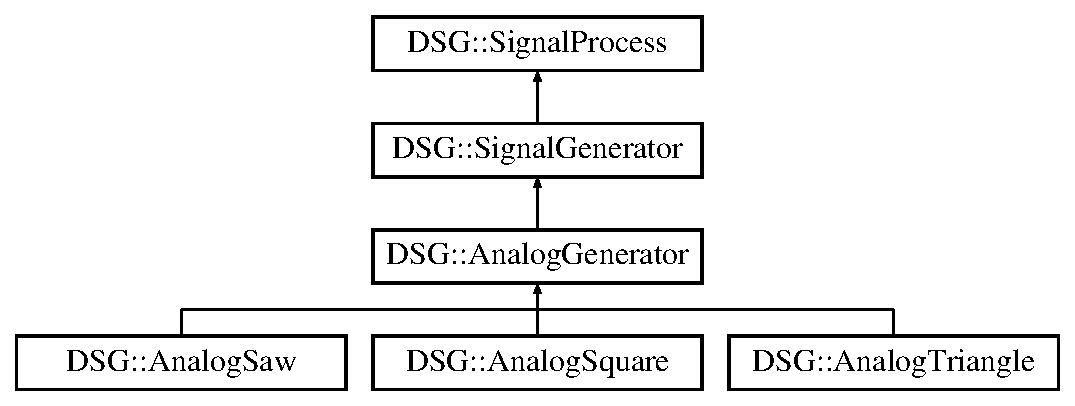
\includegraphics[height=4.000000cm]{classDSG_1_1AnalogGenerator}
\end{center}
\end{figure}
\subsection*{Public Member Functions}
\begin{DoxyCompactItemize}
\item 
\hyperlink{classDSG_1_1AnalogGenerator_a361c75a897c8984cd283bae8bdfd152e}{Analog\+Generator} ()
\item 
\hyperlink{classDSG_1_1AnalogGenerator_a13c3745554321cd94bc3121160641f4e}{Analog\+Generator} (double const \&frequency, double const \&phase\+\_\+offset)
\item 
virtual \hyperlink{classDSG_1_1AnalogGenerator_ae180f86033e38d3a5fcd8caecfb518e8}{$\sim$\+Analog\+Generator} ()
\item 
virtual bool \hyperlink{classDSG_1_1AnalogGenerator_ac50033964304239b514b7ee9d064bc75}{Perform} (\hyperlink{classDSG_1_1Sample}{Sample} \&signal)
\item 
virtual bool \hyperlink{classDSG_1_1AnalogGenerator_a1b4f1d4af926fcc3e9571db7960c8706}{Perform} (\hyperlink{classDSG_1_1RingBuffer}{Ring\+Buffer} \&signal)
\item 
virtual bool \hyperlink{classDSG_1_1SignalProcess_afdb8220100418893950c1161dd24db67}{Perform} (\hyperlink{classDSG_1_1Sample_aaf2e30d73911eccea99b53eeee15b612}{Sample\+::\+Sample} \&signal)=0
\item 
virtual double const \& \hyperlink{classDSG_1_1SignalGenerator_aedac746c5a70818d120858542ecb7c45}{Frequency} () const 
\item 
virtual double const \& \hyperlink{classDSG_1_1SignalGenerator_ae3ce8d45bafabbd86a0f535b15c3cd46}{Frequency} (double const \&value)
\item 
virtual double const \& \hyperlink{classDSG_1_1SignalGenerator_a1ce521847edd0b837fd840998f906b4b}{Phase\+Offset} () const 
\item 
virtual double const \& \hyperlink{classDSG_1_1SignalGenerator_a08b71b1f30ba65e629642c570291dc0e}{Phase\+Offset} (double const \&value)
\end{DoxyCompactItemize}
\subsection*{Protected Member Functions}
\begin{DoxyCompactItemize}
\item 
double \hyperlink{classDSG_1_1SignalGenerator_ac0d781b8673b3a283bf7c133290ede50}{\+\_\+pstep} ()
\item 
double \hyperlink{classDSG_1_1SignalGenerator_ae660eb4caa88b8d278f8d24d0908a487}{\+\_\+pstep\+\_\+rad} ()
\item 
void \hyperlink{classDSG_1_1SignalGenerator_a05baccb38d1e52860d4fcf7cb8430efc}{\+\_\+psync} ()
\end{DoxyCompactItemize}
\subsection*{Protected Attributes}
\begin{DoxyCompactItemize}
\item 
\hyperlink{classDSG_1_1Sample}{Sample} \hyperlink{classDSG_1_1AnalogGenerator_ac88ad591cac37f636c2f7b460480bef9}{\+\_\+sample}
\item 
double \hyperlink{classDSG_1_1SignalGenerator_aa10f6c85d9adee901139ea7fb346f39d}{\+\_\+rate}
\item 
double \hyperlink{classDSG_1_1SignalGenerator_a67e296e3506dcdf09402c667cddff9ac}{\+\_\+frequency}
\item 
double \hyperlink{classDSG_1_1SignalGenerator_ac2271b582bf699275f077ecb642a8cd9}{\+\_\+phasor}
\end{DoxyCompactItemize}


\subsection{Detailed Description}


Definition at line 17 of file Analog\+Generator.\+h.



\subsection{Constructor \& Destructor Documentation}
\hypertarget{classDSG_1_1AnalogGenerator_a361c75a897c8984cd283bae8bdfd152e}{\index{D\+S\+G\+::\+Analog\+Generator@{D\+S\+G\+::\+Analog\+Generator}!Analog\+Generator@{Analog\+Generator}}
\index{Analog\+Generator@{Analog\+Generator}!D\+S\+G\+::\+Analog\+Generator@{D\+S\+G\+::\+Analog\+Generator}}
\subsubsection[{Analog\+Generator}]{\setlength{\rightskip}{0pt plus 5cm}D\+S\+G\+::\+Analog\+Generator\+::\+Analog\+Generator (
\begin{DoxyParamCaption}
{}
\end{DoxyParamCaption}
)}}\label{classDSG_1_1AnalogGenerator_a361c75a897c8984cd283bae8bdfd152e}


Definition at line 9 of file Analog\+Generator.\+cpp.


\begin{DoxyCode}
9 :\hyperlink{classDSG_1_1SignalGenerator}{DSG::SignalGenerator}()\{\}
\end{DoxyCode}
\hypertarget{classDSG_1_1AnalogGenerator_a13c3745554321cd94bc3121160641f4e}{\index{D\+S\+G\+::\+Analog\+Generator@{D\+S\+G\+::\+Analog\+Generator}!Analog\+Generator@{Analog\+Generator}}
\index{Analog\+Generator@{Analog\+Generator}!D\+S\+G\+::\+Analog\+Generator@{D\+S\+G\+::\+Analog\+Generator}}
\subsubsection[{Analog\+Generator}]{\setlength{\rightskip}{0pt plus 5cm}D\+S\+G\+::\+Analog\+Generator\+::\+Analog\+Generator (
\begin{DoxyParamCaption}
\item[{double const \&}]{frequency, }
\item[{double const \&}]{phase\+\_\+offset}
\end{DoxyParamCaption}
)}}\label{classDSG_1_1AnalogGenerator_a13c3745554321cd94bc3121160641f4e}


Definition at line 10 of file Analog\+Generator.\+cpp.


\begin{DoxyCode}
10 :\hyperlink{classDSG_1_1SignalGenerator}{DSG::SignalGenerator}(frequency,phase\_offset)\{\}
\end{DoxyCode}
\hypertarget{classDSG_1_1AnalogGenerator_ae180f86033e38d3a5fcd8caecfb518e8}{\index{D\+S\+G\+::\+Analog\+Generator@{D\+S\+G\+::\+Analog\+Generator}!````~Analog\+Generator@{$\sim$\+Analog\+Generator}}
\index{````~Analog\+Generator@{$\sim$\+Analog\+Generator}!D\+S\+G\+::\+Analog\+Generator@{D\+S\+G\+::\+Analog\+Generator}}
\subsubsection[{$\sim$\+Analog\+Generator}]{\setlength{\rightskip}{0pt plus 5cm}D\+S\+G\+::\+Analog\+Generator\+::$\sim$\+Analog\+Generator (
\begin{DoxyParamCaption}
{}
\end{DoxyParamCaption}
)\hspace{0.3cm}{\ttfamily [virtual]}}}\label{classDSG_1_1AnalogGenerator_ae180f86033e38d3a5fcd8caecfb518e8}


Definition at line 11 of file Analog\+Generator.\+cpp.


\begin{DoxyCode}
11 \{\}
\end{DoxyCode}


\subsection{Member Function Documentation}
\hypertarget{classDSG_1_1SignalGenerator_ac0d781b8673b3a283bf7c133290ede50}{\index{D\+S\+G\+::\+Analog\+Generator@{D\+S\+G\+::\+Analog\+Generator}!\+\_\+pstep@{\+\_\+pstep}}
\index{\+\_\+pstep@{\+\_\+pstep}!D\+S\+G\+::\+Analog\+Generator@{D\+S\+G\+::\+Analog\+Generator}}
\subsubsection[{\+\_\+pstep}]{\setlength{\rightskip}{0pt plus 5cm}double D\+S\+G\+::\+Signal\+Generator\+::\+\_\+pstep (
\begin{DoxyParamCaption}
{}
\end{DoxyParamCaption}
)\hspace{0.3cm}{\ttfamily [inline]}, {\ttfamily [protected]}, {\ttfamily [inherited]}}}\label{classDSG_1_1SignalGenerator_ac0d781b8673b3a283bf7c133290ede50}


Definition at line 52 of file Signal\+Generator.\+h.


\begin{DoxyCode}
52                                          \{
53         value = \hyperlink{classDSG_1_1SignalGenerator_ac2271b582bf699275f077ecb642a8cd9}{\_phasor};
54         \hyperlink{classDSG_1_1SignalGenerator_ac2271b582bf699275f077ecb642a8cd9}{\_phasor}+=\hyperlink{classDSG_1_1SignalGenerator_aa10f6c85d9adee901139ea7fb346f39d}{\_rate};
55         \hyperlink{classDSG_1_1SignalGenerator_ac2271b582bf699275f077ecb642a8cd9}{\_phasor}>1?\hyperlink{classDSG_1_1SignalGenerator_ac2271b582bf699275f077ecb642a8cd9}{\_phasor}-=1:0;\textcolor{comment}{//cheaper cheaper %1}
56         \textcolor{comment}{//\_phasor -= (unsigned long)\_phasor;//cheaper %1}
57         \textcolor{keywordflow}{return} value;
58     \}
\end{DoxyCode}
\hypertarget{classDSG_1_1SignalGenerator_ae660eb4caa88b8d278f8d24d0908a487}{\index{D\+S\+G\+::\+Analog\+Generator@{D\+S\+G\+::\+Analog\+Generator}!\+\_\+pstep\+\_\+rad@{\+\_\+pstep\+\_\+rad}}
\index{\+\_\+pstep\+\_\+rad@{\+\_\+pstep\+\_\+rad}!D\+S\+G\+::\+Analog\+Generator@{D\+S\+G\+::\+Analog\+Generator}}
\subsubsection[{\+\_\+pstep\+\_\+rad}]{\setlength{\rightskip}{0pt plus 5cm}double D\+S\+G\+::\+Signal\+Generator\+::\+\_\+pstep\+\_\+rad (
\begin{DoxyParamCaption}
{}
\end{DoxyParamCaption}
)\hspace{0.3cm}{\ttfamily [inline]}, {\ttfamily [protected]}, {\ttfamily [inherited]}}}\label{classDSG_1_1SignalGenerator_ae660eb4caa88b8d278f8d24d0908a487}


Definition at line 59 of file Signal\+Generator.\+h.


\begin{DoxyCode}
59                                              \{
60         \textcolor{keywordflow}{return} \hyperlink{PI_8h_a4912c64aec0c943b7985db6cb61ff83a}{TWOPI} * \hyperlink{classDSG_1_1SignalGenerator_ac0d781b8673b3a283bf7c133290ede50}{\_pstep}();
61     \}
\end{DoxyCode}
\hypertarget{classDSG_1_1SignalGenerator_a05baccb38d1e52860d4fcf7cb8430efc}{\index{D\+S\+G\+::\+Analog\+Generator@{D\+S\+G\+::\+Analog\+Generator}!\+\_\+psync@{\+\_\+psync}}
\index{\+\_\+psync@{\+\_\+psync}!D\+S\+G\+::\+Analog\+Generator@{D\+S\+G\+::\+Analog\+Generator}}
\subsubsection[{\+\_\+psync}]{\setlength{\rightskip}{0pt plus 5cm}void D\+S\+G\+::\+Signal\+Generator\+::\+\_\+psync (
\begin{DoxyParamCaption}
{}
\end{DoxyParamCaption}
)\hspace{0.3cm}{\ttfamily [inline]}, {\ttfamily [protected]}, {\ttfamily [inherited]}}}\label{classDSG_1_1SignalGenerator_a05baccb38d1e52860d4fcf7cb8430efc}


Definition at line 62 of file Signal\+Generator.\+h.


\begin{DoxyCode}
62                                        \{
63         \hyperlink{classDSG_1_1SignalGenerator_ac2271b582bf699275f077ecb642a8cd9}{\_phasor} = \_phase\_offset;
64     \}
\end{DoxyCode}
\hypertarget{classDSG_1_1SignalGenerator_aedac746c5a70818d120858542ecb7c45}{\index{D\+S\+G\+::\+Analog\+Generator@{D\+S\+G\+::\+Analog\+Generator}!Frequency@{Frequency}}
\index{Frequency@{Frequency}!D\+S\+G\+::\+Analog\+Generator@{D\+S\+G\+::\+Analog\+Generator}}
\subsubsection[{Frequency}]{\setlength{\rightskip}{0pt plus 5cm}double const \& D\+S\+G\+::\+Signal\+Generator\+::\+Frequency (
\begin{DoxyParamCaption}
{}
\end{DoxyParamCaption}
) const\hspace{0.3cm}{\ttfamily [virtual]}, {\ttfamily [inherited]}}}\label{classDSG_1_1SignalGenerator_aedac746c5a70818d120858542ecb7c45}


Definition at line 14 of file Signal\+Generator.\+cpp.


\begin{DoxyCode}
14                                                 \{
15     \textcolor{keywordflow}{return} \hyperlink{classDSG_1_1SignalGenerator_a67e296e3506dcdf09402c667cddff9ac}{\_frequency};
16 \}
\end{DoxyCode}
\hypertarget{classDSG_1_1SignalGenerator_ae3ce8d45bafabbd86a0f535b15c3cd46}{\index{D\+S\+G\+::\+Analog\+Generator@{D\+S\+G\+::\+Analog\+Generator}!Frequency@{Frequency}}
\index{Frequency@{Frequency}!D\+S\+G\+::\+Analog\+Generator@{D\+S\+G\+::\+Analog\+Generator}}
\subsubsection[{Frequency}]{\setlength{\rightskip}{0pt plus 5cm}double const \& D\+S\+G\+::\+Signal\+Generator\+::\+Frequency (
\begin{DoxyParamCaption}
\item[{double const \&}]{value}
\end{DoxyParamCaption}
)\hspace{0.3cm}{\ttfamily [virtual]}, {\ttfamily [inherited]}}}\label{classDSG_1_1SignalGenerator_ae3ce8d45bafabbd86a0f535b15c3cd46}


Reimplemented in \hyperlink{classDSG_1_1BLIT_a67b698a54f37c361945cae3e137af76f}{D\+S\+G\+::\+B\+L\+I\+T}, \hyperlink{classDSG_1_1FourierTriangle_aebb275eee9fb923636a8db5e4aa90b39}{D\+S\+G\+::\+Fourier\+Triangle}, \hyperlink{classDSG_1_1FourierSaw_a929602365c9b29f30f523fa07a29966e}{D\+S\+G\+::\+Fourier\+Saw}, and \hyperlink{classDSG_1_1FourierSquare_a80f94eabad633e105cfa673fdee332d6}{D\+S\+G\+::\+Fourier\+Square}.



Definition at line 17 of file Signal\+Generator.\+cpp.


\begin{DoxyCode}
17                                                               \{
18     \hyperlink{classDSG_1_1SignalGenerator_a67e296e3506dcdf09402c667cddff9ac}{\_frequency} = value;
19     \hyperlink{classDSG_1_1SignalGenerator_aa10f6c85d9adee901139ea7fb346f39d}{\_rate} = \hyperlink{classDSG_1_1SignalGenerator_a67e296e3506dcdf09402c667cddff9ac}{\_frequency}/ \hyperlink{namespaceDSG_a0c5c3a251b3688398da18138c5efe4bf}{Sample\_Rate}();
20     \textcolor{keywordflow}{return} \hyperlink{classDSG_1_1SignalGenerator_a67e296e3506dcdf09402c667cddff9ac}{\_frequency};
21 \}
\end{DoxyCode}
\hypertarget{classDSG_1_1SignalProcess_afdb8220100418893950c1161dd24db67}{\index{D\+S\+G\+::\+Analog\+Generator@{D\+S\+G\+::\+Analog\+Generator}!Perform@{Perform}}
\index{Perform@{Perform}!D\+S\+G\+::\+Analog\+Generator@{D\+S\+G\+::\+Analog\+Generator}}
\subsubsection[{Perform}]{\setlength{\rightskip}{0pt plus 5cm}virtual bool D\+S\+G\+::\+Signal\+Process\+::\+Perform (
\begin{DoxyParamCaption}
\item[{{\bf Sample\+::\+Sample} \&}]{signal}
\end{DoxyParamCaption}
)\hspace{0.3cm}{\ttfamily [inline]}, {\ttfamily [pure virtual]}, {\ttfamily [inherited]}}}\label{classDSG_1_1SignalProcess_afdb8220100418893950c1161dd24db67}
\hypertarget{classDSG_1_1AnalogGenerator_ac50033964304239b514b7ee9d064bc75}{\index{D\+S\+G\+::\+Analog\+Generator@{D\+S\+G\+::\+Analog\+Generator}!Perform@{Perform}}
\index{Perform@{Perform}!D\+S\+G\+::\+Analog\+Generator@{D\+S\+G\+::\+Analog\+Generator}}
\subsubsection[{Perform}]{\setlength{\rightskip}{0pt plus 5cm}bool D\+S\+G\+::\+Analog\+Generator\+::\+Perform (
\begin{DoxyParamCaption}
\item[{{\bf Sample} \&}]{signal}
\end{DoxyParamCaption}
)\hspace{0.3cm}{\ttfamily [inline]}, {\ttfamily [virtual]}}}\label{classDSG_1_1AnalogGenerator_ac50033964304239b514b7ee9d064bc75}


Reimplemented from \hyperlink{classDSG_1_1SignalGenerator_a95d485b68d874938ac93644b121607b9}{D\+S\+G\+::\+Signal\+Generator}.



Reimplemented in \hyperlink{classDSG_1_1AnalogSaw_ae52d07d0d03f6f1fb92c012cc52ae3eb}{D\+S\+G\+::\+Analog\+Saw}, \hyperlink{classDSG_1_1AnalogSquare_a93a4b464545a32f72491d3df490fd3f7}{D\+S\+G\+::\+Analog\+Square}, and \hyperlink{classDSG_1_1AnalogTriangle_ac3edb87c395763d6894672b471850b05}{D\+S\+G\+::\+Analog\+Triangle}.



Definition at line 27 of file Analog\+Generator.\+h.


\begin{DoxyCode}
27                                                        \{
28         signal = 0;
29         \textcolor{keywordflow}{return} \textcolor{keyword}{false};
30     \}
\end{DoxyCode}
\hypertarget{classDSG_1_1AnalogGenerator_a1b4f1d4af926fcc3e9571db7960c8706}{\index{D\+S\+G\+::\+Analog\+Generator@{D\+S\+G\+::\+Analog\+Generator}!Perform@{Perform}}
\index{Perform@{Perform}!D\+S\+G\+::\+Analog\+Generator@{D\+S\+G\+::\+Analog\+Generator}}
\subsubsection[{Perform}]{\setlength{\rightskip}{0pt plus 5cm}bool D\+S\+G\+::\+Analog\+Generator\+::\+Perform (
\begin{DoxyParamCaption}
\item[{{\bf Ring\+Buffer} \&}]{signal}
\end{DoxyParamCaption}
)\hspace{0.3cm}{\ttfamily [inline]}, {\ttfamily [virtual]}}}\label{classDSG_1_1AnalogGenerator_a1b4f1d4af926fcc3e9571db7960c8706}


Reimplemented from \hyperlink{classDSG_1_1SignalGenerator_abaa9aecd00b792d46166b91524b42db6}{D\+S\+G\+::\+Signal\+Generator}.



Reimplemented in \hyperlink{classDSG_1_1AnalogSaw_a14dbd5c7faf6559b9ea79f8eb1ad6af5}{D\+S\+G\+::\+Analog\+Saw}, \hyperlink{classDSG_1_1AnalogSquare_a1d9c8a380775a7e4f6e0aa8fb1b05af6}{D\+S\+G\+::\+Analog\+Square}, and \hyperlink{classDSG_1_1AnalogTriangle_a9456183af28d98ccf3daa85b8ad12b52}{D\+S\+G\+::\+Analog\+Triangle}.



Definition at line 31 of file Analog\+Generator.\+h.


\begin{DoxyCode}
31                                                            \{
32         signal.Flush();
33         \textcolor{keywordflow}{while} (!signal.Full()) \{
34             \textcolor{keywordflow}{if} (\hyperlink{classDSG_1_1AnalogGenerator_ac50033964304239b514b7ee9d064bc75}{Perform}(\hyperlink{classDSG_1_1AnalogGenerator_ac88ad591cac37f636c2f7b460480bef9}{\_sample})) \{
35                 \textcolor{keywordflow}{if}(signal.Write(\hyperlink{classDSG_1_1AnalogGenerator_ac88ad591cac37f636c2f7b460480bef9}{\_sample}))\{
36                 \}\textcolor{keywordflow}{else} \textcolor{keywordflow}{return} \textcolor{keyword}{false};
37             \}\textcolor{keywordflow}{else} \textcolor{keywordflow}{return} \textcolor{keyword}{false};
38         \}\textcolor{keywordflow}{return} \textcolor{keyword}{true};
39     \}
\end{DoxyCode}
\hypertarget{classDSG_1_1SignalGenerator_a1ce521847edd0b837fd840998f906b4b}{\index{D\+S\+G\+::\+Analog\+Generator@{D\+S\+G\+::\+Analog\+Generator}!Phase\+Offset@{Phase\+Offset}}
\index{Phase\+Offset@{Phase\+Offset}!D\+S\+G\+::\+Analog\+Generator@{D\+S\+G\+::\+Analog\+Generator}}
\subsubsection[{Phase\+Offset}]{\setlength{\rightskip}{0pt plus 5cm}double const \& D\+S\+G\+::\+Signal\+Generator\+::\+Phase\+Offset (
\begin{DoxyParamCaption}
{}
\end{DoxyParamCaption}
) const\hspace{0.3cm}{\ttfamily [virtual]}, {\ttfamily [inherited]}}}\label{classDSG_1_1SignalGenerator_a1ce521847edd0b837fd840998f906b4b}


Definition at line 22 of file Signal\+Generator.\+cpp.


\begin{DoxyCode}
22                                                   \{
23     \textcolor{keywordflow}{return} \_phase\_offset;
24 \}
\end{DoxyCode}
\hypertarget{classDSG_1_1SignalGenerator_a08b71b1f30ba65e629642c570291dc0e}{\index{D\+S\+G\+::\+Analog\+Generator@{D\+S\+G\+::\+Analog\+Generator}!Phase\+Offset@{Phase\+Offset}}
\index{Phase\+Offset@{Phase\+Offset}!D\+S\+G\+::\+Analog\+Generator@{D\+S\+G\+::\+Analog\+Generator}}
\subsubsection[{Phase\+Offset}]{\setlength{\rightskip}{0pt plus 5cm}double const \& D\+S\+G\+::\+Signal\+Generator\+::\+Phase\+Offset (
\begin{DoxyParamCaption}
\item[{double const \&}]{value}
\end{DoxyParamCaption}
)\hspace{0.3cm}{\ttfamily [virtual]}, {\ttfamily [inherited]}}}\label{classDSG_1_1SignalGenerator_a08b71b1f30ba65e629642c570291dc0e}


Definition at line 25 of file Signal\+Generator.\+cpp.


\begin{DoxyCode}
25                                                                 \{
26     \_phase\_offset-=value;
27     \hyperlink{classDSG_1_1SignalGenerator_ac2271b582bf699275f077ecb642a8cd9}{\_phasor}-=\_phase\_offset;
28     \_phase\_offset=value;
29     \textcolor{keywordflow}{return} \_phase\_offset;
30 \}\end{DoxyCode}


\subsection{Member Data Documentation}
\hypertarget{classDSG_1_1SignalGenerator_a67e296e3506dcdf09402c667cddff9ac}{\index{D\+S\+G\+::\+Analog\+Generator@{D\+S\+G\+::\+Analog\+Generator}!\+\_\+frequency@{\+\_\+frequency}}
\index{\+\_\+frequency@{\+\_\+frequency}!D\+S\+G\+::\+Analog\+Generator@{D\+S\+G\+::\+Analog\+Generator}}
\subsubsection[{\+\_\+frequency}]{\setlength{\rightskip}{0pt plus 5cm}double D\+S\+G\+::\+Signal\+Generator\+::\+\_\+frequency\hspace{0.3cm}{\ttfamily [protected]}, {\ttfamily [inherited]}}}\label{classDSG_1_1SignalGenerator_a67e296e3506dcdf09402c667cddff9ac}


Definition at line 28 of file Signal\+Generator.\+h.

\hypertarget{classDSG_1_1SignalGenerator_ac2271b582bf699275f077ecb642a8cd9}{\index{D\+S\+G\+::\+Analog\+Generator@{D\+S\+G\+::\+Analog\+Generator}!\+\_\+phasor@{\+\_\+phasor}}
\index{\+\_\+phasor@{\+\_\+phasor}!D\+S\+G\+::\+Analog\+Generator@{D\+S\+G\+::\+Analog\+Generator}}
\subsubsection[{\+\_\+phasor}]{\setlength{\rightskip}{0pt plus 5cm}double D\+S\+G\+::\+Signal\+Generator\+::\+\_\+phasor\hspace{0.3cm}{\ttfamily [protected]}, {\ttfamily [inherited]}}}\label{classDSG_1_1SignalGenerator_ac2271b582bf699275f077ecb642a8cd9}


Definition at line 38 of file Signal\+Generator.\+h.

\hypertarget{classDSG_1_1SignalGenerator_aa10f6c85d9adee901139ea7fb346f39d}{\index{D\+S\+G\+::\+Analog\+Generator@{D\+S\+G\+::\+Analog\+Generator}!\+\_\+rate@{\+\_\+rate}}
\index{\+\_\+rate@{\+\_\+rate}!D\+S\+G\+::\+Analog\+Generator@{D\+S\+G\+::\+Analog\+Generator}}
\subsubsection[{\+\_\+rate}]{\setlength{\rightskip}{0pt plus 5cm}double D\+S\+G\+::\+Signal\+Generator\+::\+\_\+rate\hspace{0.3cm}{\ttfamily [protected]}, {\ttfamily [inherited]}}}\label{classDSG_1_1SignalGenerator_aa10f6c85d9adee901139ea7fb346f39d}


Definition at line 27 of file Signal\+Generator.\+h.

\hypertarget{classDSG_1_1AnalogGenerator_ac88ad591cac37f636c2f7b460480bef9}{\index{D\+S\+G\+::\+Analog\+Generator@{D\+S\+G\+::\+Analog\+Generator}!\+\_\+sample@{\+\_\+sample}}
\index{\+\_\+sample@{\+\_\+sample}!D\+S\+G\+::\+Analog\+Generator@{D\+S\+G\+::\+Analog\+Generator}}
\subsubsection[{\+\_\+sample}]{\setlength{\rightskip}{0pt plus 5cm}{\bf Sample} D\+S\+G\+::\+Analog\+Generator\+::\+\_\+sample\hspace{0.3cm}{\ttfamily [protected]}}}\label{classDSG_1_1AnalogGenerator_ac88ad591cac37f636c2f7b460480bef9}


Definition at line 25 of file Analog\+Generator.\+h.



The documentation for this class was generated from the following files\+:\begin{DoxyCompactItemize}
\item 
/\+Users/alexanderzywicki/\+Documents/\+School\+\_\+\+Stuff/\+Fall\+\_\+2014/\+Digital\+\_\+\+Signal\+\_\+\+Generation\+\_\+and\+\_\+\+Analysis/src/include/\hyperlink{AnalogGenerator_8h}{Analog\+Generator.\+h}\item 
/\+Users/alexanderzywicki/\+Documents/\+School\+\_\+\+Stuff/\+Fall\+\_\+2014/\+Digital\+\_\+\+Signal\+\_\+\+Generation\+\_\+and\+\_\+\+Analysis/src/\hyperlink{AnalogGenerator_8cpp}{Analog\+Generator.\+cpp}\end{DoxyCompactItemize}

\hypertarget{classDSG_1_1AnalogSaw}{\section{D\+S\+G\+:\+:Analog\+Saw Class Reference}
\label{classDSG_1_1AnalogSaw}\index{D\+S\+G\+::\+Analog\+Saw@{D\+S\+G\+::\+Analog\+Saw}}
}


{\ttfamily \#include $<$Analog\+Saw.\+h$>$}

Inheritance diagram for D\+S\+G\+:\+:Analog\+Saw\+:\begin{figure}[H]
\begin{center}
\leavevmode
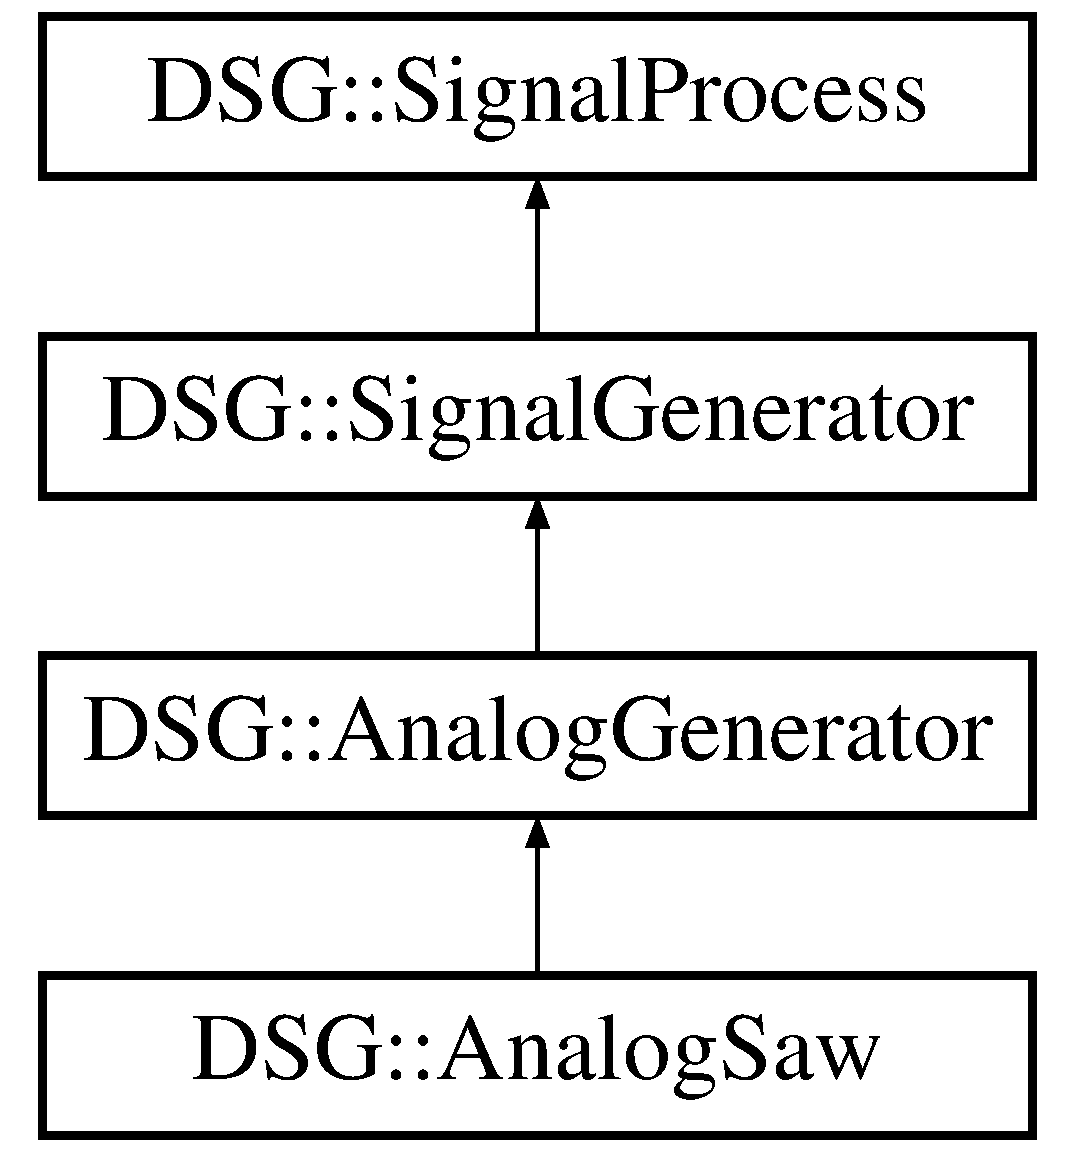
\includegraphics[height=4.000000cm]{classDSG_1_1AnalogSaw}
\end{center}
\end{figure}
\subsection*{Public Member Functions}
\begin{DoxyCompactItemize}
\item 
\hyperlink{classDSG_1_1AnalogSaw_ae070d24c8d7253be67ffec52445bfc40}{Analog\+Saw} ()
\item 
\hyperlink{classDSG_1_1AnalogSaw_a2b6a21de7b41e541b1dfb016a7c92c3e}{Analog\+Saw} (double const \&frequency, double const \&phase\+\_\+offset)
\item 
virtual \hyperlink{classDSG_1_1AnalogSaw_a30b1d3ac3a8c6c2c093f861e3ead29a8}{$\sim$\+Analog\+Saw} ()
\item 
virtual bool \hyperlink{classDSG_1_1AnalogSaw_ae52d07d0d03f6f1fb92c012cc52ae3eb}{Perform} (\hyperlink{classDSG_1_1Sample}{Sample} \&signal)
\item 
virtual bool \hyperlink{classDSG_1_1AnalogSaw_a14dbd5c7faf6559b9ea79f8eb1ad6af5}{Perform} (\hyperlink{classDSG_1_1RingBuffer}{Ring\+Buffer} \&signal)
\item 
virtual bool \hyperlink{classDSG_1_1SignalProcess_afdb8220100418893950c1161dd24db67}{Perform} (\hyperlink{classDSG_1_1Sample_aaf2e30d73911eccea99b53eeee15b612}{Sample\+::\+Sample} \&signal)=0
\item 
virtual double const \& \hyperlink{classDSG_1_1SignalGenerator_aedac746c5a70818d120858542ecb7c45}{Frequency} () const 
\item 
virtual double const \& \hyperlink{classDSG_1_1SignalGenerator_ae3ce8d45bafabbd86a0f535b15c3cd46}{Frequency} (double const \&value)
\item 
virtual double const \& \hyperlink{classDSG_1_1SignalGenerator_a1ce521847edd0b837fd840998f906b4b}{Phase\+Offset} () const 
\item 
virtual double const \& \hyperlink{classDSG_1_1SignalGenerator_a08b71b1f30ba65e629642c570291dc0e}{Phase\+Offset} (double const \&value)
\end{DoxyCompactItemize}
\subsection*{Protected Member Functions}
\begin{DoxyCompactItemize}
\item 
double \hyperlink{classDSG_1_1SignalGenerator_ac0d781b8673b3a283bf7c133290ede50}{\+\_\+pstep} ()
\item 
double \hyperlink{classDSG_1_1SignalGenerator_ae660eb4caa88b8d278f8d24d0908a487}{\+\_\+pstep\+\_\+rad} ()
\item 
void \hyperlink{classDSG_1_1SignalGenerator_a05baccb38d1e52860d4fcf7cb8430efc}{\+\_\+psync} ()
\end{DoxyCompactItemize}
\subsection*{Protected Attributes}
\begin{DoxyCompactItemize}
\item 
\hyperlink{classDSG_1_1Sample}{Sample} \hyperlink{classDSG_1_1AnalogGenerator_ac88ad591cac37f636c2f7b460480bef9}{\+\_\+sample}
\item 
double \hyperlink{classDSG_1_1SignalGenerator_aa10f6c85d9adee901139ea7fb346f39d}{\+\_\+rate}
\item 
double \hyperlink{classDSG_1_1SignalGenerator_a67e296e3506dcdf09402c667cddff9ac}{\+\_\+frequency}
\item 
double \hyperlink{classDSG_1_1SignalGenerator_ac2271b582bf699275f077ecb642a8cd9}{\+\_\+phasor}
\end{DoxyCompactItemize}


\subsection{Detailed Description}


Definition at line 14 of file Analog\+Saw.\+h.



\subsection{Constructor \& Destructor Documentation}
\hypertarget{classDSG_1_1AnalogSaw_ae070d24c8d7253be67ffec52445bfc40}{\index{D\+S\+G\+::\+Analog\+Saw@{D\+S\+G\+::\+Analog\+Saw}!Analog\+Saw@{Analog\+Saw}}
\index{Analog\+Saw@{Analog\+Saw}!D\+S\+G\+::\+Analog\+Saw@{D\+S\+G\+::\+Analog\+Saw}}
\subsubsection[{Analog\+Saw}]{\setlength{\rightskip}{0pt plus 5cm}D\+S\+G\+::\+Analog\+Saw\+::\+Analog\+Saw (
\begin{DoxyParamCaption}
{}
\end{DoxyParamCaption}
)}}\label{classDSG_1_1AnalogSaw_ae070d24c8d7253be67ffec52445bfc40}


Definition at line 9 of file Analog\+Saw.\+cpp.


\begin{DoxyCode}
9 :\hyperlink{classDSG_1_1AnalogGenerator}{DSG::AnalogGenerator}()\{\}
\end{DoxyCode}
\hypertarget{classDSG_1_1AnalogSaw_a2b6a21de7b41e541b1dfb016a7c92c3e}{\index{D\+S\+G\+::\+Analog\+Saw@{D\+S\+G\+::\+Analog\+Saw}!Analog\+Saw@{Analog\+Saw}}
\index{Analog\+Saw@{Analog\+Saw}!D\+S\+G\+::\+Analog\+Saw@{D\+S\+G\+::\+Analog\+Saw}}
\subsubsection[{Analog\+Saw}]{\setlength{\rightskip}{0pt plus 5cm}D\+S\+G\+::\+Analog\+Saw\+::\+Analog\+Saw (
\begin{DoxyParamCaption}
\item[{double const \&}]{frequency, }
\item[{double const \&}]{phase\+\_\+offset}
\end{DoxyParamCaption}
)}}\label{classDSG_1_1AnalogSaw_a2b6a21de7b41e541b1dfb016a7c92c3e}


Definition at line 10 of file Analog\+Saw.\+cpp.


\begin{DoxyCode}
10 :\hyperlink{classDSG_1_1AnalogGenerator}{DSG::AnalogGenerator}(frequency,phase\_offset)\{\}
\end{DoxyCode}
\hypertarget{classDSG_1_1AnalogSaw_a30b1d3ac3a8c6c2c093f861e3ead29a8}{\index{D\+S\+G\+::\+Analog\+Saw@{D\+S\+G\+::\+Analog\+Saw}!````~Analog\+Saw@{$\sim$\+Analog\+Saw}}
\index{````~Analog\+Saw@{$\sim$\+Analog\+Saw}!D\+S\+G\+::\+Analog\+Saw@{D\+S\+G\+::\+Analog\+Saw}}
\subsubsection[{$\sim$\+Analog\+Saw}]{\setlength{\rightskip}{0pt plus 5cm}D\+S\+G\+::\+Analog\+Saw\+::$\sim$\+Analog\+Saw (
\begin{DoxyParamCaption}
{}
\end{DoxyParamCaption}
)\hspace{0.3cm}{\ttfamily [virtual]}}}\label{classDSG_1_1AnalogSaw_a30b1d3ac3a8c6c2c093f861e3ead29a8}


Definition at line 11 of file Analog\+Saw.\+cpp.


\begin{DoxyCode}
11 \{\}\end{DoxyCode}


\subsection{Member Function Documentation}
\hypertarget{classDSG_1_1SignalGenerator_ac0d781b8673b3a283bf7c133290ede50}{\index{D\+S\+G\+::\+Analog\+Saw@{D\+S\+G\+::\+Analog\+Saw}!\+\_\+pstep@{\+\_\+pstep}}
\index{\+\_\+pstep@{\+\_\+pstep}!D\+S\+G\+::\+Analog\+Saw@{D\+S\+G\+::\+Analog\+Saw}}
\subsubsection[{\+\_\+pstep}]{\setlength{\rightskip}{0pt plus 5cm}double D\+S\+G\+::\+Signal\+Generator\+::\+\_\+pstep (
\begin{DoxyParamCaption}
{}
\end{DoxyParamCaption}
)\hspace{0.3cm}{\ttfamily [inline]}, {\ttfamily [protected]}, {\ttfamily [inherited]}}}\label{classDSG_1_1SignalGenerator_ac0d781b8673b3a283bf7c133290ede50}


Definition at line 52 of file Signal\+Generator.\+h.


\begin{DoxyCode}
52                                          \{
53         value = \hyperlink{classDSG_1_1SignalGenerator_ac2271b582bf699275f077ecb642a8cd9}{\_phasor};
54         \hyperlink{classDSG_1_1SignalGenerator_ac2271b582bf699275f077ecb642a8cd9}{\_phasor}+=\hyperlink{classDSG_1_1SignalGenerator_aa10f6c85d9adee901139ea7fb346f39d}{\_rate};
55         \hyperlink{classDSG_1_1SignalGenerator_ac2271b582bf699275f077ecb642a8cd9}{\_phasor}>1?\hyperlink{classDSG_1_1SignalGenerator_ac2271b582bf699275f077ecb642a8cd9}{\_phasor}-=1:0;\textcolor{comment}{//cheaper cheaper %1}
56         \textcolor{comment}{//\_phasor -= (unsigned long)\_phasor;//cheaper %1}
57         \textcolor{keywordflow}{return} value;
58     \}
\end{DoxyCode}
\hypertarget{classDSG_1_1SignalGenerator_ae660eb4caa88b8d278f8d24d0908a487}{\index{D\+S\+G\+::\+Analog\+Saw@{D\+S\+G\+::\+Analog\+Saw}!\+\_\+pstep\+\_\+rad@{\+\_\+pstep\+\_\+rad}}
\index{\+\_\+pstep\+\_\+rad@{\+\_\+pstep\+\_\+rad}!D\+S\+G\+::\+Analog\+Saw@{D\+S\+G\+::\+Analog\+Saw}}
\subsubsection[{\+\_\+pstep\+\_\+rad}]{\setlength{\rightskip}{0pt plus 5cm}double D\+S\+G\+::\+Signal\+Generator\+::\+\_\+pstep\+\_\+rad (
\begin{DoxyParamCaption}
{}
\end{DoxyParamCaption}
)\hspace{0.3cm}{\ttfamily [inline]}, {\ttfamily [protected]}, {\ttfamily [inherited]}}}\label{classDSG_1_1SignalGenerator_ae660eb4caa88b8d278f8d24d0908a487}


Definition at line 59 of file Signal\+Generator.\+h.


\begin{DoxyCode}
59                                              \{
60         \textcolor{keywordflow}{return} \hyperlink{PI_8h_a4912c64aec0c943b7985db6cb61ff83a}{TWOPI} * \hyperlink{classDSG_1_1SignalGenerator_ac0d781b8673b3a283bf7c133290ede50}{\_pstep}();
61     \}
\end{DoxyCode}
\hypertarget{classDSG_1_1SignalGenerator_a05baccb38d1e52860d4fcf7cb8430efc}{\index{D\+S\+G\+::\+Analog\+Saw@{D\+S\+G\+::\+Analog\+Saw}!\+\_\+psync@{\+\_\+psync}}
\index{\+\_\+psync@{\+\_\+psync}!D\+S\+G\+::\+Analog\+Saw@{D\+S\+G\+::\+Analog\+Saw}}
\subsubsection[{\+\_\+psync}]{\setlength{\rightskip}{0pt plus 5cm}void D\+S\+G\+::\+Signal\+Generator\+::\+\_\+psync (
\begin{DoxyParamCaption}
{}
\end{DoxyParamCaption}
)\hspace{0.3cm}{\ttfamily [inline]}, {\ttfamily [protected]}, {\ttfamily [inherited]}}}\label{classDSG_1_1SignalGenerator_a05baccb38d1e52860d4fcf7cb8430efc}


Definition at line 62 of file Signal\+Generator.\+h.


\begin{DoxyCode}
62                                        \{
63         \hyperlink{classDSG_1_1SignalGenerator_ac2271b582bf699275f077ecb642a8cd9}{\_phasor} = \_phase\_offset;
64     \}
\end{DoxyCode}
\hypertarget{classDSG_1_1SignalGenerator_aedac746c5a70818d120858542ecb7c45}{\index{D\+S\+G\+::\+Analog\+Saw@{D\+S\+G\+::\+Analog\+Saw}!Frequency@{Frequency}}
\index{Frequency@{Frequency}!D\+S\+G\+::\+Analog\+Saw@{D\+S\+G\+::\+Analog\+Saw}}
\subsubsection[{Frequency}]{\setlength{\rightskip}{0pt plus 5cm}double const \& D\+S\+G\+::\+Signal\+Generator\+::\+Frequency (
\begin{DoxyParamCaption}
{}
\end{DoxyParamCaption}
) const\hspace{0.3cm}{\ttfamily [virtual]}, {\ttfamily [inherited]}}}\label{classDSG_1_1SignalGenerator_aedac746c5a70818d120858542ecb7c45}


Definition at line 14 of file Signal\+Generator.\+cpp.


\begin{DoxyCode}
14                                                 \{
15     \textcolor{keywordflow}{return} \hyperlink{classDSG_1_1SignalGenerator_a67e296e3506dcdf09402c667cddff9ac}{\_frequency};
16 \}
\end{DoxyCode}
\hypertarget{classDSG_1_1SignalGenerator_ae3ce8d45bafabbd86a0f535b15c3cd46}{\index{D\+S\+G\+::\+Analog\+Saw@{D\+S\+G\+::\+Analog\+Saw}!Frequency@{Frequency}}
\index{Frequency@{Frequency}!D\+S\+G\+::\+Analog\+Saw@{D\+S\+G\+::\+Analog\+Saw}}
\subsubsection[{Frequency}]{\setlength{\rightskip}{0pt plus 5cm}double const \& D\+S\+G\+::\+Signal\+Generator\+::\+Frequency (
\begin{DoxyParamCaption}
\item[{double const \&}]{value}
\end{DoxyParamCaption}
)\hspace{0.3cm}{\ttfamily [virtual]}, {\ttfamily [inherited]}}}\label{classDSG_1_1SignalGenerator_ae3ce8d45bafabbd86a0f535b15c3cd46}


Reimplemented in \hyperlink{classDSG_1_1BLIT_a67b698a54f37c361945cae3e137af76f}{D\+S\+G\+::\+B\+L\+I\+T}, \hyperlink{classDSG_1_1FourierTriangle_aebb275eee9fb923636a8db5e4aa90b39}{D\+S\+G\+::\+Fourier\+Triangle}, \hyperlink{classDSG_1_1FourierSaw_a929602365c9b29f30f523fa07a29966e}{D\+S\+G\+::\+Fourier\+Saw}, and \hyperlink{classDSG_1_1FourierSquare_a80f94eabad633e105cfa673fdee332d6}{D\+S\+G\+::\+Fourier\+Square}.



Definition at line 17 of file Signal\+Generator.\+cpp.


\begin{DoxyCode}
17                                                               \{
18     \hyperlink{classDSG_1_1SignalGenerator_a67e296e3506dcdf09402c667cddff9ac}{\_frequency} = value;
19     \hyperlink{classDSG_1_1SignalGenerator_aa10f6c85d9adee901139ea7fb346f39d}{\_rate} = \hyperlink{classDSG_1_1SignalGenerator_a67e296e3506dcdf09402c667cddff9ac}{\_frequency}/ \hyperlink{namespaceDSG_a0c5c3a251b3688398da18138c5efe4bf}{Sample\_Rate}();
20     \textcolor{keywordflow}{return} \hyperlink{classDSG_1_1SignalGenerator_a67e296e3506dcdf09402c667cddff9ac}{\_frequency};
21 \}
\end{DoxyCode}
\hypertarget{classDSG_1_1AnalogSaw_ae52d07d0d03f6f1fb92c012cc52ae3eb}{\index{D\+S\+G\+::\+Analog\+Saw@{D\+S\+G\+::\+Analog\+Saw}!Perform@{Perform}}
\index{Perform@{Perform}!D\+S\+G\+::\+Analog\+Saw@{D\+S\+G\+::\+Analog\+Saw}}
\subsubsection[{Perform}]{\setlength{\rightskip}{0pt plus 5cm}bool D\+S\+G\+::\+Analog\+Saw\+::\+Perform (
\begin{DoxyParamCaption}
\item[{{\bf Sample} \&}]{signal}
\end{DoxyParamCaption}
)\hspace{0.3cm}{\ttfamily [inline]}, {\ttfamily [virtual]}}}\label{classDSG_1_1AnalogSaw_ae52d07d0d03f6f1fb92c012cc52ae3eb}


Reimplemented from \hyperlink{classDSG_1_1AnalogGenerator_ac50033964304239b514b7ee9d064bc75}{D\+S\+G\+::\+Analog\+Generator}.



Definition at line 24 of file Analog\+Saw.\+h.


\begin{DoxyCode}
24                                                  \{
25         \textcolor{keywordtype}{double} value = \hyperlink{classDSG_1_1SignalGenerator_ac0d781b8673b3a283bf7c133290ede50}{\_pstep}();
26         
27         value-=0.5;
28         value*=2.0;
29         signal = value;
30         \textcolor{keywordflow}{return} \textcolor{keyword}{true};
31     \}
\end{DoxyCode}
\hypertarget{classDSG_1_1SignalProcess_afdb8220100418893950c1161dd24db67}{\index{D\+S\+G\+::\+Analog\+Saw@{D\+S\+G\+::\+Analog\+Saw}!Perform@{Perform}}
\index{Perform@{Perform}!D\+S\+G\+::\+Analog\+Saw@{D\+S\+G\+::\+Analog\+Saw}}
\subsubsection[{Perform}]{\setlength{\rightskip}{0pt plus 5cm}virtual bool D\+S\+G\+::\+Signal\+Process\+::\+Perform (
\begin{DoxyParamCaption}
\item[{{\bf Sample\+::\+Sample} \&}]{signal}
\end{DoxyParamCaption}
)\hspace{0.3cm}{\ttfamily [inline]}, {\ttfamily [pure virtual]}, {\ttfamily [inherited]}}}\label{classDSG_1_1SignalProcess_afdb8220100418893950c1161dd24db67}
\hypertarget{classDSG_1_1AnalogSaw_a14dbd5c7faf6559b9ea79f8eb1ad6af5}{\index{D\+S\+G\+::\+Analog\+Saw@{D\+S\+G\+::\+Analog\+Saw}!Perform@{Perform}}
\index{Perform@{Perform}!D\+S\+G\+::\+Analog\+Saw@{D\+S\+G\+::\+Analog\+Saw}}
\subsubsection[{Perform}]{\setlength{\rightskip}{0pt plus 5cm}bool D\+S\+G\+::\+Analog\+Saw\+::\+Perform (
\begin{DoxyParamCaption}
\item[{{\bf Ring\+Buffer} \&}]{signal}
\end{DoxyParamCaption}
)\hspace{0.3cm}{\ttfamily [inline]}, {\ttfamily [virtual]}}}\label{classDSG_1_1AnalogSaw_a14dbd5c7faf6559b9ea79f8eb1ad6af5}


Reimplemented from \hyperlink{classDSG_1_1AnalogGenerator_a1b4f1d4af926fcc3e9571db7960c8706}{D\+S\+G\+::\+Analog\+Generator}.



Definition at line 32 of file Analog\+Saw.\+h.


\begin{DoxyCode}
32                                                      \{
33         signal.Flush();
34         \textcolor{keywordflow}{while} (!signal.Full()) \{
35             \textcolor{keywordflow}{if} (\hyperlink{classDSG_1_1AnalogSaw_ae52d07d0d03f6f1fb92c012cc52ae3eb}{Perform}(\hyperlink{classDSG_1_1AnalogGenerator_ac88ad591cac37f636c2f7b460480bef9}{\_sample})) \{
36                 \textcolor{keywordflow}{if}(signal.Write(\hyperlink{classDSG_1_1AnalogGenerator_ac88ad591cac37f636c2f7b460480bef9}{\_sample}))\{
37                 \}\textcolor{keywordflow}{else} \textcolor{keywordflow}{return} \textcolor{keyword}{false};
38             \}\textcolor{keywordflow}{else} \textcolor{keywordflow}{return} \textcolor{keyword}{false};
39         \}\textcolor{keywordflow}{return} \textcolor{keyword}{true};
40     \}
\end{DoxyCode}
\hypertarget{classDSG_1_1SignalGenerator_a1ce521847edd0b837fd840998f906b4b}{\index{D\+S\+G\+::\+Analog\+Saw@{D\+S\+G\+::\+Analog\+Saw}!Phase\+Offset@{Phase\+Offset}}
\index{Phase\+Offset@{Phase\+Offset}!D\+S\+G\+::\+Analog\+Saw@{D\+S\+G\+::\+Analog\+Saw}}
\subsubsection[{Phase\+Offset}]{\setlength{\rightskip}{0pt plus 5cm}double const \& D\+S\+G\+::\+Signal\+Generator\+::\+Phase\+Offset (
\begin{DoxyParamCaption}
{}
\end{DoxyParamCaption}
) const\hspace{0.3cm}{\ttfamily [virtual]}, {\ttfamily [inherited]}}}\label{classDSG_1_1SignalGenerator_a1ce521847edd0b837fd840998f906b4b}


Definition at line 22 of file Signal\+Generator.\+cpp.


\begin{DoxyCode}
22                                                   \{
23     \textcolor{keywordflow}{return} \_phase\_offset;
24 \}
\end{DoxyCode}
\hypertarget{classDSG_1_1SignalGenerator_a08b71b1f30ba65e629642c570291dc0e}{\index{D\+S\+G\+::\+Analog\+Saw@{D\+S\+G\+::\+Analog\+Saw}!Phase\+Offset@{Phase\+Offset}}
\index{Phase\+Offset@{Phase\+Offset}!D\+S\+G\+::\+Analog\+Saw@{D\+S\+G\+::\+Analog\+Saw}}
\subsubsection[{Phase\+Offset}]{\setlength{\rightskip}{0pt plus 5cm}double const \& D\+S\+G\+::\+Signal\+Generator\+::\+Phase\+Offset (
\begin{DoxyParamCaption}
\item[{double const \&}]{value}
\end{DoxyParamCaption}
)\hspace{0.3cm}{\ttfamily [virtual]}, {\ttfamily [inherited]}}}\label{classDSG_1_1SignalGenerator_a08b71b1f30ba65e629642c570291dc0e}


Definition at line 25 of file Signal\+Generator.\+cpp.


\begin{DoxyCode}
25                                                                 \{
26     \_phase\_offset-=value;
27     \hyperlink{classDSG_1_1SignalGenerator_ac2271b582bf699275f077ecb642a8cd9}{\_phasor}-=\_phase\_offset;
28     \_phase\_offset=value;
29     \textcolor{keywordflow}{return} \_phase\_offset;
30 \}\end{DoxyCode}


\subsection{Member Data Documentation}
\hypertarget{classDSG_1_1SignalGenerator_a67e296e3506dcdf09402c667cddff9ac}{\index{D\+S\+G\+::\+Analog\+Saw@{D\+S\+G\+::\+Analog\+Saw}!\+\_\+frequency@{\+\_\+frequency}}
\index{\+\_\+frequency@{\+\_\+frequency}!D\+S\+G\+::\+Analog\+Saw@{D\+S\+G\+::\+Analog\+Saw}}
\subsubsection[{\+\_\+frequency}]{\setlength{\rightskip}{0pt plus 5cm}double D\+S\+G\+::\+Signal\+Generator\+::\+\_\+frequency\hspace{0.3cm}{\ttfamily [protected]}, {\ttfamily [inherited]}}}\label{classDSG_1_1SignalGenerator_a67e296e3506dcdf09402c667cddff9ac}


Definition at line 28 of file Signal\+Generator.\+h.

\hypertarget{classDSG_1_1SignalGenerator_ac2271b582bf699275f077ecb642a8cd9}{\index{D\+S\+G\+::\+Analog\+Saw@{D\+S\+G\+::\+Analog\+Saw}!\+\_\+phasor@{\+\_\+phasor}}
\index{\+\_\+phasor@{\+\_\+phasor}!D\+S\+G\+::\+Analog\+Saw@{D\+S\+G\+::\+Analog\+Saw}}
\subsubsection[{\+\_\+phasor}]{\setlength{\rightskip}{0pt plus 5cm}double D\+S\+G\+::\+Signal\+Generator\+::\+\_\+phasor\hspace{0.3cm}{\ttfamily [protected]}, {\ttfamily [inherited]}}}\label{classDSG_1_1SignalGenerator_ac2271b582bf699275f077ecb642a8cd9}


Definition at line 38 of file Signal\+Generator.\+h.

\hypertarget{classDSG_1_1SignalGenerator_aa10f6c85d9adee901139ea7fb346f39d}{\index{D\+S\+G\+::\+Analog\+Saw@{D\+S\+G\+::\+Analog\+Saw}!\+\_\+rate@{\+\_\+rate}}
\index{\+\_\+rate@{\+\_\+rate}!D\+S\+G\+::\+Analog\+Saw@{D\+S\+G\+::\+Analog\+Saw}}
\subsubsection[{\+\_\+rate}]{\setlength{\rightskip}{0pt plus 5cm}double D\+S\+G\+::\+Signal\+Generator\+::\+\_\+rate\hspace{0.3cm}{\ttfamily [protected]}, {\ttfamily [inherited]}}}\label{classDSG_1_1SignalGenerator_aa10f6c85d9adee901139ea7fb346f39d}


Definition at line 27 of file Signal\+Generator.\+h.

\hypertarget{classDSG_1_1AnalogGenerator_ac88ad591cac37f636c2f7b460480bef9}{\index{D\+S\+G\+::\+Analog\+Saw@{D\+S\+G\+::\+Analog\+Saw}!\+\_\+sample@{\+\_\+sample}}
\index{\+\_\+sample@{\+\_\+sample}!D\+S\+G\+::\+Analog\+Saw@{D\+S\+G\+::\+Analog\+Saw}}
\subsubsection[{\+\_\+sample}]{\setlength{\rightskip}{0pt plus 5cm}{\bf Sample} D\+S\+G\+::\+Analog\+Generator\+::\+\_\+sample\hspace{0.3cm}{\ttfamily [protected]}, {\ttfamily [inherited]}}}\label{classDSG_1_1AnalogGenerator_ac88ad591cac37f636c2f7b460480bef9}


Definition at line 25 of file Analog\+Generator.\+h.



The documentation for this class was generated from the following files\+:\begin{DoxyCompactItemize}
\item 
/\+Users/alexanderzywicki/\+Documents/\+School\+\_\+\+Stuff/\+Fall\+\_\+2014/\+Digital\+\_\+\+Signal\+\_\+\+Generation\+\_\+and\+\_\+\+Analysis/src/include/\hyperlink{AnalogSaw_8h}{Analog\+Saw.\+h}\item 
/\+Users/alexanderzywicki/\+Documents/\+School\+\_\+\+Stuff/\+Fall\+\_\+2014/\+Digital\+\_\+\+Signal\+\_\+\+Generation\+\_\+and\+\_\+\+Analysis/src/\hyperlink{AnalogSaw_8cpp}{Analog\+Saw.\+cpp}\end{DoxyCompactItemize}

\hypertarget{classDSG_1_1AnalogSquare}{\section{D\+S\+G\+:\+:Analog\+Square Class Reference}
\label{classDSG_1_1AnalogSquare}\index{D\+S\+G\+::\+Analog\+Square@{D\+S\+G\+::\+Analog\+Square}}
}


{\ttfamily \#include $<$Analog\+Square.\+h$>$}

Inheritance diagram for D\+S\+G\+:\+:Analog\+Square\+:\begin{figure}[H]
\begin{center}
\leavevmode
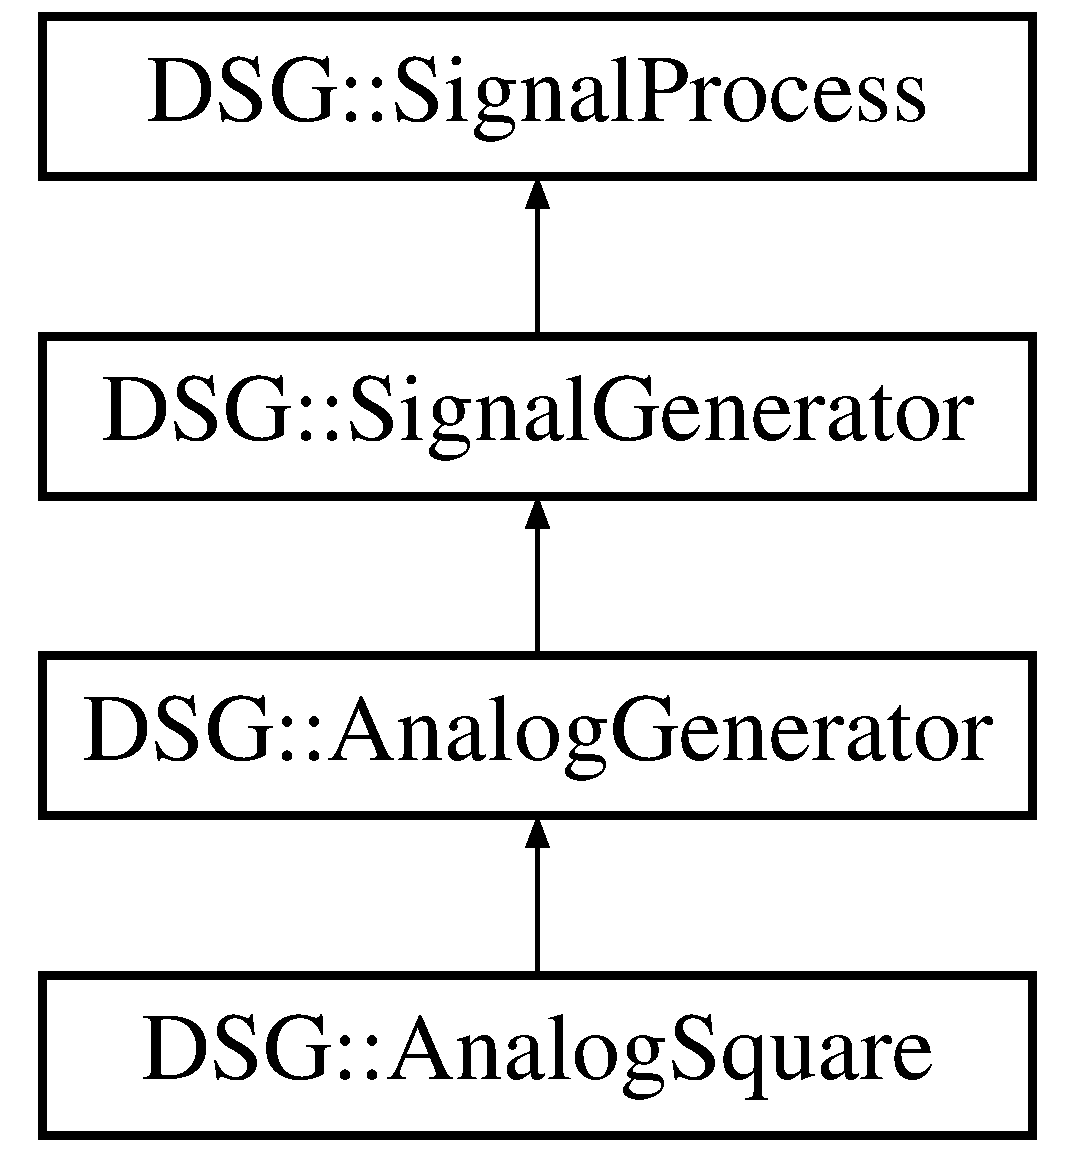
\includegraphics[height=4.000000cm]{classDSG_1_1AnalogSquare}
\end{center}
\end{figure}
\subsection*{Public Member Functions}
\begin{DoxyCompactItemize}
\item 
\hyperlink{classDSG_1_1AnalogSquare_a7b374bcd40345aec6a63e1789c2de732}{Analog\+Square} ()
\item 
\hyperlink{classDSG_1_1AnalogSquare_a80192f3cb9a8e6a31121de58b8c4b1ea}{Analog\+Square} (double const \&frequency, double const \&phase\+\_\+offset)
\item 
virtual \hyperlink{classDSG_1_1AnalogSquare_acece15975ff370006ecd985de3ad0ada}{$\sim$\+Analog\+Square} ()
\item 
virtual bool \hyperlink{classDSG_1_1AnalogSquare_a93a4b464545a32f72491d3df490fd3f7}{Perform} (\hyperlink{classDSG_1_1Sample}{Sample} \&signal)
\item 
virtual bool \hyperlink{classDSG_1_1AnalogSquare_a1d9c8a380775a7e4f6e0aa8fb1b05af6}{Perform} (\hyperlink{classDSG_1_1RingBuffer}{Ring\+Buffer} \&signal)
\item 
virtual bool \hyperlink{classDSG_1_1SignalProcess_afdb8220100418893950c1161dd24db67}{Perform} (\hyperlink{classDSG_1_1Sample_aaf2e30d73911eccea99b53eeee15b612}{Sample\+::\+Sample} \&signal)=0
\item 
virtual double const \& \hyperlink{classDSG_1_1SignalGenerator_aedac746c5a70818d120858542ecb7c45}{Frequency} () const 
\item 
virtual double const \& \hyperlink{classDSG_1_1SignalGenerator_ae3ce8d45bafabbd86a0f535b15c3cd46}{Frequency} (double const \&value)
\item 
virtual double const \& \hyperlink{classDSG_1_1SignalGenerator_a1ce521847edd0b837fd840998f906b4b}{Phase\+Offset} () const 
\item 
virtual double const \& \hyperlink{classDSG_1_1SignalGenerator_a08b71b1f30ba65e629642c570291dc0e}{Phase\+Offset} (double const \&value)
\end{DoxyCompactItemize}
\subsection*{Protected Member Functions}
\begin{DoxyCompactItemize}
\item 
double \hyperlink{classDSG_1_1SignalGenerator_ac0d781b8673b3a283bf7c133290ede50}{\+\_\+pstep} ()
\item 
double \hyperlink{classDSG_1_1SignalGenerator_ae660eb4caa88b8d278f8d24d0908a487}{\+\_\+pstep\+\_\+rad} ()
\item 
void \hyperlink{classDSG_1_1SignalGenerator_a05baccb38d1e52860d4fcf7cb8430efc}{\+\_\+psync} ()
\end{DoxyCompactItemize}
\subsection*{Protected Attributes}
\begin{DoxyCompactItemize}
\item 
double \hyperlink{classDSG_1_1AnalogSquare_a2bf2a892c6609816019771301f32b787}{\+\_\+duty}
\item 
\hyperlink{classDSG_1_1Sample}{Sample} \hyperlink{classDSG_1_1AnalogGenerator_ac88ad591cac37f636c2f7b460480bef9}{\+\_\+sample}
\item 
double \hyperlink{classDSG_1_1SignalGenerator_aa10f6c85d9adee901139ea7fb346f39d}{\+\_\+rate}
\item 
double \hyperlink{classDSG_1_1SignalGenerator_a67e296e3506dcdf09402c667cddff9ac}{\+\_\+frequency}
\item 
double \hyperlink{classDSG_1_1SignalGenerator_ac2271b582bf699275f077ecb642a8cd9}{\+\_\+phasor}
\end{DoxyCompactItemize}


\subsection{Detailed Description}


Definition at line 15 of file Analog\+Square.\+h.



\subsection{Constructor \& Destructor Documentation}
\hypertarget{classDSG_1_1AnalogSquare_a7b374bcd40345aec6a63e1789c2de732}{\index{D\+S\+G\+::\+Analog\+Square@{D\+S\+G\+::\+Analog\+Square}!Analog\+Square@{Analog\+Square}}
\index{Analog\+Square@{Analog\+Square}!D\+S\+G\+::\+Analog\+Square@{D\+S\+G\+::\+Analog\+Square}}
\subsubsection[{Analog\+Square}]{\setlength{\rightskip}{0pt plus 5cm}D\+S\+G\+::\+Analog\+Square\+::\+Analog\+Square (
\begin{DoxyParamCaption}
{}
\end{DoxyParamCaption}
)}}\label{classDSG_1_1AnalogSquare_a7b374bcd40345aec6a63e1789c2de732}


Definition at line 11 of file Analog\+Square.\+cpp.


\begin{DoxyCode}
11                              :\hyperlink{classDSG_1_1AnalogGenerator}{DSG::AnalogGenerator}(),\hyperlink{classDSG_1_1AnalogSquare_a2bf2a892c6609816019771301f32b787}{\_duty}(0.5)\{
12     
13 \}
\end{DoxyCode}
\hypertarget{classDSG_1_1AnalogSquare_a80192f3cb9a8e6a31121de58b8c4b1ea}{\index{D\+S\+G\+::\+Analog\+Square@{D\+S\+G\+::\+Analog\+Square}!Analog\+Square@{Analog\+Square}}
\index{Analog\+Square@{Analog\+Square}!D\+S\+G\+::\+Analog\+Square@{D\+S\+G\+::\+Analog\+Square}}
\subsubsection[{Analog\+Square}]{\setlength{\rightskip}{0pt plus 5cm}D\+S\+G\+::\+Analog\+Square\+::\+Analog\+Square (
\begin{DoxyParamCaption}
\item[{double const \&}]{frequency, }
\item[{double const \&}]{phase\+\_\+offset}
\end{DoxyParamCaption}
)}}\label{classDSG_1_1AnalogSquare_a80192f3cb9a8e6a31121de58b8c4b1ea}


Definition at line 14 of file Analog\+Square.\+cpp.


\begin{DoxyCode}
14                                                                                :
      \hyperlink{classDSG_1_1AnalogGenerator}{DSG::AnalogGenerator}(frequency,phase\_offset),\hyperlink{classDSG_1_1AnalogSquare_a2bf2a892c6609816019771301f32b787}{\_duty}(0.5)\{
15     
16 \}
\end{DoxyCode}
\hypertarget{classDSG_1_1AnalogSquare_acece15975ff370006ecd985de3ad0ada}{\index{D\+S\+G\+::\+Analog\+Square@{D\+S\+G\+::\+Analog\+Square}!````~Analog\+Square@{$\sim$\+Analog\+Square}}
\index{````~Analog\+Square@{$\sim$\+Analog\+Square}!D\+S\+G\+::\+Analog\+Square@{D\+S\+G\+::\+Analog\+Square}}
\subsubsection[{$\sim$\+Analog\+Square}]{\setlength{\rightskip}{0pt plus 5cm}D\+S\+G\+::\+Analog\+Square\+::$\sim$\+Analog\+Square (
\begin{DoxyParamCaption}
{}
\end{DoxyParamCaption}
)\hspace{0.3cm}{\ttfamily [virtual]}}}\label{classDSG_1_1AnalogSquare_acece15975ff370006ecd985de3ad0ada}


Definition at line 17 of file Analog\+Square.\+cpp.


\begin{DoxyCode}
17                               \{
18     
19 \}\end{DoxyCode}


\subsection{Member Function Documentation}
\hypertarget{classDSG_1_1SignalGenerator_ac0d781b8673b3a283bf7c133290ede50}{\index{D\+S\+G\+::\+Analog\+Square@{D\+S\+G\+::\+Analog\+Square}!\+\_\+pstep@{\+\_\+pstep}}
\index{\+\_\+pstep@{\+\_\+pstep}!D\+S\+G\+::\+Analog\+Square@{D\+S\+G\+::\+Analog\+Square}}
\subsubsection[{\+\_\+pstep}]{\setlength{\rightskip}{0pt plus 5cm}double D\+S\+G\+::\+Signal\+Generator\+::\+\_\+pstep (
\begin{DoxyParamCaption}
{}
\end{DoxyParamCaption}
)\hspace{0.3cm}{\ttfamily [inline]}, {\ttfamily [protected]}, {\ttfamily [inherited]}}}\label{classDSG_1_1SignalGenerator_ac0d781b8673b3a283bf7c133290ede50}


Definition at line 64 of file Signal\+Generator.\+h.


\begin{DoxyCode}
64                                          \{
65         value = \hyperlink{classDSG_1_1SignalGenerator_ac2271b582bf699275f077ecb642a8cd9}{\_phasor};
66         \hyperlink{classDSG_1_1SignalGenerator_ac2271b582bf699275f077ecb642a8cd9}{\_phasor}+=\hyperlink{classDSG_1_1SignalGenerator_aa10f6c85d9adee901139ea7fb346f39d}{\_rate};
67         \hyperlink{classDSG_1_1SignalGenerator_ac2271b582bf699275f077ecb642a8cd9}{\_phasor}>1?\hyperlink{classDSG_1_1SignalGenerator_ac2271b582bf699275f077ecb642a8cd9}{\_phasor}-=1:0;\textcolor{comment}{//cheaper cheaper %1}
68         \textcolor{comment}{//\_phasor -= (unsigned long)\_phasor;//cheaper %1}
69         \textcolor{keywordflow}{return} value;
70     \}
\end{DoxyCode}
\hypertarget{classDSG_1_1SignalGenerator_ae660eb4caa88b8d278f8d24d0908a487}{\index{D\+S\+G\+::\+Analog\+Square@{D\+S\+G\+::\+Analog\+Square}!\+\_\+pstep\+\_\+rad@{\+\_\+pstep\+\_\+rad}}
\index{\+\_\+pstep\+\_\+rad@{\+\_\+pstep\+\_\+rad}!D\+S\+G\+::\+Analog\+Square@{D\+S\+G\+::\+Analog\+Square}}
\subsubsection[{\+\_\+pstep\+\_\+rad}]{\setlength{\rightskip}{0pt plus 5cm}double D\+S\+G\+::\+Signal\+Generator\+::\+\_\+pstep\+\_\+rad (
\begin{DoxyParamCaption}
{}
\end{DoxyParamCaption}
)\hspace{0.3cm}{\ttfamily [inline]}, {\ttfamily [protected]}, {\ttfamily [inherited]}}}\label{classDSG_1_1SignalGenerator_ae660eb4caa88b8d278f8d24d0908a487}


Definition at line 71 of file Signal\+Generator.\+h.


\begin{DoxyCode}
71                                              \{
72         \textcolor{keywordflow}{return} \hyperlink{PI_8h_a4912c64aec0c943b7985db6cb61ff83a}{TWOPI} * \hyperlink{classDSG_1_1SignalGenerator_ac0d781b8673b3a283bf7c133290ede50}{\_pstep}();
73     \}
\end{DoxyCode}
\hypertarget{classDSG_1_1SignalGenerator_a05baccb38d1e52860d4fcf7cb8430efc}{\index{D\+S\+G\+::\+Analog\+Square@{D\+S\+G\+::\+Analog\+Square}!\+\_\+psync@{\+\_\+psync}}
\index{\+\_\+psync@{\+\_\+psync}!D\+S\+G\+::\+Analog\+Square@{D\+S\+G\+::\+Analog\+Square}}
\subsubsection[{\+\_\+psync}]{\setlength{\rightskip}{0pt plus 5cm}void D\+S\+G\+::\+Signal\+Generator\+::\+\_\+psync (
\begin{DoxyParamCaption}
{}
\end{DoxyParamCaption}
)\hspace{0.3cm}{\ttfamily [inline]}, {\ttfamily [protected]}, {\ttfamily [inherited]}}}\label{classDSG_1_1SignalGenerator_a05baccb38d1e52860d4fcf7cb8430efc}


Definition at line 74 of file Signal\+Generator.\+h.


\begin{DoxyCode}
74                                        \{
75         \hyperlink{classDSG_1_1SignalGenerator_ac2271b582bf699275f077ecb642a8cd9}{\_phasor} = \_phase\_offset;
76     \}
\end{DoxyCode}
\hypertarget{classDSG_1_1SignalGenerator_aedac746c5a70818d120858542ecb7c45}{\index{D\+S\+G\+::\+Analog\+Square@{D\+S\+G\+::\+Analog\+Square}!Frequency@{Frequency}}
\index{Frequency@{Frequency}!D\+S\+G\+::\+Analog\+Square@{D\+S\+G\+::\+Analog\+Square}}
\subsubsection[{Frequency}]{\setlength{\rightskip}{0pt plus 5cm}double const \& D\+S\+G\+::\+Signal\+Generator\+::\+Frequency (
\begin{DoxyParamCaption}
{}
\end{DoxyParamCaption}
) const\hspace{0.3cm}{\ttfamily [virtual]}, {\ttfamily [inherited]}}}\label{classDSG_1_1SignalGenerator_aedac746c5a70818d120858542ecb7c45}


Definition at line 16 of file Signal\+Generator.\+cpp.


\begin{DoxyCode}
16                                                 \{
17     \textcolor{keywordflow}{return} \hyperlink{classDSG_1_1SignalGenerator_a67e296e3506dcdf09402c667cddff9ac}{\_frequency};
18 \}
\end{DoxyCode}
\hypertarget{classDSG_1_1SignalGenerator_ae3ce8d45bafabbd86a0f535b15c3cd46}{\index{D\+S\+G\+::\+Analog\+Square@{D\+S\+G\+::\+Analog\+Square}!Frequency@{Frequency}}
\index{Frequency@{Frequency}!D\+S\+G\+::\+Analog\+Square@{D\+S\+G\+::\+Analog\+Square}}
\subsubsection[{Frequency}]{\setlength{\rightskip}{0pt plus 5cm}double const \& D\+S\+G\+::\+Signal\+Generator\+::\+Frequency (
\begin{DoxyParamCaption}
\item[{double const \&}]{value}
\end{DoxyParamCaption}
)\hspace{0.3cm}{\ttfamily [virtual]}, {\ttfamily [inherited]}}}\label{classDSG_1_1SignalGenerator_ae3ce8d45bafabbd86a0f535b15c3cd46}


Reimplemented in \hyperlink{classDSG_1_1BLIT_a67b698a54f37c361945cae3e137af76f}{D\+S\+G\+::\+B\+L\+I\+T}, \hyperlink{classDSG_1_1FourierSaw_a929602365c9b29f30f523fa07a29966e}{D\+S\+G\+::\+Fourier\+Saw}, \hyperlink{classDSG_1_1FourierSquare_a80f94eabad633e105cfa673fdee332d6}{D\+S\+G\+::\+Fourier\+Square}, and \hyperlink{classDSG_1_1FourierTriangle_aebb275eee9fb923636a8db5e4aa90b39}{D\+S\+G\+::\+Fourier\+Triangle}.



Definition at line 19 of file Signal\+Generator.\+cpp.


\begin{DoxyCode}
19                                                               \{
20     \hyperlink{classDSG_1_1SignalGenerator_a67e296e3506dcdf09402c667cddff9ac}{\_frequency} = value;
21     \hyperlink{classDSG_1_1SignalGenerator_aa10f6c85d9adee901139ea7fb346f39d}{\_rate} = \hyperlink{classDSG_1_1SignalGenerator_a67e296e3506dcdf09402c667cddff9ac}{\_frequency}/ \hyperlink{namespaceDSG_a0c5c3a251b3688398da18138c5efe4bf}{Sample\_Rate}();
22     \textcolor{keywordflow}{return} \hyperlink{classDSG_1_1SignalGenerator_a67e296e3506dcdf09402c667cddff9ac}{\_frequency};
23 \}
\end{DoxyCode}
\hypertarget{classDSG_1_1AnalogSquare_a93a4b464545a32f72491d3df490fd3f7}{\index{D\+S\+G\+::\+Analog\+Square@{D\+S\+G\+::\+Analog\+Square}!Perform@{Perform}}
\index{Perform@{Perform}!D\+S\+G\+::\+Analog\+Square@{D\+S\+G\+::\+Analog\+Square}}
\subsubsection[{Perform}]{\setlength{\rightskip}{0pt plus 5cm}bool D\+S\+G\+::\+Analog\+Square\+::\+Perform (
\begin{DoxyParamCaption}
\item[{{\bf Sample} \&}]{signal}
\end{DoxyParamCaption}
)\hspace{0.3cm}{\ttfamily [inline]}, {\ttfamily [virtual]}}}\label{classDSG_1_1AnalogSquare_a93a4b464545a32f72491d3df490fd3f7}


Reimplemented from \hyperlink{classDSG_1_1AnalogGenerator_ac50033964304239b514b7ee9d064bc75}{D\+S\+G\+::\+Analog\+Generator}.



Definition at line 28 of file Analog\+Square.\+h.


\begin{DoxyCode}
28                                                         \{
29             \textcolor{keywordtype}{double} value = \hyperlink{classDSG_1_1SignalGenerator_ac0d781b8673b3a283bf7c133290ede50}{\_pstep}();
30             value-=0.5;
31             value*=2.0;
32             signal = value>=\hyperlink{classDSG_1_1AnalogSquare_a2bf2a892c6609816019771301f32b787}{\_duty} ? -1.0: 1.0;
33             \textcolor{keywordflow}{return} \textcolor{keyword}{true};
34         \}
\end{DoxyCode}
\hypertarget{classDSG_1_1AnalogSquare_a1d9c8a380775a7e4f6e0aa8fb1b05af6}{\index{D\+S\+G\+::\+Analog\+Square@{D\+S\+G\+::\+Analog\+Square}!Perform@{Perform}}
\index{Perform@{Perform}!D\+S\+G\+::\+Analog\+Square@{D\+S\+G\+::\+Analog\+Square}}
\subsubsection[{Perform}]{\setlength{\rightskip}{0pt plus 5cm}bool D\+S\+G\+::\+Analog\+Square\+::\+Perform (
\begin{DoxyParamCaption}
\item[{{\bf Ring\+Buffer} \&}]{signal}
\end{DoxyParamCaption}
)\hspace{0.3cm}{\ttfamily [inline]}, {\ttfamily [virtual]}}}\label{classDSG_1_1AnalogSquare_a1d9c8a380775a7e4f6e0aa8fb1b05af6}


Reimplemented from \hyperlink{classDSG_1_1AnalogGenerator_a1b4f1d4af926fcc3e9571db7960c8706}{D\+S\+G\+::\+Analog\+Generator}.



Definition at line 35 of file Analog\+Square.\+h.


\begin{DoxyCode}
35                                                             \{
36             signal.Flush();
37             \textcolor{keywordflow}{while} (!signal.Full()) \{
38                 \textcolor{keywordflow}{if} (\hyperlink{classDSG_1_1AnalogSquare_a93a4b464545a32f72491d3df490fd3f7}{Perform}(\hyperlink{classDSG_1_1AnalogGenerator_ac88ad591cac37f636c2f7b460480bef9}{\_sample})) \{
39                     \textcolor{keywordflow}{if}(signal.Write(\hyperlink{classDSG_1_1AnalogGenerator_ac88ad591cac37f636c2f7b460480bef9}{\_sample}))\{
40                     \}\textcolor{keywordflow}{else} \textcolor{keywordflow}{return} \textcolor{keyword}{false};
41                 \}\textcolor{keywordflow}{else} \textcolor{keywordflow}{return} \textcolor{keyword}{false};
42             \}\textcolor{keywordflow}{return} \textcolor{keyword}{true};
43         \}
\end{DoxyCode}
\hypertarget{classDSG_1_1SignalProcess_afdb8220100418893950c1161dd24db67}{\index{D\+S\+G\+::\+Analog\+Square@{D\+S\+G\+::\+Analog\+Square}!Perform@{Perform}}
\index{Perform@{Perform}!D\+S\+G\+::\+Analog\+Square@{D\+S\+G\+::\+Analog\+Square}}
\subsubsection[{Perform}]{\setlength{\rightskip}{0pt plus 5cm}virtual bool D\+S\+G\+::\+Signal\+Process\+::\+Perform (
\begin{DoxyParamCaption}
\item[{{\bf Sample\+::\+Sample} \&}]{signal}
\end{DoxyParamCaption}
)\hspace{0.3cm}{\ttfamily [inline]}, {\ttfamily [pure virtual]}, {\ttfamily [inherited]}}}\label{classDSG_1_1SignalProcess_afdb8220100418893950c1161dd24db67}
\hypertarget{classDSG_1_1SignalGenerator_a1ce521847edd0b837fd840998f906b4b}{\index{D\+S\+G\+::\+Analog\+Square@{D\+S\+G\+::\+Analog\+Square}!Phase\+Offset@{Phase\+Offset}}
\index{Phase\+Offset@{Phase\+Offset}!D\+S\+G\+::\+Analog\+Square@{D\+S\+G\+::\+Analog\+Square}}
\subsubsection[{Phase\+Offset}]{\setlength{\rightskip}{0pt plus 5cm}double const \& D\+S\+G\+::\+Signal\+Generator\+::\+Phase\+Offset (
\begin{DoxyParamCaption}
{}
\end{DoxyParamCaption}
) const\hspace{0.3cm}{\ttfamily [virtual]}, {\ttfamily [inherited]}}}\label{classDSG_1_1SignalGenerator_a1ce521847edd0b837fd840998f906b4b}


Definition at line 24 of file Signal\+Generator.\+cpp.


\begin{DoxyCode}
24                                                   \{
25     \textcolor{keywordflow}{return} \_phase\_offset;
26 \}
\end{DoxyCode}
\hypertarget{classDSG_1_1SignalGenerator_a08b71b1f30ba65e629642c570291dc0e}{\index{D\+S\+G\+::\+Analog\+Square@{D\+S\+G\+::\+Analog\+Square}!Phase\+Offset@{Phase\+Offset}}
\index{Phase\+Offset@{Phase\+Offset}!D\+S\+G\+::\+Analog\+Square@{D\+S\+G\+::\+Analog\+Square}}
\subsubsection[{Phase\+Offset}]{\setlength{\rightskip}{0pt plus 5cm}double const \& D\+S\+G\+::\+Signal\+Generator\+::\+Phase\+Offset (
\begin{DoxyParamCaption}
\item[{double const \&}]{value}
\end{DoxyParamCaption}
)\hspace{0.3cm}{\ttfamily [virtual]}, {\ttfamily [inherited]}}}\label{classDSG_1_1SignalGenerator_a08b71b1f30ba65e629642c570291dc0e}


Definition at line 27 of file Signal\+Generator.\+cpp.


\begin{DoxyCode}
27                                                                 \{
28     \_phase\_offset-=value;
29     \hyperlink{classDSG_1_1SignalGenerator_ac2271b582bf699275f077ecb642a8cd9}{\_phasor}-=\_phase\_offset;
30     \_phase\_offset=value;
31     \textcolor{keywordflow}{return} \_phase\_offset;
32 \}
\end{DoxyCode}


\subsection{Member Data Documentation}
\hypertarget{classDSG_1_1AnalogSquare_a2bf2a892c6609816019771301f32b787}{\index{D\+S\+G\+::\+Analog\+Square@{D\+S\+G\+::\+Analog\+Square}!\+\_\+duty@{\+\_\+duty}}
\index{\+\_\+duty@{\+\_\+duty}!D\+S\+G\+::\+Analog\+Square@{D\+S\+G\+::\+Analog\+Square}}
\subsubsection[{\+\_\+duty}]{\setlength{\rightskip}{0pt plus 5cm}double D\+S\+G\+::\+Analog\+Square\+::\+\_\+duty\hspace{0.3cm}{\ttfamily [protected]}}}\label{classDSG_1_1AnalogSquare_a2bf2a892c6609816019771301f32b787}


Definition at line 24 of file Analog\+Square.\+h.

\hypertarget{classDSG_1_1SignalGenerator_a67e296e3506dcdf09402c667cddff9ac}{\index{D\+S\+G\+::\+Analog\+Square@{D\+S\+G\+::\+Analog\+Square}!\+\_\+frequency@{\+\_\+frequency}}
\index{\+\_\+frequency@{\+\_\+frequency}!D\+S\+G\+::\+Analog\+Square@{D\+S\+G\+::\+Analog\+Square}}
\subsubsection[{\+\_\+frequency}]{\setlength{\rightskip}{0pt plus 5cm}double D\+S\+G\+::\+Signal\+Generator\+::\+\_\+frequency\hspace{0.3cm}{\ttfamily [protected]}, {\ttfamily [inherited]}}}\label{classDSG_1_1SignalGenerator_a67e296e3506dcdf09402c667cddff9ac}


Definition at line 34 of file Signal\+Generator.\+h.

\hypertarget{classDSG_1_1SignalGenerator_ac2271b582bf699275f077ecb642a8cd9}{\index{D\+S\+G\+::\+Analog\+Square@{D\+S\+G\+::\+Analog\+Square}!\+\_\+phasor@{\+\_\+phasor}}
\index{\+\_\+phasor@{\+\_\+phasor}!D\+S\+G\+::\+Analog\+Square@{D\+S\+G\+::\+Analog\+Square}}
\subsubsection[{\+\_\+phasor}]{\setlength{\rightskip}{0pt plus 5cm}double D\+S\+G\+::\+Signal\+Generator\+::\+\_\+phasor\hspace{0.3cm}{\ttfamily [protected]}, {\ttfamily [inherited]}}}\label{classDSG_1_1SignalGenerator_ac2271b582bf699275f077ecb642a8cd9}


Definition at line 46 of file Signal\+Generator.\+h.

\hypertarget{classDSG_1_1SignalGenerator_aa10f6c85d9adee901139ea7fb346f39d}{\index{D\+S\+G\+::\+Analog\+Square@{D\+S\+G\+::\+Analog\+Square}!\+\_\+rate@{\+\_\+rate}}
\index{\+\_\+rate@{\+\_\+rate}!D\+S\+G\+::\+Analog\+Square@{D\+S\+G\+::\+Analog\+Square}}
\subsubsection[{\+\_\+rate}]{\setlength{\rightskip}{0pt plus 5cm}double D\+S\+G\+::\+Signal\+Generator\+::\+\_\+rate\hspace{0.3cm}{\ttfamily [protected]}, {\ttfamily [inherited]}}}\label{classDSG_1_1SignalGenerator_aa10f6c85d9adee901139ea7fb346f39d}


Definition at line 33 of file Signal\+Generator.\+h.

\hypertarget{classDSG_1_1AnalogGenerator_ac88ad591cac37f636c2f7b460480bef9}{\index{D\+S\+G\+::\+Analog\+Square@{D\+S\+G\+::\+Analog\+Square}!\+\_\+sample@{\+\_\+sample}}
\index{\+\_\+sample@{\+\_\+sample}!D\+S\+G\+::\+Analog\+Square@{D\+S\+G\+::\+Analog\+Square}}
\subsubsection[{\+\_\+sample}]{\setlength{\rightskip}{0pt plus 5cm}{\bf Sample} D\+S\+G\+::\+Analog\+Generator\+::\+\_\+sample\hspace{0.3cm}{\ttfamily [protected]}, {\ttfamily [inherited]}}}\label{classDSG_1_1AnalogGenerator_ac88ad591cac37f636c2f7b460480bef9}


Definition at line 28 of file Analog\+Generator.\+h.



The documentation for this class was generated from the following files\+:\begin{DoxyCompactItemize}
\item 
/\+Users/alexanderzywicki/\+Documents/\+School\+\_\+\+Stuff/\+Fall\+\_\+2014/\+Digital\+\_\+\+Signal\+\_\+\+Generation\+\_\+and\+\_\+\+Analysis/src/include/\hyperlink{AnalogSquare_8h}{Analog\+Square.\+h}\item 
/\+Users/alexanderzywicki/\+Documents/\+School\+\_\+\+Stuff/\+Fall\+\_\+2014/\+Digital\+\_\+\+Signal\+\_\+\+Generation\+\_\+and\+\_\+\+Analysis/src/\hyperlink{AnalogSquare_8cpp}{Analog\+Square.\+cpp}\end{DoxyCompactItemize}

\hypertarget{classDSG_1_1AnalogTriangle}{\section{D\+S\+G\+:\+:Analog\+Triangle Class Reference}
\label{classDSG_1_1AnalogTriangle}\index{D\+S\+G\+::\+Analog\+Triangle@{D\+S\+G\+::\+Analog\+Triangle}}
}


{\ttfamily \#include $<$Analog\+Triangle.\+h$>$}

Inheritance diagram for D\+S\+G\+:\+:Analog\+Triangle\+:\begin{figure}[H]
\begin{center}
\leavevmode
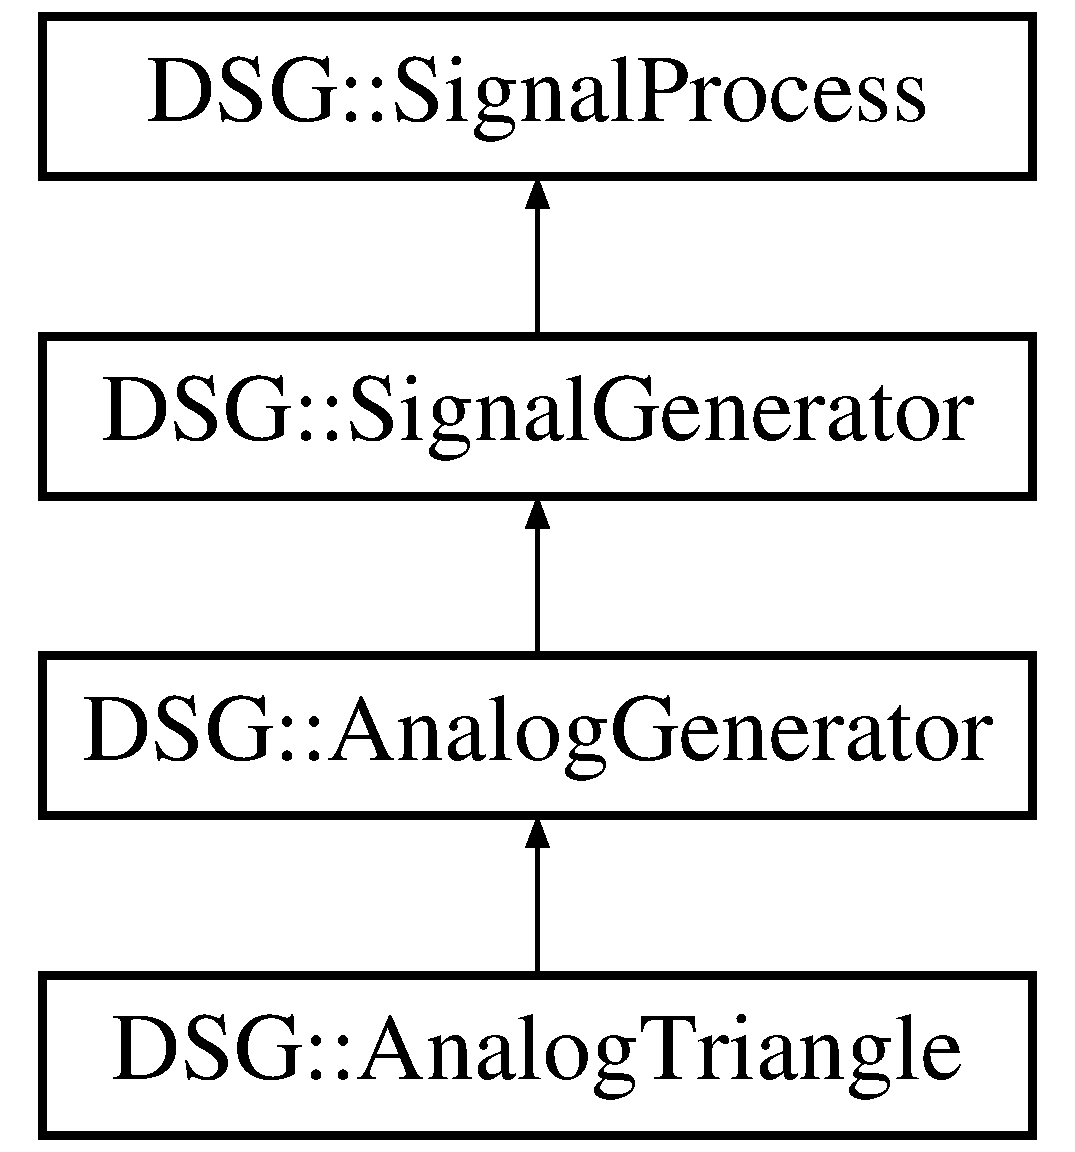
\includegraphics[height=4.000000cm]{classDSG_1_1AnalogTriangle}
\end{center}
\end{figure}
\subsection*{Public Member Functions}
\begin{DoxyCompactItemize}
\item 
\hyperlink{classDSG_1_1AnalogTriangle_a42f8f20b211eb758b5b9acd4384308e2}{Analog\+Triangle} ()
\item 
\hyperlink{classDSG_1_1AnalogTriangle_aa677150201428cd206391367672454e7}{Analog\+Triangle} (double const \&frequency, double const \&phase\+\_\+offset)
\item 
virtual \hyperlink{classDSG_1_1AnalogTriangle_a9b5ed8f1759b53827b398859776210fc}{$\sim$\+Analog\+Triangle} ()
\item 
virtual bool \hyperlink{classDSG_1_1AnalogTriangle_ac3edb87c395763d6894672b471850b05}{Perform} (\hyperlink{classDSG_1_1Sample}{Sample} \&signal)
\item 
virtual bool \hyperlink{classDSG_1_1AnalogTriangle_a9456183af28d98ccf3daa85b8ad12b52}{Perform} (\hyperlink{classDSG_1_1RingBuffer}{Ring\+Buffer} \&signal)
\item 
virtual bool \hyperlink{classDSG_1_1SignalProcess_afdb8220100418893950c1161dd24db67}{Perform} (\hyperlink{classDSG_1_1Sample_aaf2e30d73911eccea99b53eeee15b612}{Sample\+::\+Sample} \&signal)=0
\item 
virtual double const \& \hyperlink{classDSG_1_1SignalGenerator_aedac746c5a70818d120858542ecb7c45}{Frequency} () const 
\item 
virtual double const \& \hyperlink{classDSG_1_1SignalGenerator_ae3ce8d45bafabbd86a0f535b15c3cd46}{Frequency} (double const \&value)
\item 
virtual double const \& \hyperlink{classDSG_1_1SignalGenerator_a1ce521847edd0b837fd840998f906b4b}{Phase\+Offset} () const 
\item 
virtual double const \& \hyperlink{classDSG_1_1SignalGenerator_a08b71b1f30ba65e629642c570291dc0e}{Phase\+Offset} (double const \&value)
\end{DoxyCompactItemize}
\subsection*{Protected Member Functions}
\begin{DoxyCompactItemize}
\item 
double \hyperlink{classDSG_1_1SignalGenerator_ac0d781b8673b3a283bf7c133290ede50}{\+\_\+pstep} ()
\item 
double \hyperlink{classDSG_1_1SignalGenerator_ae660eb4caa88b8d278f8d24d0908a487}{\+\_\+pstep\+\_\+rad} ()
\item 
void \hyperlink{classDSG_1_1SignalGenerator_a05baccb38d1e52860d4fcf7cb8430efc}{\+\_\+psync} ()
\end{DoxyCompactItemize}
\subsection*{Protected Attributes}
\begin{DoxyCompactItemize}
\item 
\hyperlink{classDSG_1_1Sample}{Sample} \hyperlink{classDSG_1_1AnalogGenerator_ac88ad591cac37f636c2f7b460480bef9}{\+\_\+sample}
\item 
double \hyperlink{classDSG_1_1SignalGenerator_aa10f6c85d9adee901139ea7fb346f39d}{\+\_\+rate}
\item 
double \hyperlink{classDSG_1_1SignalGenerator_a67e296e3506dcdf09402c667cddff9ac}{\+\_\+frequency}
\item 
double \hyperlink{classDSG_1_1SignalGenerator_ac2271b582bf699275f077ecb642a8cd9}{\+\_\+phasor}
\end{DoxyCompactItemize}


\subsection{Detailed Description}


Definition at line 14 of file Analog\+Triangle.\+h.



\subsection{Constructor \& Destructor Documentation}
\hypertarget{classDSG_1_1AnalogTriangle_a42f8f20b211eb758b5b9acd4384308e2}{\index{D\+S\+G\+::\+Analog\+Triangle@{D\+S\+G\+::\+Analog\+Triangle}!Analog\+Triangle@{Analog\+Triangle}}
\index{Analog\+Triangle@{Analog\+Triangle}!D\+S\+G\+::\+Analog\+Triangle@{D\+S\+G\+::\+Analog\+Triangle}}
\subsubsection[{Analog\+Triangle}]{\setlength{\rightskip}{0pt plus 5cm}D\+S\+G\+::\+Analog\+Triangle\+::\+Analog\+Triangle (
\begin{DoxyParamCaption}
{}
\end{DoxyParamCaption}
)}}\label{classDSG_1_1AnalogTriangle_a42f8f20b211eb758b5b9acd4384308e2}


Definition at line 9 of file Analog\+Triangle.\+cpp.


\begin{DoxyCode}
9 :\hyperlink{classDSG_1_1AnalogGenerator}{DSG::AnalogGenerator}()\{\}
\end{DoxyCode}
\hypertarget{classDSG_1_1AnalogTriangle_aa677150201428cd206391367672454e7}{\index{D\+S\+G\+::\+Analog\+Triangle@{D\+S\+G\+::\+Analog\+Triangle}!Analog\+Triangle@{Analog\+Triangle}}
\index{Analog\+Triangle@{Analog\+Triangle}!D\+S\+G\+::\+Analog\+Triangle@{D\+S\+G\+::\+Analog\+Triangle}}
\subsubsection[{Analog\+Triangle}]{\setlength{\rightskip}{0pt plus 5cm}D\+S\+G\+::\+Analog\+Triangle\+::\+Analog\+Triangle (
\begin{DoxyParamCaption}
\item[{double const \&}]{frequency, }
\item[{double const \&}]{phase\+\_\+offset}
\end{DoxyParamCaption}
)}}\label{classDSG_1_1AnalogTriangle_aa677150201428cd206391367672454e7}


Definition at line 10 of file Analog\+Triangle.\+cpp.


\begin{DoxyCode}
10 :\hyperlink{classDSG_1_1AnalogGenerator}{DSG::AnalogGenerator}(frequency,phase\_offset)\{\}
\end{DoxyCode}
\hypertarget{classDSG_1_1AnalogTriangle_a9b5ed8f1759b53827b398859776210fc}{\index{D\+S\+G\+::\+Analog\+Triangle@{D\+S\+G\+::\+Analog\+Triangle}!````~Analog\+Triangle@{$\sim$\+Analog\+Triangle}}
\index{````~Analog\+Triangle@{$\sim$\+Analog\+Triangle}!D\+S\+G\+::\+Analog\+Triangle@{D\+S\+G\+::\+Analog\+Triangle}}
\subsubsection[{$\sim$\+Analog\+Triangle}]{\setlength{\rightskip}{0pt plus 5cm}D\+S\+G\+::\+Analog\+Triangle\+::$\sim$\+Analog\+Triangle (
\begin{DoxyParamCaption}
{}
\end{DoxyParamCaption}
)\hspace{0.3cm}{\ttfamily [virtual]}}}\label{classDSG_1_1AnalogTriangle_a9b5ed8f1759b53827b398859776210fc}


Definition at line 11 of file Analog\+Triangle.\+cpp.


\begin{DoxyCode}
11 \{\}\end{DoxyCode}


\subsection{Member Function Documentation}
\hypertarget{classDSG_1_1SignalGenerator_ac0d781b8673b3a283bf7c133290ede50}{\index{D\+S\+G\+::\+Analog\+Triangle@{D\+S\+G\+::\+Analog\+Triangle}!\+\_\+pstep@{\+\_\+pstep}}
\index{\+\_\+pstep@{\+\_\+pstep}!D\+S\+G\+::\+Analog\+Triangle@{D\+S\+G\+::\+Analog\+Triangle}}
\subsubsection[{\+\_\+pstep}]{\setlength{\rightskip}{0pt plus 5cm}double D\+S\+G\+::\+Signal\+Generator\+::\+\_\+pstep (
\begin{DoxyParamCaption}
{}
\end{DoxyParamCaption}
)\hspace{0.3cm}{\ttfamily [inline]}, {\ttfamily [protected]}, {\ttfamily [inherited]}}}\label{classDSG_1_1SignalGenerator_ac0d781b8673b3a283bf7c133290ede50}


Definition at line 52 of file Signal\+Generator.\+h.


\begin{DoxyCode}
52                                          \{
53         value = \hyperlink{classDSG_1_1SignalGenerator_ac2271b582bf699275f077ecb642a8cd9}{\_phasor};
54         \hyperlink{classDSG_1_1SignalGenerator_ac2271b582bf699275f077ecb642a8cd9}{\_phasor}+=\hyperlink{classDSG_1_1SignalGenerator_aa10f6c85d9adee901139ea7fb346f39d}{\_rate};
55         \hyperlink{classDSG_1_1SignalGenerator_ac2271b582bf699275f077ecb642a8cd9}{\_phasor}>1?\hyperlink{classDSG_1_1SignalGenerator_ac2271b582bf699275f077ecb642a8cd9}{\_phasor}-=1:0;\textcolor{comment}{//cheaper cheaper %1}
56         \textcolor{comment}{//\_phasor -= (unsigned long)\_phasor;//cheaper %1}
57         \textcolor{keywordflow}{return} value;
58     \}
\end{DoxyCode}
\hypertarget{classDSG_1_1SignalGenerator_ae660eb4caa88b8d278f8d24d0908a487}{\index{D\+S\+G\+::\+Analog\+Triangle@{D\+S\+G\+::\+Analog\+Triangle}!\+\_\+pstep\+\_\+rad@{\+\_\+pstep\+\_\+rad}}
\index{\+\_\+pstep\+\_\+rad@{\+\_\+pstep\+\_\+rad}!D\+S\+G\+::\+Analog\+Triangle@{D\+S\+G\+::\+Analog\+Triangle}}
\subsubsection[{\+\_\+pstep\+\_\+rad}]{\setlength{\rightskip}{0pt plus 5cm}double D\+S\+G\+::\+Signal\+Generator\+::\+\_\+pstep\+\_\+rad (
\begin{DoxyParamCaption}
{}
\end{DoxyParamCaption}
)\hspace{0.3cm}{\ttfamily [inline]}, {\ttfamily [protected]}, {\ttfamily [inherited]}}}\label{classDSG_1_1SignalGenerator_ae660eb4caa88b8d278f8d24d0908a487}


Definition at line 59 of file Signal\+Generator.\+h.


\begin{DoxyCode}
59                                              \{
60         \textcolor{keywordflow}{return} \hyperlink{PI_8h_a4912c64aec0c943b7985db6cb61ff83a}{TWOPI} * \hyperlink{classDSG_1_1SignalGenerator_ac0d781b8673b3a283bf7c133290ede50}{\_pstep}();
61     \}
\end{DoxyCode}
\hypertarget{classDSG_1_1SignalGenerator_a05baccb38d1e52860d4fcf7cb8430efc}{\index{D\+S\+G\+::\+Analog\+Triangle@{D\+S\+G\+::\+Analog\+Triangle}!\+\_\+psync@{\+\_\+psync}}
\index{\+\_\+psync@{\+\_\+psync}!D\+S\+G\+::\+Analog\+Triangle@{D\+S\+G\+::\+Analog\+Triangle}}
\subsubsection[{\+\_\+psync}]{\setlength{\rightskip}{0pt plus 5cm}void D\+S\+G\+::\+Signal\+Generator\+::\+\_\+psync (
\begin{DoxyParamCaption}
{}
\end{DoxyParamCaption}
)\hspace{0.3cm}{\ttfamily [inline]}, {\ttfamily [protected]}, {\ttfamily [inherited]}}}\label{classDSG_1_1SignalGenerator_a05baccb38d1e52860d4fcf7cb8430efc}


Definition at line 62 of file Signal\+Generator.\+h.


\begin{DoxyCode}
62                                        \{
63         \hyperlink{classDSG_1_1SignalGenerator_ac2271b582bf699275f077ecb642a8cd9}{\_phasor} = \_phase\_offset;
64     \}
\end{DoxyCode}
\hypertarget{classDSG_1_1SignalGenerator_aedac746c5a70818d120858542ecb7c45}{\index{D\+S\+G\+::\+Analog\+Triangle@{D\+S\+G\+::\+Analog\+Triangle}!Frequency@{Frequency}}
\index{Frequency@{Frequency}!D\+S\+G\+::\+Analog\+Triangle@{D\+S\+G\+::\+Analog\+Triangle}}
\subsubsection[{Frequency}]{\setlength{\rightskip}{0pt plus 5cm}double const \& D\+S\+G\+::\+Signal\+Generator\+::\+Frequency (
\begin{DoxyParamCaption}
{}
\end{DoxyParamCaption}
) const\hspace{0.3cm}{\ttfamily [virtual]}, {\ttfamily [inherited]}}}\label{classDSG_1_1SignalGenerator_aedac746c5a70818d120858542ecb7c45}


Definition at line 14 of file Signal\+Generator.\+cpp.


\begin{DoxyCode}
14                                                 \{
15     \textcolor{keywordflow}{return} \hyperlink{classDSG_1_1SignalGenerator_a67e296e3506dcdf09402c667cddff9ac}{\_frequency};
16 \}
\end{DoxyCode}
\hypertarget{classDSG_1_1SignalGenerator_ae3ce8d45bafabbd86a0f535b15c3cd46}{\index{D\+S\+G\+::\+Analog\+Triangle@{D\+S\+G\+::\+Analog\+Triangle}!Frequency@{Frequency}}
\index{Frequency@{Frequency}!D\+S\+G\+::\+Analog\+Triangle@{D\+S\+G\+::\+Analog\+Triangle}}
\subsubsection[{Frequency}]{\setlength{\rightskip}{0pt plus 5cm}double const \& D\+S\+G\+::\+Signal\+Generator\+::\+Frequency (
\begin{DoxyParamCaption}
\item[{double const \&}]{value}
\end{DoxyParamCaption}
)\hspace{0.3cm}{\ttfamily [virtual]}, {\ttfamily [inherited]}}}\label{classDSG_1_1SignalGenerator_ae3ce8d45bafabbd86a0f535b15c3cd46}


Reimplemented in \hyperlink{classDSG_1_1BLIT_a67b698a54f37c361945cae3e137af76f}{D\+S\+G\+::\+B\+L\+I\+T}, \hyperlink{classDSG_1_1FourierTriangle_aebb275eee9fb923636a8db5e4aa90b39}{D\+S\+G\+::\+Fourier\+Triangle}, \hyperlink{classDSG_1_1FourierSaw_a929602365c9b29f30f523fa07a29966e}{D\+S\+G\+::\+Fourier\+Saw}, and \hyperlink{classDSG_1_1FourierSquare_a80f94eabad633e105cfa673fdee332d6}{D\+S\+G\+::\+Fourier\+Square}.



Definition at line 17 of file Signal\+Generator.\+cpp.


\begin{DoxyCode}
17                                                               \{
18     \hyperlink{classDSG_1_1SignalGenerator_a67e296e3506dcdf09402c667cddff9ac}{\_frequency} = value;
19     \hyperlink{classDSG_1_1SignalGenerator_aa10f6c85d9adee901139ea7fb346f39d}{\_rate} = \hyperlink{classDSG_1_1SignalGenerator_a67e296e3506dcdf09402c667cddff9ac}{\_frequency}/ \hyperlink{namespaceDSG_a0c5c3a251b3688398da18138c5efe4bf}{Sample\_Rate}();
20     \textcolor{keywordflow}{return} \hyperlink{classDSG_1_1SignalGenerator_a67e296e3506dcdf09402c667cddff9ac}{\_frequency};
21 \}
\end{DoxyCode}
\hypertarget{classDSG_1_1AnalogTriangle_ac3edb87c395763d6894672b471850b05}{\index{D\+S\+G\+::\+Analog\+Triangle@{D\+S\+G\+::\+Analog\+Triangle}!Perform@{Perform}}
\index{Perform@{Perform}!D\+S\+G\+::\+Analog\+Triangle@{D\+S\+G\+::\+Analog\+Triangle}}
\subsubsection[{Perform}]{\setlength{\rightskip}{0pt plus 5cm}bool D\+S\+G\+::\+Analog\+Triangle\+::\+Perform (
\begin{DoxyParamCaption}
\item[{{\bf Sample} \&}]{signal}
\end{DoxyParamCaption}
)\hspace{0.3cm}{\ttfamily [inline]}, {\ttfamily [virtual]}}}\label{classDSG_1_1AnalogTriangle_ac3edb87c395763d6894672b471850b05}


Reimplemented from \hyperlink{classDSG_1_1AnalogGenerator_ac50033964304239b514b7ee9d064bc75}{D\+S\+G\+::\+Analog\+Generator}.



Definition at line 24 of file Analog\+Triangle.\+h.


\begin{DoxyCode}
24                                                       \{
25         \textcolor{keywordtype}{double} value = \hyperlink{classDSG_1_1SignalGenerator_ac0d781b8673b3a283bf7c133290ede50}{\_pstep}();
26         
27         value+=0.25;
28         value-=(long)value;
29         value-=0.5;
30         value*=2.0;
31         value = value <0.0 ?  value: -1*value;
32         value+=0.5;
33         value*=2.0;
34         signal = value;
35         \textcolor{keywordflow}{return} \textcolor{keyword}{true};
36     \}
\end{DoxyCode}
\hypertarget{classDSG_1_1SignalProcess_afdb8220100418893950c1161dd24db67}{\index{D\+S\+G\+::\+Analog\+Triangle@{D\+S\+G\+::\+Analog\+Triangle}!Perform@{Perform}}
\index{Perform@{Perform}!D\+S\+G\+::\+Analog\+Triangle@{D\+S\+G\+::\+Analog\+Triangle}}
\subsubsection[{Perform}]{\setlength{\rightskip}{0pt plus 5cm}virtual bool D\+S\+G\+::\+Signal\+Process\+::\+Perform (
\begin{DoxyParamCaption}
\item[{{\bf Sample\+::\+Sample} \&}]{signal}
\end{DoxyParamCaption}
)\hspace{0.3cm}{\ttfamily [inline]}, {\ttfamily [pure virtual]}, {\ttfamily [inherited]}}}\label{classDSG_1_1SignalProcess_afdb8220100418893950c1161dd24db67}
\hypertarget{classDSG_1_1AnalogTriangle_a9456183af28d98ccf3daa85b8ad12b52}{\index{D\+S\+G\+::\+Analog\+Triangle@{D\+S\+G\+::\+Analog\+Triangle}!Perform@{Perform}}
\index{Perform@{Perform}!D\+S\+G\+::\+Analog\+Triangle@{D\+S\+G\+::\+Analog\+Triangle}}
\subsubsection[{Perform}]{\setlength{\rightskip}{0pt plus 5cm}bool D\+S\+G\+::\+Analog\+Triangle\+::\+Perform (
\begin{DoxyParamCaption}
\item[{{\bf Ring\+Buffer} \&}]{signal}
\end{DoxyParamCaption}
)\hspace{0.3cm}{\ttfamily [inline]}, {\ttfamily [virtual]}}}\label{classDSG_1_1AnalogTriangle_a9456183af28d98ccf3daa85b8ad12b52}


Reimplemented from \hyperlink{classDSG_1_1AnalogGenerator_a1b4f1d4af926fcc3e9571db7960c8706}{D\+S\+G\+::\+Analog\+Generator}.



Definition at line 37 of file Analog\+Triangle.\+h.


\begin{DoxyCode}
37                                                           \{
38         signal.Flush();
39         \textcolor{keywordflow}{while} (!signal.Full()) \{
40             \textcolor{keywordflow}{if} (\hyperlink{classDSG_1_1AnalogTriangle_ac3edb87c395763d6894672b471850b05}{Perform}(\hyperlink{classDSG_1_1AnalogGenerator_ac88ad591cac37f636c2f7b460480bef9}{\_sample})) \{
41                 \textcolor{keywordflow}{if}(signal.Write(\hyperlink{classDSG_1_1AnalogGenerator_ac88ad591cac37f636c2f7b460480bef9}{\_sample}))\{
42                 \}\textcolor{keywordflow}{else} \textcolor{keywordflow}{return} \textcolor{keyword}{false};
43             \}\textcolor{keywordflow}{else} \textcolor{keywordflow}{return} \textcolor{keyword}{false};
44         \}\textcolor{keywordflow}{return} \textcolor{keyword}{true};
45     \}
\end{DoxyCode}
\hypertarget{classDSG_1_1SignalGenerator_a1ce521847edd0b837fd840998f906b4b}{\index{D\+S\+G\+::\+Analog\+Triangle@{D\+S\+G\+::\+Analog\+Triangle}!Phase\+Offset@{Phase\+Offset}}
\index{Phase\+Offset@{Phase\+Offset}!D\+S\+G\+::\+Analog\+Triangle@{D\+S\+G\+::\+Analog\+Triangle}}
\subsubsection[{Phase\+Offset}]{\setlength{\rightskip}{0pt plus 5cm}double const \& D\+S\+G\+::\+Signal\+Generator\+::\+Phase\+Offset (
\begin{DoxyParamCaption}
{}
\end{DoxyParamCaption}
) const\hspace{0.3cm}{\ttfamily [virtual]}, {\ttfamily [inherited]}}}\label{classDSG_1_1SignalGenerator_a1ce521847edd0b837fd840998f906b4b}


Definition at line 22 of file Signal\+Generator.\+cpp.


\begin{DoxyCode}
22                                                   \{
23     \textcolor{keywordflow}{return} \_phase\_offset;
24 \}
\end{DoxyCode}
\hypertarget{classDSG_1_1SignalGenerator_a08b71b1f30ba65e629642c570291dc0e}{\index{D\+S\+G\+::\+Analog\+Triangle@{D\+S\+G\+::\+Analog\+Triangle}!Phase\+Offset@{Phase\+Offset}}
\index{Phase\+Offset@{Phase\+Offset}!D\+S\+G\+::\+Analog\+Triangle@{D\+S\+G\+::\+Analog\+Triangle}}
\subsubsection[{Phase\+Offset}]{\setlength{\rightskip}{0pt plus 5cm}double const \& D\+S\+G\+::\+Signal\+Generator\+::\+Phase\+Offset (
\begin{DoxyParamCaption}
\item[{double const \&}]{value}
\end{DoxyParamCaption}
)\hspace{0.3cm}{\ttfamily [virtual]}, {\ttfamily [inherited]}}}\label{classDSG_1_1SignalGenerator_a08b71b1f30ba65e629642c570291dc0e}


Definition at line 25 of file Signal\+Generator.\+cpp.


\begin{DoxyCode}
25                                                                 \{
26     \_phase\_offset-=value;
27     \hyperlink{classDSG_1_1SignalGenerator_ac2271b582bf699275f077ecb642a8cd9}{\_phasor}-=\_phase\_offset;
28     \_phase\_offset=value;
29     \textcolor{keywordflow}{return} \_phase\_offset;
30 \}\end{DoxyCode}


\subsection{Member Data Documentation}
\hypertarget{classDSG_1_1SignalGenerator_a67e296e3506dcdf09402c667cddff9ac}{\index{D\+S\+G\+::\+Analog\+Triangle@{D\+S\+G\+::\+Analog\+Triangle}!\+\_\+frequency@{\+\_\+frequency}}
\index{\+\_\+frequency@{\+\_\+frequency}!D\+S\+G\+::\+Analog\+Triangle@{D\+S\+G\+::\+Analog\+Triangle}}
\subsubsection[{\+\_\+frequency}]{\setlength{\rightskip}{0pt plus 5cm}double D\+S\+G\+::\+Signal\+Generator\+::\+\_\+frequency\hspace{0.3cm}{\ttfamily [protected]}, {\ttfamily [inherited]}}}\label{classDSG_1_1SignalGenerator_a67e296e3506dcdf09402c667cddff9ac}


Definition at line 28 of file Signal\+Generator.\+h.

\hypertarget{classDSG_1_1SignalGenerator_ac2271b582bf699275f077ecb642a8cd9}{\index{D\+S\+G\+::\+Analog\+Triangle@{D\+S\+G\+::\+Analog\+Triangle}!\+\_\+phasor@{\+\_\+phasor}}
\index{\+\_\+phasor@{\+\_\+phasor}!D\+S\+G\+::\+Analog\+Triangle@{D\+S\+G\+::\+Analog\+Triangle}}
\subsubsection[{\+\_\+phasor}]{\setlength{\rightskip}{0pt plus 5cm}double D\+S\+G\+::\+Signal\+Generator\+::\+\_\+phasor\hspace{0.3cm}{\ttfamily [protected]}, {\ttfamily [inherited]}}}\label{classDSG_1_1SignalGenerator_ac2271b582bf699275f077ecb642a8cd9}


Definition at line 38 of file Signal\+Generator.\+h.

\hypertarget{classDSG_1_1SignalGenerator_aa10f6c85d9adee901139ea7fb346f39d}{\index{D\+S\+G\+::\+Analog\+Triangle@{D\+S\+G\+::\+Analog\+Triangle}!\+\_\+rate@{\+\_\+rate}}
\index{\+\_\+rate@{\+\_\+rate}!D\+S\+G\+::\+Analog\+Triangle@{D\+S\+G\+::\+Analog\+Triangle}}
\subsubsection[{\+\_\+rate}]{\setlength{\rightskip}{0pt plus 5cm}double D\+S\+G\+::\+Signal\+Generator\+::\+\_\+rate\hspace{0.3cm}{\ttfamily [protected]}, {\ttfamily [inherited]}}}\label{classDSG_1_1SignalGenerator_aa10f6c85d9adee901139ea7fb346f39d}


Definition at line 27 of file Signal\+Generator.\+h.

\hypertarget{classDSG_1_1AnalogGenerator_ac88ad591cac37f636c2f7b460480bef9}{\index{D\+S\+G\+::\+Analog\+Triangle@{D\+S\+G\+::\+Analog\+Triangle}!\+\_\+sample@{\+\_\+sample}}
\index{\+\_\+sample@{\+\_\+sample}!D\+S\+G\+::\+Analog\+Triangle@{D\+S\+G\+::\+Analog\+Triangle}}
\subsubsection[{\+\_\+sample}]{\setlength{\rightskip}{0pt plus 5cm}{\bf Sample} D\+S\+G\+::\+Analog\+Generator\+::\+\_\+sample\hspace{0.3cm}{\ttfamily [protected]}, {\ttfamily [inherited]}}}\label{classDSG_1_1AnalogGenerator_ac88ad591cac37f636c2f7b460480bef9}


Definition at line 25 of file Analog\+Generator.\+h.



The documentation for this class was generated from the following files\+:\begin{DoxyCompactItemize}
\item 
/\+Users/alexanderzywicki/\+Documents/\+School\+\_\+\+Stuff/\+Fall\+\_\+2014/\+Digital\+\_\+\+Signal\+\_\+\+Generation\+\_\+and\+\_\+\+Analysis/src/include/\hyperlink{AnalogTriangle_8h}{Analog\+Triangle.\+h}\item 
/\+Users/alexanderzywicki/\+Documents/\+School\+\_\+\+Stuff/\+Fall\+\_\+2014/\+Digital\+\_\+\+Signal\+\_\+\+Generation\+\_\+and\+\_\+\+Analysis/src/\hyperlink{AnalogTriangle_8cpp}{Analog\+Triangle.\+cpp}\end{DoxyCompactItemize}

\hypertarget{classDSG_1_1Backend_1_1array}{\section{D\+S\+G\+:\+:Backend\+:\+:array$<$ element $>$ Class Template Reference}
\label{classDSG_1_1Backend_1_1array}\index{D\+S\+G\+::\+Backend\+::array$<$ element $>$@{D\+S\+G\+::\+Backend\+::array$<$ element $>$}}
}


{\ttfamily \#include $<$Queue.\+h$>$}

Inheritance diagram for D\+S\+G\+:\+:Backend\+:\+:array$<$ element $>$\+:\begin{figure}[H]
\begin{center}
\leavevmode
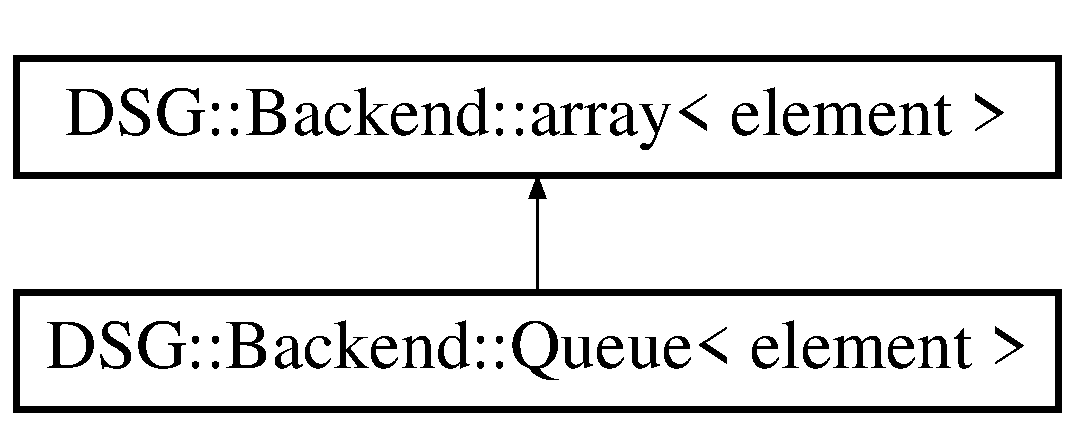
\includegraphics[height=2.000000cm]{classDSG_1_1Backend_1_1array}
\end{center}
\end{figure}
\subsection*{Public Types}
\begin{DoxyCompactItemize}
\item 
typedef element $\ast$ \hyperlink{classDSG_1_1Backend_1_1array_abfd0db2267892f4d2f397638faf85ca3}{pointer}
\item 
typedef element \& \hyperlink{classDSG_1_1Backend_1_1array_a8af2a20d445daee75e9e6b122498e0a6}{reference}
\end{DoxyCompactItemize}
\subsection*{Public Member Functions}
\begin{DoxyCompactItemize}
\item 
\hyperlink{classDSG_1_1Backend_1_1array_aa6b9a819e5a82e634956bc7ae3f4f4b2}{array} ()
\item 
\hyperlink{classDSG_1_1Backend_1_1array_aedacabe25ffa6dd6a08cd023a113eb8f}{array} (unsigned long size)
\item 
\hyperlink{classDSG_1_1Backend_1_1array_a07a41d17ec383a4b677b77213873bb6b}{array} (\hyperlink{classDSG_1_1Backend_1_1array}{array}$<$ element $>$ const \&other)
\item 
\hyperlink{classDSG_1_1Backend_1_1array}{array}$<$ element $>$ \& \hyperlink{classDSG_1_1Backend_1_1array_a84b5eb78bf672b58cc6c941d0c0705dd}{operator=} (\hyperlink{classDSG_1_1Backend_1_1array}{array}$<$ element $>$ const \&other)
\item 
virtual \hyperlink{classDSG_1_1Backend_1_1array_ad90859dd72ad8968153211d8c89b24bd}{$\sim$array} ()
\item 
element \& \hyperlink{classDSG_1_1Backend_1_1array_a69fb5ed051dd548a544f4d9ebd94fda7}{operator\mbox{[}$\,$\mbox{]}} (unsigned long const \&index)
\item 
unsigned long const \& \hyperlink{classDSG_1_1Backend_1_1array_ad31900d7cd043f7f058f7d86a36d1748}{Size} () const 
\end{DoxyCompactItemize}
\subsection*{Protected Attributes}
\begin{DoxyCompactItemize}
\item 
element $\ast$ \hyperlink{classDSG_1_1Backend_1_1array_a520f838f921d4f48852694e79da0564c}{\+\_\+array}
\item 
unsigned long \hyperlink{classDSG_1_1Backend_1_1array_a44349f32c09ebb31d5eadbe9a222cba2}{\+\_\+size}
\end{DoxyCompactItemize}


\subsection{Detailed Description}
\subsubsection*{template$<$class element$>$class D\+S\+G\+::\+Backend\+::array$<$ element $>$}



Definition at line 27 of file Queue.\+h.



\subsection{Member Typedef Documentation}
\hypertarget{classDSG_1_1Backend_1_1array_abfd0db2267892f4d2f397638faf85ca3}{\index{D\+S\+G\+::\+Backend\+::array@{D\+S\+G\+::\+Backend\+::array}!pointer@{pointer}}
\index{pointer@{pointer}!D\+S\+G\+::\+Backend\+::array@{D\+S\+G\+::\+Backend\+::array}}
\subsubsection[{pointer}]{\setlength{\rightskip}{0pt plus 5cm}template$<$class element$>$ typedef element$\ast$ {\bf D\+S\+G\+::\+Backend\+::array}$<$ element $>$\+::{\bf pointer}}}\label{classDSG_1_1Backend_1_1array_abfd0db2267892f4d2f397638faf85ca3}


Definition at line 29 of file Queue.\+h.

\hypertarget{classDSG_1_1Backend_1_1array_a8af2a20d445daee75e9e6b122498e0a6}{\index{D\+S\+G\+::\+Backend\+::array@{D\+S\+G\+::\+Backend\+::array}!reference@{reference}}
\index{reference@{reference}!D\+S\+G\+::\+Backend\+::array@{D\+S\+G\+::\+Backend\+::array}}
\subsubsection[{reference}]{\setlength{\rightskip}{0pt plus 5cm}template$<$class element$>$ typedef element\& {\bf D\+S\+G\+::\+Backend\+::array}$<$ element $>$\+::{\bf reference}}}\label{classDSG_1_1Backend_1_1array_a8af2a20d445daee75e9e6b122498e0a6}


Definition at line 30 of file Queue.\+h.



\subsection{Constructor \& Destructor Documentation}
\hypertarget{classDSG_1_1Backend_1_1array_aa6b9a819e5a82e634956bc7ae3f4f4b2}{\index{D\+S\+G\+::\+Backend\+::array@{D\+S\+G\+::\+Backend\+::array}!array@{array}}
\index{array@{array}!D\+S\+G\+::\+Backend\+::array@{D\+S\+G\+::\+Backend\+::array}}
\subsubsection[{array}]{\setlength{\rightskip}{0pt plus 5cm}template$<$class element$>$ {\bf D\+S\+G\+::\+Backend\+::array}$<$ element $>$\+::{\bf array} (
\begin{DoxyParamCaption}
{}
\end{DoxyParamCaption}
)\hspace{0.3cm}{\ttfamily [inline]}}}\label{classDSG_1_1Backend_1_1array_aa6b9a819e5a82e634956bc7ae3f4f4b2}


Definition at line 32 of file Queue.\+h.


\begin{DoxyCode}
32 :\hyperlink{classDSG_1_1Backend_1_1array_a44349f32c09ebb31d5eadbe9a222cba2}{\_size}(0),\hyperlink{classDSG_1_1Backend_1_1array_a520f838f921d4f48852694e79da0564c}{\_array}(\textcolor{keyword}{nullptr})\{\}
\end{DoxyCode}
\hypertarget{classDSG_1_1Backend_1_1array_aedacabe25ffa6dd6a08cd023a113eb8f}{\index{D\+S\+G\+::\+Backend\+::array@{D\+S\+G\+::\+Backend\+::array}!array@{array}}
\index{array@{array}!D\+S\+G\+::\+Backend\+::array@{D\+S\+G\+::\+Backend\+::array}}
\subsubsection[{array}]{\setlength{\rightskip}{0pt plus 5cm}template$<$class element$>$ {\bf D\+S\+G\+::\+Backend\+::array}$<$ element $>$\+::{\bf array} (
\begin{DoxyParamCaption}
\item[{unsigned long}]{size}
\end{DoxyParamCaption}
)\hspace{0.3cm}{\ttfamily [inline]}}}\label{classDSG_1_1Backend_1_1array_aedacabe25ffa6dd6a08cd023a113eb8f}


Definition at line 33 of file Queue.\+h.


\begin{DoxyCode}
33 :\hyperlink{classDSG_1_1Backend_1_1array_a44349f32c09ebb31d5eadbe9a222cba2}{\_size}(size),\hyperlink{classDSG_1_1Backend_1_1array_a520f838f921d4f48852694e79da0564c}{\_array}(\textcolor{keyword}{new} element[size])\{\}
\end{DoxyCode}
\hypertarget{classDSG_1_1Backend_1_1array_a07a41d17ec383a4b677b77213873bb6b}{\index{D\+S\+G\+::\+Backend\+::array@{D\+S\+G\+::\+Backend\+::array}!array@{array}}
\index{array@{array}!D\+S\+G\+::\+Backend\+::array@{D\+S\+G\+::\+Backend\+::array}}
\subsubsection[{array}]{\setlength{\rightskip}{0pt plus 5cm}template$<$class element$>$ {\bf D\+S\+G\+::\+Backend\+::array}$<$ element $>$\+::{\bf array} (
\begin{DoxyParamCaption}
\item[{{\bf array}$<$ element $>$ const \&}]{other}
\end{DoxyParamCaption}
)\hspace{0.3cm}{\ttfamily [inline]}}}\label{classDSG_1_1Backend_1_1array_a07a41d17ec383a4b677b77213873bb6b}


Definition at line 34 of file Queue.\+h.


\begin{DoxyCode}
34                                               \{
35                 \hyperlink{classDSG_1_1Backend_1_1array_a520f838f921d4f48852694e79da0564c}{\_array} = \textcolor{keyword}{new} element[other.Size()];
36                 \hyperlink{classDSG_1_1Backend_1_1array_a44349f32c09ebb31d5eadbe9a222cba2}{\_size} = other.Size();
37                 *\textcolor{keyword}{this} = other;
38             \}
\end{DoxyCode}
\hypertarget{classDSG_1_1Backend_1_1array_ad90859dd72ad8968153211d8c89b24bd}{\index{D\+S\+G\+::\+Backend\+::array@{D\+S\+G\+::\+Backend\+::array}!````~array@{$\sim$array}}
\index{````~array@{$\sim$array}!D\+S\+G\+::\+Backend\+::array@{D\+S\+G\+::\+Backend\+::array}}
\subsubsection[{$\sim$array}]{\setlength{\rightskip}{0pt plus 5cm}template$<$class element$>$ virtual {\bf D\+S\+G\+::\+Backend\+::array}$<$ element $>$\+::$\sim${\bf array} (
\begin{DoxyParamCaption}
{}
\end{DoxyParamCaption}
)\hspace{0.3cm}{\ttfamily [inline]}, {\ttfamily [virtual]}}}\label{classDSG_1_1Backend_1_1array_ad90859dd72ad8968153211d8c89b24bd}


Definition at line 52 of file Queue.\+h.


\begin{DoxyCode}
52                             \{
53                 \textcolor{keywordflow}{if} (\hyperlink{classDSG_1_1Backend_1_1array_a520f838f921d4f48852694e79da0564c}{\_array}!=\textcolor{keyword}{nullptr}) \{
54                     \textcolor{keyword}{delete} [] \hyperlink{classDSG_1_1Backend_1_1array_a520f838f921d4f48852694e79da0564c}{\_array};
55                 \}
56                 \hyperlink{classDSG_1_1Backend_1_1array_a44349f32c09ebb31d5eadbe9a222cba2}{\_size}=0;
57             \}
\end{DoxyCode}


\subsection{Member Function Documentation}
\hypertarget{classDSG_1_1Backend_1_1array_a84b5eb78bf672b58cc6c941d0c0705dd}{\index{D\+S\+G\+::\+Backend\+::array@{D\+S\+G\+::\+Backend\+::array}!operator=@{operator=}}
\index{operator=@{operator=}!D\+S\+G\+::\+Backend\+::array@{D\+S\+G\+::\+Backend\+::array}}
\subsubsection[{operator=}]{\setlength{\rightskip}{0pt plus 5cm}template$<$class element$>$ {\bf array}$<$element$>$\& {\bf D\+S\+G\+::\+Backend\+::array}$<$ element $>$\+::operator= (
\begin{DoxyParamCaption}
\item[{{\bf array}$<$ element $>$ const \&}]{other}
\end{DoxyParamCaption}
)\hspace{0.3cm}{\ttfamily [inline]}}}\label{classDSG_1_1Backend_1_1array_a84b5eb78bf672b58cc6c941d0c0705dd}


Definition at line 39 of file Queue.\+h.


\begin{DoxyCode}
39                                                                   \{
40                 \textcolor{keywordflow}{if} (\hyperlink{classDSG_1_1Backend_1_1array_a44349f32c09ebb31d5eadbe9a222cba2}{\_size}!=other.\_size) \{
41                     \textcolor{keywordflow}{if} (\hyperlink{classDSG_1_1Backend_1_1array_a520f838f921d4f48852694e79da0564c}{\_array}!=\textcolor{keyword}{nullptr}) \{
42                         \textcolor{keyword}{delete} [] \hyperlink{classDSG_1_1Backend_1_1array_a520f838f921d4f48852694e79da0564c}{\_array};
43                     \}
44                     \hyperlink{classDSG_1_1Backend_1_1array_a44349f32c09ebb31d5eadbe9a222cba2}{\_size} = other.\_size;
45                     \hyperlink{classDSG_1_1Backend_1_1array_a520f838f921d4f48852694e79da0564c}{\_array} = \textcolor{keyword}{new} element[\hyperlink{classDSG_1_1Backend_1_1array_a44349f32c09ebb31d5eadbe9a222cba2}{\_size}];
46                 \}
47                 \textcolor{keywordflow}{for} (\textcolor{keywordtype}{int} i=0; i<\hyperlink{classDSG_1_1Backend_1_1array_a44349f32c09ebb31d5eadbe9a222cba2}{\_size}; ++i) \{
48                     \hyperlink{classDSG_1_1Backend_1_1array_a520f838f921d4f48852694e79da0564c}{\_array}[i] = other.\_array[i];
49                 \}
50                 \textcolor{keywordflow}{return} *\textcolor{keyword}{this};
51             \}
\end{DoxyCode}
\hypertarget{classDSG_1_1Backend_1_1array_a69fb5ed051dd548a544f4d9ebd94fda7}{\index{D\+S\+G\+::\+Backend\+::array@{D\+S\+G\+::\+Backend\+::array}!operator\mbox{[}$\,$\mbox{]}@{operator[]}}
\index{operator\mbox{[}$\,$\mbox{]}@{operator[]}!D\+S\+G\+::\+Backend\+::array@{D\+S\+G\+::\+Backend\+::array}}
\subsubsection[{operator[]}]{\setlength{\rightskip}{0pt plus 5cm}template$<$class element$>$ element\& {\bf D\+S\+G\+::\+Backend\+::array}$<$ element $>$\+::operator\mbox{[}$\,$\mbox{]} (
\begin{DoxyParamCaption}
\item[{unsigned long const \&}]{index}
\end{DoxyParamCaption}
)\hspace{0.3cm}{\ttfamily [inline]}}}\label{classDSG_1_1Backend_1_1array_a69fb5ed051dd548a544f4d9ebd94fda7}


Definition at line 58 of file Queue.\+h.


\begin{DoxyCode}
58                                                            \{
59 \textcolor{preprocessor}{#ifdef DEBUG}
60                 assert(index<\hyperlink{classDSG_1_1Backend_1_1array_a44349f32c09ebb31d5eadbe9a222cba2}{\_size});
61 \textcolor{preprocessor}{#endif}
62                 \textcolor{keywordflow}{return} \hyperlink{classDSG_1_1Backend_1_1array_a520f838f921d4f48852694e79da0564c}{\_array}[index];
63             \}
\end{DoxyCode}
\hypertarget{classDSG_1_1Backend_1_1array_ad31900d7cd043f7f058f7d86a36d1748}{\index{D\+S\+G\+::\+Backend\+::array@{D\+S\+G\+::\+Backend\+::array}!Size@{Size}}
\index{Size@{Size}!D\+S\+G\+::\+Backend\+::array@{D\+S\+G\+::\+Backend\+::array}}
\subsubsection[{Size}]{\setlength{\rightskip}{0pt plus 5cm}template$<$class element$>$ unsigned long const\& {\bf D\+S\+G\+::\+Backend\+::array}$<$ element $>$\+::Size (
\begin{DoxyParamCaption}
{}
\end{DoxyParamCaption}
) const\hspace{0.3cm}{\ttfamily [inline]}}}\label{classDSG_1_1Backend_1_1array_ad31900d7cd043f7f058f7d86a36d1748}


Definition at line 64 of file Queue.\+h.


\begin{DoxyCode}
64                                             \{
65                 \textcolor{keywordflow}{return} \hyperlink{classDSG_1_1Backend_1_1array_a44349f32c09ebb31d5eadbe9a222cba2}{\_size};
66             \}
\end{DoxyCode}


\subsection{Member Data Documentation}
\hypertarget{classDSG_1_1Backend_1_1array_a520f838f921d4f48852694e79da0564c}{\index{D\+S\+G\+::\+Backend\+::array@{D\+S\+G\+::\+Backend\+::array}!\+\_\+array@{\+\_\+array}}
\index{\+\_\+array@{\+\_\+array}!D\+S\+G\+::\+Backend\+::array@{D\+S\+G\+::\+Backend\+::array}}
\subsubsection[{\+\_\+array}]{\setlength{\rightskip}{0pt plus 5cm}template$<$class element$>$ element$\ast$ {\bf D\+S\+G\+::\+Backend\+::array}$<$ element $>$\+::\+\_\+array\hspace{0.3cm}{\ttfamily [protected]}}}\label{classDSG_1_1Backend_1_1array_a520f838f921d4f48852694e79da0564c}


Definition at line 68 of file Queue.\+h.

\hypertarget{classDSG_1_1Backend_1_1array_a44349f32c09ebb31d5eadbe9a222cba2}{\index{D\+S\+G\+::\+Backend\+::array@{D\+S\+G\+::\+Backend\+::array}!\+\_\+size@{\+\_\+size}}
\index{\+\_\+size@{\+\_\+size}!D\+S\+G\+::\+Backend\+::array@{D\+S\+G\+::\+Backend\+::array}}
\subsubsection[{\+\_\+size}]{\setlength{\rightskip}{0pt plus 5cm}template$<$class element$>$ unsigned long {\bf D\+S\+G\+::\+Backend\+::array}$<$ element $>$\+::\+\_\+size\hspace{0.3cm}{\ttfamily [protected]}}}\label{classDSG_1_1Backend_1_1array_a44349f32c09ebb31d5eadbe9a222cba2}


Definition at line 69 of file Queue.\+h.



The documentation for this class was generated from the following file\+:\begin{DoxyCompactItemize}
\item 
/\+Users/alexanderzywicki/\+Documents/\+School\+\_\+\+Stuff/\+Fall\+\_\+2014/\+Digital\+\_\+\+Signal\+\_\+\+Generation\+\_\+and\+\_\+\+Analysis/src/include/\hyperlink{Queue_8h}{Queue.\+h}\end{DoxyCompactItemize}

\hypertarget{classDSG_1_1BLIT}{\section{D\+S\+G\+:\+:B\+L\+I\+T Class Reference}
\label{classDSG_1_1BLIT}\index{D\+S\+G\+::\+B\+L\+I\+T@{D\+S\+G\+::\+B\+L\+I\+T}}
}


See file $\sim$/\+Research/alias-\/free-\/digital-\/synthesis-\/of-\/classic-\/analog-\/waveforms.pdf for details of concept.  




{\ttfamily \#include $<$B\+L\+I\+T.\+h$>$}

Inheritance diagram for D\+S\+G\+:\+:B\+L\+I\+T\+:\begin{figure}[H]
\begin{center}
\leavevmode
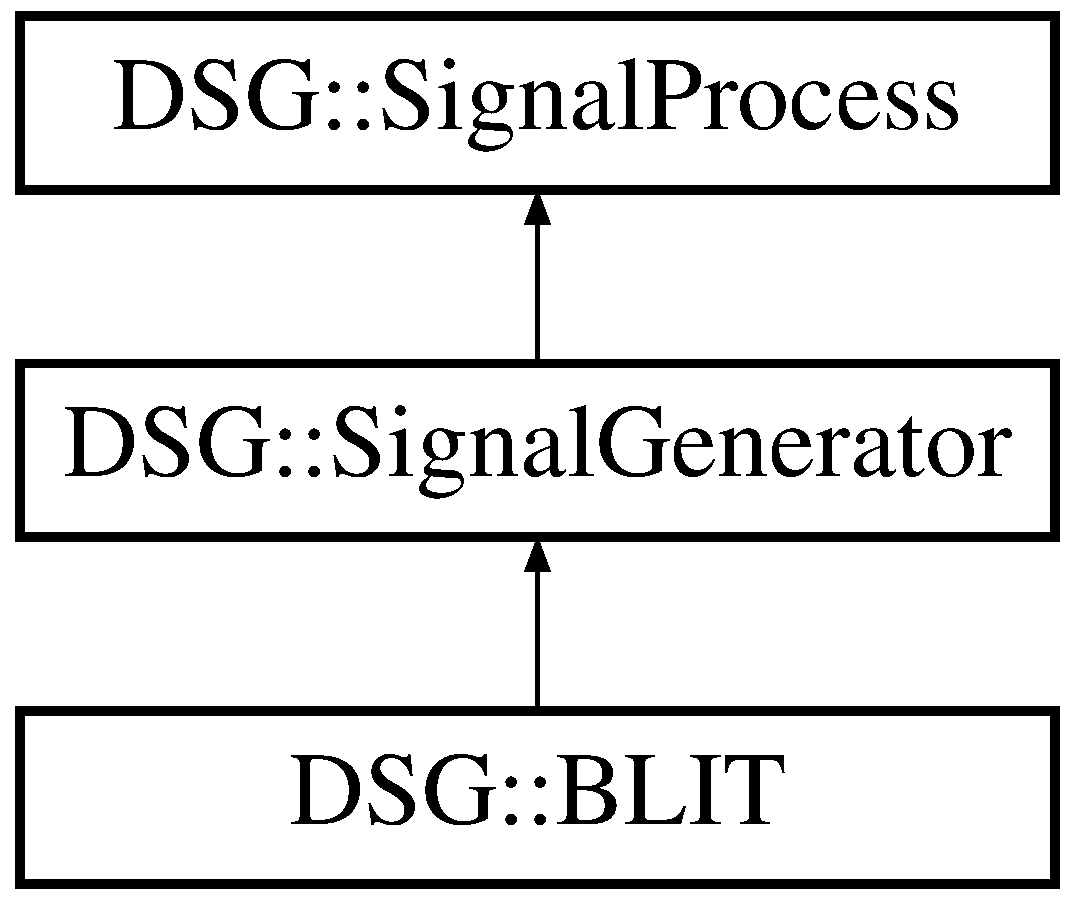
\includegraphics[height=4.000000cm]{classDSG_1_1BLIT}
\end{center}
\end{figure}
\subsection*{Public Member Functions}
\begin{DoxyCompactItemize}
\item 
\hyperlink{classDSG_1_1BLIT_adce48aa8a4f30706a339361a565b1b75}{B\+L\+I\+T} ()
\item 
\hyperlink{classDSG_1_1BLIT_a2155ccee2dc729bf6210c543190dbe35}{B\+L\+I\+T} (double const \&frequency, double const \&phase\+\_\+offset)
\item 
virtual \hyperlink{classDSG_1_1BLIT_a69b280e6c5fd20d0d294dde1c496db63}{$\sim$\+B\+L\+I\+T} ()
\item 
virtual double const \& \hyperlink{classDSG_1_1BLIT_a67b698a54f37c361945cae3e137af76f}{Frequency} (double const \&value)
\item 
virtual bool \hyperlink{classDSG_1_1BLIT_a0f769ac63ee884a6d3899b38d6c2944c}{Perform} (\hyperlink{classDSG_1_1Sample}{Sample} \&signal)
\item 
virtual bool \hyperlink{classDSG_1_1BLIT_ae464457074d366c46f42b53b59d82ecb}{Perform} (\hyperlink{classDSG_1_1RingBuffer}{Ring\+Buffer} \&signal)
\item 
virtual bool \hyperlink{classDSG_1_1SignalProcess_afdb8220100418893950c1161dd24db67}{Perform} (\hyperlink{classDSG_1_1Sample_aaf2e30d73911eccea99b53eeee15b612}{Sample\+::\+Sample} \&signal)=0
\item 
virtual double const \& \hyperlink{classDSG_1_1SignalGenerator_aedac746c5a70818d120858542ecb7c45}{Frequency} () const 
\item 
virtual double const \& \hyperlink{classDSG_1_1SignalGenerator_a1ce521847edd0b837fd840998f906b4b}{Phase\+Offset} () const 
\item 
virtual double const \& \hyperlink{classDSG_1_1SignalGenerator_a08b71b1f30ba65e629642c570291dc0e}{Phase\+Offset} (double const \&value)
\end{DoxyCompactItemize}
\subsection*{Protected Member Functions}
\begin{DoxyCompactItemize}
\item 
virtual void \hyperlink{classDSG_1_1BLIT_ac59980dee201683229d5a106f941298b}{update\+Harms} ()
\item 
double \hyperlink{classDSG_1_1SignalGenerator_ac0d781b8673b3a283bf7c133290ede50}{\+\_\+pstep} ()
\item 
double \hyperlink{classDSG_1_1SignalGenerator_ae660eb4caa88b8d278f8d24d0908a487}{\+\_\+pstep\+\_\+rad} ()
\item 
void \hyperlink{classDSG_1_1SignalGenerator_a05baccb38d1e52860d4fcf7cb8430efc}{\+\_\+psync} ()
\end{DoxyCompactItemize}
\subsection*{Protected Attributes}
\begin{DoxyCompactItemize}
\item 
\hyperlink{classDSG_1_1Sample}{Sample} \hyperlink{classDSG_1_1BLIT_a4fa5d5d8a8d5dd64e027067d0018570d}{\+\_\+sample}
\item 
unsigned long \hyperlink{classDSG_1_1BLIT_afe749d26f1503740bedd54f5147bc66d}{\+\_\+n\+Harms}
\item 
unsigned long \hyperlink{classDSG_1_1BLIT_a93504a847d83314bbd9020750820242b}{m\+\_\+}
\item 
float \hyperlink{classDSG_1_1BLIT_a392dc88ed2691c6637a6afe8607881c6}{phs}
\item 
float \hyperlink{classDSG_1_1BLIT_ac0570d5d963ca947e8860a547df7b9dc}{tmp}
\item 
float \hyperlink{classDSG_1_1BLIT_a664b4f06a7b5657261cfaa30dd503c16}{\+\_\+denominator}
\item 
double \hyperlink{classDSG_1_1SignalGenerator_aa10f6c85d9adee901139ea7fb346f39d}{\+\_\+rate}
\item 
double \hyperlink{classDSG_1_1SignalGenerator_a67e296e3506dcdf09402c667cddff9ac}{\+\_\+frequency}
\item 
double \hyperlink{classDSG_1_1SignalGenerator_ac2271b582bf699275f077ecb642a8cd9}{\+\_\+phasor}
\end{DoxyCompactItemize}


\subsection{Detailed Description}
See file $\sim$/\+Research/alias-\/free-\/digital-\/synthesis-\/of-\/classic-\/analog-\/waveforms.pdf for details of concept. 

Definition at line 21 of file B\+L\+I\+T.\+h.



\subsection{Constructor \& Destructor Documentation}
\hypertarget{classDSG_1_1BLIT_adce48aa8a4f30706a339361a565b1b75}{\index{D\+S\+G\+::\+B\+L\+I\+T@{D\+S\+G\+::\+B\+L\+I\+T}!B\+L\+I\+T@{B\+L\+I\+T}}
\index{B\+L\+I\+T@{B\+L\+I\+T}!D\+S\+G\+::\+B\+L\+I\+T@{D\+S\+G\+::\+B\+L\+I\+T}}
\subsubsection[{B\+L\+I\+T}]{\setlength{\rightskip}{0pt plus 5cm}D\+S\+G\+::\+B\+L\+I\+T\+::\+B\+L\+I\+T (
\begin{DoxyParamCaption}
{}
\end{DoxyParamCaption}
)}}\label{classDSG_1_1BLIT_adce48aa8a4f30706a339361a565b1b75}


Definition at line 11 of file B\+L\+I\+T.\+cpp.


\begin{DoxyCode}
11              :\hyperlink{classDSG_1_1SignalGenerator_a13ebda67fcdc880ef41aff501cc23fc3}{SignalGenerator}(),\hyperlink{classDSG_1_1BLIT_a392dc88ed2691c6637a6afe8607881c6}{phs}(0)\{
12     \hyperlink{classDSG_1_1BLIT_ac59980dee201683229d5a106f941298b}{updateHarms}();
13 \}
\end{DoxyCode}
\hypertarget{classDSG_1_1BLIT_a2155ccee2dc729bf6210c543190dbe35}{\index{D\+S\+G\+::\+B\+L\+I\+T@{D\+S\+G\+::\+B\+L\+I\+T}!B\+L\+I\+T@{B\+L\+I\+T}}
\index{B\+L\+I\+T@{B\+L\+I\+T}!D\+S\+G\+::\+B\+L\+I\+T@{D\+S\+G\+::\+B\+L\+I\+T}}
\subsubsection[{B\+L\+I\+T}]{\setlength{\rightskip}{0pt plus 5cm}D\+S\+G\+::\+B\+L\+I\+T\+::\+B\+L\+I\+T (
\begin{DoxyParamCaption}
\item[{double const \&}]{frequency, }
\item[{double const \&}]{phase\+\_\+offset}
\end{DoxyParamCaption}
)}}\label{classDSG_1_1BLIT_a2155ccee2dc729bf6210c543190dbe35}


Definition at line 14 of file B\+L\+I\+T.\+cpp.


\begin{DoxyCode}
14                                                                :\hyperlink{classDSG_1_1SignalGenerator_a13ebda67fcdc880ef41aff501cc23fc3}{SignalGenerator}(frequency,
      phase\_offset)\{
15     \hyperlink{classDSG_1_1BLIT_afe749d26f1503740bedd54f5147bc66d}{\_nHarms} = ( \hyperlink{namespaceDSG_a0c5c3a251b3688398da18138c5efe4bf}{Sample\_Rate}()*0.5)/\hyperlink{classDSG_1_1SignalGenerator_a67e296e3506dcdf09402c667cddff9ac}{\_frequency};
16     \hyperlink{classDSG_1_1BLIT_ac59980dee201683229d5a106f941298b}{updateHarms}();
17 \}
\end{DoxyCode}
\hypertarget{classDSG_1_1BLIT_a69b280e6c5fd20d0d294dde1c496db63}{\index{D\+S\+G\+::\+B\+L\+I\+T@{D\+S\+G\+::\+B\+L\+I\+T}!````~B\+L\+I\+T@{$\sim$\+B\+L\+I\+T}}
\index{````~B\+L\+I\+T@{$\sim$\+B\+L\+I\+T}!D\+S\+G\+::\+B\+L\+I\+T@{D\+S\+G\+::\+B\+L\+I\+T}}
\subsubsection[{$\sim$\+B\+L\+I\+T}]{\setlength{\rightskip}{0pt plus 5cm}D\+S\+G\+::\+B\+L\+I\+T\+::$\sim$\+B\+L\+I\+T (
\begin{DoxyParamCaption}
{}
\end{DoxyParamCaption}
)\hspace{0.3cm}{\ttfamily [virtual]}}}\label{classDSG_1_1BLIT_a69b280e6c5fd20d0d294dde1c496db63}


Definition at line 18 of file B\+L\+I\+T.\+cpp.


\begin{DoxyCode}
18 \{\}
\end{DoxyCode}


\subsection{Member Function Documentation}
\hypertarget{classDSG_1_1SignalGenerator_ac0d781b8673b3a283bf7c133290ede50}{\index{D\+S\+G\+::\+B\+L\+I\+T@{D\+S\+G\+::\+B\+L\+I\+T}!\+\_\+pstep@{\+\_\+pstep}}
\index{\+\_\+pstep@{\+\_\+pstep}!D\+S\+G\+::\+B\+L\+I\+T@{D\+S\+G\+::\+B\+L\+I\+T}}
\subsubsection[{\+\_\+pstep}]{\setlength{\rightskip}{0pt plus 5cm}double D\+S\+G\+::\+Signal\+Generator\+::\+\_\+pstep (
\begin{DoxyParamCaption}
{}
\end{DoxyParamCaption}
)\hspace{0.3cm}{\ttfamily [inline]}, {\ttfamily [protected]}, {\ttfamily [inherited]}}}\label{classDSG_1_1SignalGenerator_ac0d781b8673b3a283bf7c133290ede50}


Definition at line 52 of file Signal\+Generator.\+h.


\begin{DoxyCode}
52                                          \{
53         value = \hyperlink{classDSG_1_1SignalGenerator_ac2271b582bf699275f077ecb642a8cd9}{\_phasor};
54         \hyperlink{classDSG_1_1SignalGenerator_ac2271b582bf699275f077ecb642a8cd9}{\_phasor}+=\hyperlink{classDSG_1_1SignalGenerator_aa10f6c85d9adee901139ea7fb346f39d}{\_rate};
55         \hyperlink{classDSG_1_1SignalGenerator_ac2271b582bf699275f077ecb642a8cd9}{\_phasor}>1?\hyperlink{classDSG_1_1SignalGenerator_ac2271b582bf699275f077ecb642a8cd9}{\_phasor}-=1:0;\textcolor{comment}{//cheaper cheaper %1}
56         \textcolor{comment}{//\_phasor -= (unsigned long)\_phasor;//cheaper %1}
57         \textcolor{keywordflow}{return} value;
58     \}
\end{DoxyCode}
\hypertarget{classDSG_1_1SignalGenerator_ae660eb4caa88b8d278f8d24d0908a487}{\index{D\+S\+G\+::\+B\+L\+I\+T@{D\+S\+G\+::\+B\+L\+I\+T}!\+\_\+pstep\+\_\+rad@{\+\_\+pstep\+\_\+rad}}
\index{\+\_\+pstep\+\_\+rad@{\+\_\+pstep\+\_\+rad}!D\+S\+G\+::\+B\+L\+I\+T@{D\+S\+G\+::\+B\+L\+I\+T}}
\subsubsection[{\+\_\+pstep\+\_\+rad}]{\setlength{\rightskip}{0pt plus 5cm}double D\+S\+G\+::\+Signal\+Generator\+::\+\_\+pstep\+\_\+rad (
\begin{DoxyParamCaption}
{}
\end{DoxyParamCaption}
)\hspace{0.3cm}{\ttfamily [inline]}, {\ttfamily [protected]}, {\ttfamily [inherited]}}}\label{classDSG_1_1SignalGenerator_ae660eb4caa88b8d278f8d24d0908a487}


Definition at line 59 of file Signal\+Generator.\+h.


\begin{DoxyCode}
59                                              \{
60         \textcolor{keywordflow}{return} \hyperlink{PI_8h_a4912c64aec0c943b7985db6cb61ff83a}{TWOPI} * \hyperlink{classDSG_1_1SignalGenerator_ac0d781b8673b3a283bf7c133290ede50}{\_pstep}();
61     \}
\end{DoxyCode}
\hypertarget{classDSG_1_1SignalGenerator_a05baccb38d1e52860d4fcf7cb8430efc}{\index{D\+S\+G\+::\+B\+L\+I\+T@{D\+S\+G\+::\+B\+L\+I\+T}!\+\_\+psync@{\+\_\+psync}}
\index{\+\_\+psync@{\+\_\+psync}!D\+S\+G\+::\+B\+L\+I\+T@{D\+S\+G\+::\+B\+L\+I\+T}}
\subsubsection[{\+\_\+psync}]{\setlength{\rightskip}{0pt plus 5cm}void D\+S\+G\+::\+Signal\+Generator\+::\+\_\+psync (
\begin{DoxyParamCaption}
{}
\end{DoxyParamCaption}
)\hspace{0.3cm}{\ttfamily [inline]}, {\ttfamily [protected]}, {\ttfamily [inherited]}}}\label{classDSG_1_1SignalGenerator_a05baccb38d1e52860d4fcf7cb8430efc}


Definition at line 62 of file Signal\+Generator.\+h.


\begin{DoxyCode}
62                                        \{
63         \hyperlink{classDSG_1_1SignalGenerator_ac2271b582bf699275f077ecb642a8cd9}{\_phasor} = \_phase\_offset;
64     \}
\end{DoxyCode}
\hypertarget{classDSG_1_1SignalGenerator_aedac746c5a70818d120858542ecb7c45}{\index{D\+S\+G\+::\+B\+L\+I\+T@{D\+S\+G\+::\+B\+L\+I\+T}!Frequency@{Frequency}}
\index{Frequency@{Frequency}!D\+S\+G\+::\+B\+L\+I\+T@{D\+S\+G\+::\+B\+L\+I\+T}}
\subsubsection[{Frequency}]{\setlength{\rightskip}{0pt plus 5cm}double const \& D\+S\+G\+::\+Signal\+Generator\+::\+Frequency (
\begin{DoxyParamCaption}
{}
\end{DoxyParamCaption}
) const\hspace{0.3cm}{\ttfamily [virtual]}, {\ttfamily [inherited]}}}\label{classDSG_1_1SignalGenerator_aedac746c5a70818d120858542ecb7c45}


Definition at line 14 of file Signal\+Generator.\+cpp.


\begin{DoxyCode}
14                                                 \{
15     \textcolor{keywordflow}{return} \hyperlink{classDSG_1_1SignalGenerator_a67e296e3506dcdf09402c667cddff9ac}{\_frequency};
16 \}
\end{DoxyCode}
\hypertarget{classDSG_1_1BLIT_a67b698a54f37c361945cae3e137af76f}{\index{D\+S\+G\+::\+B\+L\+I\+T@{D\+S\+G\+::\+B\+L\+I\+T}!Frequency@{Frequency}}
\index{Frequency@{Frequency}!D\+S\+G\+::\+B\+L\+I\+T@{D\+S\+G\+::\+B\+L\+I\+T}}
\subsubsection[{Frequency}]{\setlength{\rightskip}{0pt plus 5cm}double const \& D\+S\+G\+::\+B\+L\+I\+T\+::\+Frequency (
\begin{DoxyParamCaption}
\item[{double const \&}]{value}
\end{DoxyParamCaption}
)\hspace{0.3cm}{\ttfamily [virtual]}}}\label{classDSG_1_1BLIT_a67b698a54f37c361945cae3e137af76f}


Reimplemented from \hyperlink{classDSG_1_1SignalGenerator_ae3ce8d45bafabbd86a0f535b15c3cd46}{D\+S\+G\+::\+Signal\+Generator}.



Definition at line 20 of file B\+L\+I\+T.\+cpp.


\begin{DoxyCode}
20                                                    \{
21     this->\hyperlink{classDSG_1_1SignalGenerator_aedac746c5a70818d120858542ecb7c45}{SignalGenerator::Frequency}(value);
22     \hyperlink{classDSG_1_1BLIT_afe749d26f1503740bedd54f5147bc66d}{\_nHarms} = ( \hyperlink{namespaceDSG_a0c5c3a251b3688398da18138c5efe4bf}{Sample\_Rate}()*0.5)/\hyperlink{classDSG_1_1SignalGenerator_a67e296e3506dcdf09402c667cddff9ac}{\_frequency};
23     \hyperlink{classDSG_1_1BLIT_ac59980dee201683229d5a106f941298b}{updateHarms}();
24     \textcolor{keywordflow}{return} this->\hyperlink{classDSG_1_1SignalGenerator_a67e296e3506dcdf09402c667cddff9ac}{\_frequency};
25 \}
\end{DoxyCode}
\hypertarget{classDSG_1_1SignalProcess_afdb8220100418893950c1161dd24db67}{\index{D\+S\+G\+::\+B\+L\+I\+T@{D\+S\+G\+::\+B\+L\+I\+T}!Perform@{Perform}}
\index{Perform@{Perform}!D\+S\+G\+::\+B\+L\+I\+T@{D\+S\+G\+::\+B\+L\+I\+T}}
\subsubsection[{Perform}]{\setlength{\rightskip}{0pt plus 5cm}virtual bool D\+S\+G\+::\+Signal\+Process\+::\+Perform (
\begin{DoxyParamCaption}
\item[{{\bf Sample\+::\+Sample} \&}]{signal}
\end{DoxyParamCaption}
)\hspace{0.3cm}{\ttfamily [inline]}, {\ttfamily [pure virtual]}, {\ttfamily [inherited]}}}\label{classDSG_1_1SignalProcess_afdb8220100418893950c1161dd24db67}
\hypertarget{classDSG_1_1BLIT_a0f769ac63ee884a6d3899b38d6c2944c}{\index{D\+S\+G\+::\+B\+L\+I\+T@{D\+S\+G\+::\+B\+L\+I\+T}!Perform@{Perform}}
\index{Perform@{Perform}!D\+S\+G\+::\+B\+L\+I\+T@{D\+S\+G\+::\+B\+L\+I\+T}}
\subsubsection[{Perform}]{\setlength{\rightskip}{0pt plus 5cm}bool D\+S\+G\+::\+B\+L\+I\+T\+::\+Perform (
\begin{DoxyParamCaption}
\item[{{\bf Sample} \&}]{signal}
\end{DoxyParamCaption}
)\hspace{0.3cm}{\ttfamily [inline]}, {\ttfamily [virtual]}}}\label{classDSG_1_1BLIT_a0f769ac63ee884a6d3899b38d6c2944c}


Reimplemented from \hyperlink{classDSG_1_1SignalGenerator_a95d485b68d874938ac93644b121607b9}{D\+S\+G\+::\+Signal\+Generator}.



Definition at line 39 of file B\+L\+I\+T.\+h.


\begin{DoxyCode}
39                                             \{
40 \textcolor{preprocessor}{#warning Untested BLIT Perform}
41         \hyperlink{classDSG_1_1BLIT_a392dc88ed2691c6637a6afe8607881c6}{phs} =\hyperlink{classDSG_1_1SignalGenerator_ac0d781b8673b3a283bf7c133290ede50}{\_pstep}();
42         \hyperlink{classDSG_1_1BLIT_a664b4f06a7b5657261cfaa30dd503c16}{\_denominator} = sin(\hyperlink{classDSG_1_1BLIT_a392dc88ed2691c6637a6afe8607881c6}{phs}*\hyperlink{PI_8h_a4912c64aec0c943b7985db6cb61ff83a}{TWOPI});
43         \textcolor{keywordflow}{if} (\hyperlink{classDSG_1_1BLIT_a664b4f06a7b5657261cfaa30dd503c16}{\_denominator}<=std::numeric\_limits<float>::epsilon()) \{
44             \hyperlink{classDSG_1_1BLIT_ac0570d5d963ca947e8860a547df7b9dc}{tmp}=1.0;
45         \}\textcolor{keywordflow}{else}\{
46             \hyperlink{classDSG_1_1BLIT_ac0570d5d963ca947e8860a547df7b9dc}{tmp} = sin(\hyperlink{classDSG_1_1BLIT_a392dc88ed2691c6637a6afe8607881c6}{phs}*\hyperlink{classDSG_1_1BLIT_a93504a847d83314bbd9020750820242b}{m\_}*\hyperlink{PI_8h_a4912c64aec0c943b7985db6cb61ff83a}{TWOPI});
47             \hyperlink{classDSG_1_1BLIT_ac0570d5d963ca947e8860a547df7b9dc}{tmp}/= \hyperlink{classDSG_1_1BLIT_a93504a847d83314bbd9020750820242b}{m\_} * \hyperlink{classDSG_1_1BLIT_a664b4f06a7b5657261cfaa30dd503c16}{\_denominator};
48         \}
49         signal = \hyperlink{classDSG_1_1BLIT_ac0570d5d963ca947e8860a547df7b9dc}{tmp};
50         \textcolor{keywordflow}{return} \textcolor{keyword}{true};
51     \}
\end{DoxyCode}
\hypertarget{classDSG_1_1BLIT_ae464457074d366c46f42b53b59d82ecb}{\index{D\+S\+G\+::\+B\+L\+I\+T@{D\+S\+G\+::\+B\+L\+I\+T}!Perform@{Perform}}
\index{Perform@{Perform}!D\+S\+G\+::\+B\+L\+I\+T@{D\+S\+G\+::\+B\+L\+I\+T}}
\subsubsection[{Perform}]{\setlength{\rightskip}{0pt plus 5cm}bool D\+S\+G\+::\+B\+L\+I\+T\+::\+Perform (
\begin{DoxyParamCaption}
\item[{{\bf Ring\+Buffer} \&}]{signal}
\end{DoxyParamCaption}
)\hspace{0.3cm}{\ttfamily [inline]}, {\ttfamily [virtual]}}}\label{classDSG_1_1BLIT_ae464457074d366c46f42b53b59d82ecb}


Reimplemented from \hyperlink{classDSG_1_1SignalGenerator_abaa9aecd00b792d46166b91524b42db6}{D\+S\+G\+::\+Signal\+Generator}.



Definition at line 52 of file B\+L\+I\+T.\+h.


\begin{DoxyCode}
52                                                 \{
53         signal.Flush();
54         \textcolor{keywordflow}{while} (!signal.Full()) \{
55             \textcolor{keywordflow}{if} (\hyperlink{classDSG_1_1BLIT_a0f769ac63ee884a6d3899b38d6c2944c}{Perform}(\hyperlink{classDSG_1_1BLIT_a4fa5d5d8a8d5dd64e027067d0018570d}{\_sample})) \{
56                 \textcolor{keywordflow}{if}(signal.Write(\hyperlink{classDSG_1_1BLIT_a4fa5d5d8a8d5dd64e027067d0018570d}{\_sample}))\{
57                 \}\textcolor{keywordflow}{else} \textcolor{keywordflow}{return} \textcolor{keyword}{false};
58             \}\textcolor{keywordflow}{else} \textcolor{keywordflow}{return} \textcolor{keyword}{false};
59         \}\textcolor{keywordflow}{return} \textcolor{keyword}{true};
60     \}
\end{DoxyCode}
\hypertarget{classDSG_1_1SignalGenerator_a1ce521847edd0b837fd840998f906b4b}{\index{D\+S\+G\+::\+B\+L\+I\+T@{D\+S\+G\+::\+B\+L\+I\+T}!Phase\+Offset@{Phase\+Offset}}
\index{Phase\+Offset@{Phase\+Offset}!D\+S\+G\+::\+B\+L\+I\+T@{D\+S\+G\+::\+B\+L\+I\+T}}
\subsubsection[{Phase\+Offset}]{\setlength{\rightskip}{0pt plus 5cm}double const \& D\+S\+G\+::\+Signal\+Generator\+::\+Phase\+Offset (
\begin{DoxyParamCaption}
{}
\end{DoxyParamCaption}
) const\hspace{0.3cm}{\ttfamily [virtual]}, {\ttfamily [inherited]}}}\label{classDSG_1_1SignalGenerator_a1ce521847edd0b837fd840998f906b4b}


Definition at line 22 of file Signal\+Generator.\+cpp.


\begin{DoxyCode}
22                                                   \{
23     \textcolor{keywordflow}{return} \_phase\_offset;
24 \}
\end{DoxyCode}
\hypertarget{classDSG_1_1SignalGenerator_a08b71b1f30ba65e629642c570291dc0e}{\index{D\+S\+G\+::\+B\+L\+I\+T@{D\+S\+G\+::\+B\+L\+I\+T}!Phase\+Offset@{Phase\+Offset}}
\index{Phase\+Offset@{Phase\+Offset}!D\+S\+G\+::\+B\+L\+I\+T@{D\+S\+G\+::\+B\+L\+I\+T}}
\subsubsection[{Phase\+Offset}]{\setlength{\rightskip}{0pt plus 5cm}double const \& D\+S\+G\+::\+Signal\+Generator\+::\+Phase\+Offset (
\begin{DoxyParamCaption}
\item[{double const \&}]{value}
\end{DoxyParamCaption}
)\hspace{0.3cm}{\ttfamily [virtual]}, {\ttfamily [inherited]}}}\label{classDSG_1_1SignalGenerator_a08b71b1f30ba65e629642c570291dc0e}


Definition at line 25 of file Signal\+Generator.\+cpp.


\begin{DoxyCode}
25                                                                 \{
26     \_phase\_offset-=value;
27     \hyperlink{classDSG_1_1SignalGenerator_ac2271b582bf699275f077ecb642a8cd9}{\_phasor}-=\_phase\_offset;
28     \_phase\_offset=value;
29     \textcolor{keywordflow}{return} \_phase\_offset;
30 \}\end{DoxyCode}
\hypertarget{classDSG_1_1BLIT_ac59980dee201683229d5a106f941298b}{\index{D\+S\+G\+::\+B\+L\+I\+T@{D\+S\+G\+::\+B\+L\+I\+T}!update\+Harms@{update\+Harms}}
\index{update\+Harms@{update\+Harms}!D\+S\+G\+::\+B\+L\+I\+T@{D\+S\+G\+::\+B\+L\+I\+T}}
\subsubsection[{update\+Harms}]{\setlength{\rightskip}{0pt plus 5cm}void D\+S\+G\+::\+B\+L\+I\+T\+::update\+Harms (
\begin{DoxyParamCaption}
{}
\end{DoxyParamCaption}
)\hspace{0.3cm}{\ttfamily [protected]}, {\ttfamily [virtual]}}}\label{classDSG_1_1BLIT_ac59980dee201683229d5a106f941298b}


Reimplemented in \hyperlink{classDSG_1_1BLITSaw_ae0f3f38ca9ae61f9a377f7ca141995b3}{D\+S\+G\+::\+B\+L\+I\+T\+Saw}.



Definition at line 26 of file B\+L\+I\+T.\+cpp.


\begin{DoxyCode}
26                          \{
27     \textcolor{keywordflow}{if} (\hyperlink{classDSG_1_1BLIT_afe749d26f1503740bedd54f5147bc66d}{\_nHarms}<=0) \{
28         \textcolor{keywordtype}{size\_t} max = (size\_t)floor(0.5 * ( \hyperlink{namespaceDSG_a0c5c3a251b3688398da18138c5efe4bf}{Sample\_Rate}()/ \hyperlink{classDSG_1_1SignalGenerator_a67e296e3506dcdf09402c667cddff9ac}{\_frequency}));
29         \hyperlink{classDSG_1_1BLIT_a93504a847d83314bbd9020750820242b}{m\_} = 2* max +1;
30     \}
31     \textcolor{keywordflow}{else}\{
32         \hyperlink{classDSG_1_1BLIT_a93504a847d83314bbd9020750820242b}{m\_} = 2* \hyperlink{classDSG_1_1BLIT_afe749d26f1503740bedd54f5147bc66d}{\_nHarms} +1;
33     \}
34 \}\end{DoxyCode}


\subsection{Member Data Documentation}
\hypertarget{classDSG_1_1BLIT_a664b4f06a7b5657261cfaa30dd503c16}{\index{D\+S\+G\+::\+B\+L\+I\+T@{D\+S\+G\+::\+B\+L\+I\+T}!\+\_\+denominator@{\+\_\+denominator}}
\index{\+\_\+denominator@{\+\_\+denominator}!D\+S\+G\+::\+B\+L\+I\+T@{D\+S\+G\+::\+B\+L\+I\+T}}
\subsubsection[{\+\_\+denominator}]{\setlength{\rightskip}{0pt plus 5cm}float D\+S\+G\+::\+B\+L\+I\+T\+::\+\_\+denominator\hspace{0.3cm}{\ttfamily [protected]}}}\label{classDSG_1_1BLIT_a664b4f06a7b5657261cfaa30dd503c16}


Definition at line 37 of file B\+L\+I\+T.\+h.

\hypertarget{classDSG_1_1SignalGenerator_a67e296e3506dcdf09402c667cddff9ac}{\index{D\+S\+G\+::\+B\+L\+I\+T@{D\+S\+G\+::\+B\+L\+I\+T}!\+\_\+frequency@{\+\_\+frequency}}
\index{\+\_\+frequency@{\+\_\+frequency}!D\+S\+G\+::\+B\+L\+I\+T@{D\+S\+G\+::\+B\+L\+I\+T}}
\subsubsection[{\+\_\+frequency}]{\setlength{\rightskip}{0pt plus 5cm}double D\+S\+G\+::\+Signal\+Generator\+::\+\_\+frequency\hspace{0.3cm}{\ttfamily [protected]}, {\ttfamily [inherited]}}}\label{classDSG_1_1SignalGenerator_a67e296e3506dcdf09402c667cddff9ac}


Definition at line 28 of file Signal\+Generator.\+h.

\hypertarget{classDSG_1_1BLIT_afe749d26f1503740bedd54f5147bc66d}{\index{D\+S\+G\+::\+B\+L\+I\+T@{D\+S\+G\+::\+B\+L\+I\+T}!\+\_\+n\+Harms@{\+\_\+n\+Harms}}
\index{\+\_\+n\+Harms@{\+\_\+n\+Harms}!D\+S\+G\+::\+B\+L\+I\+T@{D\+S\+G\+::\+B\+L\+I\+T}}
\subsubsection[{\+\_\+n\+Harms}]{\setlength{\rightskip}{0pt plus 5cm}unsigned long D\+S\+G\+::\+B\+L\+I\+T\+::\+\_\+n\+Harms\hspace{0.3cm}{\ttfamily [protected]}}}\label{classDSG_1_1BLIT_afe749d26f1503740bedd54f5147bc66d}


Definition at line 33 of file B\+L\+I\+T.\+h.

\hypertarget{classDSG_1_1SignalGenerator_ac2271b582bf699275f077ecb642a8cd9}{\index{D\+S\+G\+::\+B\+L\+I\+T@{D\+S\+G\+::\+B\+L\+I\+T}!\+\_\+phasor@{\+\_\+phasor}}
\index{\+\_\+phasor@{\+\_\+phasor}!D\+S\+G\+::\+B\+L\+I\+T@{D\+S\+G\+::\+B\+L\+I\+T}}
\subsubsection[{\+\_\+phasor}]{\setlength{\rightskip}{0pt plus 5cm}double D\+S\+G\+::\+Signal\+Generator\+::\+\_\+phasor\hspace{0.3cm}{\ttfamily [protected]}, {\ttfamily [inherited]}}}\label{classDSG_1_1SignalGenerator_ac2271b582bf699275f077ecb642a8cd9}


Definition at line 38 of file Signal\+Generator.\+h.

\hypertarget{classDSG_1_1SignalGenerator_aa10f6c85d9adee901139ea7fb346f39d}{\index{D\+S\+G\+::\+B\+L\+I\+T@{D\+S\+G\+::\+B\+L\+I\+T}!\+\_\+rate@{\+\_\+rate}}
\index{\+\_\+rate@{\+\_\+rate}!D\+S\+G\+::\+B\+L\+I\+T@{D\+S\+G\+::\+B\+L\+I\+T}}
\subsubsection[{\+\_\+rate}]{\setlength{\rightskip}{0pt plus 5cm}double D\+S\+G\+::\+Signal\+Generator\+::\+\_\+rate\hspace{0.3cm}{\ttfamily [protected]}, {\ttfamily [inherited]}}}\label{classDSG_1_1SignalGenerator_aa10f6c85d9adee901139ea7fb346f39d}


Definition at line 27 of file Signal\+Generator.\+h.

\hypertarget{classDSG_1_1BLIT_a4fa5d5d8a8d5dd64e027067d0018570d}{\index{D\+S\+G\+::\+B\+L\+I\+T@{D\+S\+G\+::\+B\+L\+I\+T}!\+\_\+sample@{\+\_\+sample}}
\index{\+\_\+sample@{\+\_\+sample}!D\+S\+G\+::\+B\+L\+I\+T@{D\+S\+G\+::\+B\+L\+I\+T}}
\subsubsection[{\+\_\+sample}]{\setlength{\rightskip}{0pt plus 5cm}{\bf Sample} D\+S\+G\+::\+B\+L\+I\+T\+::\+\_\+sample\hspace{0.3cm}{\ttfamily [protected]}}}\label{classDSG_1_1BLIT_a4fa5d5d8a8d5dd64e027067d0018570d}


Definition at line 32 of file B\+L\+I\+T.\+h.

\hypertarget{classDSG_1_1BLIT_a93504a847d83314bbd9020750820242b}{\index{D\+S\+G\+::\+B\+L\+I\+T@{D\+S\+G\+::\+B\+L\+I\+T}!m\+\_\+@{m\+\_\+}}
\index{m\+\_\+@{m\+\_\+}!D\+S\+G\+::\+B\+L\+I\+T@{D\+S\+G\+::\+B\+L\+I\+T}}
\subsubsection[{m\+\_\+}]{\setlength{\rightskip}{0pt plus 5cm}unsigned long D\+S\+G\+::\+B\+L\+I\+T\+::m\+\_\+\hspace{0.3cm}{\ttfamily [protected]}}}\label{classDSG_1_1BLIT_a93504a847d83314bbd9020750820242b}


Definition at line 34 of file B\+L\+I\+T.\+h.

\hypertarget{classDSG_1_1BLIT_a392dc88ed2691c6637a6afe8607881c6}{\index{D\+S\+G\+::\+B\+L\+I\+T@{D\+S\+G\+::\+B\+L\+I\+T}!phs@{phs}}
\index{phs@{phs}!D\+S\+G\+::\+B\+L\+I\+T@{D\+S\+G\+::\+B\+L\+I\+T}}
\subsubsection[{phs}]{\setlength{\rightskip}{0pt plus 5cm}float D\+S\+G\+::\+B\+L\+I\+T\+::phs\hspace{0.3cm}{\ttfamily [protected]}}}\label{classDSG_1_1BLIT_a392dc88ed2691c6637a6afe8607881c6}


Definition at line 35 of file B\+L\+I\+T.\+h.

\hypertarget{classDSG_1_1BLIT_ac0570d5d963ca947e8860a547df7b9dc}{\index{D\+S\+G\+::\+B\+L\+I\+T@{D\+S\+G\+::\+B\+L\+I\+T}!tmp@{tmp}}
\index{tmp@{tmp}!D\+S\+G\+::\+B\+L\+I\+T@{D\+S\+G\+::\+B\+L\+I\+T}}
\subsubsection[{tmp}]{\setlength{\rightskip}{0pt plus 5cm}float D\+S\+G\+::\+B\+L\+I\+T\+::tmp\hspace{0.3cm}{\ttfamily [protected]}}}\label{classDSG_1_1BLIT_ac0570d5d963ca947e8860a547df7b9dc}


Definition at line 36 of file B\+L\+I\+T.\+h.



The documentation for this class was generated from the following files\+:\begin{DoxyCompactItemize}
\item 
/\+Users/alexanderzywicki/\+Documents/\+School\+\_\+\+Stuff/\+Fall\+\_\+2014/\+Digital\+\_\+\+Signal\+\_\+\+Generation\+\_\+and\+\_\+\+Analysis/src/include/\hyperlink{BLIT_8h}{B\+L\+I\+T.\+h}\item 
/\+Users/alexanderzywicki/\+Documents/\+School\+\_\+\+Stuff/\+Fall\+\_\+2014/\+Digital\+\_\+\+Signal\+\_\+\+Generation\+\_\+and\+\_\+\+Analysis/src/\hyperlink{BLIT_8cpp}{B\+L\+I\+T.\+cpp}\end{DoxyCompactItemize}

\hypertarget{classDSG_1_1BLITSaw}{\section{D\+S\+G\+:\+:B\+L\+I\+T\+Saw Class Reference}
\label{classDSG_1_1BLITSaw}\index{D\+S\+G\+::\+B\+L\+I\+T\+Saw@{D\+S\+G\+::\+B\+L\+I\+T\+Saw}}
}


See file $\sim$/\+Research/alias-\/free-\/digital-\/synthesis-\/of-\/classic-\/analog-\/waveforms.pdf for details of concept.  




{\ttfamily \#include $<$B\+L\+I\+T\+Saw.\+h$>$}

Inheritance diagram for D\+S\+G\+:\+:B\+L\+I\+T\+Saw\+:\begin{figure}[H]
\begin{center}
\leavevmode
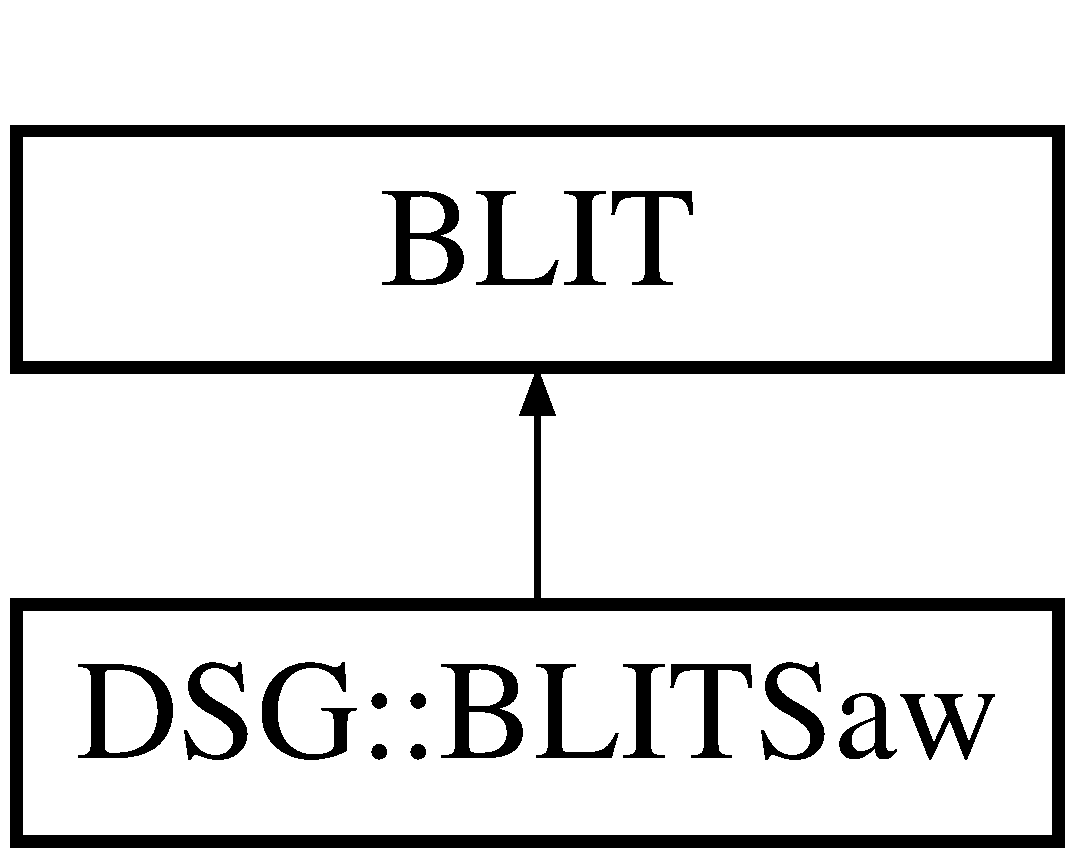
\includegraphics[height=4.000000cm]{classDSG_1_1BLITSaw}
\end{center}
\end{figure}
\subsection*{Public Member Functions}
\begin{DoxyCompactItemize}
\item 
virtual double const \& \hyperlink{classDSG_1_1SignalGenerator_aedac746c5a70818d120858542ecb7c45}{Frequency} () const 
\item 
virtual bool \hyperlink{classDSG_1_1SignalProcess_afdb8220100418893950c1161dd24db67}{Perform} (\hyperlink{classDSG_1_1Sample_aaf2e30d73911eccea99b53eeee15b612}{Sample\+::\+Sample} \&signal)=0
\item 
virtual double const \& \hyperlink{classDSG_1_1SignalGenerator_a1ce521847edd0b837fd840998f906b4b}{Phase\+Offset} () const 
\item 
virtual double const \& \hyperlink{classDSG_1_1SignalGenerator_a08b71b1f30ba65e629642c570291dc0e}{Phase\+Offset} (double const \&value)
\end{DoxyCompactItemize}
\subsection*{Protected Member Functions}
\begin{DoxyCompactItemize}
\item 
virtual void \hyperlink{classDSG_1_1BLITSaw_ae0f3f38ca9ae61f9a377f7ca141995b3}{update\+Harms} ()
\item 
double \hyperlink{classDSG_1_1SignalGenerator_ac0d781b8673b3a283bf7c133290ede50}{\+\_\+pstep} ()
\item 
double \hyperlink{classDSG_1_1SignalGenerator_ae660eb4caa88b8d278f8d24d0908a487}{\+\_\+pstep\+\_\+rad} ()
\item 
void \hyperlink{classDSG_1_1SignalGenerator_a05baccb38d1e52860d4fcf7cb8430efc}{\+\_\+psync} ()
\end{DoxyCompactItemize}
\subsection*{Protected Attributes}
\begin{DoxyCompactItemize}
\item 
float \hyperlink{classDSG_1_1BLITSaw_a71b040fae6e1d67b56c580db9f4e5c3a}{a\+\_\+}
\item 
float \hyperlink{classDSG_1_1BLITSaw_addcb3fc898bb08c71cfe81e12e2891b9}{p\+\_\+}
\item 
float \hyperlink{classDSG_1_1BLITSaw_a8ee93d1e83e22bd5ead8600ccb1f9082}{state\+\_\+}
\item 
float \hyperlink{classDSG_1_1BLITSaw_adac26390db64c9bb7e97036367bcf30f}{C2\+\_\+}
\item 
\hyperlink{classDSG_1_1Sample}{Sample} \hyperlink{classDSG_1_1BLIT_a4fa5d5d8a8d5dd64e027067d0018570d}{\+\_\+sample}
\item 
unsigned long \hyperlink{classDSG_1_1BLIT_afe749d26f1503740bedd54f5147bc66d}{\+\_\+n\+Harms}
\item 
unsigned long \hyperlink{classDSG_1_1BLIT_a93504a847d83314bbd9020750820242b}{m\+\_\+}
\item 
float \hyperlink{classDSG_1_1BLIT_a392dc88ed2691c6637a6afe8607881c6}{phs}
\item 
float \hyperlink{classDSG_1_1BLIT_ac0570d5d963ca947e8860a547df7b9dc}{tmp}
\item 
float \hyperlink{classDSG_1_1BLIT_a664b4f06a7b5657261cfaa30dd503c16}{\+\_\+denominator}
\item 
double \hyperlink{classDSG_1_1SignalGenerator_aa10f6c85d9adee901139ea7fb346f39d}{\+\_\+rate}
\item 
double \hyperlink{classDSG_1_1SignalGenerator_a67e296e3506dcdf09402c667cddff9ac}{\+\_\+frequency}
\item 
double \hyperlink{classDSG_1_1SignalGenerator_ac2271b582bf699275f077ecb642a8cd9}{\+\_\+phasor}
\end{DoxyCompactItemize}


\subsection{Detailed Description}
See file $\sim$/\+Research/alias-\/free-\/digital-\/synthesis-\/of-\/classic-\/analog-\/waveforms.pdf for details of concept. 

Definition at line 18 of file B\+L\+I\+T\+Saw.\+h.



\subsection{Member Function Documentation}
\hypertarget{classDSG_1_1SignalGenerator_ac0d781b8673b3a283bf7c133290ede50}{\index{D\+S\+G\+::\+B\+L\+I\+T\+Saw@{D\+S\+G\+::\+B\+L\+I\+T\+Saw}!\+\_\+pstep@{\+\_\+pstep}}
\index{\+\_\+pstep@{\+\_\+pstep}!D\+S\+G\+::\+B\+L\+I\+T\+Saw@{D\+S\+G\+::\+B\+L\+I\+T\+Saw}}
\subsubsection[{\+\_\+pstep}]{\setlength{\rightskip}{0pt plus 5cm}double D\+S\+G\+::\+Signal\+Generator\+::\+\_\+pstep (
\begin{DoxyParamCaption}
{}
\end{DoxyParamCaption}
)\hspace{0.3cm}{\ttfamily [inline]}, {\ttfamily [protected]}, {\ttfamily [inherited]}}}\label{classDSG_1_1SignalGenerator_ac0d781b8673b3a283bf7c133290ede50}


Definition at line 52 of file Signal\+Generator.\+h.


\begin{DoxyCode}
52                                          \{
53         value = \hyperlink{classDSG_1_1SignalGenerator_ac2271b582bf699275f077ecb642a8cd9}{\_phasor};
54         \hyperlink{classDSG_1_1SignalGenerator_ac2271b582bf699275f077ecb642a8cd9}{\_phasor}+=\hyperlink{classDSG_1_1SignalGenerator_aa10f6c85d9adee901139ea7fb346f39d}{\_rate};
55         \hyperlink{classDSG_1_1SignalGenerator_ac2271b582bf699275f077ecb642a8cd9}{\_phasor}>1?\hyperlink{classDSG_1_1SignalGenerator_ac2271b582bf699275f077ecb642a8cd9}{\_phasor}-=1:0;\textcolor{comment}{//cheaper cheaper %1}
56         \textcolor{comment}{//\_phasor -= (unsigned long)\_phasor;//cheaper %1}
57         \textcolor{keywordflow}{return} value;
58     \}
\end{DoxyCode}
\hypertarget{classDSG_1_1SignalGenerator_ae660eb4caa88b8d278f8d24d0908a487}{\index{D\+S\+G\+::\+B\+L\+I\+T\+Saw@{D\+S\+G\+::\+B\+L\+I\+T\+Saw}!\+\_\+pstep\+\_\+rad@{\+\_\+pstep\+\_\+rad}}
\index{\+\_\+pstep\+\_\+rad@{\+\_\+pstep\+\_\+rad}!D\+S\+G\+::\+B\+L\+I\+T\+Saw@{D\+S\+G\+::\+B\+L\+I\+T\+Saw}}
\subsubsection[{\+\_\+pstep\+\_\+rad}]{\setlength{\rightskip}{0pt plus 5cm}double D\+S\+G\+::\+Signal\+Generator\+::\+\_\+pstep\+\_\+rad (
\begin{DoxyParamCaption}
{}
\end{DoxyParamCaption}
)\hspace{0.3cm}{\ttfamily [inline]}, {\ttfamily [protected]}, {\ttfamily [inherited]}}}\label{classDSG_1_1SignalGenerator_ae660eb4caa88b8d278f8d24d0908a487}


Definition at line 59 of file Signal\+Generator.\+h.


\begin{DoxyCode}
59                                              \{
60         \textcolor{keywordflow}{return} \hyperlink{PI_8h_a4912c64aec0c943b7985db6cb61ff83a}{TWOPI} * \hyperlink{classDSG_1_1SignalGenerator_ac0d781b8673b3a283bf7c133290ede50}{\_pstep}();
61     \}
\end{DoxyCode}
\hypertarget{classDSG_1_1SignalGenerator_a05baccb38d1e52860d4fcf7cb8430efc}{\index{D\+S\+G\+::\+B\+L\+I\+T\+Saw@{D\+S\+G\+::\+B\+L\+I\+T\+Saw}!\+\_\+psync@{\+\_\+psync}}
\index{\+\_\+psync@{\+\_\+psync}!D\+S\+G\+::\+B\+L\+I\+T\+Saw@{D\+S\+G\+::\+B\+L\+I\+T\+Saw}}
\subsubsection[{\+\_\+psync}]{\setlength{\rightskip}{0pt plus 5cm}void D\+S\+G\+::\+Signal\+Generator\+::\+\_\+psync (
\begin{DoxyParamCaption}
{}
\end{DoxyParamCaption}
)\hspace{0.3cm}{\ttfamily [inline]}, {\ttfamily [protected]}, {\ttfamily [inherited]}}}\label{classDSG_1_1SignalGenerator_a05baccb38d1e52860d4fcf7cb8430efc}


Definition at line 62 of file Signal\+Generator.\+h.


\begin{DoxyCode}
62                                        \{
63         \hyperlink{classDSG_1_1SignalGenerator_ac2271b582bf699275f077ecb642a8cd9}{\_phasor} = \_phase\_offset;
64     \}
\end{DoxyCode}
\hypertarget{classDSG_1_1SignalGenerator_aedac746c5a70818d120858542ecb7c45}{\index{D\+S\+G\+::\+B\+L\+I\+T\+Saw@{D\+S\+G\+::\+B\+L\+I\+T\+Saw}!Frequency@{Frequency}}
\index{Frequency@{Frequency}!D\+S\+G\+::\+B\+L\+I\+T\+Saw@{D\+S\+G\+::\+B\+L\+I\+T\+Saw}}
\subsubsection[{Frequency}]{\setlength{\rightskip}{0pt plus 5cm}double const \& D\+S\+G\+::\+Signal\+Generator\+::\+Frequency (
\begin{DoxyParamCaption}
{}
\end{DoxyParamCaption}
) const\hspace{0.3cm}{\ttfamily [virtual]}, {\ttfamily [inherited]}}}\label{classDSG_1_1SignalGenerator_aedac746c5a70818d120858542ecb7c45}


Definition at line 14 of file Signal\+Generator.\+cpp.


\begin{DoxyCode}
14                                                 \{
15     \textcolor{keywordflow}{return} \hyperlink{classDSG_1_1SignalGenerator_a67e296e3506dcdf09402c667cddff9ac}{\_frequency};
16 \}
\end{DoxyCode}
\hypertarget{classDSG_1_1SignalProcess_afdb8220100418893950c1161dd24db67}{\index{D\+S\+G\+::\+B\+L\+I\+T\+Saw@{D\+S\+G\+::\+B\+L\+I\+T\+Saw}!Perform@{Perform}}
\index{Perform@{Perform}!D\+S\+G\+::\+B\+L\+I\+T\+Saw@{D\+S\+G\+::\+B\+L\+I\+T\+Saw}}
\subsubsection[{Perform}]{\setlength{\rightskip}{0pt plus 5cm}virtual bool D\+S\+G\+::\+Signal\+Process\+::\+Perform (
\begin{DoxyParamCaption}
\item[{{\bf Sample\+::\+Sample} \&}]{signal}
\end{DoxyParamCaption}
)\hspace{0.3cm}{\ttfamily [inline]}, {\ttfamily [pure virtual]}, {\ttfamily [inherited]}}}\label{classDSG_1_1SignalProcess_afdb8220100418893950c1161dd24db67}
\hypertarget{classDSG_1_1SignalGenerator_a1ce521847edd0b837fd840998f906b4b}{\index{D\+S\+G\+::\+B\+L\+I\+T\+Saw@{D\+S\+G\+::\+B\+L\+I\+T\+Saw}!Phase\+Offset@{Phase\+Offset}}
\index{Phase\+Offset@{Phase\+Offset}!D\+S\+G\+::\+B\+L\+I\+T\+Saw@{D\+S\+G\+::\+B\+L\+I\+T\+Saw}}
\subsubsection[{Phase\+Offset}]{\setlength{\rightskip}{0pt plus 5cm}double const \& D\+S\+G\+::\+Signal\+Generator\+::\+Phase\+Offset (
\begin{DoxyParamCaption}
{}
\end{DoxyParamCaption}
) const\hspace{0.3cm}{\ttfamily [virtual]}, {\ttfamily [inherited]}}}\label{classDSG_1_1SignalGenerator_a1ce521847edd0b837fd840998f906b4b}


Definition at line 22 of file Signal\+Generator.\+cpp.


\begin{DoxyCode}
22                                                   \{
23     \textcolor{keywordflow}{return} \_phase\_offset;
24 \}
\end{DoxyCode}
\hypertarget{classDSG_1_1SignalGenerator_a08b71b1f30ba65e629642c570291dc0e}{\index{D\+S\+G\+::\+B\+L\+I\+T\+Saw@{D\+S\+G\+::\+B\+L\+I\+T\+Saw}!Phase\+Offset@{Phase\+Offset}}
\index{Phase\+Offset@{Phase\+Offset}!D\+S\+G\+::\+B\+L\+I\+T\+Saw@{D\+S\+G\+::\+B\+L\+I\+T\+Saw}}
\subsubsection[{Phase\+Offset}]{\setlength{\rightskip}{0pt plus 5cm}double const \& D\+S\+G\+::\+Signal\+Generator\+::\+Phase\+Offset (
\begin{DoxyParamCaption}
\item[{double const \&}]{value}
\end{DoxyParamCaption}
)\hspace{0.3cm}{\ttfamily [virtual]}, {\ttfamily [inherited]}}}\label{classDSG_1_1SignalGenerator_a08b71b1f30ba65e629642c570291dc0e}


Definition at line 25 of file Signal\+Generator.\+cpp.


\begin{DoxyCode}
25                                                                 \{
26     \_phase\_offset-=value;
27     \hyperlink{classDSG_1_1SignalGenerator_ac2271b582bf699275f077ecb642a8cd9}{\_phasor}-=\_phase\_offset;
28     \_phase\_offset=value;
29     \textcolor{keywordflow}{return} \_phase\_offset;
30 \}\end{DoxyCode}
\hypertarget{classDSG_1_1BLITSaw_ae0f3f38ca9ae61f9a377f7ca141995b3}{\index{D\+S\+G\+::\+B\+L\+I\+T\+Saw@{D\+S\+G\+::\+B\+L\+I\+T\+Saw}!update\+Harms@{update\+Harms}}
\index{update\+Harms@{update\+Harms}!D\+S\+G\+::\+B\+L\+I\+T\+Saw@{D\+S\+G\+::\+B\+L\+I\+T\+Saw}}
\subsubsection[{update\+Harms}]{\setlength{\rightskip}{0pt plus 5cm}void D\+S\+G\+::\+B\+L\+I\+T\+Saw\+::update\+Harms (
\begin{DoxyParamCaption}
{}
\end{DoxyParamCaption}
)\hspace{0.3cm}{\ttfamily [protected]}, {\ttfamily [virtual]}}}\label{classDSG_1_1BLITSaw_ae0f3f38ca9ae61f9a377f7ca141995b3}


Reimplemented from \hyperlink{classDSG_1_1BLIT_ac59980dee201683229d5a106f941298b}{D\+S\+G\+::\+B\+L\+I\+T}.



Definition at line 23 of file B\+L\+I\+T\+Saw.\+cpp.


\begin{DoxyCode}
23                             \{
24     \textcolor{keywordflow}{if} (\hyperlink{classDSG_1_1BLIT_afe749d26f1503740bedd54f5147bc66d}{\_nHarms}<=0) \{
25         \textcolor{keywordtype}{size\_t} max = (size\_t)floor(0.5 * ( \hyperlink{namespaceDSG_a0c5c3a251b3688398da18138c5efe4bf}{Sample\_Rate}()/ \hyperlink{classDSG_1_1SignalGenerator_a67e296e3506dcdf09402c667cddff9ac}{\_frequency}));
26         \hyperlink{classDSG_1_1BLIT_a93504a847d83314bbd9020750820242b}{m\_} = 2* max +1;
27     \}
28     \textcolor{keywordflow}{else}\{
29         \hyperlink{classDSG_1_1BLIT_a93504a847d83314bbd9020750820242b}{m\_} = 2* \hyperlink{classDSG_1_1BLIT_afe749d26f1503740bedd54f5147bc66d}{\_nHarms} +1;
30     \}
31     \hyperlink{classDSG_1_1BLITSaw_a71b040fae6e1d67b56c580db9f4e5c3a}{a\_} = \hyperlink{classDSG_1_1BLIT_a93504a847d83314bbd9020750820242b}{m\_}/\hyperlink{classDSG_1_1BLITSaw_addcb3fc898bb08c71cfe81e12e2891b9}{p\_};
32 \}\end{DoxyCode}


\subsection{Member Data Documentation}
\hypertarget{classDSG_1_1BLIT_a664b4f06a7b5657261cfaa30dd503c16}{\index{D\+S\+G\+::\+B\+L\+I\+T\+Saw@{D\+S\+G\+::\+B\+L\+I\+T\+Saw}!\+\_\+denominator@{\+\_\+denominator}}
\index{\+\_\+denominator@{\+\_\+denominator}!D\+S\+G\+::\+B\+L\+I\+T\+Saw@{D\+S\+G\+::\+B\+L\+I\+T\+Saw}}
\subsubsection[{\+\_\+denominator}]{\setlength{\rightskip}{0pt plus 5cm}float D\+S\+G\+::\+B\+L\+I\+T\+::\+\_\+denominator\hspace{0.3cm}{\ttfamily [protected]}, {\ttfamily [inherited]}}}\label{classDSG_1_1BLIT_a664b4f06a7b5657261cfaa30dd503c16}


Definition at line 37 of file B\+L\+I\+T.\+h.

\hypertarget{classDSG_1_1SignalGenerator_a67e296e3506dcdf09402c667cddff9ac}{\index{D\+S\+G\+::\+B\+L\+I\+T\+Saw@{D\+S\+G\+::\+B\+L\+I\+T\+Saw}!\+\_\+frequency@{\+\_\+frequency}}
\index{\+\_\+frequency@{\+\_\+frequency}!D\+S\+G\+::\+B\+L\+I\+T\+Saw@{D\+S\+G\+::\+B\+L\+I\+T\+Saw}}
\subsubsection[{\+\_\+frequency}]{\setlength{\rightskip}{0pt plus 5cm}double D\+S\+G\+::\+Signal\+Generator\+::\+\_\+frequency\hspace{0.3cm}{\ttfamily [protected]}, {\ttfamily [inherited]}}}\label{classDSG_1_1SignalGenerator_a67e296e3506dcdf09402c667cddff9ac}


Definition at line 28 of file Signal\+Generator.\+h.

\hypertarget{classDSG_1_1BLIT_afe749d26f1503740bedd54f5147bc66d}{\index{D\+S\+G\+::\+B\+L\+I\+T\+Saw@{D\+S\+G\+::\+B\+L\+I\+T\+Saw}!\+\_\+n\+Harms@{\+\_\+n\+Harms}}
\index{\+\_\+n\+Harms@{\+\_\+n\+Harms}!D\+S\+G\+::\+B\+L\+I\+T\+Saw@{D\+S\+G\+::\+B\+L\+I\+T\+Saw}}
\subsubsection[{\+\_\+n\+Harms}]{\setlength{\rightskip}{0pt plus 5cm}unsigned long D\+S\+G\+::\+B\+L\+I\+T\+::\+\_\+n\+Harms\hspace{0.3cm}{\ttfamily [protected]}, {\ttfamily [inherited]}}}\label{classDSG_1_1BLIT_afe749d26f1503740bedd54f5147bc66d}


Definition at line 33 of file B\+L\+I\+T.\+h.

\hypertarget{classDSG_1_1SignalGenerator_ac2271b582bf699275f077ecb642a8cd9}{\index{D\+S\+G\+::\+B\+L\+I\+T\+Saw@{D\+S\+G\+::\+B\+L\+I\+T\+Saw}!\+\_\+phasor@{\+\_\+phasor}}
\index{\+\_\+phasor@{\+\_\+phasor}!D\+S\+G\+::\+B\+L\+I\+T\+Saw@{D\+S\+G\+::\+B\+L\+I\+T\+Saw}}
\subsubsection[{\+\_\+phasor}]{\setlength{\rightskip}{0pt plus 5cm}double D\+S\+G\+::\+Signal\+Generator\+::\+\_\+phasor\hspace{0.3cm}{\ttfamily [protected]}, {\ttfamily [inherited]}}}\label{classDSG_1_1SignalGenerator_ac2271b582bf699275f077ecb642a8cd9}


Definition at line 38 of file Signal\+Generator.\+h.

\hypertarget{classDSG_1_1SignalGenerator_aa10f6c85d9adee901139ea7fb346f39d}{\index{D\+S\+G\+::\+B\+L\+I\+T\+Saw@{D\+S\+G\+::\+B\+L\+I\+T\+Saw}!\+\_\+rate@{\+\_\+rate}}
\index{\+\_\+rate@{\+\_\+rate}!D\+S\+G\+::\+B\+L\+I\+T\+Saw@{D\+S\+G\+::\+B\+L\+I\+T\+Saw}}
\subsubsection[{\+\_\+rate}]{\setlength{\rightskip}{0pt plus 5cm}double D\+S\+G\+::\+Signal\+Generator\+::\+\_\+rate\hspace{0.3cm}{\ttfamily [protected]}, {\ttfamily [inherited]}}}\label{classDSG_1_1SignalGenerator_aa10f6c85d9adee901139ea7fb346f39d}


Definition at line 27 of file Signal\+Generator.\+h.

\hypertarget{classDSG_1_1BLIT_a4fa5d5d8a8d5dd64e027067d0018570d}{\index{D\+S\+G\+::\+B\+L\+I\+T\+Saw@{D\+S\+G\+::\+B\+L\+I\+T\+Saw}!\+\_\+sample@{\+\_\+sample}}
\index{\+\_\+sample@{\+\_\+sample}!D\+S\+G\+::\+B\+L\+I\+T\+Saw@{D\+S\+G\+::\+B\+L\+I\+T\+Saw}}
\subsubsection[{\+\_\+sample}]{\setlength{\rightskip}{0pt plus 5cm}{\bf Sample} D\+S\+G\+::\+B\+L\+I\+T\+::\+\_\+sample\hspace{0.3cm}{\ttfamily [protected]}, {\ttfamily [inherited]}}}\label{classDSG_1_1BLIT_a4fa5d5d8a8d5dd64e027067d0018570d}


Definition at line 32 of file B\+L\+I\+T.\+h.

\hypertarget{classDSG_1_1BLITSaw_a71b040fae6e1d67b56c580db9f4e5c3a}{\index{D\+S\+G\+::\+B\+L\+I\+T\+Saw@{D\+S\+G\+::\+B\+L\+I\+T\+Saw}!a\+\_\+@{a\+\_\+}}
\index{a\+\_\+@{a\+\_\+}!D\+S\+G\+::\+B\+L\+I\+T\+Saw@{D\+S\+G\+::\+B\+L\+I\+T\+Saw}}
\subsubsection[{a\+\_\+}]{\setlength{\rightskip}{0pt plus 5cm}float D\+S\+G\+::\+B\+L\+I\+T\+Saw\+::a\+\_\+\hspace{0.3cm}{\ttfamily [protected]}}}\label{classDSG_1_1BLITSaw_a71b040fae6e1d67b56c580db9f4e5c3a}


Definition at line 27 of file B\+L\+I\+T\+Saw.\+h.

\hypertarget{classDSG_1_1BLITSaw_adac26390db64c9bb7e97036367bcf30f}{\index{D\+S\+G\+::\+B\+L\+I\+T\+Saw@{D\+S\+G\+::\+B\+L\+I\+T\+Saw}!C2\+\_\+@{C2\+\_\+}}
\index{C2\+\_\+@{C2\+\_\+}!D\+S\+G\+::\+B\+L\+I\+T\+Saw@{D\+S\+G\+::\+B\+L\+I\+T\+Saw}}
\subsubsection[{C2\+\_\+}]{\setlength{\rightskip}{0pt plus 5cm}float D\+S\+G\+::\+B\+L\+I\+T\+Saw\+::\+C2\+\_\+\hspace{0.3cm}{\ttfamily [protected]}}}\label{classDSG_1_1BLITSaw_adac26390db64c9bb7e97036367bcf30f}


Definition at line 30 of file B\+L\+I\+T\+Saw.\+h.

\hypertarget{classDSG_1_1BLIT_a93504a847d83314bbd9020750820242b}{\index{D\+S\+G\+::\+B\+L\+I\+T\+Saw@{D\+S\+G\+::\+B\+L\+I\+T\+Saw}!m\+\_\+@{m\+\_\+}}
\index{m\+\_\+@{m\+\_\+}!D\+S\+G\+::\+B\+L\+I\+T\+Saw@{D\+S\+G\+::\+B\+L\+I\+T\+Saw}}
\subsubsection[{m\+\_\+}]{\setlength{\rightskip}{0pt plus 5cm}unsigned long D\+S\+G\+::\+B\+L\+I\+T\+::m\+\_\+\hspace{0.3cm}{\ttfamily [protected]}, {\ttfamily [inherited]}}}\label{classDSG_1_1BLIT_a93504a847d83314bbd9020750820242b}


Definition at line 34 of file B\+L\+I\+T.\+h.

\hypertarget{classDSG_1_1BLITSaw_addcb3fc898bb08c71cfe81e12e2891b9}{\index{D\+S\+G\+::\+B\+L\+I\+T\+Saw@{D\+S\+G\+::\+B\+L\+I\+T\+Saw}!p\+\_\+@{p\+\_\+}}
\index{p\+\_\+@{p\+\_\+}!D\+S\+G\+::\+B\+L\+I\+T\+Saw@{D\+S\+G\+::\+B\+L\+I\+T\+Saw}}
\subsubsection[{p\+\_\+}]{\setlength{\rightskip}{0pt plus 5cm}float D\+S\+G\+::\+B\+L\+I\+T\+Saw\+::p\+\_\+\hspace{0.3cm}{\ttfamily [protected]}}}\label{classDSG_1_1BLITSaw_addcb3fc898bb08c71cfe81e12e2891b9}


Definition at line 28 of file B\+L\+I\+T\+Saw.\+h.

\hypertarget{classDSG_1_1BLIT_a392dc88ed2691c6637a6afe8607881c6}{\index{D\+S\+G\+::\+B\+L\+I\+T\+Saw@{D\+S\+G\+::\+B\+L\+I\+T\+Saw}!phs@{phs}}
\index{phs@{phs}!D\+S\+G\+::\+B\+L\+I\+T\+Saw@{D\+S\+G\+::\+B\+L\+I\+T\+Saw}}
\subsubsection[{phs}]{\setlength{\rightskip}{0pt plus 5cm}float D\+S\+G\+::\+B\+L\+I\+T\+::phs\hspace{0.3cm}{\ttfamily [protected]}, {\ttfamily [inherited]}}}\label{classDSG_1_1BLIT_a392dc88ed2691c6637a6afe8607881c6}


Definition at line 35 of file B\+L\+I\+T.\+h.

\hypertarget{classDSG_1_1BLITSaw_a8ee93d1e83e22bd5ead8600ccb1f9082}{\index{D\+S\+G\+::\+B\+L\+I\+T\+Saw@{D\+S\+G\+::\+B\+L\+I\+T\+Saw}!state\+\_\+@{state\+\_\+}}
\index{state\+\_\+@{state\+\_\+}!D\+S\+G\+::\+B\+L\+I\+T\+Saw@{D\+S\+G\+::\+B\+L\+I\+T\+Saw}}
\subsubsection[{state\+\_\+}]{\setlength{\rightskip}{0pt plus 5cm}float D\+S\+G\+::\+B\+L\+I\+T\+Saw\+::state\+\_\+\hspace{0.3cm}{\ttfamily [protected]}}}\label{classDSG_1_1BLITSaw_a8ee93d1e83e22bd5ead8600ccb1f9082}


Definition at line 29 of file B\+L\+I\+T\+Saw.\+h.

\hypertarget{classDSG_1_1BLIT_ac0570d5d963ca947e8860a547df7b9dc}{\index{D\+S\+G\+::\+B\+L\+I\+T\+Saw@{D\+S\+G\+::\+B\+L\+I\+T\+Saw}!tmp@{tmp}}
\index{tmp@{tmp}!D\+S\+G\+::\+B\+L\+I\+T\+Saw@{D\+S\+G\+::\+B\+L\+I\+T\+Saw}}
\subsubsection[{tmp}]{\setlength{\rightskip}{0pt plus 5cm}float D\+S\+G\+::\+B\+L\+I\+T\+::tmp\hspace{0.3cm}{\ttfamily [protected]}, {\ttfamily [inherited]}}}\label{classDSG_1_1BLIT_ac0570d5d963ca947e8860a547df7b9dc}


Definition at line 36 of file B\+L\+I\+T.\+h.



The documentation for this class was generated from the following files\+:\begin{DoxyCompactItemize}
\item 
/\+Users/alexanderzywicki/\+Documents/\+School\+\_\+\+Stuff/\+Fall\+\_\+2014/\+Digital\+\_\+\+Signal\+\_\+\+Generation\+\_\+and\+\_\+\+Analysis/src/include/\hyperlink{BLITSaw_8h}{B\+L\+I\+T\+Saw.\+h}\item 
/\+Users/alexanderzywicki/\+Documents/\+School\+\_\+\+Stuff/\+Fall\+\_\+2014/\+Digital\+\_\+\+Signal\+\_\+\+Generation\+\_\+and\+\_\+\+Analysis/src/\hyperlink{BLITSaw_8cpp}{B\+L\+I\+T\+Saw.\+cpp}\end{DoxyCompactItemize}

\hypertarget{classDSG_1_1Buffer}{\section{D\+S\+G\+:\+:Buffer Class Reference}
\label{classDSG_1_1Buffer}\index{D\+S\+G\+::\+Buffer@{D\+S\+G\+::\+Buffer}}
}


{\ttfamily \#include $<$Buffer.\+h$>$}

Inheritance diagram for D\+S\+G\+:\+:Buffer\+:\begin{figure}[H]
\begin{center}
\leavevmode
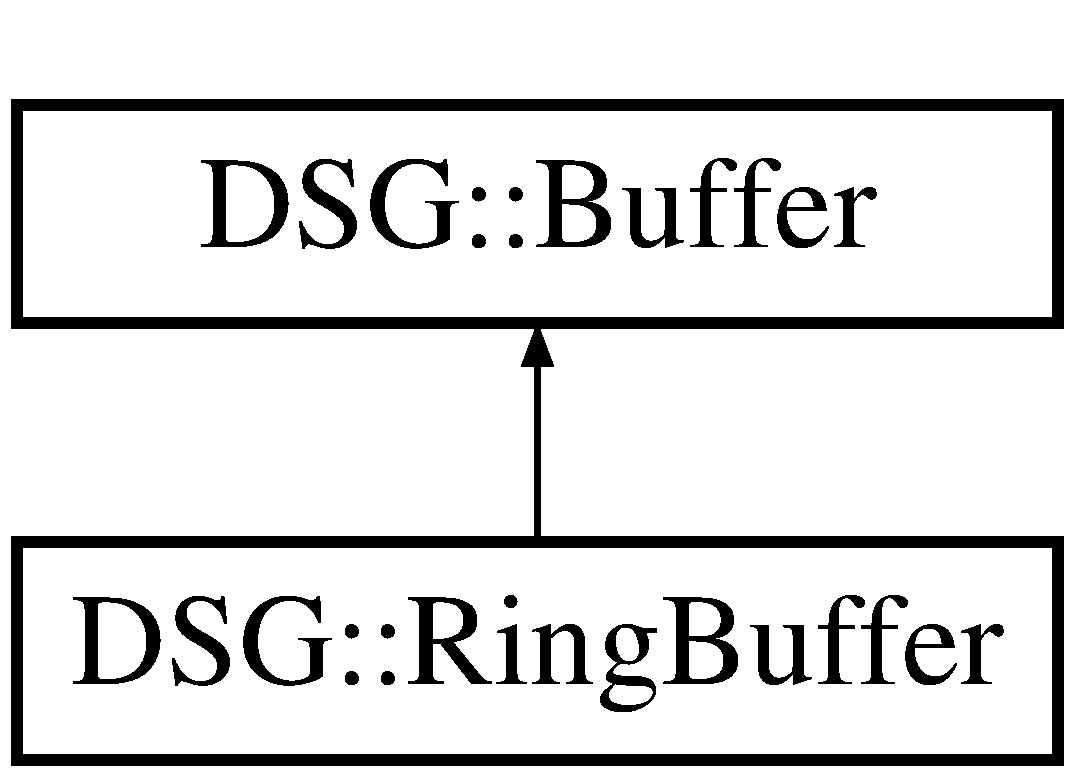
\includegraphics[height=2.000000cm]{classDSG_1_1Buffer}
\end{center}
\end{figure}
\subsection*{Public Member Functions}
\begin{DoxyCompactItemize}
\item 
\hyperlink{classDSG_1_1Buffer_aa764dd8c389dcff51de08cb81fafeb86}{Buffer} ()
\item 
\hyperlink{classDSG_1_1Buffer_a0e6502fd61833043744f9df94e8d5111}{Buffer} (size\+\_\+t size)
\item 
\hyperlink{classDSG_1_1Buffer_a468a65d70553dfb773e4592b4b077683}{Buffer} (\hyperlink{classDSG_1_1Buffer}{Buffer} const \&other)
\item 
\hyperlink{classDSG_1_1Buffer}{Buffer} \& \hyperlink{classDSG_1_1Buffer_a977d572a7d402ff6bf991d7c5c0cc6a7}{operator=} (\hyperlink{classDSG_1_1Buffer}{Buffer} const \&other)
\item 
virtual \hyperlink{classDSG_1_1Buffer_a619fc41bf263a419da1a19254e194101}{$\sim$\+Buffer} ()
\item 
\hyperlink{classDSG_1_1Sample}{Sample} \& \hyperlink{classDSG_1_1Buffer_a5dafe5522f3d20756f83e08499e8eaeb}{operator\mbox{[}$\,$\mbox{]}} (size\+\_\+t const \&index)
\item 
size\+\_\+t const \& \hyperlink{classDSG_1_1Buffer_a4acea659d9cd0be652ec55d21e5b0262}{Size} () const 
\end{DoxyCompactItemize}
\subsection*{Protected Attributes}
\begin{DoxyCompactItemize}
\item 
\hyperlink{classDSG_1_1Sample}{Sample} $\ast$ \hyperlink{classDSG_1_1Buffer_a6506d4763401650acb463cb5d4913e31}{\+\_\+buffer}
\item 
size\+\_\+t \hyperlink{classDSG_1_1Buffer_a4e2fef9ed617af2554b25c999def8f71}{\+\_\+size}
\end{DoxyCompactItemize}


\subsection{Detailed Description}


Definition at line 18 of file Buffer.\+h.



\subsection{Constructor \& Destructor Documentation}
\hypertarget{classDSG_1_1Buffer_aa764dd8c389dcff51de08cb81fafeb86}{\index{D\+S\+G\+::\+Buffer@{D\+S\+G\+::\+Buffer}!Buffer@{Buffer}}
\index{Buffer@{Buffer}!D\+S\+G\+::\+Buffer@{D\+S\+G\+::\+Buffer}}
\subsubsection[{Buffer}]{\setlength{\rightskip}{0pt plus 5cm}D\+S\+G\+::\+Buffer\+::\+Buffer (
\begin{DoxyParamCaption}
{}
\end{DoxyParamCaption}
)}}\label{classDSG_1_1Buffer_aa764dd8c389dcff51de08cb81fafeb86}


Definition at line 13 of file Buffer.\+cpp.


\begin{DoxyCode}
13 :\hyperlink{classDSG_1_1Buffer_a4e2fef9ed617af2554b25c999def8f71}{\_size}(0),\hyperlink{classDSG_1_1Buffer_a6506d4763401650acb463cb5d4913e31}{\_buffer}(\textcolor{keyword}{nullptr})\{\}
\end{DoxyCode}
\hypertarget{classDSG_1_1Buffer_a0e6502fd61833043744f9df94e8d5111}{\index{D\+S\+G\+::\+Buffer@{D\+S\+G\+::\+Buffer}!Buffer@{Buffer}}
\index{Buffer@{Buffer}!D\+S\+G\+::\+Buffer@{D\+S\+G\+::\+Buffer}}
\subsubsection[{Buffer}]{\setlength{\rightskip}{0pt plus 5cm}D\+S\+G\+::\+Buffer\+::\+Buffer (
\begin{DoxyParamCaption}
\item[{size\+\_\+t}]{size}
\end{DoxyParamCaption}
)}}\label{classDSG_1_1Buffer_a0e6502fd61833043744f9df94e8d5111}


Definition at line 14 of file Buffer.\+cpp.


\begin{DoxyCode}
14 :\hyperlink{classDSG_1_1Buffer_a4e2fef9ed617af2554b25c999def8f71}{\_size}(size),\hyperlink{classDSG_1_1Buffer_a6506d4763401650acb463cb5d4913e31}{\_buffer}(\textcolor{keyword}{new}  Sample[size])\{\}
\end{DoxyCode}
\hypertarget{classDSG_1_1Buffer_a468a65d70553dfb773e4592b4b077683}{\index{D\+S\+G\+::\+Buffer@{D\+S\+G\+::\+Buffer}!Buffer@{Buffer}}
\index{Buffer@{Buffer}!D\+S\+G\+::\+Buffer@{D\+S\+G\+::\+Buffer}}
\subsubsection[{Buffer}]{\setlength{\rightskip}{0pt plus 5cm}D\+S\+G\+::\+Buffer\+::\+Buffer (
\begin{DoxyParamCaption}
\item[{{\bf Buffer} const \&}]{other}
\end{DoxyParamCaption}
)}}\label{classDSG_1_1Buffer_a468a65d70553dfb773e4592b4b077683}


Definition at line 15 of file Buffer.\+cpp.


\begin{DoxyCode}
15                                      \{
16     \hyperlink{classDSG_1_1Buffer_a6506d4763401650acb463cb5d4913e31}{\_buffer} = \textcolor{keyword}{new}  Sample[\hyperlink{classDSG_1_1Buffer_a4e2fef9ed617af2554b25c999def8f71}{\_size}];
17     \hyperlink{classDSG_1_1Buffer_a4e2fef9ed617af2554b25c999def8f71}{\_size} = other.\_size;
18     *\textcolor{keyword}{this} = other;
19 \}
\end{DoxyCode}
\hypertarget{classDSG_1_1Buffer_a619fc41bf263a419da1a19254e194101}{\index{D\+S\+G\+::\+Buffer@{D\+S\+G\+::\+Buffer}!````~Buffer@{$\sim$\+Buffer}}
\index{````~Buffer@{$\sim$\+Buffer}!D\+S\+G\+::\+Buffer@{D\+S\+G\+::\+Buffer}}
\subsubsection[{$\sim$\+Buffer}]{\setlength{\rightskip}{0pt plus 5cm}D\+S\+G\+::\+Buffer\+::$\sim$\+Buffer (
\begin{DoxyParamCaption}
{}
\end{DoxyParamCaption}
)\hspace{0.3cm}{\ttfamily [virtual]}}}\label{classDSG_1_1Buffer_a619fc41bf263a419da1a19254e194101}


Definition at line 33 of file Buffer.\+cpp.


\begin{DoxyCode}
33                   \{
34     \textcolor{keywordflow}{if} (\hyperlink{classDSG_1_1Buffer_a6506d4763401650acb463cb5d4913e31}{\_buffer}!=\textcolor{keyword}{nullptr}) \{
35         \textcolor{keyword}{delete} [] \hyperlink{classDSG_1_1Buffer_a6506d4763401650acb463cb5d4913e31}{\_buffer};
36     \}
37 \}
\end{DoxyCode}


\subsection{Member Function Documentation}
\hypertarget{classDSG_1_1Buffer_a977d572a7d402ff6bf991d7c5c0cc6a7}{\index{D\+S\+G\+::\+Buffer@{D\+S\+G\+::\+Buffer}!operator=@{operator=}}
\index{operator=@{operator=}!D\+S\+G\+::\+Buffer@{D\+S\+G\+::\+Buffer}}
\subsubsection[{operator=}]{\setlength{\rightskip}{0pt plus 5cm}{\bf D\+S\+G\+::\+Buffer} \& D\+S\+G\+::\+Buffer\+::operator= (
\begin{DoxyParamCaption}
\item[{{\bf Buffer} const \&}]{other}
\end{DoxyParamCaption}
)}}\label{classDSG_1_1Buffer_a977d572a7d402ff6bf991d7c5c0cc6a7}


Definition at line 20 of file Buffer.\+cpp.


\begin{DoxyCode}
20                                                   \{
21     \textcolor{keywordflow}{if} (\hyperlink{classDSG_1_1Buffer_a4e2fef9ed617af2554b25c999def8f71}{\_size}!=other.\_size) \{
22         \textcolor{keywordflow}{if} (\hyperlink{classDSG_1_1Buffer_a6506d4763401650acb463cb5d4913e31}{\_buffer}!=\textcolor{keyword}{nullptr}) \{
23             \textcolor{keyword}{delete} [] \hyperlink{classDSG_1_1Buffer_a6506d4763401650acb463cb5d4913e31}{\_buffer};
24         \}
25         \hyperlink{classDSG_1_1Buffer_a4e2fef9ed617af2554b25c999def8f71}{\_size} = other.\_size;
26         \hyperlink{classDSG_1_1Buffer_a6506d4763401650acb463cb5d4913e31}{\_buffer} = \textcolor{keyword}{new}  Sample[\hyperlink{classDSG_1_1Buffer_a4e2fef9ed617af2554b25c999def8f71}{\_size}];
27     \}
28     \textcolor{keywordflow}{for} (\textcolor{keywordtype}{int} i=0; i<\hyperlink{classDSG_1_1Buffer_a4e2fef9ed617af2554b25c999def8f71}{\_size}; ++i) \{
29         \hyperlink{classDSG_1_1Buffer_a6506d4763401650acb463cb5d4913e31}{\_buffer}[i] = other.\hyperlink{classDSG_1_1Sample_ab3b67b009491583e03d8e97d579e67c2}{\_buffer}[i];
30     \}
31     \textcolor{keywordflow}{return} *\textcolor{keyword}{this};
32 \}
\end{DoxyCode}
\hypertarget{classDSG_1_1Buffer_a5dafe5522f3d20756f83e08499e8eaeb}{\index{D\+S\+G\+::\+Buffer@{D\+S\+G\+::\+Buffer}!operator\mbox{[}$\,$\mbox{]}@{operator[]}}
\index{operator\mbox{[}$\,$\mbox{]}@{operator[]}!D\+S\+G\+::\+Buffer@{D\+S\+G\+::\+Buffer}}
\subsubsection[{operator[]}]{\setlength{\rightskip}{0pt plus 5cm}{\bf D\+S\+G\+::\+Sample} \& D\+S\+G\+::\+Buffer\+::operator\mbox{[}$\,$\mbox{]} (
\begin{DoxyParamCaption}
\item[{size\+\_\+t const \&}]{index}
\end{DoxyParamCaption}
)}}\label{classDSG_1_1Buffer_a5dafe5522f3d20756f83e08499e8eaeb}


Definition at line 38 of file Buffer.\+cpp.


\begin{DoxyCode}
38                                                     \{
39 \textcolor{preprocessor}{#ifdef DEBUG}
40     assert(index<\hyperlink{classDSG_1_1Buffer_a4e2fef9ed617af2554b25c999def8f71}{\_size});
41 \textcolor{preprocessor}{#endif}
42     \textcolor{keywordflow}{return} \hyperlink{classDSG_1_1Buffer_a6506d4763401650acb463cb5d4913e31}{\_buffer}[index];
43 \}
\end{DoxyCode}
\hypertarget{classDSG_1_1Buffer_a4acea659d9cd0be652ec55d21e5b0262}{\index{D\+S\+G\+::\+Buffer@{D\+S\+G\+::\+Buffer}!Size@{Size}}
\index{Size@{Size}!D\+S\+G\+::\+Buffer@{D\+S\+G\+::\+Buffer}}
\subsubsection[{Size}]{\setlength{\rightskip}{0pt plus 5cm}size\+\_\+t const \& D\+S\+G\+::\+Buffer\+::\+Size (
\begin{DoxyParamCaption}
{}
\end{DoxyParamCaption}
) const\hspace{0.3cm}{\ttfamily [inline]}}}\label{classDSG_1_1Buffer_a4acea659d9cd0be652ec55d21e5b0262}


Definition at line 31 of file Buffer.\+h.


\begin{DoxyCode}
31                                           \{
32         \textcolor{keywordflow}{return} \hyperlink{classDSG_1_1Buffer_a4e2fef9ed617af2554b25c999def8f71}{\_size};
33     \}
\end{DoxyCode}


\subsection{Member Data Documentation}
\hypertarget{classDSG_1_1Buffer_a6506d4763401650acb463cb5d4913e31}{\index{D\+S\+G\+::\+Buffer@{D\+S\+G\+::\+Buffer}!\+\_\+buffer@{\+\_\+buffer}}
\index{\+\_\+buffer@{\+\_\+buffer}!D\+S\+G\+::\+Buffer@{D\+S\+G\+::\+Buffer}}
\subsubsection[{\+\_\+buffer}]{\setlength{\rightskip}{0pt plus 5cm}{\bf Sample}$\ast$ D\+S\+G\+::\+Buffer\+::\+\_\+buffer\hspace{0.3cm}{\ttfamily [protected]}}}\label{classDSG_1_1Buffer_a6506d4763401650acb463cb5d4913e31}


Definition at line 28 of file Buffer.\+h.

\hypertarget{classDSG_1_1Buffer_a4e2fef9ed617af2554b25c999def8f71}{\index{D\+S\+G\+::\+Buffer@{D\+S\+G\+::\+Buffer}!\+\_\+size@{\+\_\+size}}
\index{\+\_\+size@{\+\_\+size}!D\+S\+G\+::\+Buffer@{D\+S\+G\+::\+Buffer}}
\subsubsection[{\+\_\+size}]{\setlength{\rightskip}{0pt plus 5cm}size\+\_\+t D\+S\+G\+::\+Buffer\+::\+\_\+size\hspace{0.3cm}{\ttfamily [protected]}}}\label{classDSG_1_1Buffer_a4e2fef9ed617af2554b25c999def8f71}


Definition at line 29 of file Buffer.\+h.



The documentation for this class was generated from the following files\+:\begin{DoxyCompactItemize}
\item 
/\+Users/alexanderzywicki/\+Documents/\+School\+\_\+\+Stuff/\+Fall\+\_\+2014/\+Digital\+\_\+\+Signal\+\_\+\+Generation\+\_\+and\+\_\+\+Analysis/src/include/\hyperlink{Buffer_8h}{Buffer.\+h}\item 
/\+Users/alexanderzywicki/\+Documents/\+School\+\_\+\+Stuff/\+Fall\+\_\+2014/\+Digital\+\_\+\+Signal\+\_\+\+Generation\+\_\+and\+\_\+\+Analysis/src/\hyperlink{Buffer_8cpp}{Buffer.\+cpp}\end{DoxyCompactItemize}

\hypertarget{classDSG_1_1FourierGenerator}{\section{D\+S\+G\+:\+:Fourier\+Generator Class Reference}
\label{classDSG_1_1FourierGenerator}\index{D\+S\+G\+::\+Fourier\+Generator@{D\+S\+G\+::\+Fourier\+Generator}}
}


A Class Extending The \hyperlink{classDSG_1_1SignalGenerator}{Signal\+Generator} Class with functionality for generating a wave by summing sinusoids.  




{\ttfamily \#include $<$Fourier\+Generator.\+h$>$}

Inheritance diagram for D\+S\+G\+:\+:Fourier\+Generator\+:\begin{figure}[H]
\begin{center}
\leavevmode
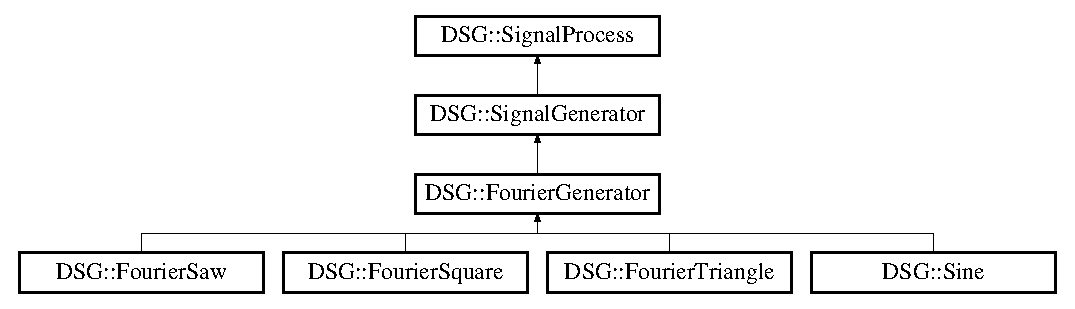
\includegraphics[height=3.708609cm]{classDSG_1_1FourierGenerator}
\end{center}
\end{figure}
\subsection*{Public Member Functions}
\begin{DoxyCompactItemize}
\item 
\hyperlink{classDSG_1_1FourierGenerator_a43fa07fd160c41fd679a5bd2843a5b0e}{Fourier\+Generator} ()
\item 
\hyperlink{classDSG_1_1FourierGenerator_ad3d1099abd1bfedc46f11a5920c0c21b}{Fourier\+Generator} (double const \&frequency, double const \&phase\+\_\+offset)
\item 
virtual \hyperlink{classDSG_1_1FourierGenerator_ab344182f22a7b4d05cbd875a8fa6e40a}{$\sim$\+Fourier\+Generator} ()
\item 
virtual bool \hyperlink{classDSG_1_1FourierGenerator_a7f5e34e65c1fe757318fb5b063dabde9}{Perform} (\hyperlink{classDSG_1_1Sample}{Sample} \&signal)
\item 
virtual bool \hyperlink{classDSG_1_1FourierGenerator_a8b2aca91155dbb524aaf13867f273188}{Perform} (\hyperlink{classDSG_1_1RingBuffer}{Ring\+Buffer} \&signal)
\item 
virtual bool \hyperlink{classDSG_1_1SignalProcess_afdb8220100418893950c1161dd24db67}{Perform} (\hyperlink{classDSG_1_1Sample_aaf2e30d73911eccea99b53eeee15b612}{Sample\+::\+Sample} \&signal)=0
\item 
virtual double const \& \hyperlink{classDSG_1_1SignalGenerator_aedac746c5a70818d120858542ecb7c45}{Frequency} () const 
\item 
virtual double const \& \hyperlink{classDSG_1_1SignalGenerator_ae3ce8d45bafabbd86a0f535b15c3cd46}{Frequency} (double const \&value)
\item 
virtual double const \& \hyperlink{classDSG_1_1SignalGenerator_a1ce521847edd0b837fd840998f906b4b}{Phase\+Offset} () const 
\item 
virtual double const \& \hyperlink{classDSG_1_1SignalGenerator_a08b71b1f30ba65e629642c570291dc0e}{Phase\+Offset} (double const \&value)
\end{DoxyCompactItemize}
\subsection*{Protected Member Functions}
\begin{DoxyCompactItemize}
\item 
unsigned long \hyperlink{classDSG_1_1FourierGenerator_a6b6e3bbad8ff7443d9ed71f4cdf76739}{\+\_\+max\+Harms} (double \+\_\+frq)
\item 
double \hyperlink{classDSG_1_1SignalGenerator_ac0d781b8673b3a283bf7c133290ede50}{\+\_\+pstep} ()
\item 
double \hyperlink{classDSG_1_1SignalGenerator_ae660eb4caa88b8d278f8d24d0908a487}{\+\_\+pstep\+\_\+rad} ()
\item 
void \hyperlink{classDSG_1_1SignalGenerator_a05baccb38d1e52860d4fcf7cb8430efc}{\+\_\+psync} ()
\end{DoxyCompactItemize}
\subsection*{Protected Attributes}
\begin{DoxyCompactItemize}
\item 
\hyperlink{classDSG_1_1Sample}{Sample} \hyperlink{classDSG_1_1FourierGenerator_ab96bed1cd59c42e82a689036e5c62bef}{\+\_\+sample}
\item 
\hyperlink{classDSG_1_1Sample}{Sample} \hyperlink{classDSG_1_1FourierGenerator_a6b7f2439b26914cc9df6b6975a2cedac}{\+\_\+storage}
\item 
double \hyperlink{classDSG_1_1SignalGenerator_aa10f6c85d9adee901139ea7fb346f39d}{\+\_\+rate}
\item 
double \hyperlink{classDSG_1_1SignalGenerator_a67e296e3506dcdf09402c667cddff9ac}{\+\_\+frequency}
\item 
double \hyperlink{classDSG_1_1SignalGenerator_ac2271b582bf699275f077ecb642a8cd9}{\+\_\+phasor}
\end{DoxyCompactItemize}
\subsection*{Static Protected Attributes}
\begin{DoxyCompactItemize}
\item 
static \hyperlink{classDSG_1_1Backend_1_1HarmonicTable}{D\+S\+G\+::\+Backend\+::\+Harmonic\+Table} \hyperlink{classDSG_1_1FourierGenerator_aedac2cf90997418836d064c90540249d}{\+\_\+harmonic\+Table}
\end{DoxyCompactItemize}


\subsection{Detailed Description}
A Class Extending The \hyperlink{classDSG_1_1SignalGenerator}{Signal\+Generator} Class with functionality for generating a wave by summing sinusoids. 

Definition at line 27 of file Fourier\+Generator.\+h.



\subsection{Constructor \& Destructor Documentation}
\hypertarget{classDSG_1_1FourierGenerator_a43fa07fd160c41fd679a5bd2843a5b0e}{\index{D\+S\+G\+::\+Fourier\+Generator@{D\+S\+G\+::\+Fourier\+Generator}!Fourier\+Generator@{Fourier\+Generator}}
\index{Fourier\+Generator@{Fourier\+Generator}!D\+S\+G\+::\+Fourier\+Generator@{D\+S\+G\+::\+Fourier\+Generator}}
\subsubsection[{Fourier\+Generator}]{\setlength{\rightskip}{0pt plus 5cm}D\+S\+G\+::\+Fourier\+Generator\+::\+Fourier\+Generator (
\begin{DoxyParamCaption}
{}
\end{DoxyParamCaption}
)}}\label{classDSG_1_1FourierGenerator_a43fa07fd160c41fd679a5bd2843a5b0e}


Definition at line 12 of file Fourier\+Generator.\+cpp.


\begin{DoxyCode}
12                                      :\hyperlink{classDSG_1_1SignalGenerator_a13ebda67fcdc880ef41aff501cc23fc3}{SignalGenerator}()\{
13     
14 \}
\end{DoxyCode}
\hypertarget{classDSG_1_1FourierGenerator_ad3d1099abd1bfedc46f11a5920c0c21b}{\index{D\+S\+G\+::\+Fourier\+Generator@{D\+S\+G\+::\+Fourier\+Generator}!Fourier\+Generator@{Fourier\+Generator}}
\index{Fourier\+Generator@{Fourier\+Generator}!D\+S\+G\+::\+Fourier\+Generator@{D\+S\+G\+::\+Fourier\+Generator}}
\subsubsection[{Fourier\+Generator}]{\setlength{\rightskip}{0pt plus 5cm}D\+S\+G\+::\+Fourier\+Generator\+::\+Fourier\+Generator (
\begin{DoxyParamCaption}
\item[{double const \&}]{frequency, }
\item[{double const \&}]{phase\+\_\+offset}
\end{DoxyParamCaption}
)}}\label{classDSG_1_1FourierGenerator_ad3d1099abd1bfedc46f11a5920c0c21b}


Definition at line 15 of file Fourier\+Generator.\+cpp.


\begin{DoxyCode}
15 :\hyperlink{classDSG_1_1SignalGenerator_a13ebda67fcdc880ef41aff501cc23fc3}{SignalGenerator}(frequency,phase\_offset)\{\}
\end{DoxyCode}
\hypertarget{classDSG_1_1FourierGenerator_ab344182f22a7b4d05cbd875a8fa6e40a}{\index{D\+S\+G\+::\+Fourier\+Generator@{D\+S\+G\+::\+Fourier\+Generator}!````~Fourier\+Generator@{$\sim$\+Fourier\+Generator}}
\index{````~Fourier\+Generator@{$\sim$\+Fourier\+Generator}!D\+S\+G\+::\+Fourier\+Generator@{D\+S\+G\+::\+Fourier\+Generator}}
\subsubsection[{$\sim$\+Fourier\+Generator}]{\setlength{\rightskip}{0pt plus 5cm}D\+S\+G\+::\+Fourier\+Generator\+::$\sim$\+Fourier\+Generator (
\begin{DoxyParamCaption}
{}
\end{DoxyParamCaption}
)\hspace{0.3cm}{\ttfamily [virtual]}}}\label{classDSG_1_1FourierGenerator_ab344182f22a7b4d05cbd875a8fa6e40a}


Definition at line 16 of file Fourier\+Generator.\+cpp.


\begin{DoxyCode}
16 \{\}
\end{DoxyCode}


\subsection{Member Function Documentation}
\hypertarget{classDSG_1_1FourierGenerator_a6b6e3bbad8ff7443d9ed71f4cdf76739}{\index{D\+S\+G\+::\+Fourier\+Generator@{D\+S\+G\+::\+Fourier\+Generator}!\+\_\+max\+Harms@{\+\_\+max\+Harms}}
\index{\+\_\+max\+Harms@{\+\_\+max\+Harms}!D\+S\+G\+::\+Fourier\+Generator@{D\+S\+G\+::\+Fourier\+Generator}}
\subsubsection[{\+\_\+max\+Harms}]{\setlength{\rightskip}{0pt plus 5cm}unsigned long D\+S\+G\+::\+Fourier\+Generator\+::\+\_\+max\+Harms (
\begin{DoxyParamCaption}
\item[{double}]{\+\_\+frq}
\end{DoxyParamCaption}
)\hspace{0.3cm}{\ttfamily [inline]}, {\ttfamily [protected]}}}\label{classDSG_1_1FourierGenerator_a6b6e3bbad8ff7443d9ed71f4cdf76739}


Definition at line 53 of file Fourier\+Generator.\+h.


\begin{DoxyCode}
53                                                                    \{
54             \textcolor{comment}{//double softLim = 0.45;}
55             \textcolor{comment}{//double hardLim = 0.5;}
56             
57             \textcolor{keywordtype}{double} \_s =  \hyperlink{namespaceDSG_a0c5c3a251b3688398da18138c5efe4bf}{Sample\_Rate}()* (20000.0/ \hyperlink{namespaceDSG_a0c5c3a251b3688398da18138c5efe4bf}{Sample\_Rate}());\textcolor{comment}{//uses harmonic roll
       of based on max human hearing and sample rate}
58             \_s/=\_frq;
59             \textcolor{keywordflow}{return} trunc(\_s);
60         \}
\end{DoxyCode}
\hypertarget{classDSG_1_1SignalGenerator_ac0d781b8673b3a283bf7c133290ede50}{\index{D\+S\+G\+::\+Fourier\+Generator@{D\+S\+G\+::\+Fourier\+Generator}!\+\_\+pstep@{\+\_\+pstep}}
\index{\+\_\+pstep@{\+\_\+pstep}!D\+S\+G\+::\+Fourier\+Generator@{D\+S\+G\+::\+Fourier\+Generator}}
\subsubsection[{\+\_\+pstep}]{\setlength{\rightskip}{0pt plus 5cm}double D\+S\+G\+::\+Signal\+Generator\+::\+\_\+pstep (
\begin{DoxyParamCaption}
{}
\end{DoxyParamCaption}
)\hspace{0.3cm}{\ttfamily [inline]}, {\ttfamily [protected]}, {\ttfamily [inherited]}}}\label{classDSG_1_1SignalGenerator_ac0d781b8673b3a283bf7c133290ede50}


Definition at line 64 of file Signal\+Generator.\+h.


\begin{DoxyCode}
64                                          \{
65         value = \hyperlink{classDSG_1_1SignalGenerator_ac2271b582bf699275f077ecb642a8cd9}{\_phasor};
66         \hyperlink{classDSG_1_1SignalGenerator_ac2271b582bf699275f077ecb642a8cd9}{\_phasor}+=\hyperlink{classDSG_1_1SignalGenerator_aa10f6c85d9adee901139ea7fb346f39d}{\_rate};
67         \hyperlink{classDSG_1_1SignalGenerator_ac2271b582bf699275f077ecb642a8cd9}{\_phasor}>1?\hyperlink{classDSG_1_1SignalGenerator_ac2271b582bf699275f077ecb642a8cd9}{\_phasor}-=1:0;\textcolor{comment}{//cheaper cheaper %1}
68         \textcolor{comment}{//\_phasor -= (unsigned long)\_phasor;//cheaper %1}
69         \textcolor{keywordflow}{return} value;
70     \}
\end{DoxyCode}
\hypertarget{classDSG_1_1SignalGenerator_ae660eb4caa88b8d278f8d24d0908a487}{\index{D\+S\+G\+::\+Fourier\+Generator@{D\+S\+G\+::\+Fourier\+Generator}!\+\_\+pstep\+\_\+rad@{\+\_\+pstep\+\_\+rad}}
\index{\+\_\+pstep\+\_\+rad@{\+\_\+pstep\+\_\+rad}!D\+S\+G\+::\+Fourier\+Generator@{D\+S\+G\+::\+Fourier\+Generator}}
\subsubsection[{\+\_\+pstep\+\_\+rad}]{\setlength{\rightskip}{0pt plus 5cm}double D\+S\+G\+::\+Signal\+Generator\+::\+\_\+pstep\+\_\+rad (
\begin{DoxyParamCaption}
{}
\end{DoxyParamCaption}
)\hspace{0.3cm}{\ttfamily [inline]}, {\ttfamily [protected]}, {\ttfamily [inherited]}}}\label{classDSG_1_1SignalGenerator_ae660eb4caa88b8d278f8d24d0908a487}


Definition at line 71 of file Signal\+Generator.\+h.


\begin{DoxyCode}
71                                              \{
72         \textcolor{keywordflow}{return} \hyperlink{PI_8h_a4912c64aec0c943b7985db6cb61ff83a}{TWOPI} * \hyperlink{classDSG_1_1SignalGenerator_ac0d781b8673b3a283bf7c133290ede50}{\_pstep}();
73     \}
\end{DoxyCode}
\hypertarget{classDSG_1_1SignalGenerator_a05baccb38d1e52860d4fcf7cb8430efc}{\index{D\+S\+G\+::\+Fourier\+Generator@{D\+S\+G\+::\+Fourier\+Generator}!\+\_\+psync@{\+\_\+psync}}
\index{\+\_\+psync@{\+\_\+psync}!D\+S\+G\+::\+Fourier\+Generator@{D\+S\+G\+::\+Fourier\+Generator}}
\subsubsection[{\+\_\+psync}]{\setlength{\rightskip}{0pt plus 5cm}void D\+S\+G\+::\+Signal\+Generator\+::\+\_\+psync (
\begin{DoxyParamCaption}
{}
\end{DoxyParamCaption}
)\hspace{0.3cm}{\ttfamily [inline]}, {\ttfamily [protected]}, {\ttfamily [inherited]}}}\label{classDSG_1_1SignalGenerator_a05baccb38d1e52860d4fcf7cb8430efc}


Definition at line 74 of file Signal\+Generator.\+h.


\begin{DoxyCode}
74                                        \{
75         \hyperlink{classDSG_1_1SignalGenerator_ac2271b582bf699275f077ecb642a8cd9}{\_phasor} = \_phase\_offset;
76     \}
\end{DoxyCode}
\hypertarget{classDSG_1_1SignalGenerator_aedac746c5a70818d120858542ecb7c45}{\index{D\+S\+G\+::\+Fourier\+Generator@{D\+S\+G\+::\+Fourier\+Generator}!Frequency@{Frequency}}
\index{Frequency@{Frequency}!D\+S\+G\+::\+Fourier\+Generator@{D\+S\+G\+::\+Fourier\+Generator}}
\subsubsection[{Frequency}]{\setlength{\rightskip}{0pt plus 5cm}double const \& D\+S\+G\+::\+Signal\+Generator\+::\+Frequency (
\begin{DoxyParamCaption}
{}
\end{DoxyParamCaption}
) const\hspace{0.3cm}{\ttfamily [virtual]}, {\ttfamily [inherited]}}}\label{classDSG_1_1SignalGenerator_aedac746c5a70818d120858542ecb7c45}


Definition at line 16 of file Signal\+Generator.\+cpp.


\begin{DoxyCode}
16                                                 \{
17     \textcolor{keywordflow}{return} \hyperlink{classDSG_1_1SignalGenerator_a67e296e3506dcdf09402c667cddff9ac}{\_frequency};
18 \}
\end{DoxyCode}
\hypertarget{classDSG_1_1SignalGenerator_ae3ce8d45bafabbd86a0f535b15c3cd46}{\index{D\+S\+G\+::\+Fourier\+Generator@{D\+S\+G\+::\+Fourier\+Generator}!Frequency@{Frequency}}
\index{Frequency@{Frequency}!D\+S\+G\+::\+Fourier\+Generator@{D\+S\+G\+::\+Fourier\+Generator}}
\subsubsection[{Frequency}]{\setlength{\rightskip}{0pt plus 5cm}double const \& D\+S\+G\+::\+Signal\+Generator\+::\+Frequency (
\begin{DoxyParamCaption}
\item[{double const \&}]{value}
\end{DoxyParamCaption}
)\hspace{0.3cm}{\ttfamily [virtual]}, {\ttfamily [inherited]}}}\label{classDSG_1_1SignalGenerator_ae3ce8d45bafabbd86a0f535b15c3cd46}


Reimplemented in \hyperlink{classDSG_1_1BLIT_a67b698a54f37c361945cae3e137af76f}{D\+S\+G\+::\+B\+L\+I\+T}, \hyperlink{classDSG_1_1FourierSaw_a929602365c9b29f30f523fa07a29966e}{D\+S\+G\+::\+Fourier\+Saw}, \hyperlink{classDSG_1_1FourierSquare_a80f94eabad633e105cfa673fdee332d6}{D\+S\+G\+::\+Fourier\+Square}, and \hyperlink{classDSG_1_1FourierTriangle_aebb275eee9fb923636a8db5e4aa90b39}{D\+S\+G\+::\+Fourier\+Triangle}.



Definition at line 19 of file Signal\+Generator.\+cpp.


\begin{DoxyCode}
19                                                               \{
20     \hyperlink{classDSG_1_1SignalGenerator_a67e296e3506dcdf09402c667cddff9ac}{\_frequency} = value;
21     \hyperlink{classDSG_1_1SignalGenerator_aa10f6c85d9adee901139ea7fb346f39d}{\_rate} = \hyperlink{classDSG_1_1SignalGenerator_a67e296e3506dcdf09402c667cddff9ac}{\_frequency}/ \hyperlink{namespaceDSG_a0c5c3a251b3688398da18138c5efe4bf}{Sample\_Rate}();
22     \textcolor{keywordflow}{return} \hyperlink{classDSG_1_1SignalGenerator_a67e296e3506dcdf09402c667cddff9ac}{\_frequency};
23 \}
\end{DoxyCode}
\hypertarget{classDSG_1_1SignalProcess_afdb8220100418893950c1161dd24db67}{\index{D\+S\+G\+::\+Fourier\+Generator@{D\+S\+G\+::\+Fourier\+Generator}!Perform@{Perform}}
\index{Perform@{Perform}!D\+S\+G\+::\+Fourier\+Generator@{D\+S\+G\+::\+Fourier\+Generator}}
\subsubsection[{Perform}]{\setlength{\rightskip}{0pt plus 5cm}virtual bool D\+S\+G\+::\+Signal\+Process\+::\+Perform (
\begin{DoxyParamCaption}
\item[{{\bf Sample\+::\+Sample} \&}]{signal}
\end{DoxyParamCaption}
)\hspace{0.3cm}{\ttfamily [inline]}, {\ttfamily [pure virtual]}, {\ttfamily [inherited]}}}\label{classDSG_1_1SignalProcess_afdb8220100418893950c1161dd24db67}
\hypertarget{classDSG_1_1FourierGenerator_a7f5e34e65c1fe757318fb5b063dabde9}{\index{D\+S\+G\+::\+Fourier\+Generator@{D\+S\+G\+::\+Fourier\+Generator}!Perform@{Perform}}
\index{Perform@{Perform}!D\+S\+G\+::\+Fourier\+Generator@{D\+S\+G\+::\+Fourier\+Generator}}
\subsubsection[{Perform}]{\setlength{\rightskip}{0pt plus 5cm}bool D\+S\+G\+::\+Fourier\+Generator\+::\+Perform (
\begin{DoxyParamCaption}
\item[{{\bf Sample} \&}]{signal}
\end{DoxyParamCaption}
)\hspace{0.3cm}{\ttfamily [inline]}, {\ttfamily [virtual]}}}\label{classDSG_1_1FourierGenerator_a7f5e34e65c1fe757318fb5b063dabde9}


Reimplemented from \hyperlink{classDSG_1_1SignalGenerator_a95d485b68d874938ac93644b121607b9}{D\+S\+G\+::\+Signal\+Generator}.



Reimplemented in \hyperlink{classDSG_1_1FourierSaw_a3cc372cd7dd694f8b9cb70e504dd04a1}{D\+S\+G\+::\+Fourier\+Saw}, \hyperlink{classDSG_1_1FourierSquare_a3e9cfc95b3592eaf04fbcd61a3c68387}{D\+S\+G\+::\+Fourier\+Square}, \hyperlink{classDSG_1_1FourierTriangle_ae927efb96f8d40f620dd02bdaaeef4d5}{D\+S\+G\+::\+Fourier\+Triangle}, and \hyperlink{classDSG_1_1Sine_a04d925dc8c9a4b320f21697ce853a407}{D\+S\+G\+::\+Sine}.



Definition at line 43 of file Fourier\+Generator.\+h.


\begin{DoxyCode}
43                                                             \{
44             signal = 0;
45             \textcolor{keywordflow}{return} \textcolor{keyword}{false};
46         \}
\end{DoxyCode}
\hypertarget{classDSG_1_1FourierGenerator_a8b2aca91155dbb524aaf13867f273188}{\index{D\+S\+G\+::\+Fourier\+Generator@{D\+S\+G\+::\+Fourier\+Generator}!Perform@{Perform}}
\index{Perform@{Perform}!D\+S\+G\+::\+Fourier\+Generator@{D\+S\+G\+::\+Fourier\+Generator}}
\subsubsection[{Perform}]{\setlength{\rightskip}{0pt plus 5cm}bool D\+S\+G\+::\+Fourier\+Generator\+::\+Perform (
\begin{DoxyParamCaption}
\item[{{\bf Ring\+Buffer} \&}]{signal}
\end{DoxyParamCaption}
)\hspace{0.3cm}{\ttfamily [inline]}, {\ttfamily [virtual]}}}\label{classDSG_1_1FourierGenerator_a8b2aca91155dbb524aaf13867f273188}


Reimplemented from \hyperlink{classDSG_1_1SignalGenerator_abaa9aecd00b792d46166b91524b42db6}{D\+S\+G\+::\+Signal\+Generator}.



Reimplemented in \hyperlink{classDSG_1_1FourierSaw_a76b78874feebbc89d00656fec4bfd57a}{D\+S\+G\+::\+Fourier\+Saw}, \hyperlink{classDSG_1_1FourierSquare_ad9999119d9efc453329ed4b3eaf5f226}{D\+S\+G\+::\+Fourier\+Square}, \hyperlink{classDSG_1_1FourierTriangle_a017e2b59123ff3afa9a5c0e833e5f482}{D\+S\+G\+::\+Fourier\+Triangle}, and \hyperlink{classDSG_1_1Sine_a6408fedf61f1f2a4026261d181997afc}{D\+S\+G\+::\+Sine}.



Definition at line 47 of file Fourier\+Generator.\+h.


\begin{DoxyCode}
47                                                                 \{
48             signal.Flush();
49             \textcolor{keywordflow}{return} \textcolor{keyword}{false};
50         \}
\end{DoxyCode}
\hypertarget{classDSG_1_1SignalGenerator_a1ce521847edd0b837fd840998f906b4b}{\index{D\+S\+G\+::\+Fourier\+Generator@{D\+S\+G\+::\+Fourier\+Generator}!Phase\+Offset@{Phase\+Offset}}
\index{Phase\+Offset@{Phase\+Offset}!D\+S\+G\+::\+Fourier\+Generator@{D\+S\+G\+::\+Fourier\+Generator}}
\subsubsection[{Phase\+Offset}]{\setlength{\rightskip}{0pt plus 5cm}double const \& D\+S\+G\+::\+Signal\+Generator\+::\+Phase\+Offset (
\begin{DoxyParamCaption}
{}
\end{DoxyParamCaption}
) const\hspace{0.3cm}{\ttfamily [virtual]}, {\ttfamily [inherited]}}}\label{classDSG_1_1SignalGenerator_a1ce521847edd0b837fd840998f906b4b}


Definition at line 24 of file Signal\+Generator.\+cpp.


\begin{DoxyCode}
24                                                   \{
25     \textcolor{keywordflow}{return} \_phase\_offset;
26 \}
\end{DoxyCode}
\hypertarget{classDSG_1_1SignalGenerator_a08b71b1f30ba65e629642c570291dc0e}{\index{D\+S\+G\+::\+Fourier\+Generator@{D\+S\+G\+::\+Fourier\+Generator}!Phase\+Offset@{Phase\+Offset}}
\index{Phase\+Offset@{Phase\+Offset}!D\+S\+G\+::\+Fourier\+Generator@{D\+S\+G\+::\+Fourier\+Generator}}
\subsubsection[{Phase\+Offset}]{\setlength{\rightskip}{0pt plus 5cm}double const \& D\+S\+G\+::\+Signal\+Generator\+::\+Phase\+Offset (
\begin{DoxyParamCaption}
\item[{double const \&}]{value}
\end{DoxyParamCaption}
)\hspace{0.3cm}{\ttfamily [virtual]}, {\ttfamily [inherited]}}}\label{classDSG_1_1SignalGenerator_a08b71b1f30ba65e629642c570291dc0e}


Definition at line 27 of file Signal\+Generator.\+cpp.


\begin{DoxyCode}
27                                                                 \{
28     \_phase\_offset-=value;
29     \hyperlink{classDSG_1_1SignalGenerator_ac2271b582bf699275f077ecb642a8cd9}{\_phasor}-=\_phase\_offset;
30     \_phase\_offset=value;
31     \textcolor{keywordflow}{return} \_phase\_offset;
32 \}
\end{DoxyCode}


\subsection{Member Data Documentation}
\hypertarget{classDSG_1_1SignalGenerator_a67e296e3506dcdf09402c667cddff9ac}{\index{D\+S\+G\+::\+Fourier\+Generator@{D\+S\+G\+::\+Fourier\+Generator}!\+\_\+frequency@{\+\_\+frequency}}
\index{\+\_\+frequency@{\+\_\+frequency}!D\+S\+G\+::\+Fourier\+Generator@{D\+S\+G\+::\+Fourier\+Generator}}
\subsubsection[{\+\_\+frequency}]{\setlength{\rightskip}{0pt plus 5cm}double D\+S\+G\+::\+Signal\+Generator\+::\+\_\+frequency\hspace{0.3cm}{\ttfamily [protected]}, {\ttfamily [inherited]}}}\label{classDSG_1_1SignalGenerator_a67e296e3506dcdf09402c667cddff9ac}


Definition at line 34 of file Signal\+Generator.\+h.

\hypertarget{classDSG_1_1FourierGenerator_aedac2cf90997418836d064c90540249d}{\index{D\+S\+G\+::\+Fourier\+Generator@{D\+S\+G\+::\+Fourier\+Generator}!\+\_\+harmonic\+Table@{\+\_\+harmonic\+Table}}
\index{\+\_\+harmonic\+Table@{\+\_\+harmonic\+Table}!D\+S\+G\+::\+Fourier\+Generator@{D\+S\+G\+::\+Fourier\+Generator}}
\subsubsection[{\+\_\+harmonic\+Table}]{\setlength{\rightskip}{0pt plus 5cm}{\bf D\+S\+G\+::\+Backend\+::\+Harmonic\+Table} D\+S\+G\+::\+Fourier\+Generator\+::\+\_\+harmonic\+Table\hspace{0.3cm}{\ttfamily [static]}, {\ttfamily [protected]}}}\label{classDSG_1_1FourierGenerator_aedac2cf90997418836d064c90540249d}


Definition at line 39 of file Fourier\+Generator.\+h.

\hypertarget{classDSG_1_1SignalGenerator_ac2271b582bf699275f077ecb642a8cd9}{\index{D\+S\+G\+::\+Fourier\+Generator@{D\+S\+G\+::\+Fourier\+Generator}!\+\_\+phasor@{\+\_\+phasor}}
\index{\+\_\+phasor@{\+\_\+phasor}!D\+S\+G\+::\+Fourier\+Generator@{D\+S\+G\+::\+Fourier\+Generator}}
\subsubsection[{\+\_\+phasor}]{\setlength{\rightskip}{0pt plus 5cm}double D\+S\+G\+::\+Signal\+Generator\+::\+\_\+phasor\hspace{0.3cm}{\ttfamily [protected]}, {\ttfamily [inherited]}}}\label{classDSG_1_1SignalGenerator_ac2271b582bf699275f077ecb642a8cd9}


Definition at line 46 of file Signal\+Generator.\+h.

\hypertarget{classDSG_1_1SignalGenerator_aa10f6c85d9adee901139ea7fb346f39d}{\index{D\+S\+G\+::\+Fourier\+Generator@{D\+S\+G\+::\+Fourier\+Generator}!\+\_\+rate@{\+\_\+rate}}
\index{\+\_\+rate@{\+\_\+rate}!D\+S\+G\+::\+Fourier\+Generator@{D\+S\+G\+::\+Fourier\+Generator}}
\subsubsection[{\+\_\+rate}]{\setlength{\rightskip}{0pt plus 5cm}double D\+S\+G\+::\+Signal\+Generator\+::\+\_\+rate\hspace{0.3cm}{\ttfamily [protected]}, {\ttfamily [inherited]}}}\label{classDSG_1_1SignalGenerator_aa10f6c85d9adee901139ea7fb346f39d}


Definition at line 33 of file Signal\+Generator.\+h.

\hypertarget{classDSG_1_1FourierGenerator_ab96bed1cd59c42e82a689036e5c62bef}{\index{D\+S\+G\+::\+Fourier\+Generator@{D\+S\+G\+::\+Fourier\+Generator}!\+\_\+sample@{\+\_\+sample}}
\index{\+\_\+sample@{\+\_\+sample}!D\+S\+G\+::\+Fourier\+Generator@{D\+S\+G\+::\+Fourier\+Generator}}
\subsubsection[{\+\_\+sample}]{\setlength{\rightskip}{0pt plus 5cm}{\bf Sample} D\+S\+G\+::\+Fourier\+Generator\+::\+\_\+sample\hspace{0.3cm}{\ttfamily [protected]}}}\label{classDSG_1_1FourierGenerator_ab96bed1cd59c42e82a689036e5c62bef}


Definition at line 37 of file Fourier\+Generator.\+h.

\hypertarget{classDSG_1_1FourierGenerator_a6b7f2439b26914cc9df6b6975a2cedac}{\index{D\+S\+G\+::\+Fourier\+Generator@{D\+S\+G\+::\+Fourier\+Generator}!\+\_\+storage@{\+\_\+storage}}
\index{\+\_\+storage@{\+\_\+storage}!D\+S\+G\+::\+Fourier\+Generator@{D\+S\+G\+::\+Fourier\+Generator}}
\subsubsection[{\+\_\+storage}]{\setlength{\rightskip}{0pt plus 5cm}{\bf Sample} D\+S\+G\+::\+Fourier\+Generator\+::\+\_\+storage\hspace{0.3cm}{\ttfamily [protected]}}}\label{classDSG_1_1FourierGenerator_a6b7f2439b26914cc9df6b6975a2cedac}


Definition at line 38 of file Fourier\+Generator.\+h.



The documentation for this class was generated from the following files\+:\begin{DoxyCompactItemize}
\item 
/\+Users/alexanderzywicki/\+Documents/\+School\+\_\+\+Stuff/\+Fall\+\_\+2014/\+Digital\+\_\+\+Signal\+\_\+\+Generation\+\_\+and\+\_\+\+Analysis/src/include/\hyperlink{FourierGenerator_8h}{Fourier\+Generator.\+h}\item 
/\+Users/alexanderzywicki/\+Documents/\+School\+\_\+\+Stuff/\+Fall\+\_\+2014/\+Digital\+\_\+\+Signal\+\_\+\+Generation\+\_\+and\+\_\+\+Analysis/src/\hyperlink{FourierGenerator_8cpp}{Fourier\+Generator.\+cpp}\end{DoxyCompactItemize}

\hypertarget{classDSG_1_1FourierSaw}{\section{D\+S\+G\+:\+:Fourier\+Saw Class Reference}
\label{classDSG_1_1FourierSaw}\index{D\+S\+G\+::\+Fourier\+Saw@{D\+S\+G\+::\+Fourier\+Saw}}
}


Fourier Series Based Saw Wave.  




{\ttfamily \#include $<$Fourier\+Saw.\+h$>$}

Inheritance diagram for D\+S\+G\+:\+:Fourier\+Saw\+:\begin{figure}[H]
\begin{center}
\leavevmode
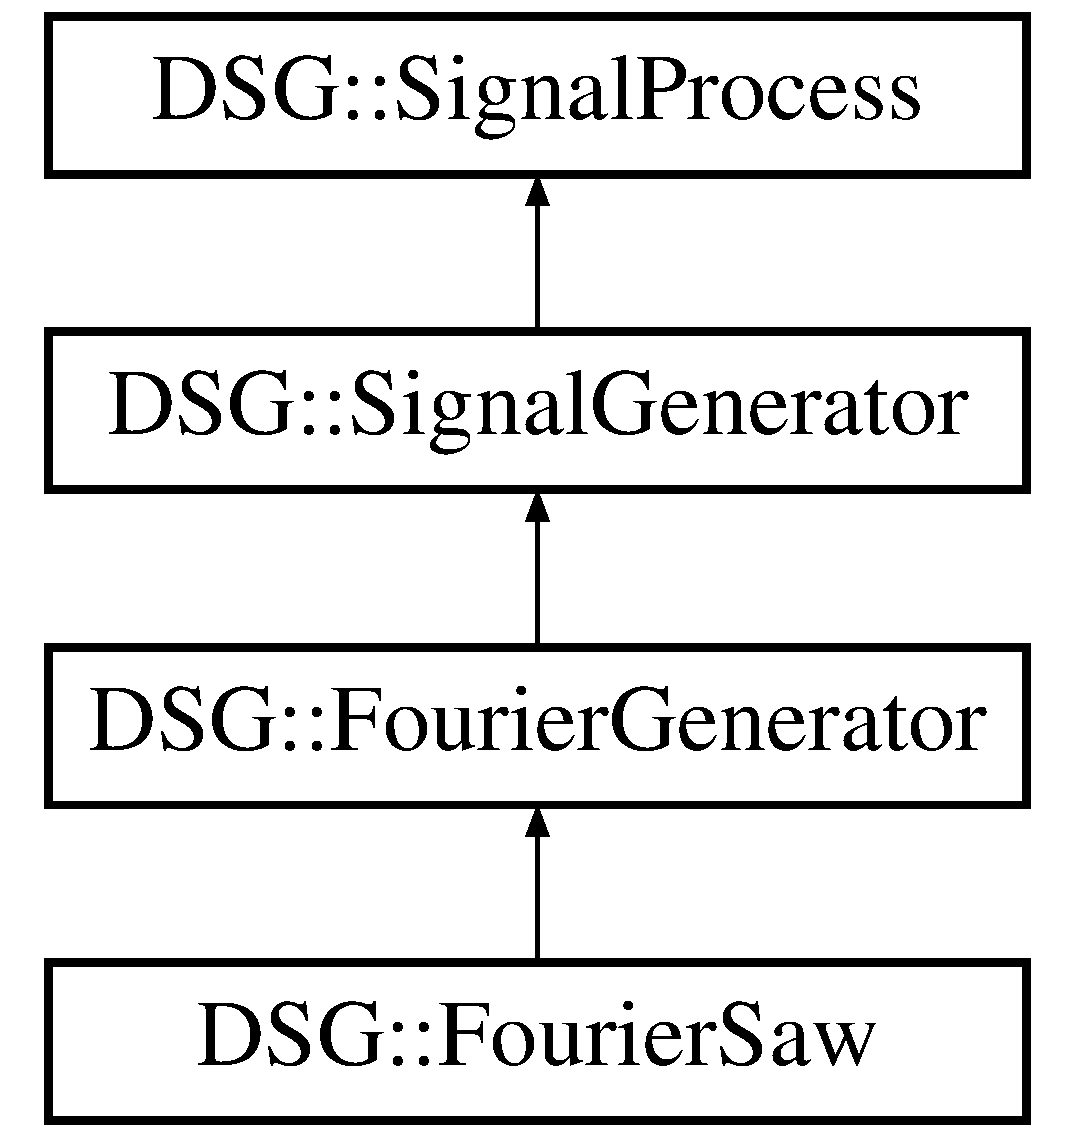
\includegraphics[height=4.000000cm]{classDSG_1_1FourierSaw}
\end{center}
\end{figure}
\subsection*{Public Member Functions}
\begin{DoxyCompactItemize}
\item 
\hyperlink{classDSG_1_1FourierSaw_ac4d5bde5f7ed868abda94cffe32ce4cb}{Fourier\+Saw} ()
\item 
\hyperlink{classDSG_1_1FourierSaw_a9a0bc3906f29e8967da69287012d90d3}{Fourier\+Saw} (double const \&frequency, double const \&phase\+\_\+offset)
\item 
virtual \hyperlink{classDSG_1_1FourierSaw_aa542b5b69e4046fcf0c48f052cb5975d}{$\sim$\+Fourier\+Saw} ()
\item 
virtual bool \hyperlink{classDSG_1_1FourierSaw_a3cc372cd7dd694f8b9cb70e504dd04a1}{Perform} (\hyperlink{classDSG_1_1Sample}{Sample} \&signal)
\item 
virtual bool \hyperlink{classDSG_1_1FourierSaw_a76b78874feebbc89d00656fec4bfd57a}{Perform} (\hyperlink{classDSG_1_1RingBuffer}{Ring\+Buffer} \&signal)
\item 
virtual double const \& \hyperlink{classDSG_1_1FourierSaw_a929602365c9b29f30f523fa07a29966e}{Frequency} (double const \&value)
\item 
virtual double const \& \hyperlink{classDSG_1_1FourierSaw_a427afe0a006b15ebbd29076a12946c55}{Frequency} ()
\item 
virtual bool \hyperlink{classDSG_1_1SignalProcess_afdb8220100418893950c1161dd24db67}{Perform} (\hyperlink{classDSG_1_1Sample_aaf2e30d73911eccea99b53eeee15b612}{Sample\+::\+Sample} \&signal)=0
\item 
virtual double const \& \hyperlink{classDSG_1_1SignalGenerator_aedac746c5a70818d120858542ecb7c45}{Frequency} () const 
\item 
virtual double const \& \hyperlink{classDSG_1_1SignalGenerator_a1ce521847edd0b837fd840998f906b4b}{Phase\+Offset} () const 
\item 
virtual double const \& \hyperlink{classDSG_1_1SignalGenerator_a08b71b1f30ba65e629642c570291dc0e}{Phase\+Offset} (double const \&value)
\end{DoxyCompactItemize}
\subsection*{Protected Member Functions}
\begin{DoxyCompactItemize}
\item 
unsigned long \hyperlink{classDSG_1_1FourierGenerator_a6b6e3bbad8ff7443d9ed71f4cdf76739}{\+\_\+max\+Harms} (double \+\_\+frq)
\item 
double \hyperlink{classDSG_1_1SignalGenerator_ac0d781b8673b3a283bf7c133290ede50}{\+\_\+pstep} ()
\item 
double \hyperlink{classDSG_1_1SignalGenerator_ae660eb4caa88b8d278f8d24d0908a487}{\+\_\+pstep\+\_\+rad} ()
\item 
void \hyperlink{classDSG_1_1SignalGenerator_a05baccb38d1e52860d4fcf7cb8430efc}{\+\_\+psync} ()
\end{DoxyCompactItemize}
\subsection*{Protected Attributes}
\begin{DoxyCompactItemize}
\item 
unsigned long \hyperlink{classDSG_1_1FourierSaw_afaa437e6dda9ddbd4f011012dfe3c55a}{\+\_\+h}
\item 
float \hyperlink{classDSG_1_1FourierSaw_a44f77f54a92eb8bc1fe3d116bdb01e5f}{\+\_\+a}
\item 
float \hyperlink{classDSG_1_1FourierSaw_a8e8c9940318ca36eb5f10a8c5dfa6264}{phs}
\item 
float \hyperlink{classDSG_1_1FourierSaw_ae4fd4aba08605f9a7934831b6c171027}{stor}
\item 
float \hyperlink{classDSG_1_1FourierSaw_afc22691229a12cd83726f09634d60d3b}{\+\_\+tmp}
\item 
float \hyperlink{classDSG_1_1FourierSaw_a862f4353823d0d1fb26355a4aaeced3a}{i\+P\+I}
\item 
float \hyperlink{classDSG_1_1FourierSaw_a23bf3488fcdfb556df02d8cf0103e30f}{\+\_\+param}
\item 
unsigned short \hyperlink{classDSG_1_1FourierSaw_ad4fecfc1b1500bc514fb2d9e794ef411}{i}
\item 
\hyperlink{classDSG_1_1Sample}{Sample} \hyperlink{classDSG_1_1FourierGenerator_ab96bed1cd59c42e82a689036e5c62bef}{\+\_\+sample}
\item 
\hyperlink{classDSG_1_1Sample}{Sample} \hyperlink{classDSG_1_1FourierGenerator_a6b7f2439b26914cc9df6b6975a2cedac}{\+\_\+storage}
\item 
double \hyperlink{classDSG_1_1SignalGenerator_aa10f6c85d9adee901139ea7fb346f39d}{\+\_\+rate}
\item 
double \hyperlink{classDSG_1_1SignalGenerator_a67e296e3506dcdf09402c667cddff9ac}{\+\_\+frequency}
\item 
double \hyperlink{classDSG_1_1SignalGenerator_ac2271b582bf699275f077ecb642a8cd9}{\+\_\+phasor}
\end{DoxyCompactItemize}
\subsection*{Static Protected Attributes}
\begin{DoxyCompactItemize}
\item 
static \hyperlink{classDSG_1_1HarmonicTable}{D\+S\+G\+::\+Harmonic\+Table} \hyperlink{classDSG_1_1FourierGenerator_a7288408f8e44d5edb5eecc62480243d7}{\+\_\+harmonic\+Table}
\item 
static \hyperlink{classDSG_1_1SineLUT}{D\+S\+G\+::\+Sine\+L\+U\+T}$<$ float, 32768 $>$ \hyperlink{classDSG_1_1FourierGenerator_a1ae5fb243ce05e638bdf0dec8bde7426}{\+\_\+sine\+Lut}
\end{DoxyCompactItemize}


\subsection{Detailed Description}
Fourier Series Based Saw Wave. 

Definition at line 16 of file Fourier\+Saw.\+h.



\subsection{Constructor \& Destructor Documentation}
\hypertarget{classDSG_1_1FourierSaw_ac4d5bde5f7ed868abda94cffe32ce4cb}{\index{D\+S\+G\+::\+Fourier\+Saw@{D\+S\+G\+::\+Fourier\+Saw}!Fourier\+Saw@{Fourier\+Saw}}
\index{Fourier\+Saw@{Fourier\+Saw}!D\+S\+G\+::\+Fourier\+Saw@{D\+S\+G\+::\+Fourier\+Saw}}
\subsubsection[{Fourier\+Saw}]{\setlength{\rightskip}{0pt plus 5cm}D\+S\+G\+::\+Fourier\+Saw\+::\+Fourier\+Saw (
\begin{DoxyParamCaption}
{}
\end{DoxyParamCaption}
)}}\label{classDSG_1_1FourierSaw_ac4d5bde5f7ed868abda94cffe32ce4cb}


Definition at line 10 of file Fourier\+Saw.\+cpp.


\begin{DoxyCode}
10                          :\hyperlink{classDSG_1_1FourierGenerator_a43fa07fd160c41fd679a5bd2843a5b0e}{FourierGenerator}(),\hyperlink{classDSG_1_1FourierSaw_a44f77f54a92eb8bc1fe3d116bdb01e5f}{\_a}(3.6/3.0),\hyperlink{classDSG_1_1FourierSaw_afaa437e6dda9ddbd4f011012dfe3c55a}{\_h}(
      \hyperlink{classDSG_1_1FourierGenerator_a6b6e3bbad8ff7443d9ed71f4cdf76739}{\_maxHarms}(\hyperlink{classDSG_1_1SignalGenerator_a67e296e3506dcdf09402c667cddff9ac}{\_frequency})+1),\hyperlink{classDSG_1_1FourierSaw_a862f4353823d0d1fb26355a4aaeced3a}{iPI}(1.0/\hyperlink{PI_8h_a598a3330b3c21701223ee0ca14316eca}{PI}),\hyperlink{classDSG_1_1FourierSaw_a8e8c9940318ca36eb5f10a8c5dfa6264}{phs}(0),\hyperlink{classDSG_1_1FourierSaw_ae4fd4aba08605f9a7934831b6c171027}{stor}(0),
      \hyperlink{classDSG_1_1FourierSaw_afc22691229a12cd83726f09634d60d3b}{\_tmp}(0)\{
11     \hyperlink{classDSG_1_1FourierSaw_a44f77f54a92eb8bc1fe3d116bdb01e5f}{\_a}*=\hyperlink{classDSG_1_1FourierSaw_a862f4353823d0d1fb26355a4aaeced3a}{iPI};
12 \}
\end{DoxyCode}
\hypertarget{classDSG_1_1FourierSaw_a9a0bc3906f29e8967da69287012d90d3}{\index{D\+S\+G\+::\+Fourier\+Saw@{D\+S\+G\+::\+Fourier\+Saw}!Fourier\+Saw@{Fourier\+Saw}}
\index{Fourier\+Saw@{Fourier\+Saw}!D\+S\+G\+::\+Fourier\+Saw@{D\+S\+G\+::\+Fourier\+Saw}}
\subsubsection[{Fourier\+Saw}]{\setlength{\rightskip}{0pt plus 5cm}D\+S\+G\+::\+Fourier\+Saw\+::\+Fourier\+Saw (
\begin{DoxyParamCaption}
\item[{double const \&}]{frequency, }
\item[{double const \&}]{phase\+\_\+offset}
\end{DoxyParamCaption}
)}}\label{classDSG_1_1FourierSaw_a9a0bc3906f29e8967da69287012d90d3}


Definition at line 13 of file Fourier\+Saw.\+cpp.


\begin{DoxyCode}
13                                                                            :
      \hyperlink{classDSG_1_1FourierGenerator_a43fa07fd160c41fd679a5bd2843a5b0e}{FourierGenerator}(frequency,phase\_offset),\hyperlink{classDSG_1_1FourierSaw_a44f77f54a92eb8bc1fe3d116bdb01e5f}{\_a}(3.6/3.0),\hyperlink{classDSG_1_1FourierSaw_afaa437e6dda9ddbd4f011012dfe3c55a}{\_h}(
      \hyperlink{classDSG_1_1FourierGenerator_a6b6e3bbad8ff7443d9ed71f4cdf76739}{\_maxHarms}(\hyperlink{classDSG_1_1SignalGenerator_a67e296e3506dcdf09402c667cddff9ac}{\_frequency})+1),\hyperlink{classDSG_1_1FourierSaw_a862f4353823d0d1fb26355a4aaeced3a}{iPI}(1.0/\hyperlink{PI_8h_a598a3330b3c21701223ee0ca14316eca}{PI}),\hyperlink{classDSG_1_1FourierSaw_a8e8c9940318ca36eb5f10a8c5dfa6264}{phs}(0),\hyperlink{classDSG_1_1FourierSaw_ae4fd4aba08605f9a7934831b6c171027}{stor}(0),
      \hyperlink{classDSG_1_1FourierSaw_afc22691229a12cd83726f09634d60d3b}{\_tmp}(0)\{
14     \hyperlink{classDSG_1_1FourierGenerator_ab96bed1cd59c42e82a689036e5c62bef}{\_sample}=0;
15     \hyperlink{classDSG_1_1FourierGenerator_a6b7f2439b26914cc9df6b6975a2cedac}{\_storage}=0;
16     \hyperlink{classDSG_1_1FourierSaw_a44f77f54a92eb8bc1fe3d116bdb01e5f}{\_a}*=\hyperlink{classDSG_1_1FourierSaw_a862f4353823d0d1fb26355a4aaeced3a}{iPI};
17 \}
\end{DoxyCode}
\hypertarget{classDSG_1_1FourierSaw_aa542b5b69e4046fcf0c48f052cb5975d}{\index{D\+S\+G\+::\+Fourier\+Saw@{D\+S\+G\+::\+Fourier\+Saw}!````~Fourier\+Saw@{$\sim$\+Fourier\+Saw}}
\index{````~Fourier\+Saw@{$\sim$\+Fourier\+Saw}!D\+S\+G\+::\+Fourier\+Saw@{D\+S\+G\+::\+Fourier\+Saw}}
\subsubsection[{$\sim$\+Fourier\+Saw}]{\setlength{\rightskip}{0pt plus 5cm}D\+S\+G\+::\+Fourier\+Saw\+::$\sim$\+Fourier\+Saw (
\begin{DoxyParamCaption}
{}
\end{DoxyParamCaption}
)\hspace{0.3cm}{\ttfamily [virtual]}}}\label{classDSG_1_1FourierSaw_aa542b5b69e4046fcf0c48f052cb5975d}


Definition at line 18 of file Fourier\+Saw.\+cpp.


\begin{DoxyCode}
18 \{\}
\end{DoxyCode}


\subsection{Member Function Documentation}
\hypertarget{classDSG_1_1FourierGenerator_a6b6e3bbad8ff7443d9ed71f4cdf76739}{\index{D\+S\+G\+::\+Fourier\+Saw@{D\+S\+G\+::\+Fourier\+Saw}!\+\_\+max\+Harms@{\+\_\+max\+Harms}}
\index{\+\_\+max\+Harms@{\+\_\+max\+Harms}!D\+S\+G\+::\+Fourier\+Saw@{D\+S\+G\+::\+Fourier\+Saw}}
\subsubsection[{\+\_\+max\+Harms}]{\setlength{\rightskip}{0pt plus 5cm}unsigned long D\+S\+G\+::\+Fourier\+Generator\+::\+\_\+max\+Harms (
\begin{DoxyParamCaption}
\item[{double}]{\+\_\+frq}
\end{DoxyParamCaption}
)\hspace{0.3cm}{\ttfamily [inline]}, {\ttfamily [protected]}, {\ttfamily [inherited]}}}\label{classDSG_1_1FourierGenerator_a6b6e3bbad8ff7443d9ed71f4cdf76739}


Definition at line 45 of file Fourier\+Generator.\+h.


\begin{DoxyCode}
45                                                                    \{
46             \textcolor{comment}{//double softLim = 0.45;}
47             \textcolor{comment}{//double hardLim = 0.5;}
48             
49             \textcolor{keywordtype}{double} \_s =  \hyperlink{namespaceDSG_a0c5c3a251b3688398da18138c5efe4bf}{Sample\_Rate}()* (20000.0/ \hyperlink{namespaceDSG_a0c5c3a251b3688398da18138c5efe4bf}{Sample\_Rate}());\textcolor{comment}{//uses harmonic roll
       of based on max human hearing and sample rate}
50             \_s/=\_frq;
51             \textcolor{keywordflow}{return} trunc(\_s);
52         \}
\end{DoxyCode}
\hypertarget{classDSG_1_1SignalGenerator_ac0d781b8673b3a283bf7c133290ede50}{\index{D\+S\+G\+::\+Fourier\+Saw@{D\+S\+G\+::\+Fourier\+Saw}!\+\_\+pstep@{\+\_\+pstep}}
\index{\+\_\+pstep@{\+\_\+pstep}!D\+S\+G\+::\+Fourier\+Saw@{D\+S\+G\+::\+Fourier\+Saw}}
\subsubsection[{\+\_\+pstep}]{\setlength{\rightskip}{0pt plus 5cm}double D\+S\+G\+::\+Signal\+Generator\+::\+\_\+pstep (
\begin{DoxyParamCaption}
{}
\end{DoxyParamCaption}
)\hspace{0.3cm}{\ttfamily [inline]}, {\ttfamily [protected]}, {\ttfamily [inherited]}}}\label{classDSG_1_1SignalGenerator_ac0d781b8673b3a283bf7c133290ede50}


Definition at line 52 of file Signal\+Generator.\+h.


\begin{DoxyCode}
52                                          \{
53         value = \hyperlink{classDSG_1_1SignalGenerator_ac2271b582bf699275f077ecb642a8cd9}{\_phasor};
54         \hyperlink{classDSG_1_1SignalGenerator_ac2271b582bf699275f077ecb642a8cd9}{\_phasor}+=\hyperlink{classDSG_1_1SignalGenerator_aa10f6c85d9adee901139ea7fb346f39d}{\_rate};
55         \hyperlink{classDSG_1_1SignalGenerator_ac2271b582bf699275f077ecb642a8cd9}{\_phasor}>1?\hyperlink{classDSG_1_1SignalGenerator_ac2271b582bf699275f077ecb642a8cd9}{\_phasor}-=1:0;\textcolor{comment}{//cheaper cheaper %1}
56         \textcolor{comment}{//\_phasor -= (unsigned long)\_phasor;//cheaper %1}
57         \textcolor{keywordflow}{return} value;
58     \}
\end{DoxyCode}
\hypertarget{classDSG_1_1SignalGenerator_ae660eb4caa88b8d278f8d24d0908a487}{\index{D\+S\+G\+::\+Fourier\+Saw@{D\+S\+G\+::\+Fourier\+Saw}!\+\_\+pstep\+\_\+rad@{\+\_\+pstep\+\_\+rad}}
\index{\+\_\+pstep\+\_\+rad@{\+\_\+pstep\+\_\+rad}!D\+S\+G\+::\+Fourier\+Saw@{D\+S\+G\+::\+Fourier\+Saw}}
\subsubsection[{\+\_\+pstep\+\_\+rad}]{\setlength{\rightskip}{0pt plus 5cm}double D\+S\+G\+::\+Signal\+Generator\+::\+\_\+pstep\+\_\+rad (
\begin{DoxyParamCaption}
{}
\end{DoxyParamCaption}
)\hspace{0.3cm}{\ttfamily [inline]}, {\ttfamily [protected]}, {\ttfamily [inherited]}}}\label{classDSG_1_1SignalGenerator_ae660eb4caa88b8d278f8d24d0908a487}


Definition at line 59 of file Signal\+Generator.\+h.


\begin{DoxyCode}
59                                              \{
60         \textcolor{keywordflow}{return} \hyperlink{PI_8h_a4912c64aec0c943b7985db6cb61ff83a}{TWOPI} * \hyperlink{classDSG_1_1SignalGenerator_ac0d781b8673b3a283bf7c133290ede50}{\_pstep}();
61     \}
\end{DoxyCode}
\hypertarget{classDSG_1_1SignalGenerator_a05baccb38d1e52860d4fcf7cb8430efc}{\index{D\+S\+G\+::\+Fourier\+Saw@{D\+S\+G\+::\+Fourier\+Saw}!\+\_\+psync@{\+\_\+psync}}
\index{\+\_\+psync@{\+\_\+psync}!D\+S\+G\+::\+Fourier\+Saw@{D\+S\+G\+::\+Fourier\+Saw}}
\subsubsection[{\+\_\+psync}]{\setlength{\rightskip}{0pt plus 5cm}void D\+S\+G\+::\+Signal\+Generator\+::\+\_\+psync (
\begin{DoxyParamCaption}
{}
\end{DoxyParamCaption}
)\hspace{0.3cm}{\ttfamily [inline]}, {\ttfamily [protected]}, {\ttfamily [inherited]}}}\label{classDSG_1_1SignalGenerator_a05baccb38d1e52860d4fcf7cb8430efc}


Definition at line 62 of file Signal\+Generator.\+h.


\begin{DoxyCode}
62                                        \{
63         \hyperlink{classDSG_1_1SignalGenerator_ac2271b582bf699275f077ecb642a8cd9}{\_phasor} = \_phase\_offset;
64     \}
\end{DoxyCode}
\hypertarget{classDSG_1_1SignalGenerator_aedac746c5a70818d120858542ecb7c45}{\index{D\+S\+G\+::\+Fourier\+Saw@{D\+S\+G\+::\+Fourier\+Saw}!Frequency@{Frequency}}
\index{Frequency@{Frequency}!D\+S\+G\+::\+Fourier\+Saw@{D\+S\+G\+::\+Fourier\+Saw}}
\subsubsection[{Frequency}]{\setlength{\rightskip}{0pt plus 5cm}double const \& D\+S\+G\+::\+Signal\+Generator\+::\+Frequency (
\begin{DoxyParamCaption}
{}
\end{DoxyParamCaption}
) const\hspace{0.3cm}{\ttfamily [virtual]}, {\ttfamily [inherited]}}}\label{classDSG_1_1SignalGenerator_aedac746c5a70818d120858542ecb7c45}


Definition at line 14 of file Signal\+Generator.\+cpp.


\begin{DoxyCode}
14                                                 \{
15     \textcolor{keywordflow}{return} \hyperlink{classDSG_1_1SignalGenerator_a67e296e3506dcdf09402c667cddff9ac}{\_frequency};
16 \}
\end{DoxyCode}
\hypertarget{classDSG_1_1FourierSaw_a929602365c9b29f30f523fa07a29966e}{\index{D\+S\+G\+::\+Fourier\+Saw@{D\+S\+G\+::\+Fourier\+Saw}!Frequency@{Frequency}}
\index{Frequency@{Frequency}!D\+S\+G\+::\+Fourier\+Saw@{D\+S\+G\+::\+Fourier\+Saw}}
\subsubsection[{Frequency}]{\setlength{\rightskip}{0pt plus 5cm}double const \& D\+S\+G\+::\+Fourier\+Saw\+::\+Frequency (
\begin{DoxyParamCaption}
\item[{double const \&}]{value}
\end{DoxyParamCaption}
)\hspace{0.3cm}{\ttfamily [virtual]}}}\label{classDSG_1_1FourierSaw_a929602365c9b29f30f523fa07a29966e}


Reimplemented from \hyperlink{classDSG_1_1SignalGenerator_ae3ce8d45bafabbd86a0f535b15c3cd46}{D\+S\+G\+::\+Signal\+Generator}.



Definition at line 19 of file Fourier\+Saw.\+cpp.


\begin{DoxyCode}
19                                                          \{
20     \hyperlink{classDSG_1_1SignalGenerator_a67e296e3506dcdf09402c667cddff9ac}{\_frequency} = value;
21     \hyperlink{classDSG_1_1SignalGenerator_aa10f6c85d9adee901139ea7fb346f39d}{\_rate} = \hyperlink{classDSG_1_1SignalGenerator_a67e296e3506dcdf09402c667cddff9ac}{\_frequency}/ \hyperlink{namespaceDSG_a0c5c3a251b3688398da18138c5efe4bf}{Sample\_Rate}();
22     \hyperlink{classDSG_1_1FourierSaw_afaa437e6dda9ddbd4f011012dfe3c55a}{\_h} = \hyperlink{classDSG_1_1FourierGenerator_a6b6e3bbad8ff7443d9ed71f4cdf76739}{\_maxHarms}(\hyperlink{classDSG_1_1SignalGenerator_a67e296e3506dcdf09402c667cddff9ac}{\_frequency})+1;
23     \textcolor{keywordflow}{return} \hyperlink{classDSG_1_1SignalGenerator_a67e296e3506dcdf09402c667cddff9ac}{\_frequency};
24 \}
\end{DoxyCode}
\hypertarget{classDSG_1_1FourierSaw_a427afe0a006b15ebbd29076a12946c55}{\index{D\+S\+G\+::\+Fourier\+Saw@{D\+S\+G\+::\+Fourier\+Saw}!Frequency@{Frequency}}
\index{Frequency@{Frequency}!D\+S\+G\+::\+Fourier\+Saw@{D\+S\+G\+::\+Fourier\+Saw}}
\subsubsection[{Frequency}]{\setlength{\rightskip}{0pt plus 5cm}double const \& D\+S\+G\+::\+Fourier\+Saw\+::\+Frequency (
\begin{DoxyParamCaption}
{}
\end{DoxyParamCaption}
)\hspace{0.3cm}{\ttfamily [virtual]}}}\label{classDSG_1_1FourierSaw_a427afe0a006b15ebbd29076a12946c55}


Definition at line 25 of file Fourier\+Saw.\+cpp.


\begin{DoxyCode}
25                                       \{
26     \textcolor{keywordflow}{return} this->\hyperlink{classDSG_1_1SignalGenerator_a67e296e3506dcdf09402c667cddff9ac}{\_frequency};
27 \}\end{DoxyCode}
\hypertarget{classDSG_1_1SignalProcess_afdb8220100418893950c1161dd24db67}{\index{D\+S\+G\+::\+Fourier\+Saw@{D\+S\+G\+::\+Fourier\+Saw}!Perform@{Perform}}
\index{Perform@{Perform}!D\+S\+G\+::\+Fourier\+Saw@{D\+S\+G\+::\+Fourier\+Saw}}
\subsubsection[{Perform}]{\setlength{\rightskip}{0pt plus 5cm}virtual bool D\+S\+G\+::\+Signal\+Process\+::\+Perform (
\begin{DoxyParamCaption}
\item[{{\bf Sample\+::\+Sample} \&}]{signal}
\end{DoxyParamCaption}
)\hspace{0.3cm}{\ttfamily [inline]}, {\ttfamily [pure virtual]}, {\ttfamily [inherited]}}}\label{classDSG_1_1SignalProcess_afdb8220100418893950c1161dd24db67}
\hypertarget{classDSG_1_1FourierSaw_a3cc372cd7dd694f8b9cb70e504dd04a1}{\index{D\+S\+G\+::\+Fourier\+Saw@{D\+S\+G\+::\+Fourier\+Saw}!Perform@{Perform}}
\index{Perform@{Perform}!D\+S\+G\+::\+Fourier\+Saw@{D\+S\+G\+::\+Fourier\+Saw}}
\subsubsection[{Perform}]{\setlength{\rightskip}{0pt plus 5cm}bool D\+S\+G\+::\+Fourier\+Saw\+::\+Perform (
\begin{DoxyParamCaption}
\item[{{\bf Sample} \&}]{signal}
\end{DoxyParamCaption}
)\hspace{0.3cm}{\ttfamily [inline]}, {\ttfamily [virtual]}}}\label{classDSG_1_1FourierSaw_a3cc372cd7dd694f8b9cb70e504dd04a1}


Reimplemented from \hyperlink{classDSG_1_1FourierGenerator_a7f5e34e65c1fe757318fb5b063dabde9}{D\+S\+G\+::\+Fourier\+Generator}.



Definition at line 35 of file Fourier\+Saw.\+h.


\begin{DoxyCode}
35                                                   \{
36         \hyperlink{classDSG_1_1FourierSaw_ae4fd4aba08605f9a7934831b6c171027}{stor}=0;
37         \textcolor{keywordflow}{for} (\hyperlink{classDSG_1_1FourierSaw_ad4fecfc1b1500bc514fb2d9e794ef411}{i}=1; \hyperlink{classDSG_1_1FourierSaw_ad4fecfc1b1500bc514fb2d9e794ef411}{i}<\hyperlink{classDSG_1_1FourierSaw_afaa437e6dda9ddbd4f011012dfe3c55a}{\_h}; ++\hyperlink{classDSG_1_1FourierSaw_ad4fecfc1b1500bc514fb2d9e794ef411}{i}) \{
38             \hyperlink{classDSG_1_1FourierSaw_a23bf3488fcdfb556df02d8cf0103e30f}{\_param} = \hyperlink{classDSG_1_1SignalGenerator_ac2271b582bf699275f077ecb642a8cd9}{\_phasor}*\hyperlink{classDSG_1_1FourierSaw_ad4fecfc1b1500bc514fb2d9e794ef411}{i};
39             \hyperlink{classDSG_1_1FourierSaw_afc22691229a12cd83726f09634d60d3b}{\_tmp}=\hyperlink{classDSG_1_1FourierGenerator_a1ae5fb243ce05e638bdf0dec8bde7426}{\_sineLut}(\hyperlink{classDSG_1_1FourierSaw_a23bf3488fcdfb556df02d8cf0103e30f}{\_param});
40             \hyperlink{classDSG_1_1FourierSaw_afc22691229a12cd83726f09634d60d3b}{\_tmp}*=\hyperlink{classDSG_1_1FourierGenerator_a7288408f8e44d5edb5eecc62480243d7}{\_harmonicTable}.\hyperlink{classDSG_1_1HarmonicTable_a979840fc73c8c4b6a7c24eaa3ba6387b}{Saw}(i);
41             \hyperlink{classDSG_1_1FourierSaw_ae4fd4aba08605f9a7934831b6c171027}{stor} += \hyperlink{classDSG_1_1FourierSaw_afc22691229a12cd83726f09634d60d3b}{\_tmp} ;
42         \}
43         \hyperlink{classDSG_1_1SignalGenerator_ac0d781b8673b3a283bf7c133290ede50}{\_pstep}();
44         \hyperlink{classDSG_1_1FourierSaw_ae4fd4aba08605f9a7934831b6c171027}{stor}*= \hyperlink{classDSG_1_1FourierSaw_a44f77f54a92eb8bc1fe3d116bdb01e5f}{\_a};
45         signal=\hyperlink{classDSG_1_1FourierSaw_ae4fd4aba08605f9a7934831b6c171027}{stor};
46         \textcolor{keywordflow}{return} \textcolor{keyword}{true};
47     \}
\end{DoxyCode}
\hypertarget{classDSG_1_1FourierSaw_a76b78874feebbc89d00656fec4bfd57a}{\index{D\+S\+G\+::\+Fourier\+Saw@{D\+S\+G\+::\+Fourier\+Saw}!Perform@{Perform}}
\index{Perform@{Perform}!D\+S\+G\+::\+Fourier\+Saw@{D\+S\+G\+::\+Fourier\+Saw}}
\subsubsection[{Perform}]{\setlength{\rightskip}{0pt plus 5cm}bool D\+S\+G\+::\+Fourier\+Saw\+::\+Perform (
\begin{DoxyParamCaption}
\item[{{\bf Ring\+Buffer} \&}]{signal}
\end{DoxyParamCaption}
)\hspace{0.3cm}{\ttfamily [inline]}, {\ttfamily [virtual]}}}\label{classDSG_1_1FourierSaw_a76b78874feebbc89d00656fec4bfd57a}


Reimplemented from \hyperlink{classDSG_1_1FourierGenerator_a8b2aca91155dbb524aaf13867f273188}{D\+S\+G\+::\+Fourier\+Generator}.



Definition at line 48 of file Fourier\+Saw.\+h.


\begin{DoxyCode}
48                                                       \{
49         signal.Flush();
50         \textcolor{keywordflow}{while} (!signal.Full()) \{
51             \textcolor{keywordflow}{if} (\hyperlink{classDSG_1_1FourierSaw_a3cc372cd7dd694f8b9cb70e504dd04a1}{Perform}(\hyperlink{classDSG_1_1FourierGenerator_ab96bed1cd59c42e82a689036e5c62bef}{\_sample})) \{
52                 \textcolor{keywordflow}{if}(signal.Write(\hyperlink{classDSG_1_1FourierGenerator_ab96bed1cd59c42e82a689036e5c62bef}{\_sample}))\{
53                 \}\textcolor{keywordflow}{else} \textcolor{keywordflow}{return} \textcolor{keyword}{false};
54             \}\textcolor{keywordflow}{else} \textcolor{keywordflow}{return} \textcolor{keyword}{false};
55         \}\textcolor{keywordflow}{return} \textcolor{keyword}{true};
56     \}
\end{DoxyCode}
\hypertarget{classDSG_1_1SignalGenerator_a1ce521847edd0b837fd840998f906b4b}{\index{D\+S\+G\+::\+Fourier\+Saw@{D\+S\+G\+::\+Fourier\+Saw}!Phase\+Offset@{Phase\+Offset}}
\index{Phase\+Offset@{Phase\+Offset}!D\+S\+G\+::\+Fourier\+Saw@{D\+S\+G\+::\+Fourier\+Saw}}
\subsubsection[{Phase\+Offset}]{\setlength{\rightskip}{0pt plus 5cm}double const \& D\+S\+G\+::\+Signal\+Generator\+::\+Phase\+Offset (
\begin{DoxyParamCaption}
{}
\end{DoxyParamCaption}
) const\hspace{0.3cm}{\ttfamily [virtual]}, {\ttfamily [inherited]}}}\label{classDSG_1_1SignalGenerator_a1ce521847edd0b837fd840998f906b4b}


Definition at line 22 of file Signal\+Generator.\+cpp.


\begin{DoxyCode}
22                                                   \{
23     \textcolor{keywordflow}{return} \_phase\_offset;
24 \}
\end{DoxyCode}
\hypertarget{classDSG_1_1SignalGenerator_a08b71b1f30ba65e629642c570291dc0e}{\index{D\+S\+G\+::\+Fourier\+Saw@{D\+S\+G\+::\+Fourier\+Saw}!Phase\+Offset@{Phase\+Offset}}
\index{Phase\+Offset@{Phase\+Offset}!D\+S\+G\+::\+Fourier\+Saw@{D\+S\+G\+::\+Fourier\+Saw}}
\subsubsection[{Phase\+Offset}]{\setlength{\rightskip}{0pt plus 5cm}double const \& D\+S\+G\+::\+Signal\+Generator\+::\+Phase\+Offset (
\begin{DoxyParamCaption}
\item[{double const \&}]{value}
\end{DoxyParamCaption}
)\hspace{0.3cm}{\ttfamily [virtual]}, {\ttfamily [inherited]}}}\label{classDSG_1_1SignalGenerator_a08b71b1f30ba65e629642c570291dc0e}


Definition at line 25 of file Signal\+Generator.\+cpp.


\begin{DoxyCode}
25                                                                 \{
26     \_phase\_offset-=value;
27     \hyperlink{classDSG_1_1SignalGenerator_ac2271b582bf699275f077ecb642a8cd9}{\_phasor}-=\_phase\_offset;
28     \_phase\_offset=value;
29     \textcolor{keywordflow}{return} \_phase\_offset;
30 \}\end{DoxyCode}


\subsection{Member Data Documentation}
\hypertarget{classDSG_1_1FourierSaw_a44f77f54a92eb8bc1fe3d116bdb01e5f}{\index{D\+S\+G\+::\+Fourier\+Saw@{D\+S\+G\+::\+Fourier\+Saw}!\+\_\+a@{\+\_\+a}}
\index{\+\_\+a@{\+\_\+a}!D\+S\+G\+::\+Fourier\+Saw@{D\+S\+G\+::\+Fourier\+Saw}}
\subsubsection[{\+\_\+a}]{\setlength{\rightskip}{0pt plus 5cm}float D\+S\+G\+::\+Fourier\+Saw\+::\+\_\+a\hspace{0.3cm}{\ttfamily [protected]}}}\label{classDSG_1_1FourierSaw_a44f77f54a92eb8bc1fe3d116bdb01e5f}


Definition at line 27 of file Fourier\+Saw.\+h.

\hypertarget{classDSG_1_1SignalGenerator_a67e296e3506dcdf09402c667cddff9ac}{\index{D\+S\+G\+::\+Fourier\+Saw@{D\+S\+G\+::\+Fourier\+Saw}!\+\_\+frequency@{\+\_\+frequency}}
\index{\+\_\+frequency@{\+\_\+frequency}!D\+S\+G\+::\+Fourier\+Saw@{D\+S\+G\+::\+Fourier\+Saw}}
\subsubsection[{\+\_\+frequency}]{\setlength{\rightskip}{0pt plus 5cm}double D\+S\+G\+::\+Signal\+Generator\+::\+\_\+frequency\hspace{0.3cm}{\ttfamily [protected]}, {\ttfamily [inherited]}}}\label{classDSG_1_1SignalGenerator_a67e296e3506dcdf09402c667cddff9ac}


Definition at line 28 of file Signal\+Generator.\+h.

\hypertarget{classDSG_1_1FourierSaw_afaa437e6dda9ddbd4f011012dfe3c55a}{\index{D\+S\+G\+::\+Fourier\+Saw@{D\+S\+G\+::\+Fourier\+Saw}!\+\_\+h@{\+\_\+h}}
\index{\+\_\+h@{\+\_\+h}!D\+S\+G\+::\+Fourier\+Saw@{D\+S\+G\+::\+Fourier\+Saw}}
\subsubsection[{\+\_\+h}]{\setlength{\rightskip}{0pt plus 5cm}unsigned long D\+S\+G\+::\+Fourier\+Saw\+::\+\_\+h\hspace{0.3cm}{\ttfamily [protected]}}}\label{classDSG_1_1FourierSaw_afaa437e6dda9ddbd4f011012dfe3c55a}


Definition at line 26 of file Fourier\+Saw.\+h.

\hypertarget{classDSG_1_1FourierGenerator_a7288408f8e44d5edb5eecc62480243d7}{\index{D\+S\+G\+::\+Fourier\+Saw@{D\+S\+G\+::\+Fourier\+Saw}!\+\_\+harmonic\+Table@{\+\_\+harmonic\+Table}}
\index{\+\_\+harmonic\+Table@{\+\_\+harmonic\+Table}!D\+S\+G\+::\+Fourier\+Saw@{D\+S\+G\+::\+Fourier\+Saw}}
\subsubsection[{\+\_\+harmonic\+Table}]{\setlength{\rightskip}{0pt plus 5cm}{\bf D\+S\+G\+::\+Harmonic\+Table} D\+S\+G\+::\+Fourier\+Generator\+::\+\_\+harmonic\+Table\hspace{0.3cm}{\ttfamily [static]}, {\ttfamily [protected]}, {\ttfamily [inherited]}}}\label{classDSG_1_1FourierGenerator_a7288408f8e44d5edb5eecc62480243d7}


Definition at line 34 of file Fourier\+Generator.\+h.

\hypertarget{classDSG_1_1FourierSaw_a23bf3488fcdfb556df02d8cf0103e30f}{\index{D\+S\+G\+::\+Fourier\+Saw@{D\+S\+G\+::\+Fourier\+Saw}!\+\_\+param@{\+\_\+param}}
\index{\+\_\+param@{\+\_\+param}!D\+S\+G\+::\+Fourier\+Saw@{D\+S\+G\+::\+Fourier\+Saw}}
\subsubsection[{\+\_\+param}]{\setlength{\rightskip}{0pt plus 5cm}float D\+S\+G\+::\+Fourier\+Saw\+::\+\_\+param\hspace{0.3cm}{\ttfamily [protected]}}}\label{classDSG_1_1FourierSaw_a23bf3488fcdfb556df02d8cf0103e30f}


Definition at line 32 of file Fourier\+Saw.\+h.

\hypertarget{classDSG_1_1SignalGenerator_ac2271b582bf699275f077ecb642a8cd9}{\index{D\+S\+G\+::\+Fourier\+Saw@{D\+S\+G\+::\+Fourier\+Saw}!\+\_\+phasor@{\+\_\+phasor}}
\index{\+\_\+phasor@{\+\_\+phasor}!D\+S\+G\+::\+Fourier\+Saw@{D\+S\+G\+::\+Fourier\+Saw}}
\subsubsection[{\+\_\+phasor}]{\setlength{\rightskip}{0pt plus 5cm}double D\+S\+G\+::\+Signal\+Generator\+::\+\_\+phasor\hspace{0.3cm}{\ttfamily [protected]}, {\ttfamily [inherited]}}}\label{classDSG_1_1SignalGenerator_ac2271b582bf699275f077ecb642a8cd9}


Definition at line 38 of file Signal\+Generator.\+h.

\hypertarget{classDSG_1_1SignalGenerator_aa10f6c85d9adee901139ea7fb346f39d}{\index{D\+S\+G\+::\+Fourier\+Saw@{D\+S\+G\+::\+Fourier\+Saw}!\+\_\+rate@{\+\_\+rate}}
\index{\+\_\+rate@{\+\_\+rate}!D\+S\+G\+::\+Fourier\+Saw@{D\+S\+G\+::\+Fourier\+Saw}}
\subsubsection[{\+\_\+rate}]{\setlength{\rightskip}{0pt plus 5cm}double D\+S\+G\+::\+Signal\+Generator\+::\+\_\+rate\hspace{0.3cm}{\ttfamily [protected]}, {\ttfamily [inherited]}}}\label{classDSG_1_1SignalGenerator_aa10f6c85d9adee901139ea7fb346f39d}


Definition at line 27 of file Signal\+Generator.\+h.

\hypertarget{classDSG_1_1FourierGenerator_ab96bed1cd59c42e82a689036e5c62bef}{\index{D\+S\+G\+::\+Fourier\+Saw@{D\+S\+G\+::\+Fourier\+Saw}!\+\_\+sample@{\+\_\+sample}}
\index{\+\_\+sample@{\+\_\+sample}!D\+S\+G\+::\+Fourier\+Saw@{D\+S\+G\+::\+Fourier\+Saw}}
\subsubsection[{\+\_\+sample}]{\setlength{\rightskip}{0pt plus 5cm}{\bf Sample} D\+S\+G\+::\+Fourier\+Generator\+::\+\_\+sample\hspace{0.3cm}{\ttfamily [protected]}, {\ttfamily [inherited]}}}\label{classDSG_1_1FourierGenerator_ab96bed1cd59c42e82a689036e5c62bef}


Definition at line 32 of file Fourier\+Generator.\+h.

\hypertarget{classDSG_1_1FourierGenerator_a1ae5fb243ce05e638bdf0dec8bde7426}{\index{D\+S\+G\+::\+Fourier\+Saw@{D\+S\+G\+::\+Fourier\+Saw}!\+\_\+sine\+Lut@{\+\_\+sine\+Lut}}
\index{\+\_\+sine\+Lut@{\+\_\+sine\+Lut}!D\+S\+G\+::\+Fourier\+Saw@{D\+S\+G\+::\+Fourier\+Saw}}
\subsubsection[{\+\_\+sine\+Lut}]{\setlength{\rightskip}{0pt plus 5cm}{\bf D\+S\+G\+::\+Sine\+L\+U\+T}$<$ float, 32768 $>$ D\+S\+G\+::\+Fourier\+Generator\+::\+\_\+sine\+Lut\hspace{0.3cm}{\ttfamily [static]}, {\ttfamily [protected]}, {\ttfamily [inherited]}}}\label{classDSG_1_1FourierGenerator_a1ae5fb243ce05e638bdf0dec8bde7426}


Definition at line 35 of file Fourier\+Generator.\+h.

\hypertarget{classDSG_1_1FourierGenerator_a6b7f2439b26914cc9df6b6975a2cedac}{\index{D\+S\+G\+::\+Fourier\+Saw@{D\+S\+G\+::\+Fourier\+Saw}!\+\_\+storage@{\+\_\+storage}}
\index{\+\_\+storage@{\+\_\+storage}!D\+S\+G\+::\+Fourier\+Saw@{D\+S\+G\+::\+Fourier\+Saw}}
\subsubsection[{\+\_\+storage}]{\setlength{\rightskip}{0pt plus 5cm}{\bf Sample} D\+S\+G\+::\+Fourier\+Generator\+::\+\_\+storage\hspace{0.3cm}{\ttfamily [protected]}, {\ttfamily [inherited]}}}\label{classDSG_1_1FourierGenerator_a6b7f2439b26914cc9df6b6975a2cedac}


Definition at line 33 of file Fourier\+Generator.\+h.

\hypertarget{classDSG_1_1FourierSaw_afc22691229a12cd83726f09634d60d3b}{\index{D\+S\+G\+::\+Fourier\+Saw@{D\+S\+G\+::\+Fourier\+Saw}!\+\_\+tmp@{\+\_\+tmp}}
\index{\+\_\+tmp@{\+\_\+tmp}!D\+S\+G\+::\+Fourier\+Saw@{D\+S\+G\+::\+Fourier\+Saw}}
\subsubsection[{\+\_\+tmp}]{\setlength{\rightskip}{0pt plus 5cm}float D\+S\+G\+::\+Fourier\+Saw\+::\+\_\+tmp\hspace{0.3cm}{\ttfamily [protected]}}}\label{classDSG_1_1FourierSaw_afc22691229a12cd83726f09634d60d3b}


Definition at line 30 of file Fourier\+Saw.\+h.

\hypertarget{classDSG_1_1FourierSaw_ad4fecfc1b1500bc514fb2d9e794ef411}{\index{D\+S\+G\+::\+Fourier\+Saw@{D\+S\+G\+::\+Fourier\+Saw}!i@{i}}
\index{i@{i}!D\+S\+G\+::\+Fourier\+Saw@{D\+S\+G\+::\+Fourier\+Saw}}
\subsubsection[{i}]{\setlength{\rightskip}{0pt plus 5cm}unsigned short D\+S\+G\+::\+Fourier\+Saw\+::i\hspace{0.3cm}{\ttfamily [protected]}}}\label{classDSG_1_1FourierSaw_ad4fecfc1b1500bc514fb2d9e794ef411}


Definition at line 33 of file Fourier\+Saw.\+h.

\hypertarget{classDSG_1_1FourierSaw_a862f4353823d0d1fb26355a4aaeced3a}{\index{D\+S\+G\+::\+Fourier\+Saw@{D\+S\+G\+::\+Fourier\+Saw}!i\+P\+I@{i\+P\+I}}
\index{i\+P\+I@{i\+P\+I}!D\+S\+G\+::\+Fourier\+Saw@{D\+S\+G\+::\+Fourier\+Saw}}
\subsubsection[{i\+P\+I}]{\setlength{\rightskip}{0pt plus 5cm}float D\+S\+G\+::\+Fourier\+Saw\+::i\+P\+I\hspace{0.3cm}{\ttfamily [protected]}}}\label{classDSG_1_1FourierSaw_a862f4353823d0d1fb26355a4aaeced3a}


Definition at line 31 of file Fourier\+Saw.\+h.

\hypertarget{classDSG_1_1FourierSaw_a8e8c9940318ca36eb5f10a8c5dfa6264}{\index{D\+S\+G\+::\+Fourier\+Saw@{D\+S\+G\+::\+Fourier\+Saw}!phs@{phs}}
\index{phs@{phs}!D\+S\+G\+::\+Fourier\+Saw@{D\+S\+G\+::\+Fourier\+Saw}}
\subsubsection[{phs}]{\setlength{\rightskip}{0pt plus 5cm}float D\+S\+G\+::\+Fourier\+Saw\+::phs\hspace{0.3cm}{\ttfamily [protected]}}}\label{classDSG_1_1FourierSaw_a8e8c9940318ca36eb5f10a8c5dfa6264}


Definition at line 28 of file Fourier\+Saw.\+h.

\hypertarget{classDSG_1_1FourierSaw_ae4fd4aba08605f9a7934831b6c171027}{\index{D\+S\+G\+::\+Fourier\+Saw@{D\+S\+G\+::\+Fourier\+Saw}!stor@{stor}}
\index{stor@{stor}!D\+S\+G\+::\+Fourier\+Saw@{D\+S\+G\+::\+Fourier\+Saw}}
\subsubsection[{stor}]{\setlength{\rightskip}{0pt plus 5cm}float D\+S\+G\+::\+Fourier\+Saw\+::stor\hspace{0.3cm}{\ttfamily [protected]}}}\label{classDSG_1_1FourierSaw_ae4fd4aba08605f9a7934831b6c171027}


Definition at line 29 of file Fourier\+Saw.\+h.



The documentation for this class was generated from the following files\+:\begin{DoxyCompactItemize}
\item 
/\+Users/alexanderzywicki/\+Documents/\+School\+\_\+\+Stuff/\+Fall\+\_\+2014/\+Digital\+\_\+\+Signal\+\_\+\+Generation\+\_\+and\+\_\+\+Analysis/src/include/\hyperlink{FourierSaw_8h}{Fourier\+Saw.\+h}\item 
/\+Users/alexanderzywicki/\+Documents/\+School\+\_\+\+Stuff/\+Fall\+\_\+2014/\+Digital\+\_\+\+Signal\+\_\+\+Generation\+\_\+and\+\_\+\+Analysis/src/\hyperlink{FourierSaw_8cpp}{Fourier\+Saw.\+cpp}\end{DoxyCompactItemize}

\hypertarget{classDSG_1_1FourierSquare}{\section{D\+S\+G\+:\+:Fourier\+Square Class Reference}
\label{classDSG_1_1FourierSquare}\index{D\+S\+G\+::\+Fourier\+Square@{D\+S\+G\+::\+Fourier\+Square}}
}


Fourier Series Based \hyperlink{classDSG_1_1FourierSquare}{Fourier\+Square} Wave.  




{\ttfamily \#include $<$Fourier\+Square.\+h$>$}

Inheritance diagram for D\+S\+G\+:\+:Fourier\+Square\+:\begin{figure}[H]
\begin{center}
\leavevmode
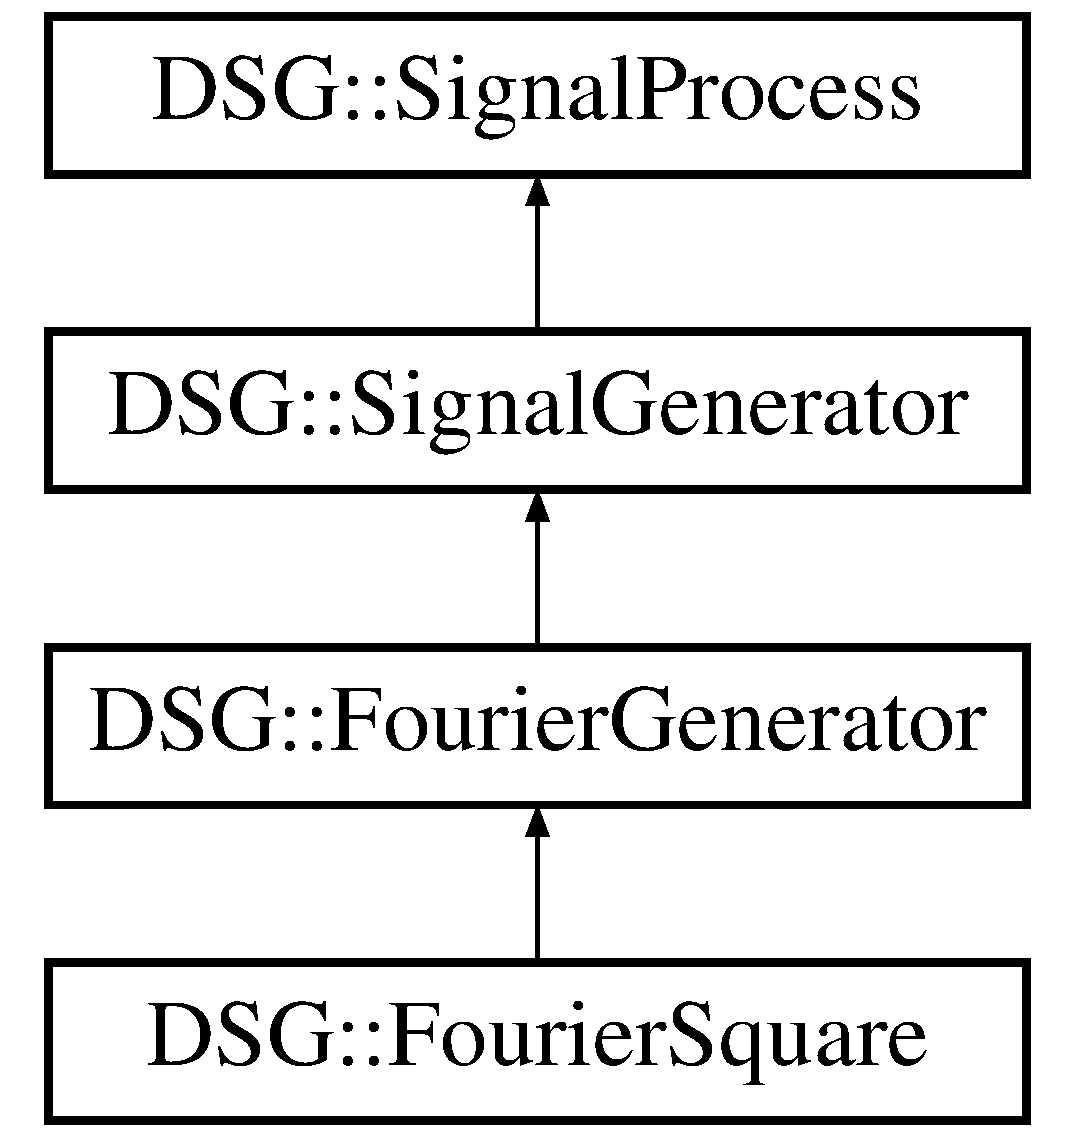
\includegraphics[height=4.000000cm]{classDSG_1_1FourierSquare}
\end{center}
\end{figure}
\subsection*{Public Member Functions}
\begin{DoxyCompactItemize}
\item 
\hyperlink{classDSG_1_1FourierSquare_ac73c7436f0d4b9a9b5d8270d5c8d23ac}{Fourier\+Square} ()
\item 
\hyperlink{classDSG_1_1FourierSquare_ad7cfa0d909e1c7e7d0709e03d0381c3d}{Fourier\+Square} (double const \&frequency, double const \&phase\+\_\+offset)
\item 
virtual \hyperlink{classDSG_1_1FourierSquare_a9a10acb7bddbb26000d806292d78a394}{$\sim$\+Fourier\+Square} ()
\item 
virtual bool \hyperlink{classDSG_1_1FourierSquare_a3e9cfc95b3592eaf04fbcd61a3c68387}{Perform} (\hyperlink{classDSG_1_1Sample}{Sample} \&signal)
\item 
virtual bool \hyperlink{classDSG_1_1FourierSquare_ad9999119d9efc453329ed4b3eaf5f226}{Perform} (\hyperlink{classDSG_1_1RingBuffer}{Ring\+Buffer} \&signal)
\item 
virtual double const \& \hyperlink{classDSG_1_1FourierSquare_a80f94eabad633e105cfa673fdee332d6}{Frequency} (double const \&value)
\item 
virtual double const \& \hyperlink{classDSG_1_1FourierSquare_aa534934e73f4a057005fff6843e3e611}{Frequency} ()
\item 
virtual bool \hyperlink{classDSG_1_1SignalProcess_afdb8220100418893950c1161dd24db67}{Perform} (\hyperlink{classDSG_1_1Sample_aaf2e30d73911eccea99b53eeee15b612}{Sample\+::\+Sample} \&signal)=0
\item 
virtual double const \& \hyperlink{classDSG_1_1SignalGenerator_aedac746c5a70818d120858542ecb7c45}{Frequency} () const 
\item 
virtual double const \& \hyperlink{classDSG_1_1SignalGenerator_a1ce521847edd0b837fd840998f906b4b}{Phase\+Offset} () const 
\item 
virtual double const \& \hyperlink{classDSG_1_1SignalGenerator_a08b71b1f30ba65e629642c570291dc0e}{Phase\+Offset} (double const \&value)
\end{DoxyCompactItemize}
\subsection*{Protected Member Functions}
\begin{DoxyCompactItemize}
\item 
unsigned long \hyperlink{classDSG_1_1FourierGenerator_a6b6e3bbad8ff7443d9ed71f4cdf76739}{\+\_\+max\+Harms} (double \+\_\+frq)
\item 
double \hyperlink{classDSG_1_1SignalGenerator_ac0d781b8673b3a283bf7c133290ede50}{\+\_\+pstep} ()
\item 
double \hyperlink{classDSG_1_1SignalGenerator_ae660eb4caa88b8d278f8d24d0908a487}{\+\_\+pstep\+\_\+rad} ()
\item 
void \hyperlink{classDSG_1_1SignalGenerator_a05baccb38d1e52860d4fcf7cb8430efc}{\+\_\+psync} ()
\end{DoxyCompactItemize}
\subsection*{Protected Attributes}
\begin{DoxyCompactItemize}
\item 
unsigned long \hyperlink{classDSG_1_1FourierSquare_a2b82df6091ad654fe59a44ff6e18a363}{\+\_\+h}
\item 
float \hyperlink{classDSG_1_1FourierSquare_adf625daced0977db90522ba9f4519f91}{\+\_\+a}
\item 
float \hyperlink{classDSG_1_1FourierSquare_a49d0e6f221e67139d47f68c7e4b9b1a9}{phs}
\item 
float \hyperlink{classDSG_1_1FourierSquare_a82bb1d630438aa3ca1d3b1264b8196a5}{stor}
\item 
unsigned short \hyperlink{classDSG_1_1FourierSquare_a4d191ba0c4aad4946cc60f90b7c48d88}{i}
\item 
\hyperlink{classDSG_1_1Sample}{Sample} \hyperlink{classDSG_1_1FourierGenerator_ab96bed1cd59c42e82a689036e5c62bef}{\+\_\+sample}
\item 
\hyperlink{classDSG_1_1Sample}{Sample} \hyperlink{classDSG_1_1FourierGenerator_a6b7f2439b26914cc9df6b6975a2cedac}{\+\_\+storage}
\item 
double \hyperlink{classDSG_1_1SignalGenerator_aa10f6c85d9adee901139ea7fb346f39d}{\+\_\+rate}
\item 
double \hyperlink{classDSG_1_1SignalGenerator_a67e296e3506dcdf09402c667cddff9ac}{\+\_\+frequency}
\item 
double \hyperlink{classDSG_1_1SignalGenerator_ac2271b582bf699275f077ecb642a8cd9}{\+\_\+phasor}
\end{DoxyCompactItemize}
\subsection*{Static Protected Attributes}
\begin{DoxyCompactItemize}
\item 
static \hyperlink{classDSG_1_1HarmonicTable}{D\+S\+G\+::\+Harmonic\+Table} \hyperlink{classDSG_1_1FourierGenerator_a7288408f8e44d5edb5eecc62480243d7}{\+\_\+harmonic\+Table}
\item 
static \hyperlink{classDSG_1_1SineLUT}{D\+S\+G\+::\+Sine\+L\+U\+T}$<$ float, 32768 $>$ \hyperlink{classDSG_1_1FourierGenerator_a1ae5fb243ce05e638bdf0dec8bde7426}{\+\_\+sine\+Lut}
\end{DoxyCompactItemize}


\subsection{Detailed Description}
Fourier Series Based \hyperlink{classDSG_1_1FourierSquare}{Fourier\+Square} Wave. 

Definition at line 15 of file Fourier\+Square.\+h.



\subsection{Constructor \& Destructor Documentation}
\hypertarget{classDSG_1_1FourierSquare_ac73c7436f0d4b9a9b5d8270d5c8d23ac}{\index{D\+S\+G\+::\+Fourier\+Square@{D\+S\+G\+::\+Fourier\+Square}!Fourier\+Square@{Fourier\+Square}}
\index{Fourier\+Square@{Fourier\+Square}!D\+S\+G\+::\+Fourier\+Square@{D\+S\+G\+::\+Fourier\+Square}}
\subsubsection[{Fourier\+Square}]{\setlength{\rightskip}{0pt plus 5cm}D\+S\+G\+::\+Fourier\+Square\+::\+Fourier\+Square (
\begin{DoxyParamCaption}
{}
\end{DoxyParamCaption}
)}}\label{classDSG_1_1FourierSquare_ac73c7436f0d4b9a9b5d8270d5c8d23ac}


Definition at line 9 of file Fourier\+Square.\+cpp.


\begin{DoxyCode}
9                                :\hyperlink{classDSG_1_1FourierGenerator_a43fa07fd160c41fd679a5bd2843a5b0e}{FourierGenerator}(),\hyperlink{classDSG_1_1FourierSquare_adf625daced0977db90522ba9f4519f91}{\_a}((4.0/\hyperlink{PI_8h_a598a3330b3c21701223ee0ca14316eca}{PI})*0.85),
      \hyperlink{classDSG_1_1FourierSquare_a2b82df6091ad654fe59a44ff6e18a363}{\_h}(\hyperlink{classDSG_1_1FourierGenerator_a6b6e3bbad8ff7443d9ed71f4cdf76739}{\_maxHarms}(\hyperlink{classDSG_1_1SignalGenerator_a67e296e3506dcdf09402c667cddff9ac}{\_frequency})+1),\hyperlink{classDSG_1_1FourierSquare_a49d0e6f221e67139d47f68c7e4b9b1a9}{phs}(0),\hyperlink{classDSG_1_1FourierSquare_a82bb1d630438aa3ca1d3b1264b8196a5}{stor}(0)\{
10 \}
\end{DoxyCode}
\hypertarget{classDSG_1_1FourierSquare_ad7cfa0d909e1c7e7d0709e03d0381c3d}{\index{D\+S\+G\+::\+Fourier\+Square@{D\+S\+G\+::\+Fourier\+Square}!Fourier\+Square@{Fourier\+Square}}
\index{Fourier\+Square@{Fourier\+Square}!D\+S\+G\+::\+Fourier\+Square@{D\+S\+G\+::\+Fourier\+Square}}
\subsubsection[{Fourier\+Square}]{\setlength{\rightskip}{0pt plus 5cm}D\+S\+G\+::\+Fourier\+Square\+::\+Fourier\+Square (
\begin{DoxyParamCaption}
\item[{double const \&}]{frequency, }
\item[{double const \&}]{phase\+\_\+offset}
\end{DoxyParamCaption}
)}}\label{classDSG_1_1FourierSquare_ad7cfa0d909e1c7e7d0709e03d0381c3d}


Definition at line 11 of file Fourier\+Square.\+cpp.


\begin{DoxyCode}
11                                                                                  :
      \hyperlink{classDSG_1_1FourierGenerator_a43fa07fd160c41fd679a5bd2843a5b0e}{FourierGenerator}(frequency,phase\_offset),\hyperlink{classDSG_1_1FourierSquare_adf625daced0977db90522ba9f4519f91}{\_a}((4.0/\hyperlink{PI_8h_a598a3330b3c21701223ee0ca14316eca}{PI})*0.85),
      \hyperlink{classDSG_1_1FourierSquare_a2b82df6091ad654fe59a44ff6e18a363}{\_h}(\hyperlink{classDSG_1_1FourierGenerator_a6b6e3bbad8ff7443d9ed71f4cdf76739}{\_maxHarms}(\hyperlink{classDSG_1_1SignalGenerator_a67e296e3506dcdf09402c667cddff9ac}{\_frequency})+1),\hyperlink{classDSG_1_1FourierSquare_a49d0e6f221e67139d47f68c7e4b9b1a9}{phs}(0),\hyperlink{classDSG_1_1FourierSquare_a82bb1d630438aa3ca1d3b1264b8196a5}{stor}(0)\{
12     \hyperlink{classDSG_1_1FourierGenerator_ab96bed1cd59c42e82a689036e5c62bef}{\_sample}=0;
13     \hyperlink{classDSG_1_1FourierGenerator_a6b7f2439b26914cc9df6b6975a2cedac}{\_storage}=0;
14 \}
\end{DoxyCode}
\hypertarget{classDSG_1_1FourierSquare_a9a10acb7bddbb26000d806292d78a394}{\index{D\+S\+G\+::\+Fourier\+Square@{D\+S\+G\+::\+Fourier\+Square}!````~Fourier\+Square@{$\sim$\+Fourier\+Square}}
\index{````~Fourier\+Square@{$\sim$\+Fourier\+Square}!D\+S\+G\+::\+Fourier\+Square@{D\+S\+G\+::\+Fourier\+Square}}
\subsubsection[{$\sim$\+Fourier\+Square}]{\setlength{\rightskip}{0pt plus 5cm}D\+S\+G\+::\+Fourier\+Square\+::$\sim$\+Fourier\+Square (
\begin{DoxyParamCaption}
{}
\end{DoxyParamCaption}
)\hspace{0.3cm}{\ttfamily [virtual]}}}\label{classDSG_1_1FourierSquare_a9a10acb7bddbb26000d806292d78a394}


Definition at line 15 of file Fourier\+Square.\+cpp.


\begin{DoxyCode}
15 \{\}
\end{DoxyCode}


\subsection{Member Function Documentation}
\hypertarget{classDSG_1_1FourierGenerator_a6b6e3bbad8ff7443d9ed71f4cdf76739}{\index{D\+S\+G\+::\+Fourier\+Square@{D\+S\+G\+::\+Fourier\+Square}!\+\_\+max\+Harms@{\+\_\+max\+Harms}}
\index{\+\_\+max\+Harms@{\+\_\+max\+Harms}!D\+S\+G\+::\+Fourier\+Square@{D\+S\+G\+::\+Fourier\+Square}}
\subsubsection[{\+\_\+max\+Harms}]{\setlength{\rightskip}{0pt plus 5cm}unsigned long D\+S\+G\+::\+Fourier\+Generator\+::\+\_\+max\+Harms (
\begin{DoxyParamCaption}
\item[{double}]{\+\_\+frq}
\end{DoxyParamCaption}
)\hspace{0.3cm}{\ttfamily [inline]}, {\ttfamily [protected]}, {\ttfamily [inherited]}}}\label{classDSG_1_1FourierGenerator_a6b6e3bbad8ff7443d9ed71f4cdf76739}


Definition at line 45 of file Fourier\+Generator.\+h.


\begin{DoxyCode}
45                                                                    \{
46             \textcolor{comment}{//double softLim = 0.45;}
47             \textcolor{comment}{//double hardLim = 0.5;}
48             
49             \textcolor{keywordtype}{double} \_s =  \hyperlink{namespaceDSG_a0c5c3a251b3688398da18138c5efe4bf}{Sample\_Rate}()* (20000.0/ \hyperlink{namespaceDSG_a0c5c3a251b3688398da18138c5efe4bf}{Sample\_Rate}());\textcolor{comment}{//uses harmonic roll
       of based on max human hearing and sample rate}
50             \_s/=\_frq;
51             \textcolor{keywordflow}{return} trunc(\_s);
52         \}
\end{DoxyCode}
\hypertarget{classDSG_1_1SignalGenerator_ac0d781b8673b3a283bf7c133290ede50}{\index{D\+S\+G\+::\+Fourier\+Square@{D\+S\+G\+::\+Fourier\+Square}!\+\_\+pstep@{\+\_\+pstep}}
\index{\+\_\+pstep@{\+\_\+pstep}!D\+S\+G\+::\+Fourier\+Square@{D\+S\+G\+::\+Fourier\+Square}}
\subsubsection[{\+\_\+pstep}]{\setlength{\rightskip}{0pt plus 5cm}double D\+S\+G\+::\+Signal\+Generator\+::\+\_\+pstep (
\begin{DoxyParamCaption}
{}
\end{DoxyParamCaption}
)\hspace{0.3cm}{\ttfamily [inline]}, {\ttfamily [protected]}, {\ttfamily [inherited]}}}\label{classDSG_1_1SignalGenerator_ac0d781b8673b3a283bf7c133290ede50}


Definition at line 52 of file Signal\+Generator.\+h.


\begin{DoxyCode}
52                                          \{
53         value = \hyperlink{classDSG_1_1SignalGenerator_ac2271b582bf699275f077ecb642a8cd9}{\_phasor};
54         \hyperlink{classDSG_1_1SignalGenerator_ac2271b582bf699275f077ecb642a8cd9}{\_phasor}+=\hyperlink{classDSG_1_1SignalGenerator_aa10f6c85d9adee901139ea7fb346f39d}{\_rate};
55         \hyperlink{classDSG_1_1SignalGenerator_ac2271b582bf699275f077ecb642a8cd9}{\_phasor}>1?\hyperlink{classDSG_1_1SignalGenerator_ac2271b582bf699275f077ecb642a8cd9}{\_phasor}-=1:0;\textcolor{comment}{//cheaper cheaper %1}
56         \textcolor{comment}{//\_phasor -= (unsigned long)\_phasor;//cheaper %1}
57         \textcolor{keywordflow}{return} value;
58     \}
\end{DoxyCode}
\hypertarget{classDSG_1_1SignalGenerator_ae660eb4caa88b8d278f8d24d0908a487}{\index{D\+S\+G\+::\+Fourier\+Square@{D\+S\+G\+::\+Fourier\+Square}!\+\_\+pstep\+\_\+rad@{\+\_\+pstep\+\_\+rad}}
\index{\+\_\+pstep\+\_\+rad@{\+\_\+pstep\+\_\+rad}!D\+S\+G\+::\+Fourier\+Square@{D\+S\+G\+::\+Fourier\+Square}}
\subsubsection[{\+\_\+pstep\+\_\+rad}]{\setlength{\rightskip}{0pt plus 5cm}double D\+S\+G\+::\+Signal\+Generator\+::\+\_\+pstep\+\_\+rad (
\begin{DoxyParamCaption}
{}
\end{DoxyParamCaption}
)\hspace{0.3cm}{\ttfamily [inline]}, {\ttfamily [protected]}, {\ttfamily [inherited]}}}\label{classDSG_1_1SignalGenerator_ae660eb4caa88b8d278f8d24d0908a487}


Definition at line 59 of file Signal\+Generator.\+h.


\begin{DoxyCode}
59                                              \{
60         \textcolor{keywordflow}{return} \hyperlink{PI_8h_a4912c64aec0c943b7985db6cb61ff83a}{TWOPI} * \hyperlink{classDSG_1_1SignalGenerator_ac0d781b8673b3a283bf7c133290ede50}{\_pstep}();
61     \}
\end{DoxyCode}
\hypertarget{classDSG_1_1SignalGenerator_a05baccb38d1e52860d4fcf7cb8430efc}{\index{D\+S\+G\+::\+Fourier\+Square@{D\+S\+G\+::\+Fourier\+Square}!\+\_\+psync@{\+\_\+psync}}
\index{\+\_\+psync@{\+\_\+psync}!D\+S\+G\+::\+Fourier\+Square@{D\+S\+G\+::\+Fourier\+Square}}
\subsubsection[{\+\_\+psync}]{\setlength{\rightskip}{0pt plus 5cm}void D\+S\+G\+::\+Signal\+Generator\+::\+\_\+psync (
\begin{DoxyParamCaption}
{}
\end{DoxyParamCaption}
)\hspace{0.3cm}{\ttfamily [inline]}, {\ttfamily [protected]}, {\ttfamily [inherited]}}}\label{classDSG_1_1SignalGenerator_a05baccb38d1e52860d4fcf7cb8430efc}


Definition at line 62 of file Signal\+Generator.\+h.


\begin{DoxyCode}
62                                        \{
63         \hyperlink{classDSG_1_1SignalGenerator_ac2271b582bf699275f077ecb642a8cd9}{\_phasor} = \_phase\_offset;
64     \}
\end{DoxyCode}
\hypertarget{classDSG_1_1FourierSquare_a80f94eabad633e105cfa673fdee332d6}{\index{D\+S\+G\+::\+Fourier\+Square@{D\+S\+G\+::\+Fourier\+Square}!Frequency@{Frequency}}
\index{Frequency@{Frequency}!D\+S\+G\+::\+Fourier\+Square@{D\+S\+G\+::\+Fourier\+Square}}
\subsubsection[{Frequency}]{\setlength{\rightskip}{0pt plus 5cm}double const \& D\+S\+G\+::\+Fourier\+Square\+::\+Frequency (
\begin{DoxyParamCaption}
\item[{double const \&}]{value}
\end{DoxyParamCaption}
)\hspace{0.3cm}{\ttfamily [virtual]}}}\label{classDSG_1_1FourierSquare_a80f94eabad633e105cfa673fdee332d6}


Reimplemented from \hyperlink{classDSG_1_1SignalGenerator_ae3ce8d45bafabbd86a0f535b15c3cd46}{D\+S\+G\+::\+Signal\+Generator}.



Definition at line 16 of file Fourier\+Square.\+cpp.


\begin{DoxyCode}
16                                                             \{
17     \hyperlink{classDSG_1_1SignalGenerator_a67e296e3506dcdf09402c667cddff9ac}{\_frequency} = value;
18     \hyperlink{classDSG_1_1SignalGenerator_aa10f6c85d9adee901139ea7fb346f39d}{\_rate} = \hyperlink{classDSG_1_1SignalGenerator_a67e296e3506dcdf09402c667cddff9ac}{\_frequency}/ \hyperlink{namespaceDSG_a0c5c3a251b3688398da18138c5efe4bf}{Sample\_Rate}();
19     \hyperlink{classDSG_1_1FourierSquare_a2b82df6091ad654fe59a44ff6e18a363}{\_h} = \hyperlink{classDSG_1_1FourierGenerator_a6b6e3bbad8ff7443d9ed71f4cdf76739}{\_maxHarms}(\hyperlink{classDSG_1_1SignalGenerator_a67e296e3506dcdf09402c667cddff9ac}{\_frequency})+1;
20     \textcolor{keywordflow}{return} \hyperlink{classDSG_1_1SignalGenerator_a67e296e3506dcdf09402c667cddff9ac}{\_frequency};
21 \}
\end{DoxyCode}
\hypertarget{classDSG_1_1SignalGenerator_aedac746c5a70818d120858542ecb7c45}{\index{D\+S\+G\+::\+Fourier\+Square@{D\+S\+G\+::\+Fourier\+Square}!Frequency@{Frequency}}
\index{Frequency@{Frequency}!D\+S\+G\+::\+Fourier\+Square@{D\+S\+G\+::\+Fourier\+Square}}
\subsubsection[{Frequency}]{\setlength{\rightskip}{0pt plus 5cm}double const \& D\+S\+G\+::\+Signal\+Generator\+::\+Frequency (
\begin{DoxyParamCaption}
{}
\end{DoxyParamCaption}
) const\hspace{0.3cm}{\ttfamily [virtual]}, {\ttfamily [inherited]}}}\label{classDSG_1_1SignalGenerator_aedac746c5a70818d120858542ecb7c45}


Definition at line 14 of file Signal\+Generator.\+cpp.


\begin{DoxyCode}
14                                                 \{
15     \textcolor{keywordflow}{return} \hyperlink{classDSG_1_1SignalGenerator_a67e296e3506dcdf09402c667cddff9ac}{\_frequency};
16 \}
\end{DoxyCode}
\hypertarget{classDSG_1_1FourierSquare_aa534934e73f4a057005fff6843e3e611}{\index{D\+S\+G\+::\+Fourier\+Square@{D\+S\+G\+::\+Fourier\+Square}!Frequency@{Frequency}}
\index{Frequency@{Frequency}!D\+S\+G\+::\+Fourier\+Square@{D\+S\+G\+::\+Fourier\+Square}}
\subsubsection[{Frequency}]{\setlength{\rightskip}{0pt plus 5cm}double const \& D\+S\+G\+::\+Fourier\+Square\+::\+Frequency (
\begin{DoxyParamCaption}
{}
\end{DoxyParamCaption}
)\hspace{0.3cm}{\ttfamily [virtual]}}}\label{classDSG_1_1FourierSquare_aa534934e73f4a057005fff6843e3e611}


Definition at line 22 of file Fourier\+Square.\+cpp.


\begin{DoxyCode}
22                                          \{
23     \textcolor{keywordflow}{return} this->\hyperlink{classDSG_1_1SignalGenerator_a67e296e3506dcdf09402c667cddff9ac}{\_frequency};
24 \}\end{DoxyCode}
\hypertarget{classDSG_1_1FourierSquare_a3e9cfc95b3592eaf04fbcd61a3c68387}{\index{D\+S\+G\+::\+Fourier\+Square@{D\+S\+G\+::\+Fourier\+Square}!Perform@{Perform}}
\index{Perform@{Perform}!D\+S\+G\+::\+Fourier\+Square@{D\+S\+G\+::\+Fourier\+Square}}
\subsubsection[{Perform}]{\setlength{\rightskip}{0pt plus 5cm}bool D\+S\+G\+::\+Fourier\+Square\+::\+Perform (
\begin{DoxyParamCaption}
\item[{{\bf Sample} \&}]{signal}
\end{DoxyParamCaption}
)\hspace{0.3cm}{\ttfamily [inline]}, {\ttfamily [virtual]}}}\label{classDSG_1_1FourierSquare_a3e9cfc95b3592eaf04fbcd61a3c68387}


Reimplemented from \hyperlink{classDSG_1_1FourierGenerator_a7f5e34e65c1fe757318fb5b063dabde9}{D\+S\+G\+::\+Fourier\+Generator}.



Definition at line 31 of file Fourier\+Square.\+h.


\begin{DoxyCode}
31                                                      \{
32         \hyperlink{classDSG_1_1FourierSquare_a49d0e6f221e67139d47f68c7e4b9b1a9}{phs} = \hyperlink{classDSG_1_1SignalGenerator_ac0d781b8673b3a283bf7c133290ede50}{\_pstep}();
33         
34         \hyperlink{classDSG_1_1FourierSquare_a82bb1d630438aa3ca1d3b1264b8196a5}{stor}=0;
35         \textcolor{keywordflow}{for} (\hyperlink{classDSG_1_1FourierSquare_a4d191ba0c4aad4946cc60f90b7c48d88}{i}=1; \hyperlink{classDSG_1_1FourierSquare_a4d191ba0c4aad4946cc60f90b7c48d88}{i}<\hyperlink{classDSG_1_1FourierSquare_a2b82df6091ad654fe59a44ff6e18a363}{\_h}; \hyperlink{classDSG_1_1FourierSquare_a4d191ba0c4aad4946cc60f90b7c48d88}{i}+=2) \{
36             \hyperlink{classDSG_1_1FourierSquare_a82bb1d630438aa3ca1d3b1264b8196a5}{stor} += \hyperlink{classDSG_1_1FourierGenerator_a7288408f8e44d5edb5eecc62480243d7}{\_harmonicTable}.\hyperlink{classDSG_1_1HarmonicTable_a979840fc73c8c4b6a7c24eaa3ba6387b}{Saw}(\hyperlink{classDSG_1_1FourierSquare_a4d191ba0c4aad4946cc60f90b7c48d88}{i}) * \hyperlink{classDSG_1_1FourierGenerator_a1ae5fb243ce05e638bdf0dec8bde7426}{\_sineLut}(
      \hyperlink{classDSG_1_1FourierSquare_a49d0e6f221e67139d47f68c7e4b9b1a9}{phs}*\hyperlink{classDSG_1_1FourierSquare_a4d191ba0c4aad4946cc60f90b7c48d88}{i});
37         \}
38         \hyperlink{classDSG_1_1FourierSquare_a82bb1d630438aa3ca1d3b1264b8196a5}{stor} *= \hyperlink{classDSG_1_1FourierSquare_adf625daced0977db90522ba9f4519f91}{\_a};
39         signal = \hyperlink{classDSG_1_1FourierSquare_a82bb1d630438aa3ca1d3b1264b8196a5}{stor};
40         \textcolor{keywordflow}{return} \textcolor{keyword}{true};
41     \}
\end{DoxyCode}
\hypertarget{classDSG_1_1SignalProcess_afdb8220100418893950c1161dd24db67}{\index{D\+S\+G\+::\+Fourier\+Square@{D\+S\+G\+::\+Fourier\+Square}!Perform@{Perform}}
\index{Perform@{Perform}!D\+S\+G\+::\+Fourier\+Square@{D\+S\+G\+::\+Fourier\+Square}}
\subsubsection[{Perform}]{\setlength{\rightskip}{0pt plus 5cm}virtual bool D\+S\+G\+::\+Signal\+Process\+::\+Perform (
\begin{DoxyParamCaption}
\item[{{\bf Sample\+::\+Sample} \&}]{signal}
\end{DoxyParamCaption}
)\hspace{0.3cm}{\ttfamily [inline]}, {\ttfamily [pure virtual]}, {\ttfamily [inherited]}}}\label{classDSG_1_1SignalProcess_afdb8220100418893950c1161dd24db67}
\hypertarget{classDSG_1_1FourierSquare_ad9999119d9efc453329ed4b3eaf5f226}{\index{D\+S\+G\+::\+Fourier\+Square@{D\+S\+G\+::\+Fourier\+Square}!Perform@{Perform}}
\index{Perform@{Perform}!D\+S\+G\+::\+Fourier\+Square@{D\+S\+G\+::\+Fourier\+Square}}
\subsubsection[{Perform}]{\setlength{\rightskip}{0pt plus 5cm}bool D\+S\+G\+::\+Fourier\+Square\+::\+Perform (
\begin{DoxyParamCaption}
\item[{{\bf Ring\+Buffer} \&}]{signal}
\end{DoxyParamCaption}
)\hspace{0.3cm}{\ttfamily [inline]}, {\ttfamily [virtual]}}}\label{classDSG_1_1FourierSquare_ad9999119d9efc453329ed4b3eaf5f226}


Reimplemented from \hyperlink{classDSG_1_1FourierGenerator_a8b2aca91155dbb524aaf13867f273188}{D\+S\+G\+::\+Fourier\+Generator}.



Definition at line 42 of file Fourier\+Square.\+h.


\begin{DoxyCode}
42                                                          \{
43         signal.Flush();
44         \textcolor{keywordflow}{while} (!signal.Full()) \{
45             \textcolor{keywordflow}{if} (\hyperlink{classDSG_1_1FourierSquare_a3e9cfc95b3592eaf04fbcd61a3c68387}{Perform}(\hyperlink{classDSG_1_1FourierGenerator_ab96bed1cd59c42e82a689036e5c62bef}{\_sample})) \{
46                 \textcolor{keywordflow}{if}(signal.Write(\hyperlink{classDSG_1_1FourierGenerator_ab96bed1cd59c42e82a689036e5c62bef}{\_sample}))\{
47                 \}\textcolor{keywordflow}{else} \textcolor{keywordflow}{return} \textcolor{keyword}{false};
48             \}\textcolor{keywordflow}{else} \textcolor{keywordflow}{return} \textcolor{keyword}{false};
49         \}\textcolor{keywordflow}{return} \textcolor{keyword}{true};
50     \}
\end{DoxyCode}
\hypertarget{classDSG_1_1SignalGenerator_a1ce521847edd0b837fd840998f906b4b}{\index{D\+S\+G\+::\+Fourier\+Square@{D\+S\+G\+::\+Fourier\+Square}!Phase\+Offset@{Phase\+Offset}}
\index{Phase\+Offset@{Phase\+Offset}!D\+S\+G\+::\+Fourier\+Square@{D\+S\+G\+::\+Fourier\+Square}}
\subsubsection[{Phase\+Offset}]{\setlength{\rightskip}{0pt plus 5cm}double const \& D\+S\+G\+::\+Signal\+Generator\+::\+Phase\+Offset (
\begin{DoxyParamCaption}
{}
\end{DoxyParamCaption}
) const\hspace{0.3cm}{\ttfamily [virtual]}, {\ttfamily [inherited]}}}\label{classDSG_1_1SignalGenerator_a1ce521847edd0b837fd840998f906b4b}


Definition at line 22 of file Signal\+Generator.\+cpp.


\begin{DoxyCode}
22                                                   \{
23     \textcolor{keywordflow}{return} \_phase\_offset;
24 \}
\end{DoxyCode}
\hypertarget{classDSG_1_1SignalGenerator_a08b71b1f30ba65e629642c570291dc0e}{\index{D\+S\+G\+::\+Fourier\+Square@{D\+S\+G\+::\+Fourier\+Square}!Phase\+Offset@{Phase\+Offset}}
\index{Phase\+Offset@{Phase\+Offset}!D\+S\+G\+::\+Fourier\+Square@{D\+S\+G\+::\+Fourier\+Square}}
\subsubsection[{Phase\+Offset}]{\setlength{\rightskip}{0pt plus 5cm}double const \& D\+S\+G\+::\+Signal\+Generator\+::\+Phase\+Offset (
\begin{DoxyParamCaption}
\item[{double const \&}]{value}
\end{DoxyParamCaption}
)\hspace{0.3cm}{\ttfamily [virtual]}, {\ttfamily [inherited]}}}\label{classDSG_1_1SignalGenerator_a08b71b1f30ba65e629642c570291dc0e}


Definition at line 25 of file Signal\+Generator.\+cpp.


\begin{DoxyCode}
25                                                                 \{
26     \_phase\_offset-=value;
27     \hyperlink{classDSG_1_1SignalGenerator_ac2271b582bf699275f077ecb642a8cd9}{\_phasor}-=\_phase\_offset;
28     \_phase\_offset=value;
29     \textcolor{keywordflow}{return} \_phase\_offset;
30 \}\end{DoxyCode}


\subsection{Member Data Documentation}
\hypertarget{classDSG_1_1FourierSquare_adf625daced0977db90522ba9f4519f91}{\index{D\+S\+G\+::\+Fourier\+Square@{D\+S\+G\+::\+Fourier\+Square}!\+\_\+a@{\+\_\+a}}
\index{\+\_\+a@{\+\_\+a}!D\+S\+G\+::\+Fourier\+Square@{D\+S\+G\+::\+Fourier\+Square}}
\subsubsection[{\+\_\+a}]{\setlength{\rightskip}{0pt plus 5cm}float D\+S\+G\+::\+Fourier\+Square\+::\+\_\+a\hspace{0.3cm}{\ttfamily [protected]}}}\label{classDSG_1_1FourierSquare_adf625daced0977db90522ba9f4519f91}


Definition at line 26 of file Fourier\+Square.\+h.

\hypertarget{classDSG_1_1SignalGenerator_a67e296e3506dcdf09402c667cddff9ac}{\index{D\+S\+G\+::\+Fourier\+Square@{D\+S\+G\+::\+Fourier\+Square}!\+\_\+frequency@{\+\_\+frequency}}
\index{\+\_\+frequency@{\+\_\+frequency}!D\+S\+G\+::\+Fourier\+Square@{D\+S\+G\+::\+Fourier\+Square}}
\subsubsection[{\+\_\+frequency}]{\setlength{\rightskip}{0pt plus 5cm}double D\+S\+G\+::\+Signal\+Generator\+::\+\_\+frequency\hspace{0.3cm}{\ttfamily [protected]}, {\ttfamily [inherited]}}}\label{classDSG_1_1SignalGenerator_a67e296e3506dcdf09402c667cddff9ac}


Definition at line 28 of file Signal\+Generator.\+h.

\hypertarget{classDSG_1_1FourierSquare_a2b82df6091ad654fe59a44ff6e18a363}{\index{D\+S\+G\+::\+Fourier\+Square@{D\+S\+G\+::\+Fourier\+Square}!\+\_\+h@{\+\_\+h}}
\index{\+\_\+h@{\+\_\+h}!D\+S\+G\+::\+Fourier\+Square@{D\+S\+G\+::\+Fourier\+Square}}
\subsubsection[{\+\_\+h}]{\setlength{\rightskip}{0pt plus 5cm}unsigned long D\+S\+G\+::\+Fourier\+Square\+::\+\_\+h\hspace{0.3cm}{\ttfamily [protected]}}}\label{classDSG_1_1FourierSquare_a2b82df6091ad654fe59a44ff6e18a363}


Definition at line 25 of file Fourier\+Square.\+h.

\hypertarget{classDSG_1_1FourierGenerator_a7288408f8e44d5edb5eecc62480243d7}{\index{D\+S\+G\+::\+Fourier\+Square@{D\+S\+G\+::\+Fourier\+Square}!\+\_\+harmonic\+Table@{\+\_\+harmonic\+Table}}
\index{\+\_\+harmonic\+Table@{\+\_\+harmonic\+Table}!D\+S\+G\+::\+Fourier\+Square@{D\+S\+G\+::\+Fourier\+Square}}
\subsubsection[{\+\_\+harmonic\+Table}]{\setlength{\rightskip}{0pt plus 5cm}{\bf D\+S\+G\+::\+Harmonic\+Table} D\+S\+G\+::\+Fourier\+Generator\+::\+\_\+harmonic\+Table\hspace{0.3cm}{\ttfamily [static]}, {\ttfamily [protected]}, {\ttfamily [inherited]}}}\label{classDSG_1_1FourierGenerator_a7288408f8e44d5edb5eecc62480243d7}


Definition at line 34 of file Fourier\+Generator.\+h.

\hypertarget{classDSG_1_1SignalGenerator_ac2271b582bf699275f077ecb642a8cd9}{\index{D\+S\+G\+::\+Fourier\+Square@{D\+S\+G\+::\+Fourier\+Square}!\+\_\+phasor@{\+\_\+phasor}}
\index{\+\_\+phasor@{\+\_\+phasor}!D\+S\+G\+::\+Fourier\+Square@{D\+S\+G\+::\+Fourier\+Square}}
\subsubsection[{\+\_\+phasor}]{\setlength{\rightskip}{0pt plus 5cm}double D\+S\+G\+::\+Signal\+Generator\+::\+\_\+phasor\hspace{0.3cm}{\ttfamily [protected]}, {\ttfamily [inherited]}}}\label{classDSG_1_1SignalGenerator_ac2271b582bf699275f077ecb642a8cd9}


Definition at line 38 of file Signal\+Generator.\+h.

\hypertarget{classDSG_1_1SignalGenerator_aa10f6c85d9adee901139ea7fb346f39d}{\index{D\+S\+G\+::\+Fourier\+Square@{D\+S\+G\+::\+Fourier\+Square}!\+\_\+rate@{\+\_\+rate}}
\index{\+\_\+rate@{\+\_\+rate}!D\+S\+G\+::\+Fourier\+Square@{D\+S\+G\+::\+Fourier\+Square}}
\subsubsection[{\+\_\+rate}]{\setlength{\rightskip}{0pt plus 5cm}double D\+S\+G\+::\+Signal\+Generator\+::\+\_\+rate\hspace{0.3cm}{\ttfamily [protected]}, {\ttfamily [inherited]}}}\label{classDSG_1_1SignalGenerator_aa10f6c85d9adee901139ea7fb346f39d}


Definition at line 27 of file Signal\+Generator.\+h.

\hypertarget{classDSG_1_1FourierGenerator_ab96bed1cd59c42e82a689036e5c62bef}{\index{D\+S\+G\+::\+Fourier\+Square@{D\+S\+G\+::\+Fourier\+Square}!\+\_\+sample@{\+\_\+sample}}
\index{\+\_\+sample@{\+\_\+sample}!D\+S\+G\+::\+Fourier\+Square@{D\+S\+G\+::\+Fourier\+Square}}
\subsubsection[{\+\_\+sample}]{\setlength{\rightskip}{0pt plus 5cm}{\bf Sample} D\+S\+G\+::\+Fourier\+Generator\+::\+\_\+sample\hspace{0.3cm}{\ttfamily [protected]}, {\ttfamily [inherited]}}}\label{classDSG_1_1FourierGenerator_ab96bed1cd59c42e82a689036e5c62bef}


Definition at line 32 of file Fourier\+Generator.\+h.

\hypertarget{classDSG_1_1FourierGenerator_a1ae5fb243ce05e638bdf0dec8bde7426}{\index{D\+S\+G\+::\+Fourier\+Square@{D\+S\+G\+::\+Fourier\+Square}!\+\_\+sine\+Lut@{\+\_\+sine\+Lut}}
\index{\+\_\+sine\+Lut@{\+\_\+sine\+Lut}!D\+S\+G\+::\+Fourier\+Square@{D\+S\+G\+::\+Fourier\+Square}}
\subsubsection[{\+\_\+sine\+Lut}]{\setlength{\rightskip}{0pt plus 5cm}{\bf D\+S\+G\+::\+Sine\+L\+U\+T}$<$ float, 32768 $>$ D\+S\+G\+::\+Fourier\+Generator\+::\+\_\+sine\+Lut\hspace{0.3cm}{\ttfamily [static]}, {\ttfamily [protected]}, {\ttfamily [inherited]}}}\label{classDSG_1_1FourierGenerator_a1ae5fb243ce05e638bdf0dec8bde7426}


Definition at line 35 of file Fourier\+Generator.\+h.

\hypertarget{classDSG_1_1FourierGenerator_a6b7f2439b26914cc9df6b6975a2cedac}{\index{D\+S\+G\+::\+Fourier\+Square@{D\+S\+G\+::\+Fourier\+Square}!\+\_\+storage@{\+\_\+storage}}
\index{\+\_\+storage@{\+\_\+storage}!D\+S\+G\+::\+Fourier\+Square@{D\+S\+G\+::\+Fourier\+Square}}
\subsubsection[{\+\_\+storage}]{\setlength{\rightskip}{0pt plus 5cm}{\bf Sample} D\+S\+G\+::\+Fourier\+Generator\+::\+\_\+storage\hspace{0.3cm}{\ttfamily [protected]}, {\ttfamily [inherited]}}}\label{classDSG_1_1FourierGenerator_a6b7f2439b26914cc9df6b6975a2cedac}


Definition at line 33 of file Fourier\+Generator.\+h.

\hypertarget{classDSG_1_1FourierSquare_a4d191ba0c4aad4946cc60f90b7c48d88}{\index{D\+S\+G\+::\+Fourier\+Square@{D\+S\+G\+::\+Fourier\+Square}!i@{i}}
\index{i@{i}!D\+S\+G\+::\+Fourier\+Square@{D\+S\+G\+::\+Fourier\+Square}}
\subsubsection[{i}]{\setlength{\rightskip}{0pt plus 5cm}unsigned short D\+S\+G\+::\+Fourier\+Square\+::i\hspace{0.3cm}{\ttfamily [protected]}}}\label{classDSG_1_1FourierSquare_a4d191ba0c4aad4946cc60f90b7c48d88}


Definition at line 29 of file Fourier\+Square.\+h.

\hypertarget{classDSG_1_1FourierSquare_a49d0e6f221e67139d47f68c7e4b9b1a9}{\index{D\+S\+G\+::\+Fourier\+Square@{D\+S\+G\+::\+Fourier\+Square}!phs@{phs}}
\index{phs@{phs}!D\+S\+G\+::\+Fourier\+Square@{D\+S\+G\+::\+Fourier\+Square}}
\subsubsection[{phs}]{\setlength{\rightskip}{0pt plus 5cm}float D\+S\+G\+::\+Fourier\+Square\+::phs\hspace{0.3cm}{\ttfamily [protected]}}}\label{classDSG_1_1FourierSquare_a49d0e6f221e67139d47f68c7e4b9b1a9}


Definition at line 27 of file Fourier\+Square.\+h.

\hypertarget{classDSG_1_1FourierSquare_a82bb1d630438aa3ca1d3b1264b8196a5}{\index{D\+S\+G\+::\+Fourier\+Square@{D\+S\+G\+::\+Fourier\+Square}!stor@{stor}}
\index{stor@{stor}!D\+S\+G\+::\+Fourier\+Square@{D\+S\+G\+::\+Fourier\+Square}}
\subsubsection[{stor}]{\setlength{\rightskip}{0pt plus 5cm}float D\+S\+G\+::\+Fourier\+Square\+::stor\hspace{0.3cm}{\ttfamily [protected]}}}\label{classDSG_1_1FourierSquare_a82bb1d630438aa3ca1d3b1264b8196a5}


Definition at line 28 of file Fourier\+Square.\+h.



The documentation for this class was generated from the following files\+:\begin{DoxyCompactItemize}
\item 
/\+Users/alexanderzywicki/\+Documents/\+School\+\_\+\+Stuff/\+Fall\+\_\+2014/\+Digital\+\_\+\+Signal\+\_\+\+Generation\+\_\+and\+\_\+\+Analysis/src/include/\hyperlink{FourierSquare_8h}{Fourier\+Square.\+h}\item 
/\+Users/alexanderzywicki/\+Documents/\+School\+\_\+\+Stuff/\+Fall\+\_\+2014/\+Digital\+\_\+\+Signal\+\_\+\+Generation\+\_\+and\+\_\+\+Analysis/src/\hyperlink{FourierSquare_8cpp}{Fourier\+Square.\+cpp}\end{DoxyCompactItemize}

\hypertarget{classDSG_1_1FourierTriangle}{\section{D\+S\+G\+:\+:Fourier\+Triangle Class Reference}
\label{classDSG_1_1FourierTriangle}\index{D\+S\+G\+::\+Fourier\+Triangle@{D\+S\+G\+::\+Fourier\+Triangle}}
}


Fourier Series Based \hyperlink{classDSG_1_1FourierTriangle}{Fourier\+Triangle} Wave.  




{\ttfamily \#include $<$Fourier\+Triangle.\+h$>$}

Inheritance diagram for D\+S\+G\+:\+:Fourier\+Triangle\+:\begin{figure}[H]
\begin{center}
\leavevmode
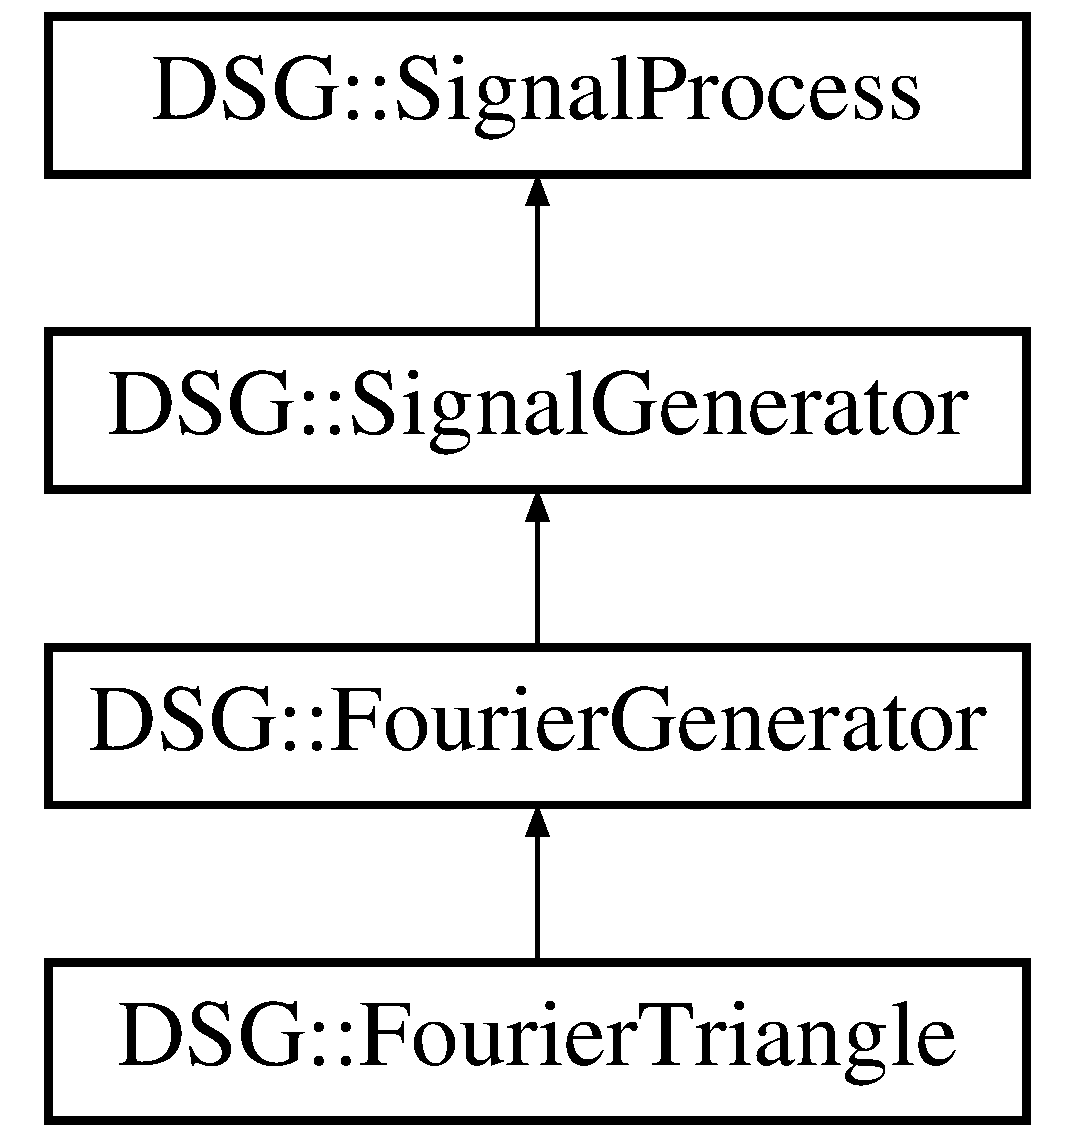
\includegraphics[height=4.000000cm]{classDSG_1_1FourierTriangle}
\end{center}
\end{figure}
\subsection*{Public Member Functions}
\begin{DoxyCompactItemize}
\item 
\hyperlink{classDSG_1_1FourierTriangle_a5274aa0468d5e566f5a23d517b0e0767}{Fourier\+Triangle} ()
\item 
\hyperlink{classDSG_1_1FourierTriangle_a1d23bd3033e60968f2cd17610c424b86}{Fourier\+Triangle} (double const \&frequency, double const \&phase\+\_\+offset)
\item 
virtual \hyperlink{classDSG_1_1FourierTriangle_a9844e13eed3b8b5583d81a14d2e4c87b}{$\sim$\+Fourier\+Triangle} ()
\item 
virtual bool \hyperlink{classDSG_1_1FourierTriangle_ae927efb96f8d40f620dd02bdaaeef4d5}{Perform} (\hyperlink{classDSG_1_1Sample}{Sample} \&signal)
\item 
virtual bool \hyperlink{classDSG_1_1FourierTriangle_a017e2b59123ff3afa9a5c0e833e5f482}{Perform} (\hyperlink{classDSG_1_1RingBuffer}{Ring\+Buffer} \&signal)
\item 
virtual double const \& \hyperlink{classDSG_1_1FourierTriangle_aebb275eee9fb923636a8db5e4aa90b39}{Frequency} (double const \&value)
\item 
virtual double const \& \hyperlink{classDSG_1_1FourierTriangle_a32e7b869c66dc84ffc832965309495ed}{Frequency} ()
\item 
virtual bool \hyperlink{classDSG_1_1SignalProcess_afdb8220100418893950c1161dd24db67}{Perform} (\hyperlink{classDSG_1_1Sample_aaf2e30d73911eccea99b53eeee15b612}{Sample\+::\+Sample} \&signal)=0
\item 
virtual double const \& \hyperlink{classDSG_1_1SignalGenerator_aedac746c5a70818d120858542ecb7c45}{Frequency} () const 
\item 
virtual double const \& \hyperlink{classDSG_1_1SignalGenerator_a1ce521847edd0b837fd840998f906b4b}{Phase\+Offset} () const 
\item 
virtual double const \& \hyperlink{classDSG_1_1SignalGenerator_a08b71b1f30ba65e629642c570291dc0e}{Phase\+Offset} (double const \&value)
\end{DoxyCompactItemize}
\subsection*{Protected Member Functions}
\begin{DoxyCompactItemize}
\item 
unsigned long \hyperlink{classDSG_1_1FourierGenerator_a6b6e3bbad8ff7443d9ed71f4cdf76739}{\+\_\+max\+Harms} (double \+\_\+frq)
\item 
double \hyperlink{classDSG_1_1SignalGenerator_ac0d781b8673b3a283bf7c133290ede50}{\+\_\+pstep} ()
\item 
double \hyperlink{classDSG_1_1SignalGenerator_ae660eb4caa88b8d278f8d24d0908a487}{\+\_\+pstep\+\_\+rad} ()
\item 
void \hyperlink{classDSG_1_1SignalGenerator_a05baccb38d1e52860d4fcf7cb8430efc}{\+\_\+psync} ()
\end{DoxyCompactItemize}
\subsection*{Protected Attributes}
\begin{DoxyCompactItemize}
\item 
unsigned long \hyperlink{classDSG_1_1FourierTriangle_a855d5d0d221588639f079f463cd2141d}{\+\_\+h}
\item 
float \hyperlink{classDSG_1_1FourierTriangle_ae6dfba2bc41db7ae4715abcdb0757787}{\+\_\+a}
\item 
float \hyperlink{classDSG_1_1FourierTriangle_a6a934e1f4271a9b4984fef83a51a0d74}{phs}
\item 
float \hyperlink{classDSG_1_1FourierTriangle_af34da414548a924ff49e49e4ba6353d4}{stor}
\item 
unsigned short \hyperlink{classDSG_1_1FourierTriangle_a5e5749c6efba1470dfd136b50176d249}{i}
\item 
\hyperlink{classDSG_1_1Sample}{Sample} \hyperlink{classDSG_1_1FourierGenerator_ab96bed1cd59c42e82a689036e5c62bef}{\+\_\+sample}
\item 
\hyperlink{classDSG_1_1Sample}{Sample} \hyperlink{classDSG_1_1FourierGenerator_a6b7f2439b26914cc9df6b6975a2cedac}{\+\_\+storage}
\item 
double \hyperlink{classDSG_1_1SignalGenerator_aa10f6c85d9adee901139ea7fb346f39d}{\+\_\+rate}
\item 
double \hyperlink{classDSG_1_1SignalGenerator_a67e296e3506dcdf09402c667cddff9ac}{\+\_\+frequency}
\item 
double \hyperlink{classDSG_1_1SignalGenerator_ac2271b582bf699275f077ecb642a8cd9}{\+\_\+phasor}
\end{DoxyCompactItemize}
\subsection*{Static Protected Attributes}
\begin{DoxyCompactItemize}
\item 
static \hyperlink{classDSG_1_1HarmonicTable}{D\+S\+G\+::\+Harmonic\+Table} \hyperlink{classDSG_1_1FourierGenerator_a7288408f8e44d5edb5eecc62480243d7}{\+\_\+harmonic\+Table}
\item 
static \hyperlink{classDSG_1_1SineLUT}{D\+S\+G\+::\+Sine\+L\+U\+T}$<$ float, 32768 $>$ \hyperlink{classDSG_1_1FourierGenerator_a1ae5fb243ce05e638bdf0dec8bde7426}{\+\_\+sine\+Lut}
\end{DoxyCompactItemize}


\subsection{Detailed Description}
Fourier Series Based \hyperlink{classDSG_1_1FourierTriangle}{Fourier\+Triangle} Wave. 

Definition at line 17 of file Fourier\+Triangle.\+h.



\subsection{Constructor \& Destructor Documentation}
\hypertarget{classDSG_1_1FourierTriangle_a5274aa0468d5e566f5a23d517b0e0767}{\index{D\+S\+G\+::\+Fourier\+Triangle@{D\+S\+G\+::\+Fourier\+Triangle}!Fourier\+Triangle@{Fourier\+Triangle}}
\index{Fourier\+Triangle@{Fourier\+Triangle}!D\+S\+G\+::\+Fourier\+Triangle@{D\+S\+G\+::\+Fourier\+Triangle}}
\subsubsection[{Fourier\+Triangle}]{\setlength{\rightskip}{0pt plus 5cm}D\+S\+G\+::\+Fourier\+Triangle\+::\+Fourier\+Triangle (
\begin{DoxyParamCaption}
{}
\end{DoxyParamCaption}
)}}\label{classDSG_1_1FourierTriangle_a5274aa0468d5e566f5a23d517b0e0767}


Definition at line 9 of file Fourier\+Triangle.\+cpp.


\begin{DoxyCode}
9                                    :\hyperlink{classDSG_1_1FourierGenerator_a43fa07fd160c41fd679a5bd2843a5b0e}{FourierGenerator}(),\hyperlink{classDSG_1_1FourierTriangle_ae6dfba2bc41db7ae4715abcdb0757787}{\_a}(8.0/(
      \hyperlink{PI_8h_a598a3330b3c21701223ee0ca14316eca}{PI}*\hyperlink{PI_8h_a598a3330b3c21701223ee0ca14316eca}{PI})),\hyperlink{classDSG_1_1FourierTriangle_a855d5d0d221588639f079f463cd2141d}{\_h}(\hyperlink{classDSG_1_1FourierGenerator_a6b6e3bbad8ff7443d9ed71f4cdf76739}{\_maxHarms}(\hyperlink{classDSG_1_1SignalGenerator_a67e296e3506dcdf09402c667cddff9ac}{\_frequency})+1),\hyperlink{classDSG_1_1FourierTriangle_a6a934e1f4271a9b4984fef83a51a0d74}{phs}(0),\hyperlink{classDSG_1_1FourierTriangle_af34da414548a924ff49e49e4ba6353d4}{stor}(0)\{
10 \}
\end{DoxyCode}
\hypertarget{classDSG_1_1FourierTriangle_a1d23bd3033e60968f2cd17610c424b86}{\index{D\+S\+G\+::\+Fourier\+Triangle@{D\+S\+G\+::\+Fourier\+Triangle}!Fourier\+Triangle@{Fourier\+Triangle}}
\index{Fourier\+Triangle@{Fourier\+Triangle}!D\+S\+G\+::\+Fourier\+Triangle@{D\+S\+G\+::\+Fourier\+Triangle}}
\subsubsection[{Fourier\+Triangle}]{\setlength{\rightskip}{0pt plus 5cm}D\+S\+G\+::\+Fourier\+Triangle\+::\+Fourier\+Triangle (
\begin{DoxyParamCaption}
\item[{double const \&}]{frequency, }
\item[{double const \&}]{phase\+\_\+offset}
\end{DoxyParamCaption}
)}}\label{classDSG_1_1FourierTriangle_a1d23bd3033e60968f2cd17610c424b86}


Definition at line 11 of file Fourier\+Triangle.\+cpp.


\begin{DoxyCode}
11                                                                                      :
      \hyperlink{classDSG_1_1FourierGenerator_a43fa07fd160c41fd679a5bd2843a5b0e}{FourierGenerator}(frequency,phase\_offset),\hyperlink{classDSG_1_1FourierTriangle_ae6dfba2bc41db7ae4715abcdb0757787}{\_a}(8.0/(\hyperlink{PI_8h_a598a3330b3c21701223ee0ca14316eca}{PI}*\hyperlink{PI_8h_a598a3330b3c21701223ee0ca14316eca}{PI})),
      \hyperlink{classDSG_1_1FourierTriangle_a855d5d0d221588639f079f463cd2141d}{\_h}(\hyperlink{classDSG_1_1FourierGenerator_a6b6e3bbad8ff7443d9ed71f4cdf76739}{\_maxHarms}(\hyperlink{classDSG_1_1SignalGenerator_a67e296e3506dcdf09402c667cddff9ac}{\_frequency})+1),\hyperlink{classDSG_1_1FourierTriangle_a6a934e1f4271a9b4984fef83a51a0d74}{phs}(0),\hyperlink{classDSG_1_1FourierTriangle_af34da414548a924ff49e49e4ba6353d4}{stor}(0)\{
12     \hyperlink{classDSG_1_1FourierGenerator_ab96bed1cd59c42e82a689036e5c62bef}{\_sample}=0;
13     \hyperlink{classDSG_1_1FourierGenerator_a6b7f2439b26914cc9df6b6975a2cedac}{\_storage}=0;
14 \}
\end{DoxyCode}
\hypertarget{classDSG_1_1FourierTriangle_a9844e13eed3b8b5583d81a14d2e4c87b}{\index{D\+S\+G\+::\+Fourier\+Triangle@{D\+S\+G\+::\+Fourier\+Triangle}!````~Fourier\+Triangle@{$\sim$\+Fourier\+Triangle}}
\index{````~Fourier\+Triangle@{$\sim$\+Fourier\+Triangle}!D\+S\+G\+::\+Fourier\+Triangle@{D\+S\+G\+::\+Fourier\+Triangle}}
\subsubsection[{$\sim$\+Fourier\+Triangle}]{\setlength{\rightskip}{0pt plus 5cm}D\+S\+G\+::\+Fourier\+Triangle\+::$\sim$\+Fourier\+Triangle (
\begin{DoxyParamCaption}
{}
\end{DoxyParamCaption}
)\hspace{0.3cm}{\ttfamily [virtual]}}}\label{classDSG_1_1FourierTriangle_a9844e13eed3b8b5583d81a14d2e4c87b}


Definition at line 15 of file Fourier\+Triangle.\+cpp.


\begin{DoxyCode}
15 \{\}
\end{DoxyCode}


\subsection{Member Function Documentation}
\hypertarget{classDSG_1_1FourierGenerator_a6b6e3bbad8ff7443d9ed71f4cdf76739}{\index{D\+S\+G\+::\+Fourier\+Triangle@{D\+S\+G\+::\+Fourier\+Triangle}!\+\_\+max\+Harms@{\+\_\+max\+Harms}}
\index{\+\_\+max\+Harms@{\+\_\+max\+Harms}!D\+S\+G\+::\+Fourier\+Triangle@{D\+S\+G\+::\+Fourier\+Triangle}}
\subsubsection[{\+\_\+max\+Harms}]{\setlength{\rightskip}{0pt plus 5cm}unsigned long D\+S\+G\+::\+Fourier\+Generator\+::\+\_\+max\+Harms (
\begin{DoxyParamCaption}
\item[{double}]{\+\_\+frq}
\end{DoxyParamCaption}
)\hspace{0.3cm}{\ttfamily [inline]}, {\ttfamily [protected]}, {\ttfamily [inherited]}}}\label{classDSG_1_1FourierGenerator_a6b6e3bbad8ff7443d9ed71f4cdf76739}


Definition at line 45 of file Fourier\+Generator.\+h.


\begin{DoxyCode}
45                                                                    \{
46             \textcolor{comment}{//double softLim = 0.45;}
47             \textcolor{comment}{//double hardLim = 0.5;}
48             
49             \textcolor{keywordtype}{double} \_s =  \hyperlink{namespaceDSG_a0c5c3a251b3688398da18138c5efe4bf}{Sample\_Rate}()* (20000.0/ \hyperlink{namespaceDSG_a0c5c3a251b3688398da18138c5efe4bf}{Sample\_Rate}());\textcolor{comment}{//uses harmonic roll
       of based on max human hearing and sample rate}
50             \_s/=\_frq;
51             \textcolor{keywordflow}{return} trunc(\_s);
52         \}
\end{DoxyCode}
\hypertarget{classDSG_1_1SignalGenerator_ac0d781b8673b3a283bf7c133290ede50}{\index{D\+S\+G\+::\+Fourier\+Triangle@{D\+S\+G\+::\+Fourier\+Triangle}!\+\_\+pstep@{\+\_\+pstep}}
\index{\+\_\+pstep@{\+\_\+pstep}!D\+S\+G\+::\+Fourier\+Triangle@{D\+S\+G\+::\+Fourier\+Triangle}}
\subsubsection[{\+\_\+pstep}]{\setlength{\rightskip}{0pt plus 5cm}double D\+S\+G\+::\+Signal\+Generator\+::\+\_\+pstep (
\begin{DoxyParamCaption}
{}
\end{DoxyParamCaption}
)\hspace{0.3cm}{\ttfamily [inline]}, {\ttfamily [protected]}, {\ttfamily [inherited]}}}\label{classDSG_1_1SignalGenerator_ac0d781b8673b3a283bf7c133290ede50}


Definition at line 52 of file Signal\+Generator.\+h.


\begin{DoxyCode}
52                                          \{
53         value = \hyperlink{classDSG_1_1SignalGenerator_ac2271b582bf699275f077ecb642a8cd9}{\_phasor};
54         \hyperlink{classDSG_1_1SignalGenerator_ac2271b582bf699275f077ecb642a8cd9}{\_phasor}+=\hyperlink{classDSG_1_1SignalGenerator_aa10f6c85d9adee901139ea7fb346f39d}{\_rate};
55         \hyperlink{classDSG_1_1SignalGenerator_ac2271b582bf699275f077ecb642a8cd9}{\_phasor}>1?\hyperlink{classDSG_1_1SignalGenerator_ac2271b582bf699275f077ecb642a8cd9}{\_phasor}-=1:0;\textcolor{comment}{//cheaper cheaper %1}
56         \textcolor{comment}{//\_phasor -= (unsigned long)\_phasor;//cheaper %1}
57         \textcolor{keywordflow}{return} value;
58     \}
\end{DoxyCode}
\hypertarget{classDSG_1_1SignalGenerator_ae660eb4caa88b8d278f8d24d0908a487}{\index{D\+S\+G\+::\+Fourier\+Triangle@{D\+S\+G\+::\+Fourier\+Triangle}!\+\_\+pstep\+\_\+rad@{\+\_\+pstep\+\_\+rad}}
\index{\+\_\+pstep\+\_\+rad@{\+\_\+pstep\+\_\+rad}!D\+S\+G\+::\+Fourier\+Triangle@{D\+S\+G\+::\+Fourier\+Triangle}}
\subsubsection[{\+\_\+pstep\+\_\+rad}]{\setlength{\rightskip}{0pt plus 5cm}double D\+S\+G\+::\+Signal\+Generator\+::\+\_\+pstep\+\_\+rad (
\begin{DoxyParamCaption}
{}
\end{DoxyParamCaption}
)\hspace{0.3cm}{\ttfamily [inline]}, {\ttfamily [protected]}, {\ttfamily [inherited]}}}\label{classDSG_1_1SignalGenerator_ae660eb4caa88b8d278f8d24d0908a487}


Definition at line 59 of file Signal\+Generator.\+h.


\begin{DoxyCode}
59                                              \{
60         \textcolor{keywordflow}{return} \hyperlink{PI_8h_a4912c64aec0c943b7985db6cb61ff83a}{TWOPI} * \hyperlink{classDSG_1_1SignalGenerator_ac0d781b8673b3a283bf7c133290ede50}{\_pstep}();
61     \}
\end{DoxyCode}
\hypertarget{classDSG_1_1SignalGenerator_a05baccb38d1e52860d4fcf7cb8430efc}{\index{D\+S\+G\+::\+Fourier\+Triangle@{D\+S\+G\+::\+Fourier\+Triangle}!\+\_\+psync@{\+\_\+psync}}
\index{\+\_\+psync@{\+\_\+psync}!D\+S\+G\+::\+Fourier\+Triangle@{D\+S\+G\+::\+Fourier\+Triangle}}
\subsubsection[{\+\_\+psync}]{\setlength{\rightskip}{0pt plus 5cm}void D\+S\+G\+::\+Signal\+Generator\+::\+\_\+psync (
\begin{DoxyParamCaption}
{}
\end{DoxyParamCaption}
)\hspace{0.3cm}{\ttfamily [inline]}, {\ttfamily [protected]}, {\ttfamily [inherited]}}}\label{classDSG_1_1SignalGenerator_a05baccb38d1e52860d4fcf7cb8430efc}


Definition at line 62 of file Signal\+Generator.\+h.


\begin{DoxyCode}
62                                        \{
63         \hyperlink{classDSG_1_1SignalGenerator_ac2271b582bf699275f077ecb642a8cd9}{\_phasor} = \_phase\_offset;
64     \}
\end{DoxyCode}
\hypertarget{classDSG_1_1SignalGenerator_aedac746c5a70818d120858542ecb7c45}{\index{D\+S\+G\+::\+Fourier\+Triangle@{D\+S\+G\+::\+Fourier\+Triangle}!Frequency@{Frequency}}
\index{Frequency@{Frequency}!D\+S\+G\+::\+Fourier\+Triangle@{D\+S\+G\+::\+Fourier\+Triangle}}
\subsubsection[{Frequency}]{\setlength{\rightskip}{0pt plus 5cm}double const \& D\+S\+G\+::\+Signal\+Generator\+::\+Frequency (
\begin{DoxyParamCaption}
{}
\end{DoxyParamCaption}
) const\hspace{0.3cm}{\ttfamily [virtual]}, {\ttfamily [inherited]}}}\label{classDSG_1_1SignalGenerator_aedac746c5a70818d120858542ecb7c45}


Definition at line 14 of file Signal\+Generator.\+cpp.


\begin{DoxyCode}
14                                                 \{
15     \textcolor{keywordflow}{return} \hyperlink{classDSG_1_1SignalGenerator_a67e296e3506dcdf09402c667cddff9ac}{\_frequency};
16 \}
\end{DoxyCode}
\hypertarget{classDSG_1_1FourierTriangle_aebb275eee9fb923636a8db5e4aa90b39}{\index{D\+S\+G\+::\+Fourier\+Triangle@{D\+S\+G\+::\+Fourier\+Triangle}!Frequency@{Frequency}}
\index{Frequency@{Frequency}!D\+S\+G\+::\+Fourier\+Triangle@{D\+S\+G\+::\+Fourier\+Triangle}}
\subsubsection[{Frequency}]{\setlength{\rightskip}{0pt plus 5cm}double const \& D\+S\+G\+::\+Fourier\+Triangle\+::\+Frequency (
\begin{DoxyParamCaption}
\item[{double const \&}]{value}
\end{DoxyParamCaption}
)\hspace{0.3cm}{\ttfamily [virtual]}}}\label{classDSG_1_1FourierTriangle_aebb275eee9fb923636a8db5e4aa90b39}


Reimplemented from \hyperlink{classDSG_1_1SignalGenerator_ae3ce8d45bafabbd86a0f535b15c3cd46}{D\+S\+G\+::\+Signal\+Generator}.



Definition at line 16 of file Fourier\+Triangle.\+cpp.


\begin{DoxyCode}
16                                                               \{
17     \hyperlink{classDSG_1_1SignalGenerator_a67e296e3506dcdf09402c667cddff9ac}{\_frequency} = value;
18     \hyperlink{classDSG_1_1SignalGenerator_aa10f6c85d9adee901139ea7fb346f39d}{\_rate} = \hyperlink{classDSG_1_1SignalGenerator_a67e296e3506dcdf09402c667cddff9ac}{\_frequency}/ \hyperlink{namespaceDSG_a0c5c3a251b3688398da18138c5efe4bf}{Sample\_Rate}();
19     \hyperlink{classDSG_1_1FourierTriangle_a855d5d0d221588639f079f463cd2141d}{\_h} = \hyperlink{classDSG_1_1FourierGenerator_a6b6e3bbad8ff7443d9ed71f4cdf76739}{\_maxHarms}(\hyperlink{classDSG_1_1SignalGenerator_a67e296e3506dcdf09402c667cddff9ac}{\_frequency})+1;
20     \textcolor{keywordflow}{return} \hyperlink{classDSG_1_1SignalGenerator_a67e296e3506dcdf09402c667cddff9ac}{\_frequency};
21 \}
\end{DoxyCode}
\hypertarget{classDSG_1_1FourierTriangle_a32e7b869c66dc84ffc832965309495ed}{\index{D\+S\+G\+::\+Fourier\+Triangle@{D\+S\+G\+::\+Fourier\+Triangle}!Frequency@{Frequency}}
\index{Frequency@{Frequency}!D\+S\+G\+::\+Fourier\+Triangle@{D\+S\+G\+::\+Fourier\+Triangle}}
\subsubsection[{Frequency}]{\setlength{\rightskip}{0pt plus 5cm}double const \& D\+S\+G\+::\+Fourier\+Triangle\+::\+Frequency (
\begin{DoxyParamCaption}
{}
\end{DoxyParamCaption}
)\hspace{0.3cm}{\ttfamily [virtual]}}}\label{classDSG_1_1FourierTriangle_a32e7b869c66dc84ffc832965309495ed}


Definition at line 22 of file Fourier\+Triangle.\+cpp.


\begin{DoxyCode}
22                                            \{
23     \textcolor{keywordflow}{return} this->\hyperlink{classDSG_1_1SignalGenerator_a67e296e3506dcdf09402c667cddff9ac}{\_frequency};
24 \}\end{DoxyCode}
\hypertarget{classDSG_1_1SignalProcess_afdb8220100418893950c1161dd24db67}{\index{D\+S\+G\+::\+Fourier\+Triangle@{D\+S\+G\+::\+Fourier\+Triangle}!Perform@{Perform}}
\index{Perform@{Perform}!D\+S\+G\+::\+Fourier\+Triangle@{D\+S\+G\+::\+Fourier\+Triangle}}
\subsubsection[{Perform}]{\setlength{\rightskip}{0pt plus 5cm}virtual bool D\+S\+G\+::\+Signal\+Process\+::\+Perform (
\begin{DoxyParamCaption}
\item[{{\bf Sample\+::\+Sample} \&}]{signal}
\end{DoxyParamCaption}
)\hspace{0.3cm}{\ttfamily [inline]}, {\ttfamily [pure virtual]}, {\ttfamily [inherited]}}}\label{classDSG_1_1SignalProcess_afdb8220100418893950c1161dd24db67}
\hypertarget{classDSG_1_1FourierTriangle_ae927efb96f8d40f620dd02bdaaeef4d5}{\index{D\+S\+G\+::\+Fourier\+Triangle@{D\+S\+G\+::\+Fourier\+Triangle}!Perform@{Perform}}
\index{Perform@{Perform}!D\+S\+G\+::\+Fourier\+Triangle@{D\+S\+G\+::\+Fourier\+Triangle}}
\subsubsection[{Perform}]{\setlength{\rightskip}{0pt plus 5cm}bool D\+S\+G\+::\+Fourier\+Triangle\+::\+Perform (
\begin{DoxyParamCaption}
\item[{{\bf Sample} \&}]{signal}
\end{DoxyParamCaption}
)\hspace{0.3cm}{\ttfamily [inline]}, {\ttfamily [virtual]}}}\label{classDSG_1_1FourierTriangle_ae927efb96f8d40f620dd02bdaaeef4d5}


Reimplemented from \hyperlink{classDSG_1_1FourierGenerator_a7f5e34e65c1fe757318fb5b063dabde9}{D\+S\+G\+::\+Fourier\+Generator}.



Definition at line 33 of file Fourier\+Triangle.\+h.


\begin{DoxyCode}
33                                                        \{
34         \hyperlink{classDSG_1_1FourierTriangle_a6a934e1f4271a9b4984fef83a51a0d74}{phs} = \hyperlink{classDSG_1_1SignalGenerator_ac0d781b8673b3a283bf7c133290ede50}{\_pstep}();
35         
36         \hyperlink{classDSG_1_1FourierTriangle_af34da414548a924ff49e49e4ba6353d4}{stor}=0;
37         \textcolor{keywordflow}{for} (\hyperlink{classDSG_1_1FourierTriangle_a5e5749c6efba1470dfd136b50176d249}{i}=1; \hyperlink{classDSG_1_1FourierTriangle_a5e5749c6efba1470dfd136b50176d249}{i}<\hyperlink{classDSG_1_1FourierTriangle_a855d5d0d221588639f079f463cd2141d}{\_h}; \hyperlink{classDSG_1_1FourierTriangle_a5e5749c6efba1470dfd136b50176d249}{i}+=2) \{
38             \hyperlink{classDSG_1_1FourierTriangle_af34da414548a924ff49e49e4ba6353d4}{stor}+=\hyperlink{classDSG_1_1FourierGenerator_a7288408f8e44d5edb5eecc62480243d7}{\_harmonicTable}.\hyperlink{classDSG_1_1HarmonicTable_a48331251bdd66ce43485591d8997df72}{Triangle}(\hyperlink{classDSG_1_1FourierTriangle_a5e5749c6efba1470dfd136b50176d249}{i})*\hyperlink{classDSG_1_1FourierGenerator_a1ae5fb243ce05e638bdf0dec8bde7426}{\_sineLut}(
      \hyperlink{classDSG_1_1FourierTriangle_a6a934e1f4271a9b4984fef83a51a0d74}{phs}*\hyperlink{classDSG_1_1FourierTriangle_a5e5749c6efba1470dfd136b50176d249}{i});
39         \}
40         \hyperlink{classDSG_1_1FourierTriangle_af34da414548a924ff49e49e4ba6353d4}{stor}*=\hyperlink{classDSG_1_1FourierTriangle_ae6dfba2bc41db7ae4715abcdb0757787}{\_a};
41         signal=\hyperlink{classDSG_1_1FourierTriangle_af34da414548a924ff49e49e4ba6353d4}{stor};
42         \textcolor{keywordflow}{return} \textcolor{keyword}{true};
43     \}
\end{DoxyCode}
\hypertarget{classDSG_1_1FourierTriangle_a017e2b59123ff3afa9a5c0e833e5f482}{\index{D\+S\+G\+::\+Fourier\+Triangle@{D\+S\+G\+::\+Fourier\+Triangle}!Perform@{Perform}}
\index{Perform@{Perform}!D\+S\+G\+::\+Fourier\+Triangle@{D\+S\+G\+::\+Fourier\+Triangle}}
\subsubsection[{Perform}]{\setlength{\rightskip}{0pt plus 5cm}bool D\+S\+G\+::\+Fourier\+Triangle\+::\+Perform (
\begin{DoxyParamCaption}
\item[{{\bf Ring\+Buffer} \&}]{signal}
\end{DoxyParamCaption}
)\hspace{0.3cm}{\ttfamily [inline]}, {\ttfamily [virtual]}}}\label{classDSG_1_1FourierTriangle_a017e2b59123ff3afa9a5c0e833e5f482}


Reimplemented from \hyperlink{classDSG_1_1FourierGenerator_a8b2aca91155dbb524aaf13867f273188}{D\+S\+G\+::\+Fourier\+Generator}.



Definition at line 44 of file Fourier\+Triangle.\+h.


\begin{DoxyCode}
44                                                            \{
45         signal.Flush();
46         \textcolor{keywordflow}{while} (!signal.Full()) \{
47             \textcolor{keywordflow}{if} (\hyperlink{classDSG_1_1FourierTriangle_ae927efb96f8d40f620dd02bdaaeef4d5}{Perform}(\hyperlink{classDSG_1_1FourierGenerator_ab96bed1cd59c42e82a689036e5c62bef}{\_sample})) \{
48                 \textcolor{keywordflow}{if}(signal.Write(\hyperlink{classDSG_1_1FourierGenerator_ab96bed1cd59c42e82a689036e5c62bef}{\_sample}))\{
49                 \}\textcolor{keywordflow}{else} \textcolor{keywordflow}{return} \textcolor{keyword}{false};
50             \}\textcolor{keywordflow}{else} \textcolor{keywordflow}{return} \textcolor{keyword}{false};
51         \}\textcolor{keywordflow}{return} \textcolor{keyword}{true};
52     \}
\end{DoxyCode}
\hypertarget{classDSG_1_1SignalGenerator_a1ce521847edd0b837fd840998f906b4b}{\index{D\+S\+G\+::\+Fourier\+Triangle@{D\+S\+G\+::\+Fourier\+Triangle}!Phase\+Offset@{Phase\+Offset}}
\index{Phase\+Offset@{Phase\+Offset}!D\+S\+G\+::\+Fourier\+Triangle@{D\+S\+G\+::\+Fourier\+Triangle}}
\subsubsection[{Phase\+Offset}]{\setlength{\rightskip}{0pt plus 5cm}double const \& D\+S\+G\+::\+Signal\+Generator\+::\+Phase\+Offset (
\begin{DoxyParamCaption}
{}
\end{DoxyParamCaption}
) const\hspace{0.3cm}{\ttfamily [virtual]}, {\ttfamily [inherited]}}}\label{classDSG_1_1SignalGenerator_a1ce521847edd0b837fd840998f906b4b}


Definition at line 22 of file Signal\+Generator.\+cpp.


\begin{DoxyCode}
22                                                   \{
23     \textcolor{keywordflow}{return} \_phase\_offset;
24 \}
\end{DoxyCode}
\hypertarget{classDSG_1_1SignalGenerator_a08b71b1f30ba65e629642c570291dc0e}{\index{D\+S\+G\+::\+Fourier\+Triangle@{D\+S\+G\+::\+Fourier\+Triangle}!Phase\+Offset@{Phase\+Offset}}
\index{Phase\+Offset@{Phase\+Offset}!D\+S\+G\+::\+Fourier\+Triangle@{D\+S\+G\+::\+Fourier\+Triangle}}
\subsubsection[{Phase\+Offset}]{\setlength{\rightskip}{0pt plus 5cm}double const \& D\+S\+G\+::\+Signal\+Generator\+::\+Phase\+Offset (
\begin{DoxyParamCaption}
\item[{double const \&}]{value}
\end{DoxyParamCaption}
)\hspace{0.3cm}{\ttfamily [virtual]}, {\ttfamily [inherited]}}}\label{classDSG_1_1SignalGenerator_a08b71b1f30ba65e629642c570291dc0e}


Definition at line 25 of file Signal\+Generator.\+cpp.


\begin{DoxyCode}
25                                                                 \{
26     \_phase\_offset-=value;
27     \hyperlink{classDSG_1_1SignalGenerator_ac2271b582bf699275f077ecb642a8cd9}{\_phasor}-=\_phase\_offset;
28     \_phase\_offset=value;
29     \textcolor{keywordflow}{return} \_phase\_offset;
30 \}\end{DoxyCode}


\subsection{Member Data Documentation}
\hypertarget{classDSG_1_1FourierTriangle_ae6dfba2bc41db7ae4715abcdb0757787}{\index{D\+S\+G\+::\+Fourier\+Triangle@{D\+S\+G\+::\+Fourier\+Triangle}!\+\_\+a@{\+\_\+a}}
\index{\+\_\+a@{\+\_\+a}!D\+S\+G\+::\+Fourier\+Triangle@{D\+S\+G\+::\+Fourier\+Triangle}}
\subsubsection[{\+\_\+a}]{\setlength{\rightskip}{0pt plus 5cm}float D\+S\+G\+::\+Fourier\+Triangle\+::\+\_\+a\hspace{0.3cm}{\ttfamily [protected]}}}\label{classDSG_1_1FourierTriangle_ae6dfba2bc41db7ae4715abcdb0757787}


Definition at line 28 of file Fourier\+Triangle.\+h.

\hypertarget{classDSG_1_1SignalGenerator_a67e296e3506dcdf09402c667cddff9ac}{\index{D\+S\+G\+::\+Fourier\+Triangle@{D\+S\+G\+::\+Fourier\+Triangle}!\+\_\+frequency@{\+\_\+frequency}}
\index{\+\_\+frequency@{\+\_\+frequency}!D\+S\+G\+::\+Fourier\+Triangle@{D\+S\+G\+::\+Fourier\+Triangle}}
\subsubsection[{\+\_\+frequency}]{\setlength{\rightskip}{0pt plus 5cm}double D\+S\+G\+::\+Signal\+Generator\+::\+\_\+frequency\hspace{0.3cm}{\ttfamily [protected]}, {\ttfamily [inherited]}}}\label{classDSG_1_1SignalGenerator_a67e296e3506dcdf09402c667cddff9ac}


Definition at line 28 of file Signal\+Generator.\+h.

\hypertarget{classDSG_1_1FourierTriangle_a855d5d0d221588639f079f463cd2141d}{\index{D\+S\+G\+::\+Fourier\+Triangle@{D\+S\+G\+::\+Fourier\+Triangle}!\+\_\+h@{\+\_\+h}}
\index{\+\_\+h@{\+\_\+h}!D\+S\+G\+::\+Fourier\+Triangle@{D\+S\+G\+::\+Fourier\+Triangle}}
\subsubsection[{\+\_\+h}]{\setlength{\rightskip}{0pt plus 5cm}unsigned long D\+S\+G\+::\+Fourier\+Triangle\+::\+\_\+h\hspace{0.3cm}{\ttfamily [protected]}}}\label{classDSG_1_1FourierTriangle_a855d5d0d221588639f079f463cd2141d}


Definition at line 27 of file Fourier\+Triangle.\+h.

\hypertarget{classDSG_1_1FourierGenerator_a7288408f8e44d5edb5eecc62480243d7}{\index{D\+S\+G\+::\+Fourier\+Triangle@{D\+S\+G\+::\+Fourier\+Triangle}!\+\_\+harmonic\+Table@{\+\_\+harmonic\+Table}}
\index{\+\_\+harmonic\+Table@{\+\_\+harmonic\+Table}!D\+S\+G\+::\+Fourier\+Triangle@{D\+S\+G\+::\+Fourier\+Triangle}}
\subsubsection[{\+\_\+harmonic\+Table}]{\setlength{\rightskip}{0pt plus 5cm}{\bf D\+S\+G\+::\+Harmonic\+Table} D\+S\+G\+::\+Fourier\+Generator\+::\+\_\+harmonic\+Table\hspace{0.3cm}{\ttfamily [static]}, {\ttfamily [protected]}, {\ttfamily [inherited]}}}\label{classDSG_1_1FourierGenerator_a7288408f8e44d5edb5eecc62480243d7}


Definition at line 34 of file Fourier\+Generator.\+h.

\hypertarget{classDSG_1_1SignalGenerator_ac2271b582bf699275f077ecb642a8cd9}{\index{D\+S\+G\+::\+Fourier\+Triangle@{D\+S\+G\+::\+Fourier\+Triangle}!\+\_\+phasor@{\+\_\+phasor}}
\index{\+\_\+phasor@{\+\_\+phasor}!D\+S\+G\+::\+Fourier\+Triangle@{D\+S\+G\+::\+Fourier\+Triangle}}
\subsubsection[{\+\_\+phasor}]{\setlength{\rightskip}{0pt plus 5cm}double D\+S\+G\+::\+Signal\+Generator\+::\+\_\+phasor\hspace{0.3cm}{\ttfamily [protected]}, {\ttfamily [inherited]}}}\label{classDSG_1_1SignalGenerator_ac2271b582bf699275f077ecb642a8cd9}


Definition at line 38 of file Signal\+Generator.\+h.

\hypertarget{classDSG_1_1SignalGenerator_aa10f6c85d9adee901139ea7fb346f39d}{\index{D\+S\+G\+::\+Fourier\+Triangle@{D\+S\+G\+::\+Fourier\+Triangle}!\+\_\+rate@{\+\_\+rate}}
\index{\+\_\+rate@{\+\_\+rate}!D\+S\+G\+::\+Fourier\+Triangle@{D\+S\+G\+::\+Fourier\+Triangle}}
\subsubsection[{\+\_\+rate}]{\setlength{\rightskip}{0pt plus 5cm}double D\+S\+G\+::\+Signal\+Generator\+::\+\_\+rate\hspace{0.3cm}{\ttfamily [protected]}, {\ttfamily [inherited]}}}\label{classDSG_1_1SignalGenerator_aa10f6c85d9adee901139ea7fb346f39d}


Definition at line 27 of file Signal\+Generator.\+h.

\hypertarget{classDSG_1_1FourierGenerator_ab96bed1cd59c42e82a689036e5c62bef}{\index{D\+S\+G\+::\+Fourier\+Triangle@{D\+S\+G\+::\+Fourier\+Triangle}!\+\_\+sample@{\+\_\+sample}}
\index{\+\_\+sample@{\+\_\+sample}!D\+S\+G\+::\+Fourier\+Triangle@{D\+S\+G\+::\+Fourier\+Triangle}}
\subsubsection[{\+\_\+sample}]{\setlength{\rightskip}{0pt plus 5cm}{\bf Sample} D\+S\+G\+::\+Fourier\+Generator\+::\+\_\+sample\hspace{0.3cm}{\ttfamily [protected]}, {\ttfamily [inherited]}}}\label{classDSG_1_1FourierGenerator_ab96bed1cd59c42e82a689036e5c62bef}


Definition at line 32 of file Fourier\+Generator.\+h.

\hypertarget{classDSG_1_1FourierGenerator_a1ae5fb243ce05e638bdf0dec8bde7426}{\index{D\+S\+G\+::\+Fourier\+Triangle@{D\+S\+G\+::\+Fourier\+Triangle}!\+\_\+sine\+Lut@{\+\_\+sine\+Lut}}
\index{\+\_\+sine\+Lut@{\+\_\+sine\+Lut}!D\+S\+G\+::\+Fourier\+Triangle@{D\+S\+G\+::\+Fourier\+Triangle}}
\subsubsection[{\+\_\+sine\+Lut}]{\setlength{\rightskip}{0pt plus 5cm}{\bf D\+S\+G\+::\+Sine\+L\+U\+T}$<$ float, 32768 $>$ D\+S\+G\+::\+Fourier\+Generator\+::\+\_\+sine\+Lut\hspace{0.3cm}{\ttfamily [static]}, {\ttfamily [protected]}, {\ttfamily [inherited]}}}\label{classDSG_1_1FourierGenerator_a1ae5fb243ce05e638bdf0dec8bde7426}


Definition at line 35 of file Fourier\+Generator.\+h.

\hypertarget{classDSG_1_1FourierGenerator_a6b7f2439b26914cc9df6b6975a2cedac}{\index{D\+S\+G\+::\+Fourier\+Triangle@{D\+S\+G\+::\+Fourier\+Triangle}!\+\_\+storage@{\+\_\+storage}}
\index{\+\_\+storage@{\+\_\+storage}!D\+S\+G\+::\+Fourier\+Triangle@{D\+S\+G\+::\+Fourier\+Triangle}}
\subsubsection[{\+\_\+storage}]{\setlength{\rightskip}{0pt plus 5cm}{\bf Sample} D\+S\+G\+::\+Fourier\+Generator\+::\+\_\+storage\hspace{0.3cm}{\ttfamily [protected]}, {\ttfamily [inherited]}}}\label{classDSG_1_1FourierGenerator_a6b7f2439b26914cc9df6b6975a2cedac}


Definition at line 33 of file Fourier\+Generator.\+h.

\hypertarget{classDSG_1_1FourierTriangle_a5e5749c6efba1470dfd136b50176d249}{\index{D\+S\+G\+::\+Fourier\+Triangle@{D\+S\+G\+::\+Fourier\+Triangle}!i@{i}}
\index{i@{i}!D\+S\+G\+::\+Fourier\+Triangle@{D\+S\+G\+::\+Fourier\+Triangle}}
\subsubsection[{i}]{\setlength{\rightskip}{0pt plus 5cm}unsigned short D\+S\+G\+::\+Fourier\+Triangle\+::i\hspace{0.3cm}{\ttfamily [protected]}}}\label{classDSG_1_1FourierTriangle_a5e5749c6efba1470dfd136b50176d249}


Definition at line 31 of file Fourier\+Triangle.\+h.

\hypertarget{classDSG_1_1FourierTriangle_a6a934e1f4271a9b4984fef83a51a0d74}{\index{D\+S\+G\+::\+Fourier\+Triangle@{D\+S\+G\+::\+Fourier\+Triangle}!phs@{phs}}
\index{phs@{phs}!D\+S\+G\+::\+Fourier\+Triangle@{D\+S\+G\+::\+Fourier\+Triangle}}
\subsubsection[{phs}]{\setlength{\rightskip}{0pt plus 5cm}float D\+S\+G\+::\+Fourier\+Triangle\+::phs\hspace{0.3cm}{\ttfamily [protected]}}}\label{classDSG_1_1FourierTriangle_a6a934e1f4271a9b4984fef83a51a0d74}


Definition at line 29 of file Fourier\+Triangle.\+h.

\hypertarget{classDSG_1_1FourierTriangle_af34da414548a924ff49e49e4ba6353d4}{\index{D\+S\+G\+::\+Fourier\+Triangle@{D\+S\+G\+::\+Fourier\+Triangle}!stor@{stor}}
\index{stor@{stor}!D\+S\+G\+::\+Fourier\+Triangle@{D\+S\+G\+::\+Fourier\+Triangle}}
\subsubsection[{stor}]{\setlength{\rightskip}{0pt plus 5cm}float D\+S\+G\+::\+Fourier\+Triangle\+::stor\hspace{0.3cm}{\ttfamily [protected]}}}\label{classDSG_1_1FourierTriangle_af34da414548a924ff49e49e4ba6353d4}


Definition at line 30 of file Fourier\+Triangle.\+h.



The documentation for this class was generated from the following files\+:\begin{DoxyCompactItemize}
\item 
/\+Users/alexanderzywicki/\+Documents/\+School\+\_\+\+Stuff/\+Fall\+\_\+2014/\+Digital\+\_\+\+Signal\+\_\+\+Generation\+\_\+and\+\_\+\+Analysis/src/include/\hyperlink{FourierTriangle_8h}{Fourier\+Triangle.\+h}\item 
/\+Users/alexanderzywicki/\+Documents/\+School\+\_\+\+Stuff/\+Fall\+\_\+2014/\+Digital\+\_\+\+Signal\+\_\+\+Generation\+\_\+and\+\_\+\+Analysis/src/\hyperlink{FourierTriangle_8cpp}{Fourier\+Triangle.\+cpp}\end{DoxyCompactItemize}

\hypertarget{classDSG_1_1Backend_1_1HarmonicTable}{\section{D\+S\+G\+:\+:Backend\+:\+:Harmonic\+Table Class Reference}
\label{classDSG_1_1Backend_1_1HarmonicTable}\index{D\+S\+G\+::\+Backend\+::\+Harmonic\+Table@{D\+S\+G\+::\+Backend\+::\+Harmonic\+Table}}
}


{\ttfamily \#include $<$Harmonic\+Table.\+h$>$}

\subsection*{Public Member Functions}
\begin{DoxyCompactItemize}
\item 
\hyperlink{classDSG_1_1Backend_1_1HarmonicTable_a35027a283a7438282bfa7466fc9308e3}{Harmonic\+Table} ()
\item 
\hyperlink{classDSG_1_1Backend_1_1HarmonicTable_aaec7bccf6751a172029be53e77f0dc7e}{$\sim$\+Harmonic\+Table} ()
\item 
double const \& \hyperlink{classDSG_1_1Backend_1_1HarmonicTable_a705b954562e472506ac0c2c7d7ccb5b9}{Saw} (unsigned short const \&index)
\item 
double const \& \hyperlink{classDSG_1_1Backend_1_1HarmonicTable_a665e08fd1bd65ded1f5493cb7de5e330}{Triangle} (unsigned short const \&index)
\end{DoxyCompactItemize}
\subsection*{Protected Member Functions}
\begin{DoxyCompactItemize}
\item 
void \hyperlink{classDSG_1_1Backend_1_1HarmonicTable_a9c5b2c4c115e43d4269aa2f89231efb5}{fill\+Saw} ()
\item 
void \hyperlink{classDSG_1_1Backend_1_1HarmonicTable_ad72f5443d88ccc64e7ab8782a1d80455}{fill\+Tri} ()
\end{DoxyCompactItemize}
\subsection*{Protected Attributes}
\begin{DoxyCompactItemize}
\item 
double \hyperlink{classDSG_1_1Backend_1_1HarmonicTable_ad5d0c429c75e41c83c098fcab28cfb8c}{\+\_\+saw} \mbox{[}8192\mbox{]}
\item 
double \hyperlink{classDSG_1_1Backend_1_1HarmonicTable_a70d00f8d0ad9a244ebf4a8784a69ec33}{\+\_\+triangle} \mbox{[}8192\mbox{]}
\item 
const short \hyperlink{classDSG_1_1Backend_1_1HarmonicTable_a478d8f277438567c219780d3bd372566}{\+\_\+size} =8192
\end{DoxyCompactItemize}


\subsection{Detailed Description}


Definition at line 19 of file Harmonic\+Table.\+h.



\subsection{Constructor \& Destructor Documentation}
\hypertarget{classDSG_1_1Backend_1_1HarmonicTable_a35027a283a7438282bfa7466fc9308e3}{\index{D\+S\+G\+::\+Backend\+::\+Harmonic\+Table@{D\+S\+G\+::\+Backend\+::\+Harmonic\+Table}!Harmonic\+Table@{Harmonic\+Table}}
\index{Harmonic\+Table@{Harmonic\+Table}!D\+S\+G\+::\+Backend\+::\+Harmonic\+Table@{D\+S\+G\+::\+Backend\+::\+Harmonic\+Table}}
\subsubsection[{Harmonic\+Table}]{\setlength{\rightskip}{0pt plus 5cm}D\+S\+G\+::\+Backend\+::\+Harmonic\+Table\+::\+Harmonic\+Table (
\begin{DoxyParamCaption}
{}
\end{DoxyParamCaption}
)}}\label{classDSG_1_1Backend_1_1HarmonicTable_a35027a283a7438282bfa7466fc9308e3}


Definition at line 12 of file Harmonic\+Table.\+cpp.


\begin{DoxyCode}
12                                       \{
13     \hyperlink{classDSG_1_1Backend_1_1HarmonicTable_a9c5b2c4c115e43d4269aa2f89231efb5}{fillSaw}();
14     \hyperlink{classDSG_1_1Backend_1_1HarmonicTable_ad72f5443d88ccc64e7ab8782a1d80455}{fillTri}();
15 \}
\end{DoxyCode}
\hypertarget{classDSG_1_1Backend_1_1HarmonicTable_aaec7bccf6751a172029be53e77f0dc7e}{\index{D\+S\+G\+::\+Backend\+::\+Harmonic\+Table@{D\+S\+G\+::\+Backend\+::\+Harmonic\+Table}!````~Harmonic\+Table@{$\sim$\+Harmonic\+Table}}
\index{````~Harmonic\+Table@{$\sim$\+Harmonic\+Table}!D\+S\+G\+::\+Backend\+::\+Harmonic\+Table@{D\+S\+G\+::\+Backend\+::\+Harmonic\+Table}}
\subsubsection[{$\sim$\+Harmonic\+Table}]{\setlength{\rightskip}{0pt plus 5cm}D\+S\+G\+::\+Backend\+::\+Harmonic\+Table\+::$\sim$\+Harmonic\+Table (
\begin{DoxyParamCaption}
{}
\end{DoxyParamCaption}
)}}\label{classDSG_1_1Backend_1_1HarmonicTable_aaec7bccf6751a172029be53e77f0dc7e}


Definition at line 16 of file Harmonic\+Table.\+cpp.


\begin{DoxyCode}
16                                        \{
17     
18 \}
\end{DoxyCode}


\subsection{Member Function Documentation}
\hypertarget{classDSG_1_1Backend_1_1HarmonicTable_a9c5b2c4c115e43d4269aa2f89231efb5}{\index{D\+S\+G\+::\+Backend\+::\+Harmonic\+Table@{D\+S\+G\+::\+Backend\+::\+Harmonic\+Table}!fill\+Saw@{fill\+Saw}}
\index{fill\+Saw@{fill\+Saw}!D\+S\+G\+::\+Backend\+::\+Harmonic\+Table@{D\+S\+G\+::\+Backend\+::\+Harmonic\+Table}}
\subsubsection[{fill\+Saw}]{\setlength{\rightskip}{0pt plus 5cm}void D\+S\+G\+::\+Backend\+::\+Harmonic\+Table\+::fill\+Saw (
\begin{DoxyParamCaption}
{}
\end{DoxyParamCaption}
)\hspace{0.3cm}{\ttfamily [inline]}, {\ttfamily [protected]}}}\label{classDSG_1_1Backend_1_1HarmonicTable_a9c5b2c4c115e43d4269aa2f89231efb5}


Definition at line 21 of file Harmonic\+Table.\+cpp.


\begin{DoxyCode}
21                                             \{
22     \hyperlink{classDSG_1_1Backend_1_1HarmonicTable_ad5d0c429c75e41c83c098fcab28cfb8c}{\_saw}[0]=0.0;
23     \textcolor{keywordflow}{for} (\textcolor{keywordtype}{int} i=1; i<\hyperlink{classDSG_1_1Backend_1_1HarmonicTable_a478d8f277438567c219780d3bd372566}{\_size}; ++i) \{
24         \hyperlink{classDSG_1_1Backend_1_1HarmonicTable_ad5d0c429c75e41c83c098fcab28cfb8c}{\_saw}[i] = 1.0/i;
25     \}
26 \}
\end{DoxyCode}
\hypertarget{classDSG_1_1Backend_1_1HarmonicTable_ad72f5443d88ccc64e7ab8782a1d80455}{\index{D\+S\+G\+::\+Backend\+::\+Harmonic\+Table@{D\+S\+G\+::\+Backend\+::\+Harmonic\+Table}!fill\+Tri@{fill\+Tri}}
\index{fill\+Tri@{fill\+Tri}!D\+S\+G\+::\+Backend\+::\+Harmonic\+Table@{D\+S\+G\+::\+Backend\+::\+Harmonic\+Table}}
\subsubsection[{fill\+Tri}]{\setlength{\rightskip}{0pt plus 5cm}void D\+S\+G\+::\+Backend\+::\+Harmonic\+Table\+::fill\+Tri (
\begin{DoxyParamCaption}
{}
\end{DoxyParamCaption}
)\hspace{0.3cm}{\ttfamily [inline]}, {\ttfamily [protected]}}}\label{classDSG_1_1Backend_1_1HarmonicTable_ad72f5443d88ccc64e7ab8782a1d80455}


Definition at line 27 of file Harmonic\+Table.\+cpp.


\begin{DoxyCode}
27                                             \{
28     \hyperlink{classDSG_1_1Backend_1_1HarmonicTable_a70d00f8d0ad9a244ebf4a8784a69ec33}{\_triangle}[0]=0.0;
29     \textcolor{keywordflow}{for} (\textcolor{keywordtype}{int} i=1; i<\hyperlink{classDSG_1_1Backend_1_1HarmonicTable_a478d8f277438567c219780d3bd372566}{\_size}; i+=2) \{
30         \hyperlink{classDSG_1_1Backend_1_1HarmonicTable_a70d00f8d0ad9a244ebf4a8784a69ec33}{\_triangle}[i] =pow(-1.0, (i-1.0)*0.5)/(i*i);
31     \}
32     
33 \}\end{DoxyCode}
\hypertarget{classDSG_1_1Backend_1_1HarmonicTable_a705b954562e472506ac0c2c7d7ccb5b9}{\index{D\+S\+G\+::\+Backend\+::\+Harmonic\+Table@{D\+S\+G\+::\+Backend\+::\+Harmonic\+Table}!Saw@{Saw}}
\index{Saw@{Saw}!D\+S\+G\+::\+Backend\+::\+Harmonic\+Table@{D\+S\+G\+::\+Backend\+::\+Harmonic\+Table}}
\subsubsection[{Saw}]{\setlength{\rightskip}{0pt plus 5cm}double const \& D\+S\+G\+::\+Backend\+::\+Harmonic\+Table\+::\+Saw (
\begin{DoxyParamCaption}
\item[{unsigned short const \&}]{index}
\end{DoxyParamCaption}
)\hspace{0.3cm}{\ttfamily [inline]}}}\label{classDSG_1_1Backend_1_1HarmonicTable_a705b954562e472506ac0c2c7d7ccb5b9}


Definition at line 33 of file Harmonic\+Table.\+h.


\begin{DoxyCode}
33                                                                           \{
34 \textcolor{preprocessor}{#ifdef DEBUG}
35             assert(index<\hyperlink{classDSG_1_1Backend_1_1HarmonicTable_a478d8f277438567c219780d3bd372566}{\_size});
36 \textcolor{preprocessor}{#endif}
37             \textcolor{keywordflow}{return} \hyperlink{classDSG_1_1Backend_1_1HarmonicTable_ad5d0c429c75e41c83c098fcab28cfb8c}{\_saw}[index];
38         \}
\end{DoxyCode}
\hypertarget{classDSG_1_1Backend_1_1HarmonicTable_a665e08fd1bd65ded1f5493cb7de5e330}{\index{D\+S\+G\+::\+Backend\+::\+Harmonic\+Table@{D\+S\+G\+::\+Backend\+::\+Harmonic\+Table}!Triangle@{Triangle}}
\index{Triangle@{Triangle}!D\+S\+G\+::\+Backend\+::\+Harmonic\+Table@{D\+S\+G\+::\+Backend\+::\+Harmonic\+Table}}
\subsubsection[{Triangle}]{\setlength{\rightskip}{0pt plus 5cm}double const \& D\+S\+G\+::\+Backend\+::\+Harmonic\+Table\+::\+Triangle (
\begin{DoxyParamCaption}
\item[{unsigned short const \&}]{index}
\end{DoxyParamCaption}
)\hspace{0.3cm}{\ttfamily [inline]}}}\label{classDSG_1_1Backend_1_1HarmonicTable_a665e08fd1bd65ded1f5493cb7de5e330}


Definition at line 39 of file Harmonic\+Table.\+h.


\begin{DoxyCode}
39                                                                                \{
40 \textcolor{preprocessor}{#ifdef DEBUG}
41             assert(index<\hyperlink{classDSG_1_1Backend_1_1HarmonicTable_a478d8f277438567c219780d3bd372566}{\_size});
42 \textcolor{preprocessor}{#endif}
43             \textcolor{keywordflow}{return} \hyperlink{classDSG_1_1Backend_1_1HarmonicTable_a70d00f8d0ad9a244ebf4a8784a69ec33}{\_triangle}[index];
44         \}
\end{DoxyCode}


\subsection{Member Data Documentation}
\hypertarget{classDSG_1_1Backend_1_1HarmonicTable_ad5d0c429c75e41c83c098fcab28cfb8c}{\index{D\+S\+G\+::\+Backend\+::\+Harmonic\+Table@{D\+S\+G\+::\+Backend\+::\+Harmonic\+Table}!\+\_\+saw@{\+\_\+saw}}
\index{\+\_\+saw@{\+\_\+saw}!D\+S\+G\+::\+Backend\+::\+Harmonic\+Table@{D\+S\+G\+::\+Backend\+::\+Harmonic\+Table}}
\subsubsection[{\+\_\+saw}]{\setlength{\rightskip}{0pt plus 5cm}double D\+S\+G\+::\+Backend\+::\+Harmonic\+Table\+::\+\_\+saw\mbox{[}8192\mbox{]}\hspace{0.3cm}{\ttfamily [protected]}}}\label{classDSG_1_1Backend_1_1HarmonicTable_ad5d0c429c75e41c83c098fcab28cfb8c}


Definition at line 26 of file Harmonic\+Table.\+h.

\hypertarget{classDSG_1_1Backend_1_1HarmonicTable_a478d8f277438567c219780d3bd372566}{\index{D\+S\+G\+::\+Backend\+::\+Harmonic\+Table@{D\+S\+G\+::\+Backend\+::\+Harmonic\+Table}!\+\_\+size@{\+\_\+size}}
\index{\+\_\+size@{\+\_\+size}!D\+S\+G\+::\+Backend\+::\+Harmonic\+Table@{D\+S\+G\+::\+Backend\+::\+Harmonic\+Table}}
\subsubsection[{\+\_\+size}]{\setlength{\rightskip}{0pt plus 5cm}const short D\+S\+G\+::\+Backend\+::\+Harmonic\+Table\+::\+\_\+size =8192\hspace{0.3cm}{\ttfamily [protected]}}}\label{classDSG_1_1Backend_1_1HarmonicTable_a478d8f277438567c219780d3bd372566}


Definition at line 28 of file Harmonic\+Table.\+h.

\hypertarget{classDSG_1_1Backend_1_1HarmonicTable_a70d00f8d0ad9a244ebf4a8784a69ec33}{\index{D\+S\+G\+::\+Backend\+::\+Harmonic\+Table@{D\+S\+G\+::\+Backend\+::\+Harmonic\+Table}!\+\_\+triangle@{\+\_\+triangle}}
\index{\+\_\+triangle@{\+\_\+triangle}!D\+S\+G\+::\+Backend\+::\+Harmonic\+Table@{D\+S\+G\+::\+Backend\+::\+Harmonic\+Table}}
\subsubsection[{\+\_\+triangle}]{\setlength{\rightskip}{0pt plus 5cm}double D\+S\+G\+::\+Backend\+::\+Harmonic\+Table\+::\+\_\+triangle\mbox{[}8192\mbox{]}\hspace{0.3cm}{\ttfamily [protected]}}}\label{classDSG_1_1Backend_1_1HarmonicTable_a70d00f8d0ad9a244ebf4a8784a69ec33}


Definition at line 27 of file Harmonic\+Table.\+h.



The documentation for this class was generated from the following files\+:\begin{DoxyCompactItemize}
\item 
/\+Users/alexanderzywicki/\+Documents/\+School\+\_\+\+Stuff/\+Fall\+\_\+2014/\+Digital\+\_\+\+Signal\+\_\+\+Generation\+\_\+and\+\_\+\+Analysis/src/include/\hyperlink{HarmonicTable_8h}{Harmonic\+Table.\+h}\item 
/\+Users/alexanderzywicki/\+Documents/\+School\+\_\+\+Stuff/\+Fall\+\_\+2014/\+Digital\+\_\+\+Signal\+\_\+\+Generation\+\_\+and\+\_\+\+Analysis/src/\hyperlink{HarmonicTable_8cpp}{Harmonic\+Table.\+cpp}\end{DoxyCompactItemize}

\hypertarget{classDSG_1_1Backend_1_1DSG_1_1Backend_1_1LUT}{\section{D\+S\+G\+:\+:Backend\+:\+:D\+S\+G\+:\+:Backend\+:\+:L\+U\+T$<$ element, size $>$ Class Template Reference}
\label{classDSG_1_1Backend_1_1DSG_1_1Backend_1_1LUT}\index{D\+S\+G\+::\+Backend\+::\+D\+S\+G\+::\+Backend\+::\+L\+U\+T$<$ element, size $>$@{D\+S\+G\+::\+Backend\+::\+D\+S\+G\+::\+Backend\+::\+L\+U\+T$<$ element, size $>$}}
}


{\ttfamily \#include $<$Sin.\+h$>$}

Inheritance diagram for D\+S\+G\+:\+:Backend\+:\+:D\+S\+G\+:\+:Backend\+:\+:L\+U\+T$<$ element, size $>$\+:\begin{figure}[H]
\begin{center}
\leavevmode
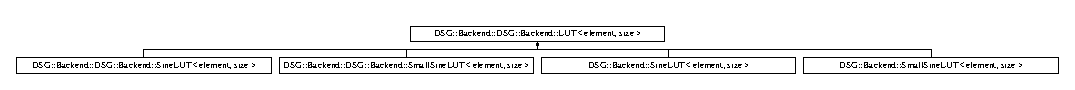
\includegraphics[height=0.758808cm]{classDSG_1_1Backend_1_1DSG_1_1Backend_1_1LUT}
\end{center}
\end{figure}
\subsection*{Public Member Functions}
\begin{DoxyCompactItemize}
\item 
\hyperlink{classDSG_1_1Backend_1_1DSG_1_1Backend_1_1LUT_a1072d9fe7abd014fbcf26a695ac00291}{L\+U\+T} ()
\item 
virtual \hyperlink{classDSG_1_1Backend_1_1DSG_1_1Backend_1_1LUT_a85cf256bae4e918775afe7d4f2a07e2a}{$\sim$\+L\+U\+T} ()
\item 
element const \& \hyperlink{classDSG_1_1Backend_1_1DSG_1_1Backend_1_1LUT_acd6db2fa4eba392de1cbb4795f351f8a}{operator\mbox{[}$\,$\mbox{]}} (unsigned long const \&index)
\item 
virtual element \hyperlink{classDSG_1_1Backend_1_1DSG_1_1Backend_1_1LUT_a4cdb48ce3c472160931968739623f8ac}{operator()} (double const \&x)
\item 
unsigned long const \& \hyperlink{classDSG_1_1Backend_1_1DSG_1_1Backend_1_1LUT_a65daa6f46f978a64da1c86089847602d}{Size} () const 
\end{DoxyCompactItemize}
\subsection*{Protected Attributes}
\begin{DoxyCompactItemize}
\item 
element \hyperlink{classDSG_1_1Backend_1_1DSG_1_1Backend_1_1LUT_a427da4b7eccdfe25e3c1889a8c2fdea6}{\+\_\+table} \mbox{[}size\mbox{]}
\item 
const unsigned long \hyperlink{classDSG_1_1Backend_1_1DSG_1_1Backend_1_1LUT_aa48956aa4debf08fdb517cb751d3e01d}{\+\_\+size}
\end{DoxyCompactItemize}


\subsection{Detailed Description}
\subsubsection*{template$<$typename element, unsigned long size$>$class D\+S\+G\+::\+Backend\+::\+D\+S\+G\+::\+Backend\+::\+L\+U\+T$<$ element, size $>$}



Definition at line 20 of file Sin.\+h.



\subsection{Constructor \& Destructor Documentation}
\hypertarget{classDSG_1_1Backend_1_1DSG_1_1Backend_1_1LUT_a1072d9fe7abd014fbcf26a695ac00291}{\index{D\+S\+G\+::\+Backend\+::\+D\+S\+G\+::\+Backend\+::\+L\+U\+T@{D\+S\+G\+::\+Backend\+::\+D\+S\+G\+::\+Backend\+::\+L\+U\+T}!L\+U\+T@{L\+U\+T}}
\index{L\+U\+T@{L\+U\+T}!D\+S\+G\+::\+Backend\+::\+D\+S\+G\+::\+Backend\+::\+L\+U\+T@{D\+S\+G\+::\+Backend\+::\+D\+S\+G\+::\+Backend\+::\+L\+U\+T}}
\subsubsection[{L\+U\+T}]{\setlength{\rightskip}{0pt plus 5cm}template$<$typename element, unsigned long size$>$ {\bf D\+S\+G\+::\+Backend\+::\+D\+S\+G\+::\+Backend\+::\+L\+U\+T}$<$ element, size $>$\+::{\bf L\+U\+T} (
\begin{DoxyParamCaption}
{}
\end{DoxyParamCaption}
)\hspace{0.3cm}{\ttfamily [inline]}}}\label{classDSG_1_1Backend_1_1DSG_1_1Backend_1_1LUT_a1072d9fe7abd014fbcf26a695ac00291}


Definition at line 22 of file Sin.\+h.


\begin{DoxyCode}
33 \{
\end{DoxyCode}
\hypertarget{classDSG_1_1Backend_1_1DSG_1_1Backend_1_1LUT_a85cf256bae4e918775afe7d4f2a07e2a}{\index{D\+S\+G\+::\+Backend\+::\+D\+S\+G\+::\+Backend\+::\+L\+U\+T@{D\+S\+G\+::\+Backend\+::\+D\+S\+G\+::\+Backend\+::\+L\+U\+T}!````~L\+U\+T@{$\sim$\+L\+U\+T}}
\index{````~L\+U\+T@{$\sim$\+L\+U\+T}!D\+S\+G\+::\+Backend\+::\+D\+S\+G\+::\+Backend\+::\+L\+U\+T@{D\+S\+G\+::\+Backend\+::\+D\+S\+G\+::\+Backend\+::\+L\+U\+T}}
\subsubsection[{$\sim$\+L\+U\+T}]{\setlength{\rightskip}{0pt plus 5cm}template$<$typename element, unsigned long size$>$ virtual {\bf D\+S\+G\+::\+Backend\+::\+D\+S\+G\+::\+Backend\+::\+L\+U\+T}$<$ element, size $>$\+::$\sim${\bf L\+U\+T} (
\begin{DoxyParamCaption}
{}
\end{DoxyParamCaption}
)\hspace{0.3cm}{\ttfamily [inline]}, {\ttfamily [virtual]}}}\label{classDSG_1_1Backend_1_1DSG_1_1Backend_1_1LUT_a85cf256bae4e918775afe7d4f2a07e2a}


Definition at line 23 of file Sin.\+h.


\begin{DoxyCode}
33 \{
\end{DoxyCode}


\subsection{Member Function Documentation}
\hypertarget{classDSG_1_1Backend_1_1DSG_1_1Backend_1_1LUT_a4cdb48ce3c472160931968739623f8ac}{\index{D\+S\+G\+::\+Backend\+::\+D\+S\+G\+::\+Backend\+::\+L\+U\+T@{D\+S\+G\+::\+Backend\+::\+D\+S\+G\+::\+Backend\+::\+L\+U\+T}!operator()@{operator()}}
\index{operator()@{operator()}!D\+S\+G\+::\+Backend\+::\+D\+S\+G\+::\+Backend\+::\+L\+U\+T@{D\+S\+G\+::\+Backend\+::\+D\+S\+G\+::\+Backend\+::\+L\+U\+T}}
\subsubsection[{operator()}]{\setlength{\rightskip}{0pt plus 5cm}template$<$typename element, unsigned long size$>$ virtual element {\bf D\+S\+G\+::\+Backend\+::\+D\+S\+G\+::\+Backend\+::\+L\+U\+T}$<$ element, size $>$\+::operator() (
\begin{DoxyParamCaption}
\item[{double const \&}]{x}
\end{DoxyParamCaption}
)\hspace{0.3cm}{\ttfamily [inline]}, {\ttfamily [virtual]}}}\label{classDSG_1_1Backend_1_1DSG_1_1Backend_1_1LUT_a4cdb48ce3c472160931968739623f8ac}


Reimplemented in \hyperlink{classDSG_1_1Backend_1_1DSG_1_1Backend_1_1SmallSineLUT_3_01int32__t_00_01size_01_4_a6093cb33233f44ac97d15998dc0ba005}{D\+S\+G\+::\+Backend\+::\+D\+S\+G\+::\+Backend\+::\+Small\+Sine\+L\+U\+T$<$ int32\+\_\+t, size $>$}, \hyperlink{classDSG_1_1Backend_1_1SmallSineLUT_3_01int32__t_00_01size_01_4_af8b347ef429ec5b6edbe7b752a003d2e}{D\+S\+G\+::\+Backend\+::\+Small\+Sine\+L\+U\+T$<$ int32\+\_\+t, size $>$}, \hyperlink{classDSG_1_1Backend_1_1DSG_1_1Backend_1_1SmallSineLUT_a2e15ffae0786ecc7a87d1202c5080850}{D\+S\+G\+::\+Backend\+::\+D\+S\+G\+::\+Backend\+::\+Small\+Sine\+L\+U\+T$<$ element, size $>$}, \hyperlink{classDSG_1_1Backend_1_1SmallSineLUT_af4b947cb0760ade07b788dae2472f4c0}{D\+S\+G\+::\+Backend\+::\+Small\+Sine\+L\+U\+T$<$ element, size $>$}, \hyperlink{classDSG_1_1Backend_1_1DSG_1_1Backend_1_1SineLUT_aaa841c0b14ec2a470d18932b816f78e6}{D\+S\+G\+::\+Backend\+::\+D\+S\+G\+::\+Backend\+::\+Sine\+L\+U\+T$<$ element, size $>$}, and \hyperlink{classDSG_1_1Backend_1_1SineLUT_a3d8ccd4f4ad7326100577346f0eb7e9b}{D\+S\+G\+::\+Backend\+::\+Sine\+L\+U\+T$<$ element, size $>$}.



Definition at line 30 of file Sin.\+h.


\begin{DoxyCode}
33                                         \{
\end{DoxyCode}
\hypertarget{classDSG_1_1Backend_1_1DSG_1_1Backend_1_1LUT_acd6db2fa4eba392de1cbb4795f351f8a}{\index{D\+S\+G\+::\+Backend\+::\+D\+S\+G\+::\+Backend\+::\+L\+U\+T@{D\+S\+G\+::\+Backend\+::\+D\+S\+G\+::\+Backend\+::\+L\+U\+T}!operator\mbox{[}$\,$\mbox{]}@{operator[]}}
\index{operator\mbox{[}$\,$\mbox{]}@{operator[]}!D\+S\+G\+::\+Backend\+::\+D\+S\+G\+::\+Backend\+::\+L\+U\+T@{D\+S\+G\+::\+Backend\+::\+D\+S\+G\+::\+Backend\+::\+L\+U\+T}}
\subsubsection[{operator[]}]{\setlength{\rightskip}{0pt plus 5cm}template$<$typename element, unsigned long size$>$ element const\& {\bf D\+S\+G\+::\+Backend\+::\+D\+S\+G\+::\+Backend\+::\+L\+U\+T}$<$ element, size $>$\+::operator\mbox{[}$\,$\mbox{]} (
\begin{DoxyParamCaption}
\item[{unsigned long const \&}]{index}
\end{DoxyParamCaption}
)\hspace{0.3cm}{\ttfamily [inline]}}}\label{classDSG_1_1Backend_1_1DSG_1_1Backend_1_1LUT_acd6db2fa4eba392de1cbb4795f351f8a}


Definition at line 24 of file Sin.\+h.


\begin{DoxyCode}
33                                         \{
\end{DoxyCode}
\hypertarget{classDSG_1_1Backend_1_1DSG_1_1Backend_1_1LUT_a65daa6f46f978a64da1c86089847602d}{\index{D\+S\+G\+::\+Backend\+::\+D\+S\+G\+::\+Backend\+::\+L\+U\+T@{D\+S\+G\+::\+Backend\+::\+D\+S\+G\+::\+Backend\+::\+L\+U\+T}!Size@{Size}}
\index{Size@{Size}!D\+S\+G\+::\+Backend\+::\+D\+S\+G\+::\+Backend\+::\+L\+U\+T@{D\+S\+G\+::\+Backend\+::\+D\+S\+G\+::\+Backend\+::\+L\+U\+T}}
\subsubsection[{Size}]{\setlength{\rightskip}{0pt plus 5cm}template$<$typename element, unsigned long size$>$ unsigned long const\& {\bf D\+S\+G\+::\+Backend\+::\+D\+S\+G\+::\+Backend\+::\+L\+U\+T}$<$ element, size $>$\+::Size (
\begin{DoxyParamCaption}
{}
\end{DoxyParamCaption}
) const\hspace{0.3cm}{\ttfamily [inline]}}}\label{classDSG_1_1Backend_1_1DSG_1_1Backend_1_1LUT_a65daa6f46f978a64da1c86089847602d}


Definition at line 33 of file Sin.\+h.


\begin{DoxyCode}
33                                         \{
34         \textcolor{comment}{//phs 0-1}
35 \textcolor{preprocessor}{#if sin\_impl == sin\_native}
\end{DoxyCode}


\subsection{Member Data Documentation}
\hypertarget{classDSG_1_1Backend_1_1DSG_1_1Backend_1_1LUT_aa48956aa4debf08fdb517cb751d3e01d}{\index{D\+S\+G\+::\+Backend\+::\+D\+S\+G\+::\+Backend\+::\+L\+U\+T@{D\+S\+G\+::\+Backend\+::\+D\+S\+G\+::\+Backend\+::\+L\+U\+T}!\+\_\+size@{\+\_\+size}}
\index{\+\_\+size@{\+\_\+size}!D\+S\+G\+::\+Backend\+::\+D\+S\+G\+::\+Backend\+::\+L\+U\+T@{D\+S\+G\+::\+Backend\+::\+D\+S\+G\+::\+Backend\+::\+L\+U\+T}}
\subsubsection[{\+\_\+size}]{\setlength{\rightskip}{0pt plus 5cm}template$<$typename element, unsigned long size$>$ const unsigned long {\bf D\+S\+G\+::\+Backend\+::\+D\+S\+G\+::\+Backend\+::\+L\+U\+T}$<$ element, size $>$\+::\+\_\+size\hspace{0.3cm}{\ttfamily [protected]}}}\label{classDSG_1_1Backend_1_1DSG_1_1Backend_1_1LUT_aa48956aa4debf08fdb517cb751d3e01d}


Definition at line 38 of file Sin.\+h.

\hypertarget{classDSG_1_1Backend_1_1DSG_1_1Backend_1_1LUT_a427da4b7eccdfe25e3c1889a8c2fdea6}{\index{D\+S\+G\+::\+Backend\+::\+D\+S\+G\+::\+Backend\+::\+L\+U\+T@{D\+S\+G\+::\+Backend\+::\+D\+S\+G\+::\+Backend\+::\+L\+U\+T}!\+\_\+table@{\+\_\+table}}
\index{\+\_\+table@{\+\_\+table}!D\+S\+G\+::\+Backend\+::\+D\+S\+G\+::\+Backend\+::\+L\+U\+T@{D\+S\+G\+::\+Backend\+::\+D\+S\+G\+::\+Backend\+::\+L\+U\+T}}
\subsubsection[{\+\_\+table}]{\setlength{\rightskip}{0pt plus 5cm}template$<$typename element, unsigned long size$>$ element {\bf D\+S\+G\+::\+Backend\+::\+D\+S\+G\+::\+Backend\+::\+L\+U\+T}$<$ element, size $>$\+::\+\_\+table\mbox{[}size\mbox{]}\hspace{0.3cm}{\ttfamily [protected]}}}\label{classDSG_1_1Backend_1_1DSG_1_1Backend_1_1LUT_a427da4b7eccdfe25e3c1889a8c2fdea6}


Definition at line 37 of file Sin.\+h.



The documentation for this class was generated from the following file\+:\begin{DoxyCompactItemize}
\item 
/\+Users/alexanderzywicki/\+Documents/\+School\+\_\+\+Stuff/\+Fall\+\_\+2014/\+Digital\+\_\+\+Signal\+\_\+\+Generation\+\_\+and\+\_\+\+Analysis/src/include/\hyperlink{Sin_8h}{Sin.\+h}\end{DoxyCompactItemize}

\hypertarget{classDSG_1_1Backend_1_1LUT}{\section{D\+S\+G\+:\+:Backend\+:\+:L\+U\+T$<$ element, size $>$ Class Template Reference}
\label{classDSG_1_1Backend_1_1LUT}\index{D\+S\+G\+::\+Backend\+::\+L\+U\+T$<$ element, size $>$@{D\+S\+G\+::\+Backend\+::\+L\+U\+T$<$ element, size $>$}}
}


{\ttfamily \#include $<$L\+U\+T.\+h$>$}

\subsection*{Public Member Functions}
\begin{DoxyCompactItemize}
\item 
\hyperlink{classDSG_1_1Backend_1_1LUT_af1a9dbe842f12dbd64dd90553bb8da5a}{L\+U\+T} ()
\item 
virtual \hyperlink{classDSG_1_1Backend_1_1LUT_ad38fd365aacce7f082c68a9f9d84eeac}{$\sim$\+L\+U\+T} ()
\item 
element const \& \hyperlink{classDSG_1_1Backend_1_1LUT_a50d8304c33760ed566039ebf5657807c}{operator\mbox{[}$\,$\mbox{]}} (unsigned long const \&index)
\item 
virtual element \hyperlink{classDSG_1_1Backend_1_1LUT_aef937689f5204ad06ae7732a74b7ec22}{operator()} (double const \&x)
\item 
unsigned long const \& \hyperlink{classDSG_1_1Backend_1_1LUT_a988c07b5002e0aee6e490244b80c8830}{Size} () const 
\end{DoxyCompactItemize}
\subsection*{Protected Attributes}
\begin{DoxyCompactItemize}
\item 
element \hyperlink{classDSG_1_1Backend_1_1LUT_a23615428e84d6be4424c8b897866f253}{\+\_\+table} \mbox{[}size\mbox{]}
\item 
const unsigned long \hyperlink{classDSG_1_1Backend_1_1LUT_ae18fa23936c51c1bdbd21311c9f1054e}{\+\_\+size}
\end{DoxyCompactItemize}


\subsection{Detailed Description}
\subsubsection*{template$<$typename element, unsigned long size$>$class D\+S\+G\+::\+Backend\+::\+L\+U\+T$<$ element, size $>$}



Definition at line 19 of file L\+U\+T.\+h.



\subsection{Constructor \& Destructor Documentation}
\hypertarget{classDSG_1_1Backend_1_1LUT_af1a9dbe842f12dbd64dd90553bb8da5a}{\index{D\+S\+G\+::\+Backend\+::\+L\+U\+T@{D\+S\+G\+::\+Backend\+::\+L\+U\+T}!L\+U\+T@{L\+U\+T}}
\index{L\+U\+T@{L\+U\+T}!D\+S\+G\+::\+Backend\+::\+L\+U\+T@{D\+S\+G\+::\+Backend\+::\+L\+U\+T}}
\subsubsection[{L\+U\+T}]{\setlength{\rightskip}{0pt plus 5cm}template$<$typename element , unsigned long size$>$ {\bf D\+S\+G\+::\+Backend\+::\+L\+U\+T}$<$ element, size $>$\+::{\bf L\+U\+T} (
\begin{DoxyParamCaption}
{}
\end{DoxyParamCaption}
)\hspace{0.3cm}{\ttfamily [inline]}}}\label{classDSG_1_1Backend_1_1LUT_af1a9dbe842f12dbd64dd90553bb8da5a}


Definition at line 21 of file L\+U\+T.\+h.


\begin{DoxyCode}
21 :\hyperlink{classDSG_1_1Backend_1_1LUT_ae18fa23936c51c1bdbd21311c9f1054e}{\_size}(size)\{\}
\end{DoxyCode}
\hypertarget{classDSG_1_1Backend_1_1LUT_ad38fd365aacce7f082c68a9f9d84eeac}{\index{D\+S\+G\+::\+Backend\+::\+L\+U\+T@{D\+S\+G\+::\+Backend\+::\+L\+U\+T}!````~L\+U\+T@{$\sim$\+L\+U\+T}}
\index{````~L\+U\+T@{$\sim$\+L\+U\+T}!D\+S\+G\+::\+Backend\+::\+L\+U\+T@{D\+S\+G\+::\+Backend\+::\+L\+U\+T}}
\subsubsection[{$\sim$\+L\+U\+T}]{\setlength{\rightskip}{0pt plus 5cm}template$<$typename element , unsigned long size$>$ virtual {\bf D\+S\+G\+::\+Backend\+::\+L\+U\+T}$<$ element, size $>$\+::$\sim${\bf L\+U\+T} (
\begin{DoxyParamCaption}
{}
\end{DoxyParamCaption}
)\hspace{0.3cm}{\ttfamily [inline]}, {\ttfamily [virtual]}}}\label{classDSG_1_1Backend_1_1LUT_ad38fd365aacce7f082c68a9f9d84eeac}


Definition at line 22 of file L\+U\+T.\+h.


\begin{DoxyCode}
22 \{\}
\end{DoxyCode}


\subsection{Member Function Documentation}
\hypertarget{classDSG_1_1Backend_1_1LUT_aef937689f5204ad06ae7732a74b7ec22}{\index{D\+S\+G\+::\+Backend\+::\+L\+U\+T@{D\+S\+G\+::\+Backend\+::\+L\+U\+T}!operator()@{operator()}}
\index{operator()@{operator()}!D\+S\+G\+::\+Backend\+::\+L\+U\+T@{D\+S\+G\+::\+Backend\+::\+L\+U\+T}}
\subsubsection[{operator()}]{\setlength{\rightskip}{0pt plus 5cm}template$<$typename element , unsigned long size$>$ virtual element {\bf D\+S\+G\+::\+Backend\+::\+L\+U\+T}$<$ element, size $>$\+::operator() (
\begin{DoxyParamCaption}
\item[{double const \&}]{x}
\end{DoxyParamCaption}
)\hspace{0.3cm}{\ttfamily [inline]}, {\ttfamily [virtual]}}}\label{classDSG_1_1Backend_1_1LUT_aef937689f5204ad06ae7732a74b7ec22}


Definition at line 29 of file L\+U\+T.\+h.


\begin{DoxyCode}
29                                                                \{
30                 \textcolor{keywordflow}{return} 0;
31             \}
\end{DoxyCode}
\hypertarget{classDSG_1_1Backend_1_1LUT_a50d8304c33760ed566039ebf5657807c}{\index{D\+S\+G\+::\+Backend\+::\+L\+U\+T@{D\+S\+G\+::\+Backend\+::\+L\+U\+T}!operator\mbox{[}$\,$\mbox{]}@{operator[]}}
\index{operator\mbox{[}$\,$\mbox{]}@{operator[]}!D\+S\+G\+::\+Backend\+::\+L\+U\+T@{D\+S\+G\+::\+Backend\+::\+L\+U\+T}}
\subsubsection[{operator[]}]{\setlength{\rightskip}{0pt plus 5cm}template$<$typename element , unsigned long size$>$ element const\& {\bf D\+S\+G\+::\+Backend\+::\+L\+U\+T}$<$ element, size $>$\+::operator\mbox{[}$\,$\mbox{]} (
\begin{DoxyParamCaption}
\item[{unsigned long const \&}]{index}
\end{DoxyParamCaption}
)\hspace{0.3cm}{\ttfamily [inline]}}}\label{classDSG_1_1Backend_1_1LUT_a50d8304c33760ed566039ebf5657807c}


Definition at line 23 of file L\+U\+T.\+h.


\begin{DoxyCode}
23                                                                  \{
24 \textcolor{preprocessor}{#ifdef DEBUG}
25                 assert(index<\hyperlink{classDSG_1_1Backend_1_1LUT_ae18fa23936c51c1bdbd21311c9f1054e}{\_size});
26 \textcolor{preprocessor}{#endif}
27                 \textcolor{keywordflow}{return} \hyperlink{classDSG_1_1Backend_1_1LUT_a23615428e84d6be4424c8b897866f253}{\_table}[index];
28             \}
\end{DoxyCode}
\hypertarget{classDSG_1_1Backend_1_1LUT_a988c07b5002e0aee6e490244b80c8830}{\index{D\+S\+G\+::\+Backend\+::\+L\+U\+T@{D\+S\+G\+::\+Backend\+::\+L\+U\+T}!Size@{Size}}
\index{Size@{Size}!D\+S\+G\+::\+Backend\+::\+L\+U\+T@{D\+S\+G\+::\+Backend\+::\+L\+U\+T}}
\subsubsection[{Size}]{\setlength{\rightskip}{0pt plus 5cm}template$<$typename element , unsigned long size$>$ unsigned long const\& {\bf D\+S\+G\+::\+Backend\+::\+L\+U\+T}$<$ element, size $>$\+::Size (
\begin{DoxyParamCaption}
{}
\end{DoxyParamCaption}
) const\hspace{0.3cm}{\ttfamily [inline]}}}\label{classDSG_1_1Backend_1_1LUT_a988c07b5002e0aee6e490244b80c8830}


Definition at line 32 of file L\+U\+T.\+h.


\begin{DoxyCode}
32                                             \{
33                 \textcolor{keywordflow}{return} \hyperlink{classDSG_1_1Backend_1_1LUT_ae18fa23936c51c1bdbd21311c9f1054e}{\_size};
34             \}
\end{DoxyCode}


\subsection{Member Data Documentation}
\hypertarget{classDSG_1_1Backend_1_1LUT_ae18fa23936c51c1bdbd21311c9f1054e}{\index{D\+S\+G\+::\+Backend\+::\+L\+U\+T@{D\+S\+G\+::\+Backend\+::\+L\+U\+T}!\+\_\+size@{\+\_\+size}}
\index{\+\_\+size@{\+\_\+size}!D\+S\+G\+::\+Backend\+::\+L\+U\+T@{D\+S\+G\+::\+Backend\+::\+L\+U\+T}}
\subsubsection[{\+\_\+size}]{\setlength{\rightskip}{0pt plus 5cm}template$<$typename element , unsigned long size$>$ const unsigned long {\bf D\+S\+G\+::\+Backend\+::\+L\+U\+T}$<$ element, size $>$\+::\+\_\+size\hspace{0.3cm}{\ttfamily [protected]}}}\label{classDSG_1_1Backend_1_1LUT_ae18fa23936c51c1bdbd21311c9f1054e}


Definition at line 37 of file L\+U\+T.\+h.

\hypertarget{classDSG_1_1Backend_1_1LUT_a23615428e84d6be4424c8b897866f253}{\index{D\+S\+G\+::\+Backend\+::\+L\+U\+T@{D\+S\+G\+::\+Backend\+::\+L\+U\+T}!\+\_\+table@{\+\_\+table}}
\index{\+\_\+table@{\+\_\+table}!D\+S\+G\+::\+Backend\+::\+L\+U\+T@{D\+S\+G\+::\+Backend\+::\+L\+U\+T}}
\subsubsection[{\+\_\+table}]{\setlength{\rightskip}{0pt plus 5cm}template$<$typename element , unsigned long size$>$ element {\bf D\+S\+G\+::\+Backend\+::\+L\+U\+T}$<$ element, size $>$\+::\+\_\+table\mbox{[}size\mbox{]}\hspace{0.3cm}{\ttfamily [protected]}}}\label{classDSG_1_1Backend_1_1LUT_a23615428e84d6be4424c8b897866f253}


Definition at line 36 of file L\+U\+T.\+h.



The documentation for this class was generated from the following file\+:\begin{DoxyCompactItemize}
\item 
/\+Users/alexanderzywicki/\+Documents/\+School\+\_\+\+Stuff/\+Fall\+\_\+2014/\+Digital\+\_\+\+Signal\+\_\+\+Generation\+\_\+and\+\_\+\+Analysis/src/include/\hyperlink{LUT_8h}{L\+U\+T.\+h}\end{DoxyCompactItemize}

\hypertarget{classDSG_1_1minBLEP}{\section{D\+S\+G\+:\+:min\+B\+L\+E\+P Class Reference}
\label{classDSG_1_1minBLEP}\index{D\+S\+G\+::min\+B\+L\+E\+P@{D\+S\+G\+::min\+B\+L\+E\+P}}
}


See file $\sim$/\+Research/icmc01-\/hardsync.pdf for details of algorithm.  




{\ttfamily \#include $<$min\+B\+L\+E\+P.\+h$>$}

Inheritance diagram for D\+S\+G\+:\+:min\+B\+L\+E\+P\+:\begin{figure}[H]
\begin{center}
\leavevmode
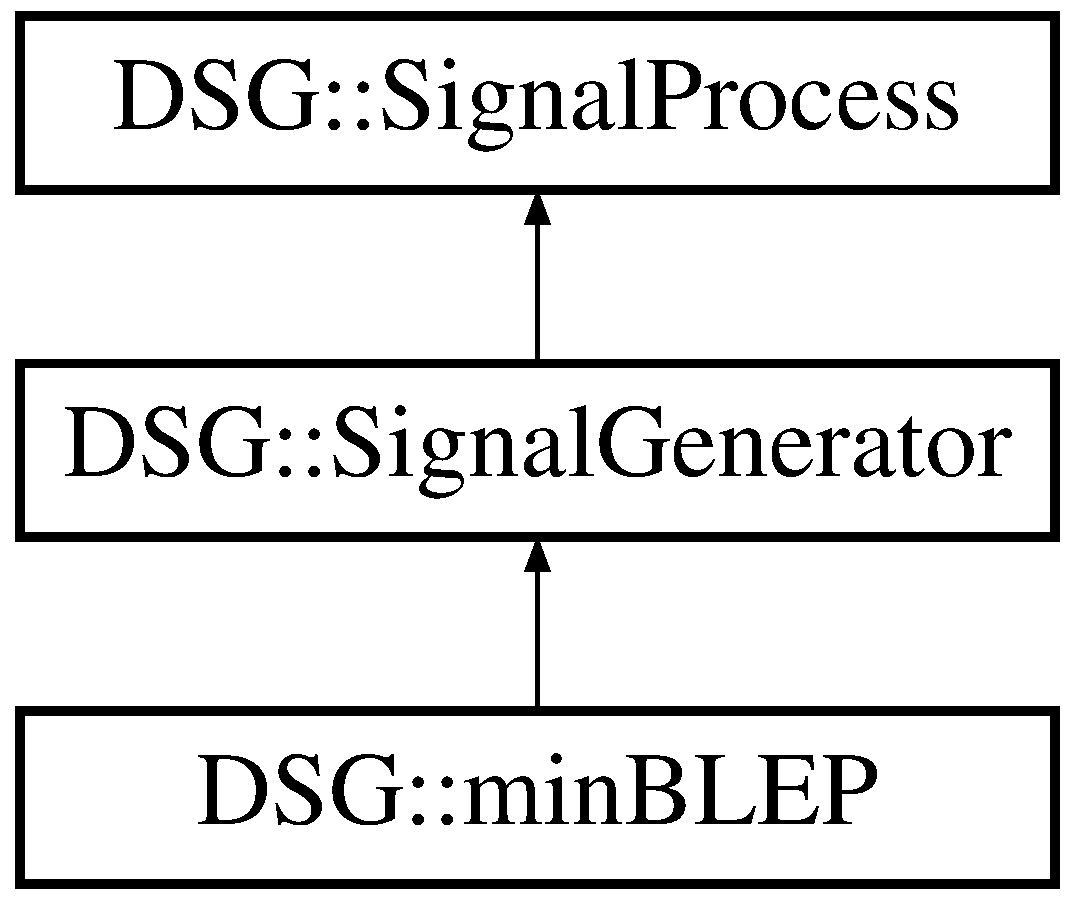
\includegraphics[height=3.000000cm]{classDSG_1_1minBLEP}
\end{center}
\end{figure}
\subsection*{Public Member Functions}
\begin{DoxyCompactItemize}
\item 
virtual bool \hyperlink{classDSG_1_1SignalGenerator_a95d485b68d874938ac93644b121607b9}{Perform} (\hyperlink{classDSG_1_1Sample}{Sample} \&signal)
\item 
virtual bool \hyperlink{classDSG_1_1SignalGenerator_abaa9aecd00b792d46166b91524b42db6}{Perform} (\hyperlink{classDSG_1_1RingBuffer}{Ring\+Buffer} \&signal)
\item 
virtual bool \hyperlink{classDSG_1_1SignalProcess_afdb8220100418893950c1161dd24db67}{Perform} (\hyperlink{classDSG_1_1Sample_aaf2e30d73911eccea99b53eeee15b612}{Sample\+::\+Sample} \&signal)=0
\item 
virtual double const \& \hyperlink{classDSG_1_1SignalGenerator_aedac746c5a70818d120858542ecb7c45}{Frequency} () const 
\item 
virtual double const \& \hyperlink{classDSG_1_1SignalGenerator_ae3ce8d45bafabbd86a0f535b15c3cd46}{Frequency} (double const \&value)
\item 
virtual double const \& \hyperlink{classDSG_1_1SignalGenerator_a1ce521847edd0b837fd840998f906b4b}{Phase\+Offset} () const 
\item 
virtual double const \& \hyperlink{classDSG_1_1SignalGenerator_a08b71b1f30ba65e629642c570291dc0e}{Phase\+Offset} (double const \&value)
\end{DoxyCompactItemize}
\subsection*{Protected Member Functions}
\begin{DoxyCompactItemize}
\item 
double \hyperlink{classDSG_1_1SignalGenerator_ac0d781b8673b3a283bf7c133290ede50}{\+\_\+pstep} ()
\item 
double \hyperlink{classDSG_1_1SignalGenerator_ae660eb4caa88b8d278f8d24d0908a487}{\+\_\+pstep\+\_\+rad} ()
\item 
void \hyperlink{classDSG_1_1SignalGenerator_a05baccb38d1e52860d4fcf7cb8430efc}{\+\_\+psync} ()
\end{DoxyCompactItemize}
\subsection*{Protected Attributes}
\begin{DoxyCompactItemize}
\item 
double \hyperlink{classDSG_1_1SignalGenerator_aa10f6c85d9adee901139ea7fb346f39d}{\+\_\+rate}
\item 
double \hyperlink{classDSG_1_1SignalGenerator_a67e296e3506dcdf09402c667cddff9ac}{\+\_\+frequency}
\item 
double \hyperlink{classDSG_1_1SignalGenerator_ac2271b582bf699275f077ecb642a8cd9}{\+\_\+phasor}
\end{DoxyCompactItemize}


\subsection{Detailed Description}
See file $\sim$/\+Research/icmc01-\/hardsync.pdf for details of algorithm. 

Definition at line 19 of file min\+B\+L\+E\+P.\+h.



\subsection{Member Function Documentation}
\hypertarget{classDSG_1_1SignalGenerator_ac0d781b8673b3a283bf7c133290ede50}{\index{D\+S\+G\+::min\+B\+L\+E\+P@{D\+S\+G\+::min\+B\+L\+E\+P}!\+\_\+pstep@{\+\_\+pstep}}
\index{\+\_\+pstep@{\+\_\+pstep}!D\+S\+G\+::min\+B\+L\+E\+P@{D\+S\+G\+::min\+B\+L\+E\+P}}
\subsubsection[{\+\_\+pstep}]{\setlength{\rightskip}{0pt plus 5cm}double D\+S\+G\+::\+Signal\+Generator\+::\+\_\+pstep (
\begin{DoxyParamCaption}
{}
\end{DoxyParamCaption}
)\hspace{0.3cm}{\ttfamily [inline]}, {\ttfamily [protected]}, {\ttfamily [inherited]}}}\label{classDSG_1_1SignalGenerator_ac0d781b8673b3a283bf7c133290ede50}


Definition at line 64 of file Signal\+Generator.\+h.


\begin{DoxyCode}
64                                          \{
65         value = \hyperlink{classDSG_1_1SignalGenerator_ac2271b582bf699275f077ecb642a8cd9}{\_phasor};
66         \hyperlink{classDSG_1_1SignalGenerator_ac2271b582bf699275f077ecb642a8cd9}{\_phasor}+=\hyperlink{classDSG_1_1SignalGenerator_aa10f6c85d9adee901139ea7fb346f39d}{\_rate};
67         \hyperlink{classDSG_1_1SignalGenerator_ac2271b582bf699275f077ecb642a8cd9}{\_phasor}>1?\hyperlink{classDSG_1_1SignalGenerator_ac2271b582bf699275f077ecb642a8cd9}{\_phasor}-=1:0;\textcolor{comment}{//cheaper cheaper %1}
68         \textcolor{comment}{//\_phasor -= (unsigned long)\_phasor;//cheaper %1}
69         \textcolor{keywordflow}{return} value;
70     \}
\end{DoxyCode}
\hypertarget{classDSG_1_1SignalGenerator_ae660eb4caa88b8d278f8d24d0908a487}{\index{D\+S\+G\+::min\+B\+L\+E\+P@{D\+S\+G\+::min\+B\+L\+E\+P}!\+\_\+pstep\+\_\+rad@{\+\_\+pstep\+\_\+rad}}
\index{\+\_\+pstep\+\_\+rad@{\+\_\+pstep\+\_\+rad}!D\+S\+G\+::min\+B\+L\+E\+P@{D\+S\+G\+::min\+B\+L\+E\+P}}
\subsubsection[{\+\_\+pstep\+\_\+rad}]{\setlength{\rightskip}{0pt plus 5cm}double D\+S\+G\+::\+Signal\+Generator\+::\+\_\+pstep\+\_\+rad (
\begin{DoxyParamCaption}
{}
\end{DoxyParamCaption}
)\hspace{0.3cm}{\ttfamily [inline]}, {\ttfamily [protected]}, {\ttfamily [inherited]}}}\label{classDSG_1_1SignalGenerator_ae660eb4caa88b8d278f8d24d0908a487}


Definition at line 71 of file Signal\+Generator.\+h.


\begin{DoxyCode}
71                                              \{
72         \textcolor{keywordflow}{return} \hyperlink{PI_8h_a4912c64aec0c943b7985db6cb61ff83a}{TWOPI} * \hyperlink{classDSG_1_1SignalGenerator_ac0d781b8673b3a283bf7c133290ede50}{\_pstep}();
73     \}
\end{DoxyCode}
\hypertarget{classDSG_1_1SignalGenerator_a05baccb38d1e52860d4fcf7cb8430efc}{\index{D\+S\+G\+::min\+B\+L\+E\+P@{D\+S\+G\+::min\+B\+L\+E\+P}!\+\_\+psync@{\+\_\+psync}}
\index{\+\_\+psync@{\+\_\+psync}!D\+S\+G\+::min\+B\+L\+E\+P@{D\+S\+G\+::min\+B\+L\+E\+P}}
\subsubsection[{\+\_\+psync}]{\setlength{\rightskip}{0pt plus 5cm}void D\+S\+G\+::\+Signal\+Generator\+::\+\_\+psync (
\begin{DoxyParamCaption}
{}
\end{DoxyParamCaption}
)\hspace{0.3cm}{\ttfamily [inline]}, {\ttfamily [protected]}, {\ttfamily [inherited]}}}\label{classDSG_1_1SignalGenerator_a05baccb38d1e52860d4fcf7cb8430efc}


Definition at line 74 of file Signal\+Generator.\+h.


\begin{DoxyCode}
74                                        \{
75         \hyperlink{classDSG_1_1SignalGenerator_ac2271b582bf699275f077ecb642a8cd9}{\_phasor} = \_phase\_offset;
76     \}
\end{DoxyCode}
\hypertarget{classDSG_1_1SignalGenerator_aedac746c5a70818d120858542ecb7c45}{\index{D\+S\+G\+::min\+B\+L\+E\+P@{D\+S\+G\+::min\+B\+L\+E\+P}!Frequency@{Frequency}}
\index{Frequency@{Frequency}!D\+S\+G\+::min\+B\+L\+E\+P@{D\+S\+G\+::min\+B\+L\+E\+P}}
\subsubsection[{Frequency}]{\setlength{\rightskip}{0pt plus 5cm}double const \& D\+S\+G\+::\+Signal\+Generator\+::\+Frequency (
\begin{DoxyParamCaption}
{}
\end{DoxyParamCaption}
) const\hspace{0.3cm}{\ttfamily [virtual]}, {\ttfamily [inherited]}}}\label{classDSG_1_1SignalGenerator_aedac746c5a70818d120858542ecb7c45}


Definition at line 16 of file Signal\+Generator.\+cpp.


\begin{DoxyCode}
16                                                 \{
17     \textcolor{keywordflow}{return} \hyperlink{classDSG_1_1SignalGenerator_a67e296e3506dcdf09402c667cddff9ac}{\_frequency};
18 \}
\end{DoxyCode}
\hypertarget{classDSG_1_1SignalGenerator_ae3ce8d45bafabbd86a0f535b15c3cd46}{\index{D\+S\+G\+::min\+B\+L\+E\+P@{D\+S\+G\+::min\+B\+L\+E\+P}!Frequency@{Frequency}}
\index{Frequency@{Frequency}!D\+S\+G\+::min\+B\+L\+E\+P@{D\+S\+G\+::min\+B\+L\+E\+P}}
\subsubsection[{Frequency}]{\setlength{\rightskip}{0pt plus 5cm}double const \& D\+S\+G\+::\+Signal\+Generator\+::\+Frequency (
\begin{DoxyParamCaption}
\item[{double const \&}]{value}
\end{DoxyParamCaption}
)\hspace{0.3cm}{\ttfamily [virtual]}, {\ttfamily [inherited]}}}\label{classDSG_1_1SignalGenerator_ae3ce8d45bafabbd86a0f535b15c3cd46}


Reimplemented in \hyperlink{classDSG_1_1BLIT_a67b698a54f37c361945cae3e137af76f}{D\+S\+G\+::\+B\+L\+I\+T}, \hyperlink{classDSG_1_1FourierSaw_a929602365c9b29f30f523fa07a29966e}{D\+S\+G\+::\+Fourier\+Saw}, \hyperlink{classDSG_1_1FourierSquare_a80f94eabad633e105cfa673fdee332d6}{D\+S\+G\+::\+Fourier\+Square}, and \hyperlink{classDSG_1_1FourierTriangle_aebb275eee9fb923636a8db5e4aa90b39}{D\+S\+G\+::\+Fourier\+Triangle}.



Definition at line 19 of file Signal\+Generator.\+cpp.


\begin{DoxyCode}
19                                                               \{
20     \hyperlink{classDSG_1_1SignalGenerator_a67e296e3506dcdf09402c667cddff9ac}{\_frequency} = value;
21     \hyperlink{classDSG_1_1SignalGenerator_aa10f6c85d9adee901139ea7fb346f39d}{\_rate} = \hyperlink{classDSG_1_1SignalGenerator_a67e296e3506dcdf09402c667cddff9ac}{\_frequency}/ \hyperlink{namespaceDSG_a0c5c3a251b3688398da18138c5efe4bf}{Sample\_Rate}();
22     \textcolor{keywordflow}{return} \hyperlink{classDSG_1_1SignalGenerator_a67e296e3506dcdf09402c667cddff9ac}{\_frequency};
23 \}
\end{DoxyCode}
\hypertarget{classDSG_1_1SignalGenerator_a95d485b68d874938ac93644b121607b9}{\index{D\+S\+G\+::min\+B\+L\+E\+P@{D\+S\+G\+::min\+B\+L\+E\+P}!Perform@{Perform}}
\index{Perform@{Perform}!D\+S\+G\+::min\+B\+L\+E\+P@{D\+S\+G\+::min\+B\+L\+E\+P}}
\subsubsection[{Perform}]{\setlength{\rightskip}{0pt plus 5cm}bool D\+S\+G\+::\+Signal\+Generator\+::\+Perform (
\begin{DoxyParamCaption}
\item[{{\bf Sample} \&}]{signal}
\end{DoxyParamCaption}
)\hspace{0.3cm}{\ttfamily [inline]}, {\ttfamily [virtual]}, {\ttfamily [inherited]}}}\label{classDSG_1_1SignalGenerator_a95d485b68d874938ac93644b121607b9}


Reimplemented in \hyperlink{classDSG_1_1FourierGenerator_a7f5e34e65c1fe757318fb5b063dabde9}{D\+S\+G\+::\+Fourier\+Generator}, \hyperlink{classDSG_1_1BLIT_a0f769ac63ee884a6d3899b38d6c2944c}{D\+S\+G\+::\+B\+L\+I\+T}, \hyperlink{classDSG_1_1AnalogGenerator_ac50033964304239b514b7ee9d064bc75}{D\+S\+G\+::\+Analog\+Generator}, \hyperlink{classDSG_1_1FourierSaw_a3cc372cd7dd694f8b9cb70e504dd04a1}{D\+S\+G\+::\+Fourier\+Saw}, \hyperlink{classDSG_1_1FourierSquare_a3e9cfc95b3592eaf04fbcd61a3c68387}{D\+S\+G\+::\+Fourier\+Square}, \hyperlink{classDSG_1_1FourierTriangle_ae927efb96f8d40f620dd02bdaaeef4d5}{D\+S\+G\+::\+Fourier\+Triangle}, \hyperlink{classDSG_1_1Sine_a04d925dc8c9a4b320f21697ce853a407}{D\+S\+G\+::\+Sine}, \hyperlink{classDSG_1_1AnalogSaw_ae52d07d0d03f6f1fb92c012cc52ae3eb}{D\+S\+G\+::\+Analog\+Saw}, \hyperlink{classDSG_1_1AnalogSquare_a93a4b464545a32f72491d3df490fd3f7}{D\+S\+G\+::\+Analog\+Square}, and \hyperlink{classDSG_1_1AnalogTriangle_ac3edb87c395763d6894672b471850b05}{D\+S\+G\+::\+Analog\+Triangle}.



Definition at line 56 of file Signal\+Generator.\+h.


\begin{DoxyCode}
56                                                        \{
57         signal = 0;
58         \textcolor{keywordflow}{return} \textcolor{keyword}{false};
59     \}
\end{DoxyCode}
\hypertarget{classDSG_1_1SignalGenerator_abaa9aecd00b792d46166b91524b42db6}{\index{D\+S\+G\+::min\+B\+L\+E\+P@{D\+S\+G\+::min\+B\+L\+E\+P}!Perform@{Perform}}
\index{Perform@{Perform}!D\+S\+G\+::min\+B\+L\+E\+P@{D\+S\+G\+::min\+B\+L\+E\+P}}
\subsubsection[{Perform}]{\setlength{\rightskip}{0pt plus 5cm}bool D\+S\+G\+::\+Signal\+Generator\+::\+Perform (
\begin{DoxyParamCaption}
\item[{{\bf Ring\+Buffer} \&}]{signal}
\end{DoxyParamCaption}
)\hspace{0.3cm}{\ttfamily [inline]}, {\ttfamily [virtual]}, {\ttfamily [inherited]}}}\label{classDSG_1_1SignalGenerator_abaa9aecd00b792d46166b91524b42db6}


Implements \hyperlink{classDSG_1_1SignalProcess_a9df44fe60cca01c3c697283408cecf4d}{D\+S\+G\+::\+Signal\+Process}.



Reimplemented in \hyperlink{classDSG_1_1FourierGenerator_a8b2aca91155dbb524aaf13867f273188}{D\+S\+G\+::\+Fourier\+Generator}, \hyperlink{classDSG_1_1BLIT_ae464457074d366c46f42b53b59d82ecb}{D\+S\+G\+::\+B\+L\+I\+T}, \hyperlink{classDSG_1_1AnalogGenerator_a1b4f1d4af926fcc3e9571db7960c8706}{D\+S\+G\+::\+Analog\+Generator}, \hyperlink{classDSG_1_1FourierSaw_a76b78874feebbc89d00656fec4bfd57a}{D\+S\+G\+::\+Fourier\+Saw}, \hyperlink{classDSG_1_1FourierSquare_ad9999119d9efc453329ed4b3eaf5f226}{D\+S\+G\+::\+Fourier\+Square}, \hyperlink{classDSG_1_1FourierTriangle_a017e2b59123ff3afa9a5c0e833e5f482}{D\+S\+G\+::\+Fourier\+Triangle}, \hyperlink{classDSG_1_1Sine_a6408fedf61f1f2a4026261d181997afc}{D\+S\+G\+::\+Sine}, \hyperlink{classDSG_1_1AnalogSaw_a14dbd5c7faf6559b9ea79f8eb1ad6af5}{D\+S\+G\+::\+Analog\+Saw}, \hyperlink{classDSG_1_1AnalogSquare_a1d9c8a380775a7e4f6e0aa8fb1b05af6}{D\+S\+G\+::\+Analog\+Square}, and \hyperlink{classDSG_1_1AnalogTriangle_a9456183af28d98ccf3daa85b8ad12b52}{D\+S\+G\+::\+Analog\+Triangle}.



Definition at line 60 of file Signal\+Generator.\+h.


\begin{DoxyCode}
60                                                            \{
61         signal.Flush();
62         \textcolor{keywordflow}{return} \textcolor{keyword}{false};
63     \}
\end{DoxyCode}
\hypertarget{classDSG_1_1SignalProcess_afdb8220100418893950c1161dd24db67}{\index{D\+S\+G\+::min\+B\+L\+E\+P@{D\+S\+G\+::min\+B\+L\+E\+P}!Perform@{Perform}}
\index{Perform@{Perform}!D\+S\+G\+::min\+B\+L\+E\+P@{D\+S\+G\+::min\+B\+L\+E\+P}}
\subsubsection[{Perform}]{\setlength{\rightskip}{0pt plus 5cm}virtual bool D\+S\+G\+::\+Signal\+Process\+::\+Perform (
\begin{DoxyParamCaption}
\item[{{\bf Sample\+::\+Sample} \&}]{signal}
\end{DoxyParamCaption}
)\hspace{0.3cm}{\ttfamily [inline]}, {\ttfamily [pure virtual]}, {\ttfamily [inherited]}}}\label{classDSG_1_1SignalProcess_afdb8220100418893950c1161dd24db67}
\hypertarget{classDSG_1_1SignalGenerator_a1ce521847edd0b837fd840998f906b4b}{\index{D\+S\+G\+::min\+B\+L\+E\+P@{D\+S\+G\+::min\+B\+L\+E\+P}!Phase\+Offset@{Phase\+Offset}}
\index{Phase\+Offset@{Phase\+Offset}!D\+S\+G\+::min\+B\+L\+E\+P@{D\+S\+G\+::min\+B\+L\+E\+P}}
\subsubsection[{Phase\+Offset}]{\setlength{\rightskip}{0pt plus 5cm}double const \& D\+S\+G\+::\+Signal\+Generator\+::\+Phase\+Offset (
\begin{DoxyParamCaption}
{}
\end{DoxyParamCaption}
) const\hspace{0.3cm}{\ttfamily [virtual]}, {\ttfamily [inherited]}}}\label{classDSG_1_1SignalGenerator_a1ce521847edd0b837fd840998f906b4b}


Definition at line 24 of file Signal\+Generator.\+cpp.


\begin{DoxyCode}
24                                                   \{
25     \textcolor{keywordflow}{return} \_phase\_offset;
26 \}
\end{DoxyCode}
\hypertarget{classDSG_1_1SignalGenerator_a08b71b1f30ba65e629642c570291dc0e}{\index{D\+S\+G\+::min\+B\+L\+E\+P@{D\+S\+G\+::min\+B\+L\+E\+P}!Phase\+Offset@{Phase\+Offset}}
\index{Phase\+Offset@{Phase\+Offset}!D\+S\+G\+::min\+B\+L\+E\+P@{D\+S\+G\+::min\+B\+L\+E\+P}}
\subsubsection[{Phase\+Offset}]{\setlength{\rightskip}{0pt plus 5cm}double const \& D\+S\+G\+::\+Signal\+Generator\+::\+Phase\+Offset (
\begin{DoxyParamCaption}
\item[{double const \&}]{value}
\end{DoxyParamCaption}
)\hspace{0.3cm}{\ttfamily [virtual]}, {\ttfamily [inherited]}}}\label{classDSG_1_1SignalGenerator_a08b71b1f30ba65e629642c570291dc0e}


Definition at line 27 of file Signal\+Generator.\+cpp.


\begin{DoxyCode}
27                                                                 \{
28     \_phase\_offset-=value;
29     \hyperlink{classDSG_1_1SignalGenerator_ac2271b582bf699275f077ecb642a8cd9}{\_phasor}-=\_phase\_offset;
30     \_phase\_offset=value;
31     \textcolor{keywordflow}{return} \_phase\_offset;
32 \}
\end{DoxyCode}


\subsection{Member Data Documentation}
\hypertarget{classDSG_1_1SignalGenerator_a67e296e3506dcdf09402c667cddff9ac}{\index{D\+S\+G\+::min\+B\+L\+E\+P@{D\+S\+G\+::min\+B\+L\+E\+P}!\+\_\+frequency@{\+\_\+frequency}}
\index{\+\_\+frequency@{\+\_\+frequency}!D\+S\+G\+::min\+B\+L\+E\+P@{D\+S\+G\+::min\+B\+L\+E\+P}}
\subsubsection[{\+\_\+frequency}]{\setlength{\rightskip}{0pt plus 5cm}double D\+S\+G\+::\+Signal\+Generator\+::\+\_\+frequency\hspace{0.3cm}{\ttfamily [protected]}, {\ttfamily [inherited]}}}\label{classDSG_1_1SignalGenerator_a67e296e3506dcdf09402c667cddff9ac}


Definition at line 34 of file Signal\+Generator.\+h.

\hypertarget{classDSG_1_1SignalGenerator_ac2271b582bf699275f077ecb642a8cd9}{\index{D\+S\+G\+::min\+B\+L\+E\+P@{D\+S\+G\+::min\+B\+L\+E\+P}!\+\_\+phasor@{\+\_\+phasor}}
\index{\+\_\+phasor@{\+\_\+phasor}!D\+S\+G\+::min\+B\+L\+E\+P@{D\+S\+G\+::min\+B\+L\+E\+P}}
\subsubsection[{\+\_\+phasor}]{\setlength{\rightskip}{0pt plus 5cm}double D\+S\+G\+::\+Signal\+Generator\+::\+\_\+phasor\hspace{0.3cm}{\ttfamily [protected]}, {\ttfamily [inherited]}}}\label{classDSG_1_1SignalGenerator_ac2271b582bf699275f077ecb642a8cd9}


Definition at line 46 of file Signal\+Generator.\+h.

\hypertarget{classDSG_1_1SignalGenerator_aa10f6c85d9adee901139ea7fb346f39d}{\index{D\+S\+G\+::min\+B\+L\+E\+P@{D\+S\+G\+::min\+B\+L\+E\+P}!\+\_\+rate@{\+\_\+rate}}
\index{\+\_\+rate@{\+\_\+rate}!D\+S\+G\+::min\+B\+L\+E\+P@{D\+S\+G\+::min\+B\+L\+E\+P}}
\subsubsection[{\+\_\+rate}]{\setlength{\rightskip}{0pt plus 5cm}double D\+S\+G\+::\+Signal\+Generator\+::\+\_\+rate\hspace{0.3cm}{\ttfamily [protected]}, {\ttfamily [inherited]}}}\label{classDSG_1_1SignalGenerator_aa10f6c85d9adee901139ea7fb346f39d}


Definition at line 33 of file Signal\+Generator.\+h.



The documentation for this class was generated from the following file\+:\begin{DoxyCompactItemize}
\item 
/\+Users/alexanderzywicki/\+Documents/\+School\+\_\+\+Stuff/\+Fall\+\_\+2014/\+Digital\+\_\+\+Signal\+\_\+\+Generation\+\_\+and\+\_\+\+Analysis/src/include/\hyperlink{minBLEP_8h}{min\+B\+L\+E\+P.\+h}\end{DoxyCompactItemize}

\hypertarget{classDSG_1_1polyBLEP}{\section{D\+S\+G\+:\+:poly\+B\+L\+E\+P Class Reference}
\label{classDSG_1_1polyBLEP}\index{D\+S\+G\+::poly\+B\+L\+E\+P@{D\+S\+G\+::poly\+B\+L\+E\+P}}
}


See file $\sim$/\+Research/poly\+B\+L\+E\+P.rtf for links to deatils about algorithm.  




{\ttfamily \#include $<$poly\+B\+L\+E\+P.\+h$>$}

Inheritance diagram for D\+S\+G\+:\+:poly\+B\+L\+E\+P\+:\begin{figure}[H]
\begin{center}
\leavevmode
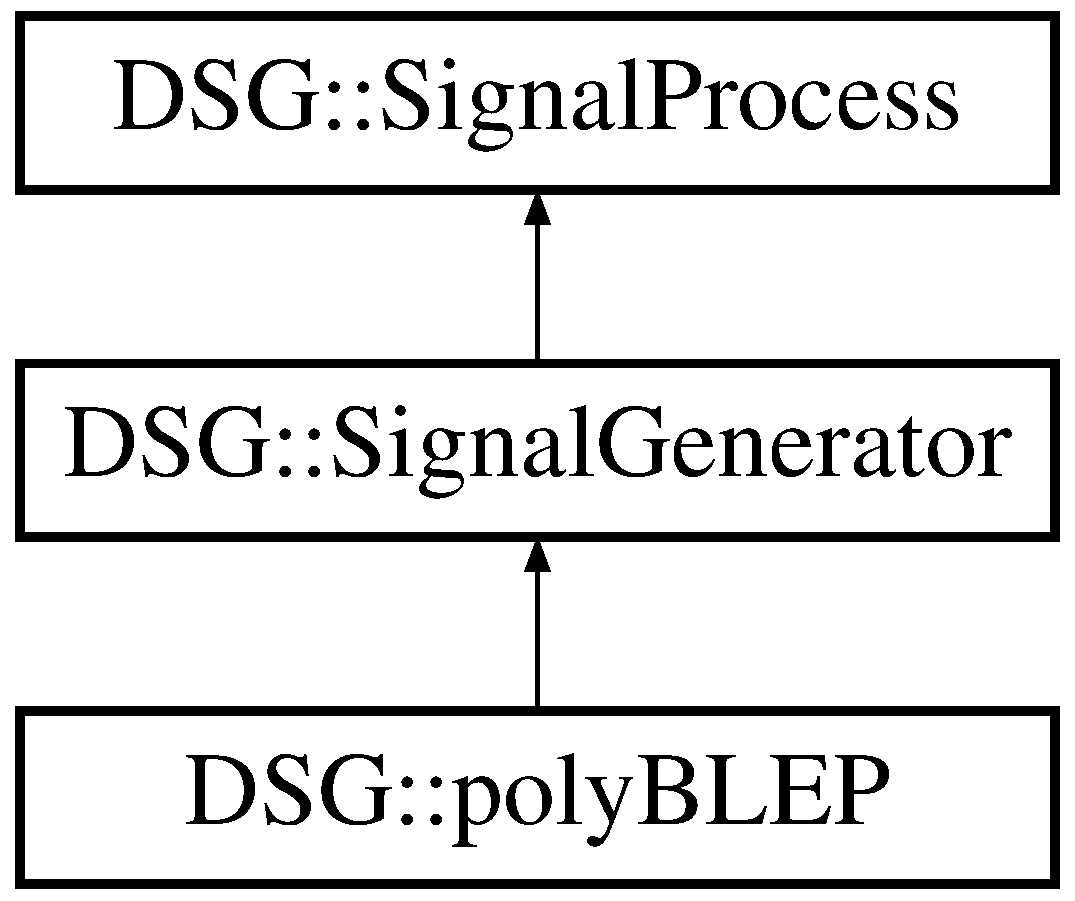
\includegraphics[height=3.000000cm]{classDSG_1_1polyBLEP}
\end{center}
\end{figure}
\subsection*{Public Member Functions}
\begin{DoxyCompactItemize}
\item 
virtual bool \hyperlink{classDSG_1_1SignalGenerator_a95d485b68d874938ac93644b121607b9}{Perform} (\hyperlink{classDSG_1_1Sample}{Sample} \&signal)
\item 
virtual bool \hyperlink{classDSG_1_1SignalGenerator_abaa9aecd00b792d46166b91524b42db6}{Perform} (\hyperlink{classDSG_1_1RingBuffer}{Ring\+Buffer} \&signal)
\item 
virtual bool \hyperlink{classDSG_1_1SignalProcess_afdb8220100418893950c1161dd24db67}{Perform} (\hyperlink{classDSG_1_1Sample_aaf2e30d73911eccea99b53eeee15b612}{Sample\+::\+Sample} \&signal)=0
\item 
virtual double const \& \hyperlink{classDSG_1_1SignalGenerator_aedac746c5a70818d120858542ecb7c45}{Frequency} () const 
\item 
virtual double const \& \hyperlink{classDSG_1_1SignalGenerator_ae3ce8d45bafabbd86a0f535b15c3cd46}{Frequency} (double const \&value)
\item 
virtual double const \& \hyperlink{classDSG_1_1SignalGenerator_a1ce521847edd0b837fd840998f906b4b}{Phase\+Offset} () const 
\item 
virtual double const \& \hyperlink{classDSG_1_1SignalGenerator_a08b71b1f30ba65e629642c570291dc0e}{Phase\+Offset} (double const \&value)
\end{DoxyCompactItemize}
\subsection*{Protected Member Functions}
\begin{DoxyCompactItemize}
\item 
double \hyperlink{classDSG_1_1SignalGenerator_ac0d781b8673b3a283bf7c133290ede50}{\+\_\+pstep} ()
\item 
double \hyperlink{classDSG_1_1SignalGenerator_ae660eb4caa88b8d278f8d24d0908a487}{\+\_\+pstep\+\_\+rad} ()
\item 
void \hyperlink{classDSG_1_1SignalGenerator_a05baccb38d1e52860d4fcf7cb8430efc}{\+\_\+psync} ()
\end{DoxyCompactItemize}
\subsection*{Protected Attributes}
\begin{DoxyCompactItemize}
\item 
double \hyperlink{classDSG_1_1SignalGenerator_aa10f6c85d9adee901139ea7fb346f39d}{\+\_\+rate}
\item 
double \hyperlink{classDSG_1_1SignalGenerator_a67e296e3506dcdf09402c667cddff9ac}{\+\_\+frequency}
\item 
double \hyperlink{classDSG_1_1SignalGenerator_ac2271b582bf699275f077ecb642a8cd9}{\+\_\+phasor}
\end{DoxyCompactItemize}


\subsection{Detailed Description}
See file $\sim$/\+Research/poly\+B\+L\+E\+P.rtf for links to deatils about algorithm. 

Definition at line 18 of file poly\+B\+L\+E\+P.\+h.



\subsection{Member Function Documentation}
\hypertarget{classDSG_1_1SignalGenerator_ac0d781b8673b3a283bf7c133290ede50}{\index{D\+S\+G\+::poly\+B\+L\+E\+P@{D\+S\+G\+::poly\+B\+L\+E\+P}!\+\_\+pstep@{\+\_\+pstep}}
\index{\+\_\+pstep@{\+\_\+pstep}!D\+S\+G\+::poly\+B\+L\+E\+P@{D\+S\+G\+::poly\+B\+L\+E\+P}}
\subsubsection[{\+\_\+pstep}]{\setlength{\rightskip}{0pt plus 5cm}double D\+S\+G\+::\+Signal\+Generator\+::\+\_\+pstep (
\begin{DoxyParamCaption}
{}
\end{DoxyParamCaption}
)\hspace{0.3cm}{\ttfamily [inline]}, {\ttfamily [protected]}, {\ttfamily [inherited]}}}\label{classDSG_1_1SignalGenerator_ac0d781b8673b3a283bf7c133290ede50}


Definition at line 52 of file Signal\+Generator.\+h.


\begin{DoxyCode}
52                                          \{
53         value = \hyperlink{classDSG_1_1SignalGenerator_ac2271b582bf699275f077ecb642a8cd9}{\_phasor};
54         \hyperlink{classDSG_1_1SignalGenerator_ac2271b582bf699275f077ecb642a8cd9}{\_phasor}+=\hyperlink{classDSG_1_1SignalGenerator_aa10f6c85d9adee901139ea7fb346f39d}{\_rate};
55         \hyperlink{classDSG_1_1SignalGenerator_ac2271b582bf699275f077ecb642a8cd9}{\_phasor}>1?\hyperlink{classDSG_1_1SignalGenerator_ac2271b582bf699275f077ecb642a8cd9}{\_phasor}-=1:0;\textcolor{comment}{//cheaper cheaper %1}
56         \textcolor{comment}{//\_phasor -= (unsigned long)\_phasor;//cheaper %1}
57         \textcolor{keywordflow}{return} value;
58     \}
\end{DoxyCode}
\hypertarget{classDSG_1_1SignalGenerator_ae660eb4caa88b8d278f8d24d0908a487}{\index{D\+S\+G\+::poly\+B\+L\+E\+P@{D\+S\+G\+::poly\+B\+L\+E\+P}!\+\_\+pstep\+\_\+rad@{\+\_\+pstep\+\_\+rad}}
\index{\+\_\+pstep\+\_\+rad@{\+\_\+pstep\+\_\+rad}!D\+S\+G\+::poly\+B\+L\+E\+P@{D\+S\+G\+::poly\+B\+L\+E\+P}}
\subsubsection[{\+\_\+pstep\+\_\+rad}]{\setlength{\rightskip}{0pt plus 5cm}double D\+S\+G\+::\+Signal\+Generator\+::\+\_\+pstep\+\_\+rad (
\begin{DoxyParamCaption}
{}
\end{DoxyParamCaption}
)\hspace{0.3cm}{\ttfamily [inline]}, {\ttfamily [protected]}, {\ttfamily [inherited]}}}\label{classDSG_1_1SignalGenerator_ae660eb4caa88b8d278f8d24d0908a487}


Definition at line 59 of file Signal\+Generator.\+h.


\begin{DoxyCode}
59                                              \{
60         \textcolor{keywordflow}{return} \hyperlink{PI_8h_a4912c64aec0c943b7985db6cb61ff83a}{TWOPI} * \hyperlink{classDSG_1_1SignalGenerator_ac0d781b8673b3a283bf7c133290ede50}{\_pstep}();
61     \}
\end{DoxyCode}
\hypertarget{classDSG_1_1SignalGenerator_a05baccb38d1e52860d4fcf7cb8430efc}{\index{D\+S\+G\+::poly\+B\+L\+E\+P@{D\+S\+G\+::poly\+B\+L\+E\+P}!\+\_\+psync@{\+\_\+psync}}
\index{\+\_\+psync@{\+\_\+psync}!D\+S\+G\+::poly\+B\+L\+E\+P@{D\+S\+G\+::poly\+B\+L\+E\+P}}
\subsubsection[{\+\_\+psync}]{\setlength{\rightskip}{0pt plus 5cm}void D\+S\+G\+::\+Signal\+Generator\+::\+\_\+psync (
\begin{DoxyParamCaption}
{}
\end{DoxyParamCaption}
)\hspace{0.3cm}{\ttfamily [inline]}, {\ttfamily [protected]}, {\ttfamily [inherited]}}}\label{classDSG_1_1SignalGenerator_a05baccb38d1e52860d4fcf7cb8430efc}


Definition at line 62 of file Signal\+Generator.\+h.


\begin{DoxyCode}
62                                        \{
63         \hyperlink{classDSG_1_1SignalGenerator_ac2271b582bf699275f077ecb642a8cd9}{\_phasor} = \_phase\_offset;
64     \}
\end{DoxyCode}
\hypertarget{classDSG_1_1SignalGenerator_aedac746c5a70818d120858542ecb7c45}{\index{D\+S\+G\+::poly\+B\+L\+E\+P@{D\+S\+G\+::poly\+B\+L\+E\+P}!Frequency@{Frequency}}
\index{Frequency@{Frequency}!D\+S\+G\+::poly\+B\+L\+E\+P@{D\+S\+G\+::poly\+B\+L\+E\+P}}
\subsubsection[{Frequency}]{\setlength{\rightskip}{0pt plus 5cm}double const \& D\+S\+G\+::\+Signal\+Generator\+::\+Frequency (
\begin{DoxyParamCaption}
{}
\end{DoxyParamCaption}
) const\hspace{0.3cm}{\ttfamily [virtual]}, {\ttfamily [inherited]}}}\label{classDSG_1_1SignalGenerator_aedac746c5a70818d120858542ecb7c45}


Definition at line 14 of file Signal\+Generator.\+cpp.


\begin{DoxyCode}
14                                                 \{
15     \textcolor{keywordflow}{return} \hyperlink{classDSG_1_1SignalGenerator_a67e296e3506dcdf09402c667cddff9ac}{\_frequency};
16 \}
\end{DoxyCode}
\hypertarget{classDSG_1_1SignalGenerator_ae3ce8d45bafabbd86a0f535b15c3cd46}{\index{D\+S\+G\+::poly\+B\+L\+E\+P@{D\+S\+G\+::poly\+B\+L\+E\+P}!Frequency@{Frequency}}
\index{Frequency@{Frequency}!D\+S\+G\+::poly\+B\+L\+E\+P@{D\+S\+G\+::poly\+B\+L\+E\+P}}
\subsubsection[{Frequency}]{\setlength{\rightskip}{0pt plus 5cm}double const \& D\+S\+G\+::\+Signal\+Generator\+::\+Frequency (
\begin{DoxyParamCaption}
\item[{double const \&}]{value}
\end{DoxyParamCaption}
)\hspace{0.3cm}{\ttfamily [virtual]}, {\ttfamily [inherited]}}}\label{classDSG_1_1SignalGenerator_ae3ce8d45bafabbd86a0f535b15c3cd46}


Reimplemented in \hyperlink{classDSG_1_1BLIT_a67b698a54f37c361945cae3e137af76f}{D\+S\+G\+::\+B\+L\+I\+T}, \hyperlink{classDSG_1_1FourierTriangle_aebb275eee9fb923636a8db5e4aa90b39}{D\+S\+G\+::\+Fourier\+Triangle}, \hyperlink{classDSG_1_1FourierSaw_a929602365c9b29f30f523fa07a29966e}{D\+S\+G\+::\+Fourier\+Saw}, and \hyperlink{classDSG_1_1FourierSquare_a80f94eabad633e105cfa673fdee332d6}{D\+S\+G\+::\+Fourier\+Square}.



Definition at line 17 of file Signal\+Generator.\+cpp.


\begin{DoxyCode}
17                                                               \{
18     \hyperlink{classDSG_1_1SignalGenerator_a67e296e3506dcdf09402c667cddff9ac}{\_frequency} = value;
19     \hyperlink{classDSG_1_1SignalGenerator_aa10f6c85d9adee901139ea7fb346f39d}{\_rate} = \hyperlink{classDSG_1_1SignalGenerator_a67e296e3506dcdf09402c667cddff9ac}{\_frequency}/ \hyperlink{namespaceDSG_a0c5c3a251b3688398da18138c5efe4bf}{Sample\_Rate}();
20     \textcolor{keywordflow}{return} \hyperlink{classDSG_1_1SignalGenerator_a67e296e3506dcdf09402c667cddff9ac}{\_frequency};
21 \}
\end{DoxyCode}
\hypertarget{classDSG_1_1SignalGenerator_a95d485b68d874938ac93644b121607b9}{\index{D\+S\+G\+::poly\+B\+L\+E\+P@{D\+S\+G\+::poly\+B\+L\+E\+P}!Perform@{Perform}}
\index{Perform@{Perform}!D\+S\+G\+::poly\+B\+L\+E\+P@{D\+S\+G\+::poly\+B\+L\+E\+P}}
\subsubsection[{Perform}]{\setlength{\rightskip}{0pt plus 5cm}bool D\+S\+G\+::\+Signal\+Generator\+::\+Perform (
\begin{DoxyParamCaption}
\item[{{\bf Sample} \&}]{signal}
\end{DoxyParamCaption}
)\hspace{0.3cm}{\ttfamily [inline]}, {\ttfamily [virtual]}, {\ttfamily [inherited]}}}\label{classDSG_1_1SignalGenerator_a95d485b68d874938ac93644b121607b9}


Reimplemented in \hyperlink{classDSG_1_1FourierGenerator_a7f5e34e65c1fe757318fb5b063dabde9}{D\+S\+G\+::\+Fourier\+Generator}, \hyperlink{classDSG_1_1BLIT_a0f769ac63ee884a6d3899b38d6c2944c}{D\+S\+G\+::\+B\+L\+I\+T}, \hyperlink{classDSG_1_1AnalogGenerator_ac50033964304239b514b7ee9d064bc75}{D\+S\+G\+::\+Analog\+Generator}, \hyperlink{classDSG_1_1FourierTriangle_ae927efb96f8d40f620dd02bdaaeef4d5}{D\+S\+G\+::\+Fourier\+Triangle}, \hyperlink{classDSG_1_1Sine_a04d925dc8c9a4b320f21697ce853a407}{D\+S\+G\+::\+Sine}, \hyperlink{classDSG_1_1FourierSaw_a3cc372cd7dd694f8b9cb70e504dd04a1}{D\+S\+G\+::\+Fourier\+Saw}, \hyperlink{classDSG_1_1AnalogSaw_ae52d07d0d03f6f1fb92c012cc52ae3eb}{D\+S\+G\+::\+Analog\+Saw}, \hyperlink{classDSG_1_1AnalogSquare_a93a4b464545a32f72491d3df490fd3f7}{D\+S\+G\+::\+Analog\+Square}, \hyperlink{classDSG_1_1AnalogTriangle_ac3edb87c395763d6894672b471850b05}{D\+S\+G\+::\+Analog\+Triangle}, and \hyperlink{classDSG_1_1FourierSquare_a3e9cfc95b3592eaf04fbcd61a3c68387}{D\+S\+G\+::\+Fourier\+Square}.



Definition at line 44 of file Signal\+Generator.\+h.


\begin{DoxyCode}
44                                                        \{
45         signal = 0;
46         \textcolor{keywordflow}{return} \textcolor{keyword}{false};
47     \}
\end{DoxyCode}
\hypertarget{classDSG_1_1SignalProcess_afdb8220100418893950c1161dd24db67}{\index{D\+S\+G\+::poly\+B\+L\+E\+P@{D\+S\+G\+::poly\+B\+L\+E\+P}!Perform@{Perform}}
\index{Perform@{Perform}!D\+S\+G\+::poly\+B\+L\+E\+P@{D\+S\+G\+::poly\+B\+L\+E\+P}}
\subsubsection[{Perform}]{\setlength{\rightskip}{0pt plus 5cm}virtual bool D\+S\+G\+::\+Signal\+Process\+::\+Perform (
\begin{DoxyParamCaption}
\item[{{\bf Sample\+::\+Sample} \&}]{signal}
\end{DoxyParamCaption}
)\hspace{0.3cm}{\ttfamily [inline]}, {\ttfamily [pure virtual]}, {\ttfamily [inherited]}}}\label{classDSG_1_1SignalProcess_afdb8220100418893950c1161dd24db67}
\hypertarget{classDSG_1_1SignalGenerator_abaa9aecd00b792d46166b91524b42db6}{\index{D\+S\+G\+::poly\+B\+L\+E\+P@{D\+S\+G\+::poly\+B\+L\+E\+P}!Perform@{Perform}}
\index{Perform@{Perform}!D\+S\+G\+::poly\+B\+L\+E\+P@{D\+S\+G\+::poly\+B\+L\+E\+P}}
\subsubsection[{Perform}]{\setlength{\rightskip}{0pt plus 5cm}bool D\+S\+G\+::\+Signal\+Generator\+::\+Perform (
\begin{DoxyParamCaption}
\item[{{\bf Ring\+Buffer} \&}]{signal}
\end{DoxyParamCaption}
)\hspace{0.3cm}{\ttfamily [inline]}, {\ttfamily [virtual]}, {\ttfamily [inherited]}}}\label{classDSG_1_1SignalGenerator_abaa9aecd00b792d46166b91524b42db6}


Implements \hyperlink{classDSG_1_1SignalProcess_a9df44fe60cca01c3c697283408cecf4d}{D\+S\+G\+::\+Signal\+Process}.



Reimplemented in \hyperlink{classDSG_1_1FourierGenerator_a8b2aca91155dbb524aaf13867f273188}{D\+S\+G\+::\+Fourier\+Generator}, \hyperlink{classDSG_1_1BLIT_ae464457074d366c46f42b53b59d82ecb}{D\+S\+G\+::\+B\+L\+I\+T}, \hyperlink{classDSG_1_1AnalogGenerator_a1b4f1d4af926fcc3e9571db7960c8706}{D\+S\+G\+::\+Analog\+Generator}, \hyperlink{classDSG_1_1FourierTriangle_a017e2b59123ff3afa9a5c0e833e5f482}{D\+S\+G\+::\+Fourier\+Triangle}, \hyperlink{classDSG_1_1Sine_a6408fedf61f1f2a4026261d181997afc}{D\+S\+G\+::\+Sine}, \hyperlink{classDSG_1_1FourierSaw_a76b78874feebbc89d00656fec4bfd57a}{D\+S\+G\+::\+Fourier\+Saw}, \hyperlink{classDSG_1_1AnalogSaw_a14dbd5c7faf6559b9ea79f8eb1ad6af5}{D\+S\+G\+::\+Analog\+Saw}, \hyperlink{classDSG_1_1AnalogSquare_a1d9c8a380775a7e4f6e0aa8fb1b05af6}{D\+S\+G\+::\+Analog\+Square}, \hyperlink{classDSG_1_1AnalogTriangle_a9456183af28d98ccf3daa85b8ad12b52}{D\+S\+G\+::\+Analog\+Triangle}, and \hyperlink{classDSG_1_1FourierSquare_ad9999119d9efc453329ed4b3eaf5f226}{D\+S\+G\+::\+Fourier\+Square}.



Definition at line 48 of file Signal\+Generator.\+h.


\begin{DoxyCode}
48                                                            \{
49         signal.Flush();
50         \textcolor{keywordflow}{return} \textcolor{keyword}{false};
51     \}
\end{DoxyCode}
\hypertarget{classDSG_1_1SignalGenerator_a1ce521847edd0b837fd840998f906b4b}{\index{D\+S\+G\+::poly\+B\+L\+E\+P@{D\+S\+G\+::poly\+B\+L\+E\+P}!Phase\+Offset@{Phase\+Offset}}
\index{Phase\+Offset@{Phase\+Offset}!D\+S\+G\+::poly\+B\+L\+E\+P@{D\+S\+G\+::poly\+B\+L\+E\+P}}
\subsubsection[{Phase\+Offset}]{\setlength{\rightskip}{0pt plus 5cm}double const \& D\+S\+G\+::\+Signal\+Generator\+::\+Phase\+Offset (
\begin{DoxyParamCaption}
{}
\end{DoxyParamCaption}
) const\hspace{0.3cm}{\ttfamily [virtual]}, {\ttfamily [inherited]}}}\label{classDSG_1_1SignalGenerator_a1ce521847edd0b837fd840998f906b4b}


Definition at line 22 of file Signal\+Generator.\+cpp.


\begin{DoxyCode}
22                                                   \{
23     \textcolor{keywordflow}{return} \_phase\_offset;
24 \}
\end{DoxyCode}
\hypertarget{classDSG_1_1SignalGenerator_a08b71b1f30ba65e629642c570291dc0e}{\index{D\+S\+G\+::poly\+B\+L\+E\+P@{D\+S\+G\+::poly\+B\+L\+E\+P}!Phase\+Offset@{Phase\+Offset}}
\index{Phase\+Offset@{Phase\+Offset}!D\+S\+G\+::poly\+B\+L\+E\+P@{D\+S\+G\+::poly\+B\+L\+E\+P}}
\subsubsection[{Phase\+Offset}]{\setlength{\rightskip}{0pt plus 5cm}double const \& D\+S\+G\+::\+Signal\+Generator\+::\+Phase\+Offset (
\begin{DoxyParamCaption}
\item[{double const \&}]{value}
\end{DoxyParamCaption}
)\hspace{0.3cm}{\ttfamily [virtual]}, {\ttfamily [inherited]}}}\label{classDSG_1_1SignalGenerator_a08b71b1f30ba65e629642c570291dc0e}


Definition at line 25 of file Signal\+Generator.\+cpp.


\begin{DoxyCode}
25                                                                 \{
26     \_phase\_offset-=value;
27     \hyperlink{classDSG_1_1SignalGenerator_ac2271b582bf699275f077ecb642a8cd9}{\_phasor}-=\_phase\_offset;
28     \_phase\_offset=value;
29     \textcolor{keywordflow}{return} \_phase\_offset;
30 \}\end{DoxyCode}


\subsection{Member Data Documentation}
\hypertarget{classDSG_1_1SignalGenerator_a67e296e3506dcdf09402c667cddff9ac}{\index{D\+S\+G\+::poly\+B\+L\+E\+P@{D\+S\+G\+::poly\+B\+L\+E\+P}!\+\_\+frequency@{\+\_\+frequency}}
\index{\+\_\+frequency@{\+\_\+frequency}!D\+S\+G\+::poly\+B\+L\+E\+P@{D\+S\+G\+::poly\+B\+L\+E\+P}}
\subsubsection[{\+\_\+frequency}]{\setlength{\rightskip}{0pt plus 5cm}double D\+S\+G\+::\+Signal\+Generator\+::\+\_\+frequency\hspace{0.3cm}{\ttfamily [protected]}, {\ttfamily [inherited]}}}\label{classDSG_1_1SignalGenerator_a67e296e3506dcdf09402c667cddff9ac}


Definition at line 28 of file Signal\+Generator.\+h.

\hypertarget{classDSG_1_1SignalGenerator_ac2271b582bf699275f077ecb642a8cd9}{\index{D\+S\+G\+::poly\+B\+L\+E\+P@{D\+S\+G\+::poly\+B\+L\+E\+P}!\+\_\+phasor@{\+\_\+phasor}}
\index{\+\_\+phasor@{\+\_\+phasor}!D\+S\+G\+::poly\+B\+L\+E\+P@{D\+S\+G\+::poly\+B\+L\+E\+P}}
\subsubsection[{\+\_\+phasor}]{\setlength{\rightskip}{0pt plus 5cm}double D\+S\+G\+::\+Signal\+Generator\+::\+\_\+phasor\hspace{0.3cm}{\ttfamily [protected]}, {\ttfamily [inherited]}}}\label{classDSG_1_1SignalGenerator_ac2271b582bf699275f077ecb642a8cd9}


Definition at line 38 of file Signal\+Generator.\+h.

\hypertarget{classDSG_1_1SignalGenerator_aa10f6c85d9adee901139ea7fb346f39d}{\index{D\+S\+G\+::poly\+B\+L\+E\+P@{D\+S\+G\+::poly\+B\+L\+E\+P}!\+\_\+rate@{\+\_\+rate}}
\index{\+\_\+rate@{\+\_\+rate}!D\+S\+G\+::poly\+B\+L\+E\+P@{D\+S\+G\+::poly\+B\+L\+E\+P}}
\subsubsection[{\+\_\+rate}]{\setlength{\rightskip}{0pt plus 5cm}double D\+S\+G\+::\+Signal\+Generator\+::\+\_\+rate\hspace{0.3cm}{\ttfamily [protected]}, {\ttfamily [inherited]}}}\label{classDSG_1_1SignalGenerator_aa10f6c85d9adee901139ea7fb346f39d}


Definition at line 27 of file Signal\+Generator.\+h.



The documentation for this class was generated from the following file\+:\begin{DoxyCompactItemize}
\item 
/\+Users/alexanderzywicki/\+Documents/\+School\+\_\+\+Stuff/\+Fall\+\_\+2014/\+Digital\+\_\+\+Signal\+\_\+\+Generation\+\_\+and\+\_\+\+Analysis/src/include/\hyperlink{polyBLEP_8h}{poly\+B\+L\+E\+P.\+h}\end{DoxyCompactItemize}

\hypertarget{classDSG_1_1Backend_1_1Queue}{\section{D\+S\+G\+:\+:Backend\+:\+:Queue$<$ element $>$ Class Template Reference}
\label{classDSG_1_1Backend_1_1Queue}\index{D\+S\+G\+::\+Backend\+::\+Queue$<$ element $>$@{D\+S\+G\+::\+Backend\+::\+Queue$<$ element $>$}}
}


{\ttfamily \#include $<$Queue.\+h$>$}

Inheritance diagram for D\+S\+G\+:\+:Backend\+:\+:Queue$<$ element $>$\+:\begin{figure}[H]
\begin{center}
\leavevmode
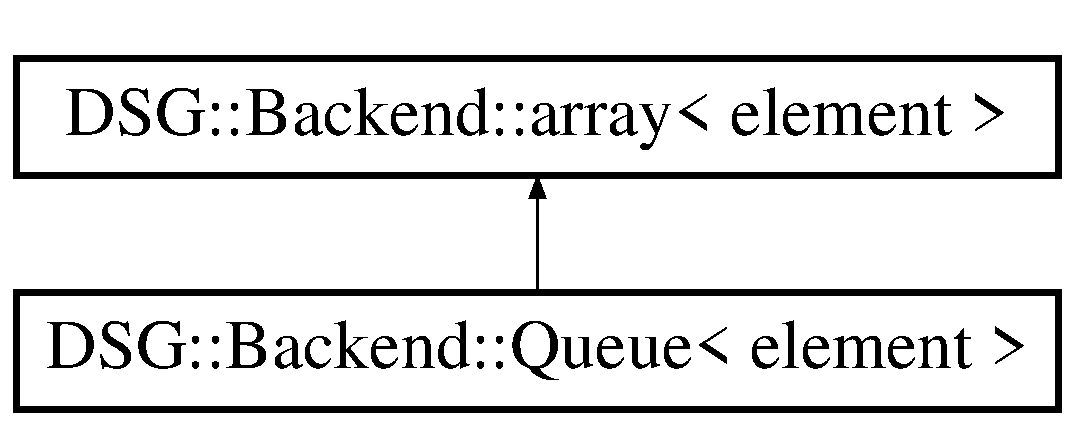
\includegraphics[height=2.000000cm]{classDSG_1_1Backend_1_1Queue}
\end{center}
\end{figure}
\subsection*{Public Types}
\begin{DoxyCompactItemize}
\item 
typedef element $\ast$ \hyperlink{classDSG_1_1Backend_1_1array_abfd0db2267892f4d2f397638faf85ca3}{pointer}
\item 
typedef element \& \hyperlink{classDSG_1_1Backend_1_1array_a8af2a20d445daee75e9e6b122498e0a6}{reference}
\end{DoxyCompactItemize}
\subsection*{Public Member Functions}
\begin{DoxyCompactItemize}
\item 
\hyperlink{classDSG_1_1Backend_1_1Queue_abf114ae1bb60464f072dcb755c48b87b}{Queue} ()
\item 
\hyperlink{classDSG_1_1Backend_1_1Queue_ac25736be535f1c1de655057899e309cd}{Queue} (unsigned long size)
\item 
\hyperlink{classDSG_1_1Backend_1_1Queue_a6f6299238080adc2630ad48180b45752}{Queue} (\hyperlink{classDSG_1_1Backend_1_1Queue}{Queue}$<$ element $>$ const \&other)
\item 
\hyperlink{classDSG_1_1Backend_1_1Queue}{Queue}$<$ element $>$ \& \hyperlink{classDSG_1_1Backend_1_1Queue_a0e8e1870d4a3034376fa6161ca86ed8c}{operator=} (\hyperlink{classDSG_1_1Backend_1_1Queue}{Queue}$<$ element $>$ const \&other)
\item 
virtual \hyperlink{classDSG_1_1Backend_1_1Queue_a95e3f62a9c0bfb6542fbdfbba50cb980}{$\sim$\+Queue} ()
\item 
bool \hyperlink{classDSG_1_1Backend_1_1Queue_a7b50e6db9134efc9b2b564cbec45c91f}{Write} (element const \&value)
\item 
bool \hyperlink{classDSG_1_1Backend_1_1Queue_ac79c16ed1070d092738f6cb4c525b4b1}{Read} (element \&place)
\item 
unsigned long const \& \hyperlink{classDSG_1_1Backend_1_1Queue_a15f58a6dfac40aabe6c0dc070269d8aa}{Count} () const 
\item 
bool \hyperlink{classDSG_1_1Backend_1_1Queue_a47abb536001453baa2db7caa4f0ccfea}{Full} () const 
\item 
bool \hyperlink{classDSG_1_1Backend_1_1Queue_aa2a871168b5d8eb9075d1506752046b0}{Empty} () const 
\item 
void \hyperlink{classDSG_1_1Backend_1_1Queue_ae78a96d54b37abff7a60d7941e84d8d8}{Flush} ()
\item 
element \& \hyperlink{classDSG_1_1Backend_1_1array_a69fb5ed051dd548a544f4d9ebd94fda7}{operator\mbox{[}$\,$\mbox{]}} (unsigned long const \&index)
\item 
unsigned long const \& \hyperlink{classDSG_1_1Backend_1_1array_ad31900d7cd043f7f058f7d86a36d1748}{Size} () const 
\end{DoxyCompactItemize}
\subsection*{Protected Member Functions}
\begin{DoxyCompactItemize}
\item 
unsigned long \hyperlink{classDSG_1_1Backend_1_1Queue_a2ca3705f53a9fa79663590e8bf939045}{next} (unsigned long value)
\item 
unsigned long \hyperlink{classDSG_1_1Backend_1_1Queue_a99c7fb1c0a319c1959dc2a9633fe5425}{make\+\_\+pow\+\_\+2} (unsigned long value)
\end{DoxyCompactItemize}
\subsection*{Protected Attributes}
\begin{DoxyCompactItemize}
\item 
std\+::atomic$<$ unsigned long $>$ \hyperlink{classDSG_1_1Backend_1_1Queue_adbbe7e332752d500e7b9fadeb08cac54}{\+\_\+write}
\item 
std\+::atomic$<$ unsigned long $>$ \hyperlink{classDSG_1_1Backend_1_1Queue_a10510513da0290a435fe47079287cf29}{\+\_\+read}
\item 
unsigned long \hyperlink{classDSG_1_1Backend_1_1Queue_ae2ec3926f9e8cbabd17dadb309bcc26f}{\+\_\+count}
\item 
unsigned long \hyperlink{classDSG_1_1Backend_1_1Queue_ad82aa028cc33db5cc22a4c478dabe399}{\+\_\+\+M\+A\+S\+K}
\item 
element $\ast$ \hyperlink{classDSG_1_1Backend_1_1array_a520f838f921d4f48852694e79da0564c}{\+\_\+array}
\item 
unsigned long \hyperlink{classDSG_1_1Backend_1_1array_a44349f32c09ebb31d5eadbe9a222cba2}{\+\_\+size}
\end{DoxyCompactItemize}


\subsection{Detailed Description}
\subsubsection*{template$<$class element$>$class D\+S\+G\+::\+Backend\+::\+Queue$<$ element $>$}



Definition at line 74 of file Queue.\+h.



\subsection{Member Typedef Documentation}
\hypertarget{classDSG_1_1Backend_1_1array_abfd0db2267892f4d2f397638faf85ca3}{\index{D\+S\+G\+::\+Backend\+::\+Queue@{D\+S\+G\+::\+Backend\+::\+Queue}!pointer@{pointer}}
\index{pointer@{pointer}!D\+S\+G\+::\+Backend\+::\+Queue@{D\+S\+G\+::\+Backend\+::\+Queue}}
\subsubsection[{pointer}]{\setlength{\rightskip}{0pt plus 5cm}template$<$class element$>$ typedef element$\ast$ {\bf D\+S\+G\+::\+Backend\+::array}$<$ element $>$\+::{\bf pointer}\hspace{0.3cm}{\ttfamily [inherited]}}}\label{classDSG_1_1Backend_1_1array_abfd0db2267892f4d2f397638faf85ca3}


Definition at line 29 of file Queue.\+h.

\hypertarget{classDSG_1_1Backend_1_1array_a8af2a20d445daee75e9e6b122498e0a6}{\index{D\+S\+G\+::\+Backend\+::\+Queue@{D\+S\+G\+::\+Backend\+::\+Queue}!reference@{reference}}
\index{reference@{reference}!D\+S\+G\+::\+Backend\+::\+Queue@{D\+S\+G\+::\+Backend\+::\+Queue}}
\subsubsection[{reference}]{\setlength{\rightskip}{0pt plus 5cm}template$<$class element$>$ typedef element\& {\bf D\+S\+G\+::\+Backend\+::array}$<$ element $>$\+::{\bf reference}\hspace{0.3cm}{\ttfamily [inherited]}}}\label{classDSG_1_1Backend_1_1array_a8af2a20d445daee75e9e6b122498e0a6}


Definition at line 30 of file Queue.\+h.



\subsection{Constructor \& Destructor Documentation}
\hypertarget{classDSG_1_1Backend_1_1Queue_abf114ae1bb60464f072dcb755c48b87b}{\index{D\+S\+G\+::\+Backend\+::\+Queue@{D\+S\+G\+::\+Backend\+::\+Queue}!Queue@{Queue}}
\index{Queue@{Queue}!D\+S\+G\+::\+Backend\+::\+Queue@{D\+S\+G\+::\+Backend\+::\+Queue}}
\subsubsection[{Queue}]{\setlength{\rightskip}{0pt plus 5cm}template$<$class element$>$ {\bf D\+S\+G\+::\+Backend\+::\+Queue}$<$ element $>$\+::{\bf Queue} (
\begin{DoxyParamCaption}
{}
\end{DoxyParamCaption}
)\hspace{0.3cm}{\ttfamily [inline]}}}\label{classDSG_1_1Backend_1_1Queue_abf114ae1bb60464f072dcb755c48b87b}


Definition at line 76 of file Queue.\+h.


\begin{DoxyCode}
76 :array<element>(0),\hyperlink{classDSG_1_1Backend_1_1Queue_a10510513da0290a435fe47079287cf29}{\_read}(0),\hyperlink{classDSG_1_1Backend_1_1Queue_adbbe7e332752d500e7b9fadeb08cac54}{\_write}(0),\hyperlink{classDSG_1_1Backend_1_1Queue_ae2ec3926f9e8cbabd17dadb309bcc26f}{\_count}(0),\hyperlink{classDSG_1_1Backend_1_1Queue_ad82aa028cc33db5cc22a4c478dabe399}{\_MASK}(0)\{\}
\end{DoxyCode}
\hypertarget{classDSG_1_1Backend_1_1Queue_ac25736be535f1c1de655057899e309cd}{\index{D\+S\+G\+::\+Backend\+::\+Queue@{D\+S\+G\+::\+Backend\+::\+Queue}!Queue@{Queue}}
\index{Queue@{Queue}!D\+S\+G\+::\+Backend\+::\+Queue@{D\+S\+G\+::\+Backend\+::\+Queue}}
\subsubsection[{Queue}]{\setlength{\rightskip}{0pt plus 5cm}template$<$class element$>$ {\bf D\+S\+G\+::\+Backend\+::\+Queue}$<$ element $>$\+::{\bf Queue} (
\begin{DoxyParamCaption}
\item[{unsigned long}]{size}
\end{DoxyParamCaption}
)\hspace{0.3cm}{\ttfamily [inline]}}}\label{classDSG_1_1Backend_1_1Queue_ac25736be535f1c1de655057899e309cd}


Definition at line 77 of file Queue.\+h.


\begin{DoxyCode}
77                                      :array<element>(\hyperlink{classDSG_1_1Backend_1_1Queue_a99c7fb1c0a319c1959dc2a9633fe5425}{make\_pow\_2}(size)),
      \hyperlink{classDSG_1_1Backend_1_1Queue_a10510513da0290a435fe47079287cf29}{\_read}(0),\hyperlink{classDSG_1_1Backend_1_1Queue_adbbe7e332752d500e7b9fadeb08cac54}{\_write}(0),\hyperlink{classDSG_1_1Backend_1_1Queue_ae2ec3926f9e8cbabd17dadb309bcc26f}{\_count}(0)\{
78                 \hyperlink{classDSG_1_1Backend_1_1Queue_ad82aa028cc33db5cc22a4c478dabe399}{\_MASK} = this->\hyperlink{classDSG_1_1Backend_1_1array_a44349f32c09ebb31d5eadbe9a222cba2}{\_size}-1;
79             \}
\end{DoxyCode}
\hypertarget{classDSG_1_1Backend_1_1Queue_a6f6299238080adc2630ad48180b45752}{\index{D\+S\+G\+::\+Backend\+::\+Queue@{D\+S\+G\+::\+Backend\+::\+Queue}!Queue@{Queue}}
\index{Queue@{Queue}!D\+S\+G\+::\+Backend\+::\+Queue@{D\+S\+G\+::\+Backend\+::\+Queue}}
\subsubsection[{Queue}]{\setlength{\rightskip}{0pt plus 5cm}template$<$class element$>$ {\bf D\+S\+G\+::\+Backend\+::\+Queue}$<$ element $>$\+::{\bf Queue} (
\begin{DoxyParamCaption}
\item[{{\bf Queue}$<$ element $>$ const \&}]{other}
\end{DoxyParamCaption}
)\hspace{0.3cm}{\ttfamily [inline]}}}\label{classDSG_1_1Backend_1_1Queue_a6f6299238080adc2630ad48180b45752}


Definition at line 80 of file Queue.\+h.


\begin{DoxyCode}
80                                               :array<element>(other)\{
81                 \hyperlink{classDSG_1_1Backend_1_1Queue_adbbe7e332752d500e7b9fadeb08cac54}{\_write}.store(other.\_write.load(std::memory\_order\_acquire));
82                 \hyperlink{classDSG_1_1Backend_1_1Queue_a10510513da0290a435fe47079287cf29}{\_read}.store(other.\_read.load(std::memory\_order\_acquire));
83                 \hyperlink{classDSG_1_1Backend_1_1Queue_ae2ec3926f9e8cbabd17dadb309bcc26f}{\_count} = other.\_count;
84                 \hyperlink{classDSG_1_1Backend_1_1Queue_ad82aa028cc33db5cc22a4c478dabe399}{\_MASK} = other.\_size-1;
85             \}
\end{DoxyCode}
\hypertarget{classDSG_1_1Backend_1_1Queue_a95e3f62a9c0bfb6542fbdfbba50cb980}{\index{D\+S\+G\+::\+Backend\+::\+Queue@{D\+S\+G\+::\+Backend\+::\+Queue}!````~Queue@{$\sim$\+Queue}}
\index{````~Queue@{$\sim$\+Queue}!D\+S\+G\+::\+Backend\+::\+Queue@{D\+S\+G\+::\+Backend\+::\+Queue}}
\subsubsection[{$\sim$\+Queue}]{\setlength{\rightskip}{0pt plus 5cm}template$<$class element$>$ virtual {\bf D\+S\+G\+::\+Backend\+::\+Queue}$<$ element $>$\+::$\sim${\bf Queue} (
\begin{DoxyParamCaption}
{}
\end{DoxyParamCaption}
)\hspace{0.3cm}{\ttfamily [inline]}, {\ttfamily [virtual]}}}\label{classDSG_1_1Backend_1_1Queue_a95e3f62a9c0bfb6542fbdfbba50cb980}


Definition at line 94 of file Queue.\+h.


\begin{DoxyCode}
94                             \{
95                 \hyperlink{classDSG_1_1Backend_1_1Queue_ae78a96d54b37abff7a60d7941e84d8d8}{Flush}();
96             \}
\end{DoxyCode}


\subsection{Member Function Documentation}
\hypertarget{classDSG_1_1Backend_1_1Queue_a15f58a6dfac40aabe6c0dc070269d8aa}{\index{D\+S\+G\+::\+Backend\+::\+Queue@{D\+S\+G\+::\+Backend\+::\+Queue}!Count@{Count}}
\index{Count@{Count}!D\+S\+G\+::\+Backend\+::\+Queue@{D\+S\+G\+::\+Backend\+::\+Queue}}
\subsubsection[{Count}]{\setlength{\rightskip}{0pt plus 5cm}template$<$class element$>$ unsigned long const\& {\bf D\+S\+G\+::\+Backend\+::\+Queue}$<$ element $>$\+::Count (
\begin{DoxyParamCaption}
{}
\end{DoxyParamCaption}
) const\hspace{0.3cm}{\ttfamily [inline]}}}\label{classDSG_1_1Backend_1_1Queue_a15f58a6dfac40aabe6c0dc070269d8aa}


Definition at line 115 of file Queue.\+h.


\begin{DoxyCode}
115                                              \{
116                 \textcolor{keywordflow}{return} \hyperlink{classDSG_1_1Backend_1_1Queue_ae2ec3926f9e8cbabd17dadb309bcc26f}{\_count};
117             \}
\end{DoxyCode}
\hypertarget{classDSG_1_1Backend_1_1Queue_aa2a871168b5d8eb9075d1506752046b0}{\index{D\+S\+G\+::\+Backend\+::\+Queue@{D\+S\+G\+::\+Backend\+::\+Queue}!Empty@{Empty}}
\index{Empty@{Empty}!D\+S\+G\+::\+Backend\+::\+Queue@{D\+S\+G\+::\+Backend\+::\+Queue}}
\subsubsection[{Empty}]{\setlength{\rightskip}{0pt plus 5cm}template$<$class element$>$ bool {\bf D\+S\+G\+::\+Backend\+::\+Queue}$<$ element $>$\+::Empty (
\begin{DoxyParamCaption}
{}
\end{DoxyParamCaption}
) const\hspace{0.3cm}{\ttfamily [inline]}}}\label{classDSG_1_1Backend_1_1Queue_aa2a871168b5d8eb9075d1506752046b0}


Definition at line 122 of file Queue.\+h.


\begin{DoxyCode}
122                              \{
123                 \textcolor{keywordflow}{return} \hyperlink{classDSG_1_1Backend_1_1Queue_ae2ec3926f9e8cbabd17dadb309bcc26f}{\_count}==0;
124             \}
\end{DoxyCode}
\hypertarget{classDSG_1_1Backend_1_1Queue_ae78a96d54b37abff7a60d7941e84d8d8}{\index{D\+S\+G\+::\+Backend\+::\+Queue@{D\+S\+G\+::\+Backend\+::\+Queue}!Flush@{Flush}}
\index{Flush@{Flush}!D\+S\+G\+::\+Backend\+::\+Queue@{D\+S\+G\+::\+Backend\+::\+Queue}}
\subsubsection[{Flush}]{\setlength{\rightskip}{0pt plus 5cm}template$<$class element$>$ void {\bf D\+S\+G\+::\+Backend\+::\+Queue}$<$ element $>$\+::Flush (
\begin{DoxyParamCaption}
{}
\end{DoxyParamCaption}
)\hspace{0.3cm}{\ttfamily [inline]}}}\label{classDSG_1_1Backend_1_1Queue_ae78a96d54b37abff7a60d7941e84d8d8}


Definition at line 125 of file Queue.\+h.


\begin{DoxyCode}
125                         \{
126                 \hyperlink{classDSG_1_1Backend_1_1Queue_adbbe7e332752d500e7b9fadeb08cac54}{\_write}.store(0,std::memory\_order\_relaxed);
127                 \hyperlink{classDSG_1_1Backend_1_1Queue_a10510513da0290a435fe47079287cf29}{\_read}.store(0,std::memory\_order\_relaxed);
128                 \hyperlink{classDSG_1_1Backend_1_1Queue_ae2ec3926f9e8cbabd17dadb309bcc26f}{\_count}=0;
129             \}
\end{DoxyCode}
\hypertarget{classDSG_1_1Backend_1_1Queue_a47abb536001453baa2db7caa4f0ccfea}{\index{D\+S\+G\+::\+Backend\+::\+Queue@{D\+S\+G\+::\+Backend\+::\+Queue}!Full@{Full}}
\index{Full@{Full}!D\+S\+G\+::\+Backend\+::\+Queue@{D\+S\+G\+::\+Backend\+::\+Queue}}
\subsubsection[{Full}]{\setlength{\rightskip}{0pt plus 5cm}template$<$class element$>$ bool {\bf D\+S\+G\+::\+Backend\+::\+Queue}$<$ element $>$\+::Full (
\begin{DoxyParamCaption}
{}
\end{DoxyParamCaption}
) const\hspace{0.3cm}{\ttfamily [inline]}}}\label{classDSG_1_1Backend_1_1Queue_a47abb536001453baa2db7caa4f0ccfea}


Definition at line 118 of file Queue.\+h.


\begin{DoxyCode}
118                             \{
119                 \textcolor{keywordflow}{return} \hyperlink{classDSG_1_1Backend_1_1Queue_ae2ec3926f9e8cbabd17dadb309bcc26f}{\_count}==this->\hyperlink{classDSG_1_1Backend_1_1array_a44349f32c09ebb31d5eadbe9a222cba2}{\_size};
120                 
121             \}
\end{DoxyCode}
\hypertarget{classDSG_1_1Backend_1_1Queue_a99c7fb1c0a319c1959dc2a9633fe5425}{\index{D\+S\+G\+::\+Backend\+::\+Queue@{D\+S\+G\+::\+Backend\+::\+Queue}!make\+\_\+pow\+\_\+2@{make\+\_\+pow\+\_\+2}}
\index{make\+\_\+pow\+\_\+2@{make\+\_\+pow\+\_\+2}!D\+S\+G\+::\+Backend\+::\+Queue@{D\+S\+G\+::\+Backend\+::\+Queue}}
\subsubsection[{make\+\_\+pow\+\_\+2}]{\setlength{\rightskip}{0pt plus 5cm}template$<$class element$>$ unsigned long {\bf D\+S\+G\+::\+Backend\+::\+Queue}$<$ element $>$\+::make\+\_\+pow\+\_\+2 (
\begin{DoxyParamCaption}
\item[{unsigned long}]{value}
\end{DoxyParamCaption}
)\hspace{0.3cm}{\ttfamily [inline]}, {\ttfamily [protected]}}}\label{classDSG_1_1Backend_1_1Queue_a99c7fb1c0a319c1959dc2a9633fe5425}


Definition at line 144 of file Queue.\+h.


\begin{DoxyCode}
144                                                                 \{
145                 \textcolor{keywordflow}{return} pow(2, ceil(log(value)/log(2)));
146             \}
\end{DoxyCode}
\hypertarget{classDSG_1_1Backend_1_1Queue_a2ca3705f53a9fa79663590e8bf939045}{\index{D\+S\+G\+::\+Backend\+::\+Queue@{D\+S\+G\+::\+Backend\+::\+Queue}!next@{next}}
\index{next@{next}!D\+S\+G\+::\+Backend\+::\+Queue@{D\+S\+G\+::\+Backend\+::\+Queue}}
\subsubsection[{next}]{\setlength{\rightskip}{0pt plus 5cm}template$<$class element$>$ unsigned long {\bf D\+S\+G\+::\+Backend\+::\+Queue}$<$ element $>$\+::next (
\begin{DoxyParamCaption}
\item[{unsigned long}]{value}
\end{DoxyParamCaption}
)\hspace{0.3cm}{\ttfamily [inline]}, {\ttfamily [protected]}}}\label{classDSG_1_1Backend_1_1Queue_a2ca3705f53a9fa79663590e8bf939045}


Definition at line 141 of file Queue.\+h.


\begin{DoxyCode}
141                                                           \{
142                 \textcolor{keywordflow}{return} (value+1) & \hyperlink{classDSG_1_1Backend_1_1Queue_ad82aa028cc33db5cc22a4c478dabe399}{\_MASK};
143             \}
\end{DoxyCode}
\hypertarget{classDSG_1_1Backend_1_1Queue_a0e8e1870d4a3034376fa6161ca86ed8c}{\index{D\+S\+G\+::\+Backend\+::\+Queue@{D\+S\+G\+::\+Backend\+::\+Queue}!operator=@{operator=}}
\index{operator=@{operator=}!D\+S\+G\+::\+Backend\+::\+Queue@{D\+S\+G\+::\+Backend\+::\+Queue}}
\subsubsection[{operator=}]{\setlength{\rightskip}{0pt plus 5cm}template$<$class element$>$ {\bf Queue}$<$element$>$\& {\bf D\+S\+G\+::\+Backend\+::\+Queue}$<$ element $>$\+::operator= (
\begin{DoxyParamCaption}
\item[{{\bf Queue}$<$ element $>$ const \&}]{other}
\end{DoxyParamCaption}
)\hspace{0.3cm}{\ttfamily [inline]}}}\label{classDSG_1_1Backend_1_1Queue_a0e8e1870d4a3034376fa6161ca86ed8c}


Definition at line 86 of file Queue.\+h.


\begin{DoxyCode}
86                                                                   \{
87                 \hyperlink{classDSG_1_1Backend_1_1array_a84b5eb78bf672b58cc6c941d0c0705dd}{array<element>::operator=}(other);
88                 \hyperlink{classDSG_1_1Backend_1_1Queue_adbbe7e332752d500e7b9fadeb08cac54}{\_write}.store(other.\_write.load(std::memory\_order\_acquire));
89                 \hyperlink{classDSG_1_1Backend_1_1Queue_a10510513da0290a435fe47079287cf29}{\_read}.store(other.\_read.load(std::memory\_order\_acquire));
90                 \hyperlink{classDSG_1_1Backend_1_1Queue_ae2ec3926f9e8cbabd17dadb309bcc26f}{\_count} = other.\_count;
91                 \hyperlink{classDSG_1_1Backend_1_1Queue_ad82aa028cc33db5cc22a4c478dabe399}{\_MASK} = other.\_size-1;
92                 \textcolor{keywordflow}{return} *\textcolor{keyword}{this};
93             \}
\end{DoxyCode}
\hypertarget{classDSG_1_1Backend_1_1array_a69fb5ed051dd548a544f4d9ebd94fda7}{\index{D\+S\+G\+::\+Backend\+::\+Queue@{D\+S\+G\+::\+Backend\+::\+Queue}!operator\mbox{[}$\,$\mbox{]}@{operator[]}}
\index{operator\mbox{[}$\,$\mbox{]}@{operator[]}!D\+S\+G\+::\+Backend\+::\+Queue@{D\+S\+G\+::\+Backend\+::\+Queue}}
\subsubsection[{operator[]}]{\setlength{\rightskip}{0pt plus 5cm}template$<$class element$>$ element\& {\bf D\+S\+G\+::\+Backend\+::array}$<$ element $>$\+::operator\mbox{[}$\,$\mbox{]} (
\begin{DoxyParamCaption}
\item[{unsigned long const \&}]{index}
\end{DoxyParamCaption}
)\hspace{0.3cm}{\ttfamily [inline]}, {\ttfamily [inherited]}}}\label{classDSG_1_1Backend_1_1array_a69fb5ed051dd548a544f4d9ebd94fda7}


Definition at line 58 of file Queue.\+h.


\begin{DoxyCode}
58                                                            \{
59 \textcolor{preprocessor}{#ifdef DEBUG}
60                 assert(index<\hyperlink{classDSG_1_1Backend_1_1array_a44349f32c09ebb31d5eadbe9a222cba2}{\_size});
61 \textcolor{preprocessor}{#endif}
62                 \textcolor{keywordflow}{return} \hyperlink{classDSG_1_1Backend_1_1array_a520f838f921d4f48852694e79da0564c}{\_array}[index];
63             \}
\end{DoxyCode}
\hypertarget{classDSG_1_1Backend_1_1Queue_ac79c16ed1070d092738f6cb4c525b4b1}{\index{D\+S\+G\+::\+Backend\+::\+Queue@{D\+S\+G\+::\+Backend\+::\+Queue}!Read@{Read}}
\index{Read@{Read}!D\+S\+G\+::\+Backend\+::\+Queue@{D\+S\+G\+::\+Backend\+::\+Queue}}
\subsubsection[{Read}]{\setlength{\rightskip}{0pt plus 5cm}template$<$class element$>$ bool {\bf D\+S\+G\+::\+Backend\+::\+Queue}$<$ element $>$\+::Read (
\begin{DoxyParamCaption}
\item[{element \&}]{place}
\end{DoxyParamCaption}
)\hspace{0.3cm}{\ttfamily [inline]}}}\label{classDSG_1_1Backend_1_1Queue_ac79c16ed1070d092738f6cb4c525b4b1}


Definition at line 106 of file Queue.\+h.


\begin{DoxyCode}
106                                      \{
107                 \textcolor{keywordflow}{if} (!\hyperlink{classDSG_1_1Backend_1_1Queue_aa2a871168b5d8eb9075d1506752046b0}{Empty}()) \{
108                     \textcolor{keywordtype}{size\_t} read = \hyperlink{classDSG_1_1Backend_1_1Queue_a10510513da0290a435fe47079287cf29}{\_read}.load(std::memory\_order\_acquire);
109                     \hyperlink{classDSG_1_1Backend_1_1Queue_a10510513da0290a435fe47079287cf29}{\_read}.store(\hyperlink{classDSG_1_1Backend_1_1Queue_a2ca3705f53a9fa79663590e8bf939045}{next}(read),std::memory\_order\_release);
110                     place = this->\hyperlink{classDSG_1_1Backend_1_1array_a520f838f921d4f48852694e79da0564c}{\_array}[read];
111                     --\hyperlink{classDSG_1_1Backend_1_1Queue_ae2ec3926f9e8cbabd17dadb309bcc26f}{\_count};
112                     \textcolor{keywordflow}{return} \textcolor{keyword}{true};
113                 \}\textcolor{keywordflow}{else} \textcolor{keywordflow}{return} \textcolor{keyword}{false};
114             \}
\end{DoxyCode}
\hypertarget{classDSG_1_1Backend_1_1array_ad31900d7cd043f7f058f7d86a36d1748}{\index{D\+S\+G\+::\+Backend\+::\+Queue@{D\+S\+G\+::\+Backend\+::\+Queue}!Size@{Size}}
\index{Size@{Size}!D\+S\+G\+::\+Backend\+::\+Queue@{D\+S\+G\+::\+Backend\+::\+Queue}}
\subsubsection[{Size}]{\setlength{\rightskip}{0pt plus 5cm}template$<$class element$>$ unsigned long const\& {\bf D\+S\+G\+::\+Backend\+::array}$<$ element $>$\+::Size (
\begin{DoxyParamCaption}
{}
\end{DoxyParamCaption}
) const\hspace{0.3cm}{\ttfamily [inline]}, {\ttfamily [inherited]}}}\label{classDSG_1_1Backend_1_1array_ad31900d7cd043f7f058f7d86a36d1748}


Definition at line 64 of file Queue.\+h.


\begin{DoxyCode}
64                                             \{
65                 \textcolor{keywordflow}{return} \hyperlink{classDSG_1_1Backend_1_1array_a44349f32c09ebb31d5eadbe9a222cba2}{\_size};
66             \}
\end{DoxyCode}
\hypertarget{classDSG_1_1Backend_1_1Queue_a7b50e6db9134efc9b2b564cbec45c91f}{\index{D\+S\+G\+::\+Backend\+::\+Queue@{D\+S\+G\+::\+Backend\+::\+Queue}!Write@{Write}}
\index{Write@{Write}!D\+S\+G\+::\+Backend\+::\+Queue@{D\+S\+G\+::\+Backend\+::\+Queue}}
\subsubsection[{Write}]{\setlength{\rightskip}{0pt plus 5cm}template$<$class element$>$ bool {\bf D\+S\+G\+::\+Backend\+::\+Queue}$<$ element $>$\+::Write (
\begin{DoxyParamCaption}
\item[{element const \&}]{value}
\end{DoxyParamCaption}
)\hspace{0.3cm}{\ttfamily [inline]}}}\label{classDSG_1_1Backend_1_1Queue_a7b50e6db9134efc9b2b564cbec45c91f}


Definition at line 97 of file Queue.\+h.


\begin{DoxyCode}
97                                             \{
98                 \textcolor{keywordflow}{if} (!\hyperlink{classDSG_1_1Backend_1_1Queue_a47abb536001453baa2db7caa4f0ccfea}{Full}()) \{
99                     \textcolor{keywordtype}{size\_t} write = \hyperlink{classDSG_1_1Backend_1_1Queue_adbbe7e332752d500e7b9fadeb08cac54}{\_write}.load(std::memory\_order\_acquire);
100                     \hyperlink{classDSG_1_1Backend_1_1Queue_adbbe7e332752d500e7b9fadeb08cac54}{\_write}.store(\hyperlink{classDSG_1_1Backend_1_1Queue_a2ca3705f53a9fa79663590e8bf939045}{next}(write),std::memory\_order\_release);
101                     this->\hyperlink{classDSG_1_1Backend_1_1array_a520f838f921d4f48852694e79da0564c}{\_array}[write] = value;
102                     ++\hyperlink{classDSG_1_1Backend_1_1Queue_ae2ec3926f9e8cbabd17dadb309bcc26f}{\_count};
103                     \textcolor{keywordflow}{return} \textcolor{keyword}{true};
104                 \}\textcolor{keywordflow}{else} \textcolor{keywordflow}{return} \textcolor{keyword}{false};
105             \}
\end{DoxyCode}


\subsection{Member Data Documentation}
\hypertarget{classDSG_1_1Backend_1_1array_a520f838f921d4f48852694e79da0564c}{\index{D\+S\+G\+::\+Backend\+::\+Queue@{D\+S\+G\+::\+Backend\+::\+Queue}!\+\_\+array@{\+\_\+array}}
\index{\+\_\+array@{\+\_\+array}!D\+S\+G\+::\+Backend\+::\+Queue@{D\+S\+G\+::\+Backend\+::\+Queue}}
\subsubsection[{\+\_\+array}]{\setlength{\rightskip}{0pt plus 5cm}template$<$class element$>$ element$\ast$ {\bf D\+S\+G\+::\+Backend\+::array}$<$ element $>$\+::\+\_\+array\hspace{0.3cm}{\ttfamily [protected]}, {\ttfamily [inherited]}}}\label{classDSG_1_1Backend_1_1array_a520f838f921d4f48852694e79da0564c}


Definition at line 68 of file Queue.\+h.

\hypertarget{classDSG_1_1Backend_1_1Queue_ae2ec3926f9e8cbabd17dadb309bcc26f}{\index{D\+S\+G\+::\+Backend\+::\+Queue@{D\+S\+G\+::\+Backend\+::\+Queue}!\+\_\+count@{\+\_\+count}}
\index{\+\_\+count@{\+\_\+count}!D\+S\+G\+::\+Backend\+::\+Queue@{D\+S\+G\+::\+Backend\+::\+Queue}}
\subsubsection[{\+\_\+count}]{\setlength{\rightskip}{0pt plus 5cm}template$<$class element$>$ unsigned long {\bf D\+S\+G\+::\+Backend\+::\+Queue}$<$ element $>$\+::\+\_\+count\hspace{0.3cm}{\ttfamily [protected]}}}\label{classDSG_1_1Backend_1_1Queue_ae2ec3926f9e8cbabd17dadb309bcc26f}


Definition at line 139 of file Queue.\+h.

\hypertarget{classDSG_1_1Backend_1_1Queue_ad82aa028cc33db5cc22a4c478dabe399}{\index{D\+S\+G\+::\+Backend\+::\+Queue@{D\+S\+G\+::\+Backend\+::\+Queue}!\+\_\+\+M\+A\+S\+K@{\+\_\+\+M\+A\+S\+K}}
\index{\+\_\+\+M\+A\+S\+K@{\+\_\+\+M\+A\+S\+K}!D\+S\+G\+::\+Backend\+::\+Queue@{D\+S\+G\+::\+Backend\+::\+Queue}}
\subsubsection[{\+\_\+\+M\+A\+S\+K}]{\setlength{\rightskip}{0pt plus 5cm}template$<$class element$>$ unsigned long {\bf D\+S\+G\+::\+Backend\+::\+Queue}$<$ element $>$\+::\+\_\+\+M\+A\+S\+K\hspace{0.3cm}{\ttfamily [protected]}}}\label{classDSG_1_1Backend_1_1Queue_ad82aa028cc33db5cc22a4c478dabe399}


Definition at line 140 of file Queue.\+h.

\hypertarget{classDSG_1_1Backend_1_1Queue_a10510513da0290a435fe47079287cf29}{\index{D\+S\+G\+::\+Backend\+::\+Queue@{D\+S\+G\+::\+Backend\+::\+Queue}!\+\_\+read@{\+\_\+read}}
\index{\+\_\+read@{\+\_\+read}!D\+S\+G\+::\+Backend\+::\+Queue@{D\+S\+G\+::\+Backend\+::\+Queue}}
\subsubsection[{\+\_\+read}]{\setlength{\rightskip}{0pt plus 5cm}template$<$class element$>$ std\+::atomic$<$unsigned long$>$ {\bf D\+S\+G\+::\+Backend\+::\+Queue}$<$ element $>$\+::\+\_\+read\hspace{0.3cm}{\ttfamily [protected]}}}\label{classDSG_1_1Backend_1_1Queue_a10510513da0290a435fe47079287cf29}


Definition at line 138 of file Queue.\+h.

\hypertarget{classDSG_1_1Backend_1_1array_a44349f32c09ebb31d5eadbe9a222cba2}{\index{D\+S\+G\+::\+Backend\+::\+Queue@{D\+S\+G\+::\+Backend\+::\+Queue}!\+\_\+size@{\+\_\+size}}
\index{\+\_\+size@{\+\_\+size}!D\+S\+G\+::\+Backend\+::\+Queue@{D\+S\+G\+::\+Backend\+::\+Queue}}
\subsubsection[{\+\_\+size}]{\setlength{\rightskip}{0pt plus 5cm}template$<$class element$>$ unsigned long {\bf D\+S\+G\+::\+Backend\+::array}$<$ element $>$\+::\+\_\+size\hspace{0.3cm}{\ttfamily [protected]}, {\ttfamily [inherited]}}}\label{classDSG_1_1Backend_1_1array_a44349f32c09ebb31d5eadbe9a222cba2}


Definition at line 69 of file Queue.\+h.

\hypertarget{classDSG_1_1Backend_1_1Queue_adbbe7e332752d500e7b9fadeb08cac54}{\index{D\+S\+G\+::\+Backend\+::\+Queue@{D\+S\+G\+::\+Backend\+::\+Queue}!\+\_\+write@{\+\_\+write}}
\index{\+\_\+write@{\+\_\+write}!D\+S\+G\+::\+Backend\+::\+Queue@{D\+S\+G\+::\+Backend\+::\+Queue}}
\subsubsection[{\+\_\+write}]{\setlength{\rightskip}{0pt plus 5cm}template$<$class element$>$ std\+::atomic$<$unsigned long$>$ {\bf D\+S\+G\+::\+Backend\+::\+Queue}$<$ element $>$\+::\+\_\+write\hspace{0.3cm}{\ttfamily [protected]}}}\label{classDSG_1_1Backend_1_1Queue_adbbe7e332752d500e7b9fadeb08cac54}


Definition at line 137 of file Queue.\+h.



The documentation for this class was generated from the following file\+:\begin{DoxyCompactItemize}
\item 
/\+Users/alexanderzywicki/\+Documents/\+School\+\_\+\+Stuff/\+Fall\+\_\+2014/\+Digital\+\_\+\+Signal\+\_\+\+Generation\+\_\+and\+\_\+\+Analysis/src/include/\hyperlink{Queue_8h}{Queue.\+h}\end{DoxyCompactItemize}

\hypertarget{classDSG_1_1RingBuffer}{\section{D\+S\+G\+:\+:Ring\+Buffer Class Reference}
\label{classDSG_1_1RingBuffer}\index{D\+S\+G\+::\+Ring\+Buffer@{D\+S\+G\+::\+Ring\+Buffer}}
}


{\ttfamily \#include $<$Ring\+Buffer.\+h$>$}

Inheritance diagram for D\+S\+G\+:\+:Ring\+Buffer\+:\begin{figure}[H]
\begin{center}
\leavevmode
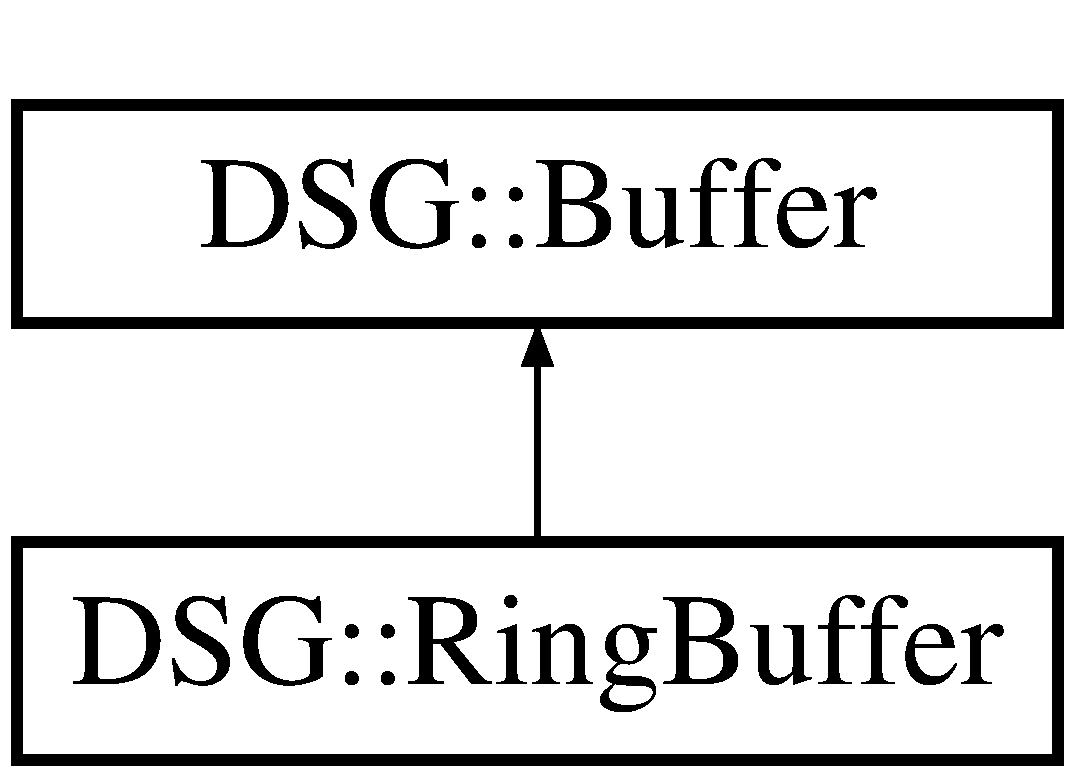
\includegraphics[height=2.000000cm]{classDSG_1_1RingBuffer}
\end{center}
\end{figure}
\subsection*{Public Member Functions}
\begin{DoxyCompactItemize}
\item 
\hyperlink{classDSG_1_1RingBuffer_a3136c9debb3c422adb1d5835e11b2b99}{Ring\+Buffer} ()
\item 
\hyperlink{classDSG_1_1RingBuffer_ae9859fd3ad18961de494d8b50fe4763e}{Ring\+Buffer} (const size\+\_\+t size)
\item 
\hyperlink{classDSG_1_1RingBuffer_ab09f32dacee49df3281c6701b7a4d737}{Ring\+Buffer} (\hyperlink{classDSG_1_1RingBuffer}{Ring\+Buffer} \&buffer)
\item 
\hyperlink{classDSG_1_1RingBuffer}{Ring\+Buffer} \& \hyperlink{classDSG_1_1RingBuffer_a892fbcc12b2dca5b04ead96a09299e73}{operator=} (\hyperlink{classDSG_1_1RingBuffer}{Ring\+Buffer} \&buffer)
\item 
virtual \hyperlink{classDSG_1_1RingBuffer_a771d30b04b6f0313c203530685fbeb3a}{$\sim$\+Ring\+Buffer} ()
\item 
bool \hyperlink{classDSG_1_1RingBuffer_af484c16dbffaf555860a84652ac46284}{Write} (const \hyperlink{classDSG_1_1Sample}{D\+S\+G\+::\+Sample} \&elem)
\item 
bool \hyperlink{classDSG_1_1RingBuffer_ae46649acd09c2e83834f3e31157b29b6}{Read} (\hyperlink{classDSG_1_1Sample}{D\+S\+G\+::\+Sample} \&elem)
\item 
size\+\_\+t const \& \hyperlink{classDSG_1_1RingBuffer_a9bd79b0a6dff618b205e396c101ee070}{Count} () const 
\item 
bool \hyperlink{classDSG_1_1RingBuffer_a53ddb04ffcbb5470a8d2b0a3c65b70cb}{Full} () const 
\item 
bool \hyperlink{classDSG_1_1RingBuffer_ac1346f5842d08b988a5297abe4089b96}{Empty} () const 
\item 
void \hyperlink{classDSG_1_1RingBuffer_ab23c8003d2857809a816068eeb209d60}{Flush} ()
\item 
\hyperlink{classDSG_1_1Sample}{Sample} \& \hyperlink{classDSG_1_1Buffer_a5dafe5522f3d20756f83e08499e8eaeb}{operator\mbox{[}$\,$\mbox{]}} (size\+\_\+t const \&index)
\item 
size\+\_\+t const \& \hyperlink{classDSG_1_1Buffer_a4acea659d9cd0be652ec55d21e5b0262}{Size} () const 
\end{DoxyCompactItemize}
\subsection*{Protected Member Functions}
\begin{DoxyCompactItemize}
\item 
size\+\_\+t \hyperlink{classDSG_1_1RingBuffer_a6d7a76a4c9b38ccde46344662e08c9e5}{next} (size\+\_\+t current)
\item 
size\+\_\+t \hyperlink{classDSG_1_1RingBuffer_aaf481e139011e91b111cc048e726cafb}{make\+\_\+pow\+\_\+2} (size\+\_\+t number)
\end{DoxyCompactItemize}
\subsection*{Protected Attributes}
\begin{DoxyCompactItemize}
\item 
std\+::atomic$<$ size\+\_\+t $>$ \hyperlink{classDSG_1_1RingBuffer_a78bd7704fd059b745bc82421e1062123}{\+\_\+write}
\item 
std\+::atomic$<$ size\+\_\+t $>$ \hyperlink{classDSG_1_1RingBuffer_aa71bb75a5d24700be795a30e1a135a54}{\+\_\+read}
\item 
size\+\_\+t \hyperlink{classDSG_1_1RingBuffer_af6d0e1658a1f1aa298218b890e458f2f}{\+\_\+count}
\item 
size\+\_\+t \hyperlink{classDSG_1_1RingBuffer_a2fba2ff6ee3886101f0f58b0fd7f3641}{M\+A\+S\+K}
\item 
size\+\_\+t \hyperlink{classDSG_1_1RingBuffer_a703434b6afb87f1f9a05750278a822e3}{write}
\item 
size\+\_\+t \hyperlink{classDSG_1_1RingBuffer_a34bc659c286c8913e318c0e8c0777204}{read}
\item 
\hyperlink{classDSG_1_1Sample}{Sample} $\ast$ \hyperlink{classDSG_1_1Buffer_a6506d4763401650acb463cb5d4913e31}{\+\_\+buffer}
\item 
size\+\_\+t \hyperlink{classDSG_1_1Buffer_a4e2fef9ed617af2554b25c999def8f71}{\+\_\+size}
\end{DoxyCompactItemize}


\subsection{Detailed Description}


Definition at line 24 of file Ring\+Buffer.\+h.



\subsection{Constructor \& Destructor Documentation}
\hypertarget{classDSG_1_1RingBuffer_a3136c9debb3c422adb1d5835e11b2b99}{\index{D\+S\+G\+::\+Ring\+Buffer@{D\+S\+G\+::\+Ring\+Buffer}!Ring\+Buffer@{Ring\+Buffer}}
\index{Ring\+Buffer@{Ring\+Buffer}!D\+S\+G\+::\+Ring\+Buffer@{D\+S\+G\+::\+Ring\+Buffer}}
\subsubsection[{Ring\+Buffer}]{\setlength{\rightskip}{0pt plus 5cm}D\+S\+G\+::\+Ring\+Buffer\+::\+Ring\+Buffer (
\begin{DoxyParamCaption}
{}
\end{DoxyParamCaption}
)}}\label{classDSG_1_1RingBuffer_a3136c9debb3c422adb1d5835e11b2b99}


Definition at line 14 of file Ring\+Buffer.\+cpp.


\begin{DoxyCode}
14 :\hyperlink{classDSG_1_1Buffer_aa764dd8c389dcff51de08cb81fafeb86}{Buffer}(0),\hyperlink{classDSG_1_1RingBuffer_aa71bb75a5d24700be795a30e1a135a54}{\_read}(0),\hyperlink{classDSG_1_1RingBuffer_a78bd7704fd059b745bc82421e1062123}{\_write}(0),\hyperlink{classDSG_1_1RingBuffer_af6d0e1658a1f1aa298218b890e458f2f}{\_count}(0),\hyperlink{classDSG_1_1RingBuffer_a2fba2ff6ee3886101f0f58b0fd7f3641}{MASK}(0)\{\}
\end{DoxyCode}
\hypertarget{classDSG_1_1RingBuffer_ae9859fd3ad18961de494d8b50fe4763e}{\index{D\+S\+G\+::\+Ring\+Buffer@{D\+S\+G\+::\+Ring\+Buffer}!Ring\+Buffer@{Ring\+Buffer}}
\index{Ring\+Buffer@{Ring\+Buffer}!D\+S\+G\+::\+Ring\+Buffer@{D\+S\+G\+::\+Ring\+Buffer}}
\subsubsection[{Ring\+Buffer}]{\setlength{\rightskip}{0pt plus 5cm}D\+S\+G\+::\+Ring\+Buffer\+::\+Ring\+Buffer (
\begin{DoxyParamCaption}
\item[{const size\+\_\+t}]{size}
\end{DoxyParamCaption}
)}}\label{classDSG_1_1RingBuffer_ae9859fd3ad18961de494d8b50fe4763e}


Definition at line 16 of file Ring\+Buffer.\+cpp.


\begin{DoxyCode}
16                                            :\hyperlink{classDSG_1_1Buffer_aa764dd8c389dcff51de08cb81fafeb86}{Buffer}(\hyperlink{classDSG_1_1RingBuffer_aaf481e139011e91b111cc048e726cafb}{make\_pow\_2}(size)),
      \hyperlink{classDSG_1_1RingBuffer_aa71bb75a5d24700be795a30e1a135a54}{\_read}(0),\hyperlink{classDSG_1_1RingBuffer_a78bd7704fd059b745bc82421e1062123}{\_write}(0),\hyperlink{classDSG_1_1RingBuffer_af6d0e1658a1f1aa298218b890e458f2f}{\_count}(0)\{
17     \hyperlink{classDSG_1_1RingBuffer_a2fba2ff6ee3886101f0f58b0fd7f3641}{MASK} = this->\hyperlink{classDSG_1_1Buffer_a4e2fef9ed617af2554b25c999def8f71}{\_size}-1;
18 \}
\end{DoxyCode}
\hypertarget{classDSG_1_1RingBuffer_ab09f32dacee49df3281c6701b7a4d737}{\index{D\+S\+G\+::\+Ring\+Buffer@{D\+S\+G\+::\+Ring\+Buffer}!Ring\+Buffer@{Ring\+Buffer}}
\index{Ring\+Buffer@{Ring\+Buffer}!D\+S\+G\+::\+Ring\+Buffer@{D\+S\+G\+::\+Ring\+Buffer}}
\subsubsection[{Ring\+Buffer}]{\setlength{\rightskip}{0pt plus 5cm}D\+S\+G\+::\+Ring\+Buffer\+::\+Ring\+Buffer (
\begin{DoxyParamCaption}
\item[{{\bf Ring\+Buffer} \&}]{buffer}
\end{DoxyParamCaption}
)}}\label{classDSG_1_1RingBuffer_ab09f32dacee49df3281c6701b7a4d737}


Definition at line 20 of file Ring\+Buffer.\+cpp.


\begin{DoxyCode}
20                                             :\hyperlink{classDSG_1_1Buffer_aa764dd8c389dcff51de08cb81fafeb86}{Buffer}(buffer)\{
21     \hyperlink{classDSG_1_1RingBuffer_a78bd7704fd059b745bc82421e1062123}{\_write}.store(buffer.\_write.load(std::memory\_order\_acquire));
22     \hyperlink{classDSG_1_1RingBuffer_aa71bb75a5d24700be795a30e1a135a54}{\_read}.store(buffer.\_read.load(std::memory\_order\_acquire));
23     \hyperlink{classDSG_1_1RingBuffer_af6d0e1658a1f1aa298218b890e458f2f}{\_count} = buffer.\_count;
24     \hyperlink{classDSG_1_1RingBuffer_a2fba2ff6ee3886101f0f58b0fd7f3641}{MASK} = buffer.\_size-1;
25 \}
\end{DoxyCode}
\hypertarget{classDSG_1_1RingBuffer_a771d30b04b6f0313c203530685fbeb3a}{\index{D\+S\+G\+::\+Ring\+Buffer@{D\+S\+G\+::\+Ring\+Buffer}!````~Ring\+Buffer@{$\sim$\+Ring\+Buffer}}
\index{````~Ring\+Buffer@{$\sim$\+Ring\+Buffer}!D\+S\+G\+::\+Ring\+Buffer@{D\+S\+G\+::\+Ring\+Buffer}}
\subsubsection[{$\sim$\+Ring\+Buffer}]{\setlength{\rightskip}{0pt plus 5cm}D\+S\+G\+::\+Ring\+Buffer\+::$\sim$\+Ring\+Buffer (
\begin{DoxyParamCaption}
{}
\end{DoxyParamCaption}
)\hspace{0.3cm}{\ttfamily [virtual]}}}\label{classDSG_1_1RingBuffer_a771d30b04b6f0313c203530685fbeb3a}


Definition at line 35 of file Ring\+Buffer.\+cpp.


\begin{DoxyCode}
35 \{\hyperlink{classDSG_1_1RingBuffer_ab23c8003d2857809a816068eeb209d60}{Flush}();\}
\end{DoxyCode}


\subsection{Member Function Documentation}
\hypertarget{classDSG_1_1RingBuffer_a9bd79b0a6dff618b205e396c101ee070}{\index{D\+S\+G\+::\+Ring\+Buffer@{D\+S\+G\+::\+Ring\+Buffer}!Count@{Count}}
\index{Count@{Count}!D\+S\+G\+::\+Ring\+Buffer@{D\+S\+G\+::\+Ring\+Buffer}}
\subsubsection[{Count}]{\setlength{\rightskip}{0pt plus 5cm}size\+\_\+t const \& D\+S\+G\+::\+Ring\+Buffer\+::\+Count (
\begin{DoxyParamCaption}
{}
\end{DoxyParamCaption}
) const\hspace{0.3cm}{\ttfamily [inline]}}}\label{classDSG_1_1RingBuffer_a9bd79b0a6dff618b205e396c101ee070}


Definition at line 82 of file Ring\+Buffer.\+h.


\begin{DoxyCode}
82                                                    \{
83             \textcolor{keywordflow}{return} \hyperlink{classDSG_1_1RingBuffer_af6d0e1658a1f1aa298218b890e458f2f}{\_count};
84         \}
\end{DoxyCode}
\hypertarget{classDSG_1_1RingBuffer_ac1346f5842d08b988a5297abe4089b96}{\index{D\+S\+G\+::\+Ring\+Buffer@{D\+S\+G\+::\+Ring\+Buffer}!Empty@{Empty}}
\index{Empty@{Empty}!D\+S\+G\+::\+Ring\+Buffer@{D\+S\+G\+::\+Ring\+Buffer}}
\subsubsection[{Empty}]{\setlength{\rightskip}{0pt plus 5cm}bool D\+S\+G\+::\+Ring\+Buffer\+::\+Empty (
\begin{DoxyParamCaption}
{}
\end{DoxyParamCaption}
) const\hspace{0.3cm}{\ttfamily [inline]}}}\label{classDSG_1_1RingBuffer_ac1346f5842d08b988a5297abe4089b96}


Definition at line 56 of file Ring\+Buffer.\+h.


\begin{DoxyCode}
56                                           \{
57             \textcolor{keywordflow}{return} \hyperlink{classDSG_1_1RingBuffer_af6d0e1658a1f1aa298218b890e458f2f}{\_count}==0;
58         \}
\end{DoxyCode}
\hypertarget{classDSG_1_1RingBuffer_ab23c8003d2857809a816068eeb209d60}{\index{D\+S\+G\+::\+Ring\+Buffer@{D\+S\+G\+::\+Ring\+Buffer}!Flush@{Flush}}
\index{Flush@{Flush}!D\+S\+G\+::\+Ring\+Buffer@{D\+S\+G\+::\+Ring\+Buffer}}
\subsubsection[{Flush}]{\setlength{\rightskip}{0pt plus 5cm}void D\+S\+G\+::\+Ring\+Buffer\+::\+Flush (
\begin{DoxyParamCaption}
{}
\end{DoxyParamCaption}
)\hspace{0.3cm}{\ttfamily [inline]}}}\label{classDSG_1_1RingBuffer_ab23c8003d2857809a816068eeb209d60}


Definition at line 59 of file Ring\+Buffer.\+h.


\begin{DoxyCode}
59                                      \{
60             \hyperlink{classDSG_1_1RingBuffer_a78bd7704fd059b745bc82421e1062123}{\_write}.store(0,std::memory\_order\_relaxed);
61             \hyperlink{classDSG_1_1RingBuffer_aa71bb75a5d24700be795a30e1a135a54}{\_read}.store(0,std::memory\_order\_relaxed);
62             \hyperlink{classDSG_1_1RingBuffer_af6d0e1658a1f1aa298218b890e458f2f}{\_count}=0;
63         \}
\end{DoxyCode}
\hypertarget{classDSG_1_1RingBuffer_a53ddb04ffcbb5470a8d2b0a3c65b70cb}{\index{D\+S\+G\+::\+Ring\+Buffer@{D\+S\+G\+::\+Ring\+Buffer}!Full@{Full}}
\index{Full@{Full}!D\+S\+G\+::\+Ring\+Buffer@{D\+S\+G\+::\+Ring\+Buffer}}
\subsubsection[{Full}]{\setlength{\rightskip}{0pt plus 5cm}bool D\+S\+G\+::\+Ring\+Buffer\+::\+Full (
\begin{DoxyParamCaption}
{}
\end{DoxyParamCaption}
) const\hspace{0.3cm}{\ttfamily [inline]}}}\label{classDSG_1_1RingBuffer_a53ddb04ffcbb5470a8d2b0a3c65b70cb}


Definition at line 53 of file Ring\+Buffer.\+h.


\begin{DoxyCode}
53                                          \{
54             \textcolor{keywordflow}{return} \hyperlink{classDSG_1_1RingBuffer_af6d0e1658a1f1aa298218b890e458f2f}{\_count}==this->\hyperlink{classDSG_1_1Buffer_a4e2fef9ed617af2554b25c999def8f71}{\_size};
55         \}
\end{DoxyCode}
\hypertarget{classDSG_1_1RingBuffer_aaf481e139011e91b111cc048e726cafb}{\index{D\+S\+G\+::\+Ring\+Buffer@{D\+S\+G\+::\+Ring\+Buffer}!make\+\_\+pow\+\_\+2@{make\+\_\+pow\+\_\+2}}
\index{make\+\_\+pow\+\_\+2@{make\+\_\+pow\+\_\+2}!D\+S\+G\+::\+Ring\+Buffer@{D\+S\+G\+::\+Ring\+Buffer}}
\subsubsection[{make\+\_\+pow\+\_\+2}]{\setlength{\rightskip}{0pt plus 5cm}size\+\_\+t D\+S\+G\+::\+Ring\+Buffer\+::make\+\_\+pow\+\_\+2 (
\begin{DoxyParamCaption}
\item[{size\+\_\+t}]{number}
\end{DoxyParamCaption}
)\hspace{0.3cm}{\ttfamily [inline]}, {\ttfamily [protected]}}}\label{classDSG_1_1RingBuffer_aaf481e139011e91b111cc048e726cafb}


Definition at line 88 of file Ring\+Buffer.\+h.


\begin{DoxyCode}
88                                                          \{
89             \textcolor{keywordflow}{return} pow(2, ceil(log(number)/log(2)));
90         \}
\end{DoxyCode}
\hypertarget{classDSG_1_1RingBuffer_a6d7a76a4c9b38ccde46344662e08c9e5}{\index{D\+S\+G\+::\+Ring\+Buffer@{D\+S\+G\+::\+Ring\+Buffer}!next@{next}}
\index{next@{next}!D\+S\+G\+::\+Ring\+Buffer@{D\+S\+G\+::\+Ring\+Buffer}}
\subsubsection[{next}]{\setlength{\rightskip}{0pt plus 5cm}size\+\_\+t D\+S\+G\+::\+Ring\+Buffer\+::next (
\begin{DoxyParamCaption}
\item[{size\+\_\+t}]{current}
\end{DoxyParamCaption}
)\hspace{0.3cm}{\ttfamily [inline]}, {\ttfamily [protected]}}}\label{classDSG_1_1RingBuffer_a6d7a76a4c9b38ccde46344662e08c9e5}


Definition at line 87 of file Ring\+Buffer.\+h.


\begin{DoxyCode}
87 \{\textcolor{keywordflow}{return} (current+1) & \hyperlink{classDSG_1_1RingBuffer_a2fba2ff6ee3886101f0f58b0fd7f3641}{MASK};\}
\end{DoxyCode}
\hypertarget{classDSG_1_1RingBuffer_a892fbcc12b2dca5b04ead96a09299e73}{\index{D\+S\+G\+::\+Ring\+Buffer@{D\+S\+G\+::\+Ring\+Buffer}!operator=@{operator=}}
\index{operator=@{operator=}!D\+S\+G\+::\+Ring\+Buffer@{D\+S\+G\+::\+Ring\+Buffer}}
\subsubsection[{operator=}]{\setlength{\rightskip}{0pt plus 5cm}{\bf D\+S\+G\+::\+Ring\+Buffer} \& D\+S\+G\+::\+Ring\+Buffer\+::operator= (
\begin{DoxyParamCaption}
\item[{{\bf Ring\+Buffer} \&}]{buffer}
\end{DoxyParamCaption}
)}}\label{classDSG_1_1RingBuffer_a892fbcc12b2dca5b04ead96a09299e73}


Definition at line 27 of file Ring\+Buffer.\+cpp.


\begin{DoxyCode}
27                                                            \{
28     \hyperlink{classDSG_1_1Buffer_a977d572a7d402ff6bf991d7c5c0cc6a7}{Buffer::operator=}(buffer);
29     \hyperlink{classDSG_1_1RingBuffer_a78bd7704fd059b745bc82421e1062123}{\_write}.store(buffer.\_write.load(std::memory\_order\_acquire));
30     \hyperlink{classDSG_1_1RingBuffer_aa71bb75a5d24700be795a30e1a135a54}{\_read}.store(buffer.\_read.load(std::memory\_order\_acquire));
31     \hyperlink{classDSG_1_1RingBuffer_af6d0e1658a1f1aa298218b890e458f2f}{\_count} = buffer.\_count;
32     \hyperlink{classDSG_1_1RingBuffer_a2fba2ff6ee3886101f0f58b0fd7f3641}{MASK} = buffer.\_size-1;
33     \textcolor{keywordflow}{return} *\textcolor{keyword}{this};
34 \}
\end{DoxyCode}
\hypertarget{classDSG_1_1Buffer_a5dafe5522f3d20756f83e08499e8eaeb}{\index{D\+S\+G\+::\+Ring\+Buffer@{D\+S\+G\+::\+Ring\+Buffer}!operator\mbox{[}$\,$\mbox{]}@{operator[]}}
\index{operator\mbox{[}$\,$\mbox{]}@{operator[]}!D\+S\+G\+::\+Ring\+Buffer@{D\+S\+G\+::\+Ring\+Buffer}}
\subsubsection[{operator[]}]{\setlength{\rightskip}{0pt plus 5cm}{\bf D\+S\+G\+::\+Sample} \& D\+S\+G\+::\+Buffer\+::operator\mbox{[}$\,$\mbox{]} (
\begin{DoxyParamCaption}
\item[{size\+\_\+t const \&}]{index}
\end{DoxyParamCaption}
)\hspace{0.3cm}{\ttfamily [inherited]}}}\label{classDSG_1_1Buffer_a5dafe5522f3d20756f83e08499e8eaeb}


Definition at line 38 of file Buffer.\+cpp.


\begin{DoxyCode}
38                                                     \{
39 \textcolor{preprocessor}{#ifdef DEBUG}
40     assert(index<\hyperlink{classDSG_1_1Buffer_a4e2fef9ed617af2554b25c999def8f71}{\_size});
41 \textcolor{preprocessor}{#endif}
42     \textcolor{keywordflow}{return} \hyperlink{classDSG_1_1Buffer_a6506d4763401650acb463cb5d4913e31}{\_buffer}[index];
43 \}
\end{DoxyCode}
\hypertarget{classDSG_1_1RingBuffer_ae46649acd09c2e83834f3e31157b29b6}{\index{D\+S\+G\+::\+Ring\+Buffer@{D\+S\+G\+::\+Ring\+Buffer}!Read@{Read}}
\index{Read@{Read}!D\+S\+G\+::\+Ring\+Buffer@{D\+S\+G\+::\+Ring\+Buffer}}
\subsubsection[{Read}]{\setlength{\rightskip}{0pt plus 5cm}bool D\+S\+G\+::\+Ring\+Buffer\+::\+Read (
\begin{DoxyParamCaption}
\item[{{\bf D\+S\+G\+::\+Sample} \&}]{elem}
\end{DoxyParamCaption}
)\hspace{0.3cm}{\ttfamily [inline]}}}\label{classDSG_1_1RingBuffer_ae46649acd09c2e83834f3e31157b29b6}


Definition at line 73 of file Ring\+Buffer.\+h.


\begin{DoxyCode}
73                                                 \{
74             \textcolor{keywordflow}{if} (!\hyperlink{classDSG_1_1RingBuffer_ac1346f5842d08b988a5297abe4089b96}{Empty}()) \{
75                 \hyperlink{classDSG_1_1RingBuffer_a34bc659c286c8913e318c0e8c0777204}{read} = \hyperlink{classDSG_1_1RingBuffer_aa71bb75a5d24700be795a30e1a135a54}{\_read}.load(std::memory\_order\_acquire);
76                 \hyperlink{classDSG_1_1RingBuffer_aa71bb75a5d24700be795a30e1a135a54}{\_read}.store(\hyperlink{classDSG_1_1RingBuffer_a6d7a76a4c9b38ccde46344662e08c9e5}{next}(\hyperlink{classDSG_1_1RingBuffer_a34bc659c286c8913e318c0e8c0777204}{read}),std::memory\_order\_release);
77                 elem = this->\hyperlink{classDSG_1_1Buffer_a6506d4763401650acb463cb5d4913e31}{\_buffer}[\hyperlink{classDSG_1_1RingBuffer_a34bc659c286c8913e318c0e8c0777204}{read}];
78                 --\hyperlink{classDSG_1_1RingBuffer_af6d0e1658a1f1aa298218b890e458f2f}{\_count};
79                 \textcolor{keywordflow}{return} \textcolor{keyword}{true};
80             \}\textcolor{keywordflow}{else} \textcolor{keywordflow}{return} \textcolor{keyword}{false};
81         \}
\end{DoxyCode}
\hypertarget{classDSG_1_1Buffer_a4acea659d9cd0be652ec55d21e5b0262}{\index{D\+S\+G\+::\+Ring\+Buffer@{D\+S\+G\+::\+Ring\+Buffer}!Size@{Size}}
\index{Size@{Size}!D\+S\+G\+::\+Ring\+Buffer@{D\+S\+G\+::\+Ring\+Buffer}}
\subsubsection[{Size}]{\setlength{\rightskip}{0pt plus 5cm}size\+\_\+t const \& D\+S\+G\+::\+Buffer\+::\+Size (
\begin{DoxyParamCaption}
{}
\end{DoxyParamCaption}
) const\hspace{0.3cm}{\ttfamily [inline]}, {\ttfamily [inherited]}}}\label{classDSG_1_1Buffer_a4acea659d9cd0be652ec55d21e5b0262}


Definition at line 31 of file Buffer.\+h.


\begin{DoxyCode}
31                                           \{
32         \textcolor{keywordflow}{return} \hyperlink{classDSG_1_1Buffer_a4e2fef9ed617af2554b25c999def8f71}{\_size};
33     \}
\end{DoxyCode}
\hypertarget{classDSG_1_1RingBuffer_af484c16dbffaf555860a84652ac46284}{\index{D\+S\+G\+::\+Ring\+Buffer@{D\+S\+G\+::\+Ring\+Buffer}!Write@{Write}}
\index{Write@{Write}!D\+S\+G\+::\+Ring\+Buffer@{D\+S\+G\+::\+Ring\+Buffer}}
\subsubsection[{Write}]{\setlength{\rightskip}{0pt plus 5cm}bool D\+S\+G\+::\+Ring\+Buffer\+::\+Write (
\begin{DoxyParamCaption}
\item[{const {\bf D\+S\+G\+::\+Sample} \&}]{elem}
\end{DoxyParamCaption}
)\hspace{0.3cm}{\ttfamily [inline]}}}\label{classDSG_1_1RingBuffer_af484c16dbffaf555860a84652ac46284}


Definition at line 64 of file Ring\+Buffer.\+h.


\begin{DoxyCode}
64                                                        \{
65             \textcolor{keywordflow}{if} (!\hyperlink{classDSG_1_1RingBuffer_a53ddb04ffcbb5470a8d2b0a3c65b70cb}{Full}()) \{
66                 \hyperlink{classDSG_1_1RingBuffer_a703434b6afb87f1f9a05750278a822e3}{write} = \hyperlink{classDSG_1_1RingBuffer_a78bd7704fd059b745bc82421e1062123}{\_write}.load(std::memory\_order\_acquire);
67                 \hyperlink{classDSG_1_1RingBuffer_a78bd7704fd059b745bc82421e1062123}{\_write}.store(\hyperlink{classDSG_1_1RingBuffer_a6d7a76a4c9b38ccde46344662e08c9e5}{next}(\hyperlink{classDSG_1_1RingBuffer_a703434b6afb87f1f9a05750278a822e3}{write}),std::memory\_order\_release);
68                 this->\hyperlink{classDSG_1_1Buffer_a6506d4763401650acb463cb5d4913e31}{\_buffer}[\hyperlink{classDSG_1_1RingBuffer_a703434b6afb87f1f9a05750278a822e3}{write}] = elem;
69                 ++\hyperlink{classDSG_1_1RingBuffer_af6d0e1658a1f1aa298218b890e458f2f}{\_count};
70                 \textcolor{keywordflow}{return} \textcolor{keyword}{true};
71             \}\textcolor{keywordflow}{else} \textcolor{keywordflow}{return} \textcolor{keyword}{false};
72         \}
\end{DoxyCode}


\subsection{Member Data Documentation}
\hypertarget{classDSG_1_1Buffer_a6506d4763401650acb463cb5d4913e31}{\index{D\+S\+G\+::\+Ring\+Buffer@{D\+S\+G\+::\+Ring\+Buffer}!\+\_\+buffer@{\+\_\+buffer}}
\index{\+\_\+buffer@{\+\_\+buffer}!D\+S\+G\+::\+Ring\+Buffer@{D\+S\+G\+::\+Ring\+Buffer}}
\subsubsection[{\+\_\+buffer}]{\setlength{\rightskip}{0pt plus 5cm}{\bf Sample}$\ast$ D\+S\+G\+::\+Buffer\+::\+\_\+buffer\hspace{0.3cm}{\ttfamily [protected]}, {\ttfamily [inherited]}}}\label{classDSG_1_1Buffer_a6506d4763401650acb463cb5d4913e31}


Definition at line 28 of file Buffer.\+h.

\hypertarget{classDSG_1_1RingBuffer_af6d0e1658a1f1aa298218b890e458f2f}{\index{D\+S\+G\+::\+Ring\+Buffer@{D\+S\+G\+::\+Ring\+Buffer}!\+\_\+count@{\+\_\+count}}
\index{\+\_\+count@{\+\_\+count}!D\+S\+G\+::\+Ring\+Buffer@{D\+S\+G\+::\+Ring\+Buffer}}
\subsubsection[{\+\_\+count}]{\setlength{\rightskip}{0pt plus 5cm}size\+\_\+t D\+S\+G\+::\+Ring\+Buffer\+::\+\_\+count\hspace{0.3cm}{\ttfamily [protected]}}}\label{classDSG_1_1RingBuffer_af6d0e1658a1f1aa298218b890e458f2f}


Definition at line 28 of file Ring\+Buffer.\+h.

\hypertarget{classDSG_1_1RingBuffer_aa71bb75a5d24700be795a30e1a135a54}{\index{D\+S\+G\+::\+Ring\+Buffer@{D\+S\+G\+::\+Ring\+Buffer}!\+\_\+read@{\+\_\+read}}
\index{\+\_\+read@{\+\_\+read}!D\+S\+G\+::\+Ring\+Buffer@{D\+S\+G\+::\+Ring\+Buffer}}
\subsubsection[{\+\_\+read}]{\setlength{\rightskip}{0pt plus 5cm}std\+::atomic$<$size\+\_\+t$>$ D\+S\+G\+::\+Ring\+Buffer\+::\+\_\+read\hspace{0.3cm}{\ttfamily [protected]}}}\label{classDSG_1_1RingBuffer_aa71bb75a5d24700be795a30e1a135a54}


Definition at line 27 of file Ring\+Buffer.\+h.

\hypertarget{classDSG_1_1Buffer_a4e2fef9ed617af2554b25c999def8f71}{\index{D\+S\+G\+::\+Ring\+Buffer@{D\+S\+G\+::\+Ring\+Buffer}!\+\_\+size@{\+\_\+size}}
\index{\+\_\+size@{\+\_\+size}!D\+S\+G\+::\+Ring\+Buffer@{D\+S\+G\+::\+Ring\+Buffer}}
\subsubsection[{\+\_\+size}]{\setlength{\rightskip}{0pt plus 5cm}size\+\_\+t D\+S\+G\+::\+Buffer\+::\+\_\+size\hspace{0.3cm}{\ttfamily [protected]}, {\ttfamily [inherited]}}}\label{classDSG_1_1Buffer_a4e2fef9ed617af2554b25c999def8f71}


Definition at line 29 of file Buffer.\+h.

\hypertarget{classDSG_1_1RingBuffer_a78bd7704fd059b745bc82421e1062123}{\index{D\+S\+G\+::\+Ring\+Buffer@{D\+S\+G\+::\+Ring\+Buffer}!\+\_\+write@{\+\_\+write}}
\index{\+\_\+write@{\+\_\+write}!D\+S\+G\+::\+Ring\+Buffer@{D\+S\+G\+::\+Ring\+Buffer}}
\subsubsection[{\+\_\+write}]{\setlength{\rightskip}{0pt plus 5cm}std\+::atomic$<$size\+\_\+t$>$ D\+S\+G\+::\+Ring\+Buffer\+::\+\_\+write\hspace{0.3cm}{\ttfamily [protected]}}}\label{classDSG_1_1RingBuffer_a78bd7704fd059b745bc82421e1062123}


Definition at line 26 of file Ring\+Buffer.\+h.

\hypertarget{classDSG_1_1RingBuffer_a2fba2ff6ee3886101f0f58b0fd7f3641}{\index{D\+S\+G\+::\+Ring\+Buffer@{D\+S\+G\+::\+Ring\+Buffer}!M\+A\+S\+K@{M\+A\+S\+K}}
\index{M\+A\+S\+K@{M\+A\+S\+K}!D\+S\+G\+::\+Ring\+Buffer@{D\+S\+G\+::\+Ring\+Buffer}}
\subsubsection[{M\+A\+S\+K}]{\setlength{\rightskip}{0pt plus 5cm}size\+\_\+t D\+S\+G\+::\+Ring\+Buffer\+::\+M\+A\+S\+K\hspace{0.3cm}{\ttfamily [protected]}}}\label{classDSG_1_1RingBuffer_a2fba2ff6ee3886101f0f58b0fd7f3641}


Definition at line 29 of file Ring\+Buffer.\+h.

\hypertarget{classDSG_1_1RingBuffer_a34bc659c286c8913e318c0e8c0777204}{\index{D\+S\+G\+::\+Ring\+Buffer@{D\+S\+G\+::\+Ring\+Buffer}!read@{read}}
\index{read@{read}!D\+S\+G\+::\+Ring\+Buffer@{D\+S\+G\+::\+Ring\+Buffer}}
\subsubsection[{read}]{\setlength{\rightskip}{0pt plus 5cm}size\+\_\+t D\+S\+G\+::\+Ring\+Buffer\+::read\hspace{0.3cm}{\ttfamily [protected]}}}\label{classDSG_1_1RingBuffer_a34bc659c286c8913e318c0e8c0777204}


Definition at line 32 of file Ring\+Buffer.\+h.

\hypertarget{classDSG_1_1RingBuffer_a703434b6afb87f1f9a05750278a822e3}{\index{D\+S\+G\+::\+Ring\+Buffer@{D\+S\+G\+::\+Ring\+Buffer}!write@{write}}
\index{write@{write}!D\+S\+G\+::\+Ring\+Buffer@{D\+S\+G\+::\+Ring\+Buffer}}
\subsubsection[{write}]{\setlength{\rightskip}{0pt plus 5cm}size\+\_\+t D\+S\+G\+::\+Ring\+Buffer\+::write\hspace{0.3cm}{\ttfamily [protected]}}}\label{classDSG_1_1RingBuffer_a703434b6afb87f1f9a05750278a822e3}


Definition at line 31 of file Ring\+Buffer.\+h.



The documentation for this class was generated from the following files\+:\begin{DoxyCompactItemize}
\item 
/\+Users/alexanderzywicki/\+Documents/\+School\+\_\+\+Stuff/\+Fall\+\_\+2014/\+Digital\+\_\+\+Signal\+\_\+\+Generation\+\_\+and\+\_\+\+Analysis/src/include/\hyperlink{RingBuffer_8h}{Ring\+Buffer.\+h}\item 
/\+Users/alexanderzywicki/\+Documents/\+School\+\_\+\+Stuff/\+Fall\+\_\+2014/\+Digital\+\_\+\+Signal\+\_\+\+Generation\+\_\+and\+\_\+\+Analysis/src/\hyperlink{RingBuffer_8cpp}{Ring\+Buffer.\+cpp}\end{DoxyCompactItemize}

\hypertarget{classDSG_1_1Sample}{\section{D\+S\+G\+:\+:Sample Class Reference}
\label{classDSG_1_1Sample}\index{D\+S\+G\+::\+Sample@{D\+S\+G\+::\+Sample}}
}


Stereo Audio \hyperlink{classDSG_1_1Sample}{Sample} Class.  




{\ttfamily \#include $<$Sample.\+h$>$}

\subsection*{Public Member Functions}
\begin{DoxyCompactItemize}
\item 
\hyperlink{classDSG_1_1Sample_aaf2e30d73911eccea99b53eeee15b612}{Sample} ()
\item 
\hyperlink{classDSG_1_1Sample_a9b5f59392d91826ceceec0481f677264}{Sample} (float value)
\item 
\hyperlink{classDSG_1_1Sample_a97befdd6c269432bbba374cdb51e3241}{Sample} (float c0, float c1)
\item 
\hyperlink{classDSG_1_1Sample_a4d5a42f2264c88291e49df89588dee50}{Sample} (\hyperlink{classDSG_1_1Sample}{Sample} const \&samp)
\item 
\hyperlink{classDSG_1_1Sample}{Sample} \& \hyperlink{classDSG_1_1Sample_a55248a848f30a533d51e6d0da2d4a3e2}{operator=} (\hyperlink{classDSG_1_1Sample}{Sample} const \&samp)
\item 
\hyperlink{classDSG_1_1Sample_af5a24cf30417259e03b5176cd2aadd0c}{$\sim$\+Sample} ()
\item 
size\+\_\+t \hyperlink{classDSG_1_1Sample_abcbdcc67584e4018b24eac650724eb18}{Size} () const 
\item 
float \& \hyperlink{classDSG_1_1Sample_ac0f49c86a2b59e15ba761ec308560828}{operator\mbox{[}$\,$\mbox{]}} (const size\+\_\+t \&index)
\item 
float const \& \hyperlink{classDSG_1_1Sample_a5908819bba1cd5110593ad3f66154b53}{operator\mbox{[}$\,$\mbox{]}} (const size\+\_\+t \&index) const 
\item 
\hyperlink{classDSG_1_1Sample}{Sample} \& \hyperlink{classDSG_1_1Sample_a8eb7f791c233ade5218bc4186e390c2e}{operator=} (float const \&value)
\item 
\hyperlink{classDSG_1_1Sample}{Sample} \& \hyperlink{classDSG_1_1Sample_a608fc9b6936c9695e35c39b33623f0d9}{operator+=} (\hyperlink{classDSG_1_1Sample}{Sample} const \&samp)
\item 
\hyperlink{classDSG_1_1Sample}{Sample} \& \hyperlink{classDSG_1_1Sample_aa1467c3ac617c8920131be21be90c55e}{operator+=} (const float \&samp)
\item 
\hyperlink{classDSG_1_1Sample}{Sample} \& \hyperlink{classDSG_1_1Sample_a3e8c9bfb07c9a1abfbb925e943a77bf2}{operator-\/=} (\hyperlink{classDSG_1_1Sample}{Sample} const \&samp)
\item 
\hyperlink{classDSG_1_1Sample}{Sample} \& \hyperlink{classDSG_1_1Sample_a5c51de986eb773feaa20f3d7408f61fc}{operator-\/=} (const float \&samp)
\item 
\hyperlink{classDSG_1_1Sample}{Sample} \& \hyperlink{classDSG_1_1Sample_acfa0e39c59c941feda43cbf2163d3a3f}{operator$\ast$=} (\hyperlink{classDSG_1_1Sample}{Sample} const \&samp)
\item 
\hyperlink{classDSG_1_1Sample}{Sample} \& \hyperlink{classDSG_1_1Sample_ac7b0d51f729b74652eb942cac16231be}{operator$\ast$=} (const float \&samp)
\item 
\hyperlink{classDSG_1_1Sample}{Sample} \& \hyperlink{classDSG_1_1Sample_a426f95e1ca00e31f597e7974aa348fea}{operator/=} (\hyperlink{classDSG_1_1Sample}{Sample} const \&samp)
\item 
\hyperlink{classDSG_1_1Sample}{Sample} \& \hyperlink{classDSG_1_1Sample_a4949b575aa87fbe23d1f94ebc59a39ad}{operator/=} (const float \&samp)
\item 
\hyperlink{classDSG_1_1Sample}{Sample} \& \hyperlink{classDSG_1_1Sample_ac208ffaa812c14088a87d808048e5901}{operator++} ()
\item 
\hyperlink{classDSG_1_1Sample}{Sample} \hyperlink{classDSG_1_1Sample_a8a46b665400a64135dfa47626775a768}{operator++} (int)
\item 
\hyperlink{classDSG_1_1Sample}{Sample} \& \hyperlink{classDSG_1_1Sample_a592fa599991ca50854a43e6bdbe11ac5}{operator-\/-\/} ()
\item 
\hyperlink{classDSG_1_1Sample}{Sample} \hyperlink{classDSG_1_1Sample_a515bd70b0ad0a894bc279bc772ca4053}{operator-\/-\/} (int)
\item 
bool \hyperlink{classDSG_1_1Sample_a60ee416ba78328059219bf9ef2f716d8}{operator==} (\hyperlink{classDSG_1_1Sample}{Sample} \&samp)
\item 
bool \hyperlink{classDSG_1_1Sample_aaea02c560205ffe02fc0c2dda296f3f8}{operator!=} (\hyperlink{classDSG_1_1Sample}{Sample} \&samp)
\end{DoxyCompactItemize}
\subsection*{Protected Attributes}
\begin{DoxyCompactItemize}
\item 
float \hyperlink{classDSG_1_1Sample_ab3b67b009491583e03d8e97d579e67c2}{\+\_\+buffer} \mbox{[}\hyperlink{Sample_8h_a29e42927003b0aa647ee45965f4ccb07}{C\+H\+A\+N\+N\+E\+L\+\_\+\+C\+O\+U\+N\+T}\mbox{]}
\end{DoxyCompactItemize}
\subsection*{Friends}
\begin{DoxyCompactItemize}
\item 
\hyperlink{classDSG_1_1Sample}{Sample} \hyperlink{classDSG_1_1Sample_a2fd9547bca678d483b7678ff2d19c7bf}{operator+} (\hyperlink{classDSG_1_1Sample}{Sample} const \&s1, \hyperlink{classDSG_1_1Sample}{Sample} const \&s2)
\item 
\hyperlink{classDSG_1_1Sample}{Sample} \hyperlink{classDSG_1_1Sample_a001ec49a9676fe37d9dfbb6f0b27127d}{operator+} (\hyperlink{classDSG_1_1Sample}{Sample} const \&samp, float val)
\item 
\hyperlink{classDSG_1_1Sample}{Sample} \hyperlink{classDSG_1_1Sample_a9a5ae50b9096d1c778d6a676b562e11a}{operator+} (float val, \hyperlink{classDSG_1_1Sample}{Sample} const \&samp)
\item 
\hyperlink{classDSG_1_1Sample}{Sample} \hyperlink{classDSG_1_1Sample_a4539e34cec889979677229c5ddf6eaf1}{operator-\/} (\hyperlink{classDSG_1_1Sample}{Sample} const \&s1, \hyperlink{classDSG_1_1Sample}{Sample} const \&s2)
\item 
\hyperlink{classDSG_1_1Sample}{Sample} \hyperlink{classDSG_1_1Sample_a30c04ca57e9f947cdd68041231676acc}{operator-\/} (\hyperlink{classDSG_1_1Sample}{Sample} const \&samp, float val)
\item 
\hyperlink{classDSG_1_1Sample}{Sample} \hyperlink{classDSG_1_1Sample_a27b97bc41eae03efe5f4157bdc3e42b2}{operator-\/} (float val, \hyperlink{classDSG_1_1Sample}{Sample} const \&samp)
\item 
\hyperlink{classDSG_1_1Sample}{Sample} \hyperlink{classDSG_1_1Sample_ae6e21a0672b773c8ae0537410c48a385}{operator$\ast$} (\hyperlink{classDSG_1_1Sample}{Sample} const \&s1, \hyperlink{classDSG_1_1Sample}{Sample} const \&s2)
\item 
\hyperlink{classDSG_1_1Sample}{Sample} \hyperlink{classDSG_1_1Sample_a6c56eccda9469f7283e67c6e89b05239}{operator$\ast$} (\hyperlink{classDSG_1_1Sample}{Sample} const \&samp, float val)
\item 
\hyperlink{classDSG_1_1Sample}{Sample} \hyperlink{classDSG_1_1Sample_afacc0c2623435bca02ee4049ed2db550}{operator$\ast$} (float val, \hyperlink{classDSG_1_1Sample}{Sample} const \&samp)
\item 
\hyperlink{classDSG_1_1Sample}{Sample} \hyperlink{classDSG_1_1Sample_a26dc248966f0cb3c5d1c52f7aa6643d4}{operator/} (\hyperlink{classDSG_1_1Sample}{Sample} const \&s1, \hyperlink{classDSG_1_1Sample}{Sample} const \&s2)
\item 
\hyperlink{classDSG_1_1Sample}{Sample} \hyperlink{classDSG_1_1Sample_a135d15a9237414aabce1df8f3a5ae77f}{operator/} (\hyperlink{classDSG_1_1Sample}{Sample} const \&samp, float val)
\item 
\hyperlink{classDSG_1_1Sample}{Sample} \hyperlink{classDSG_1_1Sample_a6178925f7213e13df7f4106cc0e22330}{operator/} (float val, \hyperlink{classDSG_1_1Sample}{Sample} const \&samp)
\end{DoxyCompactItemize}


\subsection{Detailed Description}
Stereo Audio \hyperlink{classDSG_1_1Sample}{Sample} Class. 

Definition at line 20 of file Sample.\+h.



\subsection{Constructor \& Destructor Documentation}
\hypertarget{classDSG_1_1Sample_aaf2e30d73911eccea99b53eeee15b612}{\index{D\+S\+G\+::\+Sample@{D\+S\+G\+::\+Sample}!Sample@{Sample}}
\index{Sample@{Sample}!D\+S\+G\+::\+Sample@{D\+S\+G\+::\+Sample}}
\subsubsection[{Sample}]{\setlength{\rightskip}{0pt plus 5cm}D\+S\+G\+::\+Sample\+::\+Sample (
\begin{DoxyParamCaption}
{}
\end{DoxyParamCaption}
)}}\label{classDSG_1_1Sample_aaf2e30d73911eccea99b53eeee15b612}


Definition at line 9 of file Sample.\+cpp.


\begin{DoxyCode}
9                   \{
10     \hyperlink{classDSG_1_1Sample_ab3b67b009491583e03d8e97d579e67c2}{\_buffer}[0]=0;
11     \hyperlink{classDSG_1_1Sample_ab3b67b009491583e03d8e97d579e67c2}{\_buffer}[1]=0;
12 \}
\end{DoxyCode}
\hypertarget{classDSG_1_1Sample_a9b5f59392d91826ceceec0481f677264}{\index{D\+S\+G\+::\+Sample@{D\+S\+G\+::\+Sample}!Sample@{Sample}}
\index{Sample@{Sample}!D\+S\+G\+::\+Sample@{D\+S\+G\+::\+Sample}}
\subsubsection[{Sample}]{\setlength{\rightskip}{0pt plus 5cm}D\+S\+G\+::\+Sample\+::\+Sample (
\begin{DoxyParamCaption}
\item[{float}]{value}
\end{DoxyParamCaption}
)}}\label{classDSG_1_1Sample_a9b5f59392d91826ceceec0481f677264}


Definition at line 13 of file Sample.\+cpp.


\begin{DoxyCode}
13                              \{
14     *\textcolor{keyword}{this} = value;
15 \}
\end{DoxyCode}
\hypertarget{classDSG_1_1Sample_a97befdd6c269432bbba374cdb51e3241}{\index{D\+S\+G\+::\+Sample@{D\+S\+G\+::\+Sample}!Sample@{Sample}}
\index{Sample@{Sample}!D\+S\+G\+::\+Sample@{D\+S\+G\+::\+Sample}}
\subsubsection[{Sample}]{\setlength{\rightskip}{0pt plus 5cm}D\+S\+G\+::\+Sample\+::\+Sample (
\begin{DoxyParamCaption}
\item[{float}]{c0, }
\item[{float}]{c1}
\end{DoxyParamCaption}
)}}\label{classDSG_1_1Sample_a97befdd6c269432bbba374cdb51e3241}


Definition at line 16 of file Sample.\+cpp.


\begin{DoxyCode}
16                                    \{
17     \hyperlink{classDSG_1_1Sample_ab3b67b009491583e03d8e97d579e67c2}{\_buffer}[0]=c0;
18     \hyperlink{classDSG_1_1Sample_ab3b67b009491583e03d8e97d579e67c2}{\_buffer}[1]=c1;
19 \}
\end{DoxyCode}
\hypertarget{classDSG_1_1Sample_a4d5a42f2264c88291e49df89588dee50}{\index{D\+S\+G\+::\+Sample@{D\+S\+G\+::\+Sample}!Sample@{Sample}}
\index{Sample@{Sample}!D\+S\+G\+::\+Sample@{D\+S\+G\+::\+Sample}}
\subsubsection[{Sample}]{\setlength{\rightskip}{0pt plus 5cm}D\+S\+G\+::\+Sample\+::\+Sample (
\begin{DoxyParamCaption}
\item[{{\bf D\+S\+G\+::\+Sample} const \&}]{samp}
\end{DoxyParamCaption}
)}}\label{classDSG_1_1Sample_a4d5a42f2264c88291e49df89588dee50}


Definition at line 20 of file Sample.\+cpp.


\begin{DoxyCode}
20                                         \{
21     *\textcolor{keyword}{this} = samp;
22 \}
\end{DoxyCode}
\hypertarget{classDSG_1_1Sample_af5a24cf30417259e03b5176cd2aadd0c}{\index{D\+S\+G\+::\+Sample@{D\+S\+G\+::\+Sample}!````~Sample@{$\sim$\+Sample}}
\index{````~Sample@{$\sim$\+Sample}!D\+S\+G\+::\+Sample@{D\+S\+G\+::\+Sample}}
\subsubsection[{$\sim$\+Sample}]{\setlength{\rightskip}{0pt plus 5cm}D\+S\+G\+::\+Sample\+::$\sim$\+Sample (
\begin{DoxyParamCaption}
{}
\end{DoxyParamCaption}
)}}\label{classDSG_1_1Sample_af5a24cf30417259e03b5176cd2aadd0c}


Definition at line 28 of file Sample.\+cpp.


\begin{DoxyCode}
28                    \{
29     \hyperlink{classDSG_1_1Sample_ab3b67b009491583e03d8e97d579e67c2}{\_buffer}[0]=0;
30     \hyperlink{classDSG_1_1Sample_ab3b67b009491583e03d8e97d579e67c2}{\_buffer}[1]=0;
31 \}
\end{DoxyCode}


\subsection{Member Function Documentation}
\hypertarget{classDSG_1_1Sample_aaea02c560205ffe02fc0c2dda296f3f8}{\index{D\+S\+G\+::\+Sample@{D\+S\+G\+::\+Sample}!operator"!=@{operator"!=}}
\index{operator"!=@{operator"!=}!D\+S\+G\+::\+Sample@{D\+S\+G\+::\+Sample}}
\subsubsection[{operator"!=}]{\setlength{\rightskip}{0pt plus 5cm}bool D\+S\+G\+::\+Sample\+::operator!= (
\begin{DoxyParamCaption}
\item[{{\bf D\+S\+G\+::\+Sample} \&}]{samp}
\end{DoxyParamCaption}
)}}\label{classDSG_1_1Sample_aaea02c560205ffe02fc0c2dda296f3f8}


Definition at line 103 of file Sample.\+cpp.


\begin{DoxyCode}
103                                             \{
104     \textcolor{keywordflow}{if} (!(*\textcolor{keyword}{this}==samp)) \{
105         \textcolor{keywordflow}{return} \textcolor{keyword}{true};
106     \}\textcolor{keywordflow}{else} \textcolor{keywordflow}{return} \textcolor{keyword}{false};
107 \}
\end{DoxyCode}
\hypertarget{classDSG_1_1Sample_acfa0e39c59c941feda43cbf2163d3a3f}{\index{D\+S\+G\+::\+Sample@{D\+S\+G\+::\+Sample}!operator$\ast$=@{operator$\ast$=}}
\index{operator$\ast$=@{operator$\ast$=}!D\+S\+G\+::\+Sample@{D\+S\+G\+::\+Sample}}
\subsubsection[{operator$\ast$=}]{\setlength{\rightskip}{0pt plus 5cm}{\bf Sample} \& D\+S\+G\+::\+Sample\+::operator$\ast$= (
\begin{DoxyParamCaption}
\item[{{\bf Sample} const \&}]{samp}
\end{DoxyParamCaption}
)\hspace{0.3cm}{\ttfamily [inline]}}}\label{classDSG_1_1Sample_acfa0e39c59c941feda43cbf2163d3a3f}


Definition at line 96 of file Sample.\+h.


\begin{DoxyCode}
96                                                         \{
97         \hyperlink{classDSG_1_1Sample_ab3b67b009491583e03d8e97d579e67c2}{\_buffer}[0]*=samp.\_buffer[0];
98         \hyperlink{classDSG_1_1Sample_ab3b67b009491583e03d8e97d579e67c2}{\_buffer}[1]*=samp.\_buffer[1];
99         \textcolor{keywordflow}{return} *\textcolor{keyword}{this};
100     \}
\end{DoxyCode}
\hypertarget{classDSG_1_1Sample_ac7b0d51f729b74652eb942cac16231be}{\index{D\+S\+G\+::\+Sample@{D\+S\+G\+::\+Sample}!operator$\ast$=@{operator$\ast$=}}
\index{operator$\ast$=@{operator$\ast$=}!D\+S\+G\+::\+Sample@{D\+S\+G\+::\+Sample}}
\subsubsection[{operator$\ast$=}]{\setlength{\rightskip}{0pt plus 5cm}{\bf Sample} \& D\+S\+G\+::\+Sample\+::operator$\ast$= (
\begin{DoxyParamCaption}
\item[{const float \&}]{samp}
\end{DoxyParamCaption}
)\hspace{0.3cm}{\ttfamily [inline]}}}\label{classDSG_1_1Sample_ac7b0d51f729b74652eb942cac16231be}


Definition at line 101 of file Sample.\+h.


\begin{DoxyCode}
101                                                        \{
102         \hyperlink{classDSG_1_1Sample_ab3b67b009491583e03d8e97d579e67c2}{\_buffer}[0]*=samp;
103         \hyperlink{classDSG_1_1Sample_ab3b67b009491583e03d8e97d579e67c2}{\_buffer}[1]*=samp;
104         \textcolor{keywordflow}{return} *\textcolor{keyword}{this};
105     \}
\end{DoxyCode}
\hypertarget{classDSG_1_1Sample_ac208ffaa812c14088a87d808048e5901}{\index{D\+S\+G\+::\+Sample@{D\+S\+G\+::\+Sample}!operator++@{operator++}}
\index{operator++@{operator++}!D\+S\+G\+::\+Sample@{D\+S\+G\+::\+Sample}}
\subsubsection[{operator++}]{\setlength{\rightskip}{0pt plus 5cm}{\bf D\+S\+G\+::\+Sample} \& D\+S\+G\+::\+Sample\+::operator++ (
\begin{DoxyParamCaption}
{}
\end{DoxyParamCaption}
)}}\label{classDSG_1_1Sample_ac208ffaa812c14088a87d808048e5901}


Definition at line 78 of file Sample.\+cpp.


\begin{DoxyCode}
78                                   \{
79     ++(*this)[0];
80     ++(*this)[1];
81     \textcolor{keywordflow}{return} *\textcolor{keyword}{this};
82 \}
\end{DoxyCode}
\hypertarget{classDSG_1_1Sample_a8a46b665400a64135dfa47626775a768}{\index{D\+S\+G\+::\+Sample@{D\+S\+G\+::\+Sample}!operator++@{operator++}}
\index{operator++@{operator++}!D\+S\+G\+::\+Sample@{D\+S\+G\+::\+Sample}}
\subsubsection[{operator++}]{\setlength{\rightskip}{0pt plus 5cm}{\bf D\+S\+G\+::\+Sample} D\+S\+G\+::\+Sample\+::operator++ (
\begin{DoxyParamCaption}
\item[{int}]{}
\end{DoxyParamCaption}
)}}\label{classDSG_1_1Sample_a8a46b665400a64135dfa47626775a768}


Definition at line 83 of file Sample.\+cpp.


\begin{DoxyCode}
83                                     \{
84     \hyperlink{classDSG_1_1Sample_aaf2e30d73911eccea99b53eeee15b612}{Sample} s = *\textcolor{keyword}{this};
85     ++(*this);
86     \textcolor{keywordflow}{return} s;
87 \}
\end{DoxyCode}
\hypertarget{classDSG_1_1Sample_a608fc9b6936c9695e35c39b33623f0d9}{\index{D\+S\+G\+::\+Sample@{D\+S\+G\+::\+Sample}!operator+=@{operator+=}}
\index{operator+=@{operator+=}!D\+S\+G\+::\+Sample@{D\+S\+G\+::\+Sample}}
\subsubsection[{operator+=}]{\setlength{\rightskip}{0pt plus 5cm}{\bf Sample} \& D\+S\+G\+::\+Sample\+::operator+= (
\begin{DoxyParamCaption}
\item[{{\bf Sample} const \&}]{samp}
\end{DoxyParamCaption}
)\hspace{0.3cm}{\ttfamily [inline]}}}\label{classDSG_1_1Sample_a608fc9b6936c9695e35c39b33623f0d9}


Definition at line 76 of file Sample.\+h.


\begin{DoxyCode}
76                                                         \{
77         \hyperlink{classDSG_1_1Sample_ab3b67b009491583e03d8e97d579e67c2}{\_buffer}[0]+=samp.\_buffer[0];
78         \hyperlink{classDSG_1_1Sample_ab3b67b009491583e03d8e97d579e67c2}{\_buffer}[1]+=samp.\_buffer[1];
79         \textcolor{keywordflow}{return} *\textcolor{keyword}{this};
80     \}
\end{DoxyCode}
\hypertarget{classDSG_1_1Sample_aa1467c3ac617c8920131be21be90c55e}{\index{D\+S\+G\+::\+Sample@{D\+S\+G\+::\+Sample}!operator+=@{operator+=}}
\index{operator+=@{operator+=}!D\+S\+G\+::\+Sample@{D\+S\+G\+::\+Sample}}
\subsubsection[{operator+=}]{\setlength{\rightskip}{0pt plus 5cm}{\bf Sample} \& D\+S\+G\+::\+Sample\+::operator+= (
\begin{DoxyParamCaption}
\item[{const float \&}]{samp}
\end{DoxyParamCaption}
)\hspace{0.3cm}{\ttfamily [inline]}}}\label{classDSG_1_1Sample_aa1467c3ac617c8920131be21be90c55e}


Definition at line 81 of file Sample.\+h.


\begin{DoxyCode}
81                                                        \{
82         \hyperlink{classDSG_1_1Sample_ab3b67b009491583e03d8e97d579e67c2}{\_buffer}[0]+=samp;
83         \hyperlink{classDSG_1_1Sample_ab3b67b009491583e03d8e97d579e67c2}{\_buffer}[1]+=samp;
84         \textcolor{keywordflow}{return} *\textcolor{keyword}{this};
85     \}
\end{DoxyCode}
\hypertarget{classDSG_1_1Sample_a592fa599991ca50854a43e6bdbe11ac5}{\index{D\+S\+G\+::\+Sample@{D\+S\+G\+::\+Sample}!operator-\/-\/@{operator-\/-\/}}
\index{operator-\/-\/@{operator-\/-\/}!D\+S\+G\+::\+Sample@{D\+S\+G\+::\+Sample}}
\subsubsection[{operator-\/-\/}]{\setlength{\rightskip}{0pt plus 5cm}{\bf D\+S\+G\+::\+Sample} \& D\+S\+G\+::\+Sample\+::operator-\/-\/ (
\begin{DoxyParamCaption}
{}
\end{DoxyParamCaption}
)}}\label{classDSG_1_1Sample_a592fa599991ca50854a43e6bdbe11ac5}


Definition at line 88 of file Sample.\+cpp.


\begin{DoxyCode}
88                                   \{
89     --(*this)[0];
90     --(*this)[1];
91     \textcolor{keywordflow}{return} *\textcolor{keyword}{this};
92 \}
\end{DoxyCode}
\hypertarget{classDSG_1_1Sample_a515bd70b0ad0a894bc279bc772ca4053}{\index{D\+S\+G\+::\+Sample@{D\+S\+G\+::\+Sample}!operator-\/-\/@{operator-\/-\/}}
\index{operator-\/-\/@{operator-\/-\/}!D\+S\+G\+::\+Sample@{D\+S\+G\+::\+Sample}}
\subsubsection[{operator-\/-\/}]{\setlength{\rightskip}{0pt plus 5cm}{\bf D\+S\+G\+::\+Sample} D\+S\+G\+::\+Sample\+::operator-\/-\/ (
\begin{DoxyParamCaption}
\item[{int}]{}
\end{DoxyParamCaption}
)}}\label{classDSG_1_1Sample_a515bd70b0ad0a894bc279bc772ca4053}


Definition at line 93 of file Sample.\+cpp.


\begin{DoxyCode}
93                                     \{
94     \hyperlink{classDSG_1_1Sample_aaf2e30d73911eccea99b53eeee15b612}{Sample} s = *\textcolor{keyword}{this};
95     --(*this);
96     \textcolor{keywordflow}{return} s;
97 \}
\end{DoxyCode}
\hypertarget{classDSG_1_1Sample_a3e8c9bfb07c9a1abfbb925e943a77bf2}{\index{D\+S\+G\+::\+Sample@{D\+S\+G\+::\+Sample}!operator-\/=@{operator-\/=}}
\index{operator-\/=@{operator-\/=}!D\+S\+G\+::\+Sample@{D\+S\+G\+::\+Sample}}
\subsubsection[{operator-\/=}]{\setlength{\rightskip}{0pt plus 5cm}{\bf Sample} \& D\+S\+G\+::\+Sample\+::operator-\/= (
\begin{DoxyParamCaption}
\item[{{\bf Sample} const \&}]{samp}
\end{DoxyParamCaption}
)\hspace{0.3cm}{\ttfamily [inline]}}}\label{classDSG_1_1Sample_a3e8c9bfb07c9a1abfbb925e943a77bf2}


Definition at line 86 of file Sample.\+h.


\begin{DoxyCode}
86                                                         \{
87         \hyperlink{classDSG_1_1Sample_ab3b67b009491583e03d8e97d579e67c2}{\_buffer}[0]-=samp.\_buffer[0];
88         \hyperlink{classDSG_1_1Sample_ab3b67b009491583e03d8e97d579e67c2}{\_buffer}[1]-=samp.\_buffer[1];
89         \textcolor{keywordflow}{return} *\textcolor{keyword}{this};
90     \}
\end{DoxyCode}
\hypertarget{classDSG_1_1Sample_a5c51de986eb773feaa20f3d7408f61fc}{\index{D\+S\+G\+::\+Sample@{D\+S\+G\+::\+Sample}!operator-\/=@{operator-\/=}}
\index{operator-\/=@{operator-\/=}!D\+S\+G\+::\+Sample@{D\+S\+G\+::\+Sample}}
\subsubsection[{operator-\/=}]{\setlength{\rightskip}{0pt plus 5cm}{\bf Sample} \& D\+S\+G\+::\+Sample\+::operator-\/= (
\begin{DoxyParamCaption}
\item[{const float \&}]{samp}
\end{DoxyParamCaption}
)\hspace{0.3cm}{\ttfamily [inline]}}}\label{classDSG_1_1Sample_a5c51de986eb773feaa20f3d7408f61fc}


Definition at line 91 of file Sample.\+h.


\begin{DoxyCode}
91                                                        \{
92         \hyperlink{classDSG_1_1Sample_ab3b67b009491583e03d8e97d579e67c2}{\_buffer}[0]-=samp;
93         \hyperlink{classDSG_1_1Sample_ab3b67b009491583e03d8e97d579e67c2}{\_buffer}[1]-=samp;
94         \textcolor{keywordflow}{return} *\textcolor{keyword}{this};
95     \}
\end{DoxyCode}
\hypertarget{classDSG_1_1Sample_a426f95e1ca00e31f597e7974aa348fea}{\index{D\+S\+G\+::\+Sample@{D\+S\+G\+::\+Sample}!operator/=@{operator/=}}
\index{operator/=@{operator/=}!D\+S\+G\+::\+Sample@{D\+S\+G\+::\+Sample}}
\subsubsection[{operator/=}]{\setlength{\rightskip}{0pt plus 5cm}{\bf Sample} \& D\+S\+G\+::\+Sample\+::operator/= (
\begin{DoxyParamCaption}
\item[{{\bf Sample} const \&}]{samp}
\end{DoxyParamCaption}
)\hspace{0.3cm}{\ttfamily [inline]}}}\label{classDSG_1_1Sample_a426f95e1ca00e31f597e7974aa348fea}


Definition at line 106 of file Sample.\+h.


\begin{DoxyCode}
106                                                         \{
107         \hyperlink{classDSG_1_1Sample_ab3b67b009491583e03d8e97d579e67c2}{\_buffer}[0]/=samp.\_buffer[0];
108         \hyperlink{classDSG_1_1Sample_ab3b67b009491583e03d8e97d579e67c2}{\_buffer}[1]/=samp.\_buffer[1];
109         \textcolor{keywordflow}{return} *\textcolor{keyword}{this};
110     \}
\end{DoxyCode}
\hypertarget{classDSG_1_1Sample_a4949b575aa87fbe23d1f94ebc59a39ad}{\index{D\+S\+G\+::\+Sample@{D\+S\+G\+::\+Sample}!operator/=@{operator/=}}
\index{operator/=@{operator/=}!D\+S\+G\+::\+Sample@{D\+S\+G\+::\+Sample}}
\subsubsection[{operator/=}]{\setlength{\rightskip}{0pt plus 5cm}{\bf Sample} \& D\+S\+G\+::\+Sample\+::operator/= (
\begin{DoxyParamCaption}
\item[{const float \&}]{samp}
\end{DoxyParamCaption}
)\hspace{0.3cm}{\ttfamily [inline]}}}\label{classDSG_1_1Sample_a4949b575aa87fbe23d1f94ebc59a39ad}


Definition at line 111 of file Sample.\+h.


\begin{DoxyCode}
111                                                        \{
112         \hyperlink{classDSG_1_1Sample_ab3b67b009491583e03d8e97d579e67c2}{\_buffer}[0]/=samp;
113         \hyperlink{classDSG_1_1Sample_ab3b67b009491583e03d8e97d579e67c2}{\_buffer}[1]/=samp;
114         \textcolor{keywordflow}{return} *\textcolor{keyword}{this};
115     \}
\end{DoxyCode}
\hypertarget{classDSG_1_1Sample_a55248a848f30a533d51e6d0da2d4a3e2}{\index{D\+S\+G\+::\+Sample@{D\+S\+G\+::\+Sample}!operator=@{operator=}}
\index{operator=@{operator=}!D\+S\+G\+::\+Sample@{D\+S\+G\+::\+Sample}}
\subsubsection[{operator=}]{\setlength{\rightskip}{0pt plus 5cm}{\bf D\+S\+G\+::\+Sample} \& D\+S\+G\+::\+Sample\+::operator= (
\begin{DoxyParamCaption}
\item[{{\bf D\+S\+G\+::\+Sample} const \&}]{samp}
\end{DoxyParamCaption}
)}}\label{classDSG_1_1Sample_a55248a848f30a533d51e6d0da2d4a3e2}


Definition at line 23 of file Sample.\+cpp.


\begin{DoxyCode}
23                                                        \{
24     \hyperlink{classDSG_1_1Sample_ab3b67b009491583e03d8e97d579e67c2}{\_buffer}[0]=samp.\_buffer[0];
25     \hyperlink{classDSG_1_1Sample_ab3b67b009491583e03d8e97d579e67c2}{\_buffer}[1]=samp.\_buffer[1];
26     \textcolor{keywordflow}{return} *\textcolor{keyword}{this};
27 \}
\end{DoxyCode}
\hypertarget{classDSG_1_1Sample_a8eb7f791c233ade5218bc4186e390c2e}{\index{D\+S\+G\+::\+Sample@{D\+S\+G\+::\+Sample}!operator=@{operator=}}
\index{operator=@{operator=}!D\+S\+G\+::\+Sample@{D\+S\+G\+::\+Sample}}
\subsubsection[{operator=}]{\setlength{\rightskip}{0pt plus 5cm}{\bf D\+S\+G\+::\+Sample} \& D\+S\+G\+::\+Sample\+::operator= (
\begin{DoxyParamCaption}
\item[{float const \&}]{value}
\end{DoxyParamCaption}
)}}\label{classDSG_1_1Sample_a8eb7f791c233ade5218bc4186e390c2e}


Definition at line 35 of file Sample.\+cpp.


\begin{DoxyCode}
35                                                    \{
36     \hyperlink{classDSG_1_1Sample_ab3b67b009491583e03d8e97d579e67c2}{\_buffer}[0]=value;
37     \hyperlink{classDSG_1_1Sample_ab3b67b009491583e03d8e97d579e67c2}{\_buffer}[1]=value;
38     \textcolor{keywordflow}{return} *\textcolor{keyword}{this};
39 \}
\end{DoxyCode}
\hypertarget{classDSG_1_1Sample_a60ee416ba78328059219bf9ef2f716d8}{\index{D\+S\+G\+::\+Sample@{D\+S\+G\+::\+Sample}!operator==@{operator==}}
\index{operator==@{operator==}!D\+S\+G\+::\+Sample@{D\+S\+G\+::\+Sample}}
\subsubsection[{operator==}]{\setlength{\rightskip}{0pt plus 5cm}bool D\+S\+G\+::\+Sample\+::operator== (
\begin{DoxyParamCaption}
\item[{{\bf D\+S\+G\+::\+Sample} \&}]{samp}
\end{DoxyParamCaption}
)}}\label{classDSG_1_1Sample_a60ee416ba78328059219bf9ef2f716d8}


Definition at line 98 of file Sample.\+cpp.


\begin{DoxyCode}
98                                            \{
99     \textcolor{keywordflow}{if} (\hyperlink{classDSG_1_1Sample_ab3b67b009491583e03d8e97d579e67c2}{\_buffer}[0]==samp[0] && \hyperlink{classDSG_1_1Sample_ab3b67b009491583e03d8e97d579e67c2}{\_buffer}[1]==samp[1]) \{
100         \textcolor{keywordflow}{return} \textcolor{keyword}{true};
101     \}\textcolor{keywordflow}{else} \textcolor{keywordflow}{return} \textcolor{keyword}{false};
102 \}
\end{DoxyCode}
\hypertarget{classDSG_1_1Sample_ac0f49c86a2b59e15ba761ec308560828}{\index{D\+S\+G\+::\+Sample@{D\+S\+G\+::\+Sample}!operator\mbox{[}$\,$\mbox{]}@{operator[]}}
\index{operator\mbox{[}$\,$\mbox{]}@{operator[]}!D\+S\+G\+::\+Sample@{D\+S\+G\+::\+Sample}}
\subsubsection[{operator[]}]{\setlength{\rightskip}{0pt plus 5cm}float \& D\+S\+G\+::\+Sample\+::operator\mbox{[}$\,$\mbox{]} (
\begin{DoxyParamCaption}
\item[{const size\+\_\+t \&}]{index}
\end{DoxyParamCaption}
)\hspace{0.3cm}{\ttfamily [inline]}}}\label{classDSG_1_1Sample_ac0f49c86a2b59e15ba761ec308560828}


Definition at line 64 of file Sample.\+h.


\begin{DoxyCode}
64                                                 \{
65 \textcolor{preprocessor}{#ifdef DEBUG}
66         assert(index<\hyperlink{Sample_8h_a29e42927003b0aa647ee45965f4ccb07}{CHANNEL\_COUNT});
67 \textcolor{preprocessor}{#endif}
68         \textcolor{keywordflow}{return} \hyperlink{classDSG_1_1Sample_ab3b67b009491583e03d8e97d579e67c2}{\_buffer}[index];
69     \}
\end{DoxyCode}
\hypertarget{classDSG_1_1Sample_a5908819bba1cd5110593ad3f66154b53}{\index{D\+S\+G\+::\+Sample@{D\+S\+G\+::\+Sample}!operator\mbox{[}$\,$\mbox{]}@{operator[]}}
\index{operator\mbox{[}$\,$\mbox{]}@{operator[]}!D\+S\+G\+::\+Sample@{D\+S\+G\+::\+Sample}}
\subsubsection[{operator[]}]{\setlength{\rightskip}{0pt plus 5cm}float const \& D\+S\+G\+::\+Sample\+::operator\mbox{[}$\,$\mbox{]} (
\begin{DoxyParamCaption}
\item[{const size\+\_\+t \&}]{index}
\end{DoxyParamCaption}
) const\hspace{0.3cm}{\ttfamily [inline]}}}\label{classDSG_1_1Sample_a5908819bba1cd5110593ad3f66154b53}


Definition at line 70 of file Sample.\+h.


\begin{DoxyCode}
70                                                            \{
71 \textcolor{preprocessor}{#ifdef DEBUG}
72         assert(index<\hyperlink{Sample_8h_a29e42927003b0aa647ee45965f4ccb07}{CHANNEL\_COUNT});
73 \textcolor{preprocessor}{#endif}
74         \textcolor{keywordflow}{return} \hyperlink{classDSG_1_1Sample_ab3b67b009491583e03d8e97d579e67c2}{\_buffer}[index];
75     \}
\end{DoxyCode}
\hypertarget{classDSG_1_1Sample_abcbdcc67584e4018b24eac650724eb18}{\index{D\+S\+G\+::\+Sample@{D\+S\+G\+::\+Sample}!Size@{Size}}
\index{Size@{Size}!D\+S\+G\+::\+Sample@{D\+S\+G\+::\+Sample}}
\subsubsection[{Size}]{\setlength{\rightskip}{0pt plus 5cm}size\+\_\+t D\+S\+G\+::\+Sample\+::\+Size (
\begin{DoxyParamCaption}
{}
\end{DoxyParamCaption}
) const}}\label{classDSG_1_1Sample_abcbdcc67584e4018b24eac650724eb18}


Definition at line 32 of file Sample.\+cpp.


\begin{DoxyCode}
32                             \{
33     \textcolor{keywordflow}{return} \hyperlink{Sample_8h_a29e42927003b0aa647ee45965f4ccb07}{CHANNEL\_COUNT};
34 \}
\end{DoxyCode}


\subsection{Friends And Related Function Documentation}
\hypertarget{classDSG_1_1Sample_ae6e21a0672b773c8ae0537410c48a385}{\index{D\+S\+G\+::\+Sample@{D\+S\+G\+::\+Sample}!operator$\ast$@{operator$\ast$}}
\index{operator$\ast$@{operator$\ast$}!D\+S\+G\+::\+Sample@{D\+S\+G\+::\+Sample}}
\subsubsection[{operator$\ast$}]{\setlength{\rightskip}{0pt plus 5cm}{\bf Sample} operator$\ast$ (
\begin{DoxyParamCaption}
\item[{{\bf D\+S\+G\+::\+Sample} const \&}]{s1, }
\item[{{\bf D\+S\+G\+::\+Sample} const \&}]{s2}
\end{DoxyParamCaption}
)\hspace{0.3cm}{\ttfamily [friend]}}}\label{classDSG_1_1Sample_ae6e21a0672b773c8ae0537410c48a385}


Definition at line 60 of file Sample.\+cpp.


\begin{DoxyCode}
60                                                                 \{
61     \textcolor{keywordflow}{return}  \hyperlink{classDSG_1_1Sample}{DSG:: Sample}(s1[0]*s2[0],s1[1]*s2[1]);
62 \}
\end{DoxyCode}
\hypertarget{classDSG_1_1Sample_a6c56eccda9469f7283e67c6e89b05239}{\index{D\+S\+G\+::\+Sample@{D\+S\+G\+::\+Sample}!operator$\ast$@{operator$\ast$}}
\index{operator$\ast$@{operator$\ast$}!D\+S\+G\+::\+Sample@{D\+S\+G\+::\+Sample}}
\subsubsection[{operator$\ast$}]{\setlength{\rightskip}{0pt plus 5cm}{\bf Sample} operator$\ast$ (
\begin{DoxyParamCaption}
\item[{{\bf D\+S\+G\+::\+Sample} const \&}]{samp, }
\item[{float}]{val}
\end{DoxyParamCaption}
)\hspace{0.3cm}{\ttfamily [friend]}}}\label{classDSG_1_1Sample_a6c56eccda9469f7283e67c6e89b05239}


Definition at line 63 of file Sample.\+cpp.


\begin{DoxyCode}
63                                                        \{
64     \textcolor{keywordflow}{return}  \hyperlink{classDSG_1_1Sample}{DSG:: Sample}(samp[0]*val,samp[1]*val);
65 \}
\end{DoxyCode}
\hypertarget{classDSG_1_1Sample_afacc0c2623435bca02ee4049ed2db550}{\index{D\+S\+G\+::\+Sample@{D\+S\+G\+::\+Sample}!operator$\ast$@{operator$\ast$}}
\index{operator$\ast$@{operator$\ast$}!D\+S\+G\+::\+Sample@{D\+S\+G\+::\+Sample}}
\subsubsection[{operator$\ast$}]{\setlength{\rightskip}{0pt plus 5cm}{\bf Sample} operator$\ast$ (
\begin{DoxyParamCaption}
\item[{float}]{val, }
\item[{{\bf D\+S\+G\+::\+Sample} const \&}]{samp}
\end{DoxyParamCaption}
)\hspace{0.3cm}{\ttfamily [friend]}}}\label{classDSG_1_1Sample_afacc0c2623435bca02ee4049ed2db550}


Definition at line 66 of file Sample.\+cpp.


\begin{DoxyCode}
66                                                           \{
67     \textcolor{keywordflow}{return}  \hyperlink{classDSG_1_1Sample}{DSG:: Sample}(samp[0]*val,samp[1]*val);
68 \}
\end{DoxyCode}
\hypertarget{classDSG_1_1Sample_a2fd9547bca678d483b7678ff2d19c7bf}{\index{D\+S\+G\+::\+Sample@{D\+S\+G\+::\+Sample}!operator+@{operator+}}
\index{operator+@{operator+}!D\+S\+G\+::\+Sample@{D\+S\+G\+::\+Sample}}
\subsubsection[{operator+}]{\setlength{\rightskip}{0pt plus 5cm}{\bf Sample} operator+ (
\begin{DoxyParamCaption}
\item[{{\bf D\+S\+G\+::\+Sample} const \&}]{s1, }
\item[{{\bf D\+S\+G\+::\+Sample} const \&}]{s2}
\end{DoxyParamCaption}
)\hspace{0.3cm}{\ttfamily [friend]}}}\label{classDSG_1_1Sample_a2fd9547bca678d483b7678ff2d19c7bf}


Definition at line 41 of file Sample.\+cpp.


\begin{DoxyCode}
41                                                                 \{
42     \textcolor{keywordflow}{return}  \hyperlink{classDSG_1_1Sample}{DSG:: Sample}(s1[0]+s2[0],s1[1]+s2[1]);
43 \}
\end{DoxyCode}
\hypertarget{classDSG_1_1Sample_a001ec49a9676fe37d9dfbb6f0b27127d}{\index{D\+S\+G\+::\+Sample@{D\+S\+G\+::\+Sample}!operator+@{operator+}}
\index{operator+@{operator+}!D\+S\+G\+::\+Sample@{D\+S\+G\+::\+Sample}}
\subsubsection[{operator+}]{\setlength{\rightskip}{0pt plus 5cm}{\bf Sample} operator+ (
\begin{DoxyParamCaption}
\item[{{\bf D\+S\+G\+::\+Sample} const \&}]{samp, }
\item[{float}]{val}
\end{DoxyParamCaption}
)\hspace{0.3cm}{\ttfamily [friend]}}}\label{classDSG_1_1Sample_a001ec49a9676fe37d9dfbb6f0b27127d}


Definition at line 44 of file Sample.\+cpp.


\begin{DoxyCode}
44                                                        \{
45     \textcolor{keywordflow}{return}  \hyperlink{classDSG_1_1Sample}{DSG:: Sample}(samp[0]+val,samp[1]+val);
46 \}
\end{DoxyCode}
\hypertarget{classDSG_1_1Sample_a9a5ae50b9096d1c778d6a676b562e11a}{\index{D\+S\+G\+::\+Sample@{D\+S\+G\+::\+Sample}!operator+@{operator+}}
\index{operator+@{operator+}!D\+S\+G\+::\+Sample@{D\+S\+G\+::\+Sample}}
\subsubsection[{operator+}]{\setlength{\rightskip}{0pt plus 5cm}{\bf Sample} operator+ (
\begin{DoxyParamCaption}
\item[{float}]{val, }
\item[{{\bf D\+S\+G\+::\+Sample} const \&}]{samp}
\end{DoxyParamCaption}
)\hspace{0.3cm}{\ttfamily [friend]}}}\label{classDSG_1_1Sample_a9a5ae50b9096d1c778d6a676b562e11a}


Definition at line 47 of file Sample.\+cpp.


\begin{DoxyCode}
47                                                           \{
48     \textcolor{keywordflow}{return}  \hyperlink{classDSG_1_1Sample}{DSG:: Sample}(samp[0]+val,samp[1]+val);
49 \}
\end{DoxyCode}
\hypertarget{classDSG_1_1Sample_a4539e34cec889979677229c5ddf6eaf1}{\index{D\+S\+G\+::\+Sample@{D\+S\+G\+::\+Sample}!operator-\/@{operator-\/}}
\index{operator-\/@{operator-\/}!D\+S\+G\+::\+Sample@{D\+S\+G\+::\+Sample}}
\subsubsection[{operator-\/}]{\setlength{\rightskip}{0pt plus 5cm}{\bf Sample} operator-\/ (
\begin{DoxyParamCaption}
\item[{{\bf D\+S\+G\+::\+Sample} const \&}]{s1, }
\item[{{\bf D\+S\+G\+::\+Sample} const \&}]{s2}
\end{DoxyParamCaption}
)\hspace{0.3cm}{\ttfamily [friend]}}}\label{classDSG_1_1Sample_a4539e34cec889979677229c5ddf6eaf1}


Definition at line 51 of file Sample.\+cpp.


\begin{DoxyCode}
51                                                                 \{
52     \textcolor{keywordflow}{return}  \hyperlink{classDSG_1_1Sample}{DSG:: Sample}(s1[0]-s2[0],s1[1]-s2[1]);
53 \}
\end{DoxyCode}
\hypertarget{classDSG_1_1Sample_a30c04ca57e9f947cdd68041231676acc}{\index{D\+S\+G\+::\+Sample@{D\+S\+G\+::\+Sample}!operator-\/@{operator-\/}}
\index{operator-\/@{operator-\/}!D\+S\+G\+::\+Sample@{D\+S\+G\+::\+Sample}}
\subsubsection[{operator-\/}]{\setlength{\rightskip}{0pt plus 5cm}{\bf Sample} operator-\/ (
\begin{DoxyParamCaption}
\item[{{\bf D\+S\+G\+::\+Sample} const \&}]{samp, }
\item[{float}]{val}
\end{DoxyParamCaption}
)\hspace{0.3cm}{\ttfamily [friend]}}}\label{classDSG_1_1Sample_a30c04ca57e9f947cdd68041231676acc}


Definition at line 54 of file Sample.\+cpp.


\begin{DoxyCode}
54                                                        \{
55     \textcolor{keywordflow}{return}  \hyperlink{classDSG_1_1Sample}{DSG:: Sample}(samp[0]-val,samp[1]-val);
56 \}
\end{DoxyCode}
\hypertarget{classDSG_1_1Sample_a27b97bc41eae03efe5f4157bdc3e42b2}{\index{D\+S\+G\+::\+Sample@{D\+S\+G\+::\+Sample}!operator-\/@{operator-\/}}
\index{operator-\/@{operator-\/}!D\+S\+G\+::\+Sample@{D\+S\+G\+::\+Sample}}
\subsubsection[{operator-\/}]{\setlength{\rightskip}{0pt plus 5cm}{\bf Sample} operator-\/ (
\begin{DoxyParamCaption}
\item[{float}]{val, }
\item[{{\bf D\+S\+G\+::\+Sample} const \&}]{samp}
\end{DoxyParamCaption}
)\hspace{0.3cm}{\ttfamily [friend]}}}\label{classDSG_1_1Sample_a27b97bc41eae03efe5f4157bdc3e42b2}


Definition at line 57 of file Sample.\+cpp.


\begin{DoxyCode}
57                                                           \{
58     \textcolor{keywordflow}{return}  \hyperlink{classDSG_1_1Sample}{DSG:: Sample}(samp[0]-val,samp[1]-val);
59 \}
\end{DoxyCode}
\hypertarget{classDSG_1_1Sample_a26dc248966f0cb3c5d1c52f7aa6643d4}{\index{D\+S\+G\+::\+Sample@{D\+S\+G\+::\+Sample}!operator/@{operator/}}
\index{operator/@{operator/}!D\+S\+G\+::\+Sample@{D\+S\+G\+::\+Sample}}
\subsubsection[{operator/}]{\setlength{\rightskip}{0pt plus 5cm}{\bf Sample} operator/ (
\begin{DoxyParamCaption}
\item[{{\bf D\+S\+G\+::\+Sample} const \&}]{s1, }
\item[{{\bf D\+S\+G\+::\+Sample} const \&}]{s2}
\end{DoxyParamCaption}
)\hspace{0.3cm}{\ttfamily [friend]}}}\label{classDSG_1_1Sample_a26dc248966f0cb3c5d1c52f7aa6643d4}


Definition at line 69 of file Sample.\+cpp.


\begin{DoxyCode}
69                                                                   \{
70     \textcolor{keywordflow}{return}  \hyperlink{classDSG_1_1Sample}{DSG:: Sample}(s1[0]/s2[0],s1[1]/s2[1]);
71 \}
\end{DoxyCode}
\hypertarget{classDSG_1_1Sample_a135d15a9237414aabce1df8f3a5ae77f}{\index{D\+S\+G\+::\+Sample@{D\+S\+G\+::\+Sample}!operator/@{operator/}}
\index{operator/@{operator/}!D\+S\+G\+::\+Sample@{D\+S\+G\+::\+Sample}}
\subsubsection[{operator/}]{\setlength{\rightskip}{0pt plus 5cm}{\bf Sample} operator/ (
\begin{DoxyParamCaption}
\item[{{\bf D\+S\+G\+::\+Sample} const \&}]{samp, }
\item[{float}]{val}
\end{DoxyParamCaption}
)\hspace{0.3cm}{\ttfamily [friend]}}}\label{classDSG_1_1Sample_a135d15a9237414aabce1df8f3a5ae77f}


Definition at line 72 of file Sample.\+cpp.


\begin{DoxyCode}
72                                                        \{
73     \textcolor{keywordflow}{return}  \hyperlink{classDSG_1_1Sample}{DSG:: Sample}(samp[0]/val,samp[1]/val);
74 \}
\end{DoxyCode}
\hypertarget{classDSG_1_1Sample_a6178925f7213e13df7f4106cc0e22330}{\index{D\+S\+G\+::\+Sample@{D\+S\+G\+::\+Sample}!operator/@{operator/}}
\index{operator/@{operator/}!D\+S\+G\+::\+Sample@{D\+S\+G\+::\+Sample}}
\subsubsection[{operator/}]{\setlength{\rightskip}{0pt plus 5cm}{\bf Sample} operator/ (
\begin{DoxyParamCaption}
\item[{float}]{val, }
\item[{{\bf D\+S\+G\+::\+Sample} const \&}]{samp}
\end{DoxyParamCaption}
)\hspace{0.3cm}{\ttfamily [friend]}}}\label{classDSG_1_1Sample_a6178925f7213e13df7f4106cc0e22330}


Definition at line 75 of file Sample.\+cpp.


\begin{DoxyCode}
75                                                           \{
76     \textcolor{keywordflow}{return}  \hyperlink{classDSG_1_1Sample}{DSG:: Sample}(val/samp[0],val/samp[1]);
77 \}
\end{DoxyCode}


\subsection{Member Data Documentation}
\hypertarget{classDSG_1_1Sample_ab3b67b009491583e03d8e97d579e67c2}{\index{D\+S\+G\+::\+Sample@{D\+S\+G\+::\+Sample}!\+\_\+buffer@{\+\_\+buffer}}
\index{\+\_\+buffer@{\+\_\+buffer}!D\+S\+G\+::\+Sample@{D\+S\+G\+::\+Sample}}
\subsubsection[{\+\_\+buffer}]{\setlength{\rightskip}{0pt plus 5cm}float D\+S\+G\+::\+Sample\+::\+\_\+buffer\mbox{[}{\bf C\+H\+A\+N\+N\+E\+L\+\_\+\+C\+O\+U\+N\+T}\mbox{]}\hspace{0.3cm}{\ttfamily [protected]}}}\label{classDSG_1_1Sample_ab3b67b009491583e03d8e97d579e67c2}


Definition at line 62 of file Sample.\+h.



The documentation for this class was generated from the following files\+:\begin{DoxyCompactItemize}
\item 
/\+Users/alexanderzywicki/\+Documents/\+School\+\_\+\+Stuff/\+Fall\+\_\+2014/\+Digital\+\_\+\+Signal\+\_\+\+Generation\+\_\+and\+\_\+\+Analysis/src/include/\hyperlink{Sample_8h}{Sample.\+h}\item 
/\+Users/alexanderzywicki/\+Documents/\+School\+\_\+\+Stuff/\+Fall\+\_\+2014/\+Digital\+\_\+\+Signal\+\_\+\+Generation\+\_\+and\+\_\+\+Analysis/src/\hyperlink{Sample_8cpp}{Sample.\+cpp}\end{DoxyCompactItemize}

\hypertarget{classDSG_1_1SampleRate}{\section{D\+S\+G\+:\+:Sample\+Rate Class Reference}
\label{classDSG_1_1SampleRate}\index{D\+S\+G\+::\+Sample\+Rate@{D\+S\+G\+::\+Sample\+Rate}}
}


{\ttfamily \#include $<$Sample\+\_\+\+Rate.\+h$>$}

\subsection*{Static Public Member Functions}
\begin{DoxyCompactItemize}
\item 
static void \hyperlink{classDSG_1_1SampleRate_a20fbf652a8b305df17940d64ca3593a8}{Set} (double const \&value)
\item 
static double const \& \hyperlink{classDSG_1_1SampleRate_ae64b5675efed1e2b8627fbe407b8cb91}{Sample\+\_\+\+Rate} ()
\item 
static double const \& \hyperlink{classDSG_1_1SampleRate_ab7f5b3d837151019b5bc0642b3337bd8}{Sample\+\_\+\+Rate\+\_\+\+Inverse} ()
\end{DoxyCompactItemize}
\subsection*{Static Protected Attributes}
\begin{DoxyCompactItemize}
\item 
static double \hyperlink{classDSG_1_1SampleRate_a09608252c62dcf0f0437f64f93324e57}{sample\+\_\+rate}
\item 
static double \hyperlink{classDSG_1_1SampleRate_a17f5dfa529560272a0c9c917e3e2a41f}{sample\+\_\+rate\+\_\+inverse}
\end{DoxyCompactItemize}


\subsection{Detailed Description}


Definition at line 17 of file Sample\+\_\+\+Rate.\+h.



\subsection{Member Function Documentation}
\hypertarget{classDSG_1_1SampleRate_ae64b5675efed1e2b8627fbe407b8cb91}{\index{D\+S\+G\+::\+Sample\+Rate@{D\+S\+G\+::\+Sample\+Rate}!Sample\+\_\+\+Rate@{Sample\+\_\+\+Rate}}
\index{Sample\+\_\+\+Rate@{Sample\+\_\+\+Rate}!D\+S\+G\+::\+Sample\+Rate@{D\+S\+G\+::\+Sample\+Rate}}
\subsubsection[{Sample\+\_\+\+Rate}]{\setlength{\rightskip}{0pt plus 5cm}double const \& D\+S\+G\+::\+Sample\+Rate\+::\+Sample\+\_\+\+Rate (
\begin{DoxyParamCaption}
{}
\end{DoxyParamCaption}
)\hspace{0.3cm}{\ttfamily [static]}}}\label{classDSG_1_1SampleRate_ae64b5675efed1e2b8627fbe407b8cb91}


Definition at line 18 of file Sample\+\_\+\+Rate.\+cpp.


\begin{DoxyCode}
18                                          \{
19     \textcolor{keywordflow}{return} \hyperlink{classDSG_1_1SampleRate_a09608252c62dcf0f0437f64f93324e57}{sample\_rate};
20 \}
\end{DoxyCode}
\hypertarget{classDSG_1_1SampleRate_ab7f5b3d837151019b5bc0642b3337bd8}{\index{D\+S\+G\+::\+Sample\+Rate@{D\+S\+G\+::\+Sample\+Rate}!Sample\+\_\+\+Rate\+\_\+\+Inverse@{Sample\+\_\+\+Rate\+\_\+\+Inverse}}
\index{Sample\+\_\+\+Rate\+\_\+\+Inverse@{Sample\+\_\+\+Rate\+\_\+\+Inverse}!D\+S\+G\+::\+Sample\+Rate@{D\+S\+G\+::\+Sample\+Rate}}
\subsubsection[{Sample\+\_\+\+Rate\+\_\+\+Inverse}]{\setlength{\rightskip}{0pt plus 5cm}double const \& D\+S\+G\+::\+Sample\+Rate\+::\+Sample\+\_\+\+Rate\+\_\+\+Inverse (
\begin{DoxyParamCaption}
{}
\end{DoxyParamCaption}
)\hspace{0.3cm}{\ttfamily [static]}}}\label{classDSG_1_1SampleRate_ab7f5b3d837151019b5bc0642b3337bd8}


Definition at line 21 of file Sample\+\_\+\+Rate.\+cpp.


\begin{DoxyCode}
21                                                  \{
22     \textcolor{keywordflow}{return} \hyperlink{classDSG_1_1SampleRate_a17f5dfa529560272a0c9c917e3e2a41f}{sample\_rate\_inverse};
23 \}
\end{DoxyCode}
\hypertarget{classDSG_1_1SampleRate_a20fbf652a8b305df17940d64ca3593a8}{\index{D\+S\+G\+::\+Sample\+Rate@{D\+S\+G\+::\+Sample\+Rate}!Set@{Set}}
\index{Set@{Set}!D\+S\+G\+::\+Sample\+Rate@{D\+S\+G\+::\+Sample\+Rate}}
\subsubsection[{Set}]{\setlength{\rightskip}{0pt plus 5cm}void D\+S\+G\+::\+Sample\+Rate\+::\+Set (
\begin{DoxyParamCaption}
\item[{double const \&}]{value}
\end{DoxyParamCaption}
)\hspace{0.3cm}{\ttfamily [static]}}}\label{classDSG_1_1SampleRate_a20fbf652a8b305df17940d64ca3593a8}


Definition at line 14 of file Sample\+\_\+\+Rate.\+cpp.


\begin{DoxyCode}
14                                            \{
15     \hyperlink{classDSG_1_1SampleRate_a09608252c62dcf0f0437f64f93324e57}{sample\_rate} = value;
16     \hyperlink{classDSG_1_1SampleRate_a17f5dfa529560272a0c9c917e3e2a41f}{sample\_rate\_inverse} = 1.0f/value;
17 \}
\end{DoxyCode}


\subsection{Member Data Documentation}
\hypertarget{classDSG_1_1SampleRate_a09608252c62dcf0f0437f64f93324e57}{\index{D\+S\+G\+::\+Sample\+Rate@{D\+S\+G\+::\+Sample\+Rate}!sample\+\_\+rate@{sample\+\_\+rate}}
\index{sample\+\_\+rate@{sample\+\_\+rate}!D\+S\+G\+::\+Sample\+Rate@{D\+S\+G\+::\+Sample\+Rate}}
\subsubsection[{sample\+\_\+rate}]{\setlength{\rightskip}{0pt plus 5cm}double D\+S\+G\+::\+Sample\+Rate\+::sample\+\_\+rate\hspace{0.3cm}{\ttfamily [static]}, {\ttfamily [protected]}}}\label{classDSG_1_1SampleRate_a09608252c62dcf0f0437f64f93324e57}


Definition at line 23 of file Sample\+\_\+\+Rate.\+h.

\hypertarget{classDSG_1_1SampleRate_a17f5dfa529560272a0c9c917e3e2a41f}{\index{D\+S\+G\+::\+Sample\+Rate@{D\+S\+G\+::\+Sample\+Rate}!sample\+\_\+rate\+\_\+inverse@{sample\+\_\+rate\+\_\+inverse}}
\index{sample\+\_\+rate\+\_\+inverse@{sample\+\_\+rate\+\_\+inverse}!D\+S\+G\+::\+Sample\+Rate@{D\+S\+G\+::\+Sample\+Rate}}
\subsubsection[{sample\+\_\+rate\+\_\+inverse}]{\setlength{\rightskip}{0pt plus 5cm}double D\+S\+G\+::\+Sample\+Rate\+::sample\+\_\+rate\+\_\+inverse\hspace{0.3cm}{\ttfamily [static]}, {\ttfamily [protected]}}}\label{classDSG_1_1SampleRate_a17f5dfa529560272a0c9c917e3e2a41f}


Definition at line 24 of file Sample\+\_\+\+Rate.\+h.



The documentation for this class was generated from the following files\+:\begin{DoxyCompactItemize}
\item 
/\+Users/alexanderzywicki/\+Documents/\+School\+\_\+\+Stuff/\+Fall\+\_\+2014/\+Digital\+\_\+\+Signal\+\_\+\+Generation\+\_\+and\+\_\+\+Analysis/src/include/\hyperlink{Sample__Rate_8h}{Sample\+\_\+\+Rate.\+h}\item 
/\+Users/alexanderzywicki/\+Documents/\+School\+\_\+\+Stuff/\+Fall\+\_\+2014/\+Digital\+\_\+\+Signal\+\_\+\+Generation\+\_\+and\+\_\+\+Analysis/src/\hyperlink{Sample__Rate_8cpp}{Sample\+\_\+\+Rate.\+cpp}\end{DoxyCompactItemize}

\hypertarget{classDSG_1_1SignalGenerator}{\section{D\+S\+G\+:\+:Signal\+Generator Class Reference}
\label{classDSG_1_1SignalGenerator}\index{D\+S\+G\+::\+Signal\+Generator@{D\+S\+G\+::\+Signal\+Generator}}
}


A Base Class extending the \hyperlink{classDSG_1_1SignalProcess}{Signal\+Process} A\+P\+I with functionality for signal generation.  




{\ttfamily \#include $<$Signal\+Generator.\+h$>$}

Inheritance diagram for D\+S\+G\+:\+:Signal\+Generator\+:\begin{figure}[H]
\begin{center}
\leavevmode
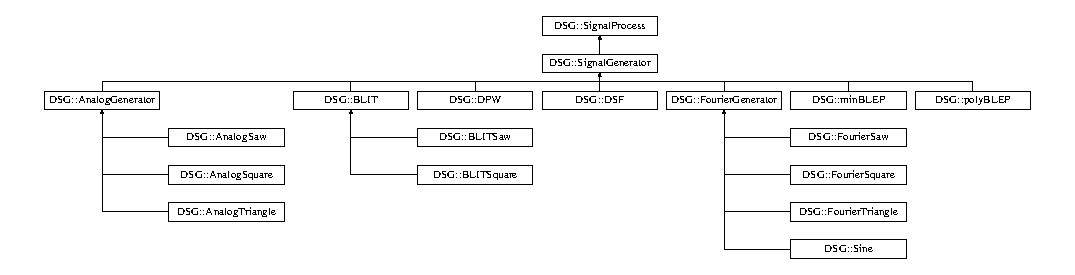
\includegraphics[height=3.245033cm]{classDSG_1_1SignalGenerator}
\end{center}
\end{figure}
\subsection*{Public Member Functions}
\begin{DoxyCompactItemize}
\item 
\hyperlink{classDSG_1_1SignalGenerator_a13ebda67fcdc880ef41aff501cc23fc3}{Signal\+Generator} ()
\item 
\hyperlink{classDSG_1_1SignalGenerator_a22c9bd8f74d6fabdf1104e5b9afbe08a}{Signal\+Generator} (double const \&frequency, double const \&phase\+\_\+offset)
\item 
virtual \hyperlink{classDSG_1_1SignalGenerator_a7b52d391974bc36a19fdcf617ad976cb}{$\sim$\+Signal\+Generator} ()
\item 
virtual bool \hyperlink{classDSG_1_1SignalGenerator_a95d485b68d874938ac93644b121607b9}{Perform} (\hyperlink{classDSG_1_1Sample}{Sample} \&signal)
\item 
virtual bool \hyperlink{classDSG_1_1SignalGenerator_abaa9aecd00b792d46166b91524b42db6}{Perform} (\hyperlink{classDSG_1_1RingBuffer}{Ring\+Buffer} \&signal)
\item 
virtual double const \& \hyperlink{classDSG_1_1SignalGenerator_aedac746c5a70818d120858542ecb7c45}{Frequency} () const 
\item 
virtual double const \& \hyperlink{classDSG_1_1SignalGenerator_ae3ce8d45bafabbd86a0f535b15c3cd46}{Frequency} (double const \&value)
\item 
virtual double const \& \hyperlink{classDSG_1_1SignalGenerator_a1ce521847edd0b837fd840998f906b4b}{Phase\+Offset} () const 
\item 
virtual double const \& \hyperlink{classDSG_1_1SignalGenerator_a08b71b1f30ba65e629642c570291dc0e}{Phase\+Offset} (double const \&value)
\item 
virtual bool \hyperlink{classDSG_1_1SignalProcess_afdb8220100418893950c1161dd24db67}{Perform} (\hyperlink{classDSG_1_1Sample_aaf2e30d73911eccea99b53eeee15b612}{Sample\+::\+Sample} \&signal)=0
\end{DoxyCompactItemize}
\subsection*{Protected Member Functions}
\begin{DoxyCompactItemize}
\item 
double \hyperlink{classDSG_1_1SignalGenerator_ac0d781b8673b3a283bf7c133290ede50}{\+\_\+pstep} ()
\item 
double \hyperlink{classDSG_1_1SignalGenerator_ae660eb4caa88b8d278f8d24d0908a487}{\+\_\+pstep\+\_\+rad} ()
\item 
void \hyperlink{classDSG_1_1SignalGenerator_a05baccb38d1e52860d4fcf7cb8430efc}{\+\_\+psync} ()
\end{DoxyCompactItemize}
\subsection*{Protected Attributes}
\begin{DoxyCompactItemize}
\item 
double \hyperlink{classDSG_1_1SignalGenerator_aa10f6c85d9adee901139ea7fb346f39d}{\+\_\+rate}
\item 
double \hyperlink{classDSG_1_1SignalGenerator_a67e296e3506dcdf09402c667cddff9ac}{\+\_\+frequency}
\item 
double \hyperlink{classDSG_1_1SignalGenerator_ac2271b582bf699275f077ecb642a8cd9}{\+\_\+phasor}
\end{DoxyCompactItemize}


\subsection{Detailed Description}
A Base Class extending the \hyperlink{classDSG_1_1SignalProcess}{Signal\+Process} A\+P\+I with functionality for signal generation. 

Definition at line 15 of file Signal\+Generator.\+h.



\subsection{Constructor \& Destructor Documentation}
\hypertarget{classDSG_1_1SignalGenerator_a13ebda67fcdc880ef41aff501cc23fc3}{\index{D\+S\+G\+::\+Signal\+Generator@{D\+S\+G\+::\+Signal\+Generator}!Signal\+Generator@{Signal\+Generator}}
\index{Signal\+Generator@{Signal\+Generator}!D\+S\+G\+::\+Signal\+Generator@{D\+S\+G\+::\+Signal\+Generator}}
\subsubsection[{Signal\+Generator}]{\setlength{\rightskip}{0pt plus 5cm}D\+S\+G\+::\+Signal\+Generator\+::\+Signal\+Generator (
\begin{DoxyParamCaption}
{}
\end{DoxyParamCaption}
)}}\label{classDSG_1_1SignalGenerator_a13ebda67fcdc880ef41aff501cc23fc3}


Definition at line 9 of file Signal\+Generator.\+cpp.


\begin{DoxyCode}
9                                    :\hyperlink{classDSG_1_1SignalGenerator_aa10f6c85d9adee901139ea7fb346f39d}{\_rate}(0),\_phase\_offset(0),\hyperlink{classDSG_1_1SignalGenerator_a67e296e3506dcdf09402c667cddff9ac}{\_frequency}(0),
      \hyperlink{classDSG_1_1SignalGenerator_ac2271b582bf699275f077ecb642a8cd9}{\_phasor}(0)\{
10 
11 \}
\end{DoxyCode}
\hypertarget{classDSG_1_1SignalGenerator_a22c9bd8f74d6fabdf1104e5b9afbe08a}{\index{D\+S\+G\+::\+Signal\+Generator@{D\+S\+G\+::\+Signal\+Generator}!Signal\+Generator@{Signal\+Generator}}
\index{Signal\+Generator@{Signal\+Generator}!D\+S\+G\+::\+Signal\+Generator@{D\+S\+G\+::\+Signal\+Generator}}
\subsubsection[{Signal\+Generator}]{\setlength{\rightskip}{0pt plus 5cm}D\+S\+G\+::\+Signal\+Generator\+::\+Signal\+Generator (
\begin{DoxyParamCaption}
\item[{double const \&}]{frequency, }
\item[{double const \&}]{phase\+\_\+offset}
\end{DoxyParamCaption}
)}}\label{classDSG_1_1SignalGenerator_a22c9bd8f74d6fabdf1104e5b9afbe08a}


Definition at line 12 of file Signal\+Generator.\+cpp.


\begin{DoxyCode}
12 :\hyperlink{classDSG_1_1SignalGenerator_aa10f6c85d9adee901139ea7fb346f39d}{\_rate}(frequency/ \hyperlink{namespaceDSG_a0c5c3a251b3688398da18138c5efe4bf}{Sample\_Rate}()),\hyperlink{classDSG_1_1SignalGenerator_a67e296e3506dcdf09402c667cddff9ac}{\_frequency}(frequency),\_phase\_offset(phase\_offset
      ),\hyperlink{classDSG_1_1SignalGenerator_ac2271b582bf699275f077ecb642a8cd9}{\_phasor}(0)\{\}
\end{DoxyCode}
\hypertarget{classDSG_1_1SignalGenerator_a7b52d391974bc36a19fdcf617ad976cb}{\index{D\+S\+G\+::\+Signal\+Generator@{D\+S\+G\+::\+Signal\+Generator}!````~Signal\+Generator@{$\sim$\+Signal\+Generator}}
\index{````~Signal\+Generator@{$\sim$\+Signal\+Generator}!D\+S\+G\+::\+Signal\+Generator@{D\+S\+G\+::\+Signal\+Generator}}
\subsubsection[{$\sim$\+Signal\+Generator}]{\setlength{\rightskip}{0pt plus 5cm}D\+S\+G\+::\+Signal\+Generator\+::$\sim$\+Signal\+Generator (
\begin{DoxyParamCaption}
{}
\end{DoxyParamCaption}
)\hspace{0.3cm}{\ttfamily [virtual]}}}\label{classDSG_1_1SignalGenerator_a7b52d391974bc36a19fdcf617ad976cb}


Definition at line 13 of file Signal\+Generator.\+cpp.


\begin{DoxyCode}
13 \{\}
\end{DoxyCode}


\subsection{Member Function Documentation}
\hypertarget{classDSG_1_1SignalGenerator_ac0d781b8673b3a283bf7c133290ede50}{\index{D\+S\+G\+::\+Signal\+Generator@{D\+S\+G\+::\+Signal\+Generator}!\+\_\+pstep@{\+\_\+pstep}}
\index{\+\_\+pstep@{\+\_\+pstep}!D\+S\+G\+::\+Signal\+Generator@{D\+S\+G\+::\+Signal\+Generator}}
\subsubsection[{\+\_\+pstep}]{\setlength{\rightskip}{0pt plus 5cm}double D\+S\+G\+::\+Signal\+Generator\+::\+\_\+pstep (
\begin{DoxyParamCaption}
{}
\end{DoxyParamCaption}
)\hspace{0.3cm}{\ttfamily [inline]}, {\ttfamily [protected]}}}\label{classDSG_1_1SignalGenerator_ac0d781b8673b3a283bf7c133290ede50}


Definition at line 52 of file Signal\+Generator.\+h.


\begin{DoxyCode}
52                                          \{
53         value = \hyperlink{classDSG_1_1SignalGenerator_ac2271b582bf699275f077ecb642a8cd9}{\_phasor};
54         \hyperlink{classDSG_1_1SignalGenerator_ac2271b582bf699275f077ecb642a8cd9}{\_phasor}+=\hyperlink{classDSG_1_1SignalGenerator_aa10f6c85d9adee901139ea7fb346f39d}{\_rate};
55         \hyperlink{classDSG_1_1SignalGenerator_ac2271b582bf699275f077ecb642a8cd9}{\_phasor}>1?\hyperlink{classDSG_1_1SignalGenerator_ac2271b582bf699275f077ecb642a8cd9}{\_phasor}-=1:0;\textcolor{comment}{//cheaper cheaper %1}
56         \textcolor{comment}{//\_phasor -= (unsigned long)\_phasor;//cheaper %1}
57         \textcolor{keywordflow}{return} value;
58     \}
\end{DoxyCode}
\hypertarget{classDSG_1_1SignalGenerator_ae660eb4caa88b8d278f8d24d0908a487}{\index{D\+S\+G\+::\+Signal\+Generator@{D\+S\+G\+::\+Signal\+Generator}!\+\_\+pstep\+\_\+rad@{\+\_\+pstep\+\_\+rad}}
\index{\+\_\+pstep\+\_\+rad@{\+\_\+pstep\+\_\+rad}!D\+S\+G\+::\+Signal\+Generator@{D\+S\+G\+::\+Signal\+Generator}}
\subsubsection[{\+\_\+pstep\+\_\+rad}]{\setlength{\rightskip}{0pt plus 5cm}double D\+S\+G\+::\+Signal\+Generator\+::\+\_\+pstep\+\_\+rad (
\begin{DoxyParamCaption}
{}
\end{DoxyParamCaption}
)\hspace{0.3cm}{\ttfamily [inline]}, {\ttfamily [protected]}}}\label{classDSG_1_1SignalGenerator_ae660eb4caa88b8d278f8d24d0908a487}


Definition at line 59 of file Signal\+Generator.\+h.


\begin{DoxyCode}
59                                              \{
60         \textcolor{keywordflow}{return} \hyperlink{PI_8h_a4912c64aec0c943b7985db6cb61ff83a}{TWOPI} * \hyperlink{classDSG_1_1SignalGenerator_ac0d781b8673b3a283bf7c133290ede50}{\_pstep}();
61     \}
\end{DoxyCode}
\hypertarget{classDSG_1_1SignalGenerator_a05baccb38d1e52860d4fcf7cb8430efc}{\index{D\+S\+G\+::\+Signal\+Generator@{D\+S\+G\+::\+Signal\+Generator}!\+\_\+psync@{\+\_\+psync}}
\index{\+\_\+psync@{\+\_\+psync}!D\+S\+G\+::\+Signal\+Generator@{D\+S\+G\+::\+Signal\+Generator}}
\subsubsection[{\+\_\+psync}]{\setlength{\rightskip}{0pt plus 5cm}void D\+S\+G\+::\+Signal\+Generator\+::\+\_\+psync (
\begin{DoxyParamCaption}
{}
\end{DoxyParamCaption}
)\hspace{0.3cm}{\ttfamily [inline]}, {\ttfamily [protected]}}}\label{classDSG_1_1SignalGenerator_a05baccb38d1e52860d4fcf7cb8430efc}


Definition at line 62 of file Signal\+Generator.\+h.


\begin{DoxyCode}
62                                        \{
63         \hyperlink{classDSG_1_1SignalGenerator_ac2271b582bf699275f077ecb642a8cd9}{\_phasor} = \_phase\_offset;
64     \}
\end{DoxyCode}
\hypertarget{classDSG_1_1SignalGenerator_aedac746c5a70818d120858542ecb7c45}{\index{D\+S\+G\+::\+Signal\+Generator@{D\+S\+G\+::\+Signal\+Generator}!Frequency@{Frequency}}
\index{Frequency@{Frequency}!D\+S\+G\+::\+Signal\+Generator@{D\+S\+G\+::\+Signal\+Generator}}
\subsubsection[{Frequency}]{\setlength{\rightskip}{0pt plus 5cm}double const \& D\+S\+G\+::\+Signal\+Generator\+::\+Frequency (
\begin{DoxyParamCaption}
{}
\end{DoxyParamCaption}
) const\hspace{0.3cm}{\ttfamily [virtual]}}}\label{classDSG_1_1SignalGenerator_aedac746c5a70818d120858542ecb7c45}


Definition at line 14 of file Signal\+Generator.\+cpp.


\begin{DoxyCode}
14                                                 \{
15     \textcolor{keywordflow}{return} \hyperlink{classDSG_1_1SignalGenerator_a67e296e3506dcdf09402c667cddff9ac}{\_frequency};
16 \}
\end{DoxyCode}
\hypertarget{classDSG_1_1SignalGenerator_ae3ce8d45bafabbd86a0f535b15c3cd46}{\index{D\+S\+G\+::\+Signal\+Generator@{D\+S\+G\+::\+Signal\+Generator}!Frequency@{Frequency}}
\index{Frequency@{Frequency}!D\+S\+G\+::\+Signal\+Generator@{D\+S\+G\+::\+Signal\+Generator}}
\subsubsection[{Frequency}]{\setlength{\rightskip}{0pt plus 5cm}double const \& D\+S\+G\+::\+Signal\+Generator\+::\+Frequency (
\begin{DoxyParamCaption}
\item[{double const \&}]{value}
\end{DoxyParamCaption}
)\hspace{0.3cm}{\ttfamily [virtual]}}}\label{classDSG_1_1SignalGenerator_ae3ce8d45bafabbd86a0f535b15c3cd46}


Reimplemented in \hyperlink{classDSG_1_1BLIT_a67b698a54f37c361945cae3e137af76f}{D\+S\+G\+::\+B\+L\+I\+T}, \hyperlink{classDSG_1_1FourierTriangle_aebb275eee9fb923636a8db5e4aa90b39}{D\+S\+G\+::\+Fourier\+Triangle}, \hyperlink{classDSG_1_1FourierSaw_a929602365c9b29f30f523fa07a29966e}{D\+S\+G\+::\+Fourier\+Saw}, and \hyperlink{classDSG_1_1FourierSquare_a80f94eabad633e105cfa673fdee332d6}{D\+S\+G\+::\+Fourier\+Square}.



Definition at line 17 of file Signal\+Generator.\+cpp.


\begin{DoxyCode}
17                                                               \{
18     \hyperlink{classDSG_1_1SignalGenerator_a67e296e3506dcdf09402c667cddff9ac}{\_frequency} = value;
19     \hyperlink{classDSG_1_1SignalGenerator_aa10f6c85d9adee901139ea7fb346f39d}{\_rate} = \hyperlink{classDSG_1_1SignalGenerator_a67e296e3506dcdf09402c667cddff9ac}{\_frequency}/ \hyperlink{namespaceDSG_a0c5c3a251b3688398da18138c5efe4bf}{Sample\_Rate}();
20     \textcolor{keywordflow}{return} \hyperlink{classDSG_1_1SignalGenerator_a67e296e3506dcdf09402c667cddff9ac}{\_frequency};
21 \}
\end{DoxyCode}
\hypertarget{classDSG_1_1SignalProcess_afdb8220100418893950c1161dd24db67}{\index{D\+S\+G\+::\+Signal\+Generator@{D\+S\+G\+::\+Signal\+Generator}!Perform@{Perform}}
\index{Perform@{Perform}!D\+S\+G\+::\+Signal\+Generator@{D\+S\+G\+::\+Signal\+Generator}}
\subsubsection[{Perform}]{\setlength{\rightskip}{0pt plus 5cm}virtual bool D\+S\+G\+::\+Signal\+Process\+::\+Perform (
\begin{DoxyParamCaption}
\item[{{\bf Sample\+::\+Sample} \&}]{signal}
\end{DoxyParamCaption}
)\hspace{0.3cm}{\ttfamily [inline]}, {\ttfamily [pure virtual]}, {\ttfamily [inherited]}}}\label{classDSG_1_1SignalProcess_afdb8220100418893950c1161dd24db67}
\hypertarget{classDSG_1_1SignalGenerator_a95d485b68d874938ac93644b121607b9}{\index{D\+S\+G\+::\+Signal\+Generator@{D\+S\+G\+::\+Signal\+Generator}!Perform@{Perform}}
\index{Perform@{Perform}!D\+S\+G\+::\+Signal\+Generator@{D\+S\+G\+::\+Signal\+Generator}}
\subsubsection[{Perform}]{\setlength{\rightskip}{0pt plus 5cm}bool D\+S\+G\+::\+Signal\+Generator\+::\+Perform (
\begin{DoxyParamCaption}
\item[{{\bf Sample} \&}]{signal}
\end{DoxyParamCaption}
)\hspace{0.3cm}{\ttfamily [inline]}, {\ttfamily [virtual]}}}\label{classDSG_1_1SignalGenerator_a95d485b68d874938ac93644b121607b9}


Reimplemented in \hyperlink{classDSG_1_1FourierGenerator_a7f5e34e65c1fe757318fb5b063dabde9}{D\+S\+G\+::\+Fourier\+Generator}, \hyperlink{classDSG_1_1BLIT_a0f769ac63ee884a6d3899b38d6c2944c}{D\+S\+G\+::\+B\+L\+I\+T}, \hyperlink{classDSG_1_1AnalogGenerator_ac50033964304239b514b7ee9d064bc75}{D\+S\+G\+::\+Analog\+Generator}, \hyperlink{classDSG_1_1FourierTriangle_ae927efb96f8d40f620dd02bdaaeef4d5}{D\+S\+G\+::\+Fourier\+Triangle}, \hyperlink{classDSG_1_1Sine_a04d925dc8c9a4b320f21697ce853a407}{D\+S\+G\+::\+Sine}, \hyperlink{classDSG_1_1FourierSaw_a3cc372cd7dd694f8b9cb70e504dd04a1}{D\+S\+G\+::\+Fourier\+Saw}, \hyperlink{classDSG_1_1AnalogSaw_ae52d07d0d03f6f1fb92c012cc52ae3eb}{D\+S\+G\+::\+Analog\+Saw}, \hyperlink{classDSG_1_1AnalogSquare_a93a4b464545a32f72491d3df490fd3f7}{D\+S\+G\+::\+Analog\+Square}, \hyperlink{classDSG_1_1AnalogTriangle_ac3edb87c395763d6894672b471850b05}{D\+S\+G\+::\+Analog\+Triangle}, and \hyperlink{classDSG_1_1FourierSquare_a3e9cfc95b3592eaf04fbcd61a3c68387}{D\+S\+G\+::\+Fourier\+Square}.



Definition at line 44 of file Signal\+Generator.\+h.


\begin{DoxyCode}
44                                                        \{
45         signal = 0;
46         \textcolor{keywordflow}{return} \textcolor{keyword}{false};
47     \}
\end{DoxyCode}
\hypertarget{classDSG_1_1SignalGenerator_abaa9aecd00b792d46166b91524b42db6}{\index{D\+S\+G\+::\+Signal\+Generator@{D\+S\+G\+::\+Signal\+Generator}!Perform@{Perform}}
\index{Perform@{Perform}!D\+S\+G\+::\+Signal\+Generator@{D\+S\+G\+::\+Signal\+Generator}}
\subsubsection[{Perform}]{\setlength{\rightskip}{0pt plus 5cm}bool D\+S\+G\+::\+Signal\+Generator\+::\+Perform (
\begin{DoxyParamCaption}
\item[{{\bf Ring\+Buffer} \&}]{signal}
\end{DoxyParamCaption}
)\hspace{0.3cm}{\ttfamily [inline]}, {\ttfamily [virtual]}}}\label{classDSG_1_1SignalGenerator_abaa9aecd00b792d46166b91524b42db6}


Implements \hyperlink{classDSG_1_1SignalProcess_a9df44fe60cca01c3c697283408cecf4d}{D\+S\+G\+::\+Signal\+Process}.



Reimplemented in \hyperlink{classDSG_1_1FourierGenerator_a8b2aca91155dbb524aaf13867f273188}{D\+S\+G\+::\+Fourier\+Generator}, \hyperlink{classDSG_1_1BLIT_ae464457074d366c46f42b53b59d82ecb}{D\+S\+G\+::\+B\+L\+I\+T}, \hyperlink{classDSG_1_1AnalogGenerator_a1b4f1d4af926fcc3e9571db7960c8706}{D\+S\+G\+::\+Analog\+Generator}, \hyperlink{classDSG_1_1FourierTriangle_a017e2b59123ff3afa9a5c0e833e5f482}{D\+S\+G\+::\+Fourier\+Triangle}, \hyperlink{classDSG_1_1Sine_a6408fedf61f1f2a4026261d181997afc}{D\+S\+G\+::\+Sine}, \hyperlink{classDSG_1_1FourierSaw_a76b78874feebbc89d00656fec4bfd57a}{D\+S\+G\+::\+Fourier\+Saw}, \hyperlink{classDSG_1_1AnalogSaw_a14dbd5c7faf6559b9ea79f8eb1ad6af5}{D\+S\+G\+::\+Analog\+Saw}, \hyperlink{classDSG_1_1AnalogSquare_a1d9c8a380775a7e4f6e0aa8fb1b05af6}{D\+S\+G\+::\+Analog\+Square}, \hyperlink{classDSG_1_1AnalogTriangle_a9456183af28d98ccf3daa85b8ad12b52}{D\+S\+G\+::\+Analog\+Triangle}, and \hyperlink{classDSG_1_1FourierSquare_ad9999119d9efc453329ed4b3eaf5f226}{D\+S\+G\+::\+Fourier\+Square}.



Definition at line 48 of file Signal\+Generator.\+h.


\begin{DoxyCode}
48                                                            \{
49         signal.Flush();
50         \textcolor{keywordflow}{return} \textcolor{keyword}{false};
51     \}
\end{DoxyCode}
\hypertarget{classDSG_1_1SignalGenerator_a1ce521847edd0b837fd840998f906b4b}{\index{D\+S\+G\+::\+Signal\+Generator@{D\+S\+G\+::\+Signal\+Generator}!Phase\+Offset@{Phase\+Offset}}
\index{Phase\+Offset@{Phase\+Offset}!D\+S\+G\+::\+Signal\+Generator@{D\+S\+G\+::\+Signal\+Generator}}
\subsubsection[{Phase\+Offset}]{\setlength{\rightskip}{0pt plus 5cm}double const \& D\+S\+G\+::\+Signal\+Generator\+::\+Phase\+Offset (
\begin{DoxyParamCaption}
{}
\end{DoxyParamCaption}
) const\hspace{0.3cm}{\ttfamily [virtual]}}}\label{classDSG_1_1SignalGenerator_a1ce521847edd0b837fd840998f906b4b}


Definition at line 22 of file Signal\+Generator.\+cpp.


\begin{DoxyCode}
22                                                   \{
23     \textcolor{keywordflow}{return} \_phase\_offset;
24 \}
\end{DoxyCode}
\hypertarget{classDSG_1_1SignalGenerator_a08b71b1f30ba65e629642c570291dc0e}{\index{D\+S\+G\+::\+Signal\+Generator@{D\+S\+G\+::\+Signal\+Generator}!Phase\+Offset@{Phase\+Offset}}
\index{Phase\+Offset@{Phase\+Offset}!D\+S\+G\+::\+Signal\+Generator@{D\+S\+G\+::\+Signal\+Generator}}
\subsubsection[{Phase\+Offset}]{\setlength{\rightskip}{0pt plus 5cm}double const \& D\+S\+G\+::\+Signal\+Generator\+::\+Phase\+Offset (
\begin{DoxyParamCaption}
\item[{double const \&}]{value}
\end{DoxyParamCaption}
)\hspace{0.3cm}{\ttfamily [virtual]}}}\label{classDSG_1_1SignalGenerator_a08b71b1f30ba65e629642c570291dc0e}


Definition at line 25 of file Signal\+Generator.\+cpp.


\begin{DoxyCode}
25                                                                 \{
26     \_phase\_offset-=value;
27     \hyperlink{classDSG_1_1SignalGenerator_ac2271b582bf699275f077ecb642a8cd9}{\_phasor}-=\_phase\_offset;
28     \_phase\_offset=value;
29     \textcolor{keywordflow}{return} \_phase\_offset;
30 \}\end{DoxyCode}


\subsection{Member Data Documentation}
\hypertarget{classDSG_1_1SignalGenerator_a67e296e3506dcdf09402c667cddff9ac}{\index{D\+S\+G\+::\+Signal\+Generator@{D\+S\+G\+::\+Signal\+Generator}!\+\_\+frequency@{\+\_\+frequency}}
\index{\+\_\+frequency@{\+\_\+frequency}!D\+S\+G\+::\+Signal\+Generator@{D\+S\+G\+::\+Signal\+Generator}}
\subsubsection[{\+\_\+frequency}]{\setlength{\rightskip}{0pt plus 5cm}double D\+S\+G\+::\+Signal\+Generator\+::\+\_\+frequency\hspace{0.3cm}{\ttfamily [protected]}}}\label{classDSG_1_1SignalGenerator_a67e296e3506dcdf09402c667cddff9ac}


Definition at line 28 of file Signal\+Generator.\+h.

\hypertarget{classDSG_1_1SignalGenerator_ac2271b582bf699275f077ecb642a8cd9}{\index{D\+S\+G\+::\+Signal\+Generator@{D\+S\+G\+::\+Signal\+Generator}!\+\_\+phasor@{\+\_\+phasor}}
\index{\+\_\+phasor@{\+\_\+phasor}!D\+S\+G\+::\+Signal\+Generator@{D\+S\+G\+::\+Signal\+Generator}}
\subsubsection[{\+\_\+phasor}]{\setlength{\rightskip}{0pt plus 5cm}double D\+S\+G\+::\+Signal\+Generator\+::\+\_\+phasor\hspace{0.3cm}{\ttfamily [protected]}}}\label{classDSG_1_1SignalGenerator_ac2271b582bf699275f077ecb642a8cd9}


Definition at line 38 of file Signal\+Generator.\+h.

\hypertarget{classDSG_1_1SignalGenerator_aa10f6c85d9adee901139ea7fb346f39d}{\index{D\+S\+G\+::\+Signal\+Generator@{D\+S\+G\+::\+Signal\+Generator}!\+\_\+rate@{\+\_\+rate}}
\index{\+\_\+rate@{\+\_\+rate}!D\+S\+G\+::\+Signal\+Generator@{D\+S\+G\+::\+Signal\+Generator}}
\subsubsection[{\+\_\+rate}]{\setlength{\rightskip}{0pt plus 5cm}double D\+S\+G\+::\+Signal\+Generator\+::\+\_\+rate\hspace{0.3cm}{\ttfamily [protected]}}}\label{classDSG_1_1SignalGenerator_aa10f6c85d9adee901139ea7fb346f39d}


Definition at line 27 of file Signal\+Generator.\+h.



The documentation for this class was generated from the following files\+:\begin{DoxyCompactItemize}
\item 
/\+Users/alexanderzywicki/\+Documents/\+School\+\_\+\+Stuff/\+Fall\+\_\+2014/\+Digital\+\_\+\+Signal\+\_\+\+Generation\+\_\+and\+\_\+\+Analysis/src/include/\hyperlink{SignalGenerator_8h}{Signal\+Generator.\+h}\item 
/\+Users/alexanderzywicki/\+Documents/\+School\+\_\+\+Stuff/\+Fall\+\_\+2014/\+Digital\+\_\+\+Signal\+\_\+\+Generation\+\_\+and\+\_\+\+Analysis/src/\hyperlink{SignalGenerator_8cpp}{Signal\+Generator.\+cpp}\end{DoxyCompactItemize}

\hypertarget{classDSG_1_1SignalProcess}{\section{D\+S\+G\+:\+:Signal\+Process Class Reference}
\label{classDSG_1_1SignalProcess}\index{D\+S\+G\+::\+Signal\+Process@{D\+S\+G\+::\+Signal\+Process}}
}


An Abstract Base Class defining the basics A\+P\+I needed for audio generation.  




{\ttfamily \#include $<$Signal\+Process.\+h$>$}

Inheritance diagram for D\+S\+G\+:\+:Signal\+Process\+:\begin{figure}[H]
\begin{center}
\leavevmode
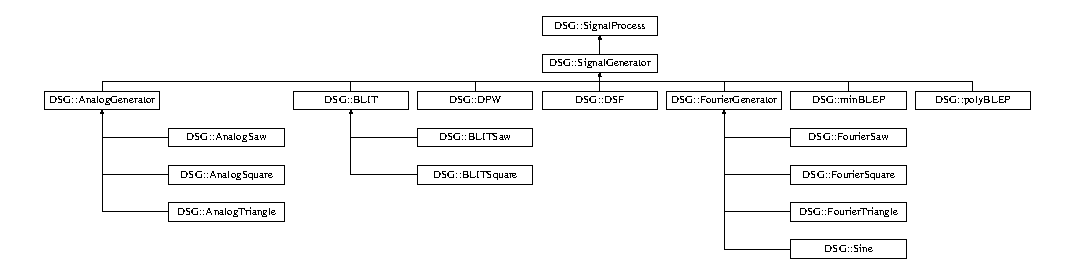
\includegraphics[height=3.245033cm]{classDSG_1_1SignalProcess}
\end{center}
\end{figure}
\subsection*{Public Member Functions}
\begin{DoxyCompactItemize}
\item 
\hyperlink{classDSG_1_1SignalProcess_a3fd4347483bcf3cc0a3d7bf98ff56218}{Signal\+Process} ()
\item 
virtual \hyperlink{classDSG_1_1SignalProcess_ad9b6a758241a092ddc38e13effc9553f}{$\sim$\+Signal\+Process} ()
\item 
virtual bool \hyperlink{classDSG_1_1SignalProcess_afdb8220100418893950c1161dd24db67}{Perform} (\hyperlink{classDSG_1_1Sample_aaf2e30d73911eccea99b53eeee15b612}{Sample\+::\+Sample} \&signal)=0
\item 
virtual bool \hyperlink{classDSG_1_1SignalProcess_a9df44fe60cca01c3c697283408cecf4d}{Perform} (\hyperlink{classDSG_1_1RingBuffer}{Ring\+Buffer} \&signal)=0
\end{DoxyCompactItemize}


\subsection{Detailed Description}
An Abstract Base Class defining the basics A\+P\+I needed for audio generation. 

Definition at line 16 of file Signal\+Process.\+h.



\subsection{Constructor \& Destructor Documentation}
\hypertarget{classDSG_1_1SignalProcess_a3fd4347483bcf3cc0a3d7bf98ff56218}{\index{D\+S\+G\+::\+Signal\+Process@{D\+S\+G\+::\+Signal\+Process}!Signal\+Process@{Signal\+Process}}
\index{Signal\+Process@{Signal\+Process}!D\+S\+G\+::\+Signal\+Process@{D\+S\+G\+::\+Signal\+Process}}
\subsubsection[{Signal\+Process}]{\setlength{\rightskip}{0pt plus 5cm}D\+S\+G\+::\+Signal\+Process\+::\+Signal\+Process (
\begin{DoxyParamCaption}
{}
\end{DoxyParamCaption}
)}}\label{classDSG_1_1SignalProcess_a3fd4347483bcf3cc0a3d7bf98ff56218}


Definition at line 9 of file Signal\+Process.\+cpp.


\begin{DoxyCode}
9 \{\}
\end{DoxyCode}
\hypertarget{classDSG_1_1SignalProcess_ad9b6a758241a092ddc38e13effc9553f}{\index{D\+S\+G\+::\+Signal\+Process@{D\+S\+G\+::\+Signal\+Process}!````~Signal\+Process@{$\sim$\+Signal\+Process}}
\index{````~Signal\+Process@{$\sim$\+Signal\+Process}!D\+S\+G\+::\+Signal\+Process@{D\+S\+G\+::\+Signal\+Process}}
\subsubsection[{$\sim$\+Signal\+Process}]{\setlength{\rightskip}{0pt plus 5cm}D\+S\+G\+::\+Signal\+Process\+::$\sim$\+Signal\+Process (
\begin{DoxyParamCaption}
{}
\end{DoxyParamCaption}
)\hspace{0.3cm}{\ttfamily [virtual]}}}\label{classDSG_1_1SignalProcess_ad9b6a758241a092ddc38e13effc9553f}


Definition at line 10 of file Signal\+Process.\+cpp.


\begin{DoxyCode}
10 \{\}\end{DoxyCode}


\subsection{Member Function Documentation}
\hypertarget{classDSG_1_1SignalProcess_afdb8220100418893950c1161dd24db67}{\index{D\+S\+G\+::\+Signal\+Process@{D\+S\+G\+::\+Signal\+Process}!Perform@{Perform}}
\index{Perform@{Perform}!D\+S\+G\+::\+Signal\+Process@{D\+S\+G\+::\+Signal\+Process}}
\subsubsection[{Perform}]{\setlength{\rightskip}{0pt plus 5cm}virtual bool D\+S\+G\+::\+Signal\+Process\+::\+Perform (
\begin{DoxyParamCaption}
\item[{{\bf Sample\+::\+Sample} \&}]{signal}
\end{DoxyParamCaption}
)\hspace{0.3cm}{\ttfamily [inline]}, {\ttfamily [pure virtual]}}}\label{classDSG_1_1SignalProcess_afdb8220100418893950c1161dd24db67}
\hypertarget{classDSG_1_1SignalProcess_a9df44fe60cca01c3c697283408cecf4d}{\index{D\+S\+G\+::\+Signal\+Process@{D\+S\+G\+::\+Signal\+Process}!Perform@{Perform}}
\index{Perform@{Perform}!D\+S\+G\+::\+Signal\+Process@{D\+S\+G\+::\+Signal\+Process}}
\subsubsection[{Perform}]{\setlength{\rightskip}{0pt plus 5cm}virtual bool D\+S\+G\+::\+Signal\+Process\+::\+Perform (
\begin{DoxyParamCaption}
\item[{{\bf Ring\+Buffer} \&}]{signal}
\end{DoxyParamCaption}
)\hspace{0.3cm}{\ttfamily [inline]}, {\ttfamily [pure virtual]}}}\label{classDSG_1_1SignalProcess_a9df44fe60cca01c3c697283408cecf4d}


Implemented in \hyperlink{classDSG_1_1FourierGenerator_a8b2aca91155dbb524aaf13867f273188}{D\+S\+G\+::\+Fourier\+Generator}, \hyperlink{classDSG_1_1BLIT_ae464457074d366c46f42b53b59d82ecb}{D\+S\+G\+::\+B\+L\+I\+T}, \hyperlink{classDSG_1_1AnalogGenerator_a1b4f1d4af926fcc3e9571db7960c8706}{D\+S\+G\+::\+Analog\+Generator}, \hyperlink{classDSG_1_1FourierTriangle_a017e2b59123ff3afa9a5c0e833e5f482}{D\+S\+G\+::\+Fourier\+Triangle}, \hyperlink{classDSG_1_1Sine_a6408fedf61f1f2a4026261d181997afc}{D\+S\+G\+::\+Sine}, \hyperlink{classDSG_1_1FourierSaw_a76b78874feebbc89d00656fec4bfd57a}{D\+S\+G\+::\+Fourier\+Saw}, \hyperlink{classDSG_1_1AnalogSaw_a14dbd5c7faf6559b9ea79f8eb1ad6af5}{D\+S\+G\+::\+Analog\+Saw}, \hyperlink{classDSG_1_1AnalogSquare_a1d9c8a380775a7e4f6e0aa8fb1b05af6}{D\+S\+G\+::\+Analog\+Square}, \hyperlink{classDSG_1_1AnalogTriangle_a9456183af28d98ccf3daa85b8ad12b52}{D\+S\+G\+::\+Analog\+Triangle}, \hyperlink{classDSG_1_1FourierSquare_ad9999119d9efc453329ed4b3eaf5f226}{D\+S\+G\+::\+Fourier\+Square}, and \hyperlink{classDSG_1_1SignalGenerator_abaa9aecd00b792d46166b91524b42db6}{D\+S\+G\+::\+Signal\+Generator}.



The documentation for this class was generated from the following files\+:\begin{DoxyCompactItemize}
\item 
/\+Users/alexanderzywicki/\+Documents/\+School\+\_\+\+Stuff/\+Fall\+\_\+2014/\+Digital\+\_\+\+Signal\+\_\+\+Generation\+\_\+and\+\_\+\+Analysis/src/include/\hyperlink{SignalProcess_8h}{Signal\+Process.\+h}\item 
/\+Users/alexanderzywicki/\+Documents/\+School\+\_\+\+Stuff/\+Fall\+\_\+2014/\+Digital\+\_\+\+Signal\+\_\+\+Generation\+\_\+and\+\_\+\+Analysis/src/\hyperlink{SignalProcess_8cpp}{Signal\+Process.\+cpp}\end{DoxyCompactItemize}

\hypertarget{classDSG_1_1Sine}{\section{D\+S\+G\+:\+:Sine Class Reference}
\label{classDSG_1_1Sine}\index{D\+S\+G\+::\+Sine@{D\+S\+G\+::\+Sine}}
}


\hyperlink{classDSG_1_1Sine}{Sine} Wave Generator.  




{\ttfamily \#include $<$Sine.\+h$>$}

Inheritance diagram for D\+S\+G\+:\+:Sine\+:\begin{figure}[H]
\begin{center}
\leavevmode
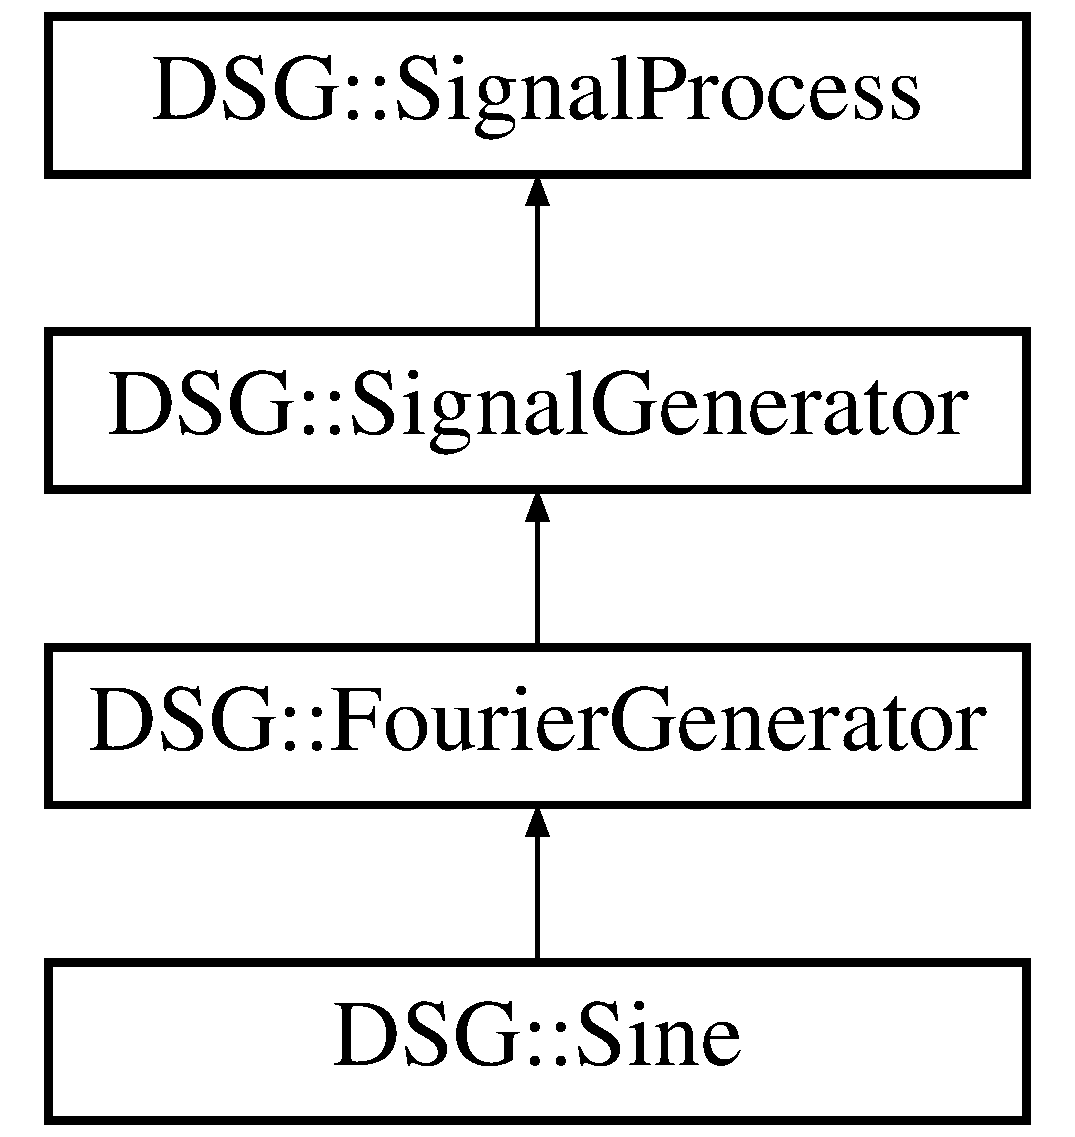
\includegraphics[height=4.000000cm]{classDSG_1_1Sine}
\end{center}
\end{figure}
\subsection*{Public Member Functions}
\begin{DoxyCompactItemize}
\item 
\hyperlink{classDSG_1_1Sine_ab8dcc9f9885ab30c3aa81719c764d392}{Sine} ()
\item 
\hyperlink{classDSG_1_1Sine_aadedca66967e66cc615d8c5ce3eec6e8}{Sine} (double const \&frequency, double const \&phase\+\_\+offset)
\item 
virtual \hyperlink{classDSG_1_1Sine_acf3012137866fa71d727d2ccfb59ddac}{$\sim$\+Sine} ()
\item 
virtual bool \hyperlink{classDSG_1_1Sine_a04d925dc8c9a4b320f21697ce853a407}{Perform} (\hyperlink{classDSG_1_1Sample}{Sample} \&signal)
\item 
virtual bool \hyperlink{classDSG_1_1Sine_a6408fedf61f1f2a4026261d181997afc}{Perform} (\hyperlink{classDSG_1_1RingBuffer}{Ring\+Buffer} \&signal)
\item 
virtual bool \hyperlink{classDSG_1_1SignalProcess_afdb8220100418893950c1161dd24db67}{Perform} (\hyperlink{classDSG_1_1Sample_aaf2e30d73911eccea99b53eeee15b612}{Sample\+::\+Sample} \&signal)=0
\item 
virtual double const \& \hyperlink{classDSG_1_1SignalGenerator_aedac746c5a70818d120858542ecb7c45}{Frequency} () const 
\item 
virtual double const \& \hyperlink{classDSG_1_1SignalGenerator_ae3ce8d45bafabbd86a0f535b15c3cd46}{Frequency} (double const \&value)
\item 
virtual double const \& \hyperlink{classDSG_1_1SignalGenerator_a1ce521847edd0b837fd840998f906b4b}{Phase\+Offset} () const 
\item 
virtual double const \& \hyperlink{classDSG_1_1SignalGenerator_a08b71b1f30ba65e629642c570291dc0e}{Phase\+Offset} (double const \&value)
\end{DoxyCompactItemize}
\subsection*{Protected Member Functions}
\begin{DoxyCompactItemize}
\item 
unsigned long \hyperlink{classDSG_1_1FourierGenerator_a6b6e3bbad8ff7443d9ed71f4cdf76739}{\+\_\+max\+Harms} (double \+\_\+frq)
\item 
double \hyperlink{classDSG_1_1SignalGenerator_ac0d781b8673b3a283bf7c133290ede50}{\+\_\+pstep} ()
\item 
double \hyperlink{classDSG_1_1SignalGenerator_ae660eb4caa88b8d278f8d24d0908a487}{\+\_\+pstep\+\_\+rad} ()
\item 
void \hyperlink{classDSG_1_1SignalGenerator_a05baccb38d1e52860d4fcf7cb8430efc}{\+\_\+psync} ()
\end{DoxyCompactItemize}
\subsection*{Protected Attributes}
\begin{DoxyCompactItemize}
\item 
\hyperlink{classDSG_1_1Sample}{Sample} \hyperlink{classDSG_1_1FourierGenerator_ab96bed1cd59c42e82a689036e5c62bef}{\+\_\+sample}
\item 
\hyperlink{classDSG_1_1Sample}{Sample} \hyperlink{classDSG_1_1FourierGenerator_a6b7f2439b26914cc9df6b6975a2cedac}{\+\_\+storage}
\item 
double \hyperlink{classDSG_1_1SignalGenerator_aa10f6c85d9adee901139ea7fb346f39d}{\+\_\+rate}
\item 
double \hyperlink{classDSG_1_1SignalGenerator_a67e296e3506dcdf09402c667cddff9ac}{\+\_\+frequency}
\item 
double \hyperlink{classDSG_1_1SignalGenerator_ac2271b582bf699275f077ecb642a8cd9}{\+\_\+phasor}
\end{DoxyCompactItemize}
\subsection*{Static Protected Attributes}
\begin{DoxyCompactItemize}
\item 
static \hyperlink{classDSG_1_1Backend_1_1HarmonicTable}{D\+S\+G\+::\+Backend\+::\+Harmonic\+Table} \hyperlink{classDSG_1_1FourierGenerator_aedac2cf90997418836d064c90540249d}{\+\_\+harmonic\+Table}
\end{DoxyCompactItemize}


\subsection{Detailed Description}
\hyperlink{classDSG_1_1Sine}{Sine} Wave Generator. 

Definition at line 19 of file Sine.\+h.



\subsection{Constructor \& Destructor Documentation}
\hypertarget{classDSG_1_1Sine_ab8dcc9f9885ab30c3aa81719c764d392}{\index{D\+S\+G\+::\+Sine@{D\+S\+G\+::\+Sine}!Sine@{Sine}}
\index{Sine@{Sine}!D\+S\+G\+::\+Sine@{D\+S\+G\+::\+Sine}}
\subsubsection[{Sine}]{\setlength{\rightskip}{0pt plus 5cm}D\+S\+G\+::\+Sine\+::\+Sine (
\begin{DoxyParamCaption}
{}
\end{DoxyParamCaption}
)}}\label{classDSG_1_1Sine_ab8dcc9f9885ab30c3aa81719c764d392}


Definition at line 12 of file Sine.\+cpp.


\begin{DoxyCode}
12 :\hyperlink{classDSG_1_1FourierGenerator_a43fa07fd160c41fd679a5bd2843a5b0e}{FourierGenerator}()\{\}
\end{DoxyCode}
\hypertarget{classDSG_1_1Sine_aadedca66967e66cc615d8c5ce3eec6e8}{\index{D\+S\+G\+::\+Sine@{D\+S\+G\+::\+Sine}!Sine@{Sine}}
\index{Sine@{Sine}!D\+S\+G\+::\+Sine@{D\+S\+G\+::\+Sine}}
\subsubsection[{Sine}]{\setlength{\rightskip}{0pt plus 5cm}D\+S\+G\+::\+Sine\+::\+Sine (
\begin{DoxyParamCaption}
\item[{double const \&}]{frequency, }
\item[{double const \&}]{phase\+\_\+offset}
\end{DoxyParamCaption}
)}}\label{classDSG_1_1Sine_aadedca66967e66cc615d8c5ce3eec6e8}


Definition at line 13 of file Sine.\+cpp.


\begin{DoxyCode}
13                                                                :\hyperlink{classDSG_1_1FourierGenerator_a43fa07fd160c41fd679a5bd2843a5b0e}{FourierGenerator}(frequency,
      phase\_offset)\{
14     \hyperlink{classDSG_1_1FourierGenerator_ab96bed1cd59c42e82a689036e5c62bef}{\_sample}=0;
15     \hyperlink{classDSG_1_1FourierGenerator_a6b7f2439b26914cc9df6b6975a2cedac}{\_storage}=0;
16 \}
\end{DoxyCode}
\hypertarget{classDSG_1_1Sine_acf3012137866fa71d727d2ccfb59ddac}{\index{D\+S\+G\+::\+Sine@{D\+S\+G\+::\+Sine}!````~Sine@{$\sim$\+Sine}}
\index{````~Sine@{$\sim$\+Sine}!D\+S\+G\+::\+Sine@{D\+S\+G\+::\+Sine}}
\subsubsection[{$\sim$\+Sine}]{\setlength{\rightskip}{0pt plus 5cm}D\+S\+G\+::\+Sine\+::$\sim$\+Sine (
\begin{DoxyParamCaption}
{}
\end{DoxyParamCaption}
)\hspace{0.3cm}{\ttfamily [virtual]}}}\label{classDSG_1_1Sine_acf3012137866fa71d727d2ccfb59ddac}


Definition at line 17 of file Sine.\+cpp.


\begin{DoxyCode}
17 \{\}
\end{DoxyCode}


\subsection{Member Function Documentation}
\hypertarget{classDSG_1_1FourierGenerator_a6b6e3bbad8ff7443d9ed71f4cdf76739}{\index{D\+S\+G\+::\+Sine@{D\+S\+G\+::\+Sine}!\+\_\+max\+Harms@{\+\_\+max\+Harms}}
\index{\+\_\+max\+Harms@{\+\_\+max\+Harms}!D\+S\+G\+::\+Sine@{D\+S\+G\+::\+Sine}}
\subsubsection[{\+\_\+max\+Harms}]{\setlength{\rightskip}{0pt plus 5cm}unsigned long D\+S\+G\+::\+Fourier\+Generator\+::\+\_\+max\+Harms (
\begin{DoxyParamCaption}
\item[{double}]{\+\_\+frq}
\end{DoxyParamCaption}
)\hspace{0.3cm}{\ttfamily [inline]}, {\ttfamily [protected]}, {\ttfamily [inherited]}}}\label{classDSG_1_1FourierGenerator_a6b6e3bbad8ff7443d9ed71f4cdf76739}


Definition at line 53 of file Fourier\+Generator.\+h.


\begin{DoxyCode}
53                                                                    \{
54             \textcolor{comment}{//double softLim = 0.45;}
55             \textcolor{comment}{//double hardLim = 0.5;}
56             
57             \textcolor{keywordtype}{double} \_s =  \hyperlink{namespaceDSG_a0c5c3a251b3688398da18138c5efe4bf}{Sample\_Rate}()* (20000.0/ \hyperlink{namespaceDSG_a0c5c3a251b3688398da18138c5efe4bf}{Sample\_Rate}());\textcolor{comment}{//uses harmonic roll
       of based on max human hearing and sample rate}
58             \_s/=\_frq;
59             \textcolor{keywordflow}{return} trunc(\_s);
60         \}
\end{DoxyCode}
\hypertarget{classDSG_1_1SignalGenerator_ac0d781b8673b3a283bf7c133290ede50}{\index{D\+S\+G\+::\+Sine@{D\+S\+G\+::\+Sine}!\+\_\+pstep@{\+\_\+pstep}}
\index{\+\_\+pstep@{\+\_\+pstep}!D\+S\+G\+::\+Sine@{D\+S\+G\+::\+Sine}}
\subsubsection[{\+\_\+pstep}]{\setlength{\rightskip}{0pt plus 5cm}double D\+S\+G\+::\+Signal\+Generator\+::\+\_\+pstep (
\begin{DoxyParamCaption}
{}
\end{DoxyParamCaption}
)\hspace{0.3cm}{\ttfamily [inline]}, {\ttfamily [protected]}, {\ttfamily [inherited]}}}\label{classDSG_1_1SignalGenerator_ac0d781b8673b3a283bf7c133290ede50}


Definition at line 64 of file Signal\+Generator.\+h.


\begin{DoxyCode}
64                                          \{
65         value = \hyperlink{classDSG_1_1SignalGenerator_ac2271b582bf699275f077ecb642a8cd9}{\_phasor};
66         \hyperlink{classDSG_1_1SignalGenerator_ac2271b582bf699275f077ecb642a8cd9}{\_phasor}+=\hyperlink{classDSG_1_1SignalGenerator_aa10f6c85d9adee901139ea7fb346f39d}{\_rate};
67         \hyperlink{classDSG_1_1SignalGenerator_ac2271b582bf699275f077ecb642a8cd9}{\_phasor}>1?\hyperlink{classDSG_1_1SignalGenerator_ac2271b582bf699275f077ecb642a8cd9}{\_phasor}-=1:0;\textcolor{comment}{//cheaper cheaper %1}
68         \textcolor{comment}{//\_phasor -= (unsigned long)\_phasor;//cheaper %1}
69         \textcolor{keywordflow}{return} value;
70     \}
\end{DoxyCode}
\hypertarget{classDSG_1_1SignalGenerator_ae660eb4caa88b8d278f8d24d0908a487}{\index{D\+S\+G\+::\+Sine@{D\+S\+G\+::\+Sine}!\+\_\+pstep\+\_\+rad@{\+\_\+pstep\+\_\+rad}}
\index{\+\_\+pstep\+\_\+rad@{\+\_\+pstep\+\_\+rad}!D\+S\+G\+::\+Sine@{D\+S\+G\+::\+Sine}}
\subsubsection[{\+\_\+pstep\+\_\+rad}]{\setlength{\rightskip}{0pt plus 5cm}double D\+S\+G\+::\+Signal\+Generator\+::\+\_\+pstep\+\_\+rad (
\begin{DoxyParamCaption}
{}
\end{DoxyParamCaption}
)\hspace{0.3cm}{\ttfamily [inline]}, {\ttfamily [protected]}, {\ttfamily [inherited]}}}\label{classDSG_1_1SignalGenerator_ae660eb4caa88b8d278f8d24d0908a487}


Definition at line 71 of file Signal\+Generator.\+h.


\begin{DoxyCode}
71                                              \{
72         \textcolor{keywordflow}{return} \hyperlink{PI_8h_a4912c64aec0c943b7985db6cb61ff83a}{TWOPI} * \hyperlink{classDSG_1_1SignalGenerator_ac0d781b8673b3a283bf7c133290ede50}{\_pstep}();
73     \}
\end{DoxyCode}
\hypertarget{classDSG_1_1SignalGenerator_a05baccb38d1e52860d4fcf7cb8430efc}{\index{D\+S\+G\+::\+Sine@{D\+S\+G\+::\+Sine}!\+\_\+psync@{\+\_\+psync}}
\index{\+\_\+psync@{\+\_\+psync}!D\+S\+G\+::\+Sine@{D\+S\+G\+::\+Sine}}
\subsubsection[{\+\_\+psync}]{\setlength{\rightskip}{0pt plus 5cm}void D\+S\+G\+::\+Signal\+Generator\+::\+\_\+psync (
\begin{DoxyParamCaption}
{}
\end{DoxyParamCaption}
)\hspace{0.3cm}{\ttfamily [inline]}, {\ttfamily [protected]}, {\ttfamily [inherited]}}}\label{classDSG_1_1SignalGenerator_a05baccb38d1e52860d4fcf7cb8430efc}


Definition at line 74 of file Signal\+Generator.\+h.


\begin{DoxyCode}
74                                        \{
75         \hyperlink{classDSG_1_1SignalGenerator_ac2271b582bf699275f077ecb642a8cd9}{\_phasor} = \_phase\_offset;
76     \}
\end{DoxyCode}
\hypertarget{classDSG_1_1SignalGenerator_aedac746c5a70818d120858542ecb7c45}{\index{D\+S\+G\+::\+Sine@{D\+S\+G\+::\+Sine}!Frequency@{Frequency}}
\index{Frequency@{Frequency}!D\+S\+G\+::\+Sine@{D\+S\+G\+::\+Sine}}
\subsubsection[{Frequency}]{\setlength{\rightskip}{0pt plus 5cm}double const \& D\+S\+G\+::\+Signal\+Generator\+::\+Frequency (
\begin{DoxyParamCaption}
{}
\end{DoxyParamCaption}
) const\hspace{0.3cm}{\ttfamily [virtual]}, {\ttfamily [inherited]}}}\label{classDSG_1_1SignalGenerator_aedac746c5a70818d120858542ecb7c45}


Definition at line 16 of file Signal\+Generator.\+cpp.


\begin{DoxyCode}
16                                                 \{
17     \textcolor{keywordflow}{return} \hyperlink{classDSG_1_1SignalGenerator_a67e296e3506dcdf09402c667cddff9ac}{\_frequency};
18 \}
\end{DoxyCode}
\hypertarget{classDSG_1_1SignalGenerator_ae3ce8d45bafabbd86a0f535b15c3cd46}{\index{D\+S\+G\+::\+Sine@{D\+S\+G\+::\+Sine}!Frequency@{Frequency}}
\index{Frequency@{Frequency}!D\+S\+G\+::\+Sine@{D\+S\+G\+::\+Sine}}
\subsubsection[{Frequency}]{\setlength{\rightskip}{0pt plus 5cm}double const \& D\+S\+G\+::\+Signal\+Generator\+::\+Frequency (
\begin{DoxyParamCaption}
\item[{double const \&}]{value}
\end{DoxyParamCaption}
)\hspace{0.3cm}{\ttfamily [virtual]}, {\ttfamily [inherited]}}}\label{classDSG_1_1SignalGenerator_ae3ce8d45bafabbd86a0f535b15c3cd46}


Reimplemented in \hyperlink{classDSG_1_1BLIT_a67b698a54f37c361945cae3e137af76f}{D\+S\+G\+::\+B\+L\+I\+T}, \hyperlink{classDSG_1_1FourierSaw_a929602365c9b29f30f523fa07a29966e}{D\+S\+G\+::\+Fourier\+Saw}, \hyperlink{classDSG_1_1FourierSquare_a80f94eabad633e105cfa673fdee332d6}{D\+S\+G\+::\+Fourier\+Square}, and \hyperlink{classDSG_1_1FourierTriangle_aebb275eee9fb923636a8db5e4aa90b39}{D\+S\+G\+::\+Fourier\+Triangle}.



Definition at line 19 of file Signal\+Generator.\+cpp.


\begin{DoxyCode}
19                                                               \{
20     \hyperlink{classDSG_1_1SignalGenerator_a67e296e3506dcdf09402c667cddff9ac}{\_frequency} = value;
21     \hyperlink{classDSG_1_1SignalGenerator_aa10f6c85d9adee901139ea7fb346f39d}{\_rate} = \hyperlink{classDSG_1_1SignalGenerator_a67e296e3506dcdf09402c667cddff9ac}{\_frequency}/ \hyperlink{namespaceDSG_a0c5c3a251b3688398da18138c5efe4bf}{Sample\_Rate}();
22     \textcolor{keywordflow}{return} \hyperlink{classDSG_1_1SignalGenerator_a67e296e3506dcdf09402c667cddff9ac}{\_frequency};
23 \}
\end{DoxyCode}
\hypertarget{classDSG_1_1Sine_a04d925dc8c9a4b320f21697ce853a407}{\index{D\+S\+G\+::\+Sine@{D\+S\+G\+::\+Sine}!Perform@{Perform}}
\index{Perform@{Perform}!D\+S\+G\+::\+Sine@{D\+S\+G\+::\+Sine}}
\subsubsection[{Perform}]{\setlength{\rightskip}{0pt plus 5cm}bool D\+S\+G\+::\+Sine\+::\+Perform (
\begin{DoxyParamCaption}
\item[{{\bf Sample} \&}]{signal}
\end{DoxyParamCaption}
)\hspace{0.3cm}{\ttfamily [inline]}, {\ttfamily [virtual]}}}\label{classDSG_1_1Sine_a04d925dc8c9a4b320f21697ce853a407}


Reimplemented from \hyperlink{classDSG_1_1FourierGenerator_a7f5e34e65c1fe757318fb5b063dabde9}{D\+S\+G\+::\+Fourier\+Generator}.



Definition at line 28 of file Sine.\+h.


\begin{DoxyCode}
28                                                 \{
29             signal = \hyperlink{namespaceDSG_1_1Backend_abc92c970184d9c3e4fa6741f80c58836}{DSG::Backend::Sin}(\hyperlink{classDSG_1_1SignalGenerator_ac0d781b8673b3a283bf7c133290ede50}{\_pstep}());
30             \textcolor{keywordflow}{return} \textcolor{keyword}{true};
31         \}
\end{DoxyCode}
\hypertarget{classDSG_1_1Sine_a6408fedf61f1f2a4026261d181997afc}{\index{D\+S\+G\+::\+Sine@{D\+S\+G\+::\+Sine}!Perform@{Perform}}
\index{Perform@{Perform}!D\+S\+G\+::\+Sine@{D\+S\+G\+::\+Sine}}
\subsubsection[{Perform}]{\setlength{\rightskip}{0pt plus 5cm}bool D\+S\+G\+::\+Sine\+::\+Perform (
\begin{DoxyParamCaption}
\item[{{\bf Ring\+Buffer} \&}]{signal}
\end{DoxyParamCaption}
)\hspace{0.3cm}{\ttfamily [inline]}, {\ttfamily [virtual]}}}\label{classDSG_1_1Sine_a6408fedf61f1f2a4026261d181997afc}


Reimplemented from \hyperlink{classDSG_1_1FourierGenerator_a8b2aca91155dbb524aaf13867f273188}{D\+S\+G\+::\+Fourier\+Generator}.



Definition at line 32 of file Sine.\+h.


\begin{DoxyCode}
32                                                     \{
33             signal.Flush();
34             \textcolor{keywordflow}{while} (!signal.Full()) \{
35                 \textcolor{keywordflow}{if} (\hyperlink{classDSG_1_1Sine_a04d925dc8c9a4b320f21697ce853a407}{Perform}(\hyperlink{classDSG_1_1FourierGenerator_ab96bed1cd59c42e82a689036e5c62bef}{\_sample})) \{
36                     \textcolor{keywordflow}{if}(signal.Write(\hyperlink{classDSG_1_1FourierGenerator_ab96bed1cd59c42e82a689036e5c62bef}{\_sample}))\{
37                     \}\textcolor{keywordflow}{else} \textcolor{keywordflow}{return} \textcolor{keyword}{false};
38                 \}\textcolor{keywordflow}{else} \textcolor{keywordflow}{return} \textcolor{keyword}{false};
39             \}\textcolor{keywordflow}{return} \textcolor{keyword}{true};
40         \}
\end{DoxyCode}
\hypertarget{classDSG_1_1SignalProcess_afdb8220100418893950c1161dd24db67}{\index{D\+S\+G\+::\+Sine@{D\+S\+G\+::\+Sine}!Perform@{Perform}}
\index{Perform@{Perform}!D\+S\+G\+::\+Sine@{D\+S\+G\+::\+Sine}}
\subsubsection[{Perform}]{\setlength{\rightskip}{0pt plus 5cm}virtual bool D\+S\+G\+::\+Signal\+Process\+::\+Perform (
\begin{DoxyParamCaption}
\item[{{\bf Sample\+::\+Sample} \&}]{signal}
\end{DoxyParamCaption}
)\hspace{0.3cm}{\ttfamily [inline]}, {\ttfamily [pure virtual]}, {\ttfamily [inherited]}}}\label{classDSG_1_1SignalProcess_afdb8220100418893950c1161dd24db67}
\hypertarget{classDSG_1_1SignalGenerator_a1ce521847edd0b837fd840998f906b4b}{\index{D\+S\+G\+::\+Sine@{D\+S\+G\+::\+Sine}!Phase\+Offset@{Phase\+Offset}}
\index{Phase\+Offset@{Phase\+Offset}!D\+S\+G\+::\+Sine@{D\+S\+G\+::\+Sine}}
\subsubsection[{Phase\+Offset}]{\setlength{\rightskip}{0pt plus 5cm}double const \& D\+S\+G\+::\+Signal\+Generator\+::\+Phase\+Offset (
\begin{DoxyParamCaption}
{}
\end{DoxyParamCaption}
) const\hspace{0.3cm}{\ttfamily [virtual]}, {\ttfamily [inherited]}}}\label{classDSG_1_1SignalGenerator_a1ce521847edd0b837fd840998f906b4b}


Definition at line 24 of file Signal\+Generator.\+cpp.


\begin{DoxyCode}
24                                                   \{
25     \textcolor{keywordflow}{return} \_phase\_offset;
26 \}
\end{DoxyCode}
\hypertarget{classDSG_1_1SignalGenerator_a08b71b1f30ba65e629642c570291dc0e}{\index{D\+S\+G\+::\+Sine@{D\+S\+G\+::\+Sine}!Phase\+Offset@{Phase\+Offset}}
\index{Phase\+Offset@{Phase\+Offset}!D\+S\+G\+::\+Sine@{D\+S\+G\+::\+Sine}}
\subsubsection[{Phase\+Offset}]{\setlength{\rightskip}{0pt plus 5cm}double const \& D\+S\+G\+::\+Signal\+Generator\+::\+Phase\+Offset (
\begin{DoxyParamCaption}
\item[{double const \&}]{value}
\end{DoxyParamCaption}
)\hspace{0.3cm}{\ttfamily [virtual]}, {\ttfamily [inherited]}}}\label{classDSG_1_1SignalGenerator_a08b71b1f30ba65e629642c570291dc0e}


Definition at line 27 of file Signal\+Generator.\+cpp.


\begin{DoxyCode}
27                                                                 \{
28     \_phase\_offset-=value;
29     \hyperlink{classDSG_1_1SignalGenerator_ac2271b582bf699275f077ecb642a8cd9}{\_phasor}-=\_phase\_offset;
30     \_phase\_offset=value;
31     \textcolor{keywordflow}{return} \_phase\_offset;
32 \}
\end{DoxyCode}


\subsection{Member Data Documentation}
\hypertarget{classDSG_1_1SignalGenerator_a67e296e3506dcdf09402c667cddff9ac}{\index{D\+S\+G\+::\+Sine@{D\+S\+G\+::\+Sine}!\+\_\+frequency@{\+\_\+frequency}}
\index{\+\_\+frequency@{\+\_\+frequency}!D\+S\+G\+::\+Sine@{D\+S\+G\+::\+Sine}}
\subsubsection[{\+\_\+frequency}]{\setlength{\rightskip}{0pt plus 5cm}double D\+S\+G\+::\+Signal\+Generator\+::\+\_\+frequency\hspace{0.3cm}{\ttfamily [protected]}, {\ttfamily [inherited]}}}\label{classDSG_1_1SignalGenerator_a67e296e3506dcdf09402c667cddff9ac}


Definition at line 34 of file Signal\+Generator.\+h.

\hypertarget{classDSG_1_1FourierGenerator_aedac2cf90997418836d064c90540249d}{\index{D\+S\+G\+::\+Sine@{D\+S\+G\+::\+Sine}!\+\_\+harmonic\+Table@{\+\_\+harmonic\+Table}}
\index{\+\_\+harmonic\+Table@{\+\_\+harmonic\+Table}!D\+S\+G\+::\+Sine@{D\+S\+G\+::\+Sine}}
\subsubsection[{\+\_\+harmonic\+Table}]{\setlength{\rightskip}{0pt plus 5cm}{\bf D\+S\+G\+::\+Backend\+::\+Harmonic\+Table} D\+S\+G\+::\+Fourier\+Generator\+::\+\_\+harmonic\+Table\hspace{0.3cm}{\ttfamily [static]}, {\ttfamily [protected]}, {\ttfamily [inherited]}}}\label{classDSG_1_1FourierGenerator_aedac2cf90997418836d064c90540249d}


Definition at line 39 of file Fourier\+Generator.\+h.

\hypertarget{classDSG_1_1SignalGenerator_ac2271b582bf699275f077ecb642a8cd9}{\index{D\+S\+G\+::\+Sine@{D\+S\+G\+::\+Sine}!\+\_\+phasor@{\+\_\+phasor}}
\index{\+\_\+phasor@{\+\_\+phasor}!D\+S\+G\+::\+Sine@{D\+S\+G\+::\+Sine}}
\subsubsection[{\+\_\+phasor}]{\setlength{\rightskip}{0pt plus 5cm}double D\+S\+G\+::\+Signal\+Generator\+::\+\_\+phasor\hspace{0.3cm}{\ttfamily [protected]}, {\ttfamily [inherited]}}}\label{classDSG_1_1SignalGenerator_ac2271b582bf699275f077ecb642a8cd9}


Definition at line 46 of file Signal\+Generator.\+h.

\hypertarget{classDSG_1_1SignalGenerator_aa10f6c85d9adee901139ea7fb346f39d}{\index{D\+S\+G\+::\+Sine@{D\+S\+G\+::\+Sine}!\+\_\+rate@{\+\_\+rate}}
\index{\+\_\+rate@{\+\_\+rate}!D\+S\+G\+::\+Sine@{D\+S\+G\+::\+Sine}}
\subsubsection[{\+\_\+rate}]{\setlength{\rightskip}{0pt plus 5cm}double D\+S\+G\+::\+Signal\+Generator\+::\+\_\+rate\hspace{0.3cm}{\ttfamily [protected]}, {\ttfamily [inherited]}}}\label{classDSG_1_1SignalGenerator_aa10f6c85d9adee901139ea7fb346f39d}


Definition at line 33 of file Signal\+Generator.\+h.

\hypertarget{classDSG_1_1FourierGenerator_ab96bed1cd59c42e82a689036e5c62bef}{\index{D\+S\+G\+::\+Sine@{D\+S\+G\+::\+Sine}!\+\_\+sample@{\+\_\+sample}}
\index{\+\_\+sample@{\+\_\+sample}!D\+S\+G\+::\+Sine@{D\+S\+G\+::\+Sine}}
\subsubsection[{\+\_\+sample}]{\setlength{\rightskip}{0pt plus 5cm}{\bf Sample} D\+S\+G\+::\+Fourier\+Generator\+::\+\_\+sample\hspace{0.3cm}{\ttfamily [protected]}, {\ttfamily [inherited]}}}\label{classDSG_1_1FourierGenerator_ab96bed1cd59c42e82a689036e5c62bef}


Definition at line 37 of file Fourier\+Generator.\+h.

\hypertarget{classDSG_1_1FourierGenerator_a6b7f2439b26914cc9df6b6975a2cedac}{\index{D\+S\+G\+::\+Sine@{D\+S\+G\+::\+Sine}!\+\_\+storage@{\+\_\+storage}}
\index{\+\_\+storage@{\+\_\+storage}!D\+S\+G\+::\+Sine@{D\+S\+G\+::\+Sine}}
\subsubsection[{\+\_\+storage}]{\setlength{\rightskip}{0pt plus 5cm}{\bf Sample} D\+S\+G\+::\+Fourier\+Generator\+::\+\_\+storage\hspace{0.3cm}{\ttfamily [protected]}, {\ttfamily [inherited]}}}\label{classDSG_1_1FourierGenerator_a6b7f2439b26914cc9df6b6975a2cedac}


Definition at line 38 of file Fourier\+Generator.\+h.



The documentation for this class was generated from the following files\+:\begin{DoxyCompactItemize}
\item 
/\+Users/alexanderzywicki/\+Documents/\+School\+\_\+\+Stuff/\+Fall\+\_\+2014/\+Digital\+\_\+\+Signal\+\_\+\+Generation\+\_\+and\+\_\+\+Analysis/src/include/\hyperlink{Sine_8h}{Sine.\+h}\item 
/\+Users/alexanderzywicki/\+Documents/\+School\+\_\+\+Stuff/\+Fall\+\_\+2014/\+Digital\+\_\+\+Signal\+\_\+\+Generation\+\_\+and\+\_\+\+Analysis/src/\hyperlink{Sine_8cpp}{Sine.\+cpp}\end{DoxyCompactItemize}

\hypertarget{classDSG_1_1Backend_1_1DSG_1_1Backend_1_1SineLUT}{\section{D\+S\+G\+:\+:Backend\+:\+:D\+S\+G\+:\+:Backend\+:\+:Sine\+L\+U\+T$<$ element, size $>$ Class Template Reference}
\label{classDSG_1_1Backend_1_1DSG_1_1Backend_1_1SineLUT}\index{D\+S\+G\+::\+Backend\+::\+D\+S\+G\+::\+Backend\+::\+Sine\+L\+U\+T$<$ element, size $>$@{D\+S\+G\+::\+Backend\+::\+D\+S\+G\+::\+Backend\+::\+Sine\+L\+U\+T$<$ element, size $>$}}
}


{\ttfamily \#include $<$Sin.\+h$>$}

Inheritance diagram for D\+S\+G\+:\+:Backend\+:\+:D\+S\+G\+:\+:Backend\+:\+:Sine\+L\+U\+T$<$ element, size $>$\+:\begin{figure}[H]
\begin{center}
\leavevmode
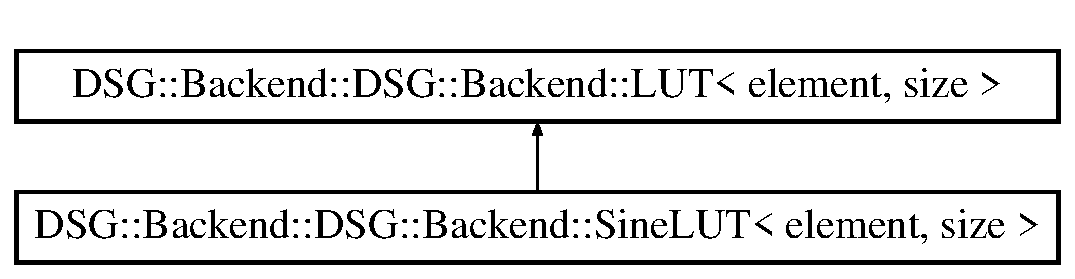
\includegraphics[height=2.000000cm]{classDSG_1_1Backend_1_1DSG_1_1Backend_1_1SineLUT}
\end{center}
\end{figure}
\subsection*{Public Member Functions}
\begin{DoxyCompactItemize}
\item 
\hyperlink{classDSG_1_1Backend_1_1DSG_1_1Backend_1_1SineLUT_a8efd77efae17db98591b2fa01962e234}{Sine\+L\+U\+T} ()
\item 
virtual \hyperlink{classDSG_1_1Backend_1_1DSG_1_1Backend_1_1SineLUT_af732d15e88429aeced938fe925624b3e}{$\sim$\+Sine\+L\+U\+T} ()
\item 
virtual element \hyperlink{classDSG_1_1Backend_1_1DSG_1_1Backend_1_1SineLUT_aaa841c0b14ec2a470d18932b816f78e6}{operator()} (double const \&x)
\item 
element const \& \hyperlink{classDSG_1_1Backend_1_1DSG_1_1Backend_1_1LUT_acd6db2fa4eba392de1cbb4795f351f8a}{operator\mbox{[}$\,$\mbox{]}} (unsigned long const \&index)
\item 
unsigned long const \& \hyperlink{classDSG_1_1Backend_1_1DSG_1_1Backend_1_1LUT_a65daa6f46f978a64da1c86089847602d}{Size} () const 
\end{DoxyCompactItemize}
\subsection*{Protected Attributes}
\begin{DoxyCompactItemize}
\item 
double \hyperlink{classDSG_1_1Backend_1_1DSG_1_1Backend_1_1SineLUT_a5ea74e278f77c7f0196fa642ccf45b40}{phs}
\item 
element \hyperlink{classDSG_1_1Backend_1_1DSG_1_1Backend_1_1LUT_a427da4b7eccdfe25e3c1889a8c2fdea6}{\+\_\+table} \mbox{[}size\mbox{]}
\item 
const unsigned long \hyperlink{classDSG_1_1Backend_1_1DSG_1_1Backend_1_1LUT_aa48956aa4debf08fdb517cb751d3e01d}{\+\_\+size}
\end{DoxyCompactItemize}


\subsection{Detailed Description}
\subsubsection*{template$<$typename element, unsigned long size$>$class D\+S\+G\+::\+Backend\+::\+D\+S\+G\+::\+Backend\+::\+Sine\+L\+U\+T$<$ element, size $>$}



Definition at line 21 of file Sin.\+h.



\subsection{Constructor \& Destructor Documentation}
\hypertarget{classDSG_1_1Backend_1_1DSG_1_1Backend_1_1SineLUT_a8efd77efae17db98591b2fa01962e234}{\index{D\+S\+G\+::\+Backend\+::\+D\+S\+G\+::\+Backend\+::\+Sine\+L\+U\+T@{D\+S\+G\+::\+Backend\+::\+D\+S\+G\+::\+Backend\+::\+Sine\+L\+U\+T}!Sine\+L\+U\+T@{Sine\+L\+U\+T}}
\index{Sine\+L\+U\+T@{Sine\+L\+U\+T}!D\+S\+G\+::\+Backend\+::\+D\+S\+G\+::\+Backend\+::\+Sine\+L\+U\+T@{D\+S\+G\+::\+Backend\+::\+D\+S\+G\+::\+Backend\+::\+Sine\+L\+U\+T}}
\subsubsection[{Sine\+L\+U\+T}]{\setlength{\rightskip}{0pt plus 5cm}template$<$typename element, unsigned long size$>$ {\bf D\+S\+G\+::\+Backend\+::\+D\+S\+G\+::\+Backend\+::\+Sine\+L\+U\+T}$<$ element, size $>$\+::{\bf Sine\+L\+U\+T} (
\begin{DoxyParamCaption}
{}
\end{DoxyParamCaption}
)\hspace{0.3cm}{\ttfamily [inline]}}}\label{classDSG_1_1Backend_1_1DSG_1_1Backend_1_1SineLUT_a8efd77efae17db98591b2fa01962e234}


Definition at line 23 of file Sin.\+h.


\begin{DoxyCode}
33                                         \{
\end{DoxyCode}
\hypertarget{classDSG_1_1Backend_1_1DSG_1_1Backend_1_1SineLUT_af732d15e88429aeced938fe925624b3e}{\index{D\+S\+G\+::\+Backend\+::\+D\+S\+G\+::\+Backend\+::\+Sine\+L\+U\+T@{D\+S\+G\+::\+Backend\+::\+D\+S\+G\+::\+Backend\+::\+Sine\+L\+U\+T}!````~Sine\+L\+U\+T@{$\sim$\+Sine\+L\+U\+T}}
\index{````~Sine\+L\+U\+T@{$\sim$\+Sine\+L\+U\+T}!D\+S\+G\+::\+Backend\+::\+D\+S\+G\+::\+Backend\+::\+Sine\+L\+U\+T@{D\+S\+G\+::\+Backend\+::\+D\+S\+G\+::\+Backend\+::\+Sine\+L\+U\+T}}
\subsubsection[{$\sim$\+Sine\+L\+U\+T}]{\setlength{\rightskip}{0pt plus 5cm}template$<$typename element, unsigned long size$>$ virtual {\bf D\+S\+G\+::\+Backend\+::\+D\+S\+G\+::\+Backend\+::\+Sine\+L\+U\+T}$<$ element, size $>$\+::$\sim${\bf Sine\+L\+U\+T} (
\begin{DoxyParamCaption}
{}
\end{DoxyParamCaption}
)\hspace{0.3cm}{\ttfamily [inline]}, {\ttfamily [virtual]}}}\label{classDSG_1_1Backend_1_1DSG_1_1Backend_1_1SineLUT_af732d15e88429aeced938fe925624b3e}


Definition at line 31 of file Sin.\+h.


\begin{DoxyCode}
33 \{
\end{DoxyCode}


\subsection{Member Function Documentation}
\hypertarget{classDSG_1_1Backend_1_1DSG_1_1Backend_1_1SineLUT_aaa841c0b14ec2a470d18932b816f78e6}{\index{D\+S\+G\+::\+Backend\+::\+D\+S\+G\+::\+Backend\+::\+Sine\+L\+U\+T@{D\+S\+G\+::\+Backend\+::\+D\+S\+G\+::\+Backend\+::\+Sine\+L\+U\+T}!operator()@{operator()}}
\index{operator()@{operator()}!D\+S\+G\+::\+Backend\+::\+D\+S\+G\+::\+Backend\+::\+Sine\+L\+U\+T@{D\+S\+G\+::\+Backend\+::\+D\+S\+G\+::\+Backend\+::\+Sine\+L\+U\+T}}
\subsubsection[{operator()}]{\setlength{\rightskip}{0pt plus 5cm}template$<$typename element, unsigned long size$>$ virtual element {\bf D\+S\+G\+::\+Backend\+::\+D\+S\+G\+::\+Backend\+::\+Sine\+L\+U\+T}$<$ element, size $>$\+::operator() (
\begin{DoxyParamCaption}
\item[{double const \&}]{x}
\end{DoxyParamCaption}
)\hspace{0.3cm}{\ttfamily [inline]}, {\ttfamily [virtual]}}}\label{classDSG_1_1Backend_1_1DSG_1_1Backend_1_1SineLUT_aaa841c0b14ec2a470d18932b816f78e6}


Reimplemented from \hyperlink{classDSG_1_1Backend_1_1DSG_1_1Backend_1_1LUT_a4cdb48ce3c472160931968739623f8ac}{D\+S\+G\+::\+Backend\+::\+D\+S\+G\+::\+Backend\+::\+L\+U\+T$<$ element, size $>$}.



Definition at line 32 of file Sin.\+h.


\begin{DoxyCode}
33                                         \{
34         \textcolor{comment}{//phs 0-1}
35 \textcolor{preprocessor}{#if sin\_impl == sin\_native}
36         \textcolor{keywordflow}{return} sin(\hyperlink{Sin_8h_a4912c64aec0c943b7985db6cb61ff83a}{TWOPI} * \hyperlink{classDSG_1_1Backend_1_1DSG_1_1Backend_1_1SineLUT_a5ea74e278f77c7f0196fa642ccf45b40}{phs});
37 \textcolor{preprocessor}{#elif sin\_impl == sin\_tay}
38         \textcolor{keywordflow}{return} \hyperlink{namespaceDSG_1_1Backend_1_1Taylor_ad36e85fc2ea4a8b773371dd7b92fdb92}{Taylor::Sine}(\hyperlink{classDSG_1_1Backend_1_1DSG_1_1Backend_1_1SineLUT_a5ea74e278f77c7f0196fa642ccf45b40}{phs}*\hyperlink{Sin_8h_a4912c64aec0c943b7985db6cb61ff83a}{TWOPI});
39 \textcolor{preprocessor}{#elif sin\_impl == sin\_lut}
40         \textcolor{keyword}{static} \hyperlink{classDSG_1_1Backend_1_1SineLUT}{DSG::Backend::SineLUT<float, 32768>} sine;
\end{DoxyCode}
\hypertarget{classDSG_1_1Backend_1_1DSG_1_1Backend_1_1LUT_acd6db2fa4eba392de1cbb4795f351f8a}{\index{D\+S\+G\+::\+Backend\+::\+D\+S\+G\+::\+Backend\+::\+Sine\+L\+U\+T@{D\+S\+G\+::\+Backend\+::\+D\+S\+G\+::\+Backend\+::\+Sine\+L\+U\+T}!operator\mbox{[}$\,$\mbox{]}@{operator[]}}
\index{operator\mbox{[}$\,$\mbox{]}@{operator[]}!D\+S\+G\+::\+Backend\+::\+D\+S\+G\+::\+Backend\+::\+Sine\+L\+U\+T@{D\+S\+G\+::\+Backend\+::\+D\+S\+G\+::\+Backend\+::\+Sine\+L\+U\+T}}
\subsubsection[{operator[]}]{\setlength{\rightskip}{0pt plus 5cm}template$<$typename element, unsigned long size$>$ element const\& {\bf D\+S\+G\+::\+Backend\+::\+D\+S\+G\+::\+Backend\+::\+L\+U\+T}$<$ element, size $>$\+::operator\mbox{[}$\,$\mbox{]} (
\begin{DoxyParamCaption}
\item[{unsigned long const \&}]{index}
\end{DoxyParamCaption}
)\hspace{0.3cm}{\ttfamily [inline]}, {\ttfamily [inherited]}}}\label{classDSG_1_1Backend_1_1DSG_1_1Backend_1_1LUT_acd6db2fa4eba392de1cbb4795f351f8a}


Definition at line 24 of file Sin.\+h.


\begin{DoxyCode}
33                                         \{
\end{DoxyCode}
\hypertarget{classDSG_1_1Backend_1_1DSG_1_1Backend_1_1LUT_a65daa6f46f978a64da1c86089847602d}{\index{D\+S\+G\+::\+Backend\+::\+D\+S\+G\+::\+Backend\+::\+Sine\+L\+U\+T@{D\+S\+G\+::\+Backend\+::\+D\+S\+G\+::\+Backend\+::\+Sine\+L\+U\+T}!Size@{Size}}
\index{Size@{Size}!D\+S\+G\+::\+Backend\+::\+D\+S\+G\+::\+Backend\+::\+Sine\+L\+U\+T@{D\+S\+G\+::\+Backend\+::\+D\+S\+G\+::\+Backend\+::\+Sine\+L\+U\+T}}
\subsubsection[{Size}]{\setlength{\rightskip}{0pt plus 5cm}template$<$typename element, unsigned long size$>$ unsigned long const\& {\bf D\+S\+G\+::\+Backend\+::\+D\+S\+G\+::\+Backend\+::\+L\+U\+T}$<$ element, size $>$\+::Size (
\begin{DoxyParamCaption}
{}
\end{DoxyParamCaption}
) const\hspace{0.3cm}{\ttfamily [inline]}, {\ttfamily [inherited]}}}\label{classDSG_1_1Backend_1_1DSG_1_1Backend_1_1LUT_a65daa6f46f978a64da1c86089847602d}


Definition at line 33 of file Sin.\+h.


\begin{DoxyCode}
33                                         \{
34         \textcolor{comment}{//phs 0-1}
35 \textcolor{preprocessor}{#if sin\_impl == sin\_native}
\end{DoxyCode}


\subsection{Member Data Documentation}
\hypertarget{classDSG_1_1Backend_1_1DSG_1_1Backend_1_1LUT_aa48956aa4debf08fdb517cb751d3e01d}{\index{D\+S\+G\+::\+Backend\+::\+D\+S\+G\+::\+Backend\+::\+Sine\+L\+U\+T@{D\+S\+G\+::\+Backend\+::\+D\+S\+G\+::\+Backend\+::\+Sine\+L\+U\+T}!\+\_\+size@{\+\_\+size}}
\index{\+\_\+size@{\+\_\+size}!D\+S\+G\+::\+Backend\+::\+D\+S\+G\+::\+Backend\+::\+Sine\+L\+U\+T@{D\+S\+G\+::\+Backend\+::\+D\+S\+G\+::\+Backend\+::\+Sine\+L\+U\+T}}
\subsubsection[{\+\_\+size}]{\setlength{\rightskip}{0pt plus 5cm}template$<$typename element, unsigned long size$>$ const unsigned long {\bf D\+S\+G\+::\+Backend\+::\+D\+S\+G\+::\+Backend\+::\+L\+U\+T}$<$ element, size $>$\+::\+\_\+size\hspace{0.3cm}{\ttfamily [protected]}, {\ttfamily [inherited]}}}\label{classDSG_1_1Backend_1_1DSG_1_1Backend_1_1LUT_aa48956aa4debf08fdb517cb751d3e01d}


Definition at line 38 of file Sin.\+h.

\hypertarget{classDSG_1_1Backend_1_1DSG_1_1Backend_1_1LUT_a427da4b7eccdfe25e3c1889a8c2fdea6}{\index{D\+S\+G\+::\+Backend\+::\+D\+S\+G\+::\+Backend\+::\+Sine\+L\+U\+T@{D\+S\+G\+::\+Backend\+::\+D\+S\+G\+::\+Backend\+::\+Sine\+L\+U\+T}!\+\_\+table@{\+\_\+table}}
\index{\+\_\+table@{\+\_\+table}!D\+S\+G\+::\+Backend\+::\+D\+S\+G\+::\+Backend\+::\+Sine\+L\+U\+T@{D\+S\+G\+::\+Backend\+::\+D\+S\+G\+::\+Backend\+::\+Sine\+L\+U\+T}}
\subsubsection[{\+\_\+table}]{\setlength{\rightskip}{0pt plus 5cm}template$<$typename element, unsigned long size$>$ element {\bf D\+S\+G\+::\+Backend\+::\+D\+S\+G\+::\+Backend\+::\+L\+U\+T}$<$ element, size $>$\+::\+\_\+table\mbox{[}size\mbox{]}\hspace{0.3cm}{\ttfamily [protected]}, {\ttfamily [inherited]}}}\label{classDSG_1_1Backend_1_1DSG_1_1Backend_1_1LUT_a427da4b7eccdfe25e3c1889a8c2fdea6}


Definition at line 37 of file Sin.\+h.

\hypertarget{classDSG_1_1Backend_1_1DSG_1_1Backend_1_1SineLUT_a5ea74e278f77c7f0196fa642ccf45b40}{\index{D\+S\+G\+::\+Backend\+::\+D\+S\+G\+::\+Backend\+::\+Sine\+L\+U\+T@{D\+S\+G\+::\+Backend\+::\+D\+S\+G\+::\+Backend\+::\+Sine\+L\+U\+T}!phs@{phs}}
\index{phs@{phs}!D\+S\+G\+::\+Backend\+::\+D\+S\+G\+::\+Backend\+::\+Sine\+L\+U\+T@{D\+S\+G\+::\+Backend\+::\+D\+S\+G\+::\+Backend\+::\+Sine\+L\+U\+T}}
\subsubsection[{phs}]{\setlength{\rightskip}{0pt plus 5cm}template$<$typename element, unsigned long size$>$ double {\bf D\+S\+G\+::\+Backend\+::\+D\+S\+G\+::\+Backend\+::\+Sine\+L\+U\+T}$<$ element, size $>$\+::phs\hspace{0.3cm}{\ttfamily [protected]}}}\label{classDSG_1_1Backend_1_1DSG_1_1Backend_1_1SineLUT_a5ea74e278f77c7f0196fa642ccf45b40}


Definition at line 42 of file Sin.\+h.



The documentation for this class was generated from the following file\+:\begin{DoxyCompactItemize}
\item 
/\+Users/alexanderzywicki/\+Documents/\+School\+\_\+\+Stuff/\+Fall\+\_\+2014/\+Digital\+\_\+\+Signal\+\_\+\+Generation\+\_\+and\+\_\+\+Analysis/src/include/\hyperlink{Sin_8h}{Sin.\+h}\end{DoxyCompactItemize}

\hypertarget{classDSG_1_1Backend_1_1SineLUT}{\section{D\+S\+G\+:\+:Backend\+:\+:Sine\+L\+U\+T$<$ element, size $>$ Class Template Reference}
\label{classDSG_1_1Backend_1_1SineLUT}\index{D\+S\+G\+::\+Backend\+::\+Sine\+L\+U\+T$<$ element, size $>$@{D\+S\+G\+::\+Backend\+::\+Sine\+L\+U\+T$<$ element, size $>$}}
}


{\ttfamily \#include $<$Sine\+L\+U\+T.\+h$>$}

Inheritance diagram for D\+S\+G\+:\+:Backend\+:\+:Sine\+L\+U\+T$<$ element, size $>$\+:\begin{figure}[H]
\begin{center}
\leavevmode
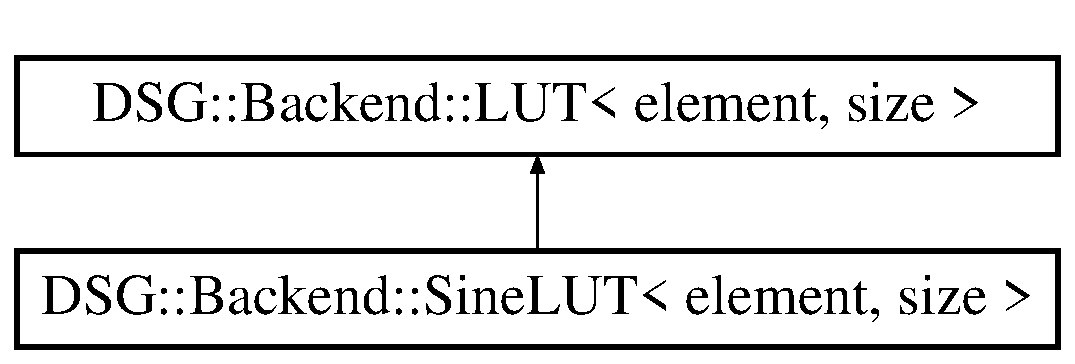
\includegraphics[height=2.000000cm]{classDSG_1_1Backend_1_1SineLUT}
\end{center}
\end{figure}
\subsection*{Public Member Functions}
\begin{DoxyCompactItemize}
\item 
\hyperlink{classDSG_1_1Backend_1_1SineLUT_a9da7b21af95cd94c4f7b9bd6b71cbb70}{Sine\+L\+U\+T} ()
\item 
virtual \hyperlink{classDSG_1_1Backend_1_1SineLUT_af910f9329f237b770c6b409b598fe5c9}{$\sim$\+Sine\+L\+U\+T} ()
\item 
virtual element const \& \hyperlink{classDSG_1_1Backend_1_1SineLUT_a52f73d7656d11c5cc0b6e937dbd8e2b8}{operator()} (double const \&x)
\item 
element const \& \hyperlink{classDSG_1_1Backend_1_1LUT_a50d8304c33760ed566039ebf5657807c}{operator\mbox{[}$\,$\mbox{]}} (unsigned long const \&index)
\item 
unsigned long const \& \hyperlink{classDSG_1_1Backend_1_1LUT_a988c07b5002e0aee6e490244b80c8830}{Size} () const 
\end{DoxyCompactItemize}
\subsection*{Protected Attributes}
\begin{DoxyCompactItemize}
\item 
double \hyperlink{classDSG_1_1Backend_1_1SineLUT_a4745a2ef3a5cec8f2822fa12174e059b}{phs}
\item 
element \hyperlink{classDSG_1_1Backend_1_1LUT_a23615428e84d6be4424c8b897866f253}{\+\_\+table} \mbox{[}size\mbox{]}
\item 
const unsigned long \hyperlink{classDSG_1_1Backend_1_1LUT_ae18fa23936c51c1bdbd21311c9f1054e}{\+\_\+size}
\end{DoxyCompactItemize}


\subsection{Detailed Description}
\subsubsection*{template$<$typename element, unsigned long size$>$class D\+S\+G\+::\+Backend\+::\+Sine\+L\+U\+T$<$ element, size $>$}



Definition at line 19 of file Sine\+L\+U\+T.\+h.



\subsection{Constructor \& Destructor Documentation}
\hypertarget{classDSG_1_1Backend_1_1SineLUT_a9da7b21af95cd94c4f7b9bd6b71cbb70}{\index{D\+S\+G\+::\+Backend\+::\+Sine\+L\+U\+T@{D\+S\+G\+::\+Backend\+::\+Sine\+L\+U\+T}!Sine\+L\+U\+T@{Sine\+L\+U\+T}}
\index{Sine\+L\+U\+T@{Sine\+L\+U\+T}!D\+S\+G\+::\+Backend\+::\+Sine\+L\+U\+T@{D\+S\+G\+::\+Backend\+::\+Sine\+L\+U\+T}}
\subsubsection[{Sine\+L\+U\+T}]{\setlength{\rightskip}{0pt plus 5cm}template$<$typename element, unsigned long size$>$ {\bf D\+S\+G\+::\+Backend\+::\+Sine\+L\+U\+T}$<$ element, size $>$\+::{\bf Sine\+L\+U\+T} (
\begin{DoxyParamCaption}
{}
\end{DoxyParamCaption}
)\hspace{0.3cm}{\ttfamily [inline]}}}\label{classDSG_1_1Backend_1_1SineLUT_a9da7b21af95cd94c4f7b9bd6b71cbb70}


Definition at line 21 of file Sine\+L\+U\+T.\+h.


\begin{DoxyCode}
21                      :LUT<element,size>()\{
22                 \textcolor{keywordtype}{double} step = (\hyperlink{PI_8h_a4912c64aec0c943b7985db6cb61ff83a}{TWOPI}/this->\hyperlink{classDSG_1_1Backend_1_1LUT_ae18fa23936c51c1bdbd21311c9f1054e}{\_size});
23                 \textcolor{keywordtype}{double} \hyperlink{classDSG_1_1Backend_1_1SineLUT_a4745a2ef3a5cec8f2822fa12174e059b}{phs}=0;
24                 \textcolor{keywordflow}{for} (\textcolor{keywordtype}{int} i=0; i<this->\hyperlink{classDSG_1_1Backend_1_1LUT_ae18fa23936c51c1bdbd21311c9f1054e}{\_size}; ++i) \{
25                     this->\hyperlink{classDSG_1_1Backend_1_1LUT_a23615428e84d6be4424c8b897866f253}{\_table}[i] = sin(phs);
26                     phs+=step;
27                 \}
28             \}
\end{DoxyCode}
\hypertarget{classDSG_1_1Backend_1_1SineLUT_af910f9329f237b770c6b409b598fe5c9}{\index{D\+S\+G\+::\+Backend\+::\+Sine\+L\+U\+T@{D\+S\+G\+::\+Backend\+::\+Sine\+L\+U\+T}!````~Sine\+L\+U\+T@{$\sim$\+Sine\+L\+U\+T}}
\index{````~Sine\+L\+U\+T@{$\sim$\+Sine\+L\+U\+T}!D\+S\+G\+::\+Backend\+::\+Sine\+L\+U\+T@{D\+S\+G\+::\+Backend\+::\+Sine\+L\+U\+T}}
\subsubsection[{$\sim$\+Sine\+L\+U\+T}]{\setlength{\rightskip}{0pt plus 5cm}template$<$typename element, unsigned long size$>$ virtual {\bf D\+S\+G\+::\+Backend\+::\+Sine\+L\+U\+T}$<$ element, size $>$\+::$\sim${\bf Sine\+L\+U\+T} (
\begin{DoxyParamCaption}
{}
\end{DoxyParamCaption}
)\hspace{0.3cm}{\ttfamily [inline]}, {\ttfamily [virtual]}}}\label{classDSG_1_1Backend_1_1SineLUT_af910f9329f237b770c6b409b598fe5c9}


Definition at line 29 of file Sine\+L\+U\+T.\+h.


\begin{DoxyCode}
29 \{\}
\end{DoxyCode}


\subsection{Member Function Documentation}
\hypertarget{classDSG_1_1Backend_1_1SineLUT_a52f73d7656d11c5cc0b6e937dbd8e2b8}{\index{D\+S\+G\+::\+Backend\+::\+Sine\+L\+U\+T@{D\+S\+G\+::\+Backend\+::\+Sine\+L\+U\+T}!operator()@{operator()}}
\index{operator()@{operator()}!D\+S\+G\+::\+Backend\+::\+Sine\+L\+U\+T@{D\+S\+G\+::\+Backend\+::\+Sine\+L\+U\+T}}
\subsubsection[{operator()}]{\setlength{\rightskip}{0pt plus 5cm}template$<$typename element, unsigned long size$>$ virtual element const\& {\bf D\+S\+G\+::\+Backend\+::\+Sine\+L\+U\+T}$<$ element, size $>$\+::operator() (
\begin{DoxyParamCaption}
\item[{double const \&}]{x}
\end{DoxyParamCaption}
)\hspace{0.3cm}{\ttfamily [inline]}, {\ttfamily [virtual]}}}\label{classDSG_1_1Backend_1_1SineLUT_a52f73d7656d11c5cc0b6e937dbd8e2b8}


Reimplemented from \hyperlink{classDSG_1_1Backend_1_1LUT_aa31a17b115eebb9a2a9ad45b32c8d26a}{D\+S\+G\+::\+Backend\+::\+L\+U\+T$<$ element, size $>$}.



Definition at line 30 of file Sine\+L\+U\+T.\+h.


\begin{DoxyCode}
30                                                                      \{
31                 \hyperlink{classDSG_1_1Backend_1_1SineLUT_a4745a2ef3a5cec8f2822fa12174e059b}{phs}=x;
32                 \textcolor{comment}{//need range checking on x to ensure 0-1 range}
33                 \hyperlink{classDSG_1_1Backend_1_1SineLUT_a4745a2ef3a5cec8f2822fa12174e059b}{phs}<0 ? \hyperlink{classDSG_1_1Backend_1_1SineLUT_a4745a2ef3a5cec8f2822fa12174e059b}{phs} = 1-(phs*-1):0;
34                 phs-=((int)phs);
35                 \textcolor{keywordflow}{return} this->\hyperlink{classDSG_1_1Backend_1_1LUT_a23615428e84d6be4424c8b897866f253}{\_table}[(unsigned)(phs* (this->\hyperlink{classDSG_1_1Backend_1_1LUT_ae18fa23936c51c1bdbd21311c9f1054e}{\_size}-1))];
36             \}
\end{DoxyCode}
\hypertarget{classDSG_1_1Backend_1_1LUT_a50d8304c33760ed566039ebf5657807c}{\index{D\+S\+G\+::\+Backend\+::\+Sine\+L\+U\+T@{D\+S\+G\+::\+Backend\+::\+Sine\+L\+U\+T}!operator\mbox{[}$\,$\mbox{]}@{operator[]}}
\index{operator\mbox{[}$\,$\mbox{]}@{operator[]}!D\+S\+G\+::\+Backend\+::\+Sine\+L\+U\+T@{D\+S\+G\+::\+Backend\+::\+Sine\+L\+U\+T}}
\subsubsection[{operator[]}]{\setlength{\rightskip}{0pt plus 5cm}template$<$typename element, unsigned long size$>$ element const\& {\bf D\+S\+G\+::\+Backend\+::\+L\+U\+T}$<$ element, size $>$\+::operator\mbox{[}$\,$\mbox{]} (
\begin{DoxyParamCaption}
\item[{unsigned long const \&}]{index}
\end{DoxyParamCaption}
)\hspace{0.3cm}{\ttfamily [inline]}, {\ttfamily [inherited]}}}\label{classDSG_1_1Backend_1_1LUT_a50d8304c33760ed566039ebf5657807c}


Definition at line 22 of file L\+U\+T.\+h.


\begin{DoxyCode}
22                                                                  \{
23 \textcolor{preprocessor}{#ifdef DEBUG}
24                 assert(index<\hyperlink{classDSG_1_1Backend_1_1LUT_ae18fa23936c51c1bdbd21311c9f1054e}{\_size});
25 \textcolor{preprocessor}{#endif}
26                 \textcolor{keywordflow}{return} \hyperlink{classDSG_1_1Backend_1_1LUT_a23615428e84d6be4424c8b897866f253}{\_table}[index];
27             \}
\end{DoxyCode}
\hypertarget{classDSG_1_1Backend_1_1LUT_a988c07b5002e0aee6e490244b80c8830}{\index{D\+S\+G\+::\+Backend\+::\+Sine\+L\+U\+T@{D\+S\+G\+::\+Backend\+::\+Sine\+L\+U\+T}!Size@{Size}}
\index{Size@{Size}!D\+S\+G\+::\+Backend\+::\+Sine\+L\+U\+T@{D\+S\+G\+::\+Backend\+::\+Sine\+L\+U\+T}}
\subsubsection[{Size}]{\setlength{\rightskip}{0pt plus 5cm}template$<$typename element, unsigned long size$>$ unsigned long const\& {\bf D\+S\+G\+::\+Backend\+::\+L\+U\+T}$<$ element, size $>$\+::Size (
\begin{DoxyParamCaption}
{}
\end{DoxyParamCaption}
) const\hspace{0.3cm}{\ttfamily [inline]}, {\ttfamily [inherited]}}}\label{classDSG_1_1Backend_1_1LUT_a988c07b5002e0aee6e490244b80c8830}


Definition at line 31 of file L\+U\+T.\+h.


\begin{DoxyCode}
31                                             \{
32                 \textcolor{keywordflow}{return} \hyperlink{classDSG_1_1Backend_1_1LUT_ae18fa23936c51c1bdbd21311c9f1054e}{\_size};
33             \}
\end{DoxyCode}


\subsection{Member Data Documentation}
\hypertarget{classDSG_1_1Backend_1_1LUT_ae18fa23936c51c1bdbd21311c9f1054e}{\index{D\+S\+G\+::\+Backend\+::\+Sine\+L\+U\+T@{D\+S\+G\+::\+Backend\+::\+Sine\+L\+U\+T}!\+\_\+size@{\+\_\+size}}
\index{\+\_\+size@{\+\_\+size}!D\+S\+G\+::\+Backend\+::\+Sine\+L\+U\+T@{D\+S\+G\+::\+Backend\+::\+Sine\+L\+U\+T}}
\subsubsection[{\+\_\+size}]{\setlength{\rightskip}{0pt plus 5cm}template$<$typename element, unsigned long size$>$ const unsigned long {\bf D\+S\+G\+::\+Backend\+::\+L\+U\+T}$<$ element, size $>$\+::\+\_\+size\hspace{0.3cm}{\ttfamily [protected]}, {\ttfamily [inherited]}}}\label{classDSG_1_1Backend_1_1LUT_ae18fa23936c51c1bdbd21311c9f1054e}


Definition at line 36 of file L\+U\+T.\+h.

\hypertarget{classDSG_1_1Backend_1_1LUT_a23615428e84d6be4424c8b897866f253}{\index{D\+S\+G\+::\+Backend\+::\+Sine\+L\+U\+T@{D\+S\+G\+::\+Backend\+::\+Sine\+L\+U\+T}!\+\_\+table@{\+\_\+table}}
\index{\+\_\+table@{\+\_\+table}!D\+S\+G\+::\+Backend\+::\+Sine\+L\+U\+T@{D\+S\+G\+::\+Backend\+::\+Sine\+L\+U\+T}}
\subsubsection[{\+\_\+table}]{\setlength{\rightskip}{0pt plus 5cm}template$<$typename element, unsigned long size$>$ element {\bf D\+S\+G\+::\+Backend\+::\+L\+U\+T}$<$ element, size $>$\+::\+\_\+table\mbox{[}size\mbox{]}\hspace{0.3cm}{\ttfamily [protected]}, {\ttfamily [inherited]}}}\label{classDSG_1_1Backend_1_1LUT_a23615428e84d6be4424c8b897866f253}


Definition at line 35 of file L\+U\+T.\+h.

\hypertarget{classDSG_1_1Backend_1_1SineLUT_a4745a2ef3a5cec8f2822fa12174e059b}{\index{D\+S\+G\+::\+Backend\+::\+Sine\+L\+U\+T@{D\+S\+G\+::\+Backend\+::\+Sine\+L\+U\+T}!phs@{phs}}
\index{phs@{phs}!D\+S\+G\+::\+Backend\+::\+Sine\+L\+U\+T@{D\+S\+G\+::\+Backend\+::\+Sine\+L\+U\+T}}
\subsubsection[{phs}]{\setlength{\rightskip}{0pt plus 5cm}template$<$typename element, unsigned long size$>$ double {\bf D\+S\+G\+::\+Backend\+::\+Sine\+L\+U\+T}$<$ element, size $>$\+::phs\hspace{0.3cm}{\ttfamily [protected]}}}\label{classDSG_1_1Backend_1_1SineLUT_a4745a2ef3a5cec8f2822fa12174e059b}


Definition at line 38 of file Sine\+L\+U\+T.\+h.



The documentation for this class was generated from the following file\+:\begin{DoxyCompactItemize}
\item 
/\+Users/alexanderzywicki/\+Documents/\+School\+\_\+\+Stuff/\+Fall\+\_\+2014/\+Digital\+\_\+\+Signal\+\_\+\+Generation\+\_\+and\+\_\+\+Analysis/src/include/\hyperlink{SineLUT_8h}{Sine\+L\+U\+T.\+h}\end{DoxyCompactItemize}

\hypertarget{classDSG_1_1Backend_1_1SmallSineLUT}{\section{D\+S\+G\+:\+:Backend\+:\+:Small\+Sine\+L\+U\+T$<$ element, size $>$ Class Template Reference}
\label{classDSG_1_1Backend_1_1SmallSineLUT}\index{D\+S\+G\+::\+Backend\+::\+Small\+Sine\+L\+U\+T$<$ element, size $>$@{D\+S\+G\+::\+Backend\+::\+Small\+Sine\+L\+U\+T$<$ element, size $>$}}
}


{\ttfamily \#include $<$Sine\+L\+U\+T.\+h$>$}

Inheritance diagram for D\+S\+G\+:\+:Backend\+:\+:Small\+Sine\+L\+U\+T$<$ element, size $>$\+:\begin{figure}[H]
\begin{center}
\leavevmode
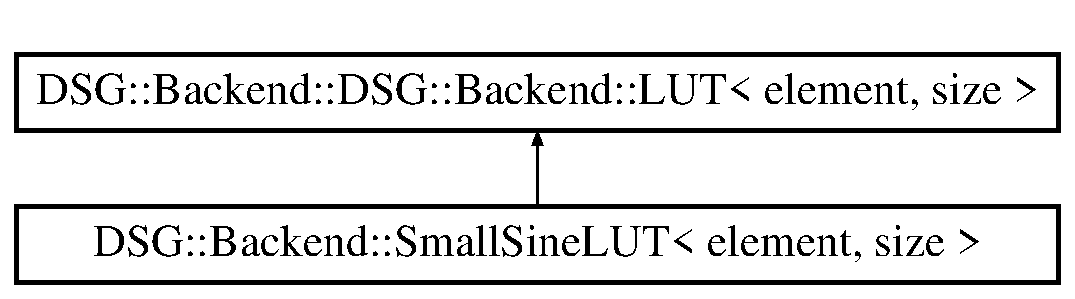
\includegraphics[height=2.000000cm]{classDSG_1_1Backend_1_1SmallSineLUT}
\end{center}
\end{figure}
\subsection*{Public Member Functions}
\begin{DoxyCompactItemize}
\item 
\hyperlink{classDSG_1_1Backend_1_1SmallSineLUT_a2c6aac15943d6373b108336efd29cc03}{Small\+Sine\+L\+U\+T} ()
\item 
virtual \hyperlink{classDSG_1_1Backend_1_1SmallSineLUT_aa94632e333017986bb58b14a5480da52}{$\sim$\+Small\+Sine\+L\+U\+T} ()
\item 
virtual element \hyperlink{classDSG_1_1Backend_1_1SmallSineLUT_af4b947cb0760ade07b788dae2472f4c0}{operator()} (double const \&x)
\item 
element const \& \hyperlink{classDSG_1_1Backend_1_1LUT_a50d8304c33760ed566039ebf5657807c}{operator\mbox{[}$\,$\mbox{]}} (unsigned long const \&index)
\item 
unsigned long const \& \hyperlink{classDSG_1_1Backend_1_1LUT_a988c07b5002e0aee6e490244b80c8830}{Size} () const 
\end{DoxyCompactItemize}
\subsection*{Protected Member Functions}
\begin{DoxyCompactItemize}
\item 
void \hyperlink{classDSG_1_1Backend_1_1SmallSineLUT_a97ffb8a84efa321e6f2733e17205113a}{fill} ()
\item 
element const \& \hyperlink{classDSG_1_1Backend_1_1SmallSineLUT_a1af95a7037c3abacf58700975deecb3a}{lookup} (double index)
\end{DoxyCompactItemize}
\subsection*{Protected Attributes}
\begin{DoxyCompactItemize}
\item 
element \hyperlink{classDSG_1_1Backend_1_1LUT_a23615428e84d6be4424c8b897866f253}{\+\_\+table} \mbox{[}size\mbox{]}
\item 
const unsigned long \hyperlink{classDSG_1_1Backend_1_1LUT_ae18fa23936c51c1bdbd21311c9f1054e}{\+\_\+size}
\end{DoxyCompactItemize}


\subsection{Detailed Description}
\subsubsection*{template$<$typename element, unsigned long size$>$class D\+S\+G\+::\+Backend\+::\+Small\+Sine\+L\+U\+T$<$ element, size $>$}



Definition at line 41 of file Sine\+L\+U\+T.\+h.



\subsection{Constructor \& Destructor Documentation}
\hypertarget{classDSG_1_1Backend_1_1SmallSineLUT_a2c6aac15943d6373b108336efd29cc03}{\index{D\+S\+G\+::\+Backend\+::\+Small\+Sine\+L\+U\+T@{D\+S\+G\+::\+Backend\+::\+Small\+Sine\+L\+U\+T}!Small\+Sine\+L\+U\+T@{Small\+Sine\+L\+U\+T}}
\index{Small\+Sine\+L\+U\+T@{Small\+Sine\+L\+U\+T}!D\+S\+G\+::\+Backend\+::\+Small\+Sine\+L\+U\+T@{D\+S\+G\+::\+Backend\+::\+Small\+Sine\+L\+U\+T}}
\subsubsection[{Small\+Sine\+L\+U\+T}]{\setlength{\rightskip}{0pt plus 5cm}template$<$typename element , unsigned long size$>$ {\bf D\+S\+G\+::\+Backend\+::\+Small\+Sine\+L\+U\+T}$<$ element, size $>$\+::{\bf Small\+Sine\+L\+U\+T} (
\begin{DoxyParamCaption}
{}
\end{DoxyParamCaption}
)\hspace{0.3cm}{\ttfamily [inline]}}}\label{classDSG_1_1Backend_1_1SmallSineLUT_a2c6aac15943d6373b108336efd29cc03}


Definition at line 43 of file Sine\+L\+U\+T.\+h.


\begin{DoxyCode}
43 :LUT<element,size>()\{\hyperlink{classDSG_1_1Backend_1_1SmallSineLUT_a97ffb8a84efa321e6f2733e17205113a}{fill}();\}
\end{DoxyCode}
\hypertarget{classDSG_1_1Backend_1_1SmallSineLUT_aa94632e333017986bb58b14a5480da52}{\index{D\+S\+G\+::\+Backend\+::\+Small\+Sine\+L\+U\+T@{D\+S\+G\+::\+Backend\+::\+Small\+Sine\+L\+U\+T}!````~Small\+Sine\+L\+U\+T@{$\sim$\+Small\+Sine\+L\+U\+T}}
\index{````~Small\+Sine\+L\+U\+T@{$\sim$\+Small\+Sine\+L\+U\+T}!D\+S\+G\+::\+Backend\+::\+Small\+Sine\+L\+U\+T@{D\+S\+G\+::\+Backend\+::\+Small\+Sine\+L\+U\+T}}
\subsubsection[{$\sim$\+Small\+Sine\+L\+U\+T}]{\setlength{\rightskip}{0pt plus 5cm}template$<$typename element , unsigned long size$>$ virtual {\bf D\+S\+G\+::\+Backend\+::\+Small\+Sine\+L\+U\+T}$<$ element, size $>$\+::$\sim${\bf Small\+Sine\+L\+U\+T} (
\begin{DoxyParamCaption}
{}
\end{DoxyParamCaption}
)\hspace{0.3cm}{\ttfamily [inline]}, {\ttfamily [virtual]}}}\label{classDSG_1_1Backend_1_1SmallSineLUT_aa94632e333017986bb58b14a5480da52}


Definition at line 44 of file Sine\+L\+U\+T.\+h.


\begin{DoxyCode}
44 \{\}
\end{DoxyCode}


\subsection{Member Function Documentation}
\hypertarget{classDSG_1_1Backend_1_1SmallSineLUT_a97ffb8a84efa321e6f2733e17205113a}{\index{D\+S\+G\+::\+Backend\+::\+Small\+Sine\+L\+U\+T@{D\+S\+G\+::\+Backend\+::\+Small\+Sine\+L\+U\+T}!fill@{fill}}
\index{fill@{fill}!D\+S\+G\+::\+Backend\+::\+Small\+Sine\+L\+U\+T@{D\+S\+G\+::\+Backend\+::\+Small\+Sine\+L\+U\+T}}
\subsubsection[{fill}]{\setlength{\rightskip}{0pt plus 5cm}template$<$typename element , unsigned long size$>$ void {\bf D\+S\+G\+::\+Backend\+::\+Small\+Sine\+L\+U\+T}$<$ element, size $>$\+::fill (
\begin{DoxyParamCaption}
{}
\end{DoxyParamCaption}
)\hspace{0.3cm}{\ttfamily [inline]}, {\ttfamily [protected]}}}\label{classDSG_1_1Backend_1_1SmallSineLUT_a97ffb8a84efa321e6f2733e17205113a}


Definition at line 66 of file Sine\+L\+U\+T.\+h.


\begin{DoxyCode}
66                               \{
67                 \textcolor{keywordtype}{double} step = (M\_PI\_2/this->\hyperlink{classDSG_1_1Backend_1_1LUT_ae18fa23936c51c1bdbd21311c9f1054e}{\_size});
68                 \textcolor{keywordtype}{double} phs=0;
69                 \textcolor{keywordflow}{for} (\textcolor{keywordtype}{int} i=0; i<this->\hyperlink{classDSG_1_1Backend_1_1LUT_ae18fa23936c51c1bdbd21311c9f1054e}{\_size}; ++i) \{
70                     this->\hyperlink{classDSG_1_1Backend_1_1LUT_a23615428e84d6be4424c8b897866f253}{\_table}[i] = sin(phs);
71                     phs+=step;
72                 \}
73             \}
\end{DoxyCode}
\hypertarget{classDSG_1_1Backend_1_1SmallSineLUT_a1af95a7037c3abacf58700975deecb3a}{\index{D\+S\+G\+::\+Backend\+::\+Small\+Sine\+L\+U\+T@{D\+S\+G\+::\+Backend\+::\+Small\+Sine\+L\+U\+T}!lookup@{lookup}}
\index{lookup@{lookup}!D\+S\+G\+::\+Backend\+::\+Small\+Sine\+L\+U\+T@{D\+S\+G\+::\+Backend\+::\+Small\+Sine\+L\+U\+T}}
\subsubsection[{lookup}]{\setlength{\rightskip}{0pt plus 5cm}template$<$typename element , unsigned long size$>$ element const\& {\bf D\+S\+G\+::\+Backend\+::\+Small\+Sine\+L\+U\+T}$<$ element, size $>$\+::lookup (
\begin{DoxyParamCaption}
\item[{double}]{index}
\end{DoxyParamCaption}
)\hspace{0.3cm}{\ttfamily [inline]}, {\ttfamily [protected]}}}\label{classDSG_1_1Backend_1_1SmallSineLUT_a1af95a7037c3abacf58700975deecb3a}


Definition at line 74 of file Sine\+L\+U\+T.\+h.


\begin{DoxyCode}
74                                                       \{
75                 \textcolor{comment}{//possibvly interpolate for better quality}
76                 \textcolor{keywordflow}{return} this->\hyperlink{classDSG_1_1Backend_1_1LUT_a23615428e84d6be4424c8b897866f253}{\_table}[(unsigned)(index* (this->\hyperlink{classDSG_1_1Backend_1_1LUT_ae18fa23936c51c1bdbd21311c9f1054e}{\_size}-1))];
77             \}
\end{DoxyCode}
\hypertarget{classDSG_1_1Backend_1_1SmallSineLUT_af4b947cb0760ade07b788dae2472f4c0}{\index{D\+S\+G\+::\+Backend\+::\+Small\+Sine\+L\+U\+T@{D\+S\+G\+::\+Backend\+::\+Small\+Sine\+L\+U\+T}!operator()@{operator()}}
\index{operator()@{operator()}!D\+S\+G\+::\+Backend\+::\+Small\+Sine\+L\+U\+T@{D\+S\+G\+::\+Backend\+::\+Small\+Sine\+L\+U\+T}}
\subsubsection[{operator()}]{\setlength{\rightskip}{0pt plus 5cm}template$<$typename element , unsigned long size$>$ virtual element {\bf D\+S\+G\+::\+Backend\+::\+Small\+Sine\+L\+U\+T}$<$ element, size $>$\+::operator() (
\begin{DoxyParamCaption}
\item[{double const \&}]{x}
\end{DoxyParamCaption}
)\hspace{0.3cm}{\ttfamily [inline]}, {\ttfamily [virtual]}}}\label{classDSG_1_1Backend_1_1SmallSineLUT_af4b947cb0760ade07b788dae2472f4c0}


Reimplemented from \hyperlink{classDSG_1_1Backend_1_1LUT_aa31a17b115eebb9a2a9ad45b32c8d26a}{D\+S\+G\+::\+Backend\+::\+L\+U\+T$<$ element, size $>$}.



Definition at line 45 of file Sine\+L\+U\+T.\+h.


\begin{DoxyCode}
45                                                               \{
46                 \textcolor{keywordtype}{double} phs=x;
47                 \textcolor{comment}{//need range checking on x to ensure 0-1 range}
48                 phs=fabs(phs);
49                 phs=phs-((int)phs);
50                 \textcolor{keywordflow}{if} (phs>=0.0 && phs<=0.25) \{
51                     \textcolor{comment}{//sin(x) = sin(x)}
52                     \textcolor{keywordflow}{return} \hyperlink{classDSG_1_1Backend_1_1SmallSineLUT_a1af95a7037c3abacf58700975deecb3a}{lookup}(phs*4);
53                 \}\textcolor{keywordflow}{else} \textcolor{keywordflow}{if} (phs>0.25 && phs<=0.5)\{
54                     \textcolor{comment}{//sin(x) =      sin(pi-x). We are working in 0-1 range not 0-2pi so 0.5 is substituted
       for pi}
55                     \textcolor{keywordflow}{return} \hyperlink{classDSG_1_1Backend_1_1SmallSineLUT_a1af95a7037c3abacf58700975deecb3a}{lookup}(2-(phs*4));
56                 \}\textcolor{keywordflow}{else} \textcolor{keywordflow}{if} (phs>0.5 && phs<=0.75)\{
57                     \textcolor{comment}{//sin(x)=-sin(pi+x);}
58                     \textcolor{keywordflow}{return} -\hyperlink{classDSG_1_1Backend_1_1SmallSineLUT_a1af95a7037c3abacf58700975deecb3a}{lookup}((phs*4)-2);
59                 \}\textcolor{keywordflow}{else} \textcolor{keywordflow}{if} (phs>0.75 && phs<=1.0)\{
60                     \textcolor{comment}{//sin(x) = -sin(-x)}
61                     \textcolor{keywordflow}{return} -\hyperlink{classDSG_1_1Backend_1_1SmallSineLUT_a1af95a7037c3abacf58700975deecb3a}{lookup}(4-(phs*4));
62                 \}
63                 \textcolor{keywordflow}{return} 0;
64             \}
\end{DoxyCode}
\hypertarget{classDSG_1_1Backend_1_1LUT_a50d8304c33760ed566039ebf5657807c}{\index{D\+S\+G\+::\+Backend\+::\+Small\+Sine\+L\+U\+T@{D\+S\+G\+::\+Backend\+::\+Small\+Sine\+L\+U\+T}!operator\mbox{[}$\,$\mbox{]}@{operator[]}}
\index{operator\mbox{[}$\,$\mbox{]}@{operator[]}!D\+S\+G\+::\+Backend\+::\+Small\+Sine\+L\+U\+T@{D\+S\+G\+::\+Backend\+::\+Small\+Sine\+L\+U\+T}}
\subsubsection[{operator[]}]{\setlength{\rightskip}{0pt plus 5cm}template$<$typename element, unsigned long size$>$ element const\& {\bf D\+S\+G\+::\+Backend\+::\+L\+U\+T}$<$ element, size $>$\+::operator\mbox{[}$\,$\mbox{]} (
\begin{DoxyParamCaption}
\item[{unsigned long const \&}]{index}
\end{DoxyParamCaption}
)\hspace{0.3cm}{\ttfamily [inline]}, {\ttfamily [inherited]}}}\label{classDSG_1_1Backend_1_1LUT_a50d8304c33760ed566039ebf5657807c}


Definition at line 22 of file L\+U\+T.\+h.


\begin{DoxyCode}
22                                                                  \{
23 \textcolor{preprocessor}{#ifdef DEBUG}
24                 assert(index<\hyperlink{classDSG_1_1Backend_1_1LUT_ae18fa23936c51c1bdbd21311c9f1054e}{\_size});
25 \textcolor{preprocessor}{#endif}
26                 \textcolor{keywordflow}{return} \hyperlink{classDSG_1_1Backend_1_1LUT_a23615428e84d6be4424c8b897866f253}{\_table}[index];
27             \}
\end{DoxyCode}
\hypertarget{classDSG_1_1Backend_1_1LUT_a988c07b5002e0aee6e490244b80c8830}{\index{D\+S\+G\+::\+Backend\+::\+Small\+Sine\+L\+U\+T@{D\+S\+G\+::\+Backend\+::\+Small\+Sine\+L\+U\+T}!Size@{Size}}
\index{Size@{Size}!D\+S\+G\+::\+Backend\+::\+Small\+Sine\+L\+U\+T@{D\+S\+G\+::\+Backend\+::\+Small\+Sine\+L\+U\+T}}
\subsubsection[{Size}]{\setlength{\rightskip}{0pt plus 5cm}template$<$typename element, unsigned long size$>$ unsigned long const\& {\bf D\+S\+G\+::\+Backend\+::\+L\+U\+T}$<$ element, size $>$\+::Size (
\begin{DoxyParamCaption}
{}
\end{DoxyParamCaption}
) const\hspace{0.3cm}{\ttfamily [inline]}, {\ttfamily [inherited]}}}\label{classDSG_1_1Backend_1_1LUT_a988c07b5002e0aee6e490244b80c8830}


Definition at line 31 of file L\+U\+T.\+h.


\begin{DoxyCode}
31                                             \{
32                 \textcolor{keywordflow}{return} \hyperlink{classDSG_1_1Backend_1_1LUT_ae18fa23936c51c1bdbd21311c9f1054e}{\_size};
33             \}
\end{DoxyCode}


\subsection{Member Data Documentation}
\hypertarget{classDSG_1_1Backend_1_1LUT_ae18fa23936c51c1bdbd21311c9f1054e}{\index{D\+S\+G\+::\+Backend\+::\+Small\+Sine\+L\+U\+T@{D\+S\+G\+::\+Backend\+::\+Small\+Sine\+L\+U\+T}!\+\_\+size@{\+\_\+size}}
\index{\+\_\+size@{\+\_\+size}!D\+S\+G\+::\+Backend\+::\+Small\+Sine\+L\+U\+T@{D\+S\+G\+::\+Backend\+::\+Small\+Sine\+L\+U\+T}}
\subsubsection[{\+\_\+size}]{\setlength{\rightskip}{0pt plus 5cm}template$<$typename element, unsigned long size$>$ const unsigned long {\bf D\+S\+G\+::\+Backend\+::\+L\+U\+T}$<$ element, size $>$\+::\+\_\+size\hspace{0.3cm}{\ttfamily [protected]}, {\ttfamily [inherited]}}}\label{classDSG_1_1Backend_1_1LUT_ae18fa23936c51c1bdbd21311c9f1054e}


Definition at line 36 of file L\+U\+T.\+h.

\hypertarget{classDSG_1_1Backend_1_1LUT_a23615428e84d6be4424c8b897866f253}{\index{D\+S\+G\+::\+Backend\+::\+Small\+Sine\+L\+U\+T@{D\+S\+G\+::\+Backend\+::\+Small\+Sine\+L\+U\+T}!\+\_\+table@{\+\_\+table}}
\index{\+\_\+table@{\+\_\+table}!D\+S\+G\+::\+Backend\+::\+Small\+Sine\+L\+U\+T@{D\+S\+G\+::\+Backend\+::\+Small\+Sine\+L\+U\+T}}
\subsubsection[{\+\_\+table}]{\setlength{\rightskip}{0pt plus 5cm}template$<$typename element, unsigned long size$>$ element {\bf D\+S\+G\+::\+Backend\+::\+L\+U\+T}$<$ element, size $>$\+::\+\_\+table\mbox{[}size\mbox{]}\hspace{0.3cm}{\ttfamily [protected]}, {\ttfamily [inherited]}}}\label{classDSG_1_1Backend_1_1LUT_a23615428e84d6be4424c8b897866f253}


Definition at line 35 of file L\+U\+T.\+h.



The documentation for this class was generated from the following file\+:\begin{DoxyCompactItemize}
\item 
/\+Users/alexanderzywicki/\+Documents/\+School\+\_\+\+Stuff/\+Fall\+\_\+2014/\+Digital\+\_\+\+Signal\+\_\+\+Generation\+\_\+and\+\_\+\+Analysis/src/include/\hyperlink{SineLUT_8h}{Sine\+L\+U\+T.\+h}\end{DoxyCompactItemize}

\hypertarget{classDSG_1_1Backend_1_1DSG_1_1Backend_1_1SmallSineLUT}{\section{D\+S\+G\+:\+:Backend\+:\+:D\+S\+G\+:\+:Backend\+:\+:Small\+Sine\+L\+U\+T$<$ element, size $>$ Class Template Reference}
\label{classDSG_1_1Backend_1_1DSG_1_1Backend_1_1SmallSineLUT}\index{D\+S\+G\+::\+Backend\+::\+D\+S\+G\+::\+Backend\+::\+Small\+Sine\+L\+U\+T$<$ element, size $>$@{D\+S\+G\+::\+Backend\+::\+D\+S\+G\+::\+Backend\+::\+Small\+Sine\+L\+U\+T$<$ element, size $>$}}
}


{\ttfamily \#include $<$Sin.\+h$>$}

Inheritance diagram for D\+S\+G\+:\+:Backend\+:\+:D\+S\+G\+:\+:Backend\+:\+:Small\+Sine\+L\+U\+T$<$ element, size $>$\+:\begin{figure}[H]
\begin{center}
\leavevmode
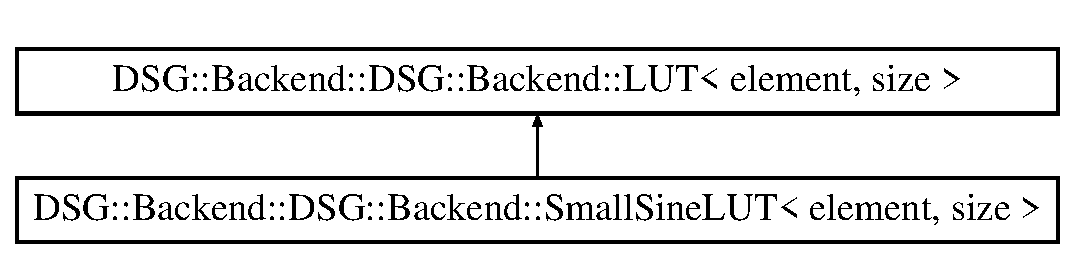
\includegraphics[height=2.000000cm]{classDSG_1_1Backend_1_1DSG_1_1Backend_1_1SmallSineLUT}
\end{center}
\end{figure}
\subsection*{Public Member Functions}
\begin{DoxyCompactItemize}
\item 
\hyperlink{classDSG_1_1Backend_1_1DSG_1_1Backend_1_1SmallSineLUT_a5da2128b03a551413c63f2dfe4c483d2}{Small\+Sine\+L\+U\+T} ()
\item 
virtual \hyperlink{classDSG_1_1Backend_1_1DSG_1_1Backend_1_1SmallSineLUT_aa33f15bd2f4a41916b2a143de41bc12d}{$\sim$\+Small\+Sine\+L\+U\+T} ()
\item 
virtual element \hyperlink{classDSG_1_1Backend_1_1DSG_1_1Backend_1_1SmallSineLUT_a2e15ffae0786ecc7a87d1202c5080850}{operator()} (double const \&x)
\item 
element const \& \hyperlink{classDSG_1_1Backend_1_1DSG_1_1Backend_1_1LUT_acd6db2fa4eba392de1cbb4795f351f8a}{operator\mbox{[}$\,$\mbox{]}} (unsigned long const \&index)
\item 
unsigned long const \& \hyperlink{classDSG_1_1Backend_1_1DSG_1_1Backend_1_1LUT_a65daa6f46f978a64da1c86089847602d}{Size} () const 
\end{DoxyCompactItemize}
\subsection*{Protected Member Functions}
\begin{DoxyCompactItemize}
\item 
void \hyperlink{classDSG_1_1Backend_1_1DSG_1_1Backend_1_1SmallSineLUT_aad31185d841e47300bf5b386e2c9e00f}{fill} ()
\item 
element const \& \hyperlink{classDSG_1_1Backend_1_1DSG_1_1Backend_1_1SmallSineLUT_acd4ee07b8be6fbd81b5ce70cd230ca4e}{lookup} (double index)
\end{DoxyCompactItemize}
\subsection*{Protected Attributes}
\begin{DoxyCompactItemize}
\item 
element \hyperlink{classDSG_1_1Backend_1_1DSG_1_1Backend_1_1LUT_a427da4b7eccdfe25e3c1889a8c2fdea6}{\+\_\+table} \mbox{[}size\mbox{]}
\item 
const unsigned long \hyperlink{classDSG_1_1Backend_1_1DSG_1_1Backend_1_1LUT_aa48956aa4debf08fdb517cb751d3e01d}{\+\_\+size}
\end{DoxyCompactItemize}


\subsection{Detailed Description}
\subsubsection*{template$<$typename element, unsigned long size$>$class D\+S\+G\+::\+Backend\+::\+D\+S\+G\+::\+Backend\+::\+Small\+Sine\+L\+U\+T$<$ element, size $>$}



Definition at line 48 of file Sin.\+h.



\subsection{Constructor \& Destructor Documentation}
\hypertarget{classDSG_1_1Backend_1_1DSG_1_1Backend_1_1SmallSineLUT_a5da2128b03a551413c63f2dfe4c483d2}{\index{D\+S\+G\+::\+Backend\+::\+D\+S\+G\+::\+Backend\+::\+Small\+Sine\+L\+U\+T@{D\+S\+G\+::\+Backend\+::\+D\+S\+G\+::\+Backend\+::\+Small\+Sine\+L\+U\+T}!Small\+Sine\+L\+U\+T@{Small\+Sine\+L\+U\+T}}
\index{Small\+Sine\+L\+U\+T@{Small\+Sine\+L\+U\+T}!D\+S\+G\+::\+Backend\+::\+D\+S\+G\+::\+Backend\+::\+Small\+Sine\+L\+U\+T@{D\+S\+G\+::\+Backend\+::\+D\+S\+G\+::\+Backend\+::\+Small\+Sine\+L\+U\+T}}
\subsubsection[{Small\+Sine\+L\+U\+T}]{\setlength{\rightskip}{0pt plus 5cm}template$<$typename element , unsigned long size$>$ {\bf D\+S\+G\+::\+Backend\+::\+D\+S\+G\+::\+Backend\+::\+Small\+Sine\+L\+U\+T}$<$ element, size $>$\+::{\bf Small\+Sine\+L\+U\+T} (
\begin{DoxyParamCaption}
{}
\end{DoxyParamCaption}
)\hspace{0.3cm}{\ttfamily [inline]}}}\label{classDSG_1_1Backend_1_1DSG_1_1Backend_1_1SmallSineLUT_a5da2128b03a551413c63f2dfe4c483d2}


Definition at line 50 of file Sin.\+h.

\hypertarget{classDSG_1_1Backend_1_1DSG_1_1Backend_1_1SmallSineLUT_aa33f15bd2f4a41916b2a143de41bc12d}{\index{D\+S\+G\+::\+Backend\+::\+D\+S\+G\+::\+Backend\+::\+Small\+Sine\+L\+U\+T@{D\+S\+G\+::\+Backend\+::\+D\+S\+G\+::\+Backend\+::\+Small\+Sine\+L\+U\+T}!````~Small\+Sine\+L\+U\+T@{$\sim$\+Small\+Sine\+L\+U\+T}}
\index{````~Small\+Sine\+L\+U\+T@{$\sim$\+Small\+Sine\+L\+U\+T}!D\+S\+G\+::\+Backend\+::\+D\+S\+G\+::\+Backend\+::\+Small\+Sine\+L\+U\+T@{D\+S\+G\+::\+Backend\+::\+D\+S\+G\+::\+Backend\+::\+Small\+Sine\+L\+U\+T}}
\subsubsection[{$\sim$\+Small\+Sine\+L\+U\+T}]{\setlength{\rightskip}{0pt plus 5cm}template$<$typename element , unsigned long size$>$ virtual {\bf D\+S\+G\+::\+Backend\+::\+D\+S\+G\+::\+Backend\+::\+Small\+Sine\+L\+U\+T}$<$ element, size $>$\+::$\sim${\bf Small\+Sine\+L\+U\+T} (
\begin{DoxyParamCaption}
{}
\end{DoxyParamCaption}
)\hspace{0.3cm}{\ttfamily [inline]}, {\ttfamily [virtual]}}}\label{classDSG_1_1Backend_1_1DSG_1_1Backend_1_1SmallSineLUT_aa33f15bd2f4a41916b2a143de41bc12d}


Definition at line 51 of file Sin.\+h.



\subsection{Member Function Documentation}
\hypertarget{classDSG_1_1Backend_1_1DSG_1_1Backend_1_1SmallSineLUT_aad31185d841e47300bf5b386e2c9e00f}{\index{D\+S\+G\+::\+Backend\+::\+D\+S\+G\+::\+Backend\+::\+Small\+Sine\+L\+U\+T@{D\+S\+G\+::\+Backend\+::\+D\+S\+G\+::\+Backend\+::\+Small\+Sine\+L\+U\+T}!fill@{fill}}
\index{fill@{fill}!D\+S\+G\+::\+Backend\+::\+D\+S\+G\+::\+Backend\+::\+Small\+Sine\+L\+U\+T@{D\+S\+G\+::\+Backend\+::\+D\+S\+G\+::\+Backend\+::\+Small\+Sine\+L\+U\+T}}
\subsubsection[{fill}]{\setlength{\rightskip}{0pt plus 5cm}template$<$typename element , unsigned long size$>$ void {\bf D\+S\+G\+::\+Backend\+::\+D\+S\+G\+::\+Backend\+::\+Small\+Sine\+L\+U\+T}$<$ element, size $>$\+::fill (
\begin{DoxyParamCaption}
{}
\end{DoxyParamCaption}
)\hspace{0.3cm}{\ttfamily [inline]}, {\ttfamily [protected]}}}\label{classDSG_1_1Backend_1_1DSG_1_1Backend_1_1SmallSineLUT_aad31185d841e47300bf5b386e2c9e00f}


Definition at line 74 of file Sin.\+h.

\hypertarget{classDSG_1_1Backend_1_1DSG_1_1Backend_1_1SmallSineLUT_acd4ee07b8be6fbd81b5ce70cd230ca4e}{\index{D\+S\+G\+::\+Backend\+::\+D\+S\+G\+::\+Backend\+::\+Small\+Sine\+L\+U\+T@{D\+S\+G\+::\+Backend\+::\+D\+S\+G\+::\+Backend\+::\+Small\+Sine\+L\+U\+T}!lookup@{lookup}}
\index{lookup@{lookup}!D\+S\+G\+::\+Backend\+::\+D\+S\+G\+::\+Backend\+::\+Small\+Sine\+L\+U\+T@{D\+S\+G\+::\+Backend\+::\+D\+S\+G\+::\+Backend\+::\+Small\+Sine\+L\+U\+T}}
\subsubsection[{lookup}]{\setlength{\rightskip}{0pt plus 5cm}template$<$typename element , unsigned long size$>$ element const\& {\bf D\+S\+G\+::\+Backend\+::\+D\+S\+G\+::\+Backend\+::\+Small\+Sine\+L\+U\+T}$<$ element, size $>$\+::lookup (
\begin{DoxyParamCaption}
\item[{double}]{index}
\end{DoxyParamCaption}
)\hspace{0.3cm}{\ttfamily [inline]}, {\ttfamily [protected]}}}\label{classDSG_1_1Backend_1_1DSG_1_1Backend_1_1SmallSineLUT_acd4ee07b8be6fbd81b5ce70cd230ca4e}


Definition at line 82 of file Sin.\+h.

\hypertarget{classDSG_1_1Backend_1_1DSG_1_1Backend_1_1SmallSineLUT_a2e15ffae0786ecc7a87d1202c5080850}{\index{D\+S\+G\+::\+Backend\+::\+D\+S\+G\+::\+Backend\+::\+Small\+Sine\+L\+U\+T@{D\+S\+G\+::\+Backend\+::\+D\+S\+G\+::\+Backend\+::\+Small\+Sine\+L\+U\+T}!operator()@{operator()}}
\index{operator()@{operator()}!D\+S\+G\+::\+Backend\+::\+D\+S\+G\+::\+Backend\+::\+Small\+Sine\+L\+U\+T@{D\+S\+G\+::\+Backend\+::\+D\+S\+G\+::\+Backend\+::\+Small\+Sine\+L\+U\+T}}
\subsubsection[{operator()}]{\setlength{\rightskip}{0pt plus 5cm}template$<$typename element , unsigned long size$>$ virtual element {\bf D\+S\+G\+::\+Backend\+::\+D\+S\+G\+::\+Backend\+::\+Small\+Sine\+L\+U\+T}$<$ element, size $>$\+::operator() (
\begin{DoxyParamCaption}
\item[{double const \&}]{x}
\end{DoxyParamCaption}
)\hspace{0.3cm}{\ttfamily [inline]}, {\ttfamily [virtual]}}}\label{classDSG_1_1Backend_1_1DSG_1_1Backend_1_1SmallSineLUT_a2e15ffae0786ecc7a87d1202c5080850}


Reimplemented from \hyperlink{classDSG_1_1Backend_1_1DSG_1_1Backend_1_1LUT_a4cdb48ce3c472160931968739623f8ac}{D\+S\+G\+::\+Backend\+::\+D\+S\+G\+::\+Backend\+::\+L\+U\+T$<$ element, size $>$}.



Definition at line 52 of file Sin.\+h.

\hypertarget{classDSG_1_1Backend_1_1DSG_1_1Backend_1_1LUT_acd6db2fa4eba392de1cbb4795f351f8a}{\index{D\+S\+G\+::\+Backend\+::\+D\+S\+G\+::\+Backend\+::\+Small\+Sine\+L\+U\+T@{D\+S\+G\+::\+Backend\+::\+D\+S\+G\+::\+Backend\+::\+Small\+Sine\+L\+U\+T}!operator\mbox{[}$\,$\mbox{]}@{operator[]}}
\index{operator\mbox{[}$\,$\mbox{]}@{operator[]}!D\+S\+G\+::\+Backend\+::\+D\+S\+G\+::\+Backend\+::\+Small\+Sine\+L\+U\+T@{D\+S\+G\+::\+Backend\+::\+D\+S\+G\+::\+Backend\+::\+Small\+Sine\+L\+U\+T}}
\subsubsection[{operator[]}]{\setlength{\rightskip}{0pt plus 5cm}template$<$typename element, unsigned long size$>$ element const\& {\bf D\+S\+G\+::\+Backend\+::\+D\+S\+G\+::\+Backend\+::\+L\+U\+T}$<$ element, size $>$\+::operator\mbox{[}$\,$\mbox{]} (
\begin{DoxyParamCaption}
\item[{unsigned long const \&}]{index}
\end{DoxyParamCaption}
)\hspace{0.3cm}{\ttfamily [inline]}, {\ttfamily [inherited]}}}\label{classDSG_1_1Backend_1_1DSG_1_1Backend_1_1LUT_acd6db2fa4eba392de1cbb4795f351f8a}


Definition at line 24 of file Sin.\+h.


\begin{DoxyCode}
33                                         \{
\end{DoxyCode}
\hypertarget{classDSG_1_1Backend_1_1DSG_1_1Backend_1_1LUT_a65daa6f46f978a64da1c86089847602d}{\index{D\+S\+G\+::\+Backend\+::\+D\+S\+G\+::\+Backend\+::\+Small\+Sine\+L\+U\+T@{D\+S\+G\+::\+Backend\+::\+D\+S\+G\+::\+Backend\+::\+Small\+Sine\+L\+U\+T}!Size@{Size}}
\index{Size@{Size}!D\+S\+G\+::\+Backend\+::\+D\+S\+G\+::\+Backend\+::\+Small\+Sine\+L\+U\+T@{D\+S\+G\+::\+Backend\+::\+D\+S\+G\+::\+Backend\+::\+Small\+Sine\+L\+U\+T}}
\subsubsection[{Size}]{\setlength{\rightskip}{0pt plus 5cm}template$<$typename element, unsigned long size$>$ unsigned long const\& {\bf D\+S\+G\+::\+Backend\+::\+D\+S\+G\+::\+Backend\+::\+L\+U\+T}$<$ element, size $>$\+::Size (
\begin{DoxyParamCaption}
{}
\end{DoxyParamCaption}
) const\hspace{0.3cm}{\ttfamily [inline]}, {\ttfamily [inherited]}}}\label{classDSG_1_1Backend_1_1DSG_1_1Backend_1_1LUT_a65daa6f46f978a64da1c86089847602d}


Definition at line 33 of file Sin.\+h.


\begin{DoxyCode}
33                                         \{
34         \textcolor{comment}{//phs 0-1}
35 \textcolor{preprocessor}{#if sin\_impl == sin\_native}
\end{DoxyCode}


\subsection{Member Data Documentation}
\hypertarget{classDSG_1_1Backend_1_1DSG_1_1Backend_1_1LUT_aa48956aa4debf08fdb517cb751d3e01d}{\index{D\+S\+G\+::\+Backend\+::\+D\+S\+G\+::\+Backend\+::\+Small\+Sine\+L\+U\+T@{D\+S\+G\+::\+Backend\+::\+D\+S\+G\+::\+Backend\+::\+Small\+Sine\+L\+U\+T}!\+\_\+size@{\+\_\+size}}
\index{\+\_\+size@{\+\_\+size}!D\+S\+G\+::\+Backend\+::\+D\+S\+G\+::\+Backend\+::\+Small\+Sine\+L\+U\+T@{D\+S\+G\+::\+Backend\+::\+D\+S\+G\+::\+Backend\+::\+Small\+Sine\+L\+U\+T}}
\subsubsection[{\+\_\+size}]{\setlength{\rightskip}{0pt plus 5cm}template$<$typename element, unsigned long size$>$ const unsigned long {\bf D\+S\+G\+::\+Backend\+::\+D\+S\+G\+::\+Backend\+::\+L\+U\+T}$<$ element, size $>$\+::\+\_\+size\hspace{0.3cm}{\ttfamily [protected]}, {\ttfamily [inherited]}}}\label{classDSG_1_1Backend_1_1DSG_1_1Backend_1_1LUT_aa48956aa4debf08fdb517cb751d3e01d}


Definition at line 38 of file Sin.\+h.

\hypertarget{classDSG_1_1Backend_1_1DSG_1_1Backend_1_1LUT_a427da4b7eccdfe25e3c1889a8c2fdea6}{\index{D\+S\+G\+::\+Backend\+::\+D\+S\+G\+::\+Backend\+::\+Small\+Sine\+L\+U\+T@{D\+S\+G\+::\+Backend\+::\+D\+S\+G\+::\+Backend\+::\+Small\+Sine\+L\+U\+T}!\+\_\+table@{\+\_\+table}}
\index{\+\_\+table@{\+\_\+table}!D\+S\+G\+::\+Backend\+::\+D\+S\+G\+::\+Backend\+::\+Small\+Sine\+L\+U\+T@{D\+S\+G\+::\+Backend\+::\+D\+S\+G\+::\+Backend\+::\+Small\+Sine\+L\+U\+T}}
\subsubsection[{\+\_\+table}]{\setlength{\rightskip}{0pt plus 5cm}template$<$typename element, unsigned long size$>$ element {\bf D\+S\+G\+::\+Backend\+::\+D\+S\+G\+::\+Backend\+::\+L\+U\+T}$<$ element, size $>$\+::\+\_\+table\mbox{[}size\mbox{]}\hspace{0.3cm}{\ttfamily [protected]}, {\ttfamily [inherited]}}}\label{classDSG_1_1Backend_1_1DSG_1_1Backend_1_1LUT_a427da4b7eccdfe25e3c1889a8c2fdea6}


Definition at line 37 of file Sin.\+h.



The documentation for this class was generated from the following file\+:\begin{DoxyCompactItemize}
\item 
/\+Users/alexanderzywicki/\+Documents/\+School\+\_\+\+Stuff/\+Fall\+\_\+2014/\+Digital\+\_\+\+Signal\+\_\+\+Generation\+\_\+and\+\_\+\+Analysis/src/include/\hyperlink{Sin_8h}{Sin.\+h}\end{DoxyCompactItemize}

\hypertarget{classDSG_1_1Backend_1_1DSG_1_1Backend_1_1SmallSineLUT_3_01int32__t_00_01size_01_4}{\section{D\+S\+G\+:\+:Backend\+:\+:D\+S\+G\+:\+:Backend\+:\+:Small\+Sine\+L\+U\+T$<$ int32\+\_\+t, size $>$ Class Template Reference}
\label{classDSG_1_1Backend_1_1DSG_1_1Backend_1_1SmallSineLUT_3_01int32__t_00_01size_01_4}\index{D\+S\+G\+::\+Backend\+::\+D\+S\+G\+::\+Backend\+::\+Small\+Sine\+L\+U\+T$<$ int32\+\_\+t, size $>$@{D\+S\+G\+::\+Backend\+::\+D\+S\+G\+::\+Backend\+::\+Small\+Sine\+L\+U\+T$<$ int32\+\_\+t, size $>$}}
}


{\ttfamily \#include $<$Sin.\+h$>$}

Inheritance diagram for D\+S\+G\+:\+:Backend\+:\+:D\+S\+G\+:\+:Backend\+:\+:Small\+Sine\+L\+U\+T$<$ int32\+\_\+t, size $>$\+:\begin{figure}[H]
\begin{center}
\leavevmode
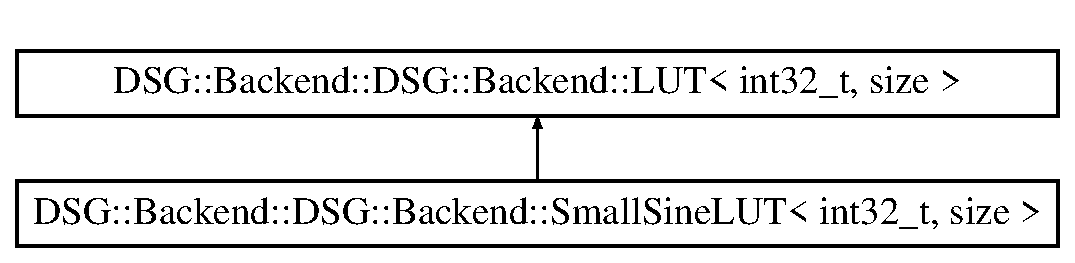
\includegraphics[height=2.000000cm]{classDSG_1_1Backend_1_1DSG_1_1Backend_1_1SmallSineLUT_3_01int32__t_00_01size_01_4}
\end{center}
\end{figure}
\subsection*{Public Member Functions}
\begin{DoxyCompactItemize}
\item 
\hyperlink{classDSG_1_1Backend_1_1DSG_1_1Backend_1_1SmallSineLUT_3_01int32__t_00_01size_01_4_abef6922af5561ae0edfb55b3307dd918}{Small\+Sine\+L\+U\+T} ()
\item 
virtual \hyperlink{classDSG_1_1Backend_1_1DSG_1_1Backend_1_1SmallSineLUT_3_01int32__t_00_01size_01_4_af117c305819a522714c29bd00e1079d1}{$\sim$\+Small\+Sine\+L\+U\+T} ()
\item 
virtual int32\+\_\+t \hyperlink{classDSG_1_1Backend_1_1DSG_1_1Backend_1_1SmallSineLUT_3_01int32__t_00_01size_01_4_a6093cb33233f44ac97d15998dc0ba005}{operator()} (double const \&x)
\item 
int32\+\_\+tconst \& \hyperlink{classDSG_1_1Backend_1_1DSG_1_1Backend_1_1LUT_acd6db2fa4eba392de1cbb4795f351f8a}{operator\mbox{[}$\,$\mbox{]}} (unsigned long const \&index)
\item 
unsigned long const \& \hyperlink{classDSG_1_1Backend_1_1DSG_1_1Backend_1_1LUT_a65daa6f46f978a64da1c86089847602d}{Size} () const
\end{DoxyCompactItemize}
\subsection*{Protected Member Functions}
\begin{DoxyCompactItemize}
\item 
void \hyperlink{classDSG_1_1Backend_1_1DSG_1_1Backend_1_1SmallSineLUT_3_01int32__t_00_01size_01_4_a05c97d82f124088ad802ce5db5b6290b}{fill} ()
\item 
int32\+\_\+t const \& \hyperlink{classDSG_1_1Backend_1_1DSG_1_1Backend_1_1SmallSineLUT_3_01int32__t_00_01size_01_4_adc63dbfd6169d226255d6bc5c61d4c00}{lookup} (double \&\&index)
\end{DoxyCompactItemize}
\subsection*{Protected Attributes}
\begin{DoxyCompactItemize}
\item 
int32\+\_\+t \hyperlink{classDSG_1_1Backend_1_1DSG_1_1Backend_1_1LUT_a427da4b7eccdfe25e3c1889a8c2fdea6}{\+\_\+table} \mbox{[}size\mbox{]}
\item 
const unsigned long \hyperlink{classDSG_1_1Backend_1_1DSG_1_1Backend_1_1LUT_aa48956aa4debf08fdb517cb751d3e01d}{\+\_\+size}
\end{DoxyCompactItemize}


\subsection{Detailed Description}
\subsubsection*{template$<$unsigned long size$>$class D\+S\+G\+::\+Backend\+::\+D\+S\+G\+::\+Backend\+::\+Small\+Sine\+L\+U\+T$<$ int32\+\_\+t, size $>$}



Definition at line 91 of file Sin.\+h.



\subsection{Constructor \& Destructor Documentation}
\hypertarget{classDSG_1_1Backend_1_1DSG_1_1Backend_1_1SmallSineLUT_3_01int32__t_00_01size_01_4_abef6922af5561ae0edfb55b3307dd918}{\index{D\+S\+G\+::\+Backend\+::\+D\+S\+G\+::\+Backend\+::\+Small\+Sine\+L\+U\+T$<$ int32\+\_\+t, size $>$@{D\+S\+G\+::\+Backend\+::\+D\+S\+G\+::\+Backend\+::\+Small\+Sine\+L\+U\+T$<$ int32\+\_\+t, size $>$}!Small\+Sine\+L\+U\+T@{Small\+Sine\+L\+U\+T}}
\index{Small\+Sine\+L\+U\+T@{Small\+Sine\+L\+U\+T}!D\+S\+G\+::\+Backend\+::\+D\+S\+G\+::\+Backend\+::\+Small\+Sine\+L\+U\+T$<$ int32\+\_\+t, size $>$@{D\+S\+G\+::\+Backend\+::\+D\+S\+G\+::\+Backend\+::\+Small\+Sine\+L\+U\+T$<$ int32\+\_\+t, size $>$}}
\subsubsection[{Small\+Sine\+L\+U\+T}]{\setlength{\rightskip}{0pt plus 5cm}template$<$unsigned long size$>$ {\bf D\+S\+G\+::\+Backend\+::\+D\+S\+G\+::\+Backend\+::\+Small\+Sine\+L\+U\+T}$<$ int32\+\_\+t, size $>$\+::{\bf Small\+Sine\+L\+U\+T} (
\begin{DoxyParamCaption}
{}
\end{DoxyParamCaption}
)\hspace{0.3cm}{\ttfamily [inline]}}}\label{classDSG_1_1Backend_1_1DSG_1_1Backend_1_1SmallSineLUT_3_01int32__t_00_01size_01_4_abef6922af5561ae0edfb55b3307dd918}


Definition at line 93 of file Sin.\+h.

\hypertarget{classDSG_1_1Backend_1_1DSG_1_1Backend_1_1SmallSineLUT_3_01int32__t_00_01size_01_4_af117c305819a522714c29bd00e1079d1}{\index{D\+S\+G\+::\+Backend\+::\+D\+S\+G\+::\+Backend\+::\+Small\+Sine\+L\+U\+T$<$ int32\+\_\+t, size $>$@{D\+S\+G\+::\+Backend\+::\+D\+S\+G\+::\+Backend\+::\+Small\+Sine\+L\+U\+T$<$ int32\+\_\+t, size $>$}!````~Small\+Sine\+L\+U\+T@{$\sim$\+Small\+Sine\+L\+U\+T}}
\index{````~Small\+Sine\+L\+U\+T@{$\sim$\+Small\+Sine\+L\+U\+T}!D\+S\+G\+::\+Backend\+::\+D\+S\+G\+::\+Backend\+::\+Small\+Sine\+L\+U\+T$<$ int32\+\_\+t, size $>$@{D\+S\+G\+::\+Backend\+::\+D\+S\+G\+::\+Backend\+::\+Small\+Sine\+L\+U\+T$<$ int32\+\_\+t, size $>$}}
\subsubsection[{$\sim$\+Small\+Sine\+L\+U\+T}]{\setlength{\rightskip}{0pt plus 5cm}template$<$unsigned long size$>$ virtual {\bf D\+S\+G\+::\+Backend\+::\+D\+S\+G\+::\+Backend\+::\+Small\+Sine\+L\+U\+T}$<$ int32\+\_\+t, size $>$\+::$\sim${\bf Small\+Sine\+L\+U\+T} (
\begin{DoxyParamCaption}
{}
\end{DoxyParamCaption}
)\hspace{0.3cm}{\ttfamily [inline]}, {\ttfamily [virtual]}}}\label{classDSG_1_1Backend_1_1DSG_1_1Backend_1_1SmallSineLUT_3_01int32__t_00_01size_01_4_af117c305819a522714c29bd00e1079d1}


Definition at line 94 of file Sin.\+h.



\subsection{Member Function Documentation}
\hypertarget{classDSG_1_1Backend_1_1DSG_1_1Backend_1_1SmallSineLUT_3_01int32__t_00_01size_01_4_a05c97d82f124088ad802ce5db5b6290b}{\index{D\+S\+G\+::\+Backend\+::\+D\+S\+G\+::\+Backend\+::\+Small\+Sine\+L\+U\+T$<$ int32\+\_\+t, size $>$@{D\+S\+G\+::\+Backend\+::\+D\+S\+G\+::\+Backend\+::\+Small\+Sine\+L\+U\+T$<$ int32\+\_\+t, size $>$}!fill@{fill}}
\index{fill@{fill}!D\+S\+G\+::\+Backend\+::\+D\+S\+G\+::\+Backend\+::\+Small\+Sine\+L\+U\+T$<$ int32\+\_\+t, size $>$@{D\+S\+G\+::\+Backend\+::\+D\+S\+G\+::\+Backend\+::\+Small\+Sine\+L\+U\+T$<$ int32\+\_\+t, size $>$}}
\subsubsection[{fill}]{\setlength{\rightskip}{0pt plus 5cm}template$<$unsigned long size$>$ void {\bf D\+S\+G\+::\+Backend\+::\+D\+S\+G\+::\+Backend\+::\+Small\+Sine\+L\+U\+T}$<$ int32\+\_\+t, size $>$\+::fill (
\begin{DoxyParamCaption}
{}
\end{DoxyParamCaption}
)\hspace{0.3cm}{\ttfamily [inline]}, {\ttfamily [protected]}}}\label{classDSG_1_1Backend_1_1DSG_1_1Backend_1_1SmallSineLUT_3_01int32__t_00_01size_01_4_a05c97d82f124088ad802ce5db5b6290b}


Definition at line 121 of file Sin.\+h.

\hypertarget{classDSG_1_1Backend_1_1DSG_1_1Backend_1_1SmallSineLUT_3_01int32__t_00_01size_01_4_adc63dbfd6169d226255d6bc5c61d4c00}{\index{D\+S\+G\+::\+Backend\+::\+D\+S\+G\+::\+Backend\+::\+Small\+Sine\+L\+U\+T$<$ int32\+\_\+t, size $>$@{D\+S\+G\+::\+Backend\+::\+D\+S\+G\+::\+Backend\+::\+Small\+Sine\+L\+U\+T$<$ int32\+\_\+t, size $>$}!lookup@{lookup}}
\index{lookup@{lookup}!D\+S\+G\+::\+Backend\+::\+D\+S\+G\+::\+Backend\+::\+Small\+Sine\+L\+U\+T$<$ int32\+\_\+t, size $>$@{D\+S\+G\+::\+Backend\+::\+D\+S\+G\+::\+Backend\+::\+Small\+Sine\+L\+U\+T$<$ int32\+\_\+t, size $>$}}
\subsubsection[{lookup}]{\setlength{\rightskip}{0pt plus 5cm}template$<$unsigned long size$>$ int32\+\_\+t const\& {\bf D\+S\+G\+::\+Backend\+::\+D\+S\+G\+::\+Backend\+::\+Small\+Sine\+L\+U\+T}$<$ int32\+\_\+t, size $>$\+::lookup (
\begin{DoxyParamCaption}
\item[{double \&\&}]{index}
\end{DoxyParamCaption}
)\hspace{0.3cm}{\ttfamily [inline]}, {\ttfamily [protected]}}}\label{classDSG_1_1Backend_1_1DSG_1_1Backend_1_1SmallSineLUT_3_01int32__t_00_01size_01_4_adc63dbfd6169d226255d6bc5c61d4c00}


Definition at line 130 of file Sin.\+h.

\hypertarget{classDSG_1_1Backend_1_1DSG_1_1Backend_1_1SmallSineLUT_3_01int32__t_00_01size_01_4_a6093cb33233f44ac97d15998dc0ba005}{\index{D\+S\+G\+::\+Backend\+::\+D\+S\+G\+::\+Backend\+::\+Small\+Sine\+L\+U\+T$<$ int32\+\_\+t, size $>$@{D\+S\+G\+::\+Backend\+::\+D\+S\+G\+::\+Backend\+::\+Small\+Sine\+L\+U\+T$<$ int32\+\_\+t, size $>$}!operator()@{operator()}}
\index{operator()@{operator()}!D\+S\+G\+::\+Backend\+::\+D\+S\+G\+::\+Backend\+::\+Small\+Sine\+L\+U\+T$<$ int32\+\_\+t, size $>$@{D\+S\+G\+::\+Backend\+::\+D\+S\+G\+::\+Backend\+::\+Small\+Sine\+L\+U\+T$<$ int32\+\_\+t, size $>$}}
\subsubsection[{operator()}]{\setlength{\rightskip}{0pt plus 5cm}template$<$unsigned long size$>$ virtual int32\+\_\+t {\bf D\+S\+G\+::\+Backend\+::\+D\+S\+G\+::\+Backend\+::\+Small\+Sine\+L\+U\+T}$<$ int32\+\_\+t, size $>$\+::operator() (
\begin{DoxyParamCaption}
\item[{double const \&}]{x}
\end{DoxyParamCaption}
)\hspace{0.3cm}{\ttfamily [inline]}, {\ttfamily [virtual]}}}\label{classDSG_1_1Backend_1_1DSG_1_1Backend_1_1SmallSineLUT_3_01int32__t_00_01size_01_4_a6093cb33233f44ac97d15998dc0ba005}


Reimplemented from \hyperlink{classDSG_1_1Backend_1_1DSG_1_1Backend_1_1LUT_a4cdb48ce3c472160931968739623f8ac}{D\+S\+G\+::\+Backend\+::\+D\+S\+G\+::\+Backend\+::\+L\+U\+T$<$ int32\+\_\+t, size $>$}.



Definition at line 95 of file Sin.\+h.

\hypertarget{classDSG_1_1Backend_1_1DSG_1_1Backend_1_1LUT_acd6db2fa4eba392de1cbb4795f351f8a}{\index{D\+S\+G\+::\+Backend\+::\+D\+S\+G\+::\+Backend\+::\+Small\+Sine\+L\+U\+T$<$ int32\+\_\+t, size $>$@{D\+S\+G\+::\+Backend\+::\+D\+S\+G\+::\+Backend\+::\+Small\+Sine\+L\+U\+T$<$ int32\+\_\+t, size $>$}!operator\mbox{[}$\,$\mbox{]}@{operator[]}}
\index{operator\mbox{[}$\,$\mbox{]}@{operator[]}!D\+S\+G\+::\+Backend\+::\+D\+S\+G\+::\+Backend\+::\+Small\+Sine\+L\+U\+T$<$ int32\+\_\+t, size $>$@{D\+S\+G\+::\+Backend\+::\+D\+S\+G\+::\+Backend\+::\+Small\+Sine\+L\+U\+T$<$ int32\+\_\+t, size $>$}}
\subsubsection[{operator[]}]{\setlength{\rightskip}{0pt plus 5cm}int32\+\_\+t  const\& {\bf D\+S\+G\+::\+Backend\+::\+D\+S\+G\+::\+Backend\+::\+L\+U\+T}$<$ int32\+\_\+t , size $>$\+::operator\mbox{[}$\,$\mbox{]} (
\begin{DoxyParamCaption}
\item[{unsigned long const \&}]{index}
\end{DoxyParamCaption}
)\hspace{0.3cm}{\ttfamily [inline]}, {\ttfamily [inherited]}}}\label{classDSG_1_1Backend_1_1DSG_1_1Backend_1_1LUT_acd6db2fa4eba392de1cbb4795f351f8a}


Definition at line 24 of file Sin.\+h.


\begin{DoxyCode}
33                                         \{
\end{DoxyCode}
\hypertarget{classDSG_1_1Backend_1_1DSG_1_1Backend_1_1LUT_a65daa6f46f978a64da1c86089847602d}{\index{D\+S\+G\+::\+Backend\+::\+D\+S\+G\+::\+Backend\+::\+Small\+Sine\+L\+U\+T$<$ int32\+\_\+t, size $>$@{D\+S\+G\+::\+Backend\+::\+D\+S\+G\+::\+Backend\+::\+Small\+Sine\+L\+U\+T$<$ int32\+\_\+t, size $>$}!Size@{Size}}
\index{Size@{Size}!D\+S\+G\+::\+Backend\+::\+D\+S\+G\+::\+Backend\+::\+Small\+Sine\+L\+U\+T$<$ int32\+\_\+t, size $>$@{D\+S\+G\+::\+Backend\+::\+D\+S\+G\+::\+Backend\+::\+Small\+Sine\+L\+U\+T$<$ int32\+\_\+t, size $>$}}
\subsubsection[{Size}]{\setlength{\rightskip}{0pt plus 5cm}unsigned long const\& {\bf D\+S\+G\+::\+Backend\+::\+D\+S\+G\+::\+Backend\+::\+L\+U\+T}$<$ int32\+\_\+t , size $>$\+::Size (
\begin{DoxyParamCaption}
{}
\end{DoxyParamCaption}
) const\hspace{0.3cm}{\ttfamily [inline]}, {\ttfamily [inherited]}}}\label{classDSG_1_1Backend_1_1DSG_1_1Backend_1_1LUT_a65daa6f46f978a64da1c86089847602d}


Definition at line 33 of file Sin.\+h.


\begin{DoxyCode}
33                                         \{
34         \textcolor{comment}{//phs 0-1}
35 \textcolor{preprocessor}{#if sin\_impl == sin\_native}
\end{DoxyCode}


\subsection{Member Data Documentation}
\hypertarget{classDSG_1_1Backend_1_1DSG_1_1Backend_1_1LUT_aa48956aa4debf08fdb517cb751d3e01d}{\index{D\+S\+G\+::\+Backend\+::\+D\+S\+G\+::\+Backend\+::\+Small\+Sine\+L\+U\+T$<$ int32\+\_\+t, size $>$@{D\+S\+G\+::\+Backend\+::\+D\+S\+G\+::\+Backend\+::\+Small\+Sine\+L\+U\+T$<$ int32\+\_\+t, size $>$}!\+\_\+size@{\+\_\+size}}
\index{\+\_\+size@{\+\_\+size}!D\+S\+G\+::\+Backend\+::\+D\+S\+G\+::\+Backend\+::\+Small\+Sine\+L\+U\+T$<$ int32\+\_\+t, size $>$@{D\+S\+G\+::\+Backend\+::\+D\+S\+G\+::\+Backend\+::\+Small\+Sine\+L\+U\+T$<$ int32\+\_\+t, size $>$}}
\subsubsection[{\+\_\+size}]{\setlength{\rightskip}{0pt plus 5cm}const unsigned long {\bf D\+S\+G\+::\+Backend\+::\+D\+S\+G\+::\+Backend\+::\+L\+U\+T}$<$ int32\+\_\+t , size $>$\+::\+\_\+size\hspace{0.3cm}{\ttfamily [protected]}, {\ttfamily [inherited]}}}\label{classDSG_1_1Backend_1_1DSG_1_1Backend_1_1LUT_aa48956aa4debf08fdb517cb751d3e01d}


Definition at line 38 of file Sin.\+h.

\hypertarget{classDSG_1_1Backend_1_1DSG_1_1Backend_1_1LUT_a427da4b7eccdfe25e3c1889a8c2fdea6}{\index{D\+S\+G\+::\+Backend\+::\+D\+S\+G\+::\+Backend\+::\+Small\+Sine\+L\+U\+T$<$ int32\+\_\+t, size $>$@{D\+S\+G\+::\+Backend\+::\+D\+S\+G\+::\+Backend\+::\+Small\+Sine\+L\+U\+T$<$ int32\+\_\+t, size $>$}!\+\_\+table@{\+\_\+table}}
\index{\+\_\+table@{\+\_\+table}!D\+S\+G\+::\+Backend\+::\+D\+S\+G\+::\+Backend\+::\+Small\+Sine\+L\+U\+T$<$ int32\+\_\+t, size $>$@{D\+S\+G\+::\+Backend\+::\+D\+S\+G\+::\+Backend\+::\+Small\+Sine\+L\+U\+T$<$ int32\+\_\+t, size $>$}}
\subsubsection[{\+\_\+table}]{\setlength{\rightskip}{0pt plus 5cm}int32\+\_\+t  {\bf D\+S\+G\+::\+Backend\+::\+D\+S\+G\+::\+Backend\+::\+L\+U\+T}$<$ int32\+\_\+t , size $>$\+::\+\_\+table\mbox{[}size\mbox{]}\hspace{0.3cm}{\ttfamily [protected]}, {\ttfamily [inherited]}}}\label{classDSG_1_1Backend_1_1DSG_1_1Backend_1_1LUT_a427da4b7eccdfe25e3c1889a8c2fdea6}


Definition at line 37 of file Sin.\+h.



The documentation for this class was generated from the following file\+:\begin{DoxyCompactItemize}
\item 
/\+Users/alexanderzywicki/\+Documents/\+School\+\_\+\+Stuff/\+Fall\+\_\+2014/\+Digital\+\_\+\+Signal\+\_\+\+Generation\+\_\+and\+\_\+\+Analysis/src/include/\hyperlink{Sin_8h}{Sin.\+h}\end{DoxyCompactItemize}

\hypertarget{classDSG_1_1Backend_1_1SmallSineLUT_3_01int32__t_00_01size_01_4}{\section{D\+S\+G\+:\+:Backend\+:\+:Small\+Sine\+L\+U\+T$<$ int32\+\_\+t, size $>$ Class Template Reference}
\label{classDSG_1_1Backend_1_1SmallSineLUT_3_01int32__t_00_01size_01_4}\index{D\+S\+G\+::\+Backend\+::\+Small\+Sine\+L\+U\+T$<$ int32\+\_\+t, size $>$@{D\+S\+G\+::\+Backend\+::\+Small\+Sine\+L\+U\+T$<$ int32\+\_\+t, size $>$}}
}


{\ttfamily \#include $<$Sine\+L\+U\+T.\+h$>$}

Inheritance diagram for D\+S\+G\+:\+:Backend\+:\+:Small\+Sine\+L\+U\+T$<$ int32\+\_\+t, size $>$\+:\begin{figure}[H]
\begin{center}
\leavevmode
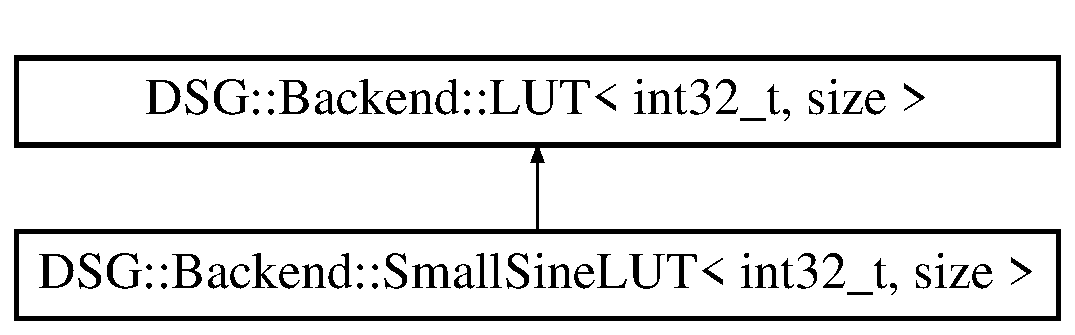
\includegraphics[height=2.000000cm]{classDSG_1_1Backend_1_1SmallSineLUT_3_01int32__t_00_01size_01_4}
\end{center}
\end{figure}
\subsection*{Public Member Functions}
\begin{DoxyCompactItemize}
\item 
\hyperlink{classDSG_1_1Backend_1_1SmallSineLUT_3_01int32__t_00_01size_01_4_ad6c60ff274c31fa8aac6353b9089a8e8}{Small\+Sine\+L\+U\+T} ()
\item 
virtual \hyperlink{classDSG_1_1Backend_1_1SmallSineLUT_3_01int32__t_00_01size_01_4_a1c8fd85f2ce8d0283997096159442678}{$\sim$\+Small\+Sine\+L\+U\+T} ()
\item 
virtual int32\+\_\+t \hyperlink{classDSG_1_1Backend_1_1SmallSineLUT_3_01int32__t_00_01size_01_4_af8b347ef429ec5b6edbe7b752a003d2e}{operator()} (double const \&x)
\item 
int32\+\_\+tconst \& \hyperlink{classDSG_1_1Backend_1_1LUT_a50d8304c33760ed566039ebf5657807c}{operator\mbox{[}$\,$\mbox{]}} (unsigned long const \&index)
\item 
unsigned long const \& \hyperlink{classDSG_1_1Backend_1_1LUT_a988c07b5002e0aee6e490244b80c8830}{Size} () const
\end{DoxyCompactItemize}
\subsection*{Protected Member Functions}
\begin{DoxyCompactItemize}
\item 
void \hyperlink{classDSG_1_1Backend_1_1SmallSineLUT_3_01int32__t_00_01size_01_4_a88c1a17c38d0f8767bfdc899a22f7eba}{fill} ()
\item 
int32\+\_\+t const \& \hyperlink{classDSG_1_1Backend_1_1SmallSineLUT_3_01int32__t_00_01size_01_4_a9635d6cb5dd66d17c61ce09b3e437217}{lookup} (double \&\&index)
\end{DoxyCompactItemize}
\subsection*{Protected Attributes}
\begin{DoxyCompactItemize}
\item 
int32\+\_\+t \hyperlink{classDSG_1_1Backend_1_1LUT_a23615428e84d6be4424c8b897866f253}{\+\_\+table} \mbox{[}size\mbox{]}
\item 
const unsigned long \hyperlink{classDSG_1_1Backend_1_1LUT_ae18fa23936c51c1bdbd21311c9f1054e}{\+\_\+size}
\end{DoxyCompactItemize}


\subsection{Detailed Description}
\subsubsection*{template$<$unsigned long size$>$class D\+S\+G\+::\+Backend\+::\+Small\+Sine\+L\+U\+T$<$ int32\+\_\+t, size $>$}



Definition at line 80 of file Sine\+L\+U\+T.\+h.



\subsection{Constructor \& Destructor Documentation}
\hypertarget{classDSG_1_1Backend_1_1SmallSineLUT_3_01int32__t_00_01size_01_4_ad6c60ff274c31fa8aac6353b9089a8e8}{\index{D\+S\+G\+::\+Backend\+::\+Small\+Sine\+L\+U\+T$<$ int32\+\_\+t, size $>$@{D\+S\+G\+::\+Backend\+::\+Small\+Sine\+L\+U\+T$<$ int32\+\_\+t, size $>$}!Small\+Sine\+L\+U\+T@{Small\+Sine\+L\+U\+T}}
\index{Small\+Sine\+L\+U\+T@{Small\+Sine\+L\+U\+T}!D\+S\+G\+::\+Backend\+::\+Small\+Sine\+L\+U\+T$<$ int32\+\_\+t, size $>$@{D\+S\+G\+::\+Backend\+::\+Small\+Sine\+L\+U\+T$<$ int32\+\_\+t, size $>$}}
\subsubsection[{Small\+Sine\+L\+U\+T}]{\setlength{\rightskip}{0pt plus 5cm}template$<$unsigned long size$>$ {\bf D\+S\+G\+::\+Backend\+::\+Small\+Sine\+L\+U\+T}$<$ int32\+\_\+t, size $>$\+::{\bf Small\+Sine\+L\+U\+T} (
\begin{DoxyParamCaption}
{}
\end{DoxyParamCaption}
)\hspace{0.3cm}{\ttfamily [inline]}}}\label{classDSG_1_1Backend_1_1SmallSineLUT_3_01int32__t_00_01size_01_4_ad6c60ff274c31fa8aac6353b9089a8e8}


Definition at line 82 of file Sine\+L\+U\+T.\+h.


\begin{DoxyCode}
82 :LUT<int32\_t,size>()\{\hyperlink{classDSG_1_1Backend_1_1SmallSineLUT_3_01int32__t_00_01size_01_4_a88c1a17c38d0f8767bfdc899a22f7eba}{fill}();\}
\end{DoxyCode}
\hypertarget{classDSG_1_1Backend_1_1SmallSineLUT_3_01int32__t_00_01size_01_4_a1c8fd85f2ce8d0283997096159442678}{\index{D\+S\+G\+::\+Backend\+::\+Small\+Sine\+L\+U\+T$<$ int32\+\_\+t, size $>$@{D\+S\+G\+::\+Backend\+::\+Small\+Sine\+L\+U\+T$<$ int32\+\_\+t, size $>$}!````~Small\+Sine\+L\+U\+T@{$\sim$\+Small\+Sine\+L\+U\+T}}
\index{````~Small\+Sine\+L\+U\+T@{$\sim$\+Small\+Sine\+L\+U\+T}!D\+S\+G\+::\+Backend\+::\+Small\+Sine\+L\+U\+T$<$ int32\+\_\+t, size $>$@{D\+S\+G\+::\+Backend\+::\+Small\+Sine\+L\+U\+T$<$ int32\+\_\+t, size $>$}}
\subsubsection[{$\sim$\+Small\+Sine\+L\+U\+T}]{\setlength{\rightskip}{0pt plus 5cm}template$<$unsigned long size$>$ virtual {\bf D\+S\+G\+::\+Backend\+::\+Small\+Sine\+L\+U\+T}$<$ int32\+\_\+t, size $>$\+::$\sim${\bf Small\+Sine\+L\+U\+T} (
\begin{DoxyParamCaption}
{}
\end{DoxyParamCaption}
)\hspace{0.3cm}{\ttfamily [inline]}, {\ttfamily [virtual]}}}\label{classDSG_1_1Backend_1_1SmallSineLUT_3_01int32__t_00_01size_01_4_a1c8fd85f2ce8d0283997096159442678}


Definition at line 83 of file Sine\+L\+U\+T.\+h.


\begin{DoxyCode}
83 \{\}
\end{DoxyCode}


\subsection{Member Function Documentation}
\hypertarget{classDSG_1_1Backend_1_1SmallSineLUT_3_01int32__t_00_01size_01_4_a88c1a17c38d0f8767bfdc899a22f7eba}{\index{D\+S\+G\+::\+Backend\+::\+Small\+Sine\+L\+U\+T$<$ int32\+\_\+t, size $>$@{D\+S\+G\+::\+Backend\+::\+Small\+Sine\+L\+U\+T$<$ int32\+\_\+t, size $>$}!fill@{fill}}
\index{fill@{fill}!D\+S\+G\+::\+Backend\+::\+Small\+Sine\+L\+U\+T$<$ int32\+\_\+t, size $>$@{D\+S\+G\+::\+Backend\+::\+Small\+Sine\+L\+U\+T$<$ int32\+\_\+t, size $>$}}
\subsubsection[{fill}]{\setlength{\rightskip}{0pt plus 5cm}template$<$unsigned long size$>$ void {\bf D\+S\+G\+::\+Backend\+::\+Small\+Sine\+L\+U\+T}$<$ int32\+\_\+t, size $>$\+::fill (
\begin{DoxyParamCaption}
{}
\end{DoxyParamCaption}
)\hspace{0.3cm}{\ttfamily [inline]}, {\ttfamily [protected]}}}\label{classDSG_1_1Backend_1_1SmallSineLUT_3_01int32__t_00_01size_01_4_a88c1a17c38d0f8767bfdc899a22f7eba}


Definition at line 106 of file Sine\+L\+U\+T.\+h.


\begin{DoxyCode}
106                               \{
107                 \textcolor{keywordtype}{double} step = (M\_PI\_2/this->\hyperlink{classDSG_1_1Backend_1_1LUT_ae18fa23936c51c1bdbd21311c9f1054e}{\_size});
108                 \textcolor{keywordtype}{double} phs=0;
109                 \textcolor{keywordtype}{double} scale = pow(2, \textcolor{keyword}{sizeof}(int32\_t)*8)*0.5;
110                 \textcolor{keywordflow}{for} (int32\_t i=0; i<this->\hyperlink{classDSG_1_1Backend_1_1LUT_ae18fa23936c51c1bdbd21311c9f1054e}{\_size}; ++i) \{
111                     this->\hyperlink{classDSG_1_1Backend_1_1LUT_a23615428e84d6be4424c8b897866f253}{\_table}[i] = sin(phs)*scale;
112                     phs+=step;
113                 \}
114             \}
\end{DoxyCode}
\hypertarget{classDSG_1_1Backend_1_1SmallSineLUT_3_01int32__t_00_01size_01_4_a9635d6cb5dd66d17c61ce09b3e437217}{\index{D\+S\+G\+::\+Backend\+::\+Small\+Sine\+L\+U\+T$<$ int32\+\_\+t, size $>$@{D\+S\+G\+::\+Backend\+::\+Small\+Sine\+L\+U\+T$<$ int32\+\_\+t, size $>$}!lookup@{lookup}}
\index{lookup@{lookup}!D\+S\+G\+::\+Backend\+::\+Small\+Sine\+L\+U\+T$<$ int32\+\_\+t, size $>$@{D\+S\+G\+::\+Backend\+::\+Small\+Sine\+L\+U\+T$<$ int32\+\_\+t, size $>$}}
\subsubsection[{lookup}]{\setlength{\rightskip}{0pt plus 5cm}template$<$unsigned long size$>$ int32\+\_\+t const\& {\bf D\+S\+G\+::\+Backend\+::\+Small\+Sine\+L\+U\+T}$<$ int32\+\_\+t, size $>$\+::lookup (
\begin{DoxyParamCaption}
\item[{double \&\&}]{index}
\end{DoxyParamCaption}
)\hspace{0.3cm}{\ttfamily [inline]}, {\ttfamily [protected]}}}\label{classDSG_1_1Backend_1_1SmallSineLUT_3_01int32__t_00_01size_01_4_a9635d6cb5dd66d17c61ce09b3e437217}


Definition at line 115 of file Sine\+L\+U\+T.\+h.


\begin{DoxyCode}
115                                                         \{
116                 \textcolor{comment}{//possibvly interpolate for better quality}
117                 \textcolor{keywordflow}{return} this->\hyperlink{classDSG_1_1Backend_1_1LUT_a23615428e84d6be4424c8b897866f253}{\_table}[(unsigned)(index* (this->\hyperlink{classDSG_1_1Backend_1_1LUT_ae18fa23936c51c1bdbd21311c9f1054e}{\_size}-1))];
118             \}
\end{DoxyCode}
\hypertarget{classDSG_1_1Backend_1_1SmallSineLUT_3_01int32__t_00_01size_01_4_af8b347ef429ec5b6edbe7b752a003d2e}{\index{D\+S\+G\+::\+Backend\+::\+Small\+Sine\+L\+U\+T$<$ int32\+\_\+t, size $>$@{D\+S\+G\+::\+Backend\+::\+Small\+Sine\+L\+U\+T$<$ int32\+\_\+t, size $>$}!operator()@{operator()}}
\index{operator()@{operator()}!D\+S\+G\+::\+Backend\+::\+Small\+Sine\+L\+U\+T$<$ int32\+\_\+t, size $>$@{D\+S\+G\+::\+Backend\+::\+Small\+Sine\+L\+U\+T$<$ int32\+\_\+t, size $>$}}
\subsubsection[{operator()}]{\setlength{\rightskip}{0pt plus 5cm}template$<$unsigned long size$>$ virtual int32\+\_\+t {\bf D\+S\+G\+::\+Backend\+::\+Small\+Sine\+L\+U\+T}$<$ int32\+\_\+t, size $>$\+::operator() (
\begin{DoxyParamCaption}
\item[{double const \&}]{x}
\end{DoxyParamCaption}
)\hspace{0.3cm}{\ttfamily [inline]}, {\ttfamily [virtual]}}}\label{classDSG_1_1Backend_1_1SmallSineLUT_3_01int32__t_00_01size_01_4_af8b347ef429ec5b6edbe7b752a003d2e}


Reimplemented from \hyperlink{classDSG_1_1Backend_1_1LUT_aa31a17b115eebb9a2a9ad45b32c8d26a}{D\+S\+G\+::\+Backend\+::\+L\+U\+T$<$ int32\+\_\+t, size $>$}.



Definition at line 84 of file Sine\+L\+U\+T.\+h.


\begin{DoxyCode}
84                                                               \{
85                 \textcolor{keywordtype}{double} phs=x;
86                 \textcolor{comment}{//need range checking on x to ensure 0-1 range}
87                 phs=fabs(phs);
88                 phs=phs-((int32\_t)phs);
89                 \textcolor{keywordflow}{if} (phs>=0.0 && phs<=0.25) \{
90                     \textcolor{comment}{//sin(x) = sin(x)}
91                     \textcolor{keywordflow}{return} \hyperlink{classDSG_1_1Backend_1_1SmallSineLUT_3_01int32__t_00_01size_01_4_a9635d6cb5dd66d17c61ce09b3e437217}{lookup}(phs*4);
92                     
93                 \}\textcolor{keywordflow}{else} \textcolor{keywordflow}{if} (phs>0.25 && phs<=0.5)\{
94                     \textcolor{comment}{//sin(x) =      sin(pi-x). We are working in 0-1 range not 0-2pi so 0.5 is substituted
       for pi}
95                     \textcolor{keywordflow}{return} \hyperlink{classDSG_1_1Backend_1_1SmallSineLUT_3_01int32__t_00_01size_01_4_a9635d6cb5dd66d17c61ce09b3e437217}{lookup}(2-(phs*4));
96                 \}\textcolor{keywordflow}{else} \textcolor{keywordflow}{if} (phs>0.5 && phs<=0.75)\{
97                     \textcolor{comment}{//sin(x)=-sin(pi+x);}
98                     \textcolor{keywordflow}{return} -\hyperlink{classDSG_1_1Backend_1_1SmallSineLUT_3_01int32__t_00_01size_01_4_a9635d6cb5dd66d17c61ce09b3e437217}{lookup}((phs*4)-2);
99                 \}\textcolor{keywordflow}{else} \textcolor{keywordflow}{if} (phs>0.75 && phs<=1.0)\{
100                     \textcolor{comment}{//sin(x) = -sin(-x)}
101                     \textcolor{keywordflow}{return} -\hyperlink{classDSG_1_1Backend_1_1SmallSineLUT_3_01int32__t_00_01size_01_4_a9635d6cb5dd66d17c61ce09b3e437217}{lookup}(4-(phs*4));
102                 \}\textcolor{keywordflow}{else}\{\}
103                 \textcolor{keywordflow}{return} 0;
104             \}
\end{DoxyCode}
\hypertarget{classDSG_1_1Backend_1_1LUT_a50d8304c33760ed566039ebf5657807c}{\index{D\+S\+G\+::\+Backend\+::\+Small\+Sine\+L\+U\+T$<$ int32\+\_\+t, size $>$@{D\+S\+G\+::\+Backend\+::\+Small\+Sine\+L\+U\+T$<$ int32\+\_\+t, size $>$}!operator\mbox{[}$\,$\mbox{]}@{operator[]}}
\index{operator\mbox{[}$\,$\mbox{]}@{operator[]}!D\+S\+G\+::\+Backend\+::\+Small\+Sine\+L\+U\+T$<$ int32\+\_\+t, size $>$@{D\+S\+G\+::\+Backend\+::\+Small\+Sine\+L\+U\+T$<$ int32\+\_\+t, size $>$}}
\subsubsection[{operator[]}]{\setlength{\rightskip}{0pt plus 5cm}int32\+\_\+t  const\& {\bf D\+S\+G\+::\+Backend\+::\+L\+U\+T}$<$ int32\+\_\+t , size $>$\+::operator\mbox{[}$\,$\mbox{]} (
\begin{DoxyParamCaption}
\item[{unsigned long const \&}]{index}
\end{DoxyParamCaption}
)\hspace{0.3cm}{\ttfamily [inline]}, {\ttfamily [inherited]}}}\label{classDSG_1_1Backend_1_1LUT_a50d8304c33760ed566039ebf5657807c}


Definition at line 22 of file L\+U\+T.\+h.


\begin{DoxyCode}
22                                                                  \{
23 \textcolor{preprocessor}{#ifdef DEBUG}
24                 assert(index<\hyperlink{classDSG_1_1Backend_1_1LUT_ae18fa23936c51c1bdbd21311c9f1054e}{\_size});
25 \textcolor{preprocessor}{#endif}
26                 \textcolor{keywordflow}{return} \hyperlink{classDSG_1_1Backend_1_1LUT_a23615428e84d6be4424c8b897866f253}{\_table}[index];
27             \}
\end{DoxyCode}
\hypertarget{classDSG_1_1Backend_1_1LUT_a988c07b5002e0aee6e490244b80c8830}{\index{D\+S\+G\+::\+Backend\+::\+Small\+Sine\+L\+U\+T$<$ int32\+\_\+t, size $>$@{D\+S\+G\+::\+Backend\+::\+Small\+Sine\+L\+U\+T$<$ int32\+\_\+t, size $>$}!Size@{Size}}
\index{Size@{Size}!D\+S\+G\+::\+Backend\+::\+Small\+Sine\+L\+U\+T$<$ int32\+\_\+t, size $>$@{D\+S\+G\+::\+Backend\+::\+Small\+Sine\+L\+U\+T$<$ int32\+\_\+t, size $>$}}
\subsubsection[{Size}]{\setlength{\rightskip}{0pt plus 5cm}unsigned long const\& {\bf D\+S\+G\+::\+Backend\+::\+L\+U\+T}$<$ int32\+\_\+t , size $>$\+::Size (
\begin{DoxyParamCaption}
{}
\end{DoxyParamCaption}
) const\hspace{0.3cm}{\ttfamily [inline]}, {\ttfamily [inherited]}}}\label{classDSG_1_1Backend_1_1LUT_a988c07b5002e0aee6e490244b80c8830}


Definition at line 31 of file L\+U\+T.\+h.


\begin{DoxyCode}
31                                             \{
32                 \textcolor{keywordflow}{return} \hyperlink{classDSG_1_1Backend_1_1LUT_ae18fa23936c51c1bdbd21311c9f1054e}{\_size};
33             \}
\end{DoxyCode}


\subsection{Member Data Documentation}
\hypertarget{classDSG_1_1Backend_1_1LUT_ae18fa23936c51c1bdbd21311c9f1054e}{\index{D\+S\+G\+::\+Backend\+::\+Small\+Sine\+L\+U\+T$<$ int32\+\_\+t, size $>$@{D\+S\+G\+::\+Backend\+::\+Small\+Sine\+L\+U\+T$<$ int32\+\_\+t, size $>$}!\+\_\+size@{\+\_\+size}}
\index{\+\_\+size@{\+\_\+size}!D\+S\+G\+::\+Backend\+::\+Small\+Sine\+L\+U\+T$<$ int32\+\_\+t, size $>$@{D\+S\+G\+::\+Backend\+::\+Small\+Sine\+L\+U\+T$<$ int32\+\_\+t, size $>$}}
\subsubsection[{\+\_\+size}]{\setlength{\rightskip}{0pt plus 5cm}const unsigned long {\bf D\+S\+G\+::\+Backend\+::\+L\+U\+T}$<$ int32\+\_\+t , size $>$\+::\+\_\+size\hspace{0.3cm}{\ttfamily [protected]}, {\ttfamily [inherited]}}}\label{classDSG_1_1Backend_1_1LUT_ae18fa23936c51c1bdbd21311c9f1054e}


Definition at line 36 of file L\+U\+T.\+h.

\hypertarget{classDSG_1_1Backend_1_1LUT_a23615428e84d6be4424c8b897866f253}{\index{D\+S\+G\+::\+Backend\+::\+Small\+Sine\+L\+U\+T$<$ int32\+\_\+t, size $>$@{D\+S\+G\+::\+Backend\+::\+Small\+Sine\+L\+U\+T$<$ int32\+\_\+t, size $>$}!\+\_\+table@{\+\_\+table}}
\index{\+\_\+table@{\+\_\+table}!D\+S\+G\+::\+Backend\+::\+Small\+Sine\+L\+U\+T$<$ int32\+\_\+t, size $>$@{D\+S\+G\+::\+Backend\+::\+Small\+Sine\+L\+U\+T$<$ int32\+\_\+t, size $>$}}
\subsubsection[{\+\_\+table}]{\setlength{\rightskip}{0pt plus 5cm}int32\+\_\+t  {\bf D\+S\+G\+::\+Backend\+::\+L\+U\+T}$<$ int32\+\_\+t , size $>$\+::\+\_\+table\mbox{[}size\mbox{]}\hspace{0.3cm}{\ttfamily [protected]}, {\ttfamily [inherited]}}}\label{classDSG_1_1Backend_1_1LUT_a23615428e84d6be4424c8b897866f253}


Definition at line 35 of file L\+U\+T.\+h.



The documentation for this class was generated from the following file\+:\begin{DoxyCompactItemize}
\item 
/\+Users/alexanderzywicki/\+Documents/\+School\+\_\+\+Stuff/\+Fall\+\_\+2014/\+Digital\+\_\+\+Signal\+\_\+\+Generation\+\_\+and\+\_\+\+Analysis/src/include/\hyperlink{SineLUT_8h}{Sine\+L\+U\+T.\+h}\end{DoxyCompactItemize}

\chapter{File Documentation}
\hypertarget{AnalogGenerator_8cpp}{\section{/\+Users/alexanderzywicki/\+Documents/\+School\+\_\+\+Stuff/\+Fall\+\_\+2014/\+Digital\+\_\+\+Signal\+\_\+\+Generation\+\_\+and\+\_\+\+Analysis/src/\+Analog\+Generator.cpp File Reference}
\label{AnalogGenerator_8cpp}\index{/\+Users/alexanderzywicki/\+Documents/\+School\+\_\+\+Stuff/\+Fall\+\_\+2014/\+Digital\+\_\+\+Signal\+\_\+\+Generation\+\_\+and\+\_\+\+Analysis/src/\+Analog\+Generator.\+cpp@{/\+Users/alexanderzywicki/\+Documents/\+School\+\_\+\+Stuff/\+Fall\+\_\+2014/\+Digital\+\_\+\+Signal\+\_\+\+Generation\+\_\+and\+\_\+\+Analysis/src/\+Analog\+Generator.\+cpp}}
}
{\ttfamily \#include \char`\"{}Analog\+Generator.\+h\char`\"{}}\\*

\hypertarget{AnalogSaw_8cpp}{\section{/\+Users/alexanderzywicki/\+Documents/\+School\+\_\+\+Stuff/\+Fall\+\_\+2014/\+Digital\+\_\+\+Signal\+\_\+\+Generation\+\_\+and\+\_\+\+Analysis/src/\+Analog\+Saw.cpp File Reference}
\label{AnalogSaw_8cpp}\index{/\+Users/alexanderzywicki/\+Documents/\+School\+\_\+\+Stuff/\+Fall\+\_\+2014/\+Digital\+\_\+\+Signal\+\_\+\+Generation\+\_\+and\+\_\+\+Analysis/src/\+Analog\+Saw.\+cpp@{/\+Users/alexanderzywicki/\+Documents/\+School\+\_\+\+Stuff/\+Fall\+\_\+2014/\+Digital\+\_\+\+Signal\+\_\+\+Generation\+\_\+and\+\_\+\+Analysis/src/\+Analog\+Saw.\+cpp}}
}
{\ttfamily \#include \char`\"{}Analog\+Saw.\+h\char`\"{}}\\*

\hypertarget{AnalogSquare_8cpp}{\section{/\+Users/alexanderzywicki/\+Documents/\+School\+\_\+\+Stuff/\+Fall\+\_\+2014/\+Digital\+\_\+\+Signal\+\_\+\+Generation\+\_\+and\+\_\+\+Analysis/src/\+Analog\+Square.cpp File Reference}
\label{AnalogSquare_8cpp}\index{/\+Users/alexanderzywicki/\+Documents/\+School\+\_\+\+Stuff/\+Fall\+\_\+2014/\+Digital\+\_\+\+Signal\+\_\+\+Generation\+\_\+and\+\_\+\+Analysis/src/\+Analog\+Square.\+cpp@{/\+Users/alexanderzywicki/\+Documents/\+School\+\_\+\+Stuff/\+Fall\+\_\+2014/\+Digital\+\_\+\+Signal\+\_\+\+Generation\+\_\+and\+\_\+\+Analysis/src/\+Analog\+Square.\+cpp}}
}
{\ttfamily \#include \char`\"{}Analog\+Square.\+h\char`\"{}}\\*

\hypertarget{AnalogTriangle_8cpp}{\section{/\+Users/alexanderzywicki/\+Documents/\+School\+\_\+\+Stuff/\+Fall\+\_\+2014/\+Digital\+\_\+\+Signal\+\_\+\+Generation\+\_\+and\+\_\+\+Analysis/src/\+Analog\+Triangle.cpp File Reference}
\label{AnalogTriangle_8cpp}\index{/\+Users/alexanderzywicki/\+Documents/\+School\+\_\+\+Stuff/\+Fall\+\_\+2014/\+Digital\+\_\+\+Signal\+\_\+\+Generation\+\_\+and\+\_\+\+Analysis/src/\+Analog\+Triangle.\+cpp@{/\+Users/alexanderzywicki/\+Documents/\+School\+\_\+\+Stuff/\+Fall\+\_\+2014/\+Digital\+\_\+\+Signal\+\_\+\+Generation\+\_\+and\+\_\+\+Analysis/src/\+Analog\+Triangle.\+cpp}}
}
{\ttfamily \#include \char`\"{}Analog\+Triangle.\+h\char`\"{}}\\*

\hypertarget{BLIT_8cpp}{\section{/\+Users/alexanderzywicki/\+Documents/\+School\+\_\+\+Stuff/\+Fall\+\_\+2014/\+Digital\+\_\+\+Signal\+\_\+\+Generation\+\_\+and\+\_\+\+Analysis/src/\+B\+L\+I\+T.cpp File Reference}
\label{BLIT_8cpp}\index{/\+Users/alexanderzywicki/\+Documents/\+School\+\_\+\+Stuff/\+Fall\+\_\+2014/\+Digital\+\_\+\+Signal\+\_\+\+Generation\+\_\+and\+\_\+\+Analysis/src/\+B\+L\+I\+T.\+cpp@{/\+Users/alexanderzywicki/\+Documents/\+School\+\_\+\+Stuff/\+Fall\+\_\+2014/\+Digital\+\_\+\+Signal\+\_\+\+Generation\+\_\+and\+\_\+\+Analysis/src/\+B\+L\+I\+T.\+cpp}}
}
{\ttfamily \#include \char`\"{}B\+L\+I\+T.\+h\char`\"{}}\\*

\hypertarget{BLITSaw_8cpp}{\section{/\+Users/alexanderzywicki/\+Documents/\+School\+\_\+\+Stuff/\+Fall\+\_\+2014/\+Digital\+\_\+\+Signal\+\_\+\+Generation\+\_\+and\+\_\+\+Analysis/src/\+B\+L\+I\+T\+Saw.cpp File Reference}
\label{BLITSaw_8cpp}\index{/\+Users/alexanderzywicki/\+Documents/\+School\+\_\+\+Stuff/\+Fall\+\_\+2014/\+Digital\+\_\+\+Signal\+\_\+\+Generation\+\_\+and\+\_\+\+Analysis/src/\+B\+L\+I\+T\+Saw.\+cpp@{/\+Users/alexanderzywicki/\+Documents/\+School\+\_\+\+Stuff/\+Fall\+\_\+2014/\+Digital\+\_\+\+Signal\+\_\+\+Generation\+\_\+and\+\_\+\+Analysis/src/\+B\+L\+I\+T\+Saw.\+cpp}}
}
{\ttfamily \#include \char`\"{}B\+L\+I\+T\+Saw.\+h\char`\"{}}\\*

\hypertarget{Buffer_8cpp}{\section{/\+Users/alexanderzywicki/\+Documents/\+School\+\_\+\+Stuff/\+Fall\+\_\+2014/\+Digital\+\_\+\+Signal\+\_\+\+Generation\+\_\+and\+\_\+\+Analysis/src/\+Buffer.cpp File Reference}
\label{Buffer_8cpp}\index{/\+Users/alexanderzywicki/\+Documents/\+School\+\_\+\+Stuff/\+Fall\+\_\+2014/\+Digital\+\_\+\+Signal\+\_\+\+Generation\+\_\+and\+\_\+\+Analysis/src/\+Buffer.\+cpp@{/\+Users/alexanderzywicki/\+Documents/\+School\+\_\+\+Stuff/\+Fall\+\_\+2014/\+Digital\+\_\+\+Signal\+\_\+\+Generation\+\_\+and\+\_\+\+Analysis/src/\+Buffer.\+cpp}}
}
{\ttfamily \#include \char`\"{}Buffer.\+h\char`\"{}}\\*

\hypertarget{Driver_8cpp}{\section{/\+Users/alexanderzywicki/\+Documents/\+School\+\_\+\+Stuff/\+Fall\+\_\+2014/\+Digital\+\_\+\+Signal\+\_\+\+Generation\+\_\+and\+\_\+\+Analysis/src/\+Driver.cpp File Reference}
\label{Driver_8cpp}\index{/\+Users/alexanderzywicki/\+Documents/\+School\+\_\+\+Stuff/\+Fall\+\_\+2014/\+Digital\+\_\+\+Signal\+\_\+\+Generation\+\_\+and\+\_\+\+Analysis/src/\+Driver.\+cpp@{/\+Users/alexanderzywicki/\+Documents/\+School\+\_\+\+Stuff/\+Fall\+\_\+2014/\+Digital\+\_\+\+Signal\+\_\+\+Generation\+\_\+and\+\_\+\+Analysis/src/\+Driver.\+cpp}}
}
{\ttfamily \#include \char`\"{}Driver.\+h\char`\"{}}\\*
\subsection*{Macros}
\begin{DoxyCompactItemize}
\item 
\#define \hyperlink{Driver_8cpp_a6b20d41d6252e9871430c242cb1a56e7}{B\+U\+F\+F\+E\+R\+\_\+\+S\+I\+Z\+E}~4096
\end{DoxyCompactItemize}
\subsection*{Functions}
\begin{DoxyCompactItemize}
\item 
int \hyperlink{Driver_8cpp_a70105fa3a575041357534257c1bd91a7}{Driver\+Init} (void $\ast$data)
\item 
int \hyperlink{Driver_8cpp_a0e985fca408fe471f534ee98a2bd5733}{Driver\+Exit} ()
\item 
int \hyperlink{Driver_8cpp_a110986770da2cd49dcf3789f8cc09c28}{Callback} (const void $\ast$input, void $\ast$output, unsigned long frame\+Count, const Pa\+Stream\+Callback\+Time\+Info $\ast$time\+Info, Pa\+Stream\+Callback\+Flags status\+Flags, void $\ast$user\+Data)
\end{DoxyCompactItemize}
\subsection*{Variables}
\begin{DoxyCompactItemize}
\item 
Pa\+Stream $\ast$ \hyperlink{Driver_8cpp_aa2fbdaf8db29dee4b723a45b890cd92a}{stream}
\item 
\hyperlink{classDSG_1_1RingBuffer}{D\+S\+G\+::\+Ring\+Buffer} \hyperlink{Driver_8cpp_a6097b29bd1410000dcdd4f146e5c15d1}{\+\_\+buffer} (\hyperlink{Driver_8cpp_a6b20d41d6252e9871430c242cb1a56e7}{B\+U\+F\+F\+E\+R\+\_\+\+S\+I\+Z\+E})
\end{DoxyCompactItemize}


\subsection{Macro Definition Documentation}
\hypertarget{Driver_8cpp_a6b20d41d6252e9871430c242cb1a56e7}{\index{Driver.\+cpp@{Driver.\+cpp}!B\+U\+F\+F\+E\+R\+\_\+\+S\+I\+Z\+E@{B\+U\+F\+F\+E\+R\+\_\+\+S\+I\+Z\+E}}
\index{B\+U\+F\+F\+E\+R\+\_\+\+S\+I\+Z\+E@{B\+U\+F\+F\+E\+R\+\_\+\+S\+I\+Z\+E}!Driver.\+cpp@{Driver.\+cpp}}
\subsubsection[{B\+U\+F\+F\+E\+R\+\_\+\+S\+I\+Z\+E}]{\setlength{\rightskip}{0pt plus 5cm}\#define B\+U\+F\+F\+E\+R\+\_\+\+S\+I\+Z\+E~4096}}\label{Driver_8cpp_a6b20d41d6252e9871430c242cb1a56e7}


Definition at line 10 of file Driver.\+cpp.



\subsection{Function Documentation}
\hypertarget{Driver_8cpp_a110986770da2cd49dcf3789f8cc09c28}{\index{Driver.\+cpp@{Driver.\+cpp}!Callback@{Callback}}
\index{Callback@{Callback}!Driver.\+cpp@{Driver.\+cpp}}
\subsubsection[{Callback}]{\setlength{\rightskip}{0pt plus 5cm}int Callback (
\begin{DoxyParamCaption}
\item[{const void $\ast$}]{input, }
\item[{void $\ast$}]{output, }
\item[{unsigned long}]{frame\+Count, }
\item[{const Pa\+Stream\+Callback\+Time\+Info $\ast$}]{time\+Info, }
\item[{Pa\+Stream\+Callback\+Flags}]{status\+Flags, }
\item[{void $\ast$}]{user\+Data}
\end{DoxyParamCaption}
)}}\label{Driver_8cpp_a110986770da2cd49dcf3789f8cc09c28}


Definition at line 62 of file Driver.\+cpp.


\begin{DoxyCode}
67                              \{
68     \textcolor{keywordtype}{float}* \_in = (\textcolor{keywordtype}{float}*)input;
69     \textcolor{keywordtype}{float}* \_out = (\textcolor{keywordtype}{float}*)output;
70     \hyperlink{classDSG_1_1Sample}{DSG:: Sample} \_sample;
71     \textcolor{keywordtype}{int} count=0;
72     \hyperlink{classDSG_1_1SignalProcess}{DSG::SignalProcess}* \_osc = (\hyperlink{classDSG_1_1SignalProcess}{DSG::SignalProcess}*)userData;
73     \textcolor{keywordflow}{if} (\_in!=\textcolor{keyword}{nullptr}) \{
74         \textcolor{keywordflow}{while} (!\hyperlink{Driver_8cpp_a6097b29bd1410000dcdd4f146e5c15d1}{\_buffer}.\hyperlink{classDSG_1_1RingBuffer_a53ddb04ffcbb5470a8d2b0a3c65b70cb}{Full}()) \{
75             \textcolor{keywordflow}{for} (\textcolor{keywordtype}{int} i=0; i<\_sample.\hyperlink{classDSG_1_1Sample_abcbdcc67584e4018b24eac650724eb18}{Size}(); ++i) \{
76                 \_sample[i]=\_in[count++];
77             \}
78             \hyperlink{Driver_8cpp_a6097b29bd1410000dcdd4f146e5c15d1}{\_buffer}.\hyperlink{classDSG_1_1RingBuffer_af484c16dbffaf555860a84652ac46284}{Write}(\_sample);
79         \}
80     \}
81     \_osc->\hyperlink{classDSG_1_1SignalProcess_afdb8220100418893950c1161dd24db67}{Perform}(\hyperlink{Driver_8cpp_a6097b29bd1410000dcdd4f146e5c15d1}{\_buffer});
82     \textcolor{keywordflow}{if} (\_out!=\textcolor{keyword}{nullptr}) \{
83         \textcolor{keywordflow}{for} (\textcolor{keywordtype}{int} i=0; i<frameCount; ++i) \{
84             \hyperlink{Driver_8cpp_a6097b29bd1410000dcdd4f146e5c15d1}{\_buffer}.\hyperlink{classDSG_1_1RingBuffer_ae46649acd09c2e83834f3e31157b29b6}{Read}(\_sample);
85             *\_out++=\_sample[0];
86             *\_out++=\_sample[1];
87         \}
88     \}
89     \textcolor{keywordflow}{return} 0;
90 \}\end{DoxyCode}
\hypertarget{Driver_8cpp_a0e985fca408fe471f534ee98a2bd5733}{\index{Driver.\+cpp@{Driver.\+cpp}!Driver\+Exit@{Driver\+Exit}}
\index{Driver\+Exit@{Driver\+Exit}!Driver.\+cpp@{Driver.\+cpp}}
\subsubsection[{Driver\+Exit}]{\setlength{\rightskip}{0pt plus 5cm}int Driver\+Exit (
\begin{DoxyParamCaption}
{}
\end{DoxyParamCaption}
)}}\label{Driver_8cpp_a0e985fca408fe471f534ee98a2bd5733}


Definition at line 38 of file Driver.\+cpp.


\begin{DoxyCode}
38                 \{
39     PaError err=0;
40     err = Pa\_StopStream(\hyperlink{Driver_8cpp_aa2fbdaf8db29dee4b723a45b890cd92a}{stream});
41     \textcolor{keywordflow}{if} (err!=paNoError) \{
42 \textcolor{preprocessor}{#ifdef DEBUG}
43         printf(  \textcolor{stringliteral}{"PortAudio error: %s\(\backslash\)n"}, Pa\_GetErrorText( err ) );
44 \textcolor{preprocessor}{#endif}
45         \textcolor{keywordflow}{return} 1;
46     \}
47     err = Pa\_CloseStream( \hyperlink{Driver_8cpp_aa2fbdaf8db29dee4b723a45b890cd92a}{stream} );
48     \textcolor{keywordflow}{if}( err != paNoError )\{
49 \textcolor{preprocessor}{#ifdef DEBUG}
50         printf(  \textcolor{stringliteral}{"PortAudio error: %s\(\backslash\)n"}, Pa\_GetErrorText( err ) );
51 \textcolor{preprocessor}{#endif}
52     \}
53     err = Pa\_Terminate();
54     \textcolor{keywordflow}{if}( err != paNoError )\{
55 \textcolor{preprocessor}{#ifdef DEBUG}
56         printf(  \textcolor{stringliteral}{"PortAudio error: %s\(\backslash\)n"}, Pa\_GetErrorText( err ) );
57 \textcolor{preprocessor}{#endif}
58     \}
59     \textcolor{keywordflow}{return} 0;
60 \}
\end{DoxyCode}
\hypertarget{Driver_8cpp_a70105fa3a575041357534257c1bd91a7}{\index{Driver.\+cpp@{Driver.\+cpp}!Driver\+Init@{Driver\+Init}}
\index{Driver\+Init@{Driver\+Init}!Driver.\+cpp@{Driver.\+cpp}}
\subsubsection[{Driver\+Init}]{\setlength{\rightskip}{0pt plus 5cm}int Driver\+Init (
\begin{DoxyParamCaption}
\item[{void $\ast$}]{data}
\end{DoxyParamCaption}
)}}\label{Driver_8cpp_a70105fa3a575041357534257c1bd91a7}


Definition at line 12 of file Driver.\+cpp.


\begin{DoxyCode}
12                            \{
13     PaError err=0;
14     
15     err=Pa\_Initialize();
16     \textcolor{keywordflow}{if} (err!=paNoError) \{
17 \textcolor{preprocessor}{#ifdef DEBUG}
18         printf(  \textcolor{stringliteral}{"PortAudio error: %s\(\backslash\)n"}, Pa\_GetErrorText( err ) );
19 \textcolor{preprocessor}{#endif}
20         \textcolor{keywordflow}{return} 1;
21     \}
22     err = Pa\_OpenDefaultStream(&\hyperlink{Driver_8cpp_aa2fbdaf8db29dee4b723a45b890cd92a}{stream}, 0, 2, paFloat32,\hyperlink{namespaceDSG_a0c5c3a251b3688398da18138c5efe4bf}{DSG:: Sample\_Rate}(), 
      \hyperlink{Driver_8cpp_a6b20d41d6252e9871430c242cb1a56e7}{BUFFER\_SIZE}, \hyperlink{Driver_8cpp_a110986770da2cd49dcf3789f8cc09c28}{Callback}, data);
23     \textcolor{keywordflow}{if} (err!=paNoError) \{
24 \textcolor{preprocessor}{#ifdef DEBUG}
25         printf(  \textcolor{stringliteral}{"PortAudio error: %s\(\backslash\)n"}, Pa\_GetErrorText( err ) );
26 \textcolor{preprocessor}{#endif}
27         \textcolor{keywordflow}{return} 1;
28     \}
29     err = Pa\_StartStream(\hyperlink{Driver_8cpp_aa2fbdaf8db29dee4b723a45b890cd92a}{stream});
30     \textcolor{keywordflow}{if} (err!=paNoError) \{
31 \textcolor{preprocessor}{#ifdef DEBUG}
32         printf(  \textcolor{stringliteral}{"PortAudio error: %s\(\backslash\)n"}, Pa\_GetErrorText( err ) );
33 \textcolor{preprocessor}{#endif}
34         \textcolor{keywordflow}{return} 1;
35     \}
36     \textcolor{keywordflow}{return} 0;
37 \}
\end{DoxyCode}


\subsection{Variable Documentation}
\hypertarget{Driver_8cpp_a6097b29bd1410000dcdd4f146e5c15d1}{\index{Driver.\+cpp@{Driver.\+cpp}!\+\_\+buffer@{\+\_\+buffer}}
\index{\+\_\+buffer@{\+\_\+buffer}!Driver.\+cpp@{Driver.\+cpp}}
\subsubsection[{\+\_\+buffer}]{\setlength{\rightskip}{0pt plus 5cm}D\+S\+G\+:: Ring\+Buffer \+\_\+buffer({\bf B\+U\+F\+F\+E\+R\+\_\+\+S\+I\+Z\+E})}}\label{Driver_8cpp_a6097b29bd1410000dcdd4f146e5c15d1}
\hypertarget{Driver_8cpp_aa2fbdaf8db29dee4b723a45b890cd92a}{\index{Driver.\+cpp@{Driver.\+cpp}!stream@{stream}}
\index{stream@{stream}!Driver.\+cpp@{Driver.\+cpp}}
\subsubsection[{stream}]{\setlength{\rightskip}{0pt plus 5cm}Pa\+Stream$\ast$ stream}}\label{Driver_8cpp_aa2fbdaf8db29dee4b723a45b890cd92a}


Definition at line 9 of file Driver.\+cpp.


\hypertarget{FourierGenerator_8cpp}{\section{/\+Users/alexanderzywicki/\+Documents/\+School\+\_\+\+Stuff/\+Fall\+\_\+2014/\+Digital\+\_\+\+Signal\+\_\+\+Generation\+\_\+and\+\_\+\+Analysis/src/\+Fourier\+Generator.cpp File Reference}
\label{FourierGenerator_8cpp}\index{/\+Users/alexanderzywicki/\+Documents/\+School\+\_\+\+Stuff/\+Fall\+\_\+2014/\+Digital\+\_\+\+Signal\+\_\+\+Generation\+\_\+and\+\_\+\+Analysis/src/\+Fourier\+Generator.\+cpp@{/\+Users/alexanderzywicki/\+Documents/\+School\+\_\+\+Stuff/\+Fall\+\_\+2014/\+Digital\+\_\+\+Signal\+\_\+\+Generation\+\_\+and\+\_\+\+Analysis/src/\+Fourier\+Generator.\+cpp}}
}
{\ttfamily \#include \char`\"{}Fourier\+Generator.\+h\char`\"{}}\\*

\hypertarget{FourierSaw_8cpp}{\section{/\+Users/alexanderzywicki/\+Documents/\+School\+\_\+\+Stuff/\+Fall\+\_\+2014/\+Digital\+\_\+\+Signal\+\_\+\+Generation\+\_\+and\+\_\+\+Analysis/src/\+Fourier\+Saw.cpp File Reference}
\label{FourierSaw_8cpp}\index{/\+Users/alexanderzywicki/\+Documents/\+School\+\_\+\+Stuff/\+Fall\+\_\+2014/\+Digital\+\_\+\+Signal\+\_\+\+Generation\+\_\+and\+\_\+\+Analysis/src/\+Fourier\+Saw.\+cpp@{/\+Users/alexanderzywicki/\+Documents/\+School\+\_\+\+Stuff/\+Fall\+\_\+2014/\+Digital\+\_\+\+Signal\+\_\+\+Generation\+\_\+and\+\_\+\+Analysis/src/\+Fourier\+Saw.\+cpp}}
}
{\ttfamily \#include \char`\"{}Fourier\+Saw.\+h\char`\"{}}\\*

\hypertarget{FourierSquare_8cpp}{\section{/\+Users/alexanderzywicki/\+Documents/\+School\+\_\+\+Stuff/\+Fall\+\_\+2014/\+Digital\+\_\+\+Signal\+\_\+\+Generation\+\_\+and\+\_\+\+Analysis/src/\+Fourier\+Square.cpp File Reference}
\label{FourierSquare_8cpp}\index{/\+Users/alexanderzywicki/\+Documents/\+School\+\_\+\+Stuff/\+Fall\+\_\+2014/\+Digital\+\_\+\+Signal\+\_\+\+Generation\+\_\+and\+\_\+\+Analysis/src/\+Fourier\+Square.\+cpp@{/\+Users/alexanderzywicki/\+Documents/\+School\+\_\+\+Stuff/\+Fall\+\_\+2014/\+Digital\+\_\+\+Signal\+\_\+\+Generation\+\_\+and\+\_\+\+Analysis/src/\+Fourier\+Square.\+cpp}}
}
{\ttfamily \#include \char`\"{}Fourier\+Square.\+h\char`\"{}}\\*

\hypertarget{FourierTriangle_8cpp}{\section{/\+Users/alexanderzywicki/\+Documents/\+School\+\_\+\+Stuff/\+Fall\+\_\+2014/\+Digital\+\_\+\+Signal\+\_\+\+Generation\+\_\+and\+\_\+\+Analysis/src/\+Fourier\+Triangle.cpp File Reference}
\label{FourierTriangle_8cpp}\index{/\+Users/alexanderzywicki/\+Documents/\+School\+\_\+\+Stuff/\+Fall\+\_\+2014/\+Digital\+\_\+\+Signal\+\_\+\+Generation\+\_\+and\+\_\+\+Analysis/src/\+Fourier\+Triangle.\+cpp@{/\+Users/alexanderzywicki/\+Documents/\+School\+\_\+\+Stuff/\+Fall\+\_\+2014/\+Digital\+\_\+\+Signal\+\_\+\+Generation\+\_\+and\+\_\+\+Analysis/src/\+Fourier\+Triangle.\+cpp}}
}
{\ttfamily \#include \char`\"{}Fourier\+Triangle.\+h\char`\"{}}\\*

\hypertarget{HarmonicTable_8cpp}{\section{/\+Users/alexanderzywicki/\+Documents/\+School\+\_\+\+Stuff/\+Fall\+\_\+2014/\+Digital\+\_\+\+Signal\+\_\+\+Generation\+\_\+and\+\_\+\+Analysis/src/\+Harmonic\+Table.cpp File Reference}
\label{HarmonicTable_8cpp}\index{/\+Users/alexanderzywicki/\+Documents/\+School\+\_\+\+Stuff/\+Fall\+\_\+2014/\+Digital\+\_\+\+Signal\+\_\+\+Generation\+\_\+and\+\_\+\+Analysis/src/\+Harmonic\+Table.\+cpp@{/\+Users/alexanderzywicki/\+Documents/\+School\+\_\+\+Stuff/\+Fall\+\_\+2014/\+Digital\+\_\+\+Signal\+\_\+\+Generation\+\_\+and\+\_\+\+Analysis/src/\+Harmonic\+Table.\+cpp}}
}
{\ttfamily \#include \char`\"{}Harmonic\+Table.\+h\char`\"{}}\\*

\hypertarget{AnalogGenerator_8h}{\section{/\+Users/alexanderzywicki/\+Documents/\+School\+\_\+\+Stuff/\+Fall\+\_\+2014/\+Digital\+\_\+\+Signal\+\_\+\+Generation\+\_\+and\+\_\+\+Analysis/src/include/\+Analog\+Generator.h File Reference}
\label{AnalogGenerator_8h}\index{/\+Users/alexanderzywicki/\+Documents/\+School\+\_\+\+Stuff/\+Fall\+\_\+2014/\+Digital\+\_\+\+Signal\+\_\+\+Generation\+\_\+and\+\_\+\+Analysis/src/include/\+Analog\+Generator.\+h@{/\+Users/alexanderzywicki/\+Documents/\+School\+\_\+\+Stuff/\+Fall\+\_\+2014/\+Digital\+\_\+\+Signal\+\_\+\+Generation\+\_\+and\+\_\+\+Analysis/src/include/\+Analog\+Generator.\+h}}
}
{\ttfamily \#include \char`\"{}Signal\+Generator.\+h\char`\"{}}\\*
\subsection*{Classes}
\begin{DoxyCompactItemize}
\item 
class \hyperlink{classDSG_1_1AnalogGenerator}{D\+S\+G\+::\+Analog\+Generator}
\end{DoxyCompactItemize}
\subsection*{Namespaces}
\begin{DoxyCompactItemize}
\item 
 \hyperlink{namespaceDSG}{D\+S\+G}
\end{DoxyCompactItemize}

\hypertarget{AnalogSaw_8h}{\section{/\+Users/alexanderzywicki/\+Documents/\+School\+\_\+\+Stuff/\+Fall\+\_\+2014/\+Digital\+\_\+\+Signal\+\_\+\+Generation\+\_\+and\+\_\+\+Analysis/src/include/\+Analog\+Saw.h File Reference}
\label{AnalogSaw_8h}\index{/\+Users/alexanderzywicki/\+Documents/\+School\+\_\+\+Stuff/\+Fall\+\_\+2014/\+Digital\+\_\+\+Signal\+\_\+\+Generation\+\_\+and\+\_\+\+Analysis/src/include/\+Analog\+Saw.\+h@{/\+Users/alexanderzywicki/\+Documents/\+School\+\_\+\+Stuff/\+Fall\+\_\+2014/\+Digital\+\_\+\+Signal\+\_\+\+Generation\+\_\+and\+\_\+\+Analysis/src/include/\+Analog\+Saw.\+h}}
}
{\ttfamily \#include \char`\"{}Analog\+Generator.\+h\char`\"{}}\\*
\subsection*{Classes}
\begin{DoxyCompactItemize}
\item 
class \hyperlink{classSignal_1_1Analog_1_1Saw}{Signal\+::\+Analog\+::\+Saw}
\end{DoxyCompactItemize}
\subsection*{Namespaces}
\begin{DoxyCompactItemize}
\item 
 \hyperlink{namespaceSignal}{Signal}
\item 
 \hyperlink{namespaceSignal_1_1Analog}{Signal\+::\+Analog}
\end{DoxyCompactItemize}

\hypertarget{AnalogSquare_8h}{\section{/\+Users/alexanderzywicki/\+Documents/\+School\+\_\+\+Stuff/\+Fall\+\_\+2014/\+Digital\+\_\+\+Signal\+\_\+\+Generation\+\_\+and\+\_\+\+Analysis/src/include/\+Analog\+Square.h File Reference}
\label{AnalogSquare_8h}\index{/\+Users/alexanderzywicki/\+Documents/\+School\+\_\+\+Stuff/\+Fall\+\_\+2014/\+Digital\+\_\+\+Signal\+\_\+\+Generation\+\_\+and\+\_\+\+Analysis/src/include/\+Analog\+Square.\+h@{/\+Users/alexanderzywicki/\+Documents/\+School\+\_\+\+Stuff/\+Fall\+\_\+2014/\+Digital\+\_\+\+Signal\+\_\+\+Generation\+\_\+and\+\_\+\+Analysis/src/include/\+Analog\+Square.\+h}}
}
{\ttfamily \#include \char`\"{}Analog\+Generator.\+h\char`\"{}}\\*
\subsection*{Classes}
\begin{DoxyCompactItemize}
\item 
class \hyperlink{classSignal_1_1Analog_1_1Square}{Signal\+::\+Analog\+::\+Square}
\end{DoxyCompactItemize}
\subsection*{Namespaces}
\begin{DoxyCompactItemize}
\item 
 \hyperlink{namespaceSignal}{Signal}
\item 
 \hyperlink{namespaceSignal_1_1Analog}{Signal\+::\+Analog}
\end{DoxyCompactItemize}

\hypertarget{AnalogTriangle_8h}{\section{/\+Users/alexanderzywicki/\+Documents/\+School\+\_\+\+Stuff/\+Fall\+\_\+2014/\+Digital\+\_\+\+Signal\+\_\+\+Generation\+\_\+and\+\_\+\+Analysis/src/include/\+Analog\+Triangle.h File Reference}
\label{AnalogTriangle_8h}\index{/\+Users/alexanderzywicki/\+Documents/\+School\+\_\+\+Stuff/\+Fall\+\_\+2014/\+Digital\+\_\+\+Signal\+\_\+\+Generation\+\_\+and\+\_\+\+Analysis/src/include/\+Analog\+Triangle.\+h@{/\+Users/alexanderzywicki/\+Documents/\+School\+\_\+\+Stuff/\+Fall\+\_\+2014/\+Digital\+\_\+\+Signal\+\_\+\+Generation\+\_\+and\+\_\+\+Analysis/src/include/\+Analog\+Triangle.\+h}}
}
{\ttfamily \#include \char`\"{}Analog\+Generator.\+h\char`\"{}}\\*
\subsection*{Classes}
\begin{DoxyCompactItemize}
\item 
class \hyperlink{classDSG_1_1AnalogTriangle}{D\+S\+G\+::\+Analog\+Triangle}
\end{DoxyCompactItemize}
\subsection*{Namespaces}
\begin{DoxyCompactItemize}
\item 
 \hyperlink{namespaceDSG}{D\+S\+G}
\end{DoxyCompactItemize}

\hypertarget{Backend_8h}{\section{/\+Users/alexanderzywicki/\+Documents/\+School\+\_\+\+Stuff/\+Fall\+\_\+2014/\+Digital\+\_\+\+Signal\+\_\+\+Generation\+\_\+and\+\_\+\+Analysis/src/include/\+Backend.h File Reference}
\label{Backend_8h}\index{/\+Users/alexanderzywicki/\+Documents/\+School\+\_\+\+Stuff/\+Fall\+\_\+2014/\+Digital\+\_\+\+Signal\+\_\+\+Generation\+\_\+and\+\_\+\+Analysis/src/include/\+Backend.\+h@{/\+Users/alexanderzywicki/\+Documents/\+School\+\_\+\+Stuff/\+Fall\+\_\+2014/\+Digital\+\_\+\+Signal\+\_\+\+Generation\+\_\+and\+\_\+\+Analysis/src/include/\+Backend.\+h}}
}
{\ttfamily \#include \char`\"{}Sample\+\_\+\+Rate.\+h\char`\"{}}\\*
{\ttfamily \#include \char`\"{}Sample.\+h\char`\"{}}\\*
{\ttfamily \#include \char`\"{}Buffer.\+h\char`\"{}}\\*
{\ttfamily \#include \char`\"{}Ring\+Buffer.\+h\char`\"{}}\\*
{\ttfamily \#include \char`\"{}Driver.\+h\char`\"{}}\\*
{\ttfamily \#include \char`\"{}L\+U\+T.\+h\char`\"{}}\\*
{\ttfamily \#include \char`\"{}Sine\+L\+U\+T.\+h\char`\"{}}\\*
{\ttfamily \#include \char`\"{}Harmonic\+Table.\+h\char`\"{}}\\*
{\ttfamily \#include \char`\"{}P\+I.\+h\char`\"{}}\\*
{\ttfamily \#include \char`\"{}Taylor.\+h\char`\"{}}\\*

\hypertarget{BLIT_8h}{\section{/\+Users/alexanderzywicki/\+Documents/\+School\+\_\+\+Stuff/\+Fall\+\_\+2014/\+Digital\+\_\+\+Signal\+\_\+\+Generation\+\_\+and\+\_\+\+Analysis/src/include/\+B\+L\+I\+T.h File Reference}
\label{BLIT_8h}\index{/\+Users/alexanderzywicki/\+Documents/\+School\+\_\+\+Stuff/\+Fall\+\_\+2014/\+Digital\+\_\+\+Signal\+\_\+\+Generation\+\_\+and\+\_\+\+Analysis/src/include/\+B\+L\+I\+T.\+h@{/\+Users/alexanderzywicki/\+Documents/\+School\+\_\+\+Stuff/\+Fall\+\_\+2014/\+Digital\+\_\+\+Signal\+\_\+\+Generation\+\_\+and\+\_\+\+Analysis/src/include/\+B\+L\+I\+T.\+h}}
}
{\ttfamily \#include \char`\"{}Signal\+Generator.\+h\char`\"{}}\\*
{\ttfamily \#include \char`\"{}Taylor.\+h\char`\"{}}\\*
{\ttfamily \#include \char`\"{}P\+I.\+h\char`\"{}}\\*
{\ttfamily \#include $<$limits$>$}\\*
\subsection*{Classes}
\begin{DoxyCompactItemize}
\item 
class \hyperlink{classDSG_1_1BLIT}{D\+S\+G\+::\+B\+L\+I\+T}
\begin{DoxyCompactList}\small\item\em See file $\sim$/\+Research/alias-\/free-\/digital-\/synthesis-\/of-\/classic-\/analog-\/waveforms.pdf for details of concept. \end{DoxyCompactList}\end{DoxyCompactItemize}
\subsection*{Namespaces}
\begin{DoxyCompactItemize}
\item 
 \hyperlink{namespaceDSG}{D\+S\+G}
\end{DoxyCompactItemize}

\hypertarget{BLITSaw_8h}{\section{/\+Users/alexanderzywicki/\+Documents/\+School\+\_\+\+Stuff/\+Fall\+\_\+2014/\+Digital\+\_\+\+Signal\+\_\+\+Generation\+\_\+and\+\_\+\+Analysis/src/include/\+B\+L\+I\+T\+Saw.h File Reference}
\label{BLITSaw_8h}\index{/\+Users/alexanderzywicki/\+Documents/\+School\+\_\+\+Stuff/\+Fall\+\_\+2014/\+Digital\+\_\+\+Signal\+\_\+\+Generation\+\_\+and\+\_\+\+Analysis/src/include/\+B\+L\+I\+T\+Saw.\+h@{/\+Users/alexanderzywicki/\+Documents/\+School\+\_\+\+Stuff/\+Fall\+\_\+2014/\+Digital\+\_\+\+Signal\+\_\+\+Generation\+\_\+and\+\_\+\+Analysis/src/include/\+B\+L\+I\+T\+Saw.\+h}}
}
{\ttfamily \#include \char`\"{}B\+L\+I\+T.\+h\char`\"{}}\\*
\subsection*{Classes}
\begin{DoxyCompactItemize}
\item 
class \hyperlink{classSignal_1_1BLIT_1_1BLITSaw}{Signal\+::\+B\+L\+I\+T\+::\+B\+L\+I\+T\+Saw}
\end{DoxyCompactItemize}
\subsection*{Namespaces}
\begin{DoxyCompactItemize}
\item 
 \hyperlink{namespaceSignal}{Signal}
\item 
 \hyperlink{namespaceSignal_1_1BLIT}{Signal\+::\+B\+L\+I\+T}
\end{DoxyCompactItemize}

\hypertarget{Buffer_8h}{\section{/\+Users/alexanderzywicki/\+Documents/\+School\+\_\+\+Stuff/\+Fall\+\_\+2014/\+Digital\+\_\+\+Signal\+\_\+\+Generation\+\_\+and\+\_\+\+Analysis/src/include/\+Buffer.h File Reference}
\label{Buffer_8h}\index{/\+Users/alexanderzywicki/\+Documents/\+School\+\_\+\+Stuff/\+Fall\+\_\+2014/\+Digital\+\_\+\+Signal\+\_\+\+Generation\+\_\+and\+\_\+\+Analysis/src/include/\+Buffer.\+h@{/\+Users/alexanderzywicki/\+Documents/\+School\+\_\+\+Stuff/\+Fall\+\_\+2014/\+Digital\+\_\+\+Signal\+\_\+\+Generation\+\_\+and\+\_\+\+Analysis/src/include/\+Buffer.\+h}}
}
{\ttfamily \#include $<$stddef.\+h$>$}\\*
{\ttfamily \#include \char`\"{}Sample.\+h\char`\"{}}\\*
\subsection*{Classes}
\begin{DoxyCompactItemize}
\item 
class \hyperlink{classDSG_1_1Buffer}{D\+S\+G\+::\+Buffer}
\end{DoxyCompactItemize}
\subsection*{Namespaces}
\begin{DoxyCompactItemize}
\item 
 \hyperlink{namespaceDSG}{D\+S\+G}
\end{DoxyCompactItemize}

\hypertarget{Driver_8h}{\section{/\+Users/alexanderzywicki/\+Documents/\+School\+\_\+\+Stuff/\+Fall\+\_\+2014/\+Digital\+\_\+\+Signal\+\_\+\+Generation\+\_\+and\+\_\+\+Analysis/src/include/\+Driver.h File Reference}
\label{Driver_8h}\index{/\+Users/alexanderzywicki/\+Documents/\+School\+\_\+\+Stuff/\+Fall\+\_\+2014/\+Digital\+\_\+\+Signal\+\_\+\+Generation\+\_\+and\+\_\+\+Analysis/src/include/\+Driver.\+h@{/\+Users/alexanderzywicki/\+Documents/\+School\+\_\+\+Stuff/\+Fall\+\_\+2014/\+Digital\+\_\+\+Signal\+\_\+\+Generation\+\_\+and\+\_\+\+Analysis/src/include/\+Driver.\+h}}
}
{\ttfamily \#include $<$portaudio.\+h$>$}\\*
{\ttfamily \#include \char`\"{}Ring\+Buffer.\+h\char`\"{}}\\*
{\ttfamily \#include \char`\"{}Sample.\+h\char`\"{}}\\*
{\ttfamily \#include \char`\"{}Sample\+\_\+\+Rate.\+h\char`\"{}}\\*
{\ttfamily \#include \char`\"{}Signal\+Process.\+h\char`\"{}}\\*
\subsection*{Functions}
\begin{DoxyCompactItemize}
\item 
int \hyperlink{Driver_8h_a70105fa3a575041357534257c1bd91a7}{Driver\+Init} (void $\ast$data)
\item 
int \hyperlink{Driver_8h_a0e985fca408fe471f534ee98a2bd5733}{Driver\+Exit} ()
\item 
int \hyperlink{Driver_8h_a110986770da2cd49dcf3789f8cc09c28}{Callback} (const void $\ast$input, void $\ast$output, unsigned long frame\+Count, const Pa\+Stream\+Callback\+Time\+Info $\ast$time\+Info, Pa\+Stream\+Callback\+Flags status\+Flags, void $\ast$user\+Data)
\end{DoxyCompactItemize}


\subsection{Function Documentation}
\hypertarget{Driver_8h_a110986770da2cd49dcf3789f8cc09c28}{\index{Driver.\+h@{Driver.\+h}!Callback@{Callback}}
\index{Callback@{Callback}!Driver.\+h@{Driver.\+h}}
\subsubsection[{Callback}]{\setlength{\rightskip}{0pt plus 5cm}int Callback (
\begin{DoxyParamCaption}
\item[{const void $\ast$}]{input, }
\item[{void $\ast$}]{output, }
\item[{unsigned long}]{frame\+Count, }
\item[{const Pa\+Stream\+Callback\+Time\+Info $\ast$}]{time\+Info, }
\item[{Pa\+Stream\+Callback\+Flags}]{status\+Flags, }
\item[{void $\ast$}]{user\+Data}
\end{DoxyParamCaption}
)}}\label{Driver_8h_a110986770da2cd49dcf3789f8cc09c28}


Definition at line 68 of file Driver.\+cpp.


\begin{DoxyCode}
73                              \{
74     \textcolor{keywordtype}{float}* \_in = (\textcolor{keywordtype}{float}*)input;
75     \textcolor{keywordtype}{float}* \_out = (\textcolor{keywordtype}{float}*)output;
76     \hyperlink{classDSG_1_1Sample}{DSG:: Sample} \_sample;
77     \textcolor{keywordtype}{int} count=0;
78     \hyperlink{classDSG_1_1SignalProcess}{DSG::SignalProcess}* \_osc = (\hyperlink{classDSG_1_1SignalProcess}{DSG::SignalProcess}*)userData;
79     \textcolor{keywordflow}{if} (\_in!=\textcolor{keyword}{nullptr}) \{
80         \textcolor{keywordflow}{while} (!\hyperlink{Driver_8cpp_a6097b29bd1410000dcdd4f146e5c15d1}{\_buffer}.\hyperlink{classDSG_1_1RingBuffer_a53ddb04ffcbb5470a8d2b0a3c65b70cb}{Full}()) \{
81             \textcolor{keywordflow}{for} (\textcolor{keywordtype}{int} i=0; i<\_sample.\hyperlink{classDSG_1_1Sample_abcbdcc67584e4018b24eac650724eb18}{Size}(); ++i) \{
82                 \_sample[i]=\_in[count++];
83             \}
84             \hyperlink{Driver_8cpp_a6097b29bd1410000dcdd4f146e5c15d1}{\_buffer}.\hyperlink{classDSG_1_1RingBuffer_af484c16dbffaf555860a84652ac46284}{Write}(\_sample);
85         \}
86     \}
87     \_osc->\hyperlink{classDSG_1_1SignalProcess_afdb8220100418893950c1161dd24db67}{Perform}(\hyperlink{Driver_8cpp_a6097b29bd1410000dcdd4f146e5c15d1}{\_buffer});
88     \textcolor{keywordflow}{if} (\_out!=\textcolor{keyword}{nullptr}) \{
89         \textcolor{keywordflow}{for} (\textcolor{keywordtype}{int} i=0; i<frameCount; ++i) \{
90             \hyperlink{Driver_8cpp_a6097b29bd1410000dcdd4f146e5c15d1}{\_buffer}.\hyperlink{classDSG_1_1RingBuffer_ae46649acd09c2e83834f3e31157b29b6}{Read}(\_sample);
91             *\_out++=\_sample[0];
92             *\_out++=\_sample[1];
93         \}
94     \}
95     \textcolor{keywordflow}{return} 0;
96 \}\end{DoxyCode}
\hypertarget{Driver_8h_a0e985fca408fe471f534ee98a2bd5733}{\index{Driver.\+h@{Driver.\+h}!Driver\+Exit@{Driver\+Exit}}
\index{Driver\+Exit@{Driver\+Exit}!Driver.\+h@{Driver.\+h}}
\subsubsection[{Driver\+Exit}]{\setlength{\rightskip}{0pt plus 5cm}int Driver\+Exit (
\begin{DoxyParamCaption}
{}
\end{DoxyParamCaption}
)}}\label{Driver_8h_a0e985fca408fe471f534ee98a2bd5733}


Definition at line 44 of file Driver.\+cpp.


\begin{DoxyCode}
44                 \{
45     PaError err=0;
46     err = Pa\_StopStream(\hyperlink{Driver_8cpp_aa2fbdaf8db29dee4b723a45b890cd92a}{stream});
47     \textcolor{keywordflow}{if} (err!=paNoError) \{
48 \textcolor{preprocessor}{#ifdef DEBUG}
49         printf(  \textcolor{stringliteral}{"PortAudio error: %s\(\backslash\)n"}, Pa\_GetErrorText( err ) );
50 \textcolor{preprocessor}{#endif}
51         \textcolor{keywordflow}{return} 1;
52     \}
53     err = Pa\_CloseStream( \hyperlink{Driver_8cpp_aa2fbdaf8db29dee4b723a45b890cd92a}{stream} );
54     \textcolor{keywordflow}{if}( err != paNoError )\{
55 \textcolor{preprocessor}{#ifdef DEBUG}
56         printf(  \textcolor{stringliteral}{"PortAudio error: %s\(\backslash\)n"}, Pa\_GetErrorText( err ) );
57 \textcolor{preprocessor}{#endif}
58     \}
59     err = Pa\_Terminate();
60     \textcolor{keywordflow}{if}( err != paNoError )\{
61 \textcolor{preprocessor}{#ifdef DEBUG}
62         printf(  \textcolor{stringliteral}{"PortAudio error: %s\(\backslash\)n"}, Pa\_GetErrorText( err ) );
63 \textcolor{preprocessor}{#endif}
64     \}
65     \textcolor{keywordflow}{return} 0;
66 \}
\end{DoxyCode}
\hypertarget{Driver_8h_a70105fa3a575041357534257c1bd91a7}{\index{Driver.\+h@{Driver.\+h}!Driver\+Init@{Driver\+Init}}
\index{Driver\+Init@{Driver\+Init}!Driver.\+h@{Driver.\+h}}
\subsubsection[{Driver\+Init}]{\setlength{\rightskip}{0pt plus 5cm}int Driver\+Init (
\begin{DoxyParamCaption}
\item[{void $\ast$}]{data}
\end{DoxyParamCaption}
)}}\label{Driver_8h_a70105fa3a575041357534257c1bd91a7}


Definition at line 18 of file Driver.\+cpp.


\begin{DoxyCode}
18                            \{
19     PaError err=0;
20     
21     err=Pa\_Initialize();
22     \textcolor{keywordflow}{if} (err!=paNoError) \{
23 \textcolor{preprocessor}{#ifdef DEBUG}
24         printf(  \textcolor{stringliteral}{"PortAudio error: %s\(\backslash\)n"}, Pa\_GetErrorText( err ) );
25 \textcolor{preprocessor}{#endif}
26         \textcolor{keywordflow}{return} 1;
27     \}
28     err = Pa\_OpenDefaultStream(&\hyperlink{Driver_8cpp_aa2fbdaf8db29dee4b723a45b890cd92a}{stream}, 0, 2, paFloat32,\hyperlink{namespaceDSG_a0c5c3a251b3688398da18138c5efe4bf}{DSG:: Sample\_Rate}(), 
      \hyperlink{Driver_8cpp_a6b20d41d6252e9871430c242cb1a56e7}{BUFFER\_SIZE}, \hyperlink{Driver_8cpp_a110986770da2cd49dcf3789f8cc09c28}{Callback}, data);
29     \textcolor{keywordflow}{if} (err!=paNoError) \{
30 \textcolor{preprocessor}{#ifdef DEBUG}
31         printf(  \textcolor{stringliteral}{"PortAudio error: %s\(\backslash\)n"}, Pa\_GetErrorText( err ) );
32 \textcolor{preprocessor}{#endif}
33         \textcolor{keywordflow}{return} 1;
34     \}
35     err = Pa\_StartStream(\hyperlink{Driver_8cpp_aa2fbdaf8db29dee4b723a45b890cd92a}{stream});
36     \textcolor{keywordflow}{if} (err!=paNoError) \{
37 \textcolor{preprocessor}{#ifdef DEBUG}
38         printf(  \textcolor{stringliteral}{"PortAudio error: %s\(\backslash\)n"}, Pa\_GetErrorText( err ) );
39 \textcolor{preprocessor}{#endif}
40         \textcolor{keywordflow}{return} 1;
41     \}
42     \textcolor{keywordflow}{return} 0;
43 \}
\end{DoxyCode}

\hypertarget{DSF_8h}{\section{/\+Users/alexanderzywicki/\+Documents/\+School\+\_\+\+Stuff/\+Fall\+\_\+2014/\+Digital\+\_\+\+Signal\+\_\+\+Generation\+\_\+and\+\_\+\+Analysis/src/include/\+D\+S\+F.h File Reference}
\label{DSF_8h}\index{/\+Users/alexanderzywicki/\+Documents/\+School\+\_\+\+Stuff/\+Fall\+\_\+2014/\+Digital\+\_\+\+Signal\+\_\+\+Generation\+\_\+and\+\_\+\+Analysis/src/include/\+D\+S\+F.\+h@{/\+Users/alexanderzywicki/\+Documents/\+School\+\_\+\+Stuff/\+Fall\+\_\+2014/\+Digital\+\_\+\+Signal\+\_\+\+Generation\+\_\+and\+\_\+\+Analysis/src/include/\+D\+S\+F.\+h}}
}
{\ttfamily \#include \char`\"{}Signal\+Generator.\+h\char`\"{}}\\*
\subsection*{Classes}
\begin{DoxyCompactItemize}
\item 
class \hyperlink{classDSG_1_1DSF}{D\+S\+G\+::\+D\+S\+F}
\begin{DoxyCompactList}\small\item\em See $\sim$/\+Research/stanm5.pdf for algorithm details. \end{DoxyCompactList}\end{DoxyCompactItemize}
\subsection*{Namespaces}
\begin{DoxyCompactItemize}
\item 
 \hyperlink{namespaceDSG}{D\+S\+G}
\end{DoxyCompactItemize}

\hypertarget{FourierGenerator_8h}{\section{/\+Users/alexanderzywicki/\+Documents/\+School\+\_\+\+Stuff/\+Fall\+\_\+2014/\+Digital\+\_\+\+Signal\+\_\+\+Generation\+\_\+and\+\_\+\+Analysis/src/include/\+Fourier\+Generator.h File Reference}
\label{FourierGenerator_8h}\index{/\+Users/alexanderzywicki/\+Documents/\+School\+\_\+\+Stuff/\+Fall\+\_\+2014/\+Digital\+\_\+\+Signal\+\_\+\+Generation\+\_\+and\+\_\+\+Analysis/src/include/\+Fourier\+Generator.\+h@{/\+Users/alexanderzywicki/\+Documents/\+School\+\_\+\+Stuff/\+Fall\+\_\+2014/\+Digital\+\_\+\+Signal\+\_\+\+Generation\+\_\+and\+\_\+\+Analysis/src/include/\+Fourier\+Generator.\+h}}
}
{\ttfamily \#include \char`\"{}Signal\+Generator.\+h\char`\"{}}\\*
{\ttfamily \#include \char`\"{}Sine\+L\+U\+T.\+h\char`\"{}}\\*
{\ttfamily \#include \char`\"{}Harmonic\+Table.\+h\char`\"{}}\\*
\subsection*{Classes}
\begin{DoxyCompactItemize}
\item 
class \hyperlink{classSignal_1_1Fourier_1_1FourierGenerator}{Signal\+::\+Fourier\+::\+Fourier\+Generator}
\begin{DoxyCompactList}\small\item\em A Class Extending The \hyperlink{classSignal_1_1SignalGenerator}{Signal\+Generator} Class with functionality for generating a wave by summing sinusoids. \end{DoxyCompactList}\end{DoxyCompactItemize}
\subsection*{Namespaces}
\begin{DoxyCompactItemize}
\item 
 \hyperlink{namespaceSignal}{Signal}
\item 
 \hyperlink{namespaceSignal_1_1Fourier}{Signal\+::\+Fourier}
\end{DoxyCompactItemize}
\subsection*{Variables}
\begin{DoxyCompactItemize}
\item 
static \hyperlink{classBackend_1_1SineLUT}{Backend\+::\+Sine\+L\+U\+T}$<$ float, 32768 $>$ \hyperlink{namespaceSignal_1_1Fourier_ab1bf3cdef768a49cf3e927b9daf7da9d}{Signal\+::\+Fourier\+::sine}
\item 
static \hyperlink{classBackend_1_1HarmonicTable}{Backend\+::\+Harmonic\+Table} \hyperlink{namespaceSignal_1_1Fourier_a7b4ca1fc91cf3d4454c7a7084c2c2462}{Signal\+::\+Fourier\+::\+\_\+harmonic\+Table}
\end{DoxyCompactItemize}

\hypertarget{FourierSaw_8h}{\section{/\+Users/alexanderzywicki/\+Documents/\+School\+\_\+\+Stuff/\+Fall\+\_\+2014/\+Digital\+\_\+\+Signal\+\_\+\+Generation\+\_\+and\+\_\+\+Analysis/src/include/\+Fourier\+Saw.h File Reference}
\label{FourierSaw_8h}\index{/\+Users/alexanderzywicki/\+Documents/\+School\+\_\+\+Stuff/\+Fall\+\_\+2014/\+Digital\+\_\+\+Signal\+\_\+\+Generation\+\_\+and\+\_\+\+Analysis/src/include/\+Fourier\+Saw.\+h@{/\+Users/alexanderzywicki/\+Documents/\+School\+\_\+\+Stuff/\+Fall\+\_\+2014/\+Digital\+\_\+\+Signal\+\_\+\+Generation\+\_\+and\+\_\+\+Analysis/src/include/\+Fourier\+Saw.\+h}}
}
{\ttfamily \#include \char`\"{}Fourier\+Generator.\+h\char`\"{}}\\*
\subsection*{Classes}
\begin{DoxyCompactItemize}
\item 
class \hyperlink{classDSG_1_1FourierSaw}{D\+S\+G\+::\+Fourier\+Saw}
\begin{DoxyCompactList}\small\item\em Fourier Series Based Saw Wave. \end{DoxyCompactList}\end{DoxyCompactItemize}
\subsection*{Namespaces}
\begin{DoxyCompactItemize}
\item 
 \hyperlink{namespaceDSG}{D\+S\+G}
\end{DoxyCompactItemize}

\hypertarget{FourierSquare_8h}{\section{/\+Users/alexanderzywicki/\+Documents/\+School\+\_\+\+Stuff/\+Fall\+\_\+2014/\+Digital\+\_\+\+Signal\+\_\+\+Generation\+\_\+and\+\_\+\+Analysis/src/include/\+Fourier\+Square.h File Reference}
\label{FourierSquare_8h}\index{/\+Users/alexanderzywicki/\+Documents/\+School\+\_\+\+Stuff/\+Fall\+\_\+2014/\+Digital\+\_\+\+Signal\+\_\+\+Generation\+\_\+and\+\_\+\+Analysis/src/include/\+Fourier\+Square.\+h@{/\+Users/alexanderzywicki/\+Documents/\+School\+\_\+\+Stuff/\+Fall\+\_\+2014/\+Digital\+\_\+\+Signal\+\_\+\+Generation\+\_\+and\+\_\+\+Analysis/src/include/\+Fourier\+Square.\+h}}
}
{\ttfamily \#include \char`\"{}Fourier\+Generator.\+h\char`\"{}}\\*
\subsection*{Classes}
\begin{DoxyCompactItemize}
\item 
class \hyperlink{classDSG_1_1FourierSquare}{D\+S\+G\+::\+Fourier\+Square}
\begin{DoxyCompactList}\small\item\em Fourier Series Based \hyperlink{classDSG_1_1FourierSquare}{Fourier\+Square} Wave. \end{DoxyCompactList}\end{DoxyCompactItemize}
\subsection*{Namespaces}
\begin{DoxyCompactItemize}
\item 
 \hyperlink{namespaceDSG}{D\+S\+G}
\end{DoxyCompactItemize}

\hypertarget{FourierTriangle_8h}{\section{/\+Users/alexanderzywicki/\+Documents/\+School\+\_\+\+Stuff/\+Fall\+\_\+2014/\+Digital\+\_\+\+Signal\+\_\+\+Generation\+\_\+and\+\_\+\+Analysis/src/include/\+Fourier\+Triangle.h File Reference}
\label{FourierTriangle_8h}\index{/\+Users/alexanderzywicki/\+Documents/\+School\+\_\+\+Stuff/\+Fall\+\_\+2014/\+Digital\+\_\+\+Signal\+\_\+\+Generation\+\_\+and\+\_\+\+Analysis/src/include/\+Fourier\+Triangle.\+h@{/\+Users/alexanderzywicki/\+Documents/\+School\+\_\+\+Stuff/\+Fall\+\_\+2014/\+Digital\+\_\+\+Signal\+\_\+\+Generation\+\_\+and\+\_\+\+Analysis/src/include/\+Fourier\+Triangle.\+h}}
}
{\ttfamily \#include \char`\"{}Fourier\+Generator.\+h\char`\"{}}\\*
\subsection*{Classes}
\begin{DoxyCompactItemize}
\item 
class \hyperlink{classDSG_1_1FourierTriangle}{D\+S\+G\+::\+Fourier\+Triangle}
\begin{DoxyCompactList}\small\item\em Fourier Series Based \hyperlink{classDSG_1_1FourierTriangle}{Fourier\+Triangle} Wave. \end{DoxyCompactList}\end{DoxyCompactItemize}
\subsection*{Namespaces}
\begin{DoxyCompactItemize}
\item 
 \hyperlink{namespaceDSG}{D\+S\+G}
\end{DoxyCompactItemize}

\hypertarget{HarmonicTable_8h}{\section{/\+Users/alexanderzywicki/\+Documents/\+School\+\_\+\+Stuff/\+Fall\+\_\+2014/\+Digital\+\_\+\+Signal\+\_\+\+Generation\+\_\+and\+\_\+\+Analysis/src/include/\+Harmonic\+Table.h File Reference}
\label{HarmonicTable_8h}\index{/\+Users/alexanderzywicki/\+Documents/\+School\+\_\+\+Stuff/\+Fall\+\_\+2014/\+Digital\+\_\+\+Signal\+\_\+\+Generation\+\_\+and\+\_\+\+Analysis/src/include/\+Harmonic\+Table.\+h@{/\+Users/alexanderzywicki/\+Documents/\+School\+\_\+\+Stuff/\+Fall\+\_\+2014/\+Digital\+\_\+\+Signal\+\_\+\+Generation\+\_\+and\+\_\+\+Analysis/src/include/\+Harmonic\+Table.\+h}}
}
{\ttfamily \#include \char`\"{}L\+U\+T.\+h\char`\"{}}\\*
\subsection*{Classes}
\begin{DoxyCompactItemize}
\item 
class \hyperlink{classBackend_1_1HarmonicTable}{Backend\+::\+Harmonic\+Table}
\end{DoxyCompactItemize}
\subsection*{Namespaces}
\begin{DoxyCompactItemize}
\item 
 \hyperlink{namespaceBackend}{Backend}
\end{DoxyCompactItemize}

\hypertarget{LUT_8h}{\section{/\+Users/alexanderzywicki/\+Documents/\+School\+\_\+\+Stuff/\+Fall\+\_\+2014/\+Digital\+\_\+\+Signal\+\_\+\+Generation\+\_\+and\+\_\+\+Analysis/src/include/\+L\+U\+T.h File Reference}
\label{LUT_8h}\index{/\+Users/alexanderzywicki/\+Documents/\+School\+\_\+\+Stuff/\+Fall\+\_\+2014/\+Digital\+\_\+\+Signal\+\_\+\+Generation\+\_\+and\+\_\+\+Analysis/src/include/\+L\+U\+T.\+h@{/\+Users/alexanderzywicki/\+Documents/\+School\+\_\+\+Stuff/\+Fall\+\_\+2014/\+Digital\+\_\+\+Signal\+\_\+\+Generation\+\_\+and\+\_\+\+Analysis/src/include/\+L\+U\+T.\+h}}
}
\subsection*{Classes}
\begin{DoxyCompactItemize}
\item 
class \hyperlink{classBackend_1_1LUT}{Backend\+::\+L\+U\+T$<$ element, size $>$}
\end{DoxyCompactItemize}
\subsection*{Namespaces}
\begin{DoxyCompactItemize}
\item 
 \hyperlink{namespaceBackend}{Backend}
\end{DoxyCompactItemize}

\hypertarget{minBLEP_8h}{\section{/\+Users/alexanderzywicki/\+Documents/\+School\+\_\+\+Stuff/\+Fall\+\_\+2014/\+Digital\+\_\+\+Signal\+\_\+\+Generation\+\_\+and\+\_\+\+Analysis/src/include/min\+B\+L\+E\+P.h File Reference}
\label{minBLEP_8h}\index{/\+Users/alexanderzywicki/\+Documents/\+School\+\_\+\+Stuff/\+Fall\+\_\+2014/\+Digital\+\_\+\+Signal\+\_\+\+Generation\+\_\+and\+\_\+\+Analysis/src/include/min\+B\+L\+E\+P.\+h@{/\+Users/alexanderzywicki/\+Documents/\+School\+\_\+\+Stuff/\+Fall\+\_\+2014/\+Digital\+\_\+\+Signal\+\_\+\+Generation\+\_\+and\+\_\+\+Analysis/src/include/min\+B\+L\+E\+P.\+h}}
}
{\ttfamily \#include \char`\"{}Signal\+Generator.\+h\char`\"{}}\\*
\subsection*{Classes}
\begin{DoxyCompactItemize}
\item 
class \hyperlink{classDSG_1_1minBLEP}{D\+S\+G\+::min\+B\+L\+E\+P}
\begin{DoxyCompactList}\small\item\em See file $\sim$/\+Research/icmc01-\/hardsync.pdf for details of algorithm. \end{DoxyCompactList}\end{DoxyCompactItemize}
\subsection*{Namespaces}
\begin{DoxyCompactItemize}
\item 
 \hyperlink{namespaceDSG}{D\+S\+G}
\end{DoxyCompactItemize}

\hypertarget{Oscillators_8h}{\section{/\+Users/alexanderzywicki/\+Documents/\+School\+\_\+\+Stuff/\+Fall\+\_\+2014/\+Digital\+\_\+\+Signal\+\_\+\+Generation\+\_\+and\+\_\+\+Analysis/src/include/\+Oscillators.h File Reference}
\label{Oscillators_8h}\index{/\+Users/alexanderzywicki/\+Documents/\+School\+\_\+\+Stuff/\+Fall\+\_\+2014/\+Digital\+\_\+\+Signal\+\_\+\+Generation\+\_\+and\+\_\+\+Analysis/src/include/\+Oscillators.\+h@{/\+Users/alexanderzywicki/\+Documents/\+School\+\_\+\+Stuff/\+Fall\+\_\+2014/\+Digital\+\_\+\+Signal\+\_\+\+Generation\+\_\+and\+\_\+\+Analysis/src/include/\+Oscillators.\+h}}
}
{\ttfamily \#include \char`\"{}Sine.\+h\char`\"{}}\\*
{\ttfamily \#include \char`\"{}Saw.\+h\char`\"{}}\\*
{\ttfamily \#include \char`\"{}Square.\+h\char`\"{}}\\*
{\ttfamily \#include \char`\"{}B\+L\+I\+T.\+h\char`\"{}}\\*
{\ttfamily \#include \char`\"{}B\+L\+I\+T\+Saw.\+h\char`\"{}}\\*
{\ttfamily \#include \char`\"{}min\+B\+L\+E\+P.\+h\char`\"{}}\\*
{\ttfamily \#include \char`\"{}poly\+B\+L\+E\+P.\+h\char`\"{}}\\*
{\ttfamily \#include \char`\"{}Analog\+Saw.\+h\char`\"{}}\\*
{\ttfamily \#include \char`\"{}Analog\+Square.\+h\char`\"{}}\\*

\hypertarget{PI_8h}{\section{/\+Users/alexanderzywicki/\+Documents/\+School\+\_\+\+Stuff/\+Fall\+\_\+2014/\+Digital\+\_\+\+Signal\+\_\+\+Generation\+\_\+and\+\_\+\+Analysis/src/include/\+P\+I.h File Reference}
\label{PI_8h}\index{/\+Users/alexanderzywicki/\+Documents/\+School\+\_\+\+Stuff/\+Fall\+\_\+2014/\+Digital\+\_\+\+Signal\+\_\+\+Generation\+\_\+and\+\_\+\+Analysis/src/include/\+P\+I.\+h@{/\+Users/alexanderzywicki/\+Documents/\+School\+\_\+\+Stuff/\+Fall\+\_\+2014/\+Digital\+\_\+\+Signal\+\_\+\+Generation\+\_\+and\+\_\+\+Analysis/src/include/\+P\+I.\+h}}
}
\subsection*{Macros}
\begin{DoxyCompactItemize}
\item 
\#define \hyperlink{PI_8h_a598a3330b3c21701223ee0ca14316eca}{P\+I}~3.\+14159265358979323846264338327
\item 
\#define \hyperlink{PI_8h_a4912c64aec0c943b7985db6cb61ff83a}{T\+W\+O\+P\+I}~6.\+28318530717958647692528676656
\item 
\#define \hyperlink{Sin_8h_a4758ddb5d8a66c0cac55a71b3e47b248}{Waveform\+\_\+\+P\+I\+\_\+h}
\item 
\#define \hyperlink{Sin_8h_a598a3330b3c21701223ee0ca14316eca}{P\+I}~3.\+14159265358979323846264338327
\item 
\#define \hyperlink{Sin_8h_a4912c64aec0c943b7985db6cb61ff83a}{T\+W\+O\+P\+I}~6.\+28318530717958647692528676656
\end{DoxyCompactItemize}


\subsection{Macro Definition Documentation}
\hypertarget{PI_8h_a598a3330b3c21701223ee0ca14316eca}{\index{P\+I.\+h@{P\+I.\+h}!P\+I@{P\+I}}
\index{P\+I@{P\+I}!P\+I.\+h@{P\+I.\+h}}
\subsubsection[{P\+I}]{\setlength{\rightskip}{0pt plus 5cm}\#define P\+I~3.\+14159265358979323846264338327}}\label{PI_8h_a598a3330b3c21701223ee0ca14316eca}


Definition at line 13 of file Sin.\+h.

\hypertarget{Sin_8h_a598a3330b3c21701223ee0ca14316eca}{\index{P\+I.\+h@{P\+I.\+h}!P\+I@{P\+I}}
\index{P\+I@{P\+I}!P\+I.\+h@{P\+I.\+h}}
\subsubsection[{P\+I}]{\setlength{\rightskip}{0pt plus 5cm}\#define P\+I~3.\+14159265358979323846264338327}}\label{Sin_8h_a598a3330b3c21701223ee0ca14316eca}
\hypertarget{PI_8h_a4912c64aec0c943b7985db6cb61ff83a}{\index{P\+I.\+h@{P\+I.\+h}!T\+W\+O\+P\+I@{T\+W\+O\+P\+I}}
\index{T\+W\+O\+P\+I@{T\+W\+O\+P\+I}!P\+I.\+h@{P\+I.\+h}}
\subsubsection[{T\+W\+O\+P\+I}]{\setlength{\rightskip}{0pt plus 5cm}\#define T\+W\+O\+P\+I~6.\+28318530717958647692528676656}}\label{PI_8h_a4912c64aec0c943b7985db6cb61ff83a}


Definition at line 14 of file Sin.\+h.

\hypertarget{Sin_8h_a4912c64aec0c943b7985db6cb61ff83a}{\index{P\+I.\+h@{P\+I.\+h}!T\+W\+O\+P\+I@{T\+W\+O\+P\+I}}
\index{T\+W\+O\+P\+I@{T\+W\+O\+P\+I}!P\+I.\+h@{P\+I.\+h}}
\subsubsection[{T\+W\+O\+P\+I}]{\setlength{\rightskip}{0pt plus 5cm}\#define T\+W\+O\+P\+I~6.\+28318530717958647692528676656}}\label{Sin_8h_a4912c64aec0c943b7985db6cb61ff83a}
\hypertarget{Sin_8h_a4758ddb5d8a66c0cac55a71b3e47b248}{\index{P\+I.\+h@{P\+I.\+h}!Waveform\+\_\+\+P\+I\+\_\+h@{Waveform\+\_\+\+P\+I\+\_\+h}}
\index{Waveform\+\_\+\+P\+I\+\_\+h@{Waveform\+\_\+\+P\+I\+\_\+h}!P\+I.\+h@{P\+I.\+h}}
\subsubsection[{Waveform\+\_\+\+P\+I\+\_\+h}]{\setlength{\rightskip}{0pt plus 5cm}\#define Waveform\+\_\+\+P\+I\+\_\+h}}\label{Sin_8h_a4758ddb5d8a66c0cac55a71b3e47b248}


Definition at line 11 of file Sin.\+h.


\hypertarget{polyBLEP_8h}{\section{/\+Users/alexanderzywicki/\+Documents/\+School\+\_\+\+Stuff/\+Fall\+\_\+2014/\+Digital\+\_\+\+Signal\+\_\+\+Generation\+\_\+and\+\_\+\+Analysis/src/include/poly\+B\+L\+E\+P.h File Reference}
\label{polyBLEP_8h}\index{/\+Users/alexanderzywicki/\+Documents/\+School\+\_\+\+Stuff/\+Fall\+\_\+2014/\+Digital\+\_\+\+Signal\+\_\+\+Generation\+\_\+and\+\_\+\+Analysis/src/include/poly\+B\+L\+E\+P.\+h@{/\+Users/alexanderzywicki/\+Documents/\+School\+\_\+\+Stuff/\+Fall\+\_\+2014/\+Digital\+\_\+\+Signal\+\_\+\+Generation\+\_\+and\+\_\+\+Analysis/src/include/poly\+B\+L\+E\+P.\+h}}
}
{\ttfamily \#include \char`\"{}Signal\+Generator.\+h\char`\"{}}\\*
\subsection*{Classes}
\begin{DoxyCompactItemize}
\item 
class \hyperlink{classDSG_1_1polyBLEP}{D\+S\+G\+::poly\+B\+L\+E\+P}
\begin{DoxyCompactList}\small\item\em See file $\sim$/\+Research/poly\+B\+L\+E\+P.rtf for links to deatils about algorithm. \end{DoxyCompactList}\end{DoxyCompactItemize}
\subsection*{Namespaces}
\begin{DoxyCompactItemize}
\item 
 \hyperlink{namespaceDSG}{D\+S\+G}
\end{DoxyCompactItemize}

\hypertarget{Queue_8h}{\section{/\+Users/alexanderzywicki/\+Documents/\+School\+\_\+\+Stuff/\+Fall\+\_\+2014/\+Digital\+\_\+\+Signal\+\_\+\+Generation\+\_\+and\+\_\+\+Analysis/src/include/\+Queue.h File Reference}
\label{Queue_8h}\index{/\+Users/alexanderzywicki/\+Documents/\+School\+\_\+\+Stuff/\+Fall\+\_\+2014/\+Digital\+\_\+\+Signal\+\_\+\+Generation\+\_\+and\+\_\+\+Analysis/src/include/\+Queue.\+h@{/\+Users/alexanderzywicki/\+Documents/\+School\+\_\+\+Stuff/\+Fall\+\_\+2014/\+Digital\+\_\+\+Signal\+\_\+\+Generation\+\_\+and\+\_\+\+Analysis/src/include/\+Queue.\+h}}
}
{\ttfamily \#include $<$atomic$>$}\\*
{\ttfamily \#include $<$math.\+h$>$}\\*
\subsection*{Classes}
\begin{DoxyCompactItemize}
\item 
class \hyperlink{classBackend_1_1array}{Backend\+::array$<$ element $>$}
\item 
class \hyperlink{classBackend_1_1Queue}{Backend\+::\+Queue$<$ element $>$}
\end{DoxyCompactItemize}
\subsection*{Namespaces}
\begin{DoxyCompactItemize}
\item 
 \hyperlink{namespaceBackend}{Backend}
\end{DoxyCompactItemize}

\hypertarget{RingBuffer_8h}{\section{/\+Users/alexanderzywicki/\+Documents/\+School\+\_\+\+Stuff/\+Fall\+\_\+2014/\+Digital\+\_\+\+Signal\+\_\+\+Generation\+\_\+and\+\_\+\+Analysis/src/include/\+Ring\+Buffer.h File Reference}
\label{RingBuffer_8h}\index{/\+Users/alexanderzywicki/\+Documents/\+School\+\_\+\+Stuff/\+Fall\+\_\+2014/\+Digital\+\_\+\+Signal\+\_\+\+Generation\+\_\+and\+\_\+\+Analysis/src/include/\+Ring\+Buffer.\+h@{/\+Users/alexanderzywicki/\+Documents/\+School\+\_\+\+Stuff/\+Fall\+\_\+2014/\+Digital\+\_\+\+Signal\+\_\+\+Generation\+\_\+and\+\_\+\+Analysis/src/include/\+Ring\+Buffer.\+h}}
}
{\ttfamily \#include $<$atomic$>$}\\*
{\ttfamily \#include $<$math.\+h$>$}\\*
{\ttfamily \#include \char`\"{}Buffer.\+h\char`\"{}}\\*
\subsection*{Classes}
\begin{DoxyCompactItemize}
\item 
class \hyperlink{classSignal_1_1RingBuffer}{Signal\+::\+Ring\+Buffer}
\end{DoxyCompactItemize}
\subsection*{Namespaces}
\begin{DoxyCompactItemize}
\item 
 \hyperlink{namespaceSignal}{Signal}
\end{DoxyCompactItemize}

\hypertarget{Sample_8h}{\section{/\+Users/alexanderzywicki/\+Documents/\+School\+\_\+\+Stuff/\+Fall\+\_\+2014/\+Digital\+\_\+\+Signal\+\_\+\+Generation\+\_\+and\+\_\+\+Analysis/src/include/\+Sample.h File Reference}
\label{Sample_8h}\index{/\+Users/alexanderzywicki/\+Documents/\+School\+\_\+\+Stuff/\+Fall\+\_\+2014/\+Digital\+\_\+\+Signal\+\_\+\+Generation\+\_\+and\+\_\+\+Analysis/src/include/\+Sample.\+h@{/\+Users/alexanderzywicki/\+Documents/\+School\+\_\+\+Stuff/\+Fall\+\_\+2014/\+Digital\+\_\+\+Signal\+\_\+\+Generation\+\_\+and\+\_\+\+Analysis/src/include/\+Sample.\+h}}
}
{\ttfamily \#include $<$stddef.\+h$>$}\\*
\subsection*{Classes}
\begin{DoxyCompactItemize}
\item 
class \hyperlink{classDSG_1_1Sample}{D\+S\+G\+::\+Sample}
\begin{DoxyCompactList}\small\item\em Stereo Audio \hyperlink{classDSG_1_1Sample}{Sample} Class. \end{DoxyCompactList}\end{DoxyCompactItemize}
\subsection*{Namespaces}
\begin{DoxyCompactItemize}
\item 
 \hyperlink{namespaceDSG}{D\+S\+G}
\end{DoxyCompactItemize}
\subsection*{Macros}
\begin{DoxyCompactItemize}
\item 
\#define \hyperlink{Sample_8h_a29e42927003b0aa647ee45965f4ccb07}{C\+H\+A\+N\+N\+E\+L\+\_\+\+C\+O\+U\+N\+T}~2
\end{DoxyCompactItemize}


\subsection{Macro Definition Documentation}
\hypertarget{Sample_8h_a29e42927003b0aa647ee45965f4ccb07}{\index{Sample.\+h@{Sample.\+h}!C\+H\+A\+N\+N\+E\+L\+\_\+\+C\+O\+U\+N\+T@{C\+H\+A\+N\+N\+E\+L\+\_\+\+C\+O\+U\+N\+T}}
\index{C\+H\+A\+N\+N\+E\+L\+\_\+\+C\+O\+U\+N\+T@{C\+H\+A\+N\+N\+E\+L\+\_\+\+C\+O\+U\+N\+T}!Sample.\+h@{Sample.\+h}}
\subsubsection[{C\+H\+A\+N\+N\+E\+L\+\_\+\+C\+O\+U\+N\+T}]{\setlength{\rightskip}{0pt plus 5cm}\#define C\+H\+A\+N\+N\+E\+L\+\_\+\+C\+O\+U\+N\+T~2}}\label{Sample_8h_a29e42927003b0aa647ee45965f4ccb07}


Definition at line 11 of file Sample.\+h.


\hypertarget{Sample__Rate_8h}{\section{/\+Users/alexanderzywicki/\+Documents/\+School\+\_\+\+Stuff/\+Fall\+\_\+2014/\+Digital\+\_\+\+Signal\+\_\+\+Generation\+\_\+and\+\_\+\+Analysis/src/include/\+Sample\+\_\+\+Rate.h File Reference}
\label{Sample__Rate_8h}\index{/\+Users/alexanderzywicki/\+Documents/\+School\+\_\+\+Stuff/\+Fall\+\_\+2014/\+Digital\+\_\+\+Signal\+\_\+\+Generation\+\_\+and\+\_\+\+Analysis/src/include/\+Sample\+\_\+\+Rate.\+h@{/\+Users/alexanderzywicki/\+Documents/\+School\+\_\+\+Stuff/\+Fall\+\_\+2014/\+Digital\+\_\+\+Signal\+\_\+\+Generation\+\_\+and\+\_\+\+Analysis/src/include/\+Sample\+\_\+\+Rate.\+h}}
}
\subsection*{Classes}
\begin{DoxyCompactItemize}
\item 
class \hyperlink{classDSG_1_1SampleRate}{D\+S\+G\+::\+Sample\+Rate}
\begin{DoxyCompactList}\small\item\em Tools for storing and maintaining a global audio sample rate. \end{DoxyCompactList}\end{DoxyCompactItemize}
\subsection*{Namespaces}
\begin{DoxyCompactItemize}
\item 
 \hyperlink{namespaceDSG}{D\+S\+G}
\end{DoxyCompactItemize}
\subsection*{Functions}
\begin{DoxyCompactItemize}
\item 
double const \& \hyperlink{namespaceDSG_a0c5c3a251b3688398da18138c5efe4bf}{D\+S\+G\+::\+Sample\+\_\+\+Rate} ()
\item 
double const \hyperlink{namespaceDSG_af4b9f74af014c275bea769b577a9786a}{D\+S\+G\+::\+Sample\+\_\+\+Rate\+\_\+\+Inverse} ()
\item 
void \hyperlink{namespaceDSG_a4bd55630ea1490c8f3dedeb867fb3c0a}{D\+S\+G\+::\+Sample\+\_\+\+Rate} (double const \&rate)
\end{DoxyCompactItemize}

\hypertarget{Signal_8h}{\section{/\+Users/alexanderzywicki/\+Documents/\+School\+\_\+\+Stuff/\+Fall\+\_\+2014/\+Digital\+\_\+\+Signal\+\_\+\+Generation\+\_\+and\+\_\+\+Analysis/src/include/\+Signal.h File Reference}
\label{Signal_8h}\index{/\+Users/alexanderzywicki/\+Documents/\+School\+\_\+\+Stuff/\+Fall\+\_\+2014/\+Digital\+\_\+\+Signal\+\_\+\+Generation\+\_\+and\+\_\+\+Analysis/src/include/\+Signal.\+h@{/\+Users/alexanderzywicki/\+Documents/\+School\+\_\+\+Stuff/\+Fall\+\_\+2014/\+Digital\+\_\+\+Signal\+\_\+\+Generation\+\_\+and\+\_\+\+Analysis/src/include/\+Signal.\+h}}
}
{\ttfamily \#include \char`\"{}Signal\+Process.\+h\char`\"{}}\\*
{\ttfamily \#include \char`\"{}Signal\+Generator.\+h\char`\"{}}\\*
{\ttfamily \#include \char`\"{}Classic\+Generator.\+h\char`\"{}}\\*
{\ttfamily \#include \char`\"{}Oscillators.\+h\char`\"{}}\\*

\hypertarget{SignalGenerator_8h}{\section{/\+Users/alexanderzywicki/\+Documents/\+School\+\_\+\+Stuff/\+Fall\+\_\+2014/\+Digital\+\_\+\+Signal\+\_\+\+Generation\+\_\+and\+\_\+\+Analysis/src/include/\+Signal\+Generator.h File Reference}
\label{SignalGenerator_8h}\index{/\+Users/alexanderzywicki/\+Documents/\+School\+\_\+\+Stuff/\+Fall\+\_\+2014/\+Digital\+\_\+\+Signal\+\_\+\+Generation\+\_\+and\+\_\+\+Analysis/src/include/\+Signal\+Generator.\+h@{/\+Users/alexanderzywicki/\+Documents/\+School\+\_\+\+Stuff/\+Fall\+\_\+2014/\+Digital\+\_\+\+Signal\+\_\+\+Generation\+\_\+and\+\_\+\+Analysis/src/include/\+Signal\+Generator.\+h}}
}
{\ttfamily \#include \char`\"{}Signal\+Process.\+h\char`\"{}}\\*
\subsection*{Classes}
\begin{DoxyCompactItemize}
\item 
class \hyperlink{classSignal_1_1SignalGenerator}{Signal\+::\+Signal\+Generator}
\end{DoxyCompactItemize}
\subsection*{Namespaces}
\begin{DoxyCompactItemize}
\item 
 \hyperlink{namespaceSignal}{Signal}
\end{DoxyCompactItemize}

\hypertarget{SignalProcess_8h}{\section{/\+Users/alexanderzywicki/\+Documents/\+School\+\_\+\+Stuff/\+Fall\+\_\+2014/\+Digital\+\_\+\+Signal\+\_\+\+Generation\+\_\+and\+\_\+\+Analysis/src/include/\+Signal\+Process.h File Reference}
\label{SignalProcess_8h}\index{/\+Users/alexanderzywicki/\+Documents/\+School\+\_\+\+Stuff/\+Fall\+\_\+2014/\+Digital\+\_\+\+Signal\+\_\+\+Generation\+\_\+and\+\_\+\+Analysis/src/include/\+Signal\+Process.\+h@{/\+Users/alexanderzywicki/\+Documents/\+School\+\_\+\+Stuff/\+Fall\+\_\+2014/\+Digital\+\_\+\+Signal\+\_\+\+Generation\+\_\+and\+\_\+\+Analysis/src/include/\+Signal\+Process.\+h}}
}
{\ttfamily \#include \char`\"{}Backend.\+h\char`\"{}}\\*
\subsection*{Classes}
\begin{DoxyCompactItemize}
\item 
class \hyperlink{classDSG_1_1SignalProcess}{D\+S\+G\+::\+Signal\+Process}
\begin{DoxyCompactList}\small\item\em An Abstract Base Class defining the basics A\+P\+I needed for audio generation. \end{DoxyCompactList}\end{DoxyCompactItemize}
\subsection*{Namespaces}
\begin{DoxyCompactItemize}
\item 
 \hyperlink{namespaceDSG}{D\+S\+G}
\end{DoxyCompactItemize}

\hypertarget{Sin_8h}{\section{/\+Users/alexanderzywicki/\+Documents/\+School\+\_\+\+Stuff/\+Fall\+\_\+2014/\+Digital\+\_\+\+Signal\+\_\+\+Generation\+\_\+and\+\_\+\+Analysis/src/include/\+Sin.h File Reference}
\label{Sin_8h}\index{/\+Users/alexanderzywicki/\+Documents/\+School\+\_\+\+Stuff/\+Fall\+\_\+2014/\+Digital\+\_\+\+Signal\+\_\+\+Generation\+\_\+and\+\_\+\+Analysis/src/include/\+Sin.\+h@{/\+Users/alexanderzywicki/\+Documents/\+School\+\_\+\+Stuff/\+Fall\+\_\+2014/\+Digital\+\_\+\+Signal\+\_\+\+Generation\+\_\+and\+\_\+\+Analysis/src/include/\+Sin.\+h}}
}
{\ttfamily \#include \char`\"{}P\+I.\+h\char`\"{}}\\*
{\ttfamily \#include \char`\"{}Taylor.\+h\char`\"{}}\\*
\subsection*{Namespaces}
\begin{DoxyCompactItemize}
\item 
 \hyperlink{namespaceBackend}{Backend}
\item 
 \hyperlink{namespaceBackend_1_1Backend}{Backend\+::\+Backend}
\item 
 \hyperlink{namespaceBackend_1_1Backend_1_1Taylor}{Backend\+::\+Backend\+::\+Taylor}
\end{DoxyCompactItemize}
\subsection*{Macros}
\begin{DoxyCompactItemize}
\item 
\#define \hyperlink{Sin_8h_af8be041221d4621611485d9132cb5b48}{sin\+\_\+native}~0
\item 
\#define \hyperlink{Sin_8h_a493e403eaff3323165444430b8f5af63}{sin\+\_\+tay}~1
\item 
\#define \hyperlink{Sin_8h_a3ddf7516b9f522ae46dcbf58ef57049f}{sin\+\_\+lut}~2
\item 
\#define \hyperlink{Sin_8h_ac89223b0c230bebd8e956824d59dcf84}{sin\+\_\+impl}~\hyperlink{Sin_8h_a493e403eaff3323165444430b8f5af63}{sin\+\_\+tay}
\end{DoxyCompactItemize}
\subsection*{Functions}
\begin{DoxyCompactItemize}
\item 
double \hyperlink{namespaceBackend_1_1Backend_1_1Taylor_ad3bf02e59dbfb83f2b1362f84d2095b8}{Backend\+::\+Backend\+::\+Taylor\+::\+Sine} (double const \&x)
\item 
int \hyperlink{namespaceBackend_1_1Backend_1_1Taylor_a69fa1882d5aa61e158854a2cb890ff6e}{Backend\+::\+Backend\+::\+Taylor\+::factorial} (int const \&i)
\item 
double \hyperlink{namespaceBackend_1_1Backend_1_1Taylor_a3fc73c497bf40b89f117fedd24311f36}{Backend\+::\+Backend\+::\+Taylor\+::term} (double const \&x, double const \&n)
\item 
double \hyperlink{namespaceBackend_ac20c03da97a92901a66da8e213d19fb1}{Backend\+::\+Sin} (double const \&phs)
\end{DoxyCompactItemize}


\subsection{Macro Definition Documentation}
\hypertarget{Sin_8h_ac89223b0c230bebd8e956824d59dcf84}{\index{Sin.\+h@{Sin.\+h}!sin\+\_\+impl@{sin\+\_\+impl}}
\index{sin\+\_\+impl@{sin\+\_\+impl}!Sin.\+h@{Sin.\+h}}
\subsubsection[{sin\+\_\+impl}]{\setlength{\rightskip}{0pt plus 5cm}\#define sin\+\_\+impl~{\bf sin\+\_\+tay}}}\label{Sin_8h_ac89223b0c230bebd8e956824d59dcf84}


Definition at line 19 of file Sin.\+h.

\hypertarget{Sin_8h_a3ddf7516b9f522ae46dcbf58ef57049f}{\index{Sin.\+h@{Sin.\+h}!sin\+\_\+lut@{sin\+\_\+lut}}
\index{sin\+\_\+lut@{sin\+\_\+lut}!Sin.\+h@{Sin.\+h}}
\subsubsection[{sin\+\_\+lut}]{\setlength{\rightskip}{0pt plus 5cm}\#define sin\+\_\+lut~2}}\label{Sin_8h_a3ddf7516b9f522ae46dcbf58ef57049f}


Definition at line 17 of file Sin.\+h.

\hypertarget{Sin_8h_af8be041221d4621611485d9132cb5b48}{\index{Sin.\+h@{Sin.\+h}!sin\+\_\+native@{sin\+\_\+native}}
\index{sin\+\_\+native@{sin\+\_\+native}!Sin.\+h@{Sin.\+h}}
\subsubsection[{sin\+\_\+native}]{\setlength{\rightskip}{0pt plus 5cm}\#define sin\+\_\+native~0}}\label{Sin_8h_af8be041221d4621611485d9132cb5b48}


Definition at line 15 of file Sin.\+h.

\hypertarget{Sin_8h_a493e403eaff3323165444430b8f5af63}{\index{Sin.\+h@{Sin.\+h}!sin\+\_\+tay@{sin\+\_\+tay}}
\index{sin\+\_\+tay@{sin\+\_\+tay}!Sin.\+h@{Sin.\+h}}
\subsubsection[{sin\+\_\+tay}]{\setlength{\rightskip}{0pt plus 5cm}\#define sin\+\_\+tay~1}}\label{Sin_8h_a493e403eaff3323165444430b8f5af63}


Definition at line 16 of file Sin.\+h.


\hypertarget{Sine_8h}{\section{/\+Users/alexanderzywicki/\+Documents/\+School\+\_\+\+Stuff/\+Fall\+\_\+2014/\+Digital\+\_\+\+Signal\+\_\+\+Generation\+\_\+and\+\_\+\+Analysis/src/include/\+Sine.h File Reference}
\label{Sine_8h}\index{/\+Users/alexanderzywicki/\+Documents/\+School\+\_\+\+Stuff/\+Fall\+\_\+2014/\+Digital\+\_\+\+Signal\+\_\+\+Generation\+\_\+and\+\_\+\+Analysis/src/include/\+Sine.\+h@{/\+Users/alexanderzywicki/\+Documents/\+School\+\_\+\+Stuff/\+Fall\+\_\+2014/\+Digital\+\_\+\+Signal\+\_\+\+Generation\+\_\+and\+\_\+\+Analysis/src/include/\+Sine.\+h}}
}
{\ttfamily \#include \char`\"{}Fourier\+Generator.\+h\char`\"{}}\\*
\subsection*{Classes}
\begin{DoxyCompactItemize}
\item 
class \hyperlink{classDSG_1_1Sine}{D\+S\+G\+::\+Sine}
\begin{DoxyCompactList}\small\item\em \hyperlink{classDSG_1_1Sine}{Sine} Wave Generator. \end{DoxyCompactList}\end{DoxyCompactItemize}
\subsection*{Namespaces}
\begin{DoxyCompactItemize}
\item 
 \hyperlink{namespaceDSG}{D\+S\+G}
\end{DoxyCompactItemize}

\hypertarget{SineLUT_8h}{\section{/\+Users/alexanderzywicki/\+Documents/\+School\+\_\+\+Stuff/\+Fall\+\_\+2014/\+Digital\+\_\+\+Signal\+\_\+\+Generation\+\_\+and\+\_\+\+Analysis/src/include/\+Sine\+L\+U\+T.h File Reference}
\label{SineLUT_8h}\index{/\+Users/alexanderzywicki/\+Documents/\+School\+\_\+\+Stuff/\+Fall\+\_\+2014/\+Digital\+\_\+\+Signal\+\_\+\+Generation\+\_\+and\+\_\+\+Analysis/src/include/\+Sine\+L\+U\+T.\+h@{/\+Users/alexanderzywicki/\+Documents/\+School\+\_\+\+Stuff/\+Fall\+\_\+2014/\+Digital\+\_\+\+Signal\+\_\+\+Generation\+\_\+and\+\_\+\+Analysis/src/include/\+Sine\+L\+U\+T.\+h}}
}
{\ttfamily \#include $<$stdint.\+h$>$}\\*
{\ttfamily \#include $<$math.\+h$>$}\\*
{\ttfamily \#include \char`\"{}L\+U\+T.\+h\char`\"{}}\\*
{\ttfamily \#include \char`\"{}P\+I.\+h\char`\"{}}\\*
\subsection*{Classes}
\begin{DoxyCompactItemize}
\item 
class \hyperlink{classDSG_1_1SineLUT}{D\+S\+G\+::\+Sine\+L\+U\+T$<$ element, size $>$}
\item 
class \hyperlink{classDSG_1_1SmallSineLUT}{D\+S\+G\+::\+Small\+Sine\+L\+U\+T$<$ element, size $>$}
\item 
class \hyperlink{classDSG_1_1SmallSineLUT_3_01int32__t_00_01size_01_4}{D\+S\+G\+::\+Small\+Sine\+L\+U\+T$<$ int32\+\_\+t, size $>$}
\end{DoxyCompactItemize}
\subsection*{Namespaces}
\begin{DoxyCompactItemize}
\item 
 \hyperlink{namespaceDSG}{D\+S\+G}
\end{DoxyCompactItemize}

\hypertarget{Taylor_8h}{\section{/\+Users/alexanderzywicki/\+Documents/\+School\+\_\+\+Stuff/\+Fall\+\_\+2014/\+Digital\+\_\+\+Signal\+\_\+\+Generation\+\_\+and\+\_\+\+Analysis/src/include/\+Taylor.h File Reference}
\label{Taylor_8h}\index{/\+Users/alexanderzywicki/\+Documents/\+School\+\_\+\+Stuff/\+Fall\+\_\+2014/\+Digital\+\_\+\+Signal\+\_\+\+Generation\+\_\+and\+\_\+\+Analysis/src/include/\+Taylor.\+h@{/\+Users/alexanderzywicki/\+Documents/\+School\+\_\+\+Stuff/\+Fall\+\_\+2014/\+Digital\+\_\+\+Signal\+\_\+\+Generation\+\_\+and\+\_\+\+Analysis/src/include/\+Taylor.\+h}}
}
{\ttfamily \#include \char`\"{}P\+I.\+h\char`\"{}}\\*
{\ttfamily \#include $<$math.\+h$>$}\\*
\subsection*{Namespaces}
\begin{DoxyCompactItemize}
\item 
 \hyperlink{namespaceBackend}{Backend}
\item 
 \hyperlink{namespaceBackend_1_1Taylor}{Backend\+::\+Taylor}
\end{DoxyCompactItemize}
\subsection*{Macros}
\begin{DoxyCompactItemize}
\item 
\#define \hyperlink{Sin_8h_a7868a78aef47e374c993005eb42caba4}{\+\_\+\+\_\+\+Waveform\+\_\+\+\_\+\+Taylor\+\_\+\+\_\+}
\end{DoxyCompactItemize}
\subsection*{Functions}
\begin{DoxyCompactItemize}
\item 
double \hyperlink{namespaceBackend_1_1Taylor_afda165e6dde636dd0f7b32031a71c7df}{Backend\+::\+Taylor\+::\+Sine} (double const \&x)
\item 
int \hyperlink{namespaceBackend_1_1Taylor_ad91c841872a9fede491d52daf4e1ba20}{Backend\+::\+Taylor\+::factorial} (int const \&i)
\item 
double \hyperlink{namespaceBackend_1_1Taylor_ac651e336cd6506f80ccdee6f06de7827}{Backend\+::\+Taylor\+::term} (double const \&x, double const \&n)
\end{DoxyCompactItemize}


\subsection{Macro Definition Documentation}
\hypertarget{Sin_8h_a7868a78aef47e374c993005eb42caba4}{\index{Taylor.\+h@{Taylor.\+h}!\+\_\+\+\_\+\+Waveform\+\_\+\+\_\+\+Taylor\+\_\+\+\_\+@{\+\_\+\+\_\+\+Waveform\+\_\+\+\_\+\+Taylor\+\_\+\+\_\+}}
\index{\+\_\+\+\_\+\+Waveform\+\_\+\+\_\+\+Taylor\+\_\+\+\_\+@{\+\_\+\+\_\+\+Waveform\+\_\+\+\_\+\+Taylor\+\_\+\+\_\+}!Taylor.\+h@{Taylor.\+h}}
\subsubsection[{\+\_\+\+\_\+\+Waveform\+\_\+\+\_\+\+Taylor\+\_\+\+\_\+}]{\setlength{\rightskip}{0pt plus 5cm}\#define \+\_\+\+\_\+\+Waveform\+\_\+\+\_\+\+Taylor\+\_\+\+\_\+}}\label{Sin_8h_a7868a78aef47e374c993005eb42caba4}


Definition at line 11 of file Sin.\+h.


\hypertarget{main_8cpp}{\section{/\+Users/alexanderzywicki/\+Documents/\+School\+\_\+\+Stuff/\+Fall\+\_\+2014/\+Digital\+\_\+\+Signal\+\_\+\+Generation\+\_\+and\+\_\+\+Analysis/src/main.cpp File Reference}
\label{main_8cpp}\index{/\+Users/alexanderzywicki/\+Documents/\+School\+\_\+\+Stuff/\+Fall\+\_\+2014/\+Digital\+\_\+\+Signal\+\_\+\+Generation\+\_\+and\+\_\+\+Analysis/src/main.\+cpp@{/\+Users/alexanderzywicki/\+Documents/\+School\+\_\+\+Stuff/\+Fall\+\_\+2014/\+Digital\+\_\+\+Signal\+\_\+\+Generation\+\_\+and\+\_\+\+Analysis/src/main.\+cpp}}
}
{\ttfamily \#include \char`\"{}Backend.\+h\char`\"{}}\\*
{\ttfamily \#include \char`\"{}Signal.\+h\char`\"{}}\\*
{\ttfamily \#include \char`\"{}Oscillators.\+h\char`\"{}}\\*
\subsection*{Functions}
\begin{DoxyCompactItemize}
\item 
int \hyperlink{main_8cpp_ac0f2228420376f4db7e1274f2b41667c}{main} (int argc, const char $\ast$argv\mbox{[}$\,$\mbox{]})
\end{DoxyCompactItemize}


\subsection{Function Documentation}
\hypertarget{main_8cpp_ac0f2228420376f4db7e1274f2b41667c}{\index{main.\+cpp@{main.\+cpp}!main@{main}}
\index{main@{main}!main.\+cpp@{main.\+cpp}}
\subsubsection[{main}]{\setlength{\rightskip}{0pt plus 5cm}int main (
\begin{DoxyParamCaption}
\item[{int}]{argc, }
\item[{const char $\ast$}]{argv\mbox{[}$\,$\mbox{]}}
\end{DoxyParamCaption}
)}}\label{main_8cpp_ac0f2228420376f4db7e1274f2b41667c}


Definition at line 14 of file main.\+cpp.


\begin{DoxyCode}
15 \{
16     
17     \textcolor{keywordtype}{double} stp = \hyperlink{PI_8h_a4912c64aec0c943b7985db6cb61ff83a}{TWOPI}/1000.0;
18     \textcolor{keywordtype}{double} phs=0;
19     \textcolor{keywordflow}{for} (\textcolor{keywordtype}{int} i=0; i<1000; ++i) \{
20         std::cout<<\hyperlink{namespaceBackend_1_1Backend_1_1Taylor_ad3bf02e59dbfb83f2b1362f84d2095b8}{Taylor::Sine}(phs)<<std::endl;
21         phs+=stp;
22     \}
23     
24     \textcolor{keywordflow}{return} 0;
25     \hyperlink{namespaceSignal_a2f163a7bbf1b0fc76ceba8b0916a7890}{Set\_Sample\_Rate}(44100);
26     
27     Saw \_s(30,0.0);
28     
29     \hyperlink{Driver_8cpp_a70105fa3a575041357534257c1bd91a7}{DriverInit}(&\_s);
30     Pa\_Sleep(10000);
31     \hyperlink{Driver_8cpp_a0e985fca408fe471f534ee98a2bd5733}{DriverExit}();
32     
33     
34     \textcolor{keywordflow}{return} 0;
35 \}
\end{DoxyCode}

\hypertarget{minBLEP_8cpp}{\section{/\+Users/alexanderzywicki/\+Documents/\+School\+\_\+\+Stuff/\+Fall\+\_\+2014/\+Digital\+\_\+\+Signal\+\_\+\+Generation\+\_\+and\+\_\+\+Analysis/src/min\+B\+L\+E\+P.cpp File Reference}
\label{minBLEP_8cpp}\index{/\+Users/alexanderzywicki/\+Documents/\+School\+\_\+\+Stuff/\+Fall\+\_\+2014/\+Digital\+\_\+\+Signal\+\_\+\+Generation\+\_\+and\+\_\+\+Analysis/src/min\+B\+L\+E\+P.\+cpp@{/\+Users/alexanderzywicki/\+Documents/\+School\+\_\+\+Stuff/\+Fall\+\_\+2014/\+Digital\+\_\+\+Signal\+\_\+\+Generation\+\_\+and\+\_\+\+Analysis/src/min\+B\+L\+E\+P.\+cpp}}
}
{\ttfamily \#include \char`\"{}min\+B\+L\+E\+P.\+h\char`\"{}}\\*

\hypertarget{polyBLEP_8cpp}{\section{/\+Users/alexanderzywicki/\+Documents/\+School\+\_\+\+Stuff/\+Fall\+\_\+2014/\+Digital\+\_\+\+Signal\+\_\+\+Generation\+\_\+and\+\_\+\+Analysis/src/poly\+B\+L\+E\+P.cpp File Reference}
\label{polyBLEP_8cpp}\index{/\+Users/alexanderzywicki/\+Documents/\+School\+\_\+\+Stuff/\+Fall\+\_\+2014/\+Digital\+\_\+\+Signal\+\_\+\+Generation\+\_\+and\+\_\+\+Analysis/src/poly\+B\+L\+E\+P.\+cpp@{/\+Users/alexanderzywicki/\+Documents/\+School\+\_\+\+Stuff/\+Fall\+\_\+2014/\+Digital\+\_\+\+Signal\+\_\+\+Generation\+\_\+and\+\_\+\+Analysis/src/poly\+B\+L\+E\+P.\+cpp}}
}
{\ttfamily \#include \char`\"{}poly\+B\+L\+E\+P.\+h\char`\"{}}\\*

\hypertarget{RingBuffer_8cpp}{\section{/\+Users/alexanderzywicki/\+Documents/\+School\+\_\+\+Stuff/\+Fall\+\_\+2014/\+Digital\+\_\+\+Signal\+\_\+\+Generation\+\_\+and\+\_\+\+Analysis/src/\+Ring\+Buffer.cpp File Reference}
\label{RingBuffer_8cpp}\index{/\+Users/alexanderzywicki/\+Documents/\+School\+\_\+\+Stuff/\+Fall\+\_\+2014/\+Digital\+\_\+\+Signal\+\_\+\+Generation\+\_\+and\+\_\+\+Analysis/src/\+Ring\+Buffer.\+cpp@{/\+Users/alexanderzywicki/\+Documents/\+School\+\_\+\+Stuff/\+Fall\+\_\+2014/\+Digital\+\_\+\+Signal\+\_\+\+Generation\+\_\+and\+\_\+\+Analysis/src/\+Ring\+Buffer.\+cpp}}
}
{\ttfamily \#include \char`\"{}Ring\+Buffer.\+h\char`\"{}}\\*

\hypertarget{Sample_8cpp}{\section{/\+Users/alexanderzywicki/\+Documents/\+School\+\_\+\+Stuff/\+Fall\+\_\+2014/\+Digital\+\_\+\+Signal\+\_\+\+Generation\+\_\+and\+\_\+\+Analysis/src/\+Sample.cpp File Reference}
\label{Sample_8cpp}\index{/\+Users/alexanderzywicki/\+Documents/\+School\+\_\+\+Stuff/\+Fall\+\_\+2014/\+Digital\+\_\+\+Signal\+\_\+\+Generation\+\_\+and\+\_\+\+Analysis/src/\+Sample.\+cpp@{/\+Users/alexanderzywicki/\+Documents/\+School\+\_\+\+Stuff/\+Fall\+\_\+2014/\+Digital\+\_\+\+Signal\+\_\+\+Generation\+\_\+and\+\_\+\+Analysis/src/\+Sample.\+cpp}}
}
{\ttfamily \#include \char`\"{}Sample.\+h\char`\"{}}\\*
\subsection*{Functions}
\begin{DoxyCompactItemize}
\item 
\hyperlink{classDSG_1_1Sample}{D\+S\+G\+::\+Sample} \hyperlink{Sample_8cpp_a9c6a431fb3d82ac422a19496f6179509}{operator+} (\hyperlink{classDSG_1_1Sample}{D\+S\+G\+::\+Sample} const \&s1, \hyperlink{classDSG_1_1Sample}{D\+S\+G\+::\+Sample} const \&s2)
\item 
\hyperlink{classDSG_1_1Sample}{D\+S\+G\+::\+Sample} \hyperlink{Sample_8cpp_ac70b0791ba7646f31c066f314f51a70a}{operator+} (\hyperlink{classDSG_1_1Sample}{D\+S\+G\+::\+Sample} const \&samp, float val)
\item 
\hyperlink{classDSG_1_1Sample}{D\+S\+G\+::\+Sample} \hyperlink{Sample_8cpp_a628865909605a2752d290870c9f44d86}{operator+} (float val, \hyperlink{classDSG_1_1Sample}{D\+S\+G\+::\+Sample} const \&samp)
\item 
\hyperlink{classDSG_1_1Sample}{D\+S\+G\+::\+Sample} \hyperlink{Sample_8cpp_ad5abd324ac35b1d5d7f1d56745b552e7}{operator-\/} (\hyperlink{classDSG_1_1Sample}{D\+S\+G\+::\+Sample} const \&s1, \hyperlink{classDSG_1_1Sample}{D\+S\+G\+::\+Sample} const \&s2)
\item 
\hyperlink{classDSG_1_1Sample}{D\+S\+G\+::\+Sample} \hyperlink{Sample_8cpp_a88bb524daffe88a4c946a1385fba56a8}{operator-\/} (\hyperlink{classDSG_1_1Sample}{D\+S\+G\+::\+Sample} const \&samp, float val)
\item 
\hyperlink{classDSG_1_1Sample}{D\+S\+G\+::\+Sample} \hyperlink{Sample_8cpp_a2f56296760ccea09df5c3fab79d737d0}{operator-\/} (float val, \hyperlink{classDSG_1_1Sample}{D\+S\+G\+::\+Sample} const \&samp)
\item 
\hyperlink{classDSG_1_1Sample}{D\+S\+G\+::\+Sample} \hyperlink{Sample_8cpp_aedd6f65f5237dbc27b9285b1515fd6c9}{operator$\ast$} (\hyperlink{classDSG_1_1Sample}{D\+S\+G\+::\+Sample} const \&s1, \hyperlink{classDSG_1_1Sample}{D\+S\+G\+::\+Sample} const \&s2)
\item 
\hyperlink{classDSG_1_1Sample}{D\+S\+G\+::\+Sample} \hyperlink{Sample_8cpp_aecae84b6692dcf812ad4f0ccab8f4703}{operator$\ast$} (\hyperlink{classDSG_1_1Sample}{D\+S\+G\+::\+Sample} const \&samp, float val)
\item 
\hyperlink{classDSG_1_1Sample}{D\+S\+G\+::\+Sample} \hyperlink{Sample_8cpp_a3f092780de92791e84a3a78e311e4232}{operator$\ast$} (float val, \hyperlink{classDSG_1_1Sample}{D\+S\+G\+::\+Sample} const \&samp)
\item 
\hyperlink{classDSG_1_1Sample}{D\+S\+G\+::\+Sample} \hyperlink{Sample_8cpp_aca029ae9320f9d7a4d8ae2a35adbd65c}{operator/} (\hyperlink{classDSG_1_1Sample}{D\+S\+G\+::\+Sample} const \&s1, \hyperlink{classDSG_1_1Sample}{D\+S\+G\+::\+Sample} const \&s2)
\item 
\hyperlink{classDSG_1_1Sample}{D\+S\+G\+::\+Sample} \hyperlink{Sample_8cpp_aaa7f1955553ca6a3b27d3a344c5e8e09}{operator/} (\hyperlink{classDSG_1_1Sample}{D\+S\+G\+::\+Sample} const \&samp, float val)
\item 
\hyperlink{classDSG_1_1Sample}{D\+S\+G\+::\+Sample} \hyperlink{Sample_8cpp_a9d04fcb59a7c4a7bef15b7d78c39b6c5}{operator/} (float val, \hyperlink{classDSG_1_1Sample}{D\+S\+G\+::\+Sample} const \&samp)
\end{DoxyCompactItemize}


\subsection{Function Documentation}
\hypertarget{Sample_8cpp_aedd6f65f5237dbc27b9285b1515fd6c9}{\index{Sample.\+cpp@{Sample.\+cpp}!operator$\ast$@{operator$\ast$}}
\index{operator$\ast$@{operator$\ast$}!Sample.\+cpp@{Sample.\+cpp}}
\subsubsection[{operator$\ast$}]{\setlength{\rightskip}{0pt plus 5cm}D\+S\+G\+:: Sample operator$\ast$ (
\begin{DoxyParamCaption}
\item[{{\bf D\+S\+G\+::\+Sample} const \&}]{s1, }
\item[{{\bf D\+S\+G\+::\+Sample} const \&}]{s2}
\end{DoxyParamCaption}
)}}\label{Sample_8cpp_aedd6f65f5237dbc27b9285b1515fd6c9}


Definition at line 65 of file Sample.\+cpp.


\begin{DoxyCode}
65                                                                 \{
66     \textcolor{keywordflow}{return}  \hyperlink{classDSG_1_1Sample}{DSG:: Sample}(s1[0]*s2[0],s1[1]*s2[1]);
67 \}
\end{DoxyCode}
\hypertarget{Sample_8cpp_aecae84b6692dcf812ad4f0ccab8f4703}{\index{Sample.\+cpp@{Sample.\+cpp}!operator$\ast$@{operator$\ast$}}
\index{operator$\ast$@{operator$\ast$}!Sample.\+cpp@{Sample.\+cpp}}
\subsubsection[{operator$\ast$}]{\setlength{\rightskip}{0pt plus 5cm}D\+S\+G\+:: Sample operator$\ast$ (
\begin{DoxyParamCaption}
\item[{{\bf D\+S\+G\+::\+Sample} const \&}]{samp, }
\item[{float}]{val}
\end{DoxyParamCaption}
)}}\label{Sample_8cpp_aecae84b6692dcf812ad4f0ccab8f4703}


Definition at line 68 of file Sample.\+cpp.


\begin{DoxyCode}
68                                                        \{
69     \textcolor{keywordflow}{return}  \hyperlink{classDSG_1_1Sample}{DSG:: Sample}(samp[0]*val,samp[1]*val);
70 \}
\end{DoxyCode}
\hypertarget{Sample_8cpp_a3f092780de92791e84a3a78e311e4232}{\index{Sample.\+cpp@{Sample.\+cpp}!operator$\ast$@{operator$\ast$}}
\index{operator$\ast$@{operator$\ast$}!Sample.\+cpp@{Sample.\+cpp}}
\subsubsection[{operator$\ast$}]{\setlength{\rightskip}{0pt plus 5cm}D\+S\+G\+:: Sample operator$\ast$ (
\begin{DoxyParamCaption}
\item[{float}]{val, }
\item[{{\bf D\+S\+G\+::\+Sample} const \&}]{samp}
\end{DoxyParamCaption}
)}}\label{Sample_8cpp_a3f092780de92791e84a3a78e311e4232}


Definition at line 71 of file Sample.\+cpp.


\begin{DoxyCode}
71                                                           \{
72     \textcolor{keywordflow}{return}  \hyperlink{classDSG_1_1Sample}{DSG:: Sample}(samp[0]*val,samp[1]*val);
73 \}
\end{DoxyCode}
\hypertarget{Sample_8cpp_a9c6a431fb3d82ac422a19496f6179509}{\index{Sample.\+cpp@{Sample.\+cpp}!operator+@{operator+}}
\index{operator+@{operator+}!Sample.\+cpp@{Sample.\+cpp}}
\subsubsection[{operator+}]{\setlength{\rightskip}{0pt plus 5cm}D\+S\+G\+:: Sample operator+ (
\begin{DoxyParamCaption}
\item[{{\bf D\+S\+G\+::\+Sample} const \&}]{s1, }
\item[{{\bf D\+S\+G\+::\+Sample} const \&}]{s2}
\end{DoxyParamCaption}
)}}\label{Sample_8cpp_a9c6a431fb3d82ac422a19496f6179509}


Definition at line 46 of file Sample.\+cpp.


\begin{DoxyCode}
46                                                                 \{
47     \textcolor{keywordflow}{return}  \hyperlink{classDSG_1_1Sample}{DSG:: Sample}(s1[0]+s2[0],s1[1]+s2[1]);
48 \}
\end{DoxyCode}
\hypertarget{Sample_8cpp_ac70b0791ba7646f31c066f314f51a70a}{\index{Sample.\+cpp@{Sample.\+cpp}!operator+@{operator+}}
\index{operator+@{operator+}!Sample.\+cpp@{Sample.\+cpp}}
\subsubsection[{operator+}]{\setlength{\rightskip}{0pt plus 5cm}D\+S\+G\+:: Sample operator+ (
\begin{DoxyParamCaption}
\item[{{\bf D\+S\+G\+::\+Sample} const \&}]{samp, }
\item[{float}]{val}
\end{DoxyParamCaption}
)}}\label{Sample_8cpp_ac70b0791ba7646f31c066f314f51a70a}


Definition at line 49 of file Sample.\+cpp.


\begin{DoxyCode}
49                                                        \{
50     \textcolor{keywordflow}{return}  \hyperlink{classDSG_1_1Sample}{DSG:: Sample}(samp[0]+val,samp[1]+val);
51 \}
\end{DoxyCode}
\hypertarget{Sample_8cpp_a628865909605a2752d290870c9f44d86}{\index{Sample.\+cpp@{Sample.\+cpp}!operator+@{operator+}}
\index{operator+@{operator+}!Sample.\+cpp@{Sample.\+cpp}}
\subsubsection[{operator+}]{\setlength{\rightskip}{0pt plus 5cm}D\+S\+G\+:: Sample operator+ (
\begin{DoxyParamCaption}
\item[{float}]{val, }
\item[{{\bf D\+S\+G\+::\+Sample} const \&}]{samp}
\end{DoxyParamCaption}
)}}\label{Sample_8cpp_a628865909605a2752d290870c9f44d86}


Definition at line 52 of file Sample.\+cpp.


\begin{DoxyCode}
52                                                           \{
53     \textcolor{keywordflow}{return}  \hyperlink{classDSG_1_1Sample}{DSG:: Sample}(samp[0]+val,samp[1]+val);
54 \}
\end{DoxyCode}
\hypertarget{Sample_8cpp_ad5abd324ac35b1d5d7f1d56745b552e7}{\index{Sample.\+cpp@{Sample.\+cpp}!operator-\/@{operator-\/}}
\index{operator-\/@{operator-\/}!Sample.\+cpp@{Sample.\+cpp}}
\subsubsection[{operator-\/}]{\setlength{\rightskip}{0pt plus 5cm}D\+S\+G\+:: Sample operator-\/ (
\begin{DoxyParamCaption}
\item[{{\bf D\+S\+G\+::\+Sample} const \&}]{s1, }
\item[{{\bf D\+S\+G\+::\+Sample} const \&}]{s2}
\end{DoxyParamCaption}
)}}\label{Sample_8cpp_ad5abd324ac35b1d5d7f1d56745b552e7}


Definition at line 56 of file Sample.\+cpp.


\begin{DoxyCode}
56                                                                 \{
57     \textcolor{keywordflow}{return}  \hyperlink{classDSG_1_1Sample}{DSG:: Sample}(s1[0]-s2[0],s1[1]-s2[1]);
58 \}
\end{DoxyCode}
\hypertarget{Sample_8cpp_a88bb524daffe88a4c946a1385fba56a8}{\index{Sample.\+cpp@{Sample.\+cpp}!operator-\/@{operator-\/}}
\index{operator-\/@{operator-\/}!Sample.\+cpp@{Sample.\+cpp}}
\subsubsection[{operator-\/}]{\setlength{\rightskip}{0pt plus 5cm}D\+S\+G\+:: Sample operator-\/ (
\begin{DoxyParamCaption}
\item[{{\bf D\+S\+G\+::\+Sample} const \&}]{samp, }
\item[{float}]{val}
\end{DoxyParamCaption}
)}}\label{Sample_8cpp_a88bb524daffe88a4c946a1385fba56a8}


Definition at line 59 of file Sample.\+cpp.


\begin{DoxyCode}
59                                                        \{
60     \textcolor{keywordflow}{return}  \hyperlink{classDSG_1_1Sample}{DSG:: Sample}(samp[0]-val,samp[1]-val);
61 \}
\end{DoxyCode}
\hypertarget{Sample_8cpp_a2f56296760ccea09df5c3fab79d737d0}{\index{Sample.\+cpp@{Sample.\+cpp}!operator-\/@{operator-\/}}
\index{operator-\/@{operator-\/}!Sample.\+cpp@{Sample.\+cpp}}
\subsubsection[{operator-\/}]{\setlength{\rightskip}{0pt plus 5cm}D\+S\+G\+:: Sample operator-\/ (
\begin{DoxyParamCaption}
\item[{float}]{val, }
\item[{{\bf D\+S\+G\+::\+Sample} const \&}]{samp}
\end{DoxyParamCaption}
)}}\label{Sample_8cpp_a2f56296760ccea09df5c3fab79d737d0}


Definition at line 62 of file Sample.\+cpp.


\begin{DoxyCode}
62                                                           \{
63     \textcolor{keywordflow}{return}  \hyperlink{classDSG_1_1Sample}{DSG:: Sample}(samp[0]-val,samp[1]-val);
64 \}
\end{DoxyCode}
\hypertarget{Sample_8cpp_aca029ae9320f9d7a4d8ae2a35adbd65c}{\index{Sample.\+cpp@{Sample.\+cpp}!operator/@{operator/}}
\index{operator/@{operator/}!Sample.\+cpp@{Sample.\+cpp}}
\subsubsection[{operator/}]{\setlength{\rightskip}{0pt plus 5cm}D\+S\+G\+:: Sample operator/ (
\begin{DoxyParamCaption}
\item[{{\bf D\+S\+G\+::\+Sample} const \&}]{s1, }
\item[{{\bf D\+S\+G\+::\+Sample} const \&}]{s2}
\end{DoxyParamCaption}
)}}\label{Sample_8cpp_aca029ae9320f9d7a4d8ae2a35adbd65c}


Definition at line 74 of file Sample.\+cpp.


\begin{DoxyCode}
74                                                                   \{
75     \textcolor{keywordflow}{return}  \hyperlink{classDSG_1_1Sample}{DSG:: Sample}(s1[0]/s2[0],s1[1]/s2[1]);
76 \}
\end{DoxyCode}
\hypertarget{Sample_8cpp_aaa7f1955553ca6a3b27d3a344c5e8e09}{\index{Sample.\+cpp@{Sample.\+cpp}!operator/@{operator/}}
\index{operator/@{operator/}!Sample.\+cpp@{Sample.\+cpp}}
\subsubsection[{operator/}]{\setlength{\rightskip}{0pt plus 5cm}D\+S\+G\+:: Sample operator/ (
\begin{DoxyParamCaption}
\item[{{\bf D\+S\+G\+::\+Sample} const \&}]{samp, }
\item[{float}]{val}
\end{DoxyParamCaption}
)}}\label{Sample_8cpp_aaa7f1955553ca6a3b27d3a344c5e8e09}


Definition at line 77 of file Sample.\+cpp.


\begin{DoxyCode}
77                                                        \{
78     \textcolor{keywordflow}{return}  \hyperlink{classDSG_1_1Sample}{DSG:: Sample}(samp[0]/val,samp[1]/val);
79 \}
\end{DoxyCode}
\hypertarget{Sample_8cpp_a9d04fcb59a7c4a7bef15b7d78c39b6c5}{\index{Sample.\+cpp@{Sample.\+cpp}!operator/@{operator/}}
\index{operator/@{operator/}!Sample.\+cpp@{Sample.\+cpp}}
\subsubsection[{operator/}]{\setlength{\rightskip}{0pt plus 5cm}D\+S\+G\+:: Sample operator/ (
\begin{DoxyParamCaption}
\item[{float}]{val, }
\item[{{\bf D\+S\+G\+::\+Sample} const \&}]{samp}
\end{DoxyParamCaption}
)}}\label{Sample_8cpp_a9d04fcb59a7c4a7bef15b7d78c39b6c5}


Definition at line 80 of file Sample.\+cpp.


\begin{DoxyCode}
80                                                           \{
81     \textcolor{keywordflow}{return}  \hyperlink{classDSG_1_1Sample}{DSG:: Sample}(val/samp[0],val/samp[1]);
82 \}
\end{DoxyCode}

\hypertarget{Sample__Rate_8cpp}{\section{/\+Users/alexanderzywicki/\+Documents/\+School\+\_\+\+Stuff/\+Fall\+\_\+2014/\+Digital\+\_\+\+Signal\+\_\+\+Generation\+\_\+and\+\_\+\+Analysis/src/\+Sample\+\_\+\+Rate.cpp File Reference}
\label{Sample__Rate_8cpp}\index{/\+Users/alexanderzywicki/\+Documents/\+School\+\_\+\+Stuff/\+Fall\+\_\+2014/\+Digital\+\_\+\+Signal\+\_\+\+Generation\+\_\+and\+\_\+\+Analysis/src/\+Sample\+\_\+\+Rate.\+cpp@{/\+Users/alexanderzywicki/\+Documents/\+School\+\_\+\+Stuff/\+Fall\+\_\+2014/\+Digital\+\_\+\+Signal\+\_\+\+Generation\+\_\+and\+\_\+\+Analysis/src/\+Sample\+\_\+\+Rate.\+cpp}}
}
{\ttfamily \#include \char`\"{}Sample\+\_\+\+Rate.\+h\char`\"{}}\\*

\hypertarget{SignalGenerator_8cpp}{\section{/\+Users/alexanderzywicki/\+Documents/\+School\+\_\+\+Stuff/\+Fall\+\_\+2014/\+Digital\+\_\+\+Signal\+\_\+\+Generation\+\_\+and\+\_\+\+Analysis/src/\+Signal\+Generator.cpp File Reference}
\label{SignalGenerator_8cpp}\index{/\+Users/alexanderzywicki/\+Documents/\+School\+\_\+\+Stuff/\+Fall\+\_\+2014/\+Digital\+\_\+\+Signal\+\_\+\+Generation\+\_\+and\+\_\+\+Analysis/src/\+Signal\+Generator.\+cpp@{/\+Users/alexanderzywicki/\+Documents/\+School\+\_\+\+Stuff/\+Fall\+\_\+2014/\+Digital\+\_\+\+Signal\+\_\+\+Generation\+\_\+and\+\_\+\+Analysis/src/\+Signal\+Generator.\+cpp}}
}
{\ttfamily \#include \char`\"{}Signal\+Generator.\+h\char`\"{}}\\*

\hypertarget{SignalProcess_8cpp}{\section{/\+Users/alexanderzywicki/\+Documents/\+School\+\_\+\+Stuff/\+Fall\+\_\+2014/\+Digital\+\_\+\+Signal\+\_\+\+Generation\+\_\+and\+\_\+\+Analysis/src/\+Signal\+Process.cpp File Reference}
\label{SignalProcess_8cpp}\index{/\+Users/alexanderzywicki/\+Documents/\+School\+\_\+\+Stuff/\+Fall\+\_\+2014/\+Digital\+\_\+\+Signal\+\_\+\+Generation\+\_\+and\+\_\+\+Analysis/src/\+Signal\+Process.\+cpp@{/\+Users/alexanderzywicki/\+Documents/\+School\+\_\+\+Stuff/\+Fall\+\_\+2014/\+Digital\+\_\+\+Signal\+\_\+\+Generation\+\_\+and\+\_\+\+Analysis/src/\+Signal\+Process.\+cpp}}
}
{\ttfamily \#include \char`\"{}Signal\+Process.\+h\char`\"{}}\\*

\hypertarget{Sine_8cpp}{\section{/\+Users/alexanderzywicki/\+Documents/\+School\+\_\+\+Stuff/\+Fall\+\_\+2014/\+Digital\+\_\+\+Signal\+\_\+\+Generation\+\_\+and\+\_\+\+Analysis/src/\+Sine.cpp File Reference}
\label{Sine_8cpp}\index{/\+Users/alexanderzywicki/\+Documents/\+School\+\_\+\+Stuff/\+Fall\+\_\+2014/\+Digital\+\_\+\+Signal\+\_\+\+Generation\+\_\+and\+\_\+\+Analysis/src/\+Sine.\+cpp@{/\+Users/alexanderzywicki/\+Documents/\+School\+\_\+\+Stuff/\+Fall\+\_\+2014/\+Digital\+\_\+\+Signal\+\_\+\+Generation\+\_\+and\+\_\+\+Analysis/src/\+Sine.\+cpp}}
}
{\ttfamily \#include \char`\"{}Sine.\+h\char`\"{}}\\*

\hypertarget{Taylor_8cpp}{\section{/\+Users/alexanderzywicki/\+Documents/\+School\+\_\+\+Stuff/\+Fall\+\_\+2014/\+Digital\+\_\+\+Signal\+\_\+\+Generation\+\_\+and\+\_\+\+Analysis/src/\+Taylor.cpp File Reference}
\label{Taylor_8cpp}\index{/\+Users/alexanderzywicki/\+Documents/\+School\+\_\+\+Stuff/\+Fall\+\_\+2014/\+Digital\+\_\+\+Signal\+\_\+\+Generation\+\_\+and\+\_\+\+Analysis/src/\+Taylor.\+cpp@{/\+Users/alexanderzywicki/\+Documents/\+School\+\_\+\+Stuff/\+Fall\+\_\+2014/\+Digital\+\_\+\+Signal\+\_\+\+Generation\+\_\+and\+\_\+\+Analysis/src/\+Taylor.\+cpp}}
}
{\ttfamily \#include \char`\"{}Taylor.\+h\char`\"{}}\\*

%--- End generated contents ---

% Index
\newpage
\phantomsection
\addcontentsline{toc}{chapter}{Index}
\printindex

\end{document}
